% Options for packages loaded elsewhere
\PassOptionsToPackage{unicode}{hyperref}
\PassOptionsToPackage{hyphens}{url}
%
\documentclass[
]{book}
\usepackage{amsmath,amssymb}
\usepackage{iftex}
\ifPDFTeX
  \usepackage[T1]{fontenc}
  \usepackage[utf8]{inputenc}
  \usepackage{textcomp} % provide euro and other symbols
\else % if luatex or xetex
  \usepackage{unicode-math} % this also loads fontspec
  \defaultfontfeatures{Scale=MatchLowercase}
  \defaultfontfeatures[\rmfamily]{Ligatures=TeX,Scale=1}
\fi
\usepackage{lmodern}
\ifPDFTeX\else
  % xetex/luatex font selection
\fi
% Use upquote if available, for straight quotes in verbatim environments
\IfFileExists{upquote.sty}{\usepackage{upquote}}{}
\IfFileExists{microtype.sty}{% use microtype if available
  \usepackage[]{microtype}
  \UseMicrotypeSet[protrusion]{basicmath} % disable protrusion for tt fonts
}{}
\makeatletter
\@ifundefined{KOMAClassName}{% if non-KOMA class
  \IfFileExists{parskip.sty}{%
    \usepackage{parskip}
  }{% else
    \setlength{\parindent}{0pt}
    \setlength{\parskip}{6pt plus 2pt minus 1pt}}
}{% if KOMA class
  \KOMAoptions{parskip=half}}
\makeatother
\usepackage{xcolor}
\usepackage{color}
\usepackage{fancyvrb}
\newcommand{\VerbBar}{|}
\newcommand{\VERB}{\Verb[commandchars=\\\{\}]}
\DefineVerbatimEnvironment{Highlighting}{Verbatim}{commandchars=\\\{\}}
% Add ',fontsize=\small' for more characters per line
\usepackage{framed}
\definecolor{shadecolor}{RGB}{248,248,248}
\newenvironment{Shaded}{\begin{snugshade}}{\end{snugshade}}
\newcommand{\AlertTok}[1]{\textcolor[rgb]{0.94,0.16,0.16}{#1}}
\newcommand{\AnnotationTok}[1]{\textcolor[rgb]{0.56,0.35,0.01}{\textbf{\textit{#1}}}}
\newcommand{\AttributeTok}[1]{\textcolor[rgb]{0.13,0.29,0.53}{#1}}
\newcommand{\BaseNTok}[1]{\textcolor[rgb]{0.00,0.00,0.81}{#1}}
\newcommand{\BuiltInTok}[1]{#1}
\newcommand{\CharTok}[1]{\textcolor[rgb]{0.31,0.60,0.02}{#1}}
\newcommand{\CommentTok}[1]{\textcolor[rgb]{0.56,0.35,0.01}{\textit{#1}}}
\newcommand{\CommentVarTok}[1]{\textcolor[rgb]{0.56,0.35,0.01}{\textbf{\textit{#1}}}}
\newcommand{\ConstantTok}[1]{\textcolor[rgb]{0.56,0.35,0.01}{#1}}
\newcommand{\ControlFlowTok}[1]{\textcolor[rgb]{0.13,0.29,0.53}{\textbf{#1}}}
\newcommand{\DataTypeTok}[1]{\textcolor[rgb]{0.13,0.29,0.53}{#1}}
\newcommand{\DecValTok}[1]{\textcolor[rgb]{0.00,0.00,0.81}{#1}}
\newcommand{\DocumentationTok}[1]{\textcolor[rgb]{0.56,0.35,0.01}{\textbf{\textit{#1}}}}
\newcommand{\ErrorTok}[1]{\textcolor[rgb]{0.64,0.00,0.00}{\textbf{#1}}}
\newcommand{\ExtensionTok}[1]{#1}
\newcommand{\FloatTok}[1]{\textcolor[rgb]{0.00,0.00,0.81}{#1}}
\newcommand{\FunctionTok}[1]{\textcolor[rgb]{0.13,0.29,0.53}{\textbf{#1}}}
\newcommand{\ImportTok}[1]{#1}
\newcommand{\InformationTok}[1]{\textcolor[rgb]{0.56,0.35,0.01}{\textbf{\textit{#1}}}}
\newcommand{\KeywordTok}[1]{\textcolor[rgb]{0.13,0.29,0.53}{\textbf{#1}}}
\newcommand{\NormalTok}[1]{#1}
\newcommand{\OperatorTok}[1]{\textcolor[rgb]{0.81,0.36,0.00}{\textbf{#1}}}
\newcommand{\OtherTok}[1]{\textcolor[rgb]{0.56,0.35,0.01}{#1}}
\newcommand{\PreprocessorTok}[1]{\textcolor[rgb]{0.56,0.35,0.01}{\textit{#1}}}
\newcommand{\RegionMarkerTok}[1]{#1}
\newcommand{\SpecialCharTok}[1]{\textcolor[rgb]{0.81,0.36,0.00}{\textbf{#1}}}
\newcommand{\SpecialStringTok}[1]{\textcolor[rgb]{0.31,0.60,0.02}{#1}}
\newcommand{\StringTok}[1]{\textcolor[rgb]{0.31,0.60,0.02}{#1}}
\newcommand{\VariableTok}[1]{\textcolor[rgb]{0.00,0.00,0.00}{#1}}
\newcommand{\VerbatimStringTok}[1]{\textcolor[rgb]{0.31,0.60,0.02}{#1}}
\newcommand{\WarningTok}[1]{\textcolor[rgb]{0.56,0.35,0.01}{\textbf{\textit{#1}}}}
\usepackage{longtable,booktabs,array}
\usepackage{calc} % for calculating minipage widths
% Correct order of tables after \paragraph or \subparagraph
\usepackage{etoolbox}
\makeatletter
\patchcmd\longtable{\par}{\if@noskipsec\mbox{}\fi\par}{}{}
\makeatother
% Allow footnotes in longtable head/foot
\IfFileExists{footnotehyper.sty}{\usepackage{footnotehyper}}{\usepackage{footnote}}
\makesavenoteenv{longtable}
\usepackage{graphicx}
\makeatletter
\def\maxwidth{\ifdim\Gin@nat@width>\linewidth\linewidth\else\Gin@nat@width\fi}
\def\maxheight{\ifdim\Gin@nat@height>\textheight\textheight\else\Gin@nat@height\fi}
\makeatother
% Scale images if necessary, so that they will not overflow the page
% margins by default, and it is still possible to overwrite the defaults
% using explicit options in \includegraphics[width, height, ...]{}
\setkeys{Gin}{width=\maxwidth,height=\maxheight,keepaspectratio}
% Set default figure placement to htbp
\makeatletter
\def\fps@figure{htbp}
\makeatother
\setlength{\emergencystretch}{3em} % prevent overfull lines
\providecommand{\tightlist}{%
  \setlength{\itemsep}{0pt}\setlength{\parskip}{0pt}}
\setcounter{secnumdepth}{5}
% In preamble.tex
\let\cleardoublepage\clearpage

% Set document font
\usepackage{lmodern} % Use Latin Modern font
\usepackage[T1]{fontenc} % Ensure proper font encoding
\usepackage{microtype} % Improve text appearance with microtypography

% Set custom margins
\usepackage[top=1in, bottom=1in, left=1in, right=1in]{geometry}

% Add a header and footer
\usepackage{fancyhdr}
\pagestyle{fancy}
\fancyhead[LE,RO]{Psych-Stats}
\fancyfoot[CE,CO]{\thepage}
\fancyfoot[LE,RO]{}

% Define custom commands
\newcommand{\R}{\textsf{R}} % Custom command for R
\newcommand{\degree}{\ensuremath{^\circ}} % Custom command for degree symbol

% Include additional packages as needed
\usepackage{graphicx} % For including images
\usepackage{booktabs} % For better-looking tables
\usepackage{amsmath} % For advanced math typesetting
\ifLuaTeX
  \usepackage{selnolig}  % disable illegal ligatures
\fi
\usepackage[]{natbib}
\bibliographystyle{plainnat}
\IfFileExists{bookmark.sty}{\usepackage{bookmark}}{\usepackage{hyperref}}
\IfFileExists{xurl.sty}{\usepackage{xurl}}{} % add URL line breaks if available
\urlstyle{same}
\hypersetup{
  pdftitle={Introduction to Psychological Statistics},
  pdfauthor={A.D.Perez, PhD},
  hidelinks,
  pdfcreator={LaTeX via pandoc}}

\title{Introduction to Psychological Statistics}
\usepackage{etoolbox}
\makeatletter
\providecommand{\subtitle}[1]{% add subtitle to \maketitle
  \apptocmd{\@title}{\par {\large #1 \par}}{}{}
}
\makeatother
\subtitle{Understanding People Through Data}
\author{A.D.Perez, PhD}
\date{2024-08-25}

\begin{document}
\maketitle

{
\setcounter{tocdepth}{1}
\tableofcontents
}
\hypertarget{welcome-to-the-online-book-for-psychological-statistics}{%
\chapter*{Welcome to the Online Book for Psychological Statistics}\label{welcome-to-the-online-book-for-psychological-statistics}}
\addcontentsline{toc}{chapter}{Welcome to the Online Book for Psychological Statistics}

\hypertarget{understanding-people-through-data}{%
\section{Understanding People Through Data}\label{understanding-people-through-data}}

This online textbook serves as a fundamental guide and companion for students venturing into the scientific study of people through statistics and probability. It is designed to accompany our course, which introduces essential statistical concepts and tools needed to understand and conduct psychological research.

\hypertarget{what-you-will-learn}{%
\section{What You Will Learn}\label{what-you-will-learn}}

The content of this book spans several key topics:

\begin{itemize}
\tightlist
\item
  \textbf{Descriptive Statistics:} Learn how to collect, summarize, and present data effectively.
\item
  \textbf{Linear Regression:} Understand the relationship between variables and how to predict outcomes.
\item
  \textbf{Design of Experiments:} Explore how experiments are structured to test hypotheses and examine cause and effect.
\item
  \textbf{Introductory Probability:} Gain insights into the likelihood and patterns of events.
\item
  \textbf{Random Variables, Normal Distribution, and T-Distribution:} Delve into the behaviors of data under different conditions and understand the foundational distributions in statistics.
\item
  \textbf{Statistical Inference:} Master the techniques for making conclusions about a population based on sample data, including confidence intervals and significance tests.
\end{itemize}

\hypertarget{emphasis-on-psychological-research}{%
\section{Emphasis on Psychological Research}\label{emphasis-on-psychological-research}}

This book emphasizes methods commonly used by psychologists to:

\begin{itemize}
\tightlist
\item
  Collect and describe data.
\item
  Graph and interpret patterns in data concerning human behavior and interactions.
\item
  Report research findings effectively in research papers.
\end{itemize}

Throughout this text, real-world examples, case studies, and datasets specific to psychological research will be used to illustrate how statistical tools can provide insights into complex human behaviors and relationships.

\hypertarget{hands-on-learning-with-r-and-r-studio}{%
\section{Hands-On Learning with R and R Studio}\label{hands-on-learning-with-r-and-r-studio}}

\begin{itemize}
\tightlist
\item
  Each chapter includes practical R code examples and exercises that require you to analyze data and interpret results using R and R Studio. This hands-on approach ensures that you not only learn the theoretical aspects of statistics but also acquire the skills to implement these techniques effectively.
\end{itemize}

Whether you are a student of psychology or a budding researcher, this book will equip you with the statistical understanding and tools necessary to excel in your studies and future careers. Dive into the fascinating world of psychological statistics and discover how data can reveal insights about human nature!

\hypertarget{introduction-to-r-and-r-studio}{%
\chapter{Introduction to R and R Studio}\label{introduction-to-r-and-r-studio}}

Welcome to the beginning of your journey into the world of statistical analysis with R and R Studio.
This section will introduce you to the fundamental concepts and tools you'll use throughout this course to explore and analyze data.

\hypertarget{what-is-r}{%
\section{What is R?}\label{what-is-r}}

R is a powerful statistical programming language used widely by statisticians, data scientists, and researchers to analyze and visualize data.
It's open source, which means it is free to use, and has a vast community of users and developers who contribute to its continuous development.

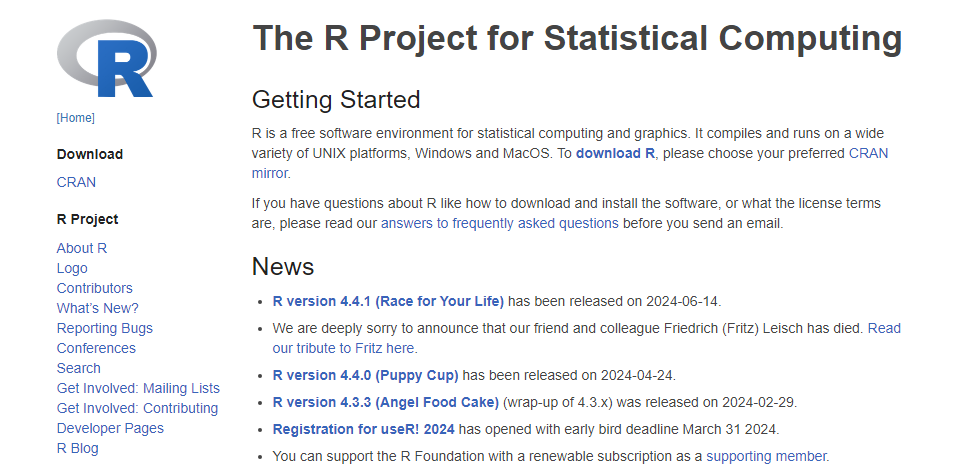
\includegraphics{images/r-proj-site.png} \emph{Screenshot of the R Project homepage, where R can be downloaded.}

\hypertarget{features-of-r}{%
\subsection{Features of R}\label{features-of-r}}

\begin{itemize}
\tightlist
\item
  \textbf{Statistical Analysis}: Provides a wide array of techniques for data analysis, including linear and nonlinear modeling, classical statistical tests, time-series analysis, classification, clustering, and more.
\item
  \textbf{Graphics}: Boasts high-quality graphics capabilities that allow for the creation of well-designed publications and interactive visualizations for the web.
\item
  \textbf{Packages}: Comes with a comprehensive ecosystem of packages, available through the Comprehensive R Archive Network (CRAN), which extend R's capabilities to handle tasks related to psychological research and beyond.
\item
  \textbf{Programming}: Supports both procedural programming with functions and object-oriented programming with generic functions.
\item
  \textbf{Community Support}: Has a large, active community offering support through mailing lists, forums, and blogs.
\end{itemize}

\hypertarget{what-is-r-studio}{%
\section{What is R Studio?}\label{what-is-r-studio}}

R Studio is an integrated development environment (IDE) for R.
It provides a user-friendly interface that makes using R easier and more efficient.
R Studio includes a console, syntax-highlighting editor that supports direct code execution, and tools for plotting, history, debugging, and workspace management.

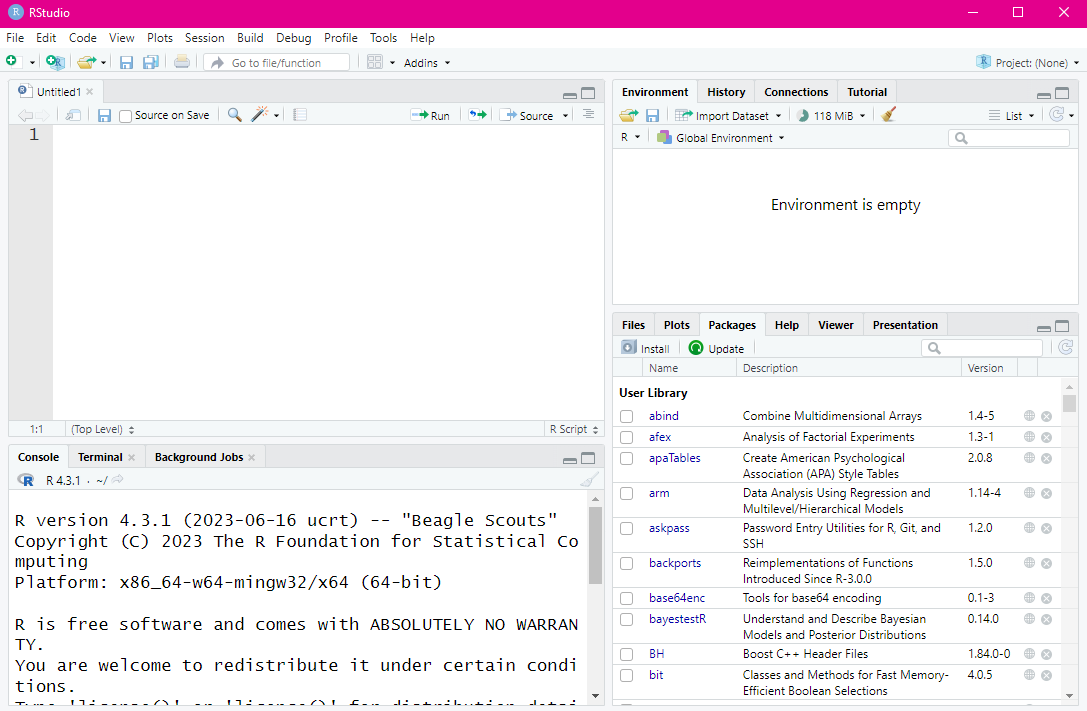
\includegraphics{images/r-studio.png} \emph{Overview of the R Studio interface.}

\hypertarget{why-use-r-studio}{%
\subsection{Why Use R Studio?}\label{why-use-r-studio}}

\begin{itemize}
\tightlist
\item
  \textbf{Ease of Use}: The R Studio environment organizes everything you need to write code, visualize data, and debug errors in one place.
\item
  \textbf{Productivity Tools}: Features like code completion, snippets, and the ability to directly output graphs enhance productivity.
\item
  \textbf{Project Management}: Simplifies the process of managing files associated with specific projects, making it easy to handle multiple, complex research projects.
\item
  \textbf{Reproducibility}: Encourages reproducible research by integrating well with R Markdown, which allows you to create dynamic reports that blend R code with narrative text and output.
\end{itemize}

\hypertarget{r-and-r-studio-in-psychological-research}{%
\section{R and R Studio in Psychological Research}\label{r-and-r-studio-in-psychological-research}}

In psychological research, R and R Studio play a critical role in: - \textbf{Data Collection and Cleaning}: Handling and cleaning raw data from experiments or surveys.
- \textbf{Statistical Testing}: Performing t-tests, ANOVA, regression analyses, and more sophisticated statistical models.
- \textbf{Data Visualization}: Creating compelling visualizations to explore data trends and communicate results.
- \textbf{Reproducible Research}: Producing reproducible analyses that can be shared and verified by others, enhancing the transparency and credibility of research findings.

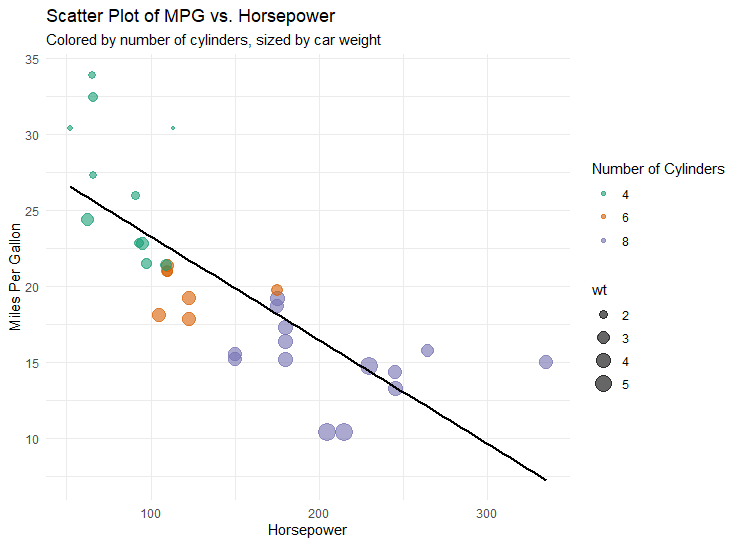
\includegraphics{images/ch1-Rplot.png} \emph{Example of a data visualization created in R.}

In the next sections, we will guide you through installing R and R Studio on your system and begin exploring their capabilities through practical exercises.
This foundation will set you up for success as you dive deeper into the statistical techniques and tools that will be covered throughout this course.

\hypertarget{installing-r}{%
\section{Installing R}\label{installing-r}}

To utilize R and R Studio for your statistical analysis, the first step is to install R.
R is the underlying statistical computing environment, while R Studio provides an integrated development environment (IDE) for R.
Below are the detailed instructions for installing R on Windows and macOS.

\hypertarget{installing-r-on-windows}{%
\subsection{Installing R on Windows}\label{installing-r-on-windows}}

Follow these steps to install R on a Windows computer:

\begin{enumerate}
\def\labelenumi{\arabic{enumi}.}
\item
  \textbf{Visit the CRAN Website}: Go to the Comprehensive R Archive Network (CRAN) at \url{https://cran.r-project.org}.
  This website hosts the R software and its documentation.
\item
  \textbf{Download R for Windows}: Click on the link titled ``Download R for Windows''.
  This will take you to the Windows download page.

  \begin{figure}
  \centering
  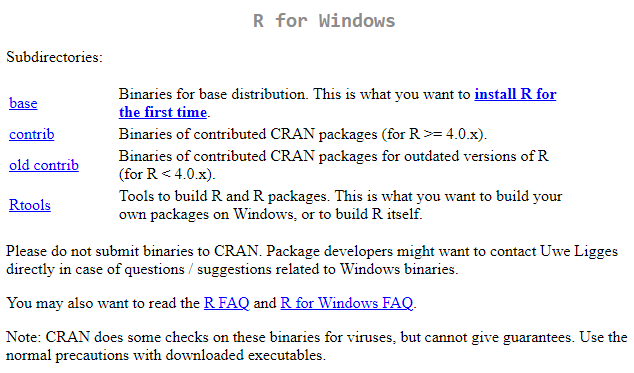
\includegraphics{images/r-windows.png}
  \caption{CRAN Homepage}
  \end{figure}
\item
  \textbf{Install R Base}: On the download page, click ``install R for the first time'' to navigate to the base distribution page.
  There, download the latest version of R by clicking the link at the top of the page.

  \begin{figure}
  \centering
  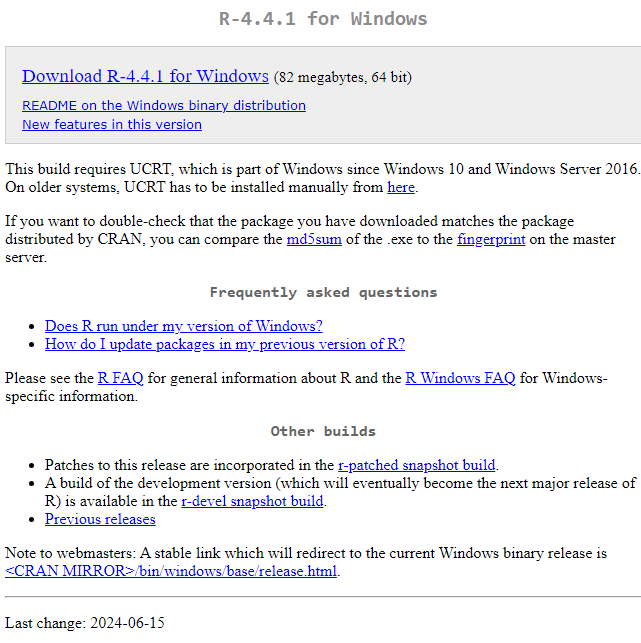
\includegraphics{images/r-windows-1st.png}
  \caption{Download R for Windows}
  \end{figure}
\item
  \textbf{Run the Installer}: Once the download is complete, open the executable file to start the installation process.
  Follow the prompts in the installer, accepting the default settings for a standard installation.
\item
  \textbf{Complete the Installation}: After following the installation prompts, click `Finish' to complete the installation.
\end{enumerate}

\hypertarget{installing-r-on-macos}{%
\subsection{Installing R on macOS}\label{installing-r-on-macos}}

Follow these steps to install R on a macOS computer:

\begin{enumerate}
\def\labelenumi{\arabic{enumi}.}
\item
  \textbf{Visit the CRAN Website}: Navigate to \url{https://cran.r-project.org} to access the CRAN homepage.
\item
  \textbf{Download R for macOS}: Click on the ``Download R for (Mac) OS X'' link to go to the macOS download page.

  \begin{figure}
  \centering
  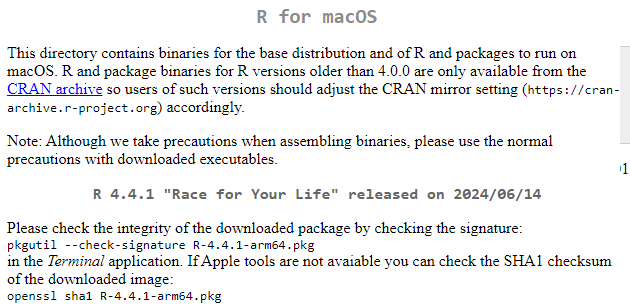
\includegraphics{images/r-mac.png}
  \caption{CRAN Homepage}
  \end{figure}
\item
  \textbf{Install R Package}: On the macOS download page, select the package suitable for your version of macOS.
  Click on the link to download the \texttt{.pkg} installer file.

  \begin{figure}
  \centering
  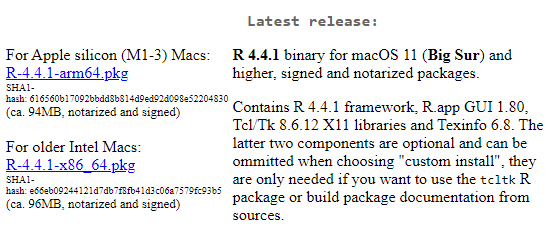
\includegraphics{images/r-mac-version.png}
  \caption{Download R for macOS}
  \end{figure}
\item
  \textbf{Run the Installer}: After the download is complete, double-click on the \texttt{.pkg} file to open the installer.
  Follow the on-screen instructions, accepting the default options where suggested.
\item
  \textbf{Complete the Installation}: Proceed through the installer by clicking `Continue' and then `Install'.
  You may need to enter your administrator password.
  Click `Finish' once the installation process completes.
\end{enumerate}

\hypertarget{verify-installation}{%
\subsection{Verify Installation}\label{verify-installation}}

After installing R on your system, it's a good idea to verify that it was installed correctly:

\begin{itemize}
\tightlist
\item
  \textbf{Open R}: Search for R in your applications (Windows) or use Spotlight (macOS) to find and launch R.
\item
  \textbf{Check Version}: In the R console, type \texttt{version} and press Enter. This will display information about the R version installed on your computer.
\end{itemize}

\begin{Shaded}
\begin{Highlighting}[]
\NormalTok{version}
\end{Highlighting}
\end{Shaded}

\hypertarget{installing-r-studio}{%
\section{Installing R Studio}\label{installing-r-studio}}

Once R is installed on your computer, the next step is to install R Studio, which will serve as your primary interface for writing and running R scripts.
Here are step-by-step instructions to install R Studio on both Windows and macOS.

\hypertarget{before-you-install}{%
\subsection{Before You Install}\label{before-you-install}}

Before installing R Studio, make sure that: - \textbf{R is Installed}: R Studio requires R to be installed on your computer.
If you haven't installed R yet, please refer to the previous section for instructions.
- \textbf{System Requirements}: Check the R Studio website for the latest system requirements to ensure compatibility with your operating system.

\hypertarget{installing-r-studio-on-windows}{%
\subsection{Installing R Studio on Windows}\label{installing-r-studio-on-windows}}

Follow these steps to install R Studio on a Windows computer:

\begin{enumerate}
\def\labelenumi{\arabic{enumi}.}
\item
  \textbf{Download R Studio}: Visit the Posit website at \url{https://posit.co/download/rstudio-desktop/} and navigate to the Download R Studio Desktop section.
  Click on the ``Download RStudio Desktop for Windows'' button.

  \begin{figure}
  \centering
  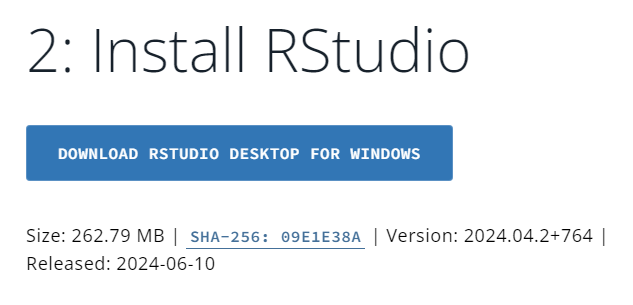
\includegraphics{images/r-studio-windows.png}
  \caption{Download R Studio for Windows}
  \end{figure}
\item
  \textbf{Run the Installer}: After the download is complete, open the executable file to start the installation process.
  You may receive a security warning; click `Run' to proceed.
\item
  \textbf{Follow the Installation Prompts}: The installer will guide you through the setup process.
  Accept the license agreement and keep the default installation settings unless you have specific preferences.
\item
  \textbf{Complete the Installation}: Click `Finish' to complete the installation process.
  R Studio should now be installed on your computer.
\end{enumerate}

\hypertarget{installing-r-studio-on-macos}{%
\subsection{Installing R Studio on macOS}\label{installing-r-studio-on-macos}}

Follow these steps to install R Studio on a macOS computer:

\begin{enumerate}
\def\labelenumi{\arabic{enumi}.}
\item
  \textbf{Download R Studio}: Visit the Posit website at \url{https://posit.co/download/rstudio-desktop/} and navigate to the Downloads table.
  Select the macOS linked file to download R Studio Desktop

  \begin{figure}
  \centering
  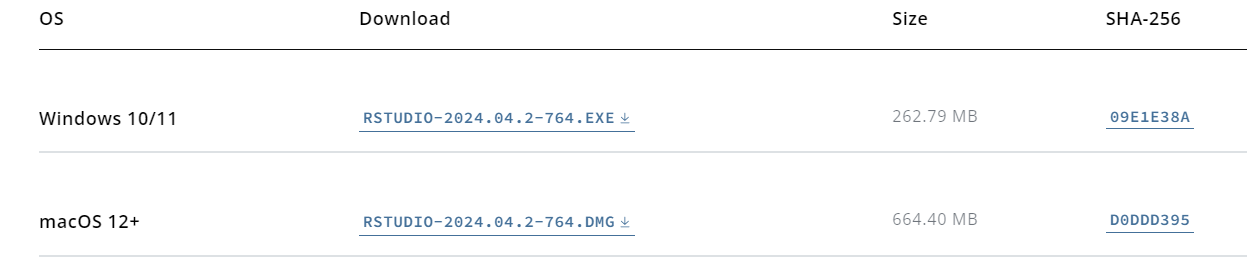
\includegraphics{images/r-studio-mac.png}
  \caption{Download R Studio for macOS}
  \end{figure}
\item
  \textbf{Open the Installer}: After the download, locate the \texttt{.dmg} file in your Downloads folder and double-click to open it.
\item
  \textbf{Drag R Studio to Applications}: A new window will open showing the R Studio icon.
  Drag this icon to your Applications folder to install the application.
\item
  \textbf{Complete the Installation}: Double-click R Studio from your Applications folder to ensure it opens correctly and completes any setup it requires the first time it runs.
\end{enumerate}

\hypertarget{verify-installation-1}{%
\subsection{Verify Installation}\label{verify-installation-1}}

To verify that R Studio is correctly installed: - \textbf{Launch R Studio}: Open R Studio from your Applications menu (Windows) or your Applications folder (macOS).
- \textbf{Check for R Version}: In the R Studio console, you should see the version of R that is being used by R Studio.

\begin{Shaded}
\begin{Highlighting}[]
\FunctionTok{sessionInfo}\NormalTok{()  }\CommentTok{\# This will print out your R session information, including R version.}
\end{Highlighting}
\end{Shaded}

\hypertarget{understanding-the-r-studio-interface}{%
\section{Understanding the R Studio Interface}\label{understanding-the-r-studio-interface}}

R Studio is a powerful integrated development environment (IDE) designed to make working with R more efficient and user-friendly.
Understanding the layout and functionalities of the R Studio interface is crucial for effective data analysis.
This section will guide you through the various components of the R Studio interface.

\hypertarget{the-r-studio-layout}{%
\subsection{The R Studio Layout}\label{the-r-studio-layout}}

R Studio's interface is divided into four main panes, each serving distinct functions that are essential for various aspects of programming and data analysis.
Here's an overview of these panes and their default configurations:

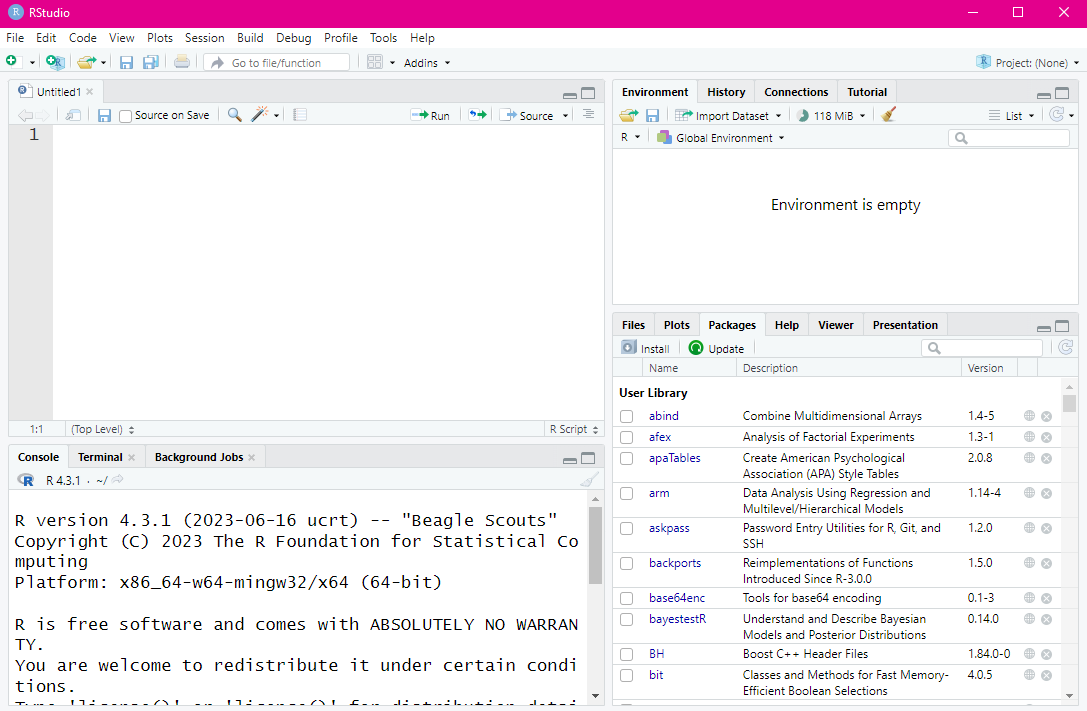
\includegraphics{images/r-studio.png} \emph{Overview of the R Studio interface.}

\hypertarget{purpose-of-each-pane}{%
\subsection{Purpose of Each Pane}\label{purpose-of-each-pane}}

\begin{enumerate}
\def\labelenumi{\arabic{enumi}.}
\tightlist
\item
  \textbf{Console Pane}

  \begin{itemize}
  \tightlist
  \item
    \textbf{Description}: This is where R scripts are executed. You can type R commands directly into the console and see the output of these commands.
  \item
    \textbf{Importance}: It's crucial for trying out quick commands and viewing their output immediately. 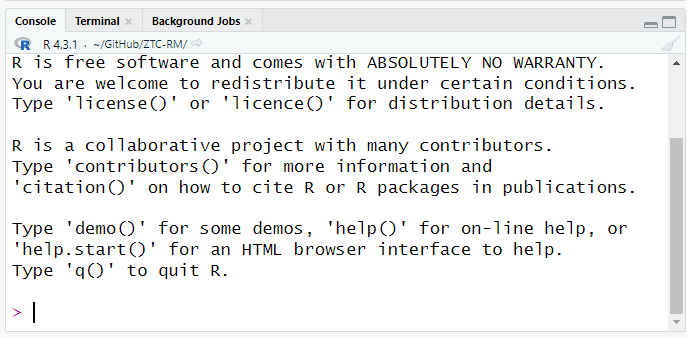
\includegraphics{images/r-console.png}
  \end{itemize}
\item
  \textbf{Source Pane}

  \begin{itemize}
  \tightlist
  \item
    \textbf{Description}: This pane is used for writing and editing scripts. Scripts are essentially files containing a series of R commands.
  \item
    \textbf{Importance}: The source pane allows for more complex script development, which can be saved, shared, and run repeatedly. 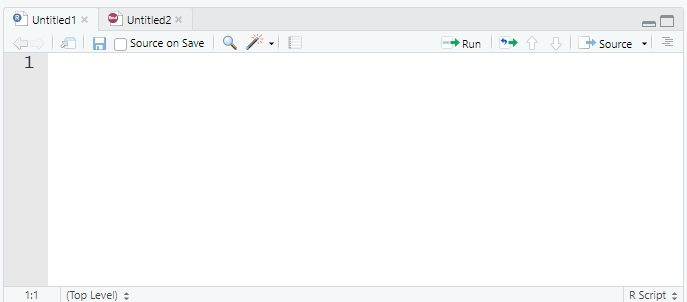
\includegraphics{images/r-source.png}
  \end{itemize}
\item
  \textbf{Environment/History Pane}

  \begin{itemize}
  \tightlist
  \item
    \textbf{Description}: The Environment tab shows the current working dataset and variables stored in memory. The History tab tracks the commands that have been executed.
  \item
    \textbf{Importance}: This pane is vital for managing the objects in your current R session and reviewing or re-running previous commands. 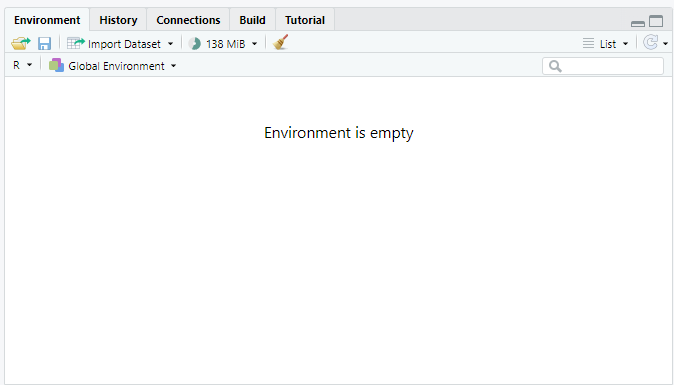
\includegraphics{images/r-env.png}
  \end{itemize}
\item
  \textbf{Files/Plots/Packages/Help/Viewer Pane}

  \begin{itemize}
  \tightlist
  \item
    \textbf{Description}: This multifunctional pane allows users to navigate files, view plots, manage R packages, access R documentation (Help), and view web content (Viewer).
  \item
    \textbf{Importance}: It supports a wide range of activities from managing the files related to your projects, visualizing data outputs, installing and loading libraries, seeking help on functions, and displaying HTML content. 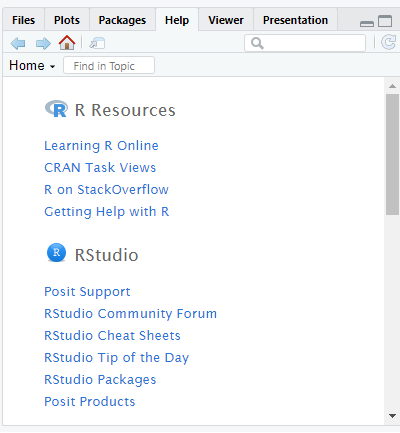
\includegraphics{images/r-help.png}
  \end{itemize}
\end{enumerate}

\hypertarget{navigating-and-customizing-the-interface}{%
\subsection{Navigating and Customizing the Interface}\label{navigating-and-customizing-the-interface}}

R Studio's layout is highly customizable.
You can adjust the size and location of the panes according to your preferences:

\begin{itemize}
\tightlist
\item
  \textbf{Resizing Panes}: You can resize any pane by dragging the borders between them.
\item
  \textbf{Repositioning Panes}: Under the \texttt{Tools} menu, select \texttt{Global\ Options}, then \texttt{Pane\ Layout} to customize the arrangement of the workspace.
\item
  \textbf{Customizing Appearance}: Change the theme of your R Studio interface by navigating to \texttt{Tools} \textgreater{} \texttt{Global\ Options} \textgreater{} \texttt{Appearance}. You can select different editor themes and adjust font size to suit your visual preferences.
\end{itemize}

\hypertarget{best-practices}{%
\subsection{Best Practices}\label{best-practices}}

\begin{itemize}
\tightlist
\item
  \textbf{Familiarize Early}: Spend some time exploring and customizing the R Studio interface to suit your workflow. This familiarity will increase your productivity.
\item
  \textbf{Keyboard Shortcuts}: Learn and utilize R Studio keyboard shortcuts to speed up your coding and navigation. You can find a list of shortcuts by pressing \texttt{Alt\ +\ Shift\ +\ K}.
\end{itemize}

\begin{center}\rule{0.5\linewidth}{0.5pt}\end{center}

Understanding the layout and functionality of the R Studio interface is the first step toward mastering R for statistical analysis.
As you become more familiar with these tools, you'll find that R Studio enhances your efficiency and effectiveness in data analysis tasks.

\hypertarget{basics-of-using-r-studio}{%
\section{Basics of Using R Studio}\label{basics-of-using-r-studio}}

R Studio enhances the usability of R by providing an organized work environment with powerful tools for data analysis and script management.
This section will guide you through creating and managing R scripts and documents, and provide a thorough introduction to using R Markdown for your assignments.

\hypertarget{creating-and-saving-r-scripts}{%
\subsection{Creating and Saving R Scripts}\label{creating-and-saving-r-scripts}}

\hypertarget{creating-a-new-script}{%
\subsubsection{Creating a New Script}\label{creating-a-new-script}}

To begin scripting in R:

\begin{enumerate}
\def\labelenumi{\arabic{enumi}.}
\tightlist
\item
  \textbf{Open R Studio} and click on \texttt{File} in the menu bar.
\item
  Select \texttt{New\ File} and then \texttt{R\ Script}. This will open a new script tab in the Source Pane.
\end{enumerate}

\begin{figure}
\centering
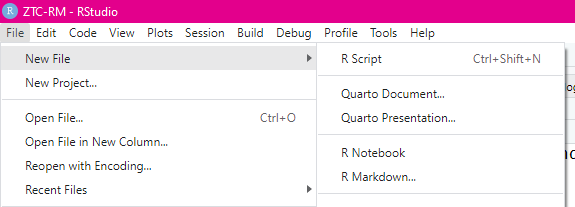
\includegraphics{images/r-new_script.png}
\caption{Create New R Script}
\end{figure}

\hypertarget{saving-scripts}{%
\subsubsection{Saving Scripts}\label{saving-scripts}}

To save your script:

\begin{enumerate}
\def\labelenumi{\arabic{enumi}.}
\tightlist
\item
  Click on the floppy disk icon or press \texttt{Ctrl\ +\ S} (Windows) or \texttt{Cmd\ +\ S} (macOS).
\item
  Choose a location on your computer, name your file, and ensure it has the \texttt{.R} extension.
\end{enumerate}

\begin{figure}
\centering
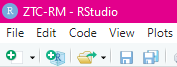
\includegraphics{images/r-floppy.png}
\caption{Save R Script}
\end{figure}

\hypertarget{writing-and-executing-code}{%
\subsection{Writing and Executing Code}\label{writing-and-executing-code}}

\hypertarget{writing-code}{%
\subsubsection{Writing Code}\label{writing-code}}

\begin{itemize}
\tightlist
\item
  Write your R code in the Source Pane. This should be used for scripts that you might want to save, reuse, or share.
\item
  Avoid writing scripts directly in the Console as it is meant for temporary tests and does not save your commands.
\end{itemize}

\hypertarget{executing-code}{%
\subsubsection{Executing Code}\label{executing-code}}

\begin{itemize}
\tightlist
\item
  To run code from the Source Pane, select the line(s) of code you want to execute and press \texttt{Ctrl\ +\ Enter} (Windows) or \texttt{Cmd\ +\ Enter} (macOS).
\item
  The results will appear in the Console Pane.
\end{itemize}

\hypertarget{importing-data}{%
\subsection{Importing Data}\label{importing-data}}

To import data into R Studio:

\begin{enumerate}
\def\labelenumi{\arabic{enumi}.}
\tightlist
\item
  Use the \texttt{read.csv()} function for CSV files: \texttt{data\ \textless{}-\ read.csv("path/to/your/datafile.csv")}
\item
  You can also use the Import Dataset feature in the Environment Pane for a GUI approach.
\end{enumerate}

\begin{figure}
\centering
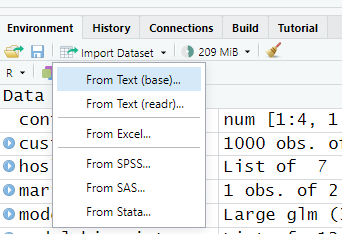
\includegraphics{images/r-import.png}
\caption{Import Data}
\end{figure}

\hypertarget{using-r-markdown-for-assignments}{%
\subsection{Using R Markdown for Assignments}\label{using-r-markdown-for-assignments}}

R Markdown allows you to integrate text, code, and their outputs into a single document.

\hypertarget{what-is-r-markdown}{%
\subsubsection{What is R Markdown?}\label{what-is-r-markdown}}

R Markdown files, ending in \texttt{.Rmd}, let you create dynamic documents, presentations, and reports from R.
It integrates your R code with Markdown text and can output to formats like PDF, HTML, and Word.

\hypertarget{basic-markdown-syntax}{%
\subsubsection{Basic Markdown Syntax}\label{basic-markdown-syntax}}

\begin{itemize}
\tightlist
\item
  \textbf{Headers}: \texttt{\#} for main headers, \texttt{\#\#} for subheaders
\item
  \textbf{Bold}: \texttt{**bold\ text**}
\item
  \textbf{Italics}: \texttt{*italicized\ text*}
\item
  \textbf{Lists}: Use \texttt{-} or \texttt{*} for unordered lists and \texttt{1.}, \texttt{2.}, etc., for ordered lists.
\item
  \textbf{Links}: \texttt{{[}Link\ text{]}(URL)}
\item
  \textbf{Images}: \texttt{!{[}Alt\ text{]}(path/to/image)}
\item
  \textbf{Code}: Use backticks \texttt{\textasciigrave{}} for inline code and triple backticks \texttt{\textasciigrave{}\textasciigrave{}\textasciigrave{}} for code blocks.
\end{itemize}

\hypertarget{creating-an-r-markdown-file}{%
\subsubsection{Creating an R Markdown File}\label{creating-an-r-markdown-file}}

\begin{enumerate}
\def\labelenumi{\arabic{enumi}.}
\tightlist
\item
  Go to \texttt{File\ \textgreater{}\ New\ File\ \textgreater{}\ R\ Markdown...}.
\item
  Fill out the dialog box (title, author, and output format).
\end{enumerate}

\begin{figure}
\centering
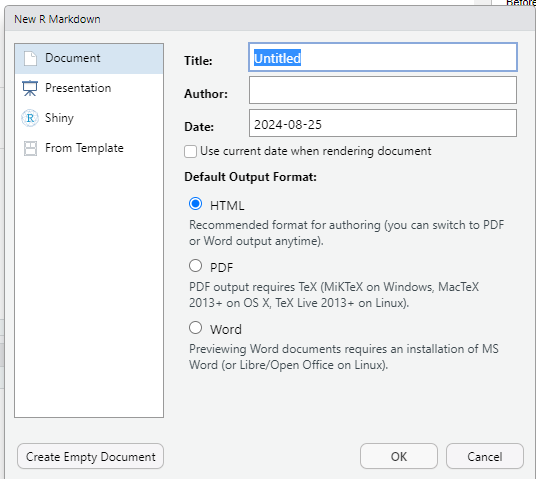
\includegraphics{images/r-rmd.png}
\caption{New R Markdown File}
\end{figure}

\hypertarget{writing-in-r-markdown}{%
\subsubsection{Writing in R Markdown}\label{writing-in-r-markdown}}

\begin{itemize}
\tightlist
\item
  Write narrative text using Markdown.
\item
  Insert code chunks using triple backticks and \texttt{r} to start each chunk:
\end{itemize}

```\texttt{\{r\}}

\begin{itemize}
\tightlist
\item
  Insert triple backticks to close a code chunk.\\
\item
  A code chunk will look like this:\\
  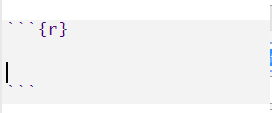
\includegraphics{images/r-chunk.png}
\end{itemize}

\hypertarget{using-r-markdown-for-assignments-1}{%
\section{Using R Markdown for Assignments}\label{using-r-markdown-for-assignments-1}}

R Markdown allows you to integrate text, code, and their outputs into a single document, making it an invaluable tool for creating dynamic reports and presentations.
Here, we'll explore how to use R Markdown effectively in your assignments.

\hypertarget{what-is-r-markdown-1}{%
\subsection{What is R Markdown?}\label{what-is-r-markdown-1}}

R Markdown files, ending in \texttt{.Rmd}, allow you to integrate narrative text with embedded R code chunks in a single document.
It supports dynamic output generation in multiple formats, including HTML, PDF, and Word, making it ideal for academic and professional presentations.

\hypertarget{benefits-of-using-r-markdown}{%
\subsection{Benefits of Using R Markdown}\label{benefits-of-using-r-markdown}}

\begin{itemize}
\tightlist
\item
  \textbf{Reproducibility}: Automatically reproduce your findings by rerunning the R code embedded in your document.
\item
  \textbf{Dynamic Reporting}: Update data results and text simultaneously, ensuring consistency and accuracy in reports.
\item
  \textbf{Versatility}: Generate reports in various formats from a single source file, tailored for different audiences.
\end{itemize}

\hypertarget{basic-structure-of-an-r-markdown-document}{%
\subsection{Basic Structure of an R Markdown Document}\label{basic-structure-of-an-r-markdown-document}}

An R Markdown document is composed of three main parts:

\begin{itemize}
\tightlist
\item
  \textbf{YAML Header}: Specifies document settings such as title, output formats, and options.
\item
  \textbf{Narrative Text}: Written using Markdown for formatting.
\item
  \textbf{Code Chunks}: Embedded R code that can be executed to produce results directly in the document.
\end{itemize}

\hypertarget{yaml-header}{%
\subsubsection{YAML Header}\label{yaml-header}}

Here's an example YAML header that specifies the document title, author, and desired output formats:

\begin{Shaded}
\begin{Highlighting}[]
\PreprocessorTok{{-}{-}{-}}
\FunctionTok{title}\KeywordTok{:}\AttributeTok{ }\StringTok{"Your Analysis Report"}
\FunctionTok{author}\KeywordTok{:}\AttributeTok{ }\StringTok{"Your Name"}
\FunctionTok{date}\KeywordTok{:}\AttributeTok{ }\StringTok{"2024{-}08{-}25"}
\FunctionTok{output}\KeywordTok{:}
\AttributeTok{  }\FunctionTok{html\_document}\KeywordTok{:}
\AttributeTok{    }\FunctionTok{toc}\KeywordTok{:}\AttributeTok{ }\CharTok{true}
\AttributeTok{    }\FunctionTok{toc\_float}\KeywordTok{:}\AttributeTok{ }\CharTok{true}
\AttributeTok{  }\FunctionTok{pdf\_document}\KeywordTok{:}
\AttributeTok{    }\FunctionTok{toc}\KeywordTok{:}\AttributeTok{ }\CharTok{true}
\PreprocessorTok{{-}{-}{-}}
\end{Highlighting}
\end{Shaded}

\hypertarget{creating-an-r-markdown-file-1}{%
\subsubsection{Creating an R Markdown File}\label{creating-an-r-markdown-file-1}}

To create an R Markdown file in R Studio:

\begin{enumerate}
\def\labelenumi{\arabic{enumi}.}
\tightlist
\item
  Click \texttt{File} \textgreater{} \texttt{New\ File} \textgreater{} \texttt{R\ Markdown...}.
\item
  Provide the title and author name, and select the default output format.
\end{enumerate}

\hypertarget{writing-markdown}{%
\subsubsection{Writing Markdown}\label{writing-markdown}}

Markdown is a simple formatting syntax for authoring HTML, PDF, and MS Word documents.
Here are some basics:

\begin{itemize}
\tightlist
\item
  \textbf{Headings}: \texttt{\#} for level 1 header, \texttt{\#\#} for level 2, and so on.
\item
  \textbf{Bold}: \texttt{**bold\ text**}
\item
  \textbf{Italics}: \texttt{*italicized\ text*}
\item
  \textbf{Lists}: \texttt{-} or \texttt{*} for bullet points, \texttt{1.}, \texttt{2.}, etc., for numbered lists.
\item
  \textbf{Links}: \texttt{{[}text{]}(URL)}
\item
  \textbf{Images}: \texttt{!{[}description{]}(path)}
\end{itemize}

\hypertarget{including-code-chunks}{%
\subsubsection{Including Code Chunks}\label{including-code-chunks}}

Insert R code within your narrative by enclosing it in triple backticks:

\begin{Shaded}
\begin{Highlighting}[]
\FunctionTok{summary}\NormalTok{(cars)}
\end{Highlighting}
\end{Shaded}

\begin{verbatim}
##      speed           dist       
##  Min.   : 4.0   Min.   :  2.00  
##  1st Qu.:12.0   1st Qu.: 26.00  
##  Median :15.0   Median : 36.00  
##  Mean   :15.4   Mean   : 42.98  
##  3rd Qu.:19.0   3rd Qu.: 56.00  
##  Max.   :25.0   Max.   :120.00
\end{verbatim}

\hypertarget{knitting-documents}{%
\subsection{Knitting Documents}\label{knitting-documents}}

Knitting refers to the process of converting an R Markdown file into a specified output format.
To knit your document:

\begin{itemize}
\tightlist
\item
  Click the \texttt{Knit} button in R Studio and choose the output format (HTML, PDF, or Word).
\item
  R Studio will execute the embedded R code chunks and generate the final document.
\end{itemize}

\hypertarget{output-file-location}{%
\subsubsection{Output File Location}\label{output-file-location}}

Knitted files are saved in the same directory as the \texttt{.Rmd} file by default.
Use the Files pane in R Studio to navigate and find these documents.

\hypertarget{best-practices-1}{%
\subsection{Best Practices}\label{best-practices-1}}

\begin{itemize}
\tightlist
\item
  \textbf{Regularly Save Your Work}: Ensure you save your \texttt{.Rmd} file frequently.
\item
  \textbf{Version Control}: Use version control systems like Git to manage changes and collaborate effectively.
\item
  \textbf{Document Your Code}: Comment your R code within chunks to explain what each part does.
\end{itemize}

\begin{center}\rule{0.5\linewidth}{0.5pt}\end{center}

R Markdown is a robust tool for statistical analysis and report generation.
Mastering its use will enhance the clarity and impact of your research presentations and assignments.

\hypertarget{best-practices-2}{%
\section{Best Practices}\label{best-practices-2}}

Effective use of R Studio and R Markdown involves more than just knowing the tools; it also requires adopting practices that enhance productivity, ensure reproducibility, and maintain the quality of your work.
This section outlines some best practices that you should follow when working with R and R Markdown.

\hypertarget{keep-scripts-organized}{%
\subsection{Keep Scripts Organized}\label{keep-scripts-organized}}

Organization is key to managing complex projects, especially when dealing with numerous datasets and scripts.

\begin{itemize}
\tightlist
\item
  \textbf{Project Folders}: Create separate folders for each project to keep files related to that project together.
\item
  \textbf{Descriptive Filenames}: Use clear and descriptive filenames that reflect the content or purpose of each script or dataset.
\end{itemize}

\hypertarget{comment-your-code}{%
\subsection{Comment Your Code}\label{comment-your-code}}

Comments are crucial for explaining what your code does, both to others and to your future self.

\begin{itemize}
\tightlist
\item
  \textbf{Clarity}: Write comments that clearly explain the purpose of each section of your code.
\item
  \textbf{Consistency}: Develop a consistent style for your comments, such as starting each comment with a capital letter and ending with a period.
\item
  \textbf{Coverage}: Comment liberally throughout your code to explain why you made certain coding choices.
\end{itemize}

\begin{Shaded}
\begin{Highlighting}[]
\FunctionTok{\# Calculate mean speed {-} this is used for initial speed analysis}
\NormalTok{mean\_speed \textless{}{-} mean(data$speed)}
\end{Highlighting}
\end{Shaded}

\hypertarget{use-version-control}{%
\subsection{Use Version Control}\label{use-version-control}}

Version control systems like Git are invaluable for managing changes to your documents and code, especially in collaborative projects.

\begin{itemize}
\item
  \textbf{Track Changes}: Use Git to track changes in your scripts, allowing you to revert to previous versions if necessary.
\item
  \textbf{Collaboration}: Version control makes collaborating on projects easier, as it allows multiple people to work on the same files without conflict.
\item
  \textbf{Backup}: Regularly push your changes to a remote repository like GitHub for backup and sharing purposes.
\end{itemize}

\hypertarget{regularly-save-and-backup-your-work}{%
\subsection{Regularly Save and Backup Your Work}\label{regularly-save-and-backup-your-work}}

Losing data or scripts can be a significant setback, so regular backups are essential.

\begin{itemize}
\item
  \textbf{Local Backups}: Regularly save your work on your local machine.
  Consider setting up automated backups if available.
\item
  \textbf{Remote Backups}: Use cloud storage services or remote servers to keep a backup of your work.
  This protects against local hardware failures.
\end{itemize}

\hypertarget{write-readable-and-maintainable-code}{%
\subsection{Write Readable and Maintainable Code}\label{write-readable-and-maintainable-code}}

Readable code is more maintainable, easier to share with others, and easier to debug.

\begin{itemize}
\item
  \textbf{Formatting}: Use consistent indentation and spacing in your scripts.
\item
  \textbf{Simplify}: Break complex operations into simpler steps that are easier to understand and test.
\end{itemize}

\hypertarget{document-your-processes}{%
\subsection{Document Your Processes}\label{document-your-processes}}

Documentation is not just about commenting on your code; it also involves keeping records of your research processes and decisions.

\begin{itemize}
\item
  \textbf{Codebooks}: Create codebooks for your datasets, describing each variable and how it is coded.
\item
  \textbf{Research Diary}: Keep a diary of your research decisions, especially why certain analyses were chosen and what the outcomes were.
\end{itemize}

\hypertarget{knit-documents-regularly}{%
\subsection{Knit Documents Regularly}\label{knit-documents-regularly}}

For R Markdown documents, regular knitting can help you catch errors and see the effects of your code changes in the output document.

\begin{itemize}
\tightlist
\item
  \textbf{Iterative Knitting}: Knit your document after significant changes to ensure that your document compiles correctly and your changes produce the expected results.
\end{itemize}

\hypertarget{optimize-workflow-in-r-studio}{%
\subsection{Optimize Workflow in R Studio}\label{optimize-workflow-in-r-studio}}

R Studio offers many tools to optimize your workflow:

\begin{itemize}
\item
  \textbf{R Studio Projects}: Use R Studio Projects to manage all files associated with a project in one place.
\item
  \textbf{Keyboard Shortcuts}: Learn and use keyboard shortcuts in R Studio to speed up your workflow. (Example - Insert a chunk: Ctrl + Alt + I (Windows) or Cmd + Option + I (Mac))
\end{itemize}

\begin{center}\rule{0.5\linewidth}{0.5pt}\end{center}

Adopting these best practices will help you use R Studio and R Markdown more effectively, enhancing the quality of your work and making your data analysis process more efficient and reproducible.

\hypertarget{chapter-summary}{%
\section{Chapter Summary}\label{chapter-summary}}

In this chapter, you have learned the fundamental skills necessary to begin working with R and R Studio. We explored the R Studio interface, detailing the purpose of each pane and how they contribute to an effective work environment. Additionally, we introduced R Markdown, a powerful tool for integrating code and documentation, which you'll use for creating dynamic reports and presentations.

We covered the basics of creating and saving R scripts, the importance of organizing your work, and best practices for writing clean, understandable code. Understanding these foundational concepts is crucial as they form the backbone of any data analysis project in R.

\hypertarget{exercises}{%
\section{Exercises}\label{exercises}}

To reinforce what you've learned in this chapter, try completing the following exercises:

\hypertarget{exercise-1-familiarization-with-r-studio}{%
\subsection{Exercise 1: Familiarization with R Studio}\label{exercise-1-familiarization-with-r-studio}}

\begin{enumerate}
\def\labelenumi{\arabic{enumi}.}
\tightlist
\item
  Create a new R script and save it with the name \texttt{practice\_script.R}.
\item
  In your new script, write a simple calculation, such as \texttt{8\ *\ 9}, and run this line of code using R Studio.
\item
  Use the comment functionality to note what the code does.
\end{enumerate}

\hypertarget{exercise-2-basic-data-entry-and-operation}{%
\subsection{Exercise 2: Basic Data Entry and Operation}\label{exercise-2-basic-data-entry-and-operation}}

\begin{enumerate}
\def\labelenumi{\arabic{enumi}.}
\tightlist
\item
  Create a vector of numbers from 1 to 10 and assign it to a variable named \texttt{numbers}.
\item
  Calculate the sum of the vector and print the result in the console.
\item
  Write the commands into an R script and save it.
\end{enumerate}

\hypertarget{exercise-3-introduction-to-r-markdown}{%
\subsection{Exercise 3: Introduction to R Markdown}\label{exercise-3-introduction-to-r-markdown}}

\begin{enumerate}
\def\labelenumi{\arabic{enumi}.}
\tightlist
\item
  Create a new R Markdown document titled ``My First R Markdown''.
\item
  Write a brief introduction about yourself using Markdown syntax (include at least one header, one list, and bold text).
\item
  Embed a chunk of R code that calculates the square of 12.
\item
  Knit the document to HTML and save the output.
\end{enumerate}

\hypertarget{exercise-4-exploring-the-help-pane}{%
\subsection{Exercise 4: Exploring the Help Pane}\label{exercise-4-exploring-the-help-pane}}

\begin{enumerate}
\def\labelenumi{\arabic{enumi}.}
\tightlist
\item
  Use the Help pane to find help on the \texttt{plot} function.
\item
  In a new R script, write a command to plot a simple graph using \texttt{plot(1:10,\ 1:10)}.
\item
  Add a title to the plot by referring to the help documentation.
\end{enumerate}

\hypertarget{conclusion}{%
\subsection{Conclusion}\label{conclusion}}

By completing these exercises, you will enhance your familiarity with R and R Studio's basic functions and capabilities. This practice will prepare you for more complex operations and analyses in upcoming chapters. Ensure to regularly save and organize your scripts as you progress through the course.

\hypertarget{types-of-data-psychologists-collect}{%
\chapter{Types of Data Psychologists Collect}\label{types-of-data-psychologists-collect}}

In psychological research, data serves as the foundation upon which scientific inquiries are built. The choice of data type directly influences the research design, the kind of questions that can be addressed, and the conclusions that can be drawn. Understanding different types of data and their implications is crucial for conducting robust and ethically sound research.

\hypertarget{why-data-collection-is-crucial}{%
\section{Why Data Collection is Crucial}\label{why-data-collection-is-crucial}}

Data collection in psychology allows researchers to quantify variables, test hypotheses, and draw conclusions about human behavior and mental processes. The integrity and appropriateness of the data collected determine the validity of the research findings. Without data, psychological research would rely merely on theory and speculation, lacking empirical evidence to support or refute these theories.

\hypertarget{impact-of-data-type-on-research-outcomes}{%
\section{Impact of Data Type on Research Outcomes}\label{impact-of-data-type-on-research-outcomes}}

The type of data collected in a study can dramatically impact the results and interpretations. Each data type, whether observational, self-report, or experimental manipulation, comes with its own set of strengths and weaknesses. These characteristics influence how researchers design studies and what limitations they may encounter in their experimental conclusions.

\label{tab:callout-box}Hypothetical Example on the Impact of Data Type

Hypothetical Example: The Role of Data in Psychology

Consider a hypothetical study designed to investigate the effects of different parenting styles on child behavior. In this scenario, researchers might choose to utilize \textbf{observational data} to authentically capture children's reactions to various parenting interventions in a controlled setting. This approach could allow for an objective analysis of behavioral outcomes, demonstrating how the selection of data type (observational rather than self-report) can critically influence the depth and validity of research findings.

This hypothetical example illustrates the pivotal role that data plays in psychological research. By opting for observational data, the researchers in this imagined study could minimize subjective biases often associated with self-report data, thus more effectively isolating and analyzing the variables under investigation.

\hypertarget{real-world-implications}{%
\section{Real-World Implications}\label{real-world-implications}}

The implications of data type selection extend beyond academic circles into real-world applications. For instance, in clinical psychology, the effectiveness of various therapeutic interventions is often assessed through both self-report data and observational data. Choosing the appropriate type of data can lead to more effective treatment plans and better patient outcomes.

Understanding the strengths and limitations of each data type is essential for designing effective studies that yield reliable and actionable insights. As we explore each data type in the following sections, consider how each might best be utilized in different research contexts.

\hypertarget{observational-data}{%
\section{Observational Data}\label{observational-data}}

Observational data is one of the most fundamental and frequently used types of data in psychological research. This section delves into what observational data entails, its advantages, and the challenges it presents.

\hypertarget{definition-and-examples}{%
\subsection{Definition and Examples}\label{definition-and-examples}}

Observational data in psychology is collected through direct observation of subjects' behavior in natural or controlled environments, without manipulation or intervention by the researcher. This method is designed to capture behavior in its natural state and can be qualitative or quantitative.

\label{tab:callout-example}Hypothetical Example of Observational Data

Example: Child Development Study

In a study on child development, researchers might observe how children interact with their peers in a playground setting. The observers would note behaviors related to social interaction, conflict resolution, and play patterns without interfering with the children's activities. This method provides genuine insights into the social behaviors and dynamics among children.

\hypertarget{advantages-of-observational-data}{%
\subsection{Advantages of Observational Data}\label{advantages-of-observational-data}}

Observational data offers several key advantages:

\begin{itemize}
\item
  \textbf{Authenticity}: Observations are made in real-time, often in natural settings, which can provide a more genuine and comprehensive understanding of the subject's behavior and interactions.
\item
  \textbf{Non-invasive}: By not interfering with the subjects, researchers can ensure that the behavior observed is not influenced by the presence of the study or the researcher, maintaining the natural dynamics of the situation.
\item
  \textbf{Rich Detail}: Observational data can capture nuances and subtleties in behavior that other data collection methods might miss.
\end{itemize}

\hypertarget{disadvantages-of-observational-data}{%
\subsection{Disadvantages of Observational Data}\label{disadvantages-of-observational-data}}

Despite its strengths, observational data also has several drawbacks:

\begin{itemize}
\item
  \textbf{Observer Bias}: The presence of the observer and their subjective interpretations can introduce bias. What the observer expects to see can influence what they notice and record.
\item
  \textbf{Lack of Control}: Observational studies often lack the control over variables that experimental designs offer. This can make it difficult to establish causal relationships between observed behaviors and environmental conditions.
\item
  \textbf{Time-Consuming}: Gathering observational data can be labor-intensive and time-consuming. It requires extensive time in the field, detailed note-taking, and often, lengthy periods of observation to gather enough data for analysis.
\end{itemize}

\hypertarget{ethical-considerations}{%
\subsection{Ethical Considerations}\label{ethical-considerations}}

When conducting observational research, especially in sensitive settings or with vulnerable populations, ethical considerations must be carefully managed. Researchers need to ensure that privacy is respected and that the observation does not alter the natural behavior of the participants.

\label{tab:callout-box2}Ethical Consideration in Observational Studies

Ethical Consideration: Observing without Intruding

In psychological research, it is crucial to maintain the confidentiality and anonymity of the participants. For instance, when observing children, researchers must obtain consent from guardians or parents and ensure that the children's identities are protected in any reports or publications.

\hypertarget{conclusion-1}{%
\subsection{Conclusion}\label{conclusion-1}}

Observational data provides valuable insights into natural behaviors and interactions. While it has its limitations, such as potential biases and the challenge of not being able to control variables, its strengths in capturing authentic and detailed behaviors make it indispensable in many psychological studies. Researchers must weigh these factors when choosing observational methods and consider ethical implications carefully to conduct responsible research.

\hypertarget{self-report-data}{%
\section{Self-Report Data}\label{self-report-data}}

Self-report data is a critical component of psychological research, providing insights directly from participants about their thoughts, feelings, behaviors, and experiences. This section explores what constitutes self-report data, its uses, advantages, and the inherent limitations.

\hypertarget{definition-and-examples-1}{%
\subsection{Definition and Examples}\label{definition-and-examples-1}}

Self-report data involves collecting information from study participants through their direct responses. This can include questionnaires, surveys, diaries, and interviews.

\label{tab:callout-example3}Hypothetical Example of Self-Report Data

Example: Mental Health Assessment

A common example of self-report data in psychology is the use of questionnaires to assess symptoms of depression or anxiety. Participants may be asked to rate their agreement with statements like `I have felt sad or hopeless almost every day in the past two weeks' on a Likert scale. This approach allows researchers to gather data on subjective experiences that are not easily observable.

\hypertarget{advantages-of-self-report-data}{%
\subsection{Advantages of Self-Report Data}\label{advantages-of-self-report-data}}

Self-report data is particularly valuable for several reasons:

\begin{itemize}
\item
  \textbf{Accessibility}: It is often easier and more cost-effective to collect than other types of data, especially for large samples.
\item
  \textbf{Insight into Subjectivity}: Self-report methods are unparalleled in providing direct insights into participants' personal perceptions, feelings, and experiences.
\item
  \textbf{Flexibility}: These tools can be used in a wide range of settings and populations, making them versatile for numerous psychological topics.
\end{itemize}

\hypertarget{disadvantages-of-self-report-data}{%
\subsection{Disadvantages of Self-Report Data}\label{disadvantages-of-self-report-data}}

Despite its advantages, self-report data also has significant drawbacks:

\begin{itemize}
\item
  \textbf{Response Biases}: Participants may consciously or unconsciously provide answers they believe are expected, socially acceptable, or cast them in a favorable light (social desirability bias).
\item
  \textbf{Recall Inaccuracies}: Participants may not accurately remember past events or experiences, leading to recall bias in their responses.
\item
  \textbf{Over-Simplification}: Simplified survey and questionnaire responses may not capture the complexity of what is being studied, particularly with nuanced psychological states or processes.
\end{itemize}

\hypertarget{methodological-considerations}{%
\subsection{Methodological Considerations}\label{methodological-considerations}}

To maximize the reliability and validity of self-report data, researchers must carefully design questions and choose the appropriate formats for data collection.

\label{tab:callout-example4}Improving the Accuracy of Self-Report Data

Methodological Tip: Question Design

To reduce the impact of social desirability bias, questions should be framed in a neutral manner that does not imply a `correct' or `desired' answer. Additionally, including reverse-scored items can help mitigate the tendency of participants to respond in socially desirable ways.

\hypertarget{conclusion-2}{%
\subsection{Conclusion}\label{conclusion-2}}

While self-report data is an indispensable tool in psychological research, it is crucial to be aware of its limitations. Proper question design, careful data handling, and combining self-report measures with other data types can enhance the robustness of the findings. Researchers must critically assess when and how to use self-report data to best understand the phenomena under study.

\hypertarget{experimental-manipulation}{%
\section{Experimental Manipulation}\label{experimental-manipulation}}

Experimental manipulation is a cornerstone of psychological research that involves altering variables to determine cause-and-effect relationships. This section explores how experimental manipulation is implemented in psychology, its unique ability to establish causality, and its limitations.

\hypertarget{definition-and-examples-2}{%
\subsection{Definition and Examples}\label{definition-and-examples-2}}

Experimental manipulation involves deliberately changing one variable (the independent variable) to observe the effect on another variable (the dependent variable), within a controlled environment. This method is pivotal in establishing causal relationships between variables.

\label{tab:callout-example5}Hypothetical Example of Experimental Manipulation

Example: Studying the Effect of Sleep on Cognitive Performance

Consider an experiment where the amount of sleep participants receive is manipulated across different nights, and their cognitive performance is measured the following day. This setup allows researchers to directly assess how variations in sleep (independent variable) affect cognitive abilities (dependent variable), while controlling for factors like nutrition and physical activity.

\hypertarget{causality-and-the-gold-standard-of-experimental-research}{%
\subsection{Causality and the Gold Standard of Experimental Research}\label{causality-and-the-gold-standard-of-experimental-research}}

Experimental manipulation is often referred to as the gold standard in research because it uniquely fulfills the three criteria necessary for establishing causality:

\begin{itemize}
\item
  \textbf{Association}: Experiments demonstrate an association between variables when changes in the independent variable systematically result in changes in the dependent variable.
\item
  \textbf{Temporal Precedence}: Experimental design ensures that the cause (manipulation of the independent variable) precedes the effect (changes in the dependent variable), establishing a chronological order.
\item
  \textbf{Controlling Extraneous Variables}: By controlling extraneous variables, experiments can isolate the effect of the independent variable on the dependent variable, minimizing confounding factors. This control is achieved through techniques like randomization, use of control groups, and standardized procedures, ensuring that any observed effects can be attributed directly to the manipulated variable.
\end{itemize}

\hypertarget{advantages-of-experimental-manipulation}{%
\subsection{Advantages of Experimental Manipulation}\label{advantages-of-experimental-manipulation}}

\begin{itemize}
\item
  \textbf{Strong Causal Inferences}: The rigorous control over variables allows researchers to draw strong causal inferences, a capability unmatched by non-experimental methods.
\item
  \textbf{Replicability}: The structured nature of experimental designs makes replication by other researchers feasible, which is essential for verifying and solidifying research findings.
\end{itemize}

\hypertarget{disadvantages-of-experimental-manipulation}{%
\subsection{Disadvantages of Experimental Manipulation}\label{disadvantages-of-experimental-manipulation}}

Despite its strengths, experimental manipulation also presents challenges:

\begin{itemize}
\item
  \textbf{Ethical Concerns}: Manipulating variables, especially in sensitive areas such as psychological stress or deprivation, can raise serious ethical concerns about the welfare of participants.
\item
  \textbf{Artificiality}: The controlled, often laboratory-based conditions necessary for experimental manipulation may not accurately reflect real-world scenarios, potentially limiting the generalizability of findings.
\item
  \textbf{Complexity and Cost}: Conducting experiments can be resource-intensive and complex, requiring detailed planning, specialized equipment, and sometimes significant financial investment.
\end{itemize}

\hypertarget{ethical-considerations-1}{%
\subsection{Ethical Considerations}\label{ethical-considerations-1}}

Ethical considerations are paramount when planning and conducting experiments, especially those involving potentially harmful interventions or vulnerable populations.

\label{tab:callout-box6}Ethical Considerations in Experimental Studies

Ethical Consideration: Ensuring Informed Consent

In experimental research, informed consent is crucial. Participants must be fully aware of the study's nature, any potential risks, and their right to withdraw at any time without any form of penalty.

\hypertarget{conclusion-3}{%
\subsection{Conclusion}\label{conclusion-3}}

Experimental manipulation remains a powerful method for exploring causal mechanisms in psychology. While it offers the unique ability to control variables and establish cause and effect, it also demands rigorous ethical scrutiny and thoughtful design to ensure relevance and applicability. Balancing these elements is crucial for conducting impactful and responsible psychological research.

\hypertarget{comparative-analysis}{%
\section{Comparative Analysis}\label{comparative-analysis}}

This section provides a comparative analysis of the three primary types of data discussed in this chapter---observational data, self-report data, and experimental manipulation. Understanding the comparative advantages and limitations of each data type helps researchers make informed decisions about their study designs and achieve more accurate and meaningful results.

\hypertarget{overview-of-data-types}{%
\subsection{Overview of Data Types}\label{overview-of-data-types}}

\begin{enumerate}
\def\labelenumi{\arabic{enumi}.}
\item
  \textbf{Observational Data}: Involves recording behaviors as they occur naturally or in structured environments without manipulation. Ideal for capturing genuine behaviors, but susceptible to observer biases and lacks control over variables.
\item
  \textbf{Self-Report Data}: Involves collecting information directly from participants about their feelings, thoughts, behaviors, and experiences. Provides direct subjective insights but can be affected by response biases and inaccuracies in self-assessment.
\item
  \textbf{Experimental Manipulation}: Involves manipulating one or more variables to determine their effect on other variables. Allows for strong causal inferences and control over extraneous variables, but may be artificial and ethically complex.
\end{enumerate}

\hypertarget{comparative-strengths}{%
\subsection{Comparative Strengths}\label{comparative-strengths}}

\begin{itemize}
\item
  \textbf{Authenticity and Detail}: Observational data excel in capturing detailed and authentic behaviors as they naturally unfold, providing a depth of qualitative information that is often unattainable through other methods.
\item
  \textbf{Subjective Insights and Accessibility}: Self-report data are unparalleled in accessing personal, subjective insights directly from participants, and are generally easy and cost-effective to collect, especially for large samples.
\item
  \textbf{Causal Relationships and Control}: Experimental manipulation is the only method that allows researchers to establish clear causal relationships due to the ability to control extraneous variables and directly manipulate the conditions of the study.
\end{itemize}

\hypertarget{comparative-weaknesses}{%
\subsection{Comparative Weaknesses}\label{comparative-weaknesses}}

\begin{itemize}
\item
  \textbf{Control and Bias}: Observational data often lack the control found in experimental designs, making them more susceptible to biases such as the observer's expectations influencing their recordings.
\item
  \textbf{Accuracy and Depth}: Self-report data can suffer from issues of accuracy due to memory recall errors and the desire to present oneself in a favorable light, potentially simplifying complex emotional or behavioral states.
\item
  \textbf{Artificiality and Ethical Concerns}: Experimental manipulation can create artificial situations that do not accurately reflect real-life scenarios, and ethical considerations must be carefully managed, especially when interventions could impact participants adversely.
\end{itemize}

\hypertarget{guidelines-for-choosing-data-types}{%
\subsection{Guidelines for Choosing Data Types}\label{guidelines-for-choosing-data-types}}

Choosing the right data type depends on the specific objectives and constraints of the research:

\begin{itemize}
\item
  \textbf{Research Question}: Consider what you need to measure to answer your research question. Use observational data to study behaviors in their natural context, self-report data to gauge internal states or perceptions, and experimental manipulation when needing to establish causality.
\item
  \textbf{Resources and Ethics}: Evaluate the resources available, including time, budget, and equipment. Ethical considerations are paramount, especially in experimental designs where interventions might pose risks.
\item
  \textbf{Validity and Reliability}: Consider which method provides the most valid and reliable data for your specific inquiry. Combining different types of data can often compensate for the weaknesses of any single approach.
\end{itemize}

\label{tab:callout-guidelines}Triangulation of Data Sources

Decision-Making Tip: Combining Data Types

In complex psychological studies, combining data types---such as using both observational and self-report data---can enhance the richness and robustness of your findings. This triangulation of data sources helps validate results through multiple lenses, providing a more comprehensive understanding of the research topic.

\hypertarget{conclusion-4}{%
\subsection{Conclusion}\label{conclusion-4}}

Each data type has its specific strengths and limitations, and the choice of data type should be driven by the research question, ethical considerations, and available resources. By understanding these factors, researchers can strategically select the most appropriate data type or combination of types to address their specific research needs effectively.

\hypertarget{chapter-summary-1}{%
\section{Chapter Summary}\label{chapter-summary-1}}

This chapter has explored the three primary types of data collected in psychological research---observational data, self-report data, and experimental manipulation. Each type of data has its unique strengths and limitations, which can influence the research design, methodology, and interpretation of results. Observational data offer a genuine glimpse into natural behaviors, self-report data provide insights into personal experiences and perceptions, and experimental manipulation allows for the determination of causal relationships through controlled interventions.

Choosing the appropriate data type is crucial for the success of any research project. Researchers must consider the specific requirements of their study, including the research questions, the available resources, and ethical implications, to make informed decisions about data collection.

\hypertarget{practice-exercises}{%
\section{Practice Exercises}\label{practice-exercises}}

To solidify your understanding of the material covered in this chapter, complete the following exercises:

\hypertarget{exercise-1-identifying-data-types}{%
\subsection{Exercise 1: Identifying Data Types}\label{exercise-1-identifying-data-types}}

\begin{enumerate}
\def\labelenumi{\arabic{enumi}.}
\tightlist
\item
  \textbf{Scenario Analysis}: Read the following scenarios and identify which type of data collection method is being used:

  \begin{itemize}
  \tightlist
  \item
    A psychologist observes children playing at a playground to study social interactions without intervening.
  \item
    Participants are asked to fill out a diary every evening about their feelings and activities of the day.
  \item
    A study manipulates the level of noise in a work environment to measure its effect on productivity.
  \end{itemize}
\end{enumerate}

\hypertarget{exercise-2-designing-a-study}{%
\subsection{Exercise 2: Designing a Study}\label{exercise-2-designing-a-study}}

\begin{enumerate}
\def\labelenumi{\arabic{enumi}.}
\tightlist
\item
  \textbf{Study Design}: Choose a simple research question and design a small study around it. Specify the following:

  \begin{itemize}
  \tightlist
  \item
    The research question
  \item
    The type of data you would collect
  \item
    How you would collect the data
  \item
    Any potential ethical considerations
  \end{itemize}
\end{enumerate}

\hypertarget{exercise-3-evaluating-research}{%
\subsection{Exercise 3: Evaluating Research}\label{exercise-3-evaluating-research}}

\begin{enumerate}
\def\labelenumi{\arabic{enumi}.}
\tightlist
\item
  \textbf{Research Evaluation}: Consider a published study or any hypothetical research scenario. Discuss the following:

  \begin{itemize}
  \tightlist
  \item
    The type of data used
  \item
    Potential biases and how they might affect the results
  \item
    How the data type influences the conclusions that can be drawn
  \end{itemize}
\end{enumerate}

\begin{center}\rule{0.5\linewidth}{0.5pt}\end{center}

\hypertarget{further-reflection}{%
\subsection{Further Reflection}\label{further-reflection}}

As you progress in your studies, continually consider how the choice of data type affects the outcomes of research and how different research needs might require different types of data collection methods. Reflecting on these choices will enhance your ability to design robust and ethically sound research studies.

\hypertarget{measurement-errors-in-psychological-research}{%
\chapter{Measurement Errors in Psychological Research}\label{measurement-errors-in-psychological-research}}

In the realm of psychological research, the accuracy and precision of measurements are paramount. The integrity of research findings heavily depends on the quality of the data collected, which is determined by how well the measurement methods meet the standards of reliability and validity. This chapter explores these foundational concepts, emphasizing that while reliability is necessary for validity, validity cannot exist without reliability.

\hypertarget{the-importance-of-measurement-accuracy}{%
\section{The Importance of Measurement Accuracy}\label{the-importance-of-measurement-accuracy}}

Measurement accuracy in psychological research is not just about collecting data that reflects true scores or observations; it's about ensuring that these measurements consistently and accurately represent the constructs they are intended to measure. Accurate measurements allow researchers to draw meaningful conclusions that can be replicated and applied in real-world settings.

\hypertarget{reliability-and-validity-cornerstones-of-psychological-measurement}{%
\section{Reliability and Validity: Cornerstones of Psychological Measurement}\label{reliability-and-validity-cornerstones-of-psychological-measurement}}

Reliability and validity are the cornerstones of psychological measurement:

\begin{itemize}
\item
  \textbf{Reliability} refers to the consistency of a measure. A reliable measure yields the same results under consistent conditions and is free from random error. Reliability is essential because inconsistent measurements can lead to significant errors in research outcomes, affecting the credibility and reproducibility of the findings.
\item
  \textbf{Validity} refers to the degree to which a test measures what it claims to measure. Validity is about relevance and accuracy concerning the specific inference or conclusion drawn from the measurement. Without validity, even a highly reliable measure might be useless if it does not actually measure the intended construct.
\end{itemize}

\hypertarget{interdependence-of-reliability-and-validity}{%
\section{Interdependence of Reliability and Validity}\label{interdependence-of-reliability-and-validity}}

Understanding the relationship between reliability and validity is crucial:

\begin{itemize}
\item
  \textbf{Reliability Without Validity}: It is possible to have reliability without validity. For example, if a psychological test consistently measures something consistently but irrelevant (such as a personality test that accurately measures test-taking speed rather than personality traits), it is reliable but not valid for measuring personality.
\item
  \textbf{Validity Requires Reliability}: Validity cannot exist without reliability. For a test to be valid, it must first be reliable. If a test cannot consistently measure the same thing, then it cannot accurately measure anything at all. For example, if you had a food scale that gave vastly different measurements everytime you weighed an apple - that scale would not be reliable and therefore it would also not be valid. Ensuring reliability is a prerequisite for assessing the validity of a test.
\end{itemize}

\hypertarget{overview-of-the-chapter}{%
\section{Overview of the Chapter}\label{overview-of-the-chapter}}

This chapter will delve deeper into the types of reliability and validity, explore common errors in data collection, and discuss their impacts on research outcomes. By understanding these concepts, researchers can better design studies, choose appropriate measurement tools, and interpret their results with greater confidence.

In the subsequent sections, we will break down the types of reliability and validity, provide examples, and offer insights into enhancing measurement accuracy and addressing common pitfalls in psychological research.

\hypertarget{understanding-reliability}{%
\section{Understanding Reliability}\label{understanding-reliability}}

Reliability is a critical concept in psychological research, referring to the consistency of a measurement tool. It indicates the extent to which a measure is free from random error and thus yields stable and consistent results across repeated tests and different observers. Understanding and ensuring the reliability of measurement instruments is essential for producing replicable and credible research findings.

\hypertarget{types-of-reliability}{%
\subsection{Types of Reliability}\label{types-of-reliability}}

There are several types of reliability, each important for different aspects of psychological measurement:

\begin{itemize}
\item
  \textbf{Test-Retest Reliability}: This type assesses the stability of a measure over time. A test is administered to the same group of individuals on two different occasions, and the scores are correlated. High correlations indicate high test-retest reliability.
\item
  \textbf{Inter-Rater Reliability}: This type evaluates the extent to which different raters or observers give consistent estimates of the same phenomenon. This is crucial in studies where subjective judgments can influence data collection.
\item
  \textbf{Internal Consistency}: Often assessed with Cronbach's alpha, this type measures the consistency of results across items within a test. It reflects whether the items that propose to measure the same general construct produce similar scores.
\end{itemize}

\hypertarget{assessing-reliability-in-r}{%
\subsection{Assessing Reliability in R}\label{assessing-reliability-in-r}}

To assess the reliability of measurement tools effectively, researchers can utilize R, a powerful statistical software. Here are some examples of how to assess different types of reliability in R:

\hypertarget{test-retest-reliability}{%
\subsubsection{Test-Retest Reliability}\label{test-retest-reliability}}

To assess test-retest reliability, you can use the Pearson correlation coefficient if the data are normally distributed. Here's how you might do this in R:

\begin{Shaded}
\begin{Highlighting}[]
\CommentTok{\# Simulate test scores for two time points}
\FunctionTok{set.seed}\NormalTok{(}\DecValTok{123}\NormalTok{)}
\NormalTok{test1 }\OtherTok{\textless{}{-}} \FunctionTok{rnorm}\NormalTok{(}\DecValTok{100}\NormalTok{, }\AttributeTok{mean=}\DecValTok{50}\NormalTok{, }\AttributeTok{sd=}\DecValTok{10}\NormalTok{)}
\NormalTok{test2 }\OtherTok{\textless{}{-}}\NormalTok{ test1 }\SpecialCharTok{+} \FunctionTok{rnorm}\NormalTok{(}\DecValTok{100}\NormalTok{, }\AttributeTok{mean=}\DecValTok{0}\NormalTok{, }\AttributeTok{sd=}\DecValTok{5}\NormalTok{)  }\CommentTok{\# test2 scores are based on test1 with added random noise}

\CommentTok{\# Calculate test{-}retest reliability}
\FunctionTok{cor.test}\NormalTok{(test1, test2, }\AttributeTok{method=}\StringTok{"pearson"}\NormalTok{)}
\end{Highlighting}
\end{Shaded}

\begin{verbatim}
## 
##  Pearson's product-moment correlation
## 
## data:  test1 and test2
## t = 18.222, df = 98, p-value < 2.2e-16
## alternative hypothesis: true correlation is not equal to 0
## 95 percent confidence interval:
##  0.8246011 0.9168722
## sample estimates:
##       cor 
## 0.8786993
\end{verbatim}

\textbf{Interpretation}: A Pearson correlation coefficient close to 1.0 indicates high test-retest reliability. Generally, a value of 0.7 or above is considered acceptable, though higher values are preferable for more reliable measurements.

\hypertarget{inter-rater-reliability}{%
\subsubsection{Inter-Rater Reliability}\label{inter-rater-reliability}}

For inter-rater reliability, you can use Cohen's Kappa if the ratings are categorical:

\begin{Shaded}
\begin{Highlighting}[]
\CommentTok{\# Install and load the \textquotesingle{}psych\textquotesingle{} package for Cohen\textquotesingle{}s Kappa}
\ControlFlowTok{if}\NormalTok{(}\SpecialCharTok{!}\FunctionTok{require}\NormalTok{(psych))\{}\FunctionTok{install.packages}\NormalTok{(}\StringTok{"psych"}\NormalTok{, }\AttributeTok{dependencies=}\ConstantTok{TRUE}\NormalTok{)\}}
\end{Highlighting}
\end{Shaded}

\begin{verbatim}
## Loading required package: psych
\end{verbatim}

\begin{verbatim}
## Warning: package 'psych' was built under R version 4.3.3
\end{verbatim}

\begin{Shaded}
\begin{Highlighting}[]
\FunctionTok{library}\NormalTok{(psych)}

\CommentTok{\# Simulate ratings from two raters with higher agreement}
\FunctionTok{set.seed}\NormalTok{(}\DecValTok{123}\NormalTok{)  }\CommentTok{\# Setting seed for reproducibility}
\NormalTok{rater1 }\OtherTok{\textless{}{-}} \FunctionTok{sample}\NormalTok{(}\DecValTok{1}\SpecialCharTok{:}\DecValTok{5}\NormalTok{, }\DecValTok{100}\NormalTok{, }\AttributeTok{replace=}\ConstantTok{TRUE}\NormalTok{)}
\NormalTok{rater2 }\OtherTok{\textless{}{-}}\NormalTok{ rater1 }\SpecialCharTok{+} \FunctionTok{sample}\NormalTok{(}\FunctionTok{c}\NormalTok{(}\SpecialCharTok{{-}}\DecValTok{1}\NormalTok{, }\DecValTok{0}\NormalTok{, }\DecValTok{1}\NormalTok{), }\DecValTok{100}\NormalTok{, }\AttributeTok{replace=}\ConstantTok{TRUE}\NormalTok{, }\AttributeTok{prob=}\FunctionTok{c}\NormalTok{(}\FloatTok{0.1}\NormalTok{, }\FloatTok{0.8}\NormalTok{, }\FloatTok{0.1}\NormalTok{))  }\CommentTok{\# Mostly same ratings, with small deviations}

\CommentTok{\# Ensure that ratings are within the valid range}
\NormalTok{rater2[rater2 }\SpecialCharTok{\textless{}} \DecValTok{1}\NormalTok{] }\OtherTok{\textless{}{-}} \DecValTok{1}
\NormalTok{rater2[rater2 }\SpecialCharTok{\textgreater{}} \DecValTok{5}\NormalTok{] }\OtherTok{\textless{}{-}} \DecValTok{5}

\CommentTok{\# Calculate inter{-}rater reliability}
\NormalTok{kappa\_results }\OtherTok{\textless{}{-}} \FunctionTok{cohen.kappa}\NormalTok{(}\FunctionTok{matrix}\NormalTok{(}\FunctionTok{c}\NormalTok{(rater1, rater2), }\AttributeTok{ncol=}\DecValTok{2}\NormalTok{))}
\FunctionTok{print}\NormalTok{(kappa\_results)}
\end{Highlighting}
\end{Shaded}

\begin{verbatim}
## Call: cohen.kappa1(x = x, w = w, n.obs = n.obs, alpha = alpha, levels = levels, 
##     w.exp = w.exp)
## 
## Cohen Kappa and Weighted Kappa correlation coefficients and confidence boundaries 
##                  lower estimate upper
## unweighted kappa  0.72     0.81  0.90
## weighted kappa    0.94     0.96  0.98
## 
##  Number of subjects = 100
\end{verbatim}

\textbf{Interpretation}: Cohen's Kappa values range from -1 (total disagreement) to 1 (perfect agreement). A kappa result above 0.6 is considered to indicate good agreement. In this simulation, by adjusting the probabilities and ensuring ratings are closely aligned, we expect to achieve a kappa value indicating good to excellent agreement. Reviewing the output will confirm the exact level of agreement achieved under these conditions.

\hypertarget{internal-consistency}{%
\subsubsection{Internal Consistency}\label{internal-consistency}}

To assess internal consistency, particularly using Cronbach's alpha, the \texttt{psych} package provides a straightforward method:

\begin{Shaded}
\begin{Highlighting}[]
\CommentTok{\# Simulate a dataset with multiple test items}
\NormalTok{data }\OtherTok{\textless{}{-}} \FunctionTok{as.data.frame}\NormalTok{(}\FunctionTok{matrix}\NormalTok{(}\FunctionTok{rnorm}\NormalTok{(}\DecValTok{300}\NormalTok{), }\AttributeTok{ncol=}\DecValTok{6}\NormalTok{))}

\CommentTok{\# Calculate Cronbach\textquotesingle{}s alpha}
\FunctionTok{alpha}\NormalTok{(data)}
\end{Highlighting}
\end{Shaded}

\begin{verbatim}
## Number of categories should be increased  in order to count frequencies.
\end{verbatim}

\begin{verbatim}
## 
## Reliability analysis   
## Call: alpha(x = data)
## 
##   raw_alpha std.alpha G6(smc) average_r  S/N  ase  mean   sd median_r
##       0.34      0.34    0.41     0.079 0.51 0.15 -0.08 0.51    0.062
## 
##     95% confidence boundaries 
##          lower alpha upper
## Feldt     0.01  0.34  0.59
## Duhachek  0.05  0.34  0.62
## 
##  Reliability if an item is dropped:
##    raw_alpha std.alpha G6(smc) average_r  S/N alpha se var.r med.r
## V1      0.35      0.35    0.38     0.096 0.53     0.15 0.027 0.101
## V2      0.15      0.16    0.21     0.036 0.19     0.19 0.020 0.062
## V3      0.35      0.36    0.40     0.099 0.55     0.14 0.027 0.152
## V4      0.36      0.36    0.41     0.100 0.56     0.14 0.031 0.121
## V5      0.24      0.23    0.27     0.058 0.31     0.17 0.023 0.062
## V6      0.31      0.31    0.36     0.082 0.45     0.15 0.028 0.062
## 
##  Item statistics 
##     n raw.r std.r r.cor r.drop   mean   sd
## V1 50  0.45  0.42  0.20  0.086 -0.100 1.16
## V2 50  0.64  0.63  0.59  0.358 -0.053 1.06
## V3 50  0.42  0.41  0.17  0.074 -0.033 1.09
## V4 50  0.37  0.41  0.14  0.061 -0.035 0.96
## V5 50  0.55  0.55  0.46  0.229 -0.108 1.07
## V6 50  0.45  0.47  0.28  0.137 -0.153 1.01
\end{verbatim}

\textbf{Interpretation}: Cronbach's alpha values range from 0 to 1, with higher values indicating higher internal consistency. An alpha value of 0.7 or above is typically considered acceptable, while values above 0.9 indicate excellent internal consistency but might also suggest redundancy among items.

\hypertarget{conclusion-5}{%
\subsection{Conclusion}\label{conclusion-5}}

Reliability is an indispensable component of psychological measurement. Researchers must carefully consider and assess the reliability of their tools to ensure the integrity and reproducibility of their findings. By using statistical software like R, psychologists can quantitatively evaluate the reliability of their instruments, enhancing the overall quality of their research.

\hypertarget{exploring-validity}{%
\section{Exploring Validity}\label{exploring-validity}}

Validity is a fundamental concept in psychological research, referring to the accuracy with which a tool measures what it is intended to measure. This section delves into different types of validity, discusses their importance, and examines common challenges that can undermine the validity of psychological measurements.

\hypertarget{definition-and-importance-of-validity}{%
\subsection{Definition and Importance of Validity}\label{definition-and-importance-of-validity}}

Validity determines whether a test or tool accurately assesses the specific concept it is intended to measure. Unlike reliability, which ensures consistency, validity ensures that the test is not only consistent but also correct and meaningful in its measurement objectives.

\hypertarget{types-of-validity}{%
\subsection{Types of Validity}\label{types-of-validity}}

Understanding different types of validity is crucial for designing and evaluating psychological assessments:

\begin{itemize}
\item
  \textbf{Content Validity}: Refers to the extent to which a measure represents all facets of a given construct. It assesses whether the test covers a representative sample of the behavior that is of interest.
\item
  \textbf{Criterion-Related Validity}: Involves assessing the performance of a test against some external criterion. This type is often split into:

  \begin{itemize}
  \tightlist
  \item
    \textbf{Concurrent Validity}: The test's ability to predict an outcome that is measured at the same time.
  \item
    \textbf{Predictive Validity}: The test's effectiveness in predicting an outcome measured in the future.
  \end{itemize}
\item
  \textbf{Construct Validity}: The most comprehensive form of validity, it evaluates whether a test measures the intended construct and not other variables. Construct validity includes:

  \begin{itemize}
  \tightlist
  \item
    \textbf{Convergent Validity}: Measures the degree to which a test correlates with other assessments of the same construct.
  \item
    \textbf{Discriminant Validity}: Measures the lack of association among tests of different constructs.
  \end{itemize}
\end{itemize}

\hypertarget{assessing-validity-in-r}{%
\subsection{Assessing Validity in R}\label{assessing-validity-in-r}}

To assess different facets of validity, researchers can utilize statistical analyses in R. Here's a general approach to assessing construct validity through convergent and discriminant validity:

\begin{Shaded}
\begin{Highlighting}[]
\CommentTok{\# Simulate data for demonstration}
\FunctionTok{set.seed}\NormalTok{(}\DecValTok{123}\NormalTok{)}
\NormalTok{test\_scores }\OtherTok{\textless{}{-}} \FunctionTok{rnorm}\NormalTok{(}\DecValTok{100}\NormalTok{, }\AttributeTok{mean=}\DecValTok{50}\NormalTok{, }\AttributeTok{sd=}\DecValTok{10}\NormalTok{)}
\NormalTok{related\_construct }\OtherTok{\textless{}{-}}\NormalTok{ test\_scores }\SpecialCharTok{*} \FloatTok{1.1} \SpecialCharTok{+} \FunctionTok{rnorm}\NormalTok{(}\DecValTok{100}\NormalTok{, }\AttributeTok{mean=}\DecValTok{0}\NormalTok{, }\AttributeTok{sd=}\DecValTok{5}\NormalTok{)  }\CommentTok{\# Highly correlated with test scores}
\NormalTok{unrelated\_construct }\OtherTok{\textless{}{-}} \FunctionTok{rnorm}\NormalTok{(}\DecValTok{100}\NormalTok{, }\AttributeTok{mean=}\DecValTok{50}\NormalTok{, }\AttributeTok{sd=}\DecValTok{10}\NormalTok{)  }\CommentTok{\# Not related to test scores}

\CommentTok{\# Assess convergent validity}
\NormalTok{convergent }\OtherTok{\textless{}{-}} \FunctionTok{cor.test}\NormalTok{(test\_scores, related\_construct)}
\FunctionTok{cat}\NormalTok{(}\StringTok{"Convergent Validity (Correlation):"}\NormalTok{, convergent}\SpecialCharTok{$}\NormalTok{estimate, }\StringTok{"}\SpecialCharTok{\textbackslash{}n}\StringTok{"}\NormalTok{)}
\end{Highlighting}
\end{Shaded}

\begin{verbatim}
## Convergent Validity (Correlation): 0.8970383
\end{verbatim}

\begin{Shaded}
\begin{Highlighting}[]
\CommentTok{\# Assess discriminant validity}
\NormalTok{discriminant }\OtherTok{\textless{}{-}} \FunctionTok{cor.test}\NormalTok{(test\_scores, unrelated\_construct)}
\FunctionTok{cat}\NormalTok{(}\StringTok{"Discriminant Validity (Correlation):"}\NormalTok{, discriminant}\SpecialCharTok{$}\NormalTok{estimate, }\StringTok{"}\SpecialCharTok{\textbackslash{}n}\StringTok{"}\NormalTok{)}
\end{Highlighting}
\end{Shaded}

\begin{verbatim}
## Discriminant Validity (Correlation): -0.129176
\end{verbatim}

\textbf{Interpretation}:

\begin{itemize}
\item
  \textbf{Convergent Validity}: A high positive correlation (close to 1.0) indicates good convergent validity, showing that the test aligns well with other measures of the same construct.
\item
  \textbf{Discriminant Validity}: A low correlation (close to 0) suggests effective discriminant validity, confirming that the test does not measure unrelated constructs.
\end{itemize}

\hypertarget{challenges-to-validity}{%
\subsection{Challenges to Validity}\label{challenges-to-validity}}

Several challenges can compromise the validity of a test:

\begin{itemize}
\item
  \textbf{Ambiguous Constructs}: Poorly defined constructs can lead to tests that do not accurately measure the intended attributes.
\item
  \textbf{Sample Bias}: If the sample is not representative of the population, the test\textquotesingle s validity for other groups may be questionable.
\item
  \textbf{Testing Conditions}: Variations in testing environments or procedures can affect the validity of the outcomes.
\end{itemize}

\hypertarget{conclusion-6}{%
\subsection{Conclusion}\label{conclusion-6}}

Validity is crucial for ensuring that psychological assessments accurately reflect the constructs they are intended to measure. By understanding and rigorously evaluating the types of validity, researchers can enhance the quality and applicability of their findings, ensuring that their tools do what they claim to do. Effective measurement is key to advancing knowledge in psychology and applying it to real-world problems.

\hypertarget{errors-in-data-collection}{%
\section{Errors in Data Collection}\label{errors-in-data-collection}}

Errors in data collection can significantly impact the quality and credibility of psychological research findings. Identifying and addressing these errors is crucial for ensuring that research results are accurate and reliable. This section outlines common data collection errors, explores their potential impacts on research outcomes, and provides strategies for mitigating these errors.

\hypertarget{common-data-collection-errors}{%
\subsection{Common Data Collection Errors}\label{common-data-collection-errors}}

Errors during data collection can arise from various sources, each affecting the reliability and validity of the data:

\begin{itemize}
\item
  \textbf{Sampling Errors}: Occur when the sample does not adequately represent the population. This can lead to biased results that do not generalize to the broader population.
\item
  \textbf{Measurement Errors}: These are mistakes that occur when data is not measured or recorded accurately. Common causes include faulty instruments, poorly designed measurement tools, and human error.
\item
  \textbf{Procedural Errors}: Result from inconsistencies in the application of data collection procedures. Variations in how procedures are applied across different participants or groups can contaminate the data.
\item
  \textbf{Observer Bias}: Happens when researchers' expectations influence their observations or interpretations of data. This type of bias can subtly affect the data collection process, leading to skewed results.
\end{itemize}

\hypertarget{impact-on-research-outcomes}{%
\subsection{Impact on Research Outcomes}\label{impact-on-research-outcomes}}

The consequences of data collection errors can range from minor to severe, affecting various aspects of the research:

\begin{itemize}
\item
  \textbf{Reduced Reliability and Validity}: Errors can compromise the reliability of the data (its consistency) and its validity (accuracy in measuring what it is supposed to measure).
\item
  \textbf{Misleading Conclusions}: Inaccurate data can lead to false conclusions, potentially misguiding future research, policy-making, and practical applications.
\item
  \textbf{Wasted Resources}: Significant resources may be wasted on research that yields unreliable or invalid results due to data collection errors.
\end{itemize}

\hypertarget{mitigating-data-collection-errors}{%
\subsection{Mitigating Data Collection Errors}\label{mitigating-data-collection-errors}}

To minimize errors and enhance the quality of data collection, researchers can adopt several strategies:

\begin{itemize}
\item
  \textbf{Rigorous Training}: Ensure that all individuals involved in data collection are thoroughly trained and understand the standard procedures.
\item
  \textbf{Pilot Testing}: Conduct pilot studies to test and refine data collection instruments and procedures before full-scale data collection begins.
\item
  \textbf{Standardization}: Standardize data collection procedures to minimize variations that could lead to procedural errors.
\item
  \textbf{Double-Checking and Calibration}: Regularly calibrate measurement instruments and double-check data entries to reduce measurement errors.
\item
  \textbf{Blinding and Debriefing}: Implement blinding procedures to reduce observer bias, where the data collectors are unaware of the research hypotheses. Debrief all personnel after data collection to discuss and mitigate potential biases.
\end{itemize}

\hypertarget{conclusion-7}{%
\subsection{Conclusion}\label{conclusion-7}}

Errors in data collection are an inevitable part of psychological research but recognizing and mitigating these errors is essential for maintaining the integrity of research findings. By implementing rigorous data collection protocols, training, and error-checking mechanisms, researchers can significantly reduce the likelihood of errors and ensure that their findings are both reliable and valid.

\hypertarget{illustrative-case-studies}{%
\section{Illustrative Case Studies}\label{illustrative-case-studies}}

This section provides hypothetical case studies that demonstrate how errors in reliability, validity, and data collection can affect psychological research outcomes. These examples, while fictional, are crafted to help illustrate common issues in research methodologies and their potential resolutions.

\hypertarget{case-study-1-reliability-issues-in-longitudinal-studies}{%
\subsection{Case Study 1: Reliability Issues in Longitudinal Studies}\label{case-study-1-reliability-issues-in-longitudinal-studies}}

\hypertarget{hypothetical-scenario}{%
\subsubsection{Hypothetical Scenario:}\label{hypothetical-scenario}}

Imagine a longitudinal study examining the effects of childhood trauma on adult psychological well-being. The researchers use a self-report questionnaire administered annually over 10 years. Due to budget constraints, different versions of the questionnaire are used, some of which have not been properly validated for consistency.

\hypertarget{issues-highlighted}{%
\subsubsection{Issues Highlighted:}\label{issues-highlighted}}

\begin{itemize}
\tightlist
\item
  \textbf{Inconsistent Tools}: The use of different questionnaire versions may lead to issues with test-retest reliability.
\item
  \textbf{Impact}: Fluctuating reliability across the questionnaires can cause variations in the data that are not due to actual changes in psychological well-being, leading to potentially misleading conclusions about the effects of childhood trauma.
\end{itemize}

\hypertarget{mitigation-strategy}{%
\subsubsection{Mitigation Strategy:}\label{mitigation-strategy}}

Ensure that all versions of the questionnaire are rigorously tested for reliability before being deployed in the study. Consistency in measurement tools across time points is crucial in longitudinal research.

\hypertarget{case-study-2-validity-concerns-in-educational-psychology}{%
\subsection{Case Study 2: Validity Concerns in Educational Psychology}\label{case-study-2-validity-concerns-in-educational-psychology}}

\hypertarget{hypothetical-scenario-1}{%
\subsubsection{Hypothetical Scenario:}\label{hypothetical-scenario-1}}

A researcher designs an experiment to test the effectiveness of a new educational game on improving children's mathematical abilities. The game's success is measured by a final test, which predominantly assesses memory rather than mathematical skills.

\hypertarget{issues-highlighted-1}{%
\subsubsection{Issues Highlighted:}\label{issues-highlighted-1}}

\begin{itemize}
\tightlist
\item
  \textbf{Content Validity Issue}: The final test does not adequately measure the construct of interest, which is mathematical ability, but rather tests memory.
\item
  \textbf{Impact}: The validity of the research findings is compromised, as the test does not accurately reflect the effectiveness of the educational game on the intended educational outcomes.
\end{itemize}

\hypertarget{mitigation-strategy-1}{%
\subsubsection{Mitigation Strategy:}\label{mitigation-strategy-1}}

Develop and validate a test specifically designed to measure mathematical skills, ensuring that the test items align closely with the learning objectives of the educational game.

\hypertarget{case-study-3-data-collection-errors-in-social-psychology}{%
\subsection{Case Study 3: Data Collection Errors in Social Psychology}\label{case-study-3-data-collection-errors-in-social-psychology}}

\hypertarget{hypothetical-scenario-2}{%
\subsubsection{Hypothetical Scenario:}\label{hypothetical-scenario-2}}

A study aims to explore the relationship between social media usage and self-esteem among teenagers. Researchers collect data through online surveys, but due to a technical error, the survey repeatedly fails to record responses properly.

\hypertarget{issues-highlighted-2}{%
\subsubsection{Issues Highlighted:}\label{issues-highlighted-2}}

\begin{itemize}
\tightlist
\item
  \textbf{Technical and Procedural Errors}: The failure in response recording leads to incomplete data, impacting the study's data integrity.
\item
  \textbf{Impact}: Incomplete data could skew the analysis, possibly underestimating or overestimating the relationship between social media usage and self-esteem.
\end{itemize}

\hypertarget{mitigation-strategy-2}{%
\subsubsection{Mitigation Strategy:}\label{mitigation-strategy-2}}

Implement rigorous pre-testing of the survey platform to identify and fix technical issues before the actual data collection begins. Additionally, set up real-time data monitoring to quickly address any issues that occur during the collection phase.

\hypertarget{conclusion-8}{%
\subsection{Conclusion}\label{conclusion-8}}

These hypothetical case studies illustrate common issues that can arise in psychological research related to reliability, validity, and data collection errors. Each example underscores the importance of meticulous planning, validation, and monitoring in research methodologies to ensure that the findings are robust and actionable. By learning from these illustrative scenarios, researchers can better design their studies to avoid similar pitfalls.

\hypertarget{best-practices-for-ensuring-reliability-and-validity}{%
\section{Best Practices for Ensuring Reliability and Validity}\label{best-practices-for-ensuring-reliability-and-validity}}

Ensuring reliability and validity in psychological research is essential for producing trustworthy, applicable, and impactful findings. This section outlines best practices for designing studies and collecting data that enhance both the reliability and validity of the results.

\hypertarget{establishing-reliability}{%
\subsection{Establishing Reliability}\label{establishing-reliability}}

To ensure the reliability of measurements, researchers can adopt several best practices:

\begin{itemize}
\item
  \textbf{Use Established Measures}: Whenever possible, utilize measurement tools that have been validated and have demonstrated reliability in previous research.
\item
  \textbf{Consistent Procedures}: Standardize the administration of measurements across all participants and conditions to minimize variability in data collection that can affect reliability.
\item
  \textbf{Pilot Testing}: Conduct pilot testing to identify and correct issues in the measurement process before the main data collection phase begins.
\item
  \textbf{Train and Calibrate}: Regularly train and recalibrate researchers and instruments involved in data collection to maintain consistency over time and across different study sites.
\end{itemize}

\hypertarget{enhancing-validity}{%
\subsection{Enhancing Validity}\label{enhancing-validity}}

Validity is crucial for ensuring that research measures what it intends to. Here are some strategies to enhance validity:

\begin{itemize}
\item
  \textbf{Clear Conceptualization}: Clearly define what you intend to measure. Establish clear conceptual and operational definitions for all constructs involved in the study.
\item
  \textbf{Appropriate Measures}: Choose or design measures that directly relate to the conceptual definitions of the constructs. Ensure that the content of the measure covers all aspects of the construct (content validity).
\item
  \textbf{Triangulation}: Use multiple methods or measures to assess the same construct. This approach can help validate the findings through different lenses (convergent validity).
\item
  \textbf{External Validation}: Where possible, correlate the measure with external criteria known to be indicators of the construct (criterion-related validity).
\end{itemize}

\hypertarget{addressing-common-data-collection-errors}{%
\subsection{Addressing Common Data Collection Errors}\label{addressing-common-data-collection-errors}}

Reducing errors during data collection is integral to maintaining the reliability and validity of the data:

\begin{itemize}
\item
  \textbf{Minimize Observer Bias}: Implement blinding procedures where the researchers collecting data are unaware of the hypothesis being tested or the conditions assigned to participants.
\item
  \textbf{Reliable Instruments}: Regularly check and maintain the equipment and software used for data collection to ensure they are functioning correctly and providing accurate measurements.
\item
  \textbf{Systematic Error Checks}: Incorporate routine checks for data consistency and accuracy throughout the data collection process. Utilize software tools that flag outliers or data entry errors.
\item
  \textbf{Feedback Systems}: Set up systems for researchers to provide feedback on any issues encountered during data collection, allowing for ongoing adjustments and improvements.
\end{itemize}

\hypertarget{continuous-improvement}{%
\subsection{Continuous Improvement}\label{continuous-improvement}}

Research methodologies can always be refined and improved. Adopting a mindset of continuous improvement helps researchers stay updated with the latest methods and technologies that can enhance the reliability and validity of their work:

\begin{itemize}
\item
  \textbf{Stay Informed}: Keep abreast of new research and developments in measurement theory and practice.
\item
  \textbf{Professional Development}: Engage in ongoing training and professional development opportunities to enhance skills in research design, statistical analysis, and data interpretation.
\end{itemize}

\hypertarget{conclusion-9}{%
\subsection{Conclusion}\label{conclusion-9}}

By adhering to these best practices, researchers can significantly enhance the reliability and validity of their measurements, leading to more robust and credible research outcomes. These practices not only contribute to the integrity of individual studies but also to the broader field of psychological research, reinforcing its relevance and applicability to real-world issues.

\hypertarget{chapter-summary-2}{%
\section{Chapter Summary}\label{chapter-summary-2}}

Chapter 3 has explored the critical concepts of reliability and validity in psychological research, emphasizing the necessity of both for conducting robust and credible studies. We also examined common errors in data collection and their potential impacts on research outcomes. This chapter aimed to provide a thorough understanding of how these factors interact and influence the accuracy and applicability of psychological research findings.

\hypertarget{key-points-recap}{%
\subsection{Key Points Recap}\label{key-points-recap}}

\begin{itemize}
\item
  \textbf{Reliability and Validity}: We discussed that reliability refers to the consistency of a measurement tool, while validity concerns whether the tool measures what it is supposed to measure. Importantly, reliability is a prerequisite for validity, but high reliability alone does not guarantee validity.
\item
  \textbf{Types of Reliability and Validity}: Various types of reliability (test-retest, inter-rater, and internal consistency) and validity (content, criterion-related, and construct validity) were explored, each serving a specific role in ensuring the robustness of a study's design and the accuracy of its conclusions.
\item
  \textbf{Common Data Collection Errors}: Errors such as sampling errors, measurement errors, procedural errors, and observer bias can significantly undermine the reliability and validity of research data. Identifying and mitigating these errors is crucial for maintaining the integrity of research findings.
\item
  \textbf{Best Practices}: Strategies for enhancing reliability and validity were discussed, including using established measures, consistent procedures, pilot testing, triangulation, and continuous improvement through feedback and professional development.
\end{itemize}

\hypertarget{importance-of-measurement-accuracy}{%
\subsection{Importance of Measurement Accuracy}\label{importance-of-measurement-accuracy}}

Accurate measurement is the cornerstone of all empirical research. Without reliable and valid tools, the findings of psychological research can be misleading, potentially leading to incorrect conclusions and ineffective interventions. By understanding and addressing the potential errors and biases in data collection and analysis, researchers can better contribute to the field's body of knowledge, ensuring that their work leads to meaningful, actionable insights.

\hypertarget{continuous-improvement-1}{%
\subsection{Continuous Improvement}\label{continuous-improvement-1}}

The field of psychological research is dynamic, and methodologies continue to evolve. Researchers are encouraged to engage in ongoing education and training, stay updated with the latest research developments, and continuously seek to improve their research practices. This commitment to excellence will not only enhance the quality of individual studies but also elevate the overall credibility and impact of psychological science.

\hypertarget{looking-ahead}{%
\subsection{Looking Ahead}\label{looking-ahead}}

As we move forward, it is essential to apply the concepts and practices discussed in this chapter to enhance the design, execution, and analysis of psychological research. Future chapters will build on these foundations, exploring advanced statistical techniques and their applications in more complex research scenarios.

\hypertarget{practice-exercises-1}{%
\section{Practice Exercises}\label{practice-exercises-1}}

To solidify your understanding of the concepts covered in this chapter, here are several practice exercises. These exercises are intended to test your knowledge of reliability, validity, and common data collection errors, and to encourage critical thinking about how these elements impact psychological research.

\hypertarget{exercise-1-evaluating-reliability}{%
\subsection{Exercise 1: Evaluating Reliability}\label{exercise-1-evaluating-reliability}}

\begin{enumerate}
\def\labelenumi{\arabic{enumi}.}
\tightlist
\item
  \textbf{Scenario Analysis}:

  \begin{itemize}
  \tightlist
  \item
    A researcher uses a new questionnaire to measure self-esteem among high school students. The questionnaire is administered twice, one month apart. The Pearson correlation coefficient for the scores from the two administrations is 0.65.
  \item
    \textbf{Question}: Evaluate the test-retest reliability of the questionnaire. Is this level of reliability acceptable? Why or why not?
  \end{itemize}
\end{enumerate}

\hypertarget{exercise-2-assessing-validity}{%
\subsection{Exercise 2: Assessing Validity}\label{exercise-2-assessing-validity}}

\begin{enumerate}
\def\labelenumi{\arabic{enumi}.}
\tightlist
\item
  \textbf{Scenario Development}:

  \begin{itemize}
  \tightlist
  \item
    Design a study to assess the predictive validity of a new aptitude test intended to predict college success.
  \item
    \textbf{Task}: Outline the steps you would take to validate this test. Describe the type of data you would collect and how you would analyze it to determine the test's predictive validity.
  \end{itemize}
\end{enumerate}

\hypertarget{exercise-3-identifying-and-addressing-data-collection-errors}{%
\subsection{Exercise 3: Identifying and Addressing Data Collection Errors}\label{exercise-3-identifying-and-addressing-data-collection-errors}}

\begin{enumerate}
\def\labelenumi{\arabic{enumi}.}
\tightlist
\item
  \textbf{Problem Solving}:

  \begin{itemize}
  \tightlist
  \item
    Imagine you are conducting a study on the impact of sleep quality on learning outcomes. Halfway through the data collection phase, you discover that the device used to measure sleep quality was miscalibrated.
  \item
    \textbf{Question}: Discuss how this error might affect your study's results and propose a strategy to mitigate its impact.
  \end{itemize}
\end{enumerate}

\hypertarget{exercise-4-triangulation-to-enhance-validity}{%
\subsection{Exercise 4: Triangulation to Enhance Validity}\label{exercise-4-triangulation-to-enhance-validity}}

\begin{enumerate}
\def\labelenumi{\arabic{enumi}.}
\tightlist
\item
  \textbf{Critical Thinking}:

  \begin{itemize}
  \tightlist
  \item
    You are studying the effect of a new teaching method on student engagement. You collect data using student surveys, teacher observations, and class performance metrics.
  \item
    \textbf{Question}: Explain how using these different data sources might help validate your findings. What type of validity does this approach enhance?
  \end{itemize}
\end{enumerate}

\hypertarget{exercise-5-role-play-on-ethical-data-collection}{%
\subsection{Exercise 5: Role Play on Ethical Data Collection}\label{exercise-5-role-play-on-ethical-data-collection}}

\begin{enumerate}
\def\labelenumi{\arabic{enumi}.}
\tightlist
\item
  \textbf{Discussion}:

  \begin{itemize}
  \tightlist
  \item
    Assume the role of a researcher who needs to collect sensitive information from participants about their personal health histories.
  \item
    \textbf{Task}: Outline the procedures and safeguards you would implement to ensure ethical data collection. Consider participant consent, data anonymity, and the potential impact of the data collection on participants.
  \end{itemize}
\end{enumerate}

\hypertarget{exercise-6-real-world-application}{%
\subsection{Exercise 6: Real-World Application}\label{exercise-6-real-world-application}}

\begin{enumerate}
\def\labelenumi{\arabic{enumi}.}
\tightlist
\item
  \textbf{Application}:

  \begin{itemize}
  \tightlist
  \item
    Find a published study in a psychological journal and evaluate its reliability and validity based on the information provided by the authors.
  \item
    \textbf{Question}: Critically assess whether the authors adequately addressed potential data collection errors. Provide suggestions for improvement if necessary.
  \end{itemize}
\end{enumerate}

\hypertarget{descriptive-statistics-and-basic-probability-in-psychological-research}{%
\chapter{Descriptive Statistics and Basic Probability in Psychological Research}\label{descriptive-statistics-and-basic-probability-in-psychological-research}}

\hypertarget{overview-of-the-importance-of-descriptive-statistics-and-probability-in-psychological-research}{%
\section{Overview of the Importance of Descriptive Statistics and Probability in Psychological Research}\label{overview-of-the-importance-of-descriptive-statistics-and-probability-in-psychological-research}}

Descriptive statistics and probability are foundational components in the field of psychological research. They provide the tools necessary for summarizing, describing, and understanding data, enabling researchers to make informed decisions based on empirical evidence. This section explores why these statistical methods are indispensable and how they contribute to the rigor and validity of psychological studies.

\hypertarget{the-role-of-descriptive-statistics}{%
\section{The Role of Descriptive Statistics}\label{the-role-of-descriptive-statistics}}

Descriptive statistics offer a way to transform raw data into meaningful information. They summarize large datasets to make them understandable at a glance and provide a clear overview of data through measures of central tendency (mean, median, mode), dispersion (range, variance, standard deviation), and shape (skewness, kurtosis). Here's how descriptive statistics serve psychological research:

\begin{enumerate}
\def\labelenumi{\arabic{enumi}.}
\item
  \textbf{Simplifying Data}: Psychological studies often involve large volumes of data. Descriptive statistics simplify this data, making it easier to interpret and communicate findings.
\item
  \textbf{Identifying Patterns}: By summarizing data, researchers can quickly identify patterns and trends. For example, the average score on a cognitive test can indicate the general performance level of a group.
\item
  \textbf{Guiding Research Decisions}: Initial data analysis using descriptive statistics helps researchers decide on further analytical procedures. For instance, the presence of outliers might prompt decisions on data cleaning or transformation.
\item
  \textbf{Supporting Hypotheses}: Descriptive measures provide the first level of analysis to support or refute hypotheses. For example, calculating the mean difference between control and treatment groups can suggest the effectiveness of a psychological intervention.
\end{enumerate}

\hypertarget{the-importance-of-probability}{%
\section{The Importance of Probability}\label{the-importance-of-probability}}

Probability theory underpins statistical inference, allowing researchers to make predictions and decisions under uncertainty. In psychological research, probability helps in several ways:

\begin{enumerate}
\def\labelenumi{\arabic{enumi}.}
\item
  \textbf{Estimating Likelihoods}: Probability enables researchers to estimate how likely it is that observed phenomena could have occurred by chance. This is crucial in hypothesis testing and theory validation.
\item
  \textbf{Understanding Distributions}: Many psychological traits and behaviors are assumed to follow specific statistical distributions (e.g., normal distribution). Probability theory helps in understanding these distributions and applying them to real-world data.
\item
  \textbf{Calculating Risks and Odds}: In clinical psychology, probability calculations are essential for assessing the risk of outcomes, such as the likelihood of developing a disorder based on exposure to certain conditions.
\item
  \textbf{Enhancing Analytical Precision}: Probability aids in estimating the precision of sample statistics (confidence intervals), which provides a range of values that are likely to include the population parameter.
\end{enumerate}

\hypertarget{descriptive-statistics-and-probability-in-r}{%
\section{Descriptive Statistics and Probability in R}\label{descriptive-statistics-and-probability-in-r}}

Throughout this chapter, we will not only discuss theoretical concepts but also demonstrate how to apply these concepts using R---a versatile tool for statistical computing and graphics. The integration of R exercises will enhance your practical skills in executing descriptive and inferential statistical techniques, crucial for any aspiring psychologist.

\hypertarget{descriptive-statistics-to-summarize-data}{%
\subsection{Descriptive Statistics to Summarize Data}\label{descriptive-statistics-to-summarize-data}}

\hypertarget{definition-and-importance}{%
\subsubsection{Definition and Importance}\label{definition-and-importance}}

Descriptive statistics consist of the statistical tools and techniques used to summarize and organize data effectively. In psychological research, where researchers often deal with large amounts of data, descriptive statistics provide a crucial means of transforming raw data into understandable formats. This section explores why descriptive statistics are essential in research and how they facilitate data analysis.

\hypertarget{what-are-descriptive-statistics}{%
\paragraph{What Are Descriptive Statistics?}\label{what-are-descriptive-statistics}}

Descriptive statistics are numerical values calculated from data sets to provide information about the population sample without making further assumptions or inferences. These statistics help to:

\begin{itemize}
\item
  \textbf{Summarize large datasets}: Quickly convey basic patterns and tendencies within a data set with a few indicators.
\item
  \textbf{Simplify data presentation}: Facilitate data presentation and visualization to enhance understanding and dissemination of research findings.
\item
  \textbf{Facilitate data comparison}: Allow researchers to compare and contrast different data sets, which can be crucial in observational studies, experiments, or longitudinal research.
\end{itemize}

\hypertarget{key-roles-in-research}{%
\paragraph{Key Roles in Research}\label{key-roles-in-research}}

\begin{itemize}
\item
  \textbf{Identifying Trends}: Descriptive statistics enable researchers to identify trends and patterns that warrant further investigation or provide basic insights into behavioral phenomena.
\item
  \textbf{Data Cleaning}: Initial descriptive analysis can help detect anomalies or outliers that may require more sophisticated statistical handling.
\item
  \textbf{Groundwork for Inferential Statistics}: They provide the groundwork for inferential statistics by ensuring that data are appropriately summarized and understood before making predictions or generalizations about larger populations.
\end{itemize}

\hypertarget{categories-of-descriptive-statistics}{%
\paragraph{Categories of Descriptive Statistics}\label{categories-of-descriptive-statistics}}

\begin{itemize}
\item
  \textbf{Measures of Central Tendency}: These include the mean, median, and mode, which describe the center point of data distributions.
\item
  \textbf{Measures of Variability}: These include the range, variance, and standard deviation, which provide insights into the spread of data points around the central tendency.
\end{itemize}

\hypertarget{measures-of-centrality}{%
\section{Measures of Centrality}\label{measures-of-centrality}}

Measures of centrality, or measures of central tendency, are summary statistics that describe a single value that represents a typical data point within a dataset. They are essential in psychological research for identifying the center of a data distribution. This section explores the three primary measures of centrality---mean, median, and mode---including their definitions, applications, and how to compute them in R.

\hypertarget{mean}{%
\subsection{Mean}\label{mean}}

The \textbf{mean} is the arithmetic average of a set of values, or distribution. It is calculated by summing all the numbers in the dataset and then dividing by the count of numbers.

\hypertarget{application}{%
\subsubsection{Application}\label{application}}

\begin{itemize}
\tightlist
\item
  The mean is useful for datasets with interval or ratio scales and is appropriate when data are symmetrically distributed without outliers.
\end{itemize}

\begin{Shaded}
\begin{Highlighting}[]
\CommentTok{\# Sample data vector}
\NormalTok{scores }\OtherTok{\textless{}{-}} \FunctionTok{c}\NormalTok{(}\DecValTok{85}\NormalTok{, }\DecValTok{90}\NormalTok{, }\DecValTok{76}\NormalTok{, }\DecValTok{88}\NormalTok{, }\DecValTok{95}\NormalTok{, }\DecValTok{92}\NormalTok{, }\DecValTok{81}\NormalTok{, }\DecValTok{77}\NormalTok{, }\DecValTok{84}\NormalTok{, }\DecValTok{92}\NormalTok{)}

\CommentTok{\# Calculate the mean}
\NormalTok{mean\_score }\OtherTok{\textless{}{-}} \FunctionTok{mean}\NormalTok{(scores)}
\FunctionTok{print}\NormalTok{(}\FunctionTok{paste}\NormalTok{(}\StringTok{"The mean score is:"}\NormalTok{, mean\_score))}
\end{Highlighting}
\end{Shaded}

\begin{verbatim}
## [1] "The mean score is: 86"
\end{verbatim}

\hypertarget{median}{%
\subsection{Median}\label{median}}

The \textbf{median} is the middle value in a dataset when the values are arranged in ascending order. If there is an even number of observations, the median is the average of the two middle numbers.

\hypertarget{application-1}{%
\subsubsection{Application}\label{application-1}}

\begin{itemize}
\tightlist
\item
  The median is particularly useful for skewed distributions or when the dataset includes outliers, as it provides a better central location that is not unduly influenced by extreme values.
\end{itemize}

\begin{Shaded}
\begin{Highlighting}[]
\CommentTok{\# Calculate the median}
\NormalTok{median\_score }\OtherTok{\textless{}{-}} \FunctionTok{median}\NormalTok{(scores)}
\FunctionTok{print}\NormalTok{(}\FunctionTok{paste}\NormalTok{(}\StringTok{"The median score is:"}\NormalTok{, median\_score))}
\end{Highlighting}
\end{Shaded}

\begin{verbatim}
## [1] "The median score is: 86.5"
\end{verbatim}

\hypertarget{mode}{%
\subsection{Mode}\label{mode}}

The \textbf{mode} is the value that appears most frequently in a dataset. There can be one mode, more than one mode, or no mode at all if no number repeats.

\hypertarget{application-2}{%
\subsubsection{Application}\label{application-2}}

\begin{itemize}
\tightlist
\item
  The mode is helpful for nominal data or for determining the most common category or value in a dataset. It's also useful in distributions with multiple peaks.
\end{itemize}

\begin{Shaded}
\begin{Highlighting}[]
\CommentTok{\# Calculate the mode}
\NormalTok{get\_mode }\OtherTok{\textless{}{-}} \ControlFlowTok{function}\NormalTok{(x) \{}
\NormalTok{  uniqx }\OtherTok{\textless{}{-}} \FunctionTok{unique}\NormalTok{(x)}
\NormalTok{  uniqx[}\FunctionTok{which.max}\NormalTok{(}\FunctionTok{tabulate}\NormalTok{(}\FunctionTok{match}\NormalTok{(x, uniqx)))]}
\NormalTok{\}}

\NormalTok{mode\_score }\OtherTok{\textless{}{-}} \FunctionTok{get\_mode}\NormalTok{(scores)}
\FunctionTok{print}\NormalTok{(}\FunctionTok{paste}\NormalTok{(}\StringTok{"The mode score is:"}\NormalTok{, mode\_score))}
\end{Highlighting}
\end{Shaded}

\begin{verbatim}
## [1] "The mode score is: 92"
\end{verbatim}

\hypertarget{conclusion-10}{%
\subsection{Conclusion}\label{conclusion-10}}

Measures of centrality are fundamental in describing the central position of a dataset, which can significantly aid in interpreting data and making informed decisions about further statistical analysis. Understanding the properties of the mean, median, and mode---and when to use each---enables researchers to accurately summarize and communicate the central characteristics of their data. The use of R makes these calculations straightforward and should be a routine part of any psychological researcher's toolkit.

\hypertarget{measures-of-complexity}{%
\section{Measures of Complexity}\label{measures-of-complexity}}

Measures of complexity, also known as measures of dispersion or variability, provide insights into how data points in a dataset spread around the central value. These measures are crucial in psychological research for understanding the diversity and consistency of responses. This section covers the range, variance, and standard deviation, with a particular emphasis on the latter two due to their importance and application in data analysis.

\hypertarget{range}{%
\subsection{Range}\label{range}}

The \textbf{range} is the simplest measure of complexity, representing the difference between the highest and lowest values in a dataset. It gives a quick sense of the spread of scores but can be heavily influenced by outliers.

\begin{Shaded}
\begin{Highlighting}[]
\CommentTok{\# Sample data vector}
\NormalTok{scores }\OtherTok{\textless{}{-}} \FunctionTok{c}\NormalTok{(}\DecValTok{85}\NormalTok{, }\DecValTok{90}\NormalTok{, }\DecValTok{76}\NormalTok{, }\DecValTok{88}\NormalTok{, }\DecValTok{95}\NormalTok{, }\DecValTok{92}\NormalTok{, }\DecValTok{81}\NormalTok{, }\DecValTok{77}\NormalTok{, }\DecValTok{84}\NormalTok{, }\DecValTok{92}\NormalTok{)}

\CommentTok{\# Calculate the range}
\NormalTok{range\_value }\OtherTok{\textless{}{-}} \FunctionTok{max}\NormalTok{(scores) }\SpecialCharTok{{-}} \FunctionTok{min}\NormalTok{(scores)}
\FunctionTok{print}\NormalTok{(}\FunctionTok{paste}\NormalTok{(}\StringTok{"The range is:"}\NormalTok{, range\_value))}
\end{Highlighting}
\end{Shaded}

\begin{verbatim}
## [1] "The range is: 19"
\end{verbatim}

\hypertarget{variance}{%
\subsection{Variance}\label{variance}}

\textbf{Variance} measures the average degree to which each point differs from the mean. It quantifies the spread of data points in a distribution, providing insight into the variability within the dataset. Variance is especially useful for identifying how much the data points deviate from the central value, which is critical for hypothesis testing and assessing the reliability of psychological measures.

\hypertarget{understanding-variance}{%
\subsubsection{Understanding Variance}\label{understanding-variance}}

Variance (\(\sigma^2\)) is calculated by following these steps: 1. \textbf{Calculate the Mean}: Find the average of the data points. 2. \textbf{Subtract the Mean}: Subtract the mean from each data point to find the deviation of each point from the mean. 3. \textbf{Square the Deviations}: Square each of these deviations to eliminate negative values and emphasize larger deviations. 4. \textbf{Average the Squared Deviations}: Calculate the mean of these squared deviations.

The formula for variance is:

\[
\sigma^2 = \frac{\sum (x_i - \overline{x})^2}{N}
\]

where: - \(\sigma^2\) is the variance, - \(x_i\) represents each data point, - \(\overline{x}\) is the mean of the data points, - \(N\) is the number of data points.

\begin{Shaded}
\begin{Highlighting}[]
\CommentTok{\# Calculate the variance}
\NormalTok{variance\_value }\OtherTok{\textless{}{-}} \FunctionTok{var}\NormalTok{(scores)}
\FunctionTok{print}\NormalTok{(}\FunctionTok{paste}\NormalTok{(}\StringTok{"The variance is:"}\NormalTok{, variance\_value))}
\end{Highlighting}
\end{Shaded}

\begin{verbatim}
## [1] "The variance is: 42.6666666666667"
\end{verbatim}

\hypertarget{standard-deviation}{%
\subsection{Standard Deviation}\label{standard-deviation}}

\textbf{Standard deviation} is the square root of the variance and provides a measure of the average distance of each data point from the mean. Unlike variance, which is in squared units, standard deviation is expressed in the same units as the data, making it more interpretable.

\hypertarget{understanding-standard-deviation}{%
\subsubsection{Understanding Standard Deviation}\label{understanding-standard-deviation}}

Standard deviation (\(\sigma\)) is calculated as:

\[
\sigma = \sqrt{\frac{\sum (x_i - \overline{x})^2}{N}}
\]

where: - \(\sigma\) is the standard deviation, - \(x_i\) represents each data point, - \(\overline{x}\) is the mean of the data points, - \(N\) is the number of data points.

\begin{Shaded}
\begin{Highlighting}[]
\CommentTok{\# Calculate the standard deviation}
\NormalTok{std\_deviation }\OtherTok{\textless{}{-}} \FunctionTok{sd}\NormalTok{(scores)}
\FunctionTok{print}\NormalTok{(}\FunctionTok{paste}\NormalTok{(}\StringTok{"The standard deviation is:"}\NormalTok{, std\_deviation))}
\end{Highlighting}
\end{Shaded}

\begin{verbatim}
## [1] "The standard deviation is: 6.53197264742181"
\end{verbatim}

\hypertarget{why-use-standard-deviation-instead-of-variance}{%
\subsubsection{Why Use Standard Deviation Instead of Variance?}\label{why-use-standard-deviation-instead-of-variance}}

Standard deviation is often preferred over variance for the following reasons:

\begin{enumerate}
\def\labelenumi{\arabic{enumi}.}
\item
  \textbf{Units of Measurement}: Standard deviation is expressed in the same units as the original data, making it more intuitive and easier to interpret.
\item
  \textbf{Data Comparison}: It allows for a more straightforward comparison of variability across different datasets because the values are not squared.
\item
  \textbf{Practical Relevance}: Many statistical techniques, including z-scores and confidence intervals, are based on standard deviation, making it more practical for further analysis.
\end{enumerate}

\hypertarget{practical-relevance}{%
\subsubsection{Practical Relevance}\label{practical-relevance}}

Standard deviation is widely used in psychological research to summarize data dispersion. It helps in:

\begin{itemize}
\item
  \textbf{Comparing Variability}: Comparing the spread of different datasets or the variability of scores within different groups.
\item
  \textbf{Identifying Outliers}: Data points that fall more than two or three standard deviations from the mean are often considered outliers.
\item
  \textbf{Standardized Scores}: Standard deviation is fundamental in calculating z-scores, which standardize different datasets for comparison.
\end{itemize}

\hypertarget{example-application-in-psychological-research}{%
\subsubsection{Example: Application in Psychological Research}\label{example-application-in-psychological-research}}

Imagine a study measuring stress levels in two groups---those undergoing a new therapy and those receiving standard treatment. By calculating the standard deviation of stress scores in both groups, researchers can compare the variability of responses:

\begin{Shaded}
\begin{Highlighting}[]
\CommentTok{\# Stress scores for two groups}
\NormalTok{therapy\_group }\OtherTok{\textless{}{-}} \FunctionTok{c}\NormalTok{(}\DecValTok{30}\NormalTok{, }\DecValTok{45}\NormalTok{, }\DecValTok{50}\NormalTok{, }\DecValTok{55}\NormalTok{, }\DecValTok{60}\NormalTok{, }\DecValTok{70}\NormalTok{, }\DecValTok{80}\NormalTok{)}
\NormalTok{standard\_group }\OtherTok{\textless{}{-}} \FunctionTok{c}\NormalTok{(}\DecValTok{40}\NormalTok{, }\DecValTok{42}\NormalTok{, }\DecValTok{44}\NormalTok{, }\DecValTok{46}\NormalTok{, }\DecValTok{48}\NormalTok{, }\DecValTok{50}\NormalTok{, }\DecValTok{52}\NormalTok{)}

\CommentTok{\# Standard deviation for each group}
\NormalTok{std\_therapy }\OtherTok{\textless{}{-}} \FunctionTok{sd}\NormalTok{(therapy\_group)}
\NormalTok{std\_standard }\OtherTok{\textless{}{-}} \FunctionTok{sd}\NormalTok{(standard\_group)}

\FunctionTok{print}\NormalTok{(}\FunctionTok{paste}\NormalTok{(}\StringTok{"Standard deviation for therapy group:"}\NormalTok{, std\_therapy))}
\end{Highlighting}
\end{Shaded}

\begin{verbatim}
## [1] "Standard deviation for therapy group: 16.4389201360094"
\end{verbatim}

\begin{Shaded}
\begin{Highlighting}[]
\FunctionTok{print}\NormalTok{(}\FunctionTok{paste}\NormalTok{(}\StringTok{"Standard deviation for standard group:"}\NormalTok{, std\_standard))}
\end{Highlighting}
\end{Shaded}

\begin{verbatim}
## [1] "Standard deviation for standard group: 4.32049379893857"
\end{verbatim}

In this example, a higher standard deviation in the therapy group might indicate more variability in responses to the new therapy, suggesting it affects individuals differently. Conversely, a lower standard deviation in the standard treatment group might suggest more consistent responses.

\hypertarget{outliers}{%
\subsection{Outliers}\label{outliers}}

Outliers are data points that significantly differ from the rest of the dataset. They can have a substantial impact on the results of statistical analyses and are important to identify and understand in psychological research.

Identifying Outliers Outliers can be identified using various methods, including visualizations like boxplots and statistical measures. A common rule of thumb is that any data point more than 1.5 times the interquartile range (IQR) above the third quartile or below the first quartile is considered an outlier.

\begin{Shaded}
\begin{Highlighting}[]
\CommentTok{\# Sample data vector}
\NormalTok{scores }\OtherTok{\textless{}{-}} \FunctionTok{c}\NormalTok{(}\DecValTok{85}\NormalTok{, }\DecValTok{90}\NormalTok{, }\DecValTok{76}\NormalTok{, }\DecValTok{88}\NormalTok{, }\DecValTok{95}\NormalTok{, }\DecValTok{92}\NormalTok{, }\DecValTok{81}\NormalTok{, }\DecValTok{77}\NormalTok{, }\DecValTok{84}\NormalTok{, }\DecValTok{92}\NormalTok{, }\DecValTok{150}\NormalTok{)}

\CommentTok{\# Create a boxplot to identify outliers}
\FunctionTok{boxplot}\NormalTok{(scores, }\AttributeTok{main=}\StringTok{"Identifying Outliers"}\NormalTok{, }\AttributeTok{ylab=}\StringTok{"Scores"}\NormalTok{)}
\end{Highlighting}
\end{Shaded}

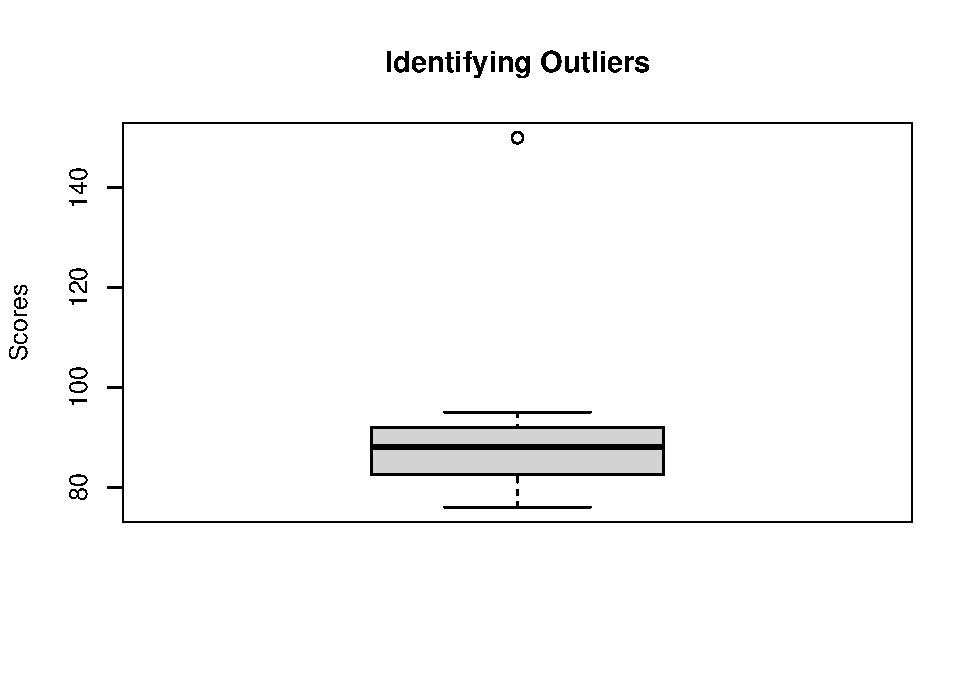
\includegraphics{psych-stats-book_files/figure-latex/unnamed-chunk-15-1.pdf}

\begin{Shaded}
\begin{Highlighting}[]
\CommentTok{\# Calculate the IQR and identify outliers}
\NormalTok{Q1 }\OtherTok{\textless{}{-}} \FunctionTok{quantile}\NormalTok{(scores, }\FloatTok{0.25}\NormalTok{)}
\NormalTok{Q3 }\OtherTok{\textless{}{-}} \FunctionTok{quantile}\NormalTok{(scores, }\FloatTok{0.75}\NormalTok{)}
\NormalTok{IQR }\OtherTok{\textless{}{-}}\NormalTok{ Q3 }\SpecialCharTok{{-}}\NormalTok{ Q1}
\NormalTok{lower\_bound }\OtherTok{\textless{}{-}}\NormalTok{ Q1 }\SpecialCharTok{{-}} \FloatTok{1.5} \SpecialCharTok{*}\NormalTok{ IQR}
\NormalTok{upper\_bound }\OtherTok{\textless{}{-}}\NormalTok{ Q3 }\SpecialCharTok{+} \FloatTok{1.5} \SpecialCharTok{*}\NormalTok{ IQR}
\NormalTok{outliers }\OtherTok{\textless{}{-}}\NormalTok{ scores[scores }\SpecialCharTok{\textless{}}\NormalTok{ lower\_bound }\SpecialCharTok{|}\NormalTok{ scores }\SpecialCharTok{\textgreater{}}\NormalTok{ upper\_bound]}

\FunctionTok{print}\NormalTok{(}\FunctionTok{paste}\NormalTok{(}\StringTok{"Outliers:"}\NormalTok{, }\FunctionTok{paste}\NormalTok{(outliers, }\AttributeTok{collapse =} \StringTok{", "}\NormalTok{)))}
\end{Highlighting}
\end{Shaded}

\begin{verbatim}
## [1] "Outliers: 150"
\end{verbatim}

\hypertarget{handling-outliers}{%
\subsubsection{Handling Outliers}\label{handling-outliers}}

Depending on the context and the research question, outliers can be handled in various ways:

\begin{itemize}
\item
  \textbf{Examine for Errors}: Verify if outliers are due to data entry errors or other mistakes.
\item
  \textbf{Transformation}: Apply transformations (e.g., log transformation) to reduce the impact of outliers.
\item
  \textbf{Robust Statistics}: Use statistical methods that are less affected by outliers, such as the median or trimmed mean.
\item
  \textbf{Separate Analysis}: Analyze outliers separately if they provide valuable insights into a subset of the data.
\end{itemize}

\hypertarget{practical-relevance-1}{%
\subsubsection{Practical Relevance}\label{practical-relevance-1}}

Outliers can provide important information about the variability and distribution of data. However, they can also distort statistical analyses and lead to misleading conclusions if not properly addressed. Understanding and handling outliers appropriately ensures the robustness and validity of research findings.

\hypertarget{conclusion-11}{%
\subsection{Conclusion}\label{conclusion-11}}

Understanding measures of complexity, such as variance and standard deviation, and identifying and handling outliers are critical in psychological research. These measures provide deep insights into data variability, informing the reliability and generalizability of findings. By mastering these concepts and their application in R, researchers can enhance their analytical capabilities and draw more robust conclusions from their data.

\hypertarget{calculating-probabilities}{%
\section{Calculating Probabilities}\label{calculating-probabilities}}

Probability is a fundamental concept in psychological research, allowing researchers to make predictions and decisions based on data. This section provides an overview of probability in the context of psychological research, with a focus on the normal and t-distributions, including how to calculate probabilities and create distribution plots using R.

\hypertarget{overview-of-probability-in-the-context-of-psychological-research}{%
\subsection{Overview of Probability in the Context of Psychological Research}\label{overview-of-probability-in-the-context-of-psychological-research}}

In psychological research, probability helps quantify the likelihood of various outcomes. Understanding probability allows researchers to:

\begin{itemize}
\item
  \textbf{Assess the significance of findings}: Determine whether observed effects are likely due to chance.
\item
  \textbf{Make predictions}: Estimate the likelihood of future events based on current data.
\item
  \textbf{Inform decision-making}: Guide decisions in experimental design, hypothesis testing, and data interpretation.
\end{itemize}

\hypertarget{normal-distribution}{%
\subsection{Normal Distribution}\label{normal-distribution}}

The normal distribution, also known as the Gaussian distribution, is a continuous probability distribution characterized by its bell-shaped curve. It is defined by two parameters: the mean (μ) and the standard deviation (σ). Many psychological variables, such as IQ scores and reaction times, are approximately normally distributed.

\hypertarget{calculating-probabilities-of-scores}{%
\subsubsection{Calculating Probabilities of Scores}\label{calculating-probabilities-of-scores}}

To calculate the probability of a score falling within a certain range in a normal distribution, we use the cumulative distribution function (CDF).

\begin{Shaded}
\begin{Highlighting}[]
\CommentTok{\# Define parameters}
\NormalTok{mean }\OtherTok{\textless{}{-}} \DecValTok{100}
\NormalTok{sd }\OtherTok{\textless{}{-}} \DecValTok{15}

\CommentTok{\# Calculate the probability of a score being less than 110}
\NormalTok{prob\_less\_than\_110 }\OtherTok{\textless{}{-}} \FunctionTok{pnorm}\NormalTok{(}\DecValTok{110}\NormalTok{, mean, sd)}
\FunctionTok{print}\NormalTok{(}\FunctionTok{paste}\NormalTok{(}\StringTok{"Probability of a score less than 110:"}\NormalTok{, prob\_less\_than\_110))}
\end{Highlighting}
\end{Shaded}

\begin{verbatim}
## [1] "Probability of a score less than 110: 0.747507462453077"
\end{verbatim}

\begin{Shaded}
\begin{Highlighting}[]
\CommentTok{\# Calculate the probability of a score between 90 and 110}
\NormalTok{prob\_between\_90\_and\_110 }\OtherTok{\textless{}{-}} \FunctionTok{pnorm}\NormalTok{(}\DecValTok{110}\NormalTok{, mean, sd) }\SpecialCharTok{{-}} \FunctionTok{pnorm}\NormalTok{(}\DecValTok{90}\NormalTok{, mean, sd)}
\FunctionTok{print}\NormalTok{(}\FunctionTok{paste}\NormalTok{(}\StringTok{"Probability of a score between 90 and 110:"}\NormalTok{, prob\_between\_90\_and\_110))}
\end{Highlighting}
\end{Shaded}

\begin{verbatim}
## [1] "Probability of a score between 90 and 110: 0.495014924906154"
\end{verbatim}

Plotting the Normal Distribution in R

\begin{Shaded}
\begin{Highlighting}[]
\CommentTok{\# Generate a sequence of values}
\NormalTok{x }\OtherTok{\textless{}{-}} \FunctionTok{seq}\NormalTok{(mean }\SpecialCharTok{{-}} \DecValTok{4}\SpecialCharTok{*}\NormalTok{sd, mean }\SpecialCharTok{+} \DecValTok{4}\SpecialCharTok{*}\NormalTok{sd, }\AttributeTok{length=}\DecValTok{100}\NormalTok{)}

\CommentTok{\# Calculate the density}
\NormalTok{y }\OtherTok{\textless{}{-}} \FunctionTok{dnorm}\NormalTok{(x, mean, sd)}

\CommentTok{\# Plot the normal distribution}
\FunctionTok{plot}\NormalTok{(x, y, }\AttributeTok{type=}\StringTok{"l"}\NormalTok{, }\AttributeTok{lwd=}\DecValTok{2}\NormalTok{, }\AttributeTok{col=}\StringTok{"blue"}\NormalTok{, }\AttributeTok{main=}\StringTok{"Normal Distribution"}\NormalTok{,}
     \AttributeTok{xlab=}\StringTok{"Scores"}\NormalTok{, }\AttributeTok{ylab=}\StringTok{"Density"}\NormalTok{)}
\end{Highlighting}
\end{Shaded}

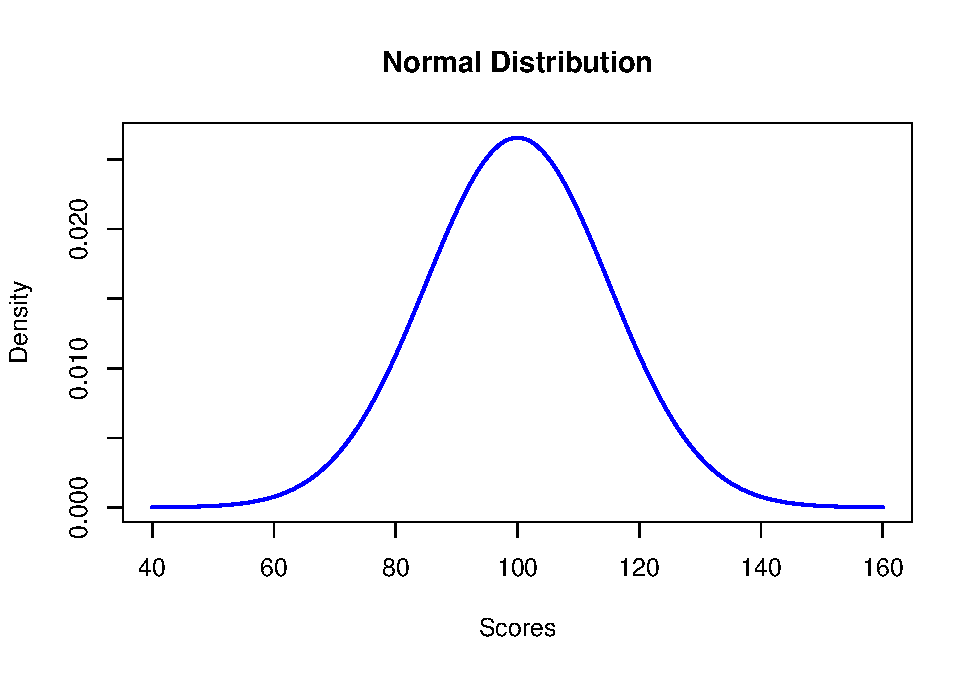
\includegraphics{psych-stats-book_files/figure-latex/unnamed-chunk-17-1.pdf}

\hypertarget{t-distribution}{%
\subsection{T-Distribution}\label{t-distribution}}

The t-distribution is similar to the normal distribution but has thicker tails. It is used instead of the normal distribution when dealing with smaller sample sizes or when the population standard deviation is unknown. The t-distribution is characterized by degrees of freedom (df), which depend on the sample size.

\hypertarget{relevance-and-application-in-smaller-samples}{%
\subsubsection{Relevance and Application in Smaller Samples}\label{relevance-and-application-in-smaller-samples}}

In psychological research, the t-distribution is particularly relevant when:

\begin{itemize}
\item
  \textbf{Sample sizes are small}: The normal distribution may not be an appropriate approximation.
\item
  \textbf{Population standard deviation is unknown}: The t-distribution provides a better estimate of the true distribution.
\end{itemize}

\hypertarget{probability-calculations-in-r}{%
\subsubsection{Probability Calculations in R}\label{probability-calculations-in-r}}

To calculate probabilities using the t-distribution, we use the cumulative distribution function (pt) and the density function (dt).

\begin{Shaded}
\begin{Highlighting}[]
\CommentTok{\# Define parameters}
\NormalTok{df }\OtherTok{\textless{}{-}} \DecValTok{10}  \CommentTok{\# degrees of freedom}

\CommentTok{\# Calculate the probability of a t{-}score being less than 1.5}
\NormalTok{prob\_less\_than\_1\_5 }\OtherTok{\textless{}{-}} \FunctionTok{pt}\NormalTok{(}\FloatTok{1.5}\NormalTok{, df)}
\FunctionTok{print}\NormalTok{(}\FunctionTok{paste}\NormalTok{(}\StringTok{"Probability of a t{-}score less than 1.5:"}\NormalTok{, prob\_less\_than\_1\_5))}
\end{Highlighting}
\end{Shaded}

\begin{verbatim}
## [1] "Probability of a t-score less than 1.5: 0.91774633677728"
\end{verbatim}

\begin{Shaded}
\begin{Highlighting}[]
\CommentTok{\# Calculate the probability of a t{-}score between {-}1 and 1}
\NormalTok{prob\_between\_minus1\_and\_1 }\OtherTok{\textless{}{-}} \FunctionTok{pt}\NormalTok{(}\DecValTok{1}\NormalTok{, df) }\SpecialCharTok{{-}} \FunctionTok{pt}\NormalTok{(}\SpecialCharTok{{-}}\DecValTok{1}\NormalTok{, df)}
\FunctionTok{print}\NormalTok{(}\FunctionTok{paste}\NormalTok{(}\StringTok{"Probability of a t{-}score between {-}1 and 1:"}\NormalTok{, prob\_between\_minus1\_and\_1))}
\end{Highlighting}
\end{Shaded}

\begin{verbatim}
## [1] "Probability of a t-score between -1 and 1: 0.65910686769794"
\end{verbatim}

Plotting the T-Distribution in R

\begin{Shaded}
\begin{Highlighting}[]
\CommentTok{\# Generate a sequence of values}
\NormalTok{x }\OtherTok{\textless{}{-}} \FunctionTok{seq}\NormalTok{(}\SpecialCharTok{{-}}\DecValTok{4}\NormalTok{, }\DecValTok{4}\NormalTok{, }\AttributeTok{length=}\DecValTok{100}\NormalTok{)}

\CommentTok{\# Calculate the density}
\NormalTok{y }\OtherTok{\textless{}{-}} \FunctionTok{dt}\NormalTok{(x, df)}

\CommentTok{\# Plot the t{-}distribution}
\FunctionTok{plot}\NormalTok{(x, y, }\AttributeTok{type=}\StringTok{"l"}\NormalTok{, }\AttributeTok{lwd=}\DecValTok{2}\NormalTok{, }\AttributeTok{col=}\StringTok{"red"}\NormalTok{, }\AttributeTok{main=}\StringTok{"T{-}Distribution"}\NormalTok{,}
     \AttributeTok{xlab=}\StringTok{"T{-}Scores"}\NormalTok{, }\AttributeTok{ylab=}\StringTok{"Density"}\NormalTok{)}
\end{Highlighting}
\end{Shaded}

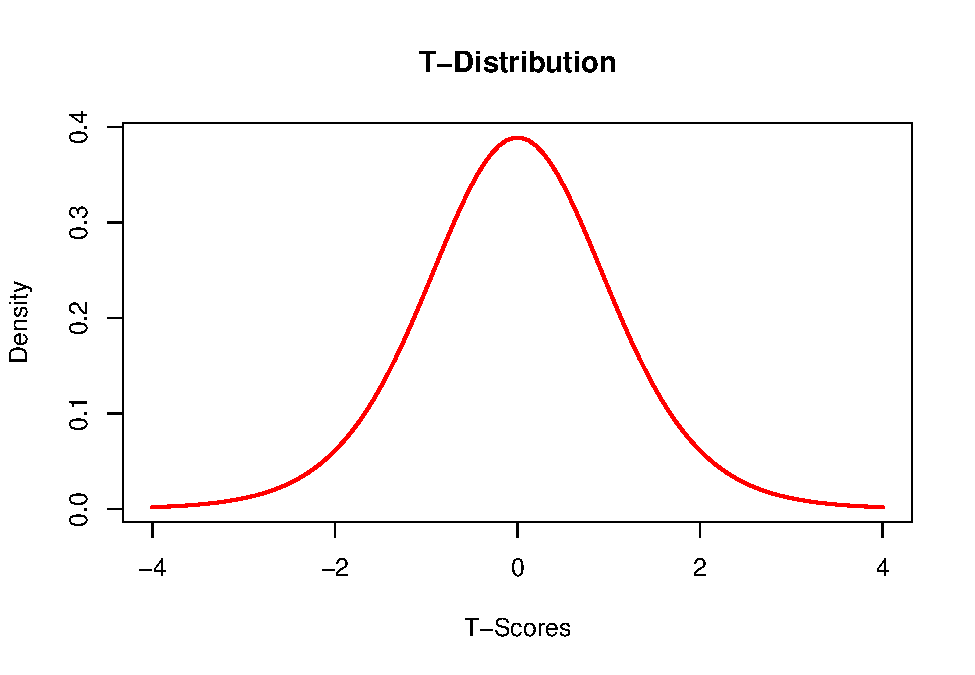
\includegraphics{psych-stats-book_files/figure-latex/unnamed-chunk-19-1.pdf}

\hypertarget{conclusion-12}{%
\subsection{Conclusion}\label{conclusion-12}}

Understanding and calculating probabilities are crucial for making informed decisions and interpretations in psychological research. The normal distribution and t-distribution are foundational concepts that allow researchers to quantify the likelihood of various outcomes and assess the significance of their findings. Using R to perform these calculations and visualizations enhances the ability to apply these statistical concepts effectively in research.

\hypertarget{identifying-a-sample-space}{%
\section{Identifying a Sample Space}\label{identifying-a-sample-space}}

Identifying a sample space is a fundamental concept in probability and statistics. It involves defining all possible outcomes of a random experiment, which is crucial for calculating probabilities and making inferences about a population based on sample data. This section explores the definition and importance of identifying a sample space, along with examples relevant to psychological research.

\hypertarget{definition-and-importance-of-identifying-a-sample-space}{%
\subsection{Definition and Importance of Identifying a Sample Space}\label{definition-and-importance-of-identifying-a-sample-space}}

A \textbf{sample space} is the set of all possible outcomes of a random experiment. In probability theory, it is denoted by the symbol \(S\). Understanding the sample space is essential because:

\begin{enumerate}
\def\labelenumi{\arabic{enumi}.}
\tightlist
\item
  \textbf{Foundation for Probability Calculations}: The sample space provides the basis for calculating probabilities of events. Each outcome in the sample space can be assigned a probability, which helps in determining the likelihood of various events.
\item
  \textbf{Ensuring Completeness}: Defining the sample space ensures that all potential outcomes are considered, preventing the omission of any possibilities that could affect the analysis.
\item
  \textbf{Guiding Data Collection}: A well-defined sample space helps in designing experiments and surveys by clarifying what outcomes need to be observed and recorded.
\item
  \textbf{Facilitating Statistical Inference}: Identifying the sample space is crucial for making inferences about the population based on sample data, as it defines the context in which the data are interpreted.
\end{enumerate}

\hypertarget{examples-of-defining-sample-spaces-for-different-types-of-psychological-data}{%
\subsection{Examples of Defining Sample Spaces for Different Types of Psychological Data}\label{examples-of-defining-sample-spaces-for-different-types-of-psychological-data}}

In psychological research, sample spaces can vary widely depending on the type of data and the nature of the experiment. Below are examples of how to define sample spaces for different types of psychological data.

\hypertarget{example-1-categorical-data}{%
\subsubsection{Example 1: Categorical Data}\label{example-1-categorical-data}}

Consider a survey that asks participants about their preferred type of therapy. The possible responses are: ``Cognitive Behavioral Therapy (CBT)'', ``Psychodynamic Therapy'', ``Humanistic Therapy'', and ``Other''. The sample space \(S\) for this categorical data is: \[ S = \{ \text{CBT}, \text{Psychodynamic}, \text{Humanistic}, \text{Other} \} \]

\hypertarget{example-2-ordinal-data}{%
\subsubsection{Example 2: Ordinal Data}\label{example-2-ordinal-data}}

Imagine a questionnaire that assesses the level of agreement with a statement using a Likert scale with the following options: ``Strongly Disagree'', ``Disagree'', ``Neutral'', ``Agree'', ``Strongly Agree''. The sample space \(S\) for this ordinal data is: \[ S = \{ \text{Strongly Disagree}, \text{Disagree}, \text{Neutral}, \text{Agree}, \text{Strongly Agree} \} \]

\hypertarget{example-3-continuous-data}{%
\subsubsection{Example 3: Continuous Data}\label{example-3-continuous-data}}

Suppose we measure the reaction time (in milliseconds) of participants in a cognitive task. Reaction time is a continuous variable, so the sample space \(S\) is all positive real numbers: \[ S = \{ x \in \mathbb{R} \mid x > 0 \} \]

\hypertarget{example-4-binary-data}{%
\subsubsection{Example 4: Binary Data}\label{example-4-binary-data}}

Consider a simple experiment where participants are asked whether they experienced stress during a task, with responses being either ``Yes'' or ``No''. The sample space \(S\) for this binary data is: \[ S = \{ \text{Yes}, \text{No} \} \]

\hypertarget{practical-example-in-r}{%
\subsection{Practical Example in R}\label{practical-example-in-r}}

Let's illustrate how to define and work with a sample space in R using a simple psychological experiment. Suppose we want to simulate the outcomes of participants reporting their stress levels on a scale from 1 to 5.

\begin{Shaded}
\begin{Highlighting}[]
\CommentTok{\# Define the sample space}
\NormalTok{sample\_space }\OtherTok{\textless{}{-}} \DecValTok{1}\SpecialCharTok{:}\DecValTok{5}

\CommentTok{\# Simulate responses from 100 participants}
\FunctionTok{set.seed}\NormalTok{(}\DecValTok{123}\NormalTok{)  }\CommentTok{\# For reproducibility}
\NormalTok{responses }\OtherTok{\textless{}{-}} \FunctionTok{sample}\NormalTok{(sample\_space, }\DecValTok{100}\NormalTok{, }\AttributeTok{replace =} \ConstantTok{TRUE}\NormalTok{)}

\CommentTok{\# Display the first 10 responses}
\FunctionTok{print}\NormalTok{(responses[}\DecValTok{1}\SpecialCharTok{:}\DecValTok{10}\NormalTok{])}
\end{Highlighting}
\end{Shaded}

\begin{verbatim}
##  [1] 3 3 2 2 3 5 4 1 2 3
\end{verbatim}

This example defines a sample space for stress levels and simulates responses from 100 participants, demonstrating how to work with sample spaces in R.

\hypertarget{conclusion-13}{%
\subsection{Conclusion}\label{conclusion-13}}

Identifying a sample space is a crucial step in probability and statistics, providing the foundation for probability calculations and statistical inference. By defining all possible outcomes, researchers ensure completeness and accuracy in their analyses. Understanding and correctly identifying sample spaces for different types of psychological data enhance the rigor and validity of research findings.

\hypertarget{chapter-summary-3}{%
\section{Chapter Summary}\label{chapter-summary-3}}

Chapter 4 covered key concepts in descriptive statistics and basic probability, essential tools in psychological research for summarizing, interpreting, and making predictions based on data. This chapter highlighted the importance of these statistical methods and provided practical examples using R to illustrate their application.

\hypertarget{key-points-recap-1}{%
\subsection{Key Points Recap}\label{key-points-recap-1}}

\begin{enumerate}
\def\labelenumi{\arabic{enumi}.}
\item
  \textbf{Descriptive Statistics to Summarize Data}:

  \begin{itemize}
  \item
    \textbf{Definition and Importance}: Descriptive statistics help transform raw data into understandable summaries, simplifying data interpretation, identifying trends, and guiding further analysis.
  \item
    \textbf{Measures of Centrality}:

    \begin{itemize}
    \item
      \textbf{Mean}: The average value, useful for symmetrically distributed data without outliers.
    \item
      \textbf{Median}: The middle value, ideal for skewed distributions and data with outliers.
    \item
      \textbf{Mode}: The most frequently occurring value, important for nominal data and multimodal distributions.
    \end{itemize}
  \item
    \textbf{Measures of Complexity}:

    \begin{itemize}
    \item
      \textbf{Range}: The difference between the highest and lowest values, providing a quick sense of data spread.
    \item
      \textbf{Variance}: Measures the average degree of deviation from the mean, highlighting data variability.
    \item
      \textbf{Standard Deviation}: The square root of variance, expressed in the same units as the data, making it more interpretable and practical for comparing data sets.
    \item
      \textbf{Outliers}: Identifying and handling outliers to ensure robust statistical analyses.
    \end{itemize}
  \end{itemize}
\item
  \textbf{Calculating Probabilities}:

  \begin{itemize}
  \item
    \textbf{Overview of Probability}: Probability quantifies the likelihood of various outcomes, essential for hypothesis testing, predictions, and decision-making in psychological research.
  \item
    \textbf{Normal Distribution}: Characterized by its bell-shaped curve, used to calculate probabilities and visualize data distribution.

    \begin{itemize}
    \tightlist
    \item
      Practical examples in R to calculate probabilities and plot the normal distribution.
    \end{itemize}
  \item
    \textbf{T-Distribution}: Similar to the normal distribution but with thicker tails, relevant for smaller samples and unknown population standard deviations.

    \begin{itemize}
    \tightlist
    \item
      Practical examples in R to calculate probabilities and plot the t-distribution.
    \end{itemize}
  \end{itemize}
\item
  \textbf{Identifying a Sample Space}:

  \begin{itemize}
  \item
    \textbf{Definition and Importance}: A sample space is the set of all possible outcomes of a random experiment, forming the foundation for probability calculations and ensuring completeness in data analysis.
  \item
    \textbf{Examples}: Defining sample spaces for different types of psychological data (categorical, ordinal, continuous, binary) and practical R examples to illustrate their application.
  \end{itemize}
\end{enumerate}

\hypertarget{practical-applications}{%
\subsection{Practical Applications}\label{practical-applications}}

Throughout the chapter, practical R examples demonstrated how to compute descriptive statistics, calculate probabilities, and define sample spaces. These hands-on exercises are designed to enhance your ability to apply statistical concepts in psychological research effectively.

\hypertarget{conclusion-14}{%
\subsection{Conclusion}\label{conclusion-14}}

Understanding and applying descriptive statistics and probability concepts are fundamental skills in psychological research. These tools enable researchers to summarize complex data, make informed decisions, and draw reliable conclusions. By mastering these concepts and their practical implementation in R, you can significantly improve the rigor and validity of your research findings.

This chapter provided a comprehensive overview of these essential statistical methods, preparing you for more advanced analyses and applications in subsequent chapters.

\hypertarget{practice-exercises-2}{%
\section{Practice Exercises}\label{practice-exercises-2}}

These exercises aim to test your understanding of descriptive statistics and probability, encouraging the application of concepts learned in Chapter 4 to practical problems using R.

\hypertarget{exercise-1-calculating-descriptive-statistics}{%
\subsection{Exercise 1: Calculating Descriptive Statistics}\label{exercise-1-calculating-descriptive-statistics}}

\begin{itemize}
\item
  \textbf{Task}: Given a dataset of test scores, calculate the mean, median, mode, variance, and standard deviation. Identify any outliers in the dataset.
\item
  \textbf{Dataset}: Use the following scores for the analysis: \texttt{c(55,\ 65,\ 75,\ 85,\ 95,\ 105,\ 115,\ 125,\ 135,\ 145)}.
\item
  \textbf{Questions}: Write the R code to perform these calculations and interpret the results.
\end{itemize}

\hypertarget{exercise-2-understanding-the-normal-distribution}{%
\subsection{Exercise 2: Understanding the Normal Distribution}\label{exercise-2-understanding-the-normal-distribution}}

\begin{itemize}
\item
  \textbf{Task}: Assume a psychological test follows a normal distribution with a mean of 100 and a standard deviation of 15. Calculate the probability that a randomly selected individual scores:

  \begin{itemize}
  \item
    \begin{enumerate}
    \def\labelenumi{\alph{enumi})}
    \tightlist
    \item
      Less than 85
    \end{enumerate}
  \item
    \begin{enumerate}
    \def\labelenumi{\alph{enumi})}
    \setcounter{enumi}{1}
    \tightlist
    \item
      Between 85 and 115
    \end{enumerate}
  \end{itemize}
\item
  \textbf{Questions}: Use R to find these probabilities and explain the significance of your findings.
\end{itemize}

\hypertarget{exercise-3-applying-the-t-distribution}{%
\subsection{Exercise 3: Applying the T-Distribution}\label{exercise-3-applying-the-t-distribution}}

\begin{itemize}
\item
  \textbf{Task}: You are conducting a small-scale study with 12 participants. Calculate the probability of a t-score being less than 1.5 and between -1 and 1 using the t-distribution.
\item
  \textbf{Questions}: Write the R code for these calculations and discuss how the results might differ if a normal distribution were assumed.
\end{itemize}

\hypertarget{exercise-4-defining-and-simulating-sample-spaces}{%
\subsection{Exercise 4: Defining and Simulating Sample Spaces}\label{exercise-4-defining-and-simulating-sample-spaces}}

\begin{itemize}
\item
  \textbf{Task}: Define a sample space for a study where participants can choose between three types of exercises (Yoga, Pilates, Aerobics). Simulate responses from 100 participants.
\item
  \textbf{Questions}: Define the sample space, simulate the responses using R, and analyze the frequency of each exercise choice.
\end{itemize}

\hypertarget{computation}{%
\chapter{Computation}\label{computation}}

\hypertarget{overview-of-the-importance-of-data-computation-and-manipulation-in-psychological-research}{%
\section{Overview of the Importance of Data Computation and Manipulation in Psychological Research}\label{overview-of-the-importance-of-data-computation-and-manipulation-in-psychological-research}}

In psychological research, data computation and manipulation are crucial steps that transform raw data into meaningful information. These processes allow researchers to clean, organize, and analyze data effectively, leading to more accurate and reliable conclusions.

\hypertarget{importance-of-data-computation-and-manipulation}{%
\section{Importance of Data Computation and Manipulation}\label{importance-of-data-computation-and-manipulation}}

\begin{enumerate}
\def\labelenumi{\arabic{enumi}.}
\item
  \textbf{Data Cleaning}:

  \begin{itemize}
  \item
    Ensures the accuracy and consistency of data.
  \item
    Involves identifying and correcting errors, handling missing values, and removing outliers.
  \item
    Prevents erroneous results that can arise from flawed data.
  \end{itemize}
\item
  \textbf{Data Organization}:

  \begin{itemize}
  \item
    Facilitates easier analysis and interpretation.
  \item
    Involves structuring data in a logical format, such as tidy data principles where each variable forms a column and each observation forms a row.
  \item
    Enhances the readability and usability of the dataset.
  \end{itemize}
\item
  \textbf{Data Transformation}:

  \begin{itemize}
  \item
    Involves converting data into a suitable format for analysis.
  \item
    Includes normalization, aggregation, and creating new variables.
  \item
    Enables the application of various statistical techniques and models.
  \end{itemize}
\item
  \textbf{Data Exploration}:

  \begin{itemize}
  \item
    Provides insights into data distributions, relationships, and patterns.
  \item
    Utilizes descriptive statistics and visualization techniques.
  \item
    Helps in forming hypotheses and guiding further analysis.
  \end{itemize}
\item
  \textbf{Ensuring Reproducibility}:

  \begin{itemize}
  \item
    Essential for validating and replicating research findings.
  \item
    Involves documenting and sharing data manipulation steps and analysis scripts.
  \item
    Enhances transparency and credibility of the research.
  \end{itemize}
\end{enumerate}

By systematically computing and manipulating data, psychological researchers can ensure the integrity of their data, leading to more robust and credible research outcomes.

\hypertarget{brief-introduction-to-rs-capabilities-for-data-handling}{%
\section{Brief Introduction to R's Capabilities for Data Handling}\label{brief-introduction-to-rs-capabilities-for-data-handling}}

R is a powerful statistical programming language widely used in psychological research for data handling, analysis, and visualization. Its extensive package ecosystem and versatile functions make it an ideal tool for various data manipulation tasks.

\hypertarget{key-capabilities-of-r-for-data-handling}{%
\subsection{Key Capabilities of R for Data Handling}\label{key-capabilities-of-r-for-data-handling}}

\begin{enumerate}
\def\labelenumi{\arabic{enumi}.}
\item
  \textbf{Data Importation}:

  \begin{itemize}
  \item
    R can import data from various sources, including CSV files, Excel files, databases, and web APIs.
  \item
    Functions such as \texttt{read.csv()}, \texttt{read\_excel()}, and \texttt{dbConnect()} facilitate data importation.
  \end{itemize}
\item
  \textbf{Data Cleaning}:

  \begin{itemize}
  \item
    R provides functions to handle missing values (\texttt{na.omit()}, \texttt{is.na()}), detect and remove outliers, and correct data entry errors.
  \item
    The \texttt{dplyr} package offers a range of functions (\texttt{mutate()}, \texttt{filter()}, \texttt{select()}, \texttt{rename()}) for efficient data cleaning.
  \end{itemize}
\item
  \textbf{Data Transformation}:

  \begin{itemize}
  \item
    R allows for data transformation through functions like \texttt{mutate()} for creating new variables, \texttt{summarize()} for aggregation, and \texttt{spread()}/\texttt{gather()} for reshaping data.
  \item
    The \texttt{tidyverse} package is particularly useful for data transformation tasks.
  \end{itemize}
\item
  \textbf{Data Visualization}:

  \begin{itemize}
  \item
    R supports various visualization techniques through packages like \texttt{ggplot2}, \texttt{lattice}, and \texttt{plotly}.
  \item
    These packages enable the creation of informative plots such as histograms, scatter plots, and boxplots.
  \end{itemize}
\item
  \textbf{Statistical Analysis}:

  \begin{itemize}
  \item
    R is equipped with numerous statistical functions and models, including t-tests, ANOVA, regression analysis, and more.
  \item
    The \texttt{stats} package provides foundational statistical functions, while specialized packages like \texttt{psych} offer additional tools for psychological research.
  \end{itemize}
\item
  \textbf{Reproducibility}:

  \begin{itemize}
  \item
    RMarkdown and \texttt{knitr} allow for the creation of dynamic documents that integrate code, output, and narrative text.
  \item
    These tools facilitate reproducible research by enabling researchers to document and share their analysis workflows.
  \end{itemize}
\end{enumerate}

\hypertarget{importing-data-from-excel-files}{%
\section{Importing Data from Excel Files}\label{importing-data-from-excel-files}}

In psychological research, data is often stored in Excel files, either in CSV (.csv) format or Excel Workbook (.xlsx) format. Importing this data into R is a crucial first step in data analysis. This section covers the process of importing data from both .csv and .xlsx files using R.

\hypertarget{importing-.csv-files}{%
\subsection{Importing .csv Files}\label{importing-.csv-files}}

CSV (Comma-Separated Values) files are a common format for storing tabular data. They are simple text files where each line represents a row in the table, and columns are separated by commas.

\hypertarget{step-by-step-guide-to-importing-.csv-files}{%
\subsubsection{Step-by-Step Guide to Importing .csv Files}\label{step-by-step-guide-to-importing-.csv-files}}

\begin{enumerate}
\def\labelenumi{\arabic{enumi}.}
\item
  \textbf{Prepare the CSV File}: Ensure the CSV file is properly formatted with a header row containing column names.
\item
  \textbf{Set the Working Directory}: Set the working directory in R to the location of the CSV file.
\item
  \textbf{Use \texttt{read.csv()} Function}: Use the \texttt{read.csv()} function to read the data into R.
\end{enumerate}

\begin{Shaded}
\begin{Highlighting}[]
\CommentTok{\# Set the working directory to the location of your CSV file}
\FunctionTok{setwd}\NormalTok{(}\StringTok{"path/to/your/folder"}\NormalTok{)}

\CommentTok{\# Import the CSV file}
\NormalTok{data\_csv }\OtherTok{\textless{}{-}} \FunctionTok{read.csv}\NormalTok{(}\StringTok{"your\_file.csv"}\NormalTok{)}

\CommentTok{\# View the first few rows of the data}
\FunctionTok{head}\NormalTok{(data\_csv)}
\end{Highlighting}
\end{Shaded}

Suppose you have a CSV file named ``study\_data.csv'' containing participant responses to a psychological survey.

\begin{Shaded}
\begin{Highlighting}[]
\CommentTok{\# Set the working directory}
\FunctionTok{setwd}\NormalTok{(}\StringTok{"path/to/your/folder"}\NormalTok{)}

\CommentTok{\# Import the CSV file}
\NormalTok{study\_data }\OtherTok{\textless{}{-}} \FunctionTok{read.csv}\NormalTok{(}\StringTok{"study\_data.csv"}\NormalTok{)}

\CommentTok{\# View the first few rows of the data}
\FunctionTok{head}\NormalTok{(study\_data)}
\end{Highlighting}
\end{Shaded}

This code sets the working directory, imports the CSV file, and displays the first few rows of the dataset.

\hypertarget{importing-.xlsx-files}{%
\subsection{Importing .xlsx Files}\label{importing-.xlsx-files}}

Excel Workbook (.xlsx) files are another common format for storing data. They can contain multiple sheets and more complex formatting than CSV files. The \texttt{readxl} package in R allows for easy import of .xlsx files.

\hypertarget{step-by-step-guide-to-importing-.xlsx-files}{%
\subsubsection{Step-by-Step Guide to Importing .xlsx Files}\label{step-by-step-guide-to-importing-.xlsx-files}}

\begin{enumerate}
\def\labelenumi{\arabic{enumi}.}
\item
  \textbf{Install and Load the \texttt{readxl} Package}: If you haven't already installed the \texttt{readxl} package, you can do so using \texttt{install.packages()}.
\item
  \textbf{Use \texttt{read\_excel()} Function}: Use the \texttt{read\_excel()} function to read the data from the Excel file.
\end{enumerate}

\begin{Shaded}
\begin{Highlighting}[]
\CommentTok{\# Install the readxl package (if not already installed)}
\FunctionTok{install.packages}\NormalTok{(}\StringTok{"readxl"}\NormalTok{)}

\CommentTok{\# Load the readxl package}
\FunctionTok{library}\NormalTok{(readxl)}

\CommentTok{\# Import the Excel file}
\NormalTok{data\_xlsx }\OtherTok{\textless{}{-}} \FunctionTok{read\_excel}\NormalTok{(}\StringTok{"path/to/your/file.xlsx"}\NormalTok{)}

\CommentTok{\# View the first few rows of the data}
\FunctionTok{head}\NormalTok{(data\_xlsx)}
\end{Highlighting}
\end{Shaded}

Suppose you have an Excel file named ``experiment\_data.xlsx'' with multiple sheets. You can specify the sheet to read from using the sheet argument.

\begin{Shaded}
\begin{Highlighting}[]
\CommentTok{\# Load the readxl package}
\FunctionTok{library}\NormalTok{(readxl)}

\CommentTok{\# Import the Excel file, reading from the first sheet by default}
\NormalTok{experiment\_data }\OtherTok{\textless{}{-}} \FunctionTok{read\_excel}\NormalTok{(}\StringTok{"experiment\_data.xlsx"}\NormalTok{)}

\CommentTok{\# View the first few rows of the data}
\FunctionTok{head}\NormalTok{(experiment\_data)}

\CommentTok{\# Import data from a specific sheet}
\NormalTok{experiment\_data\_sheet2 }\OtherTok{\textless{}{-}} \FunctionTok{read\_excel}\NormalTok{(}\StringTok{"experiment\_data.xlsx"}\NormalTok{, }\AttributeTok{sheet =} \StringTok{"Sheet2"}\NormalTok{)}

\CommentTok{\# View the first few rows of the data from Sheet2}
\FunctionTok{head}\NormalTok{(experiment\_data\_sheet2)}
\end{Highlighting}
\end{Shaded}

This code demonstrates how to import data from an Excel file and how to read data from a specific sheet within the file.

\hypertarget{conclusion-15}{%
\subsection{Conclusion}\label{conclusion-15}}

Importing data from Excel files into R is a fundamental step in data analysis. Whether dealing with simple CSV files or complex Excel Workbooks, R provides powerful functions to efficiently read and handle this data. In the next section, we will explore techniques for cleaning the imported data to ensure its accuracy and readiness for analysis.

\hypertarget{cleaning-data}{%
\section{Cleaning Data}\label{cleaning-data}}

Cleaning data is a crucial step in the data analysis process, ensuring that your data is accurate, consistent, and ready for analysis. The \texttt{dplyr} package in R provides a powerful and intuitive set of functions for data manipulation, making it easier to clean and prepare your data.

\hypertarget{introduction-to-dplyr}{%
\subsection{\texorpdfstring{Introduction to \texttt{dplyr}}{Introduction to dplyr}}\label{introduction-to-dplyr}}

\texttt{dplyr} is part of the tidyverse, a collection of R packages designed for data science. It provides a set of functions that are specifically designed for data manipulation tasks, including filtering, selecting, mutating, summarizing, arranging data, removing outliers, and releveling categorical factors.

\hypertarget{installing-and-loading-dplyr}{%
\subsubsection{\texorpdfstring{Installing and Loading \texttt{dplyr}}{Installing and Loading dplyr}}\label{installing-and-loading-dplyr}}

\begin{Shaded}
\begin{Highlighting}[]
\CommentTok{\# Install the dplyr package (if not already installed)}
\ControlFlowTok{if}\NormalTok{(}\SpecialCharTok{!}\FunctionTok{require}\NormalTok{(dplyr))\{}\FunctionTok{install.packages}\NormalTok{(}\StringTok{"dplyr"}\NormalTok{, }\AttributeTok{dependencies=}\ConstantTok{TRUE}\NormalTok{)\}}
\end{Highlighting}
\end{Shaded}

\begin{verbatim}
## Loading required package: dplyr
\end{verbatim}

\begin{verbatim}
## Warning: package 'dplyr' was built under R version 4.3.3
\end{verbatim}

\begin{verbatim}
## 
## Attaching package: 'dplyr'
\end{verbatim}

\begin{verbatim}
## The following objects are masked from 'package:stats':
## 
##     filter, lag
\end{verbatim}

\begin{verbatim}
## The following objects are masked from 'package:base':
## 
##     intersect, setdiff, setequal, union
\end{verbatim}

\begin{Shaded}
\begin{Highlighting}[]
\CommentTok{\# Load the dplyr package}
\FunctionTok{library}\NormalTok{(dplyr)}
\end{Highlighting}
\end{Shaded}

\hypertarget{key-dplyr-functions-for-data-cleaning}{%
\subsection{\texorpdfstring{Key \texttt{dplyr} Functions for Data Cleaning}{Key dplyr Functions for Data Cleaning}}\label{key-dplyr-functions-for-data-cleaning}}

\begin{enumerate}
\def\labelenumi{\arabic{enumi}.}
\item
  \textbf{\texttt{filter()}}: Subset rows based on conditions.
\item
  \textbf{\texttt{select()}}: Select columns by name.
\item
  \textbf{\texttt{rename()}}: Rename columns.
\item
  \textbf{\texttt{mutate()}}: Create new columns or modify existing ones.
\item
  \textbf{\texttt{arrange()}}: Arrange rows by column values.
\item
  \textbf{\texttt{summarize()}}: Summarize multiple values to a single value.
\item
  \textbf{\texttt{group\_by()}}: Group data by one or more variables.
\item
  \textbf{\texttt{remove\_outliers()}}: Custom function to remove outliers.
\item
  \textbf{\texttt{relevel()}}: Relevel categorical factors for meaningful analysis.
\end{enumerate}

\hypertarget{filter-subsetting-rows}{%
\subsubsection{\texorpdfstring{1. \texttt{filter()}: Subsetting Rows}{1. filter(): Subsetting Rows}}\label{filter-subsetting-rows}}

The \texttt{filter()} function is used to subset rows based on one or more conditions.

\textbf{Example}: Filter rows where the age is greater than 30.

\begin{Shaded}
\begin{Highlighting}[]
\CommentTok{\# Sample data}
\NormalTok{data }\OtherTok{\textless{}{-}} \FunctionTok{data.frame}\NormalTok{(}
  \AttributeTok{id =} \DecValTok{1}\SpecialCharTok{:}\DecValTok{10}\NormalTok{,}
  \AttributeTok{age =} \FunctionTok{c}\NormalTok{(}\DecValTok{23}\NormalTok{, }\DecValTok{35}\NormalTok{, }\DecValTok{42}\NormalTok{, }\DecValTok{28}\NormalTok{, }\DecValTok{30}\NormalTok{, }\DecValTok{34}\NormalTok{, }\DecValTok{21}\NormalTok{, }\DecValTok{40}\NormalTok{, }\DecValTok{29}\NormalTok{, }\DecValTok{31}\NormalTok{)}
\NormalTok{)}

\CommentTok{\# Filter rows where age is greater than 30}
\NormalTok{filtered\_data }\OtherTok{\textless{}{-}}\NormalTok{ data }\SpecialCharTok{\%\textgreater{}\%}
  \FunctionTok{filter}\NormalTok{(age }\SpecialCharTok{\textgreater{}} \DecValTok{30}\NormalTok{)}

\FunctionTok{print}\NormalTok{(filtered\_data)}
\end{Highlighting}
\end{Shaded}

\begin{verbatim}
##   id age
## 1  2  35
## 2  3  42
## 3  6  34
## 4  8  40
## 5 10  31
\end{verbatim}

\hypertarget{select-selecting-columns}{%
\subsubsection{\texorpdfstring{2. \texttt{select()}: Selecting Columns}{2. select(): Selecting Columns}}\label{select-selecting-columns}}

The \texttt{select()} function is used to select specific columns from a dataset.

\textbf{Example}: Select the id and age columns.

\begin{Shaded}
\begin{Highlighting}[]
\CommentTok{\# Select id and age columns}
\NormalTok{selected\_data }\OtherTok{\textless{}{-}}\NormalTok{ data }\SpecialCharTok{\%\textgreater{}\%}
  \FunctionTok{select}\NormalTok{(id, age)}

\FunctionTok{print}\NormalTok{(selected\_data)}
\end{Highlighting}
\end{Shaded}

\begin{verbatim}
##    id age
## 1   1  23
## 2   2  35
## 3   3  42
## 4   4  28
## 5   5  30
## 6   6  34
## 7   7  21
## 8   8  40
## 9   9  29
## 10 10  31
\end{verbatim}

\hypertarget{rename-renaming-columns}{%
\subsubsection{\texorpdfstring{3. \texttt{rename()}: Renaming Columns}{3. rename(): Renaming Columns}}\label{rename-renaming-columns}}

The \texttt{rename()} function is used to rename columns in a dataset.

\textbf{Example}: Rename the column \texttt{age} to \texttt{participant\_age}.

\begin{Shaded}
\begin{Highlighting}[]
\CommentTok{\# Rename age to participant\_age}
\NormalTok{renamed\_data }\OtherTok{\textless{}{-}}\NormalTok{ data }\SpecialCharTok{\%\textgreater{}\%}
  \FunctionTok{rename}\NormalTok{(}\AttributeTok{participant\_age =}\NormalTok{ age)}

\FunctionTok{print}\NormalTok{(renamed\_data)}
\end{Highlighting}
\end{Shaded}

\begin{verbatim}
##    id participant_age
## 1   1              23
## 2   2              35
## 3   3              42
## 4   4              28
## 5   5              30
## 6   6              34
## 7   7              21
## 8   8              40
## 9   9              29
## 10 10              31
\end{verbatim}

\hypertarget{mutate-creating-or-modifying-columns}{%
\subsubsection{\texorpdfstring{4. \texttt{mutate()}: Creating or Modifying Columns}{4. mutate(): Creating or Modifying Columns}}\label{mutate-creating-or-modifying-columns}}

The \texttt{mutate()} function is used to create new columns or modify existing ones.

\textbf{Example}: Create a new column \texttt{age\_group} based on the age.

\begin{Shaded}
\begin{Highlighting}[]
\CommentTok{\# Create a new column age\_group}
\NormalTok{mutated\_data }\OtherTok{\textless{}{-}}\NormalTok{ data }\SpecialCharTok{\%\textgreater{}\%}
  \FunctionTok{mutate}\NormalTok{(}\AttributeTok{age\_group =} \FunctionTok{ifelse}\NormalTok{(age }\SpecialCharTok{\textgreater{}} \DecValTok{30}\NormalTok{, }\StringTok{"Above 30"}\NormalTok{, }\StringTok{"30 or Below"}\NormalTok{))}

\FunctionTok{print}\NormalTok{(mutated\_data)}
\end{Highlighting}
\end{Shaded}

\begin{verbatim}
##    id age   age_group
## 1   1  23 30 or Below
## 2   2  35    Above 30
## 3   3  42    Above 30
## 4   4  28 30 or Below
## 5   5  30 30 or Below
## 6   6  34    Above 30
## 7   7  21 30 or Below
## 8   8  40    Above 30
## 9   9  29 30 or Below
## 10 10  31    Above 30
\end{verbatim}

\hypertarget{arrange-arranging-rows}{%
\subsubsection{\texorpdfstring{5. \texttt{arrange()}: Arranging Rows}{5. arrange(): Arranging Rows}}\label{arrange-arranging-rows}}

The \texttt{arrange()} function is used to sort rows by column values.

\textbf{Example}: Arrange rows by age in descending order.

\begin{Shaded}
\begin{Highlighting}[]
\CommentTok{\# Arrange rows by age in descending order}
\NormalTok{arranged\_data }\OtherTok{\textless{}{-}}\NormalTok{ data }\SpecialCharTok{\%\textgreater{}\%}
  \FunctionTok{arrange}\NormalTok{(}\FunctionTok{desc}\NormalTok{(age))}

\FunctionTok{print}\NormalTok{(arranged\_data)}
\end{Highlighting}
\end{Shaded}

\begin{verbatim}
##    id age
## 1   3  42
## 2   8  40
## 3   2  35
## 4   6  34
## 5  10  31
## 6   5  30
## 7   9  29
## 8   4  28
## 9   1  23
## 10  7  21
\end{verbatim}

\hypertarget{summarize-summarizing-values}{%
\subsubsection{\texorpdfstring{6. \texttt{summarize()}: Summarizing Values}{6. summarize(): Summarizing Values}}\label{summarize-summarizing-values}}

The \texttt{summarize()} function is used to summarize multiple values into a single value.

\textbf{Example}: Calculate the average age.

\begin{Shaded}
\begin{Highlighting}[]
\CommentTok{\# Calculate the average age}
\NormalTok{summary\_data }\OtherTok{\textless{}{-}}\NormalTok{ data }\SpecialCharTok{\%\textgreater{}\%}
  \FunctionTok{summarize}\NormalTok{(}\AttributeTok{average\_age =} \FunctionTok{mean}\NormalTok{(age))}

\FunctionTok{print}\NormalTok{(summary\_data)}
\end{Highlighting}
\end{Shaded}

\begin{verbatim}
##   average_age
## 1        31.3
\end{verbatim}

\hypertarget{group_by-grouping-data}{%
\subsubsection{\texorpdfstring{7. \texttt{group\_by()}: Grouping Data}{7. group\_by(): Grouping Data}}\label{group_by-grouping-data}}

The \texttt{group\_by()} function is used to group data by one or more variables, often used in conjunction with \texttt{summarize()}.

\textbf{Example}: Group data by \texttt{age\_group} and calculate the average age for each group.

\begin{Shaded}
\begin{Highlighting}[]
\CommentTok{\# Group by age\_group and calculate average age for each group}
\NormalTok{grouped\_data }\OtherTok{\textless{}{-}}\NormalTok{ mutated\_data }\SpecialCharTok{\%\textgreater{}\%}
  \FunctionTok{group\_by}\NormalTok{(age\_group) }\SpecialCharTok{\%\textgreater{}\%}
  \FunctionTok{summarize}\NormalTok{(}\AttributeTok{average\_age =} \FunctionTok{mean}\NormalTok{(age))}

\FunctionTok{print}\NormalTok{(grouped\_data)}
\end{Highlighting}
\end{Shaded}

\begin{verbatim}
## # A tibble: 2 x 2
##   age_group   average_age
##   <chr>             <dbl>
## 1 30 or Below        26.2
## 2 Above 30           36.4
\end{verbatim}

\hypertarget{removing-outliers}{%
\subsubsection{8. Removing Outliers}\label{removing-outliers}}

Outliers can skew your analysis and lead to misleading results. Removing outliers helps in obtaining a more accurate representation of the data.

\textbf{Example}: Removing outliers based on the IQR method.

\begin{Shaded}
\begin{Highlighting}[]
\CommentTok{\# Custom function to remove outliers}
\NormalTok{remove\_outliers }\OtherTok{\textless{}{-}} \ControlFlowTok{function}\NormalTok{(data, column) \{}
\NormalTok{  Q1 }\OtherTok{\textless{}{-}} \FunctionTok{quantile}\NormalTok{(data[[column]], }\FloatTok{0.25}\NormalTok{)}
\NormalTok{  Q3 }\OtherTok{\textless{}{-}} \FunctionTok{quantile}\NormalTok{(data[[column]], }\FloatTok{0.75}\NormalTok{)}
\NormalTok{  IQR }\OtherTok{\textless{}{-}}\NormalTok{ Q3 }\SpecialCharTok{{-}}\NormalTok{ Q1}
\NormalTok{  lower\_bound }\OtherTok{\textless{}{-}}\NormalTok{ Q1 }\SpecialCharTok{{-}} \FloatTok{1.5} \SpecialCharTok{*}\NormalTok{ IQR}
\NormalTok{  upper\_bound }\OtherTok{\textless{}{-}}\NormalTok{ Q3 }\SpecialCharTok{+} \FloatTok{1.5} \SpecialCharTok{*}\NormalTok{ IQR}
\NormalTok{  data }\OtherTok{\textless{}{-}}\NormalTok{ data }\SpecialCharTok{\%\textgreater{}\%}
    \FunctionTok{filter}\NormalTok{(data[[column]] }\SpecialCharTok{\textgreater{}=}\NormalTok{ lower\_bound }\SpecialCharTok{\&}\NormalTok{ data[[column]] }\SpecialCharTok{\textless{}=}\NormalTok{ upper\_bound)}
  \FunctionTok{return}\NormalTok{(data)}
\NormalTok{\}}

\CommentTok{\# Remove outliers from the age column}
\NormalTok{data\_no\_outliers }\OtherTok{\textless{}{-}} \FunctionTok{remove\_outliers}\NormalTok{(data, }\StringTok{"age"}\NormalTok{)}

\FunctionTok{print}\NormalTok{(data\_no\_outliers)}
\end{Highlighting}
\end{Shaded}

\begin{verbatim}
##    id age
## 1   1  23
## 2   2  35
## 3   3  42
## 4   4  28
## 5   5  30
## 6   6  34
## 7   7  21
## 8   8  40
## 9   9  29
## 10 10  31
\end{verbatim}

\hypertarget{releveling-categorical-factors}{%
\subsubsection{9. Releveling Categorical Factors}\label{releveling-categorical-factors}}

Releveling categorical factors ensures that the reference level is meaningful for your analysis. This is particularly important in regression models where the reference level serves as the baseline.

\textbf{Example}: Relevel the \texttt{age\_group} column to set ``30 or Below'' as the reference level.

\begin{Shaded}
\begin{Highlighting}[]
\CommentTok{\# Relevel age\_group to set "30 or Below" as the reference level}
\NormalTok{mutated\_data }\OtherTok{\textless{}{-}}\NormalTok{ mutated\_data }\SpecialCharTok{\%\textgreater{}\%}
  \FunctionTok{mutate}\NormalTok{(}\AttributeTok{age\_group =} \FunctionTok{relevel}\NormalTok{(}\FunctionTok{factor}\NormalTok{(age\_group), }\AttributeTok{ref =} \StringTok{"30 or Below"}\NormalTok{))}

\FunctionTok{print}\NormalTok{(mutated\_data)}
\end{Highlighting}
\end{Shaded}

\begin{verbatim}
##    id age   age_group
## 1   1  23 30 or Below
## 2   2  35    Above 30
## 3   3  42    Above 30
## 4   4  28 30 or Below
## 5   5  30 30 or Below
## 6   6  34    Above 30
## 7   7  21 30 or Below
## 8   8  40    Above 30
## 9   9  29 30 or Below
## 10 10  31    Above 30
\end{verbatim}

\hypertarget{practical-examples-of-data-cleaning}{%
\subsection{Practical Examples of Data Cleaning}\label{practical-examples-of-data-cleaning}}

Combining multiple \texttt{dplyr} functions can make complex data cleaning tasks straightforward.

\textbf{Example 1}: Cleaning a Survey Dataset

\begin{Shaded}
\begin{Highlighting}[]
\CommentTok{\# Sample survey data}
\NormalTok{survey\_data }\OtherTok{\textless{}{-}} \FunctionTok{data.frame}\NormalTok{(}
  \AttributeTok{id =} \DecValTok{1}\SpecialCharTok{:}\DecValTok{10}\NormalTok{,}
  \AttributeTok{age =} \FunctionTok{c}\NormalTok{(}\DecValTok{23}\NormalTok{, }\DecValTok{35}\NormalTok{, }\DecValTok{42}\NormalTok{, }\ConstantTok{NA}\NormalTok{, }\DecValTok{30}\NormalTok{, }\DecValTok{34}\NormalTok{, }\DecValTok{21}\NormalTok{, }\DecValTok{40}\NormalTok{, }\DecValTok{29}\NormalTok{, }\DecValTok{31}\NormalTok{),}
  \AttributeTok{gender =} \FunctionTok{c}\NormalTok{(}\StringTok{"M"}\NormalTok{, }\StringTok{"F"}\NormalTok{, }\StringTok{"F"}\NormalTok{, }\StringTok{"M"}\NormalTok{, }\StringTok{"M"}\NormalTok{, }\StringTok{"F"}\NormalTok{, }\StringTok{"M"}\NormalTok{, }\StringTok{"F"}\NormalTok{, }\StringTok{"M"}\NormalTok{, }\StringTok{"F"}\NormalTok{),}
  \AttributeTok{score =} \FunctionTok{c}\NormalTok{(}\DecValTok{80}\NormalTok{, }\DecValTok{85}\NormalTok{, }\DecValTok{78}\NormalTok{, }\DecValTok{90}\NormalTok{, }\DecValTok{85}\NormalTok{, }\DecValTok{75}\NormalTok{, }\DecValTok{88}\NormalTok{, }\DecValTok{92}\NormalTok{, }\DecValTok{84}\NormalTok{, }\ConstantTok{NA}\NormalTok{)}
\NormalTok{)}

\CommentTok{\# Clean the survey data}
\NormalTok{cleaned\_survey\_data }\OtherTok{\textless{}{-}}\NormalTok{ survey\_data }\SpecialCharTok{\%\textgreater{}\%}
  \CommentTok{\# Remove rows with missing values}
  \FunctionTok{filter}\NormalTok{(}\SpecialCharTok{!}\FunctionTok{is.na}\NormalTok{(age), }\SpecialCharTok{!}\FunctionTok{is.na}\NormalTok{(score)) }\SpecialCharTok{\%\textgreater{}\%}
  \CommentTok{\# Rename columns}
  \FunctionTok{rename}\NormalTok{(}\AttributeTok{participant\_age =}\NormalTok{ age, }\AttributeTok{test\_score =}\NormalTok{ score) }\SpecialCharTok{\%\textgreater{}\%}
  \CommentTok{\# Create age\_group column}
  \FunctionTok{mutate}\NormalTok{(}\AttributeTok{age\_group =} \FunctionTok{ifelse}\NormalTok{(participant\_age }\SpecialCharTok{\textgreater{}} \DecValTok{30}\NormalTok{, }\StringTok{"Above 30"}\NormalTok{, }\StringTok{"30 or Below"}\NormalTok{)) }\SpecialCharTok{\%\textgreater{}\%}
  \CommentTok{\# Remove outliers in test\_score}
  \FunctionTok{remove\_outliers}\NormalTok{(}\StringTok{"test\_score"}\NormalTok{) }\SpecialCharTok{\%\textgreater{}\%}
  \CommentTok{\# Select relevant columns}
  \FunctionTok{select}\NormalTok{(id, participant\_age, gender, age\_group, test\_score) }\SpecialCharTok{\%\textgreater{}\%}
  \CommentTok{\# Arrange by test\_score in descending order}
  \FunctionTok{arrange}\NormalTok{(}\FunctionTok{desc}\NormalTok{(test\_score))}

\FunctionTok{print}\NormalTok{(cleaned\_survey\_data)}
\end{Highlighting}
\end{Shaded}

\begin{verbatim}
##   id participant_age gender   age_group test_score
## 1  8              40      F    Above 30         92
## 2  7              21      M 30 or Below         88
## 3  2              35      F    Above 30         85
## 4  5              30      M 30 or Below         85
## 5  9              29      M 30 or Below         84
## 6  1              23      M 30 or Below         80
## 7  3              42      F    Above 30         78
## 8  6              34      F    Above 30         75
\end{verbatim}

\textbf{Example 2}: Cleaning Experimental Data

\begin{Shaded}
\begin{Highlighting}[]
\CommentTok{\# Sample experimental data}
\NormalTok{experiment\_data }\OtherTok{\textless{}{-}} \FunctionTok{data.frame}\NormalTok{(}
  \AttributeTok{subject\_id =} \DecValTok{1}\SpecialCharTok{:}\DecValTok{15}\NormalTok{,}
  \AttributeTok{condition =} \FunctionTok{rep}\NormalTok{(}\FunctionTok{c}\NormalTok{(}\StringTok{"Control"}\NormalTok{, }\StringTok{"Treatment"}\NormalTok{), }\AttributeTok{length.out =} \DecValTok{15}\NormalTok{),}
  \AttributeTok{response\_time =} \FunctionTok{c}\NormalTok{(}\DecValTok{200}\NormalTok{, }\DecValTok{150}\NormalTok{, }\DecValTok{250}\NormalTok{, }\DecValTok{300}\NormalTok{, }\DecValTok{220}\NormalTok{, }\DecValTok{180}\NormalTok{, }\DecValTok{290}\NormalTok{, }\DecValTok{310}\NormalTok{, }\DecValTok{205}\NormalTok{, }\DecValTok{190}\NormalTok{, }\DecValTok{175}\NormalTok{, }\DecValTok{265}\NormalTok{, }\DecValTok{225}\NormalTok{, }\DecValTok{230}\NormalTok{, }\DecValTok{210}\NormalTok{)}
\NormalTok{)}

\CommentTok{\# Clean the experimental data}
\NormalTok{cleaned\_experiment\_data }\OtherTok{\textless{}{-}}\NormalTok{ experiment\_data }\SpecialCharTok{\%\textgreater{}\%}
  \CommentTok{\# Filter out response times greater than 300 ms}
  \FunctionTok{filter}\NormalTok{(response\_time }\SpecialCharTok{\textless{}=} \DecValTok{300}\NormalTok{) }\SpecialCharTok{\%\textgreater{}\%}
  \CommentTok{\# Calculate mean response time by condition}
  \FunctionTok{group\_by}\NormalTok{(condition) }\SpecialCharTok{\%\textgreater{}\%}
  \FunctionTok{summarize}\NormalTok{(}\AttributeTok{mean\_response\_time =} \FunctionTok{mean}\NormalTok{(response\_time)) }\SpecialCharTok{\%\textgreater{}\%}
  \CommentTok{\# Relevel the condition factor to set Control as the reference level}
  \FunctionTok{mutate}\NormalTok{(}\AttributeTok{condition =} \FunctionTok{relevel}\NormalTok{(}\FunctionTok{factor}\NormalTok{(condition), }\AttributeTok{ref =} \StringTok{"Control"}\NormalTok{)) }\SpecialCharTok{\%\textgreater{}\%}
  \CommentTok{\# Arrange by mean\_response\_time}
  \FunctionTok{arrange}\NormalTok{(mean\_response\_time)}

\FunctionTok{print}\NormalTok{(cleaned\_experiment\_data)}
\end{Highlighting}
\end{Shaded}

\begin{verbatim}
## # A tibble: 2 x 2
##   condition mean_response_time
##   <fct>                  <dbl>
## 1 Treatment               219.
## 2 Control                 222.
\end{verbatim}

\hypertarget{conclusion-16}{%
\subsection{Conclusion}\label{conclusion-16}}

Cleaning data is a vital step in ensuring the accuracy and reliability of your analysis. The \texttt{dplyr} package in R provides a suite of powerful functions to simplify and streamline this process, including removing outliers and releveling categorical factors. By mastering these functions, you can efficiently manipulate and prepare your data for analysis, leading to more robust and credible research outcomes. In the next section, we will explore techniques for describing data using the \texttt{psych} package, providing practical examples and hands-on exercises.

\hypertarget{describing-data-using-the-psych-package}{%
\section{\texorpdfstring{Describing Data Using the \texttt{psych} Package}{Describing Data Using the psych Package}}\label{describing-data-using-the-psych-package}}

\hypertarget{overview-of-the-psych-package}{%
\subsection{\texorpdfstring{Overview of the \texttt{psych} Package}{Overview of the psych Package}}\label{overview-of-the-psych-package}}

The \texttt{psych} package in R is designed to facilitate psychological research by providing tools for data analysis, including descriptive statistics, reliability analysis, and factor analysis. This package is widely used for its comprehensive functions that cater specifically to the needs of psychological researchers.

\hypertarget{introduction-to-the-psych-package-and-its-functionalities}{%
\subsubsection{\texorpdfstring{Introduction to the \texttt{psych} Package and its Functionalities}{Introduction to the psych Package and its Functionalities}}\label{introduction-to-the-psych-package-and-its-functionalities}}

The \texttt{psych} package offers various functions to perform:

\begin{enumerate}
\def\labelenumi{\arabic{enumi}.}
\item
  \textbf{Descriptive Statistics}: Summarize data with measures such as mean, median, variance, standard deviation, and more.
\item
  \textbf{Reliability Analysis}: Assess the reliability of scales and measurements.
\item
  \textbf{Factor Analysis}: Conduct exploratory and confirmatory factor analysis.
\item
  \textbf{Graphical Representations}: Create visual summaries of data, including correlation matrices and pair panels.
\end{enumerate}

\hypertarget{installation-and-loading-the-package}{%
\subsubsection{Installation and Loading the Package}\label{installation-and-loading-the-package}}

To use the \texttt{psych} package, you need to install it (if not already installed) and then load it into your R session.

\begin{Shaded}
\begin{Highlighting}[]
\ControlFlowTok{if}\NormalTok{(}\SpecialCharTok{!}\FunctionTok{require}\NormalTok{(psych))\{}\FunctionTok{install.packages}\NormalTok{(}\StringTok{"psych"}\NormalTok{, }\AttributeTok{dependencies=}\ConstantTok{TRUE}\NormalTok{)\}}
\FunctionTok{library}\NormalTok{(psych)}
\end{Highlighting}
\end{Shaded}

\hypertarget{descriptive-statistics-with-psych}{%
\subsection{\texorpdfstring{Descriptive Statistics with \texttt{psych}}{Descriptive Statistics with psych}}\label{descriptive-statistics-with-psych}}

Generating descriptive statistics is a fundamental part of data analysis, providing insights into the central tendency, variability, and distribution of your data.

\hypertarget{techniques-for-generating-descriptive-statistics}{%
\subsubsection{Techniques for Generating Descriptive Statistics}\label{techniques-for-generating-descriptive-statistics}}

The \texttt{describe()} function in the \texttt{psych} package is a powerful tool for generating a comprehensive summary of your dataset. It provides various descriptive statistics, including:

\begin{itemize}
\item
  Mean
\item
  Standard deviation
\item
  Median
\item
  Minimum and maximum values
\item
  Range
\item
  Skewness and kurtosis
\end{itemize}

\hypertarget{practical-example-with-sample-data}{%
\subsubsection{Practical Example with Sample Data}\label{practical-example-with-sample-data}}

Let's consider a dataset of participants' test scores.

\begin{Shaded}
\begin{Highlighting}[]
\CommentTok{\# Sample data}
\NormalTok{test\_scores }\OtherTok{\textless{}{-}} \FunctionTok{data.frame}\NormalTok{(}
  \AttributeTok{id =} \DecValTok{1}\SpecialCharTok{:}\DecValTok{10}\NormalTok{,}
  \AttributeTok{score =} \FunctionTok{c}\NormalTok{(}\DecValTok{85}\NormalTok{, }\DecValTok{90}\NormalTok{, }\DecValTok{78}\NormalTok{, }\DecValTok{92}\NormalTok{, }\DecValTok{88}\NormalTok{, }\DecValTok{76}\NormalTok{, }\DecValTok{95}\NormalTok{, }\DecValTok{89}\NormalTok{, }\DecValTok{84}\NormalTok{, }\DecValTok{91}\NormalTok{)}
\NormalTok{)}

\CommentTok{\# Generate descriptive statistics}
\FunctionTok{describe}\NormalTok{(test\_scores)}
\end{Highlighting}
\end{Shaded}

\begin{verbatim}
##       vars  n mean   sd median trimmed  mad min max range  skew kurtosis   se
## id       1 10  5.5 3.03    5.5    5.50 3.71   1  10     9  0.00    -1.56 0.96
## score    2 10 86.8 6.09   88.5   87.12 5.19  76  95    19 -0.51    -1.15 1.93
\end{verbatim}

This code generates a detailed summary of the \texttt{test\_scores} dataset, providing a comprehensive overview of its statistical properties.

\hypertarget{graphical-representations-with-psych}{%
\subsection{\texorpdfstring{Graphical Representations with \texttt{psych}}{Graphical Representations with psych}}\label{graphical-representations-with-psych}}

Creating graphical summaries is essential for visualizing data patterns and relationships. The \texttt{psych} package provides several functions for this purpose.

\hypertarget{techniques-for-creating-graphical-summaries}{%
\subsubsection{Techniques for Creating Graphical Summaries}\label{techniques-for-creating-graphical-summaries}}

\begin{enumerate}
\def\labelenumi{\arabic{enumi}.}
\item
  \textbf{Correlation Matrix Visualization}: The \texttt{corPlot()} function visualizes the correlation matrix of a dataset.
\item
  \textbf{Pair Panels}: The \texttt{pairs.panels()} function creates scatterplot matrices with histograms and correlation coefficients.
\end{enumerate}

\hypertarget{practical-example}{%
\subsubsection{Practical Example}\label{practical-example}}

Let's visualize the relationships between multiple variables in a dataset.

\begin{Shaded}
\begin{Highlighting}[]
\CommentTok{\# Sample data}
\NormalTok{multi\_var\_data }\OtherTok{\textless{}{-}} \FunctionTok{data.frame}\NormalTok{(}
  \AttributeTok{score =} \FunctionTok{c}\NormalTok{(}\DecValTok{85}\NormalTok{, }\DecValTok{90}\NormalTok{, }\DecValTok{78}\NormalTok{, }\DecValTok{92}\NormalTok{, }\DecValTok{88}\NormalTok{, }\DecValTok{76}\NormalTok{, }\DecValTok{95}\NormalTok{, }\DecValTok{89}\NormalTok{, }\DecValTok{84}\NormalTok{, }\DecValTok{91}\NormalTok{),}
  \AttributeTok{age =} \FunctionTok{c}\NormalTok{(}\DecValTok{23}\NormalTok{, }\DecValTok{25}\NormalTok{, }\DecValTok{22}\NormalTok{, }\DecValTok{24}\NormalTok{, }\DecValTok{26}\NormalTok{, }\DecValTok{21}\NormalTok{, }\DecValTok{27}\NormalTok{, }\DecValTok{25}\NormalTok{, }\DecValTok{23}\NormalTok{, }\DecValTok{24}\NormalTok{),}
  \AttributeTok{study\_hours =} \FunctionTok{c}\NormalTok{(}\DecValTok{5}\NormalTok{, }\DecValTok{6}\NormalTok{, }\DecValTok{4}\NormalTok{, }\DecValTok{6}\NormalTok{, }\DecValTok{5}\NormalTok{, }\DecValTok{3}\NormalTok{, }\DecValTok{7}\NormalTok{, }\DecValTok{6}\NormalTok{, }\DecValTok{5}\NormalTok{, }\DecValTok{6}\NormalTok{)}
\NormalTok{)}

\CommentTok{\# Visualize the correlation matrix}
\FunctionTok{corPlot}\NormalTok{(}\FunctionTok{cor}\NormalTok{(multi\_var\_data), }\AttributeTok{numbers =} \ConstantTok{TRUE}\NormalTok{, }\AttributeTok{main =} \StringTok{"Correlation Matrix"}\NormalTok{)}
\end{Highlighting}
\end{Shaded}

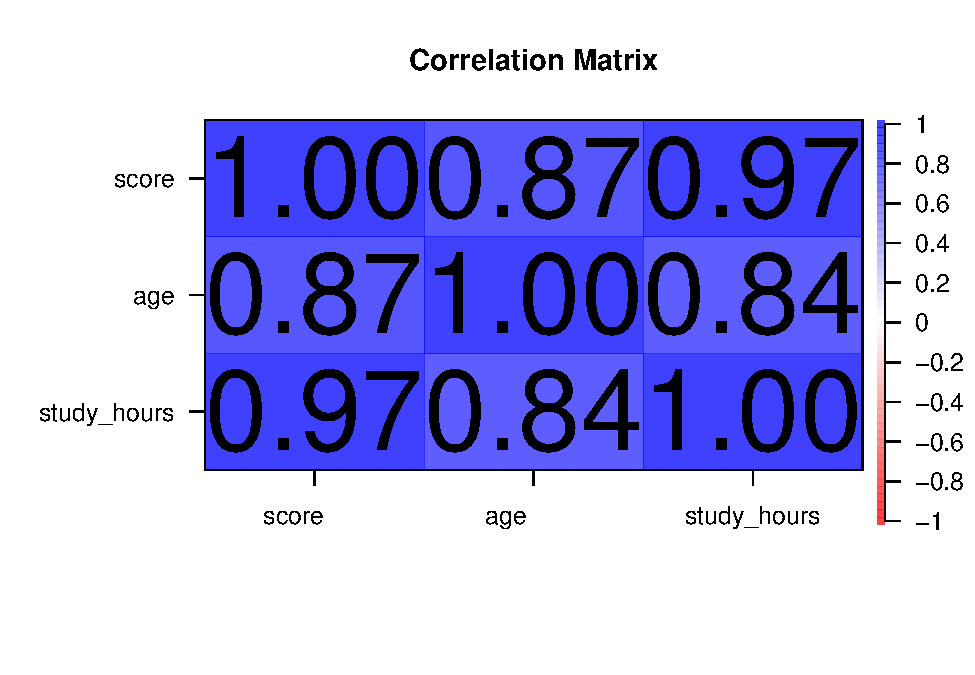
\includegraphics{psych-stats-book_files/figure-latex/unnamed-chunk-39-1.pdf}

\hypertarget{reading-the-corplot-output}{%
\subsubsection{\texorpdfstring{Reading the \texttt{corPlot()} Output}{Reading the corPlot() Output}}\label{reading-the-corplot-output}}

The \texttt{corPlot()} function generates a visual representation of the correlation matrix for a dataset. Here's how to interpret the different elements of the output:

\begin{enumerate}
\def\labelenumi{\arabic{enumi}.}
\item
  \textbf{Correlation Coefficients}: The numerical values in the matrix represent the correlation coefficients between pairs of variables. These coefficients quantify the strength and direction of the linear relationship between variables.

  \begin{itemize}
  \item
    \textbf{Correlation Coefficient (r)}: The value ranges from -1 to 1.

    \begin{itemize}
    \item
      \textbf{r = 1}: Perfect positive correlation.
    \item
      \textbf{r = -1}: Perfect negative correlation.
    \item
      \textbf{r = 0}: No correlation.
    \end{itemize}
  \end{itemize}
\item
  \textbf{Color Coding}: The cells in the matrix are color-coded to reflect the strength and direction of the correlations.

  \begin{itemize}
  \item
    \textbf{Positive Correlations}: Shades of blue indicate positive correlations, with darker shades representing stronger correlations.
  \item
    \textbf{Negative Correlations}: Shades of red indicate negative correlations, with darker shades representing stronger negative correlations.
  \end{itemize}
\item
  \textbf{Significance Levels}: If the \texttt{numbers} argument is set to \texttt{TRUE}, the plot displays the correlation coefficients as numbers within the cells, helping you to identify the exact strength of each correlation.
\end{enumerate}

\textbf{Example Output Interpretation}:

\begin{itemize}
\item
  \textbf{Diagonal Elements}: The diagonal elements of the matrix represent the correlation of each variable with itself, which is always 1.
\item
  \textbf{Off-Diagonal Elements}: The off-diagonal elements show the correlation coefficients between pairs of variables. For instance, a cell showing a value of 0.75 between \texttt{study\_hours} and \texttt{score} indicates a strong positive correlation.
\item
  \textbf{Color Coding}: If a cell is dark blue, it signifies a strong positive correlation, whereas a dark red cell signifies a strong negative correlation. Light colors indicate weaker correlations.
\item
  \textbf{Numerical Values}: The numbers within the cells provide the exact correlation coefficients, making it easy to identify and interpret the strength of the relationships.
\item
  \textbf{Correlation between \texttt{score} and \texttt{study\_hours}}: The correlation coefficient might be 0.75, displayed in a dark blue cell, indicating a strong positive correlation.
\item
  \textbf{Correlation between \texttt{score} and \texttt{age}}: The correlation coefficient might be 0.30, displayed in a light blue cell, indicating a moderate positive correlation.
\item
  \textbf{Correlation between \texttt{age} and \texttt{study\_hours}}: The correlation coefficient might be -0.15, displayed in a light red cell, indicating a weak negative correlation.
\end{itemize}

These interpretations help you understand how the variables in your dataset relate to one another, guiding further analysis and decision-making.

\begin{Shaded}
\begin{Highlighting}[]
\FunctionTok{pairs.panels}\NormalTok{(multi\_var\_data, }
             \AttributeTok{method =} \StringTok{"pearson"}\NormalTok{,  }\CommentTok{\# correlation method}
             \AttributeTok{hist.col =} \StringTok{"blue"}\NormalTok{,    }\CommentTok{\# histogram color}
             \AttributeTok{density =} \ConstantTok{TRUE}\NormalTok{,       }\CommentTok{\# add density plots}
             \AttributeTok{ellipses =} \ConstantTok{TRUE}       \CommentTok{\# add correlation ellipses}
\NormalTok{)}
\end{Highlighting}
\end{Shaded}

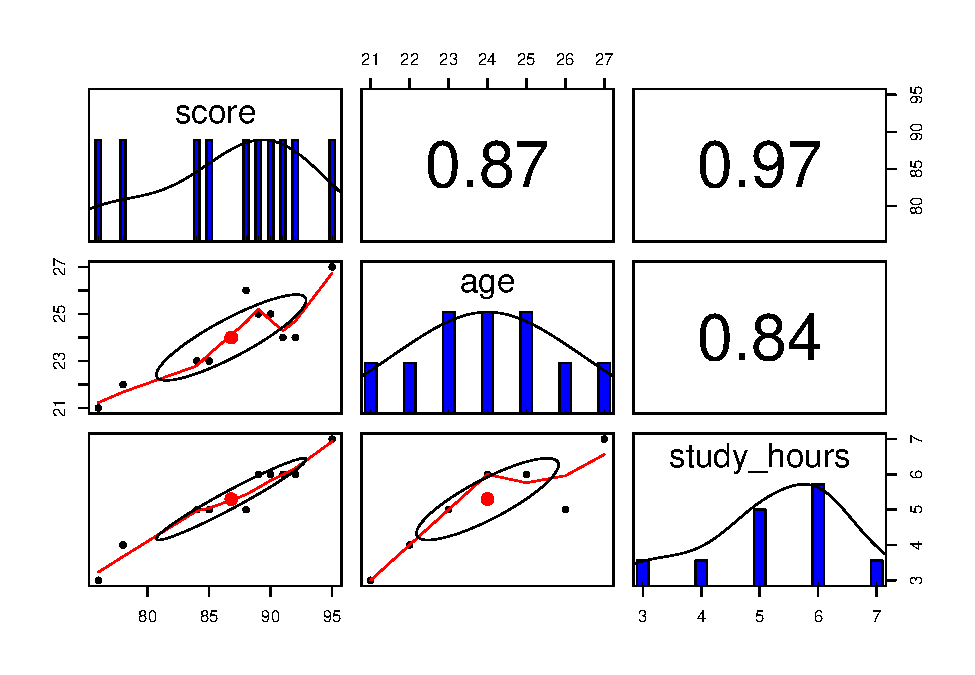
\includegraphics{psych-stats-book_files/figure-latex/Create pair panels-1.pdf}

The \texttt{corPlot()} function displays a correlation matrix with correlation coefficients, while \texttt{pairs.panels()} creates a scatterplot matrix with histograms and density plots, providing a detailed visual summary of the relationships between variables.

\hypertarget{reading-the-pairs.panels-output}{%
\subsubsection{\texorpdfstring{Reading the \texttt{pairs.panels()} Output}{Reading the pairs.panels() Output}}\label{reading-the-pairs.panels-output}}

The \texttt{pairs.panels()} function generates a comprehensive visual summary of the relationships between multiple variables in a dataset. Here's how to interpret the different elements of the output:

\begin{enumerate}
\def\labelenumi{\arabic{enumi}.}
\item
  \textbf{Scatterplots (Lower Triangle)}: The lower triangle of the matrix contains scatterplots for each pair of variables. Each scatterplot shows the relationship between two variables, allowing you to visually assess the strength and direction of their correlation.

  \begin{itemize}
  \item
    \textbf{Positive Correlation}: If the points in the scatterplot form an upward sloping pattern, it indicates a positive correlation between the variables.
  \item
    \textbf{Negative Correlation}: If the points form a downward sloping pattern, it indicates a negative correlation.
  \item
    \textbf{No Correlation}: If the points are widely scattered with no discernible pattern, it suggests little to no correlation.
  \end{itemize}
\item
  \textbf{Histograms (Diagonal)}: The diagonal of the matrix contains histograms for each variable. These histograms show the distribution of values for each variable, helping you to understand their central tendency, variability, and skewness.

  \begin{itemize}
  \item
    \textbf{Symmetric Distribution}: A bell-shaped histogram suggests a normal distribution.
  \item
    \textbf{Skewed Distribution}: A histogram with a long tail on one side indicates skewness in the data.
  \end{itemize}
\item
  \textbf{Correlation Coefficients (Upper Triangle)}: The upper triangle of the matrix contains correlation coefficients for each pair of variables. These coefficients quantify the strength and direction of the linear relationship between variables.

  \begin{itemize}
  \item
    \textbf{Correlation Coefficient (r)}: The value ranges from -1 to 1.

    \begin{itemize}
    \item
      \textbf{r = 1}: Perfect positive correlation.
    \item
      \textbf{r = -1}: Perfect negative correlation.
    \item
      \textbf{r = 0}: No correlation.
    \end{itemize}
  \item
    \textbf{Significance Levels}: The size and color of the coefficients may indicate the significance level, helping you to identify which correlations are statistically significant.
  \end{itemize}
\item
  \textbf{Density Plots (Lower Triangle, if \texttt{density\ =\ TRUE})}: If the \texttt{density} argument is set to \texttt{TRUE}, density plots will be overlaid on the scatterplots. These plots show the density of data points, providing additional insight into the distribution of values.
\item
  \textbf{Correlation Ellipses (Lower Triangle, if \texttt{ellipses\ =\ TRUE})}: If the \texttt{ellipses} argument is set to \texttt{TRUE}, ellipses will be drawn on the scatterplots. These ellipses represent confidence intervals for the correlation, helping you to visually assess the strength and direction of the relationship.
\end{enumerate}

\begin{itemize}
\item
  \textbf{Scatterplots}: You might see an upward slope between \texttt{study\_hours} and \texttt{score}, indicating a positive correlation where increased study hours are associated with higher scores.
\item
  \textbf{Histograms}: The histogram for \texttt{age} might show a relatively uniform distribution, while the histogram for \texttt{study\_hours} could indicate most participants study between 4 to 6 hours.
\item
  \textbf{Correlation Coefficients}: The coefficient between \texttt{score} and \texttt{study\_hours} might be 0.75, suggesting a strong positive correlation. The coefficient between \texttt{age} and \texttt{score} might be lower, indicating a weaker relationship.
\item
  \textbf{Density Plots}: Overlaid on the scatterplots, these provide additional information about the concentration of data points.
\item
  \textbf{Correlation Ellipses}: Ellipses around the scatterplots indicate the confidence intervals, with tighter ellipses suggesting stronger correlations.
\end{itemize}

\hypertarget{conclusion-17}{%
\subsection{Conclusion}\label{conclusion-17}}

The \texttt{psych} package in R offers a comprehensive set of tools for describing and visualizing data, making it invaluable for psychological research. By using functions like \texttt{describe()} for descriptive statistics and \texttt{pairs.panels()} for graphical representations, researchers can gain deeper insights into their data. In the next section, we will explore techniques for importing data from various sources and preparing it for analysis.

\hypertarget{chapter-summary-4}{%
\section{Chapter Summary}\label{chapter-summary-4}}

This chapter provided a comprehensive guide on the essential tasks involved in data computation and manipulation, focusing on the techniques and tools necessary for psychological research. We explored importing data, cleaning data using the \texttt{dplyr} package, and describing data using the \texttt{psych} package, each accompanied by detailed explanations and practical examples.

\hypertarget{key-points-recap-2}{%
\subsection{Key Points Recap}\label{key-points-recap-2}}

\begin{enumerate}
\def\labelenumi{\arabic{enumi}.}
\item
  \textbf{Importance of Data Computation and Manipulation}:

  \begin{itemize}
  \item
    Data computation and manipulation are critical steps in ensuring that data is accurate, consistent, and ready for analysis.
  \item
    These processes allow researchers to clean, organize, and analyze data effectively, leading to more reliable and meaningful conclusions.
  \end{itemize}
\item
  \textbf{Importing Data from Excel Files}:

  \begin{itemize}
  \item
    We covered how to import data from both CSV (.csv) and Excel Workbook (.xlsx) files.
  \item
    Using \texttt{read.csv()} for CSV files and the \texttt{readxl} package for Excel files, we demonstrated practical examples to ensure seamless data importation.
  \end{itemize}
\item
  \textbf{Cleaning Data with \texttt{dplyr}}:

  \begin{itemize}
  \item
    The \texttt{dplyr} package provides powerful and intuitive functions for data manipulation tasks.
  \item
    Key functions include \texttt{filter()}, \texttt{select()}, \texttt{rename()}, \texttt{mutate()}, \texttt{arrange()}, \texttt{summarize()}, and \texttt{group\_by()}.
  \item
    We also covered removing outliers using a custom function and releveling categorical factors for meaningful analysis.
  \item
    Practical examples illustrated how to apply these functions to clean and prepare data for analysis.
  \end{itemize}
\item
  \textbf{Describing Data Using the \texttt{psych} Package}:

  \begin{itemize}
  \item
    The \texttt{psych} package offers tools for generating descriptive statistics and creating graphical summaries.
  \item
    Using the \texttt{describe()} function, we generated comprehensive summaries of datasets.
  \item
    The \texttt{pairs.panels()} function was used to create scatterplot matrices with histograms and correlation coefficients, providing detailed visual summaries of data relationships.
  \item
    The \texttt{corPlot()} function was used to visualize correlation matrices, with detailed explanations on how to interpret the output.
  \end{itemize}
\end{enumerate}

\hypertarget{practical-applications-1}{%
\subsection{Practical Applications}\label{practical-applications-1}}

Throughout the chapter, practical examples demonstrated how to:

\begin{itemize}
\item
  Import data from various file formats.
\item
  Clean and prepare data using \texttt{dplyr}, including handling missing values, renaming variables, removing outliers, and releveling factors.
\item
  Generate descriptive statistics and visualize data using the \texttt{psych} package, including scatterplot matrices and correlation plots.
\end{itemize}

\hypertarget{conclusion-18}{%
\subsection{Conclusion}\label{conclusion-18}}

This chapter highlighted the importance of data computation and manipulation in psychological research. By mastering these techniques and tools, researchers can ensure that their data is well-prepared and accurately analyzed, leading to more robust and credible research outcomes. The knowledge and skills acquired in this chapter lay the foundation for more advanced data analysis techniques covered in subsequent chapters.

\hypertarget{practice-exercises-3}{%
\section{Practice Exercises}\label{practice-exercises-3}}

These exercises aim to test your understanding of data importation, cleaning, and descriptive analysis using the \texttt{dplyr} and \texttt{psych} packages in R. You will apply these concepts to practical problems, ensuring you can efficiently manipulate and describe data.

\hypertarget{exercise-1-importing-data}{%
\subsection{Exercise 1: Importing Data}\label{exercise-1-importing-data}}

\begin{itemize}
\item
  \textbf{Task}: Import data from a CSV file and an Excel file.
\item
  \textbf{Instructions}:

  \begin{enumerate}
  \def\labelenumi{\arabic{enumi}.}
  \item
    Create a CSV file named \texttt{survey\_data.csv} with the following columns: \texttt{id}, \texttt{age}, \texttt{gender}, \texttt{score}.
  \item
    Create an Excel file named \texttt{experiment\_data.xlsx} with the following columns: \texttt{subject\_id}, \texttt{condition}, \texttt{response\_time}.
  \item
    Import both files into R.
  \end{enumerate}
\end{itemize}

\hypertarget{exercise-2-cleaning-data-with-dplyr}{%
\subsection{\texorpdfstring{Exercise 2: Cleaning Data with \texttt{dplyr}}{Exercise 2: Cleaning Data with dplyr}}\label{exercise-2-cleaning-data-with-dplyr}}

\begin{itemize}
\item
  \textbf{Task}: Clean a dataset using various \texttt{dplyr} functions.
\item
  \textbf{Instructions}:

  \begin{enumerate}
  \def\labelenumi{\arabic{enumi}.}
  \tightlist
  \item
    Use the following dataset for the exercise:
  \end{enumerate}
\end{itemize}

\begin{Shaded}
\begin{Highlighting}[]
\NormalTok{data }\OtherTok{\textless{}{-}} \FunctionTok{data.frame}\NormalTok{(}
  \AttributeTok{id =} \DecValTok{1}\SpecialCharTok{:}\DecValTok{10}\NormalTok{,}
  \AttributeTok{age =} \FunctionTok{c}\NormalTok{(}\DecValTok{23}\NormalTok{, }\DecValTok{35}\NormalTok{, }\DecValTok{42}\NormalTok{, }\ConstantTok{NA}\NormalTok{, }\DecValTok{30}\NormalTok{, }\DecValTok{34}\NormalTok{, }\DecValTok{21}\NormalTok{, }\DecValTok{40}\NormalTok{, }\DecValTok{29}\NormalTok{, }\DecValTok{31}\NormalTok{),}
  \AttributeTok{gender =} \FunctionTok{c}\NormalTok{(}\StringTok{"M"}\NormalTok{, }\StringTok{"F"}\NormalTok{, }\StringTok{"F"}\NormalTok{, }\StringTok{"M"}\NormalTok{, }\StringTok{"M"}\NormalTok{, }\StringTok{"F"}\NormalTok{, }\StringTok{"M"}\NormalTok{, }\StringTok{"F"}\NormalTok{, }\StringTok{"M"}\NormalTok{, }\StringTok{"F"}\NormalTok{),}
  \AttributeTok{score =} \FunctionTok{c}\NormalTok{(}\DecValTok{80}\NormalTok{, }\DecValTok{85}\NormalTok{, }\DecValTok{78}\NormalTok{, }\DecValTok{90}\NormalTok{, }\DecValTok{85}\NormalTok{, }\DecValTok{75}\NormalTok{, }\DecValTok{88}\NormalTok{, }\DecValTok{92}\NormalTok{, }\DecValTok{84}\NormalTok{, }\ConstantTok{NA}\NormalTok{)}
\NormalTok{)}
\end{Highlighting}
\end{Shaded}

\begin{verbatim}
2.  Clean the dataset by performing the following steps:

    -   Remove rows with missing values.

    -   Rename the `age` column to `participant_age`.

    -   Create a new column `age_group` based on `participant_age` (Above 30 or 30 and Below).

    -   Remove outliers from the `score` column.

    -   Relevel the `age_group` column to set "30 and Below" as the reference level.
\end{verbatim}

\hypertarget{exercise-3-generating-descriptive-statistics-with-psych}{%
\subsection{\texorpdfstring{Exercise 3: Generating Descriptive Statistics with \texttt{psych}}{Exercise 3: Generating Descriptive Statistics with psych}}\label{exercise-3-generating-descriptive-statistics-with-psych}}

\begin{itemize}
\item
  \textbf{Task}: Generate descriptive statistics for a dataset.
\item
  \textbf{Instructions}:

  \begin{enumerate}
  \def\labelenumi{\arabic{enumi}.}
  \tightlist
  \item
    Use the following dataset for the exercise:
  \end{enumerate}
\end{itemize}

\begin{Shaded}
\begin{Highlighting}[]
\NormalTok{test\_scores }\OtherTok{\textless{}{-}} \FunctionTok{data.frame}\NormalTok{(}
  \AttributeTok{id =} \DecValTok{1}\SpecialCharTok{:}\DecValTok{10}\NormalTok{,}
  \AttributeTok{score =} \FunctionTok{c}\NormalTok{(}\DecValTok{85}\NormalTok{, }\DecValTok{90}\NormalTok{, }\DecValTok{78}\NormalTok{, }\DecValTok{92}\NormalTok{, }\DecValTok{88}\NormalTok{, }\DecValTok{76}\NormalTok{, }\DecValTok{95}\NormalTok{, }\DecValTok{89}\NormalTok{, }\DecValTok{84}\NormalTok{, }\DecValTok{91}\NormalTok{)}
\NormalTok{)}
\end{Highlighting}
\end{Shaded}

\begin{verbatim}
2.  Generate descriptive statistics using the `describe()` function from the `psych` package.
\end{verbatim}

\hypertarget{exercise-4-visualizing-data-with-psych}{%
\subsection{\texorpdfstring{Exercise 4: Visualizing Data with \texttt{psych}}{Exercise 4: Visualizing Data with psych}}\label{exercise-4-visualizing-data-with-psych}}

\begin{itemize}
\item
  \textbf{Task}: Create graphical summaries of a dataset using the \texttt{psych} package.
\item
  \textbf{Instructions}:

  \begin{enumerate}
  \def\labelenumi{\arabic{enumi}.}
  \tightlist
  \item
    Use the following dataset for the exercise:
  \end{enumerate}
\end{itemize}

\begin{Shaded}
\begin{Highlighting}[]
\NormalTok{multi\_var\_data }\OtherTok{\textless{}{-}} \FunctionTok{data.frame}\NormalTok{(}
  \AttributeTok{score =} \FunctionTok{c}\NormalTok{(}\DecValTok{85}\NormalTok{, }\DecValTok{90}\NormalTok{, }\DecValTok{78}\NormalTok{, }\DecValTok{92}\NormalTok{, }\DecValTok{88}\NormalTok{, }\DecValTok{76}\NormalTok{, }\DecValTok{95}\NormalTok{, }\DecValTok{89}\NormalTok{, }\DecValTok{84}\NormalTok{, }\DecValTok{91}\NormalTok{),}
  \AttributeTok{age =} \FunctionTok{c}\NormalTok{(}\DecValTok{23}\NormalTok{, }\DecValTok{25}\NormalTok{, }\DecValTok{22}\NormalTok{, }\DecValTok{24}\NormalTok{, }\DecValTok{26}\NormalTok{, }\DecValTok{21}\NormalTok{, }\DecValTok{27}\NormalTok{, }\DecValTok{25}\NormalTok{, }\DecValTok{23}\NormalTok{, }\DecValTok{24}\NormalTok{),}
  \AttributeTok{study\_hours =} \FunctionTok{c}\NormalTok{(}\DecValTok{5}\NormalTok{, }\DecValTok{6}\NormalTok{, }\DecValTok{4}\NormalTok{, }\DecValTok{6}\NormalTok{, }\DecValTok{5}\NormalTok{, }\DecValTok{3}\NormalTok{, }\DecValTok{7}\NormalTok{, }\DecValTok{6}\NormalTok{, }\DecValTok{5}\NormalTok{, }\DecValTok{6}\NormalTok{)}
\NormalTok{)}
\end{Highlighting}
\end{Shaded}

\begin{verbatim}
2.  Create a correlation plot using the `corPlot()` function.

3.  Create pair panels using the `pairs.panels()` function.
\end{verbatim}

\hypertarget{linear-and-non-linear-transformations-of-data}{%
\chapter{Linear and Non-Linear Transformations of Data}\label{linear-and-non-linear-transformations-of-data}}

\hypertarget{chapter-overview}{%
\section{Chapter Overview}\label{chapter-overview}}

In the realm of psychological research and data analysis, transforming data is a crucial step to ensure accurate and meaningful interpretations. Chapter 6 delves into the concepts of linear and non-linear transformations of data, focusing on two primary techniques: mean-centering and Z-scores. These transformations play a vital role in preparing data for statistical analysis, making it easier to interpret results and draw valid conclusions.

This chapter is designed to provide a comprehensive understanding of these transformations, enriched with practical examples, real-world applications, and hands-on exercises using R. By the end of this chapter, you will be able to:

\begin{enumerate}
\def\labelenumi{\arabic{enumi}.}
\item
  \textbf{Understand the Importance of Data Transformation}: Learn why transforming data is essential in statistical analysis and how it can impact your results.
\item
  \textbf{Perform Mean-Centering}: Understand the concept of mean-centering, its mathematical formulation, and its application in psychological research. You will learn how to perform mean-centering in R and visualize its effects on data.
\item
  \textbf{Calculate Z-Scores}: Grasp the concept of Z-scores, their importance in standardizing data, and their role in comparing different datasets. You will learn to compute Z-scores in R and interpret their meaning.
\item
  \textbf{Combine Transformations}: Explore how mean-centering and Z-scores can be used together to enhance data analysis. Practical examples will illustrate the benefits of combining these transformations.
\item
  \textbf{Apply Non-Linear Transformations}: Discover various types of non-linear transformations, such as logarithmic, square root, and inverse transformations. Understand when and why to use these transformations and how to implement them in R.
\item
  \textbf{Interpret Real-World Examples}: Through practical examples and real-world applications, you will see how these transformations are used in psychological research and other fields.
\item
  \textbf{Hands-On Practice}: Engage in exercises designed to reinforce your understanding of the concepts covered. These exercises will provide an opportunity to apply transformations to real datasets and interpret the results.
\end{enumerate}

\hypertarget{key-topics-covered}{%
\subsubsection{Key Topics Covered}\label{key-topics-covered}}

\begin{itemize}
\item
  \textbf{Mean-Centering}

  \begin{itemize}
  \item
    Definition and importance
  \item
    Mathematical formula
  \item
    Practical examples
  \item
    Real-world applications
  \item
    R code implementation
  \end{itemize}
\item
  \textbf{Z-Scores}

  \begin{itemize}
  \item
    Definition and importance
  \item
    Mathematical formula
  \item
    Practical examples
  \item
    Real-world applications
  \item
    R code implementation
  \end{itemize}
\item
  \textbf{Combining Transformations}

  \begin{itemize}
  \item
    Mean-centering and Z-scores together
  \item
    Practical example
  \item
    R code implementation
  \end{itemize}
\item
  \textbf{Non-Linear Transformations}

  \begin{itemize}
  \item
    Introduction to non-linear transformations
  \item
    Types of non-linear transformations
  \item
    Practical examples
  \item
    Real-world applications
  \item
    R code implementation
  \end{itemize}
\end{itemize}

By transforming data effectively, researchers can uncover patterns and relationships that might be obscured in the raw data, leading to more robust and reliable conclusions. This chapter will equip you with the knowledge and skills necessary to perform these transformations and apply them in your research projects.

\hypertarget{mean-centering}{%
\section{Mean-Centering}\label{mean-centering}}

\hypertarget{definition-and-importance-1}{%
\subsection{Definition and Importance}\label{definition-and-importance-1}}

Mean-centering is a simple but powerful technique used to adjust data by subtracting the average (mean) of the dataset from each individual data point. This transformation helps to focus on the differences between data points rather than their absolute values, making it easier to compare and interpret the data.

\textbf{Why is Mean-Centering Important?}

\begin{enumerate}
\def\labelenumi{\arabic{enumi}.}
\tightlist
\item
  \textbf{Understanding Data Differences}:

  \begin{itemize}
  \tightlist
  \item
    When you mean-center data, you're essentially asking, ``How does each individual data point compare to the average?'' This is useful in many types of analysis because it helps you see patterns and relationships more clearly.
  \end{itemize}
\item
  \textbf{Preparing Data for Further Analysis}:

  \begin{itemize}
  \tightlist
  \item
    Mean-centering is often a first step before conducting more complex analyses, as it simplifies the data and makes it easier to work with. For example, if you were comparing test scores between two groups, mean-centering those scores would help you see how each group performs relative to the average.
  \end{itemize}
\end{enumerate}

\hypertarget{mathematical-formula}{%
\subsection{Mathematical Formula}\label{mathematical-formula}}

The mathematical formula for mean-centering is straightforward. For each data point \(X_i\) in a dataset, the mean-centered value \(X_{\text{centered}, i}\) is calculated by subtracting the mean \(\bar{X}\) of the dataset from the original value:

\[
X_{\text{centered}} = X - \bar{X}
\]

Where: - \(X\) is the original value. - \(\bar{X}\) is the mean of the dataset. - \(X_{\text{centered}}\) is the mean-centered value.

\hypertarget{practical-examples}{%
\subsection{Practical Examples}\label{practical-examples}}

\textbf{Example 1: Mean-Centering a Dataset of Students' Test Scores}

Imagine you have a list of students' test scores, and you want to see how each student's score compares to the average score. Here's how you can do that with mean-centering:

\textbf{Dataset}: - Scores: 85, 90, 78, 92, 88, 76, 95, 89, 84, 91

First, calculate the average (mean) score:

\[
\bar{X} = \frac{85 + 90 + 78 + 92 + 88 + 76 + 95 + 89 + 84 + 91}{10} = 86.8
\]

Next, subtract this mean from each student's score to get the mean-centered values. This will show how each score compares to the average.

\textbf{Example 2: Mean-Centering a Dataset of Reaction Times in a Cognitive Experiment}

Suppose you're conducting a cognitive experiment where you measure how quickly participants respond to a stimulus. You have the following reaction times (in milliseconds):

\textbf{Dataset}: - Reaction Times: 250, 340, 295, 310, 275, 325, 290, 360, 285, 310

To mean-center these reaction times, start by calculating the average reaction time:

\[
\bar{X} = \frac{250 + 340 + 295 + 310 + 275 + 325 + 290 + 360 + 285 + 310}{10} = 304
\]

Then, subtract this average from each reaction time to see how quickly or slowly each participant responded compared to the average.

\hypertarget{real-world-applications}{%
\subsection{Real-World Applications}\label{real-world-applications}}

\begin{enumerate}
\def\labelenumi{\arabic{enumi}.}
\tightlist
\item
  \textbf{Comparing Groups with Different Starting Points}:

  \begin{itemize}
  \tightlist
  \item
    Mean-centering is often used in research to make comparisons between groups easier. For instance, if you were comparing stress levels in two different groups of people, and one group started with higher stress levels than the other, mean-centering their stress scores would help you see how much each group's stress changed relative to their own starting point.
  \end{itemize}
\item
  \textbf{Simplifying Data Interpretation}:

  \begin{itemize}
  \tightlist
  \item
    When you have data from multiple sources or categories, mean-centering helps you focus on the relative differences within those categories rather than being distracted by the overall level of the data. This makes it easier to understand and interpret the results.
  \end{itemize}
\end{enumerate}

\hypertarget{r-code-implementation}{%
\subsection{R Code Implementation}\label{r-code-implementation}}

\textbf{Demonstrating Mean-Centering with R Code}

Let's use R to mean-center the dataset of students' test scores.

\begin{Shaded}
\begin{Highlighting}[]
\CommentTok{\# Sample data: Students\textquotesingle{} test scores}
\NormalTok{scores }\OtherTok{\textless{}{-}} \FunctionTok{c}\NormalTok{(}\DecValTok{85}\NormalTok{, }\DecValTok{90}\NormalTok{, }\DecValTok{78}\NormalTok{, }\DecValTok{92}\NormalTok{, }\DecValTok{88}\NormalTok{, }\DecValTok{76}\NormalTok{, }\DecValTok{95}\NormalTok{, }\DecValTok{89}\NormalTok{, }\DecValTok{84}\NormalTok{, }\DecValTok{91}\NormalTok{)}

\CommentTok{\# Calculate the mean of the scores}
\NormalTok{mean\_scores }\OtherTok{\textless{}{-}} \FunctionTok{mean}\NormalTok{(scores)}

\CommentTok{\# Mean{-}centering the scores}
\NormalTok{mean\_centered\_scores }\OtherTok{\textless{}{-}}\NormalTok{ scores }\SpecialCharTok{{-}}\NormalTok{ mean\_scores}

\CommentTok{\# Display the mean{-}centered scores}
\NormalTok{mean\_centered\_scores}
\end{Highlighting}
\end{Shaded}

\begin{verbatim}
##  [1]  -1.8   3.2  -8.8   5.2   1.2 -10.8   8.2   2.2  -2.8   4.2
\end{verbatim}

\textbf{Output}: The output will show the mean-centered values, which indicate how each student's score compares to the average score. A positive value means the score is above average, while a negative value means it's below average.

\textbf{Plotting the Original and Mean-Centered Data}

To better visualize the effect of mean-centering, you can plot both the original and mean-centered scores.

\begin{Shaded}
\begin{Highlighting}[]
\CommentTok{\# Display the mean{-}centered scores}
\NormalTok{mean\_centered\_scores}
\end{Highlighting}
\end{Shaded}

\begin{verbatim}
##  [1]  -1.8   3.2  -8.8   5.2   1.2 -10.8   8.2   2.2  -2.8   4.2
\end{verbatim}

\begin{Shaded}
\begin{Highlighting}[]
\CommentTok{\# Determine y{-}axis limits to accommodate both original and mean{-}centered data}
\NormalTok{y\_limits }\OtherTok{\textless{}{-}} \FunctionTok{range}\NormalTok{(}\FunctionTok{c}\NormalTok{(scores, mean\_centered\_scores))}

\CommentTok{\# Plotting original and mean{-}centered data}
\FunctionTok{plot}\NormalTok{(scores, }\AttributeTok{type =} \StringTok{"b"}\NormalTok{, }\AttributeTok{col =} \StringTok{"blue"}\NormalTok{, }\AttributeTok{ylab =} \StringTok{"Scores"}\NormalTok{, }\AttributeTok{xlab =} \StringTok{"Index"}\NormalTok{, }\AttributeTok{main =} \StringTok{"Original vs Mean{-}Centered Scores"}\NormalTok{, }\AttributeTok{ylim =}\NormalTok{ y\_limits)}
\FunctionTok{lines}\NormalTok{(mean\_centered\_scores, }\AttributeTok{type =} \StringTok{"b"}\NormalTok{, }\AttributeTok{col =} \StringTok{"red"}\NormalTok{)}
\FunctionTok{legend}\NormalTok{(}\StringTok{"topright"}\NormalTok{, }\AttributeTok{legend =} \FunctionTok{c}\NormalTok{(}\StringTok{"Original"}\NormalTok{, }\StringTok{"Mean{-}Centered"}\NormalTok{), }\AttributeTok{col =} \FunctionTok{c}\NormalTok{(}\StringTok{"blue"}\NormalTok{, }\StringTok{"red"}\NormalTok{), }\AttributeTok{lty =} \DecValTok{1}\NormalTok{)}
\end{Highlighting}
\end{Shaded}

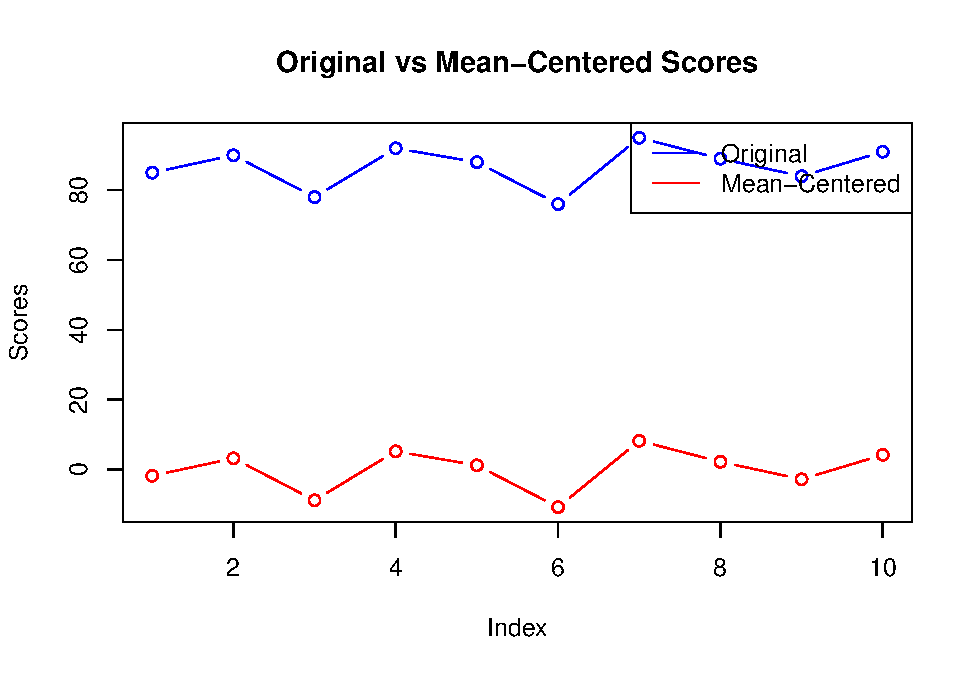
\includegraphics{psych-stats-book_files/figure-latex/unnamed-chunk-44-1.pdf}

In this plot, the blue line represents the original scores, while the red line represents the mean-centered scores. Notice how the mean-centered scores are centered around zero, making it easy to see how each student's performance compares to the average.

This section has introduced the concept of mean-centering, explained its importance, and demonstrated its application using practical examples and R code. By mean-centering your data, you can more easily compare and interpret individual data points relative to the group as a whole. This is a valuable tool in data analysis, helping to reveal patterns and relationships that might otherwise be hidden.

\hypertarget{z-scores}{%
\section{Z-Scores}\label{z-scores}}

\hypertarget{definition-and-importance-2}{%
\subsection{Definition and Importance}\label{definition-and-importance-2}}

Z-scores are a statistical measure that describe a value's position relative to the mean of a group of values, measured in terms of standard deviations from the mean. In simpler terms, a Z-score tells you how ``unusual'' or ``typical'' a value is compared to the rest of the data.

\textbf{Why Are Z-Scores Important?}

\begin{enumerate}
\def\labelenumi{\arabic{enumi}.}
\tightlist
\item
  \textbf{Standardizing Data for Fair Comparison}:

  \begin{itemize}
  \tightlist
  \item
    Z-scores allow you to compare different datasets or different groups within a dataset, even if they have different means or variations. By converting data to Z-scores, you're essentially putting everything on the same scale.
  \end{itemize}
\item
  \textbf{Understanding Relative Position}:

  \begin{itemize}
  \tightlist
  \item
    Z-scores help you see whether a value is above or below the average, and by how much. This is useful when you want to understand how an individual score compares to the group as a whole.
  \end{itemize}
\end{enumerate}

\hypertarget{mathematical-formula-1}{%
\subsection{Mathematical Formula}\label{mathematical-formula-1}}

The formula for calculating a Z-score is:

\[
Z = \frac{X - \bar{X}}{\sigma}
\]

Where: - \(X\) is the original value. - \(\bar{X}\) is the mean of the dataset. - \(\sigma\) is the standard deviation of the dataset. - \(Z\) is the Z-score, which tells you how many standard deviations the value \(X\) is from the mean.

\hypertarget{practical-examples-1}{%
\subsection{Practical Examples}\label{practical-examples-1}}

\textbf{Example 1: Calculating Z-Scores for a Dataset of Exam Scores}

Imagine you have a list of exam scores and want to know how each student's score compares to the average. Z-scores can help you do this by showing how much each score differs from the average.

\textbf{Dataset}: - Scores: 85, 90, 78, 92, 88, 76, 95, 89, 84, 91

First, calculate the mean (\(\bar{X}\)) and standard deviation (\(\sigma\)) of the scores:

\[
\bar{X} = \frac{85 + 90 + 78 + 92 + 88 + 76 + 95 + 89 + 84 + 91}{10} = 86.8
\]

\[
\sigma = \sqrt{\frac{(85-86.8)^2 + (90-86.8)^2 + \dots + (91-86.8)^2}{10}} = 5.67
\]

Next, calculate the Z-score for each score to see how far each one is from the average:

\[
Z = \frac{85 - 86.8}{5.67} = -0.32
\]

\textbf{Example 2: Using Z-Scores to Compare Heights of Individuals from Different Age Groups}

Let's say you have height data for people in different age groups. By converting their heights to Z-scores, you can compare how tall someone is relative to others in their age group.

\textbf{Dataset}: - Heights: 160, 170, 165, 175, 168, 172, 169, 166, 171, 167

For each age group, you calculate the mean and standard deviation, then convert the heights to Z-scores to see how each individual compares to their peers.

\hypertarget{real-world-applications-1}{%
\subsection{Real-World Applications}\label{real-world-applications-1}}

\begin{enumerate}
\def\labelenumi{\arabic{enumi}.}
\tightlist
\item
  \textbf{Identifying Outliers}:

  \begin{itemize}
  \tightlist
  \item
    Z-scores are often used to spot outliers in a dataset. If a Z-score is very high or very low (typically beyond ±2 or ±3), it indicates that the value is much higher or lower than the average and might be considered an outlier.
  \end{itemize}
\item
  \textbf{Comparing Scores in Psychological Assessments}:

  \begin{itemize}
  \tightlist
  \item
    In psychological testing, Z-scores can be used to compare an individual's score to a standard or normative sample. For example, Z-scores can show how a person's test results compare to the average results of a larger population.
  \end{itemize}
\end{enumerate}

\hypertarget{r-code-implementation-1}{%
\subsection{R Code Implementation}\label{r-code-implementation-1}}

\textbf{Demonstrating Calculation of Z-Scores with R Code}

Let's calculate the Z-scores for our exam scores dataset.

\begin{Shaded}
\begin{Highlighting}[]
\CommentTok{\# Sample data: Exam scores}
\NormalTok{scores }\OtherTok{\textless{}{-}} \FunctionTok{c}\NormalTok{(}\DecValTok{85}\NormalTok{, }\DecValTok{90}\NormalTok{, }\DecValTok{78}\NormalTok{, }\DecValTok{92}\NormalTok{, }\DecValTok{88}\NormalTok{, }\DecValTok{76}\NormalTok{, }\DecValTok{95}\NormalTok{, }\DecValTok{89}\NormalTok{, }\DecValTok{84}\NormalTok{, }\DecValTok{91}\NormalTok{)}

\CommentTok{\# Calculate the mean of the scores}
\NormalTok{mean\_scores }\OtherTok{\textless{}{-}} \FunctionTok{mean}\NormalTok{(scores)}

\CommentTok{\# Calculate the standard deviation of the scores}
\NormalTok{sd\_scores }\OtherTok{\textless{}{-}} \FunctionTok{sd}\NormalTok{(scores)}

\CommentTok{\# Calculate the Z{-}scores}
\NormalTok{z\_scores }\OtherTok{\textless{}{-}}\NormalTok{ (scores }\SpecialCharTok{{-}}\NormalTok{ mean\_scores) }\SpecialCharTok{/}\NormalTok{ sd\_scores}

\CommentTok{\# Display the Z{-}scores}
\NormalTok{z\_scores}
\end{Highlighting}
\end{Shaded}

\begin{verbatim}
##  [1] -0.2956519  0.5256035 -1.4454095  0.8541056  0.1971013 -1.7739117
##  [7]  1.3468589  0.3613524 -0.4599030  0.6898545
\end{verbatim}

\textbf{Output}: The output will show the Z-scores for each student's exam score. A Z-score above 0 means the score is above average, while a Z-score below 0 means it is below average.

\textbf{Visualizing Z-Scores Using a Standard Normal Distribution}

To better understand how these Z-scores are distributed, we can plot them on a histogram.

\begin{Shaded}
\begin{Highlighting}[]
\CommentTok{\# Plotting Z{-}scores}
\FunctionTok{hist}\NormalTok{(z\_scores, }\AttributeTok{breaks =} \DecValTok{10}\NormalTok{, }\AttributeTok{col =} \StringTok{"blue"}\NormalTok{, }\AttributeTok{xlab =} \StringTok{"Z{-}Scores"}\NormalTok{, }\AttributeTok{main =} \StringTok{"Histogram of Z{-}Scores"}\NormalTok{)}
\FunctionTok{abline}\NormalTok{(}\AttributeTok{v =} \DecValTok{0}\NormalTok{, }\AttributeTok{col =} \StringTok{"red"}\NormalTok{, }\AttributeTok{lwd =} \DecValTok{2}\NormalTok{)}
\end{Highlighting}
\end{Shaded}

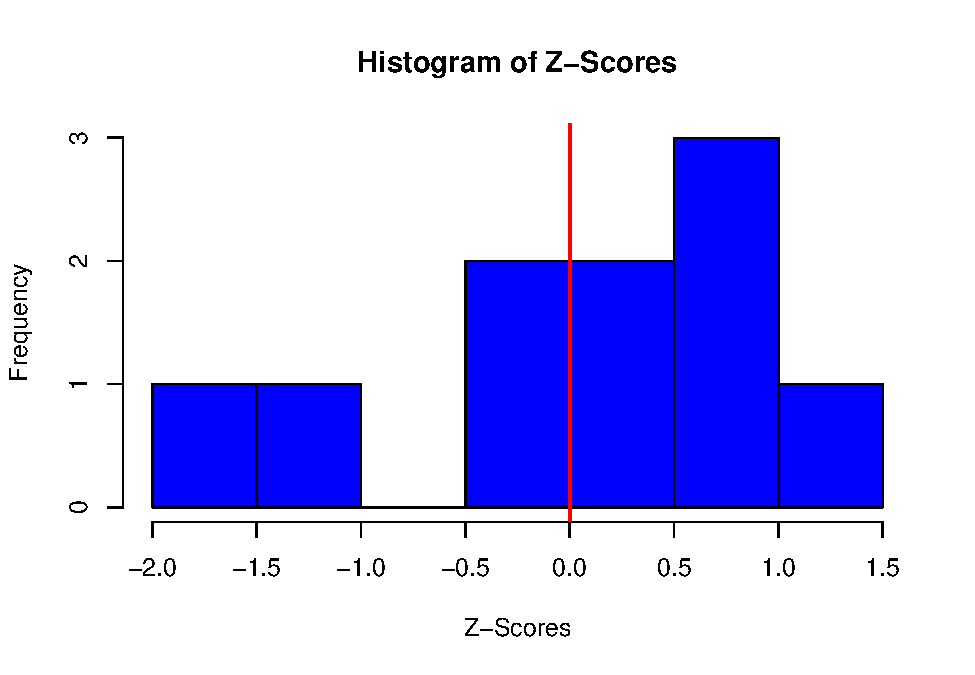
\includegraphics{psych-stats-book_files/figure-latex/unnamed-chunk-46-1.pdf}

In this plot:

\begin{itemize}
\item
  The histogram shows the spread of Z-scores.
\item
  The red vertical line at \(Z = 0\) represents the mean. Scores to the right of this line are above average, and those to the left are below
\end{itemize}

This section has provided a simplified explanation of Z-scores, their purpose, and practical examples of how they are calculated and used. Z-scores are a valuable tool for standardizing data, making it easier to compare values across different datasets, and for identifying outliers in your data.

\hypertarget{combining-transformations}{%
\section{Combining Transformations}\label{combining-transformations}}

\hypertarget{mean-centering-and-z-scores-together}{%
\subsection{Mean-Centering and Z-Scores Together}\label{mean-centering-and-z-scores-together}}

Sometimes, when analyzing data, you might want to apply both mean-centering and Z-scores to the same dataset. Each transformation has its own purpose, and when used together, they can give you a deeper understanding of your data.

\textbf{Why Use Both Mean-Centering and Z-Scores?}

\begin{enumerate}
\def\labelenumi{\arabic{enumi}.}
\tightlist
\item
  \textbf{Mean-Centering}:

  \begin{itemize}
  \tightlist
  \item
    Mean-centering is useful for adjusting your data so that the mean of the dataset is zero. This makes it easier to understand how each data point compares to the average.
  \end{itemize}
\item
  \textbf{Z-Scores}:

  \begin{itemize}
  \tightlist
  \item
    Z-scores go a step further by not only centering the data around zero but also scaling it based on the standard deviation. This standardization allows you to see how far each data point is from the mean in terms of standard deviations, making it easier to compare values across different datasets or groups.
  \end{itemize}
\end{enumerate}

\textbf{When to Combine Them?} - You might combine these transformations when you want to center your data (subtract the mean) and also standardize it (divide by the standard deviation). This is particularly useful when you need to compare data points from different groups or when you're preparing data for certain statistical analyses.

\hypertarget{practical-example-1}{%
\subsection{Practical Example}\label{practical-example-1}}

\textbf{Example: Combining Mean-Centering and Z-Scores in a Dataset of Reaction Times}

Let's say you're working with reaction time data from an experiment. You want to know not only how each participant's reaction time compares to the average (mean-centering) but also how it compares in terms of standard deviations from the mean (Z-scores).

\textbf{Dataset}: - Reaction Times (in milliseconds): 250, 340, 295, 310, 275, 325, 290, 360, 285, 310

First, you'll mean-center the data to see how each reaction time compares to the average reaction time. Then, you'll calculate the Z-scores to understand how each reaction time compares to the overall distribution of times in terms of standard deviations.

\hypertarget{r-code-implementation-2}{%
\subsection{R Code Implementation}\label{r-code-implementation-2}}

Let's walk through how to perform both transformations using R.

\begin{Shaded}
\begin{Highlighting}[]
\CommentTok{\# Sample data: Reaction times in milliseconds}
\NormalTok{reaction\_times }\OtherTok{\textless{}{-}} \FunctionTok{c}\NormalTok{(}\DecValTok{250}\NormalTok{, }\DecValTok{340}\NormalTok{, }\DecValTok{295}\NormalTok{, }\DecValTok{310}\NormalTok{, }\DecValTok{275}\NormalTok{, }\DecValTok{325}\NormalTok{, }\DecValTok{290}\NormalTok{, }\DecValTok{360}\NormalTok{, }\DecValTok{285}\NormalTok{, }\DecValTok{310}\NormalTok{)}

\CommentTok{\# Step 1: Calculate the mean of the reaction times}
\NormalTok{mean\_reaction\_time }\OtherTok{\textless{}{-}} \FunctionTok{mean}\NormalTok{(reaction\_times)}

\CommentTok{\# Step 2: Mean{-}center the reaction times}
\NormalTok{mean\_centered\_times }\OtherTok{\textless{}{-}}\NormalTok{ reaction\_times }\SpecialCharTok{{-}}\NormalTok{ mean\_reaction\_time}

\CommentTok{\# Step 3: Calculate the standard deviation of the original reaction times}
\NormalTok{sd\_reaction\_time }\OtherTok{\textless{}{-}} \FunctionTok{sd}\NormalTok{(reaction\_times)}

\CommentTok{\# Step 4: Calculate Z{-}scores for the mean{-}centered reaction times}
\NormalTok{z\_scores\_centered }\OtherTok{\textless{}{-}}\NormalTok{ mean\_centered\_times }\SpecialCharTok{/}\NormalTok{ sd\_reaction\_time}

\CommentTok{\# Display the mean{-}centered reaction times}
\NormalTok{mean\_centered\_times}
\end{Highlighting}
\end{Shaded}

\begin{verbatim}
##  [1] -54  36  -9   6 -29  21 -14  56 -19   6
\end{verbatim}

\begin{Shaded}
\begin{Highlighting}[]
\CommentTok{\# Display the Z{-}scores for the mean{-}centered reaction times}
\NormalTok{z\_scores\_centered}
\end{Highlighting}
\end{Shaded}

\begin{verbatim}
##  [1] -1.6762608  1.1175072 -0.2793768  0.1862512 -0.9002141  0.6518792
##  [7] -0.4345861  1.7383445 -0.5897954  0.1862512
\end{verbatim}

\textbf{Output}:

\begin{itemize}
\item
  The \texttt{mean\_centered\_times} will show how each reaction time differs from the average reaction time.
\item
  The \texttt{z\_scores\_centered} will show how many standard deviations each mean-centered reaction time is from the mean.
\end{itemize}

\textbf{Visualizing the Transformations}

To better understand the effects of these transformations, let's plot the original reaction times, the mean-centered reaction times, and the Z-scores.

\begin{Shaded}
\begin{Highlighting}[]
\CommentTok{\# Plotting original, mean{-}centered, and Z{-}scores}
\FunctionTok{par}\NormalTok{(}\AttributeTok{mfrow =} \FunctionTok{c}\NormalTok{(}\DecValTok{3}\NormalTok{, }\DecValTok{1}\NormalTok{))  }\CommentTok{\# Set up the plotting area to have 3 plots, one above the other}

\CommentTok{\# Plot original reaction times}
\FunctionTok{plot}\NormalTok{(reaction\_times, }\AttributeTok{type =} \StringTok{"b"}\NormalTok{, }\AttributeTok{col =} \StringTok{"blue"}\NormalTok{, }\AttributeTok{ylab =} \StringTok{"Reaction Times"}\NormalTok{, }\AttributeTok{xlab =} \StringTok{"Index"}\NormalTok{, }\AttributeTok{main =} \StringTok{"Original Reaction Times"}\NormalTok{)}

\CommentTok{\# Plot mean{-}centered reaction times}
\FunctionTok{plot}\NormalTok{(mean\_centered\_times, }\AttributeTok{type =} \StringTok{"b"}\NormalTok{, }\AttributeTok{col =} \StringTok{"green"}\NormalTok{, }\AttributeTok{ylab =} \StringTok{"Mean{-}Centered"}\NormalTok{, }\AttributeTok{xlab =} \StringTok{"Index"}\NormalTok{, }\AttributeTok{main =} \StringTok{"Mean{-}Centered Reaction Times"}\NormalTok{)}

\CommentTok{\# Plot Z{-}scores of mean{-}centered reaction times}
\FunctionTok{plot}\NormalTok{(z\_scores\_centered, }\AttributeTok{type =} \StringTok{"b"}\NormalTok{, }\AttributeTok{col =} \StringTok{"red"}\NormalTok{, }\AttributeTok{ylab =} \StringTok{"Z{-}Scores"}\NormalTok{, }\AttributeTok{xlab =} \StringTok{"Index"}\NormalTok{, }\AttributeTok{main =} \StringTok{"Z{-}Scores of Mean{-}Centered Reaction Times"}\NormalTok{)}
\end{Highlighting}
\end{Shaded}

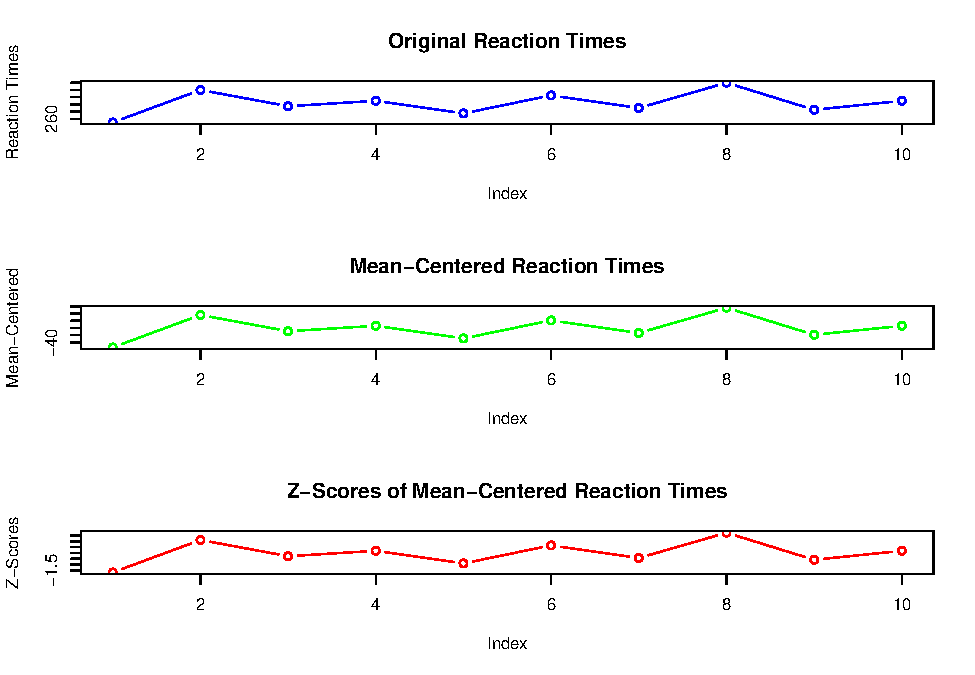
\includegraphics{psych-stats-book_files/figure-latex/unnamed-chunk-48-1.pdf}

\textbf{Explanation of the Plots}:

\begin{enumerate}
\def\labelenumi{\arabic{enumi}.}
\item
  \textbf{Original Reaction Times (Blue)}:

  \begin{itemize}
  \tightlist
  \item
    This plot shows the raw reaction times as they were originally measured.
  \end{itemize}
\item
  \textbf{Mean-Centered Reaction Times (Green)}:

  \begin{itemize}
  \tightlist
  \item
    This plot shows the reaction times after subtracting the average reaction time. The data is now centered around zero, making it easier to see how each time compares to the average.
  \end{itemize}
\item
  \textbf{Z-Scores of Mean-Centered Reaction Times (Red)}:

  \begin{itemize}
  \tightlist
  \item
    This plot shows the reaction times after both mean-centering and standardizing them. The Z-scores tell you how far each mean-centered time is from the average in terms of standard deviations, making it easier to identify outliers or unusual reaction times.
  \end{itemize}
\end{enumerate}

\hypertarget{summary}{%
\subsection{Summary}\label{summary}}

By combining mean-centering and Z-scores, you gain a more nuanced understanding of your data. Mean-centering adjusts the data so that the average is zero, highlighting deviations from the mean. Z-scores take this a step further by scaling these deviations in terms of standard deviations, allowing for easier comparison across different datasets or groups. This combined approach is particularly useful in psychological research and data analysis, where understanding relative differences and standardizing data are key to drawing accurate conclusions.

\hypertarget{non-linear-transformations}{%
\section{Non-Linear Transformations}\label{non-linear-transformations}}

\hypertarget{introduction-to-non-linear-transformations}{%
\subsection{Introduction to Non-Linear Transformations}\label{introduction-to-non-linear-transformations}}

In data analysis, not all data behaves in a simple, straightforward way. Sometimes, the relationship between variables is not linear, meaning that the data doesn't follow a straight line when graphed. In such cases, non-linear transformations can be helpful. These transformations change the scale or distribution of the data in a way that makes it easier to analyze and interpret.

\textbf{When and Why Are Non-Linear Transformations Used?}

\begin{enumerate}
\def\labelenumi{\arabic{enumi}.}
\tightlist
\item
  \textbf{Handling Skewed Data}:

  \begin{itemize}
  \tightlist
  \item
    Sometimes, data can be skewed, meaning that it is not evenly distributed. For example, if most people in a dataset earn a low income, but a few people earn very high incomes, the data will be right-skewed. Non-linear transformations, like the logarithmic transformation, can help to ``pull in'' extreme values and make the distribution more balanced.
  \end{itemize}
\item
  \textbf{Stabilizing Variance}:

  \begin{itemize}
  \tightlist
  \item
    In some datasets, the variability (or spread) of the data might change depending on the value of the variable. For instance, reaction times might have more variability for slower responses than for faster ones. A square root transformation can stabilize this variance, making the data easier to analyze.
  \end{itemize}
\item
  \textbf{Meeting Assumptions of Statistical Tests}:

  \begin{itemize}
  \tightlist
  \item
    Many statistical tests assume that the data follows a normal distribution (a bell-shaped curve). Non-linear transformations can help make the data conform more closely to these assumptions, which makes the results of statistical tests more reliable.
  \end{itemize}
\end{enumerate}

\hypertarget{types-of-non-linear-transformations}{%
\subsection{Types of Non-Linear Transformations}\label{types-of-non-linear-transformations}}

There are several common types of non-linear transformations, each useful in different situations:

\begin{enumerate}
\def\labelenumi{\arabic{enumi}.}
\tightlist
\item
  \textbf{Logarithmic Transformation}

  \begin{itemize}
  \item
    The logarithmic transformation (often simply called a ``log transformation'') is used to reduce the impact of extreme values in a dataset. It is particularly useful for right-skewed data, where a few very large values dominate the dataset.
  \item
    \textbf{Formula}: \[
    Y_{\text{log}} = \log(X)
    \]
  \item
    \textbf{Example}: If you have income data where most people earn between \$30,000 and \$50,000 but a few people earn millions, applying a log transformation can make the distribution of incomes more normal.
  \end{itemize}
\item
  \textbf{Square Root Transformation}

  \begin{itemize}
  \item
    The square root transformation is often used to stabilize variance. It's useful when the data has a wider spread at higher values.
  \item
    \textbf{Formula}:
  \end{itemize}
\end{enumerate}

\[
Y_{\text{sqrt}} = \sqrt{X}
\]

\begin{itemize}
\tightlist
\item
  \textbf{Example}: If you have reaction time data where the variability increases with longer times, applying a square root transformation can reduce this variability, making the data more consistent.
\end{itemize}

\begin{enumerate}
\def\labelenumi{\arabic{enumi}.}
\setcounter{enumi}{2}
\tightlist
\item
  \textbf{Inverse Transformation}

  \begin{itemize}
  \item
    The inverse transformation is used to ``flip'' the data and reduce the impact of large values. This transformation is useful when high values in the dataset need to be ``compressed.''
  \item
    \textbf{Formula}:
  \end{itemize}
\end{enumerate}

\[
Y_{\text{inv}} = \frac{1}{X}
\]

\begin{itemize}
\tightlist
\item
  \textbf{Example}: Inverting the data can help with situations where large values need to be brought closer to smaller values, such as with response times in tasks where quicker responses are more common.
\end{itemize}

\hypertarget{practical-examples-2}{%
\subsection{Practical Examples}\label{practical-examples-2}}

\textbf{Example 1: Logarithmic Transformation of Income Data to Reduce Skewness}

Let's consider a dataset of annual incomes where most people earn between \$30,000 and \$50,000, but a few earn much more, even up to \$1,000,000. This type of data is likely to be right-skewed. Applying a logarithmic transformation can help ``pull in'' the higher incomes and make the distribution more balanced.

\textbf{Example 2: Square Root Transformation of Reaction Time Data to Stabilize Variance}

Imagine you're analyzing reaction times in an experiment, and you notice that the variability of response times is larger for slower responses. By applying a square root transformation, you can stabilize the variance, making the data easier to interpret and analyze.

\hypertarget{real-world-applications-2}{%
\subsection{Real-World Applications}\label{real-world-applications-2}}

\begin{enumerate}
\def\labelenumi{\arabic{enumi}.}
\item
  \textbf{Use in Psychological Research}:

  \begin{itemize}
  \tightlist
  \item
    In psychological studies, non-linear transformations are often used to meet the assumptions of statistical tests. For example, when analyzing response times or survey data, researchers might use square root or log transformations to normalize the data.
  \end{itemize}
\item
  \textbf{Application in Economic Data}:

  \begin{itemize}
  \tightlist
  \item
    Economic data, such as income or wealth distributions, are often heavily skewed. Logarithmic transformations are commonly used in economics to handle these skewed distributions, making the data more suitable for analysis and interpretation.
  \end{itemize}
\end{enumerate}

\hypertarget{r-code-implementation-3}{%
\subsection{R Code Implementation}\label{r-code-implementation-3}}

Let's walk through how to apply these non-linear transformations using R.

\begin{Shaded}
\begin{Highlighting}[]
\CommentTok{\# Sample data: Income data in thousands of dollars}
\NormalTok{income }\OtherTok{\textless{}{-}} \FunctionTok{c}\NormalTok{(}\DecValTok{30}\NormalTok{, }\DecValTok{45}\NormalTok{, }\DecValTok{70}\NormalTok{, }\DecValTok{120}\NormalTok{, }\DecValTok{25}\NormalTok{, }\DecValTok{60}\NormalTok{, }\DecValTok{100}\NormalTok{, }\DecValTok{85}\NormalTok{, }\DecValTok{40}\NormalTok{, }\DecValTok{300}\NormalTok{)}

\CommentTok{\# Logarithmic Transformation}
\NormalTok{log\_income }\OtherTok{\textless{}{-}} \FunctionTok{log}\NormalTok{(income)}

\CommentTok{\# Square Root Transformation}
\NormalTok{sqrt\_income }\OtherTok{\textless{}{-}} \FunctionTok{sqrt}\NormalTok{(income)}

\CommentTok{\# Inverse Transformation}
\NormalTok{inv\_income }\OtherTok{\textless{}{-}} \DecValTok{1} \SpecialCharTok{/}\NormalTok{ income}

\CommentTok{\# Display the transformed data}
\NormalTok{log\_income}
\end{Highlighting}
\end{Shaded}

\begin{verbatim}
##  [1] 3.401197 3.806662 4.248495 4.787492 3.218876 4.094345 4.605170 4.442651
##  [9] 3.688879 5.703782
\end{verbatim}

\begin{Shaded}
\begin{Highlighting}[]
\NormalTok{sqrt\_income}
\end{Highlighting}
\end{Shaded}

\begin{verbatim}
##  [1]  5.477226  6.708204  8.366600 10.954451  5.000000  7.745967 10.000000
##  [8]  9.219544  6.324555 17.320508
\end{verbatim}

\begin{Shaded}
\begin{Highlighting}[]
\NormalTok{inv\_income}
\end{Highlighting}
\end{Shaded}

\begin{verbatim}
##  [1] 0.033333333 0.022222222 0.014285714 0.008333333 0.040000000 0.016666667
##  [7] 0.010000000 0.011764706 0.025000000 0.003333333
\end{verbatim}

\textbf{Output}:

\begin{itemize}
\item
  \texttt{log\_income}: This will show the income data after applying a logarithmic transformation. The larger values will be ``pulled in,'' reducing the skewness of the data.
\item
  \texttt{sqrt\_income}: This will show the income data after applying a square root transformation. This transformation helps stabilize variance in the data.
\item
  \texttt{inv\_income}: This will show the income data after applying an inverse transformation. The largest values will be compressed more than the smaller ones.
\end{itemize}

\textbf{Visualizing the Transformations}

To see how these transformations affect the data, let's plot the original and transformed datasets.

\begin{Shaded}
\begin{Highlighting}[]
\CommentTok{\# Set up the plotting area to have 2x2 plots}
\FunctionTok{par}\NormalTok{(}\AttributeTok{mfrow =} \FunctionTok{c}\NormalTok{(}\DecValTok{2}\NormalTok{, }\DecValTok{2}\NormalTok{))}

\CommentTok{\# Plot original income data}
\FunctionTok{hist}\NormalTok{(income, }\AttributeTok{breaks =} \DecValTok{10}\NormalTok{, }\AttributeTok{col =} \StringTok{"blue"}\NormalTok{, }\AttributeTok{xlab =} \StringTok{"Income"}\NormalTok{, }\AttributeTok{main =} \StringTok{"Original Income"}\NormalTok{)}

\CommentTok{\# Plot log{-}transformed income data}
\FunctionTok{hist}\NormalTok{(log\_income, }\AttributeTok{breaks =} \DecValTok{10}\NormalTok{, }\AttributeTok{col =} \StringTok{"green"}\NormalTok{, }\AttributeTok{xlab =} \StringTok{"Log(Income)"}\NormalTok{, }\AttributeTok{main =} \StringTok{"Log Transformed Income"}\NormalTok{)}

\CommentTok{\# Plot square root{-}transformed income data}
\FunctionTok{hist}\NormalTok{(sqrt\_income, }\AttributeTok{breaks =} \DecValTok{10}\NormalTok{, }\AttributeTok{col =} \StringTok{"orange"}\NormalTok{, }\AttributeTok{xlab =} \StringTok{"Sqrt(Income)"}\NormalTok{, }\AttributeTok{main =} \StringTok{"Square Root Transformed Income"}\NormalTok{)}

\CommentTok{\# Plot inverse{-}transformed income data}
\FunctionTok{hist}\NormalTok{(inv\_income, }\AttributeTok{breaks =} \DecValTok{10}\NormalTok{, }\AttributeTok{col =} \StringTok{"red"}\NormalTok{, }\AttributeTok{xlab =} \StringTok{"1/Income"}\NormalTok{, }\AttributeTok{main =} \StringTok{"Inverse Transformed Income"}\NormalTok{)}
\end{Highlighting}
\end{Shaded}

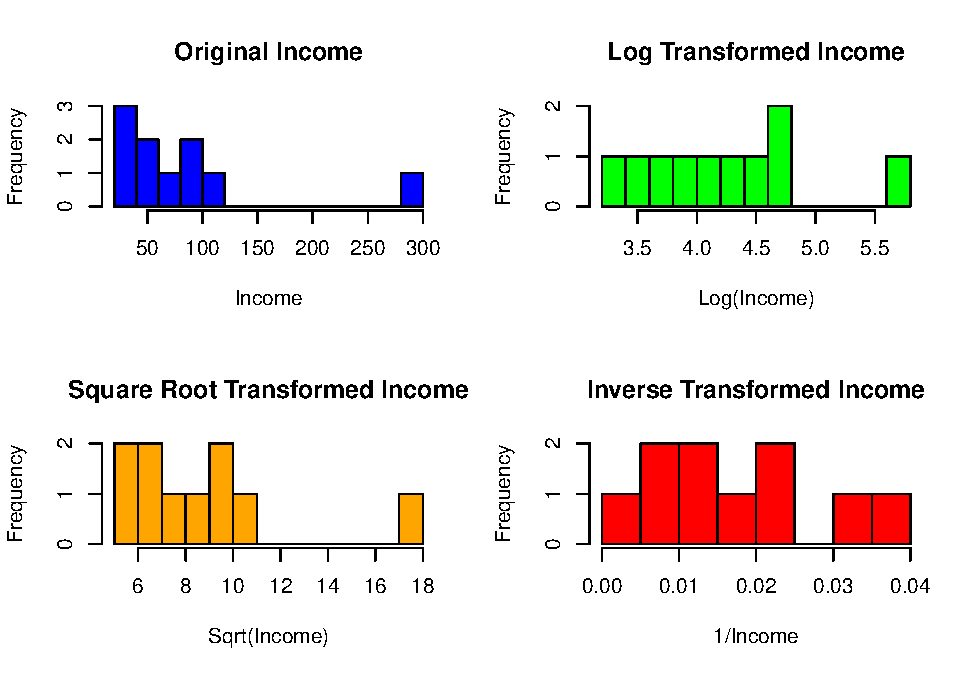
\includegraphics{psych-stats-book_files/figure-latex/unnamed-chunk-50-1.pdf}

\textbf{Explanation of the Plots}:

\begin{enumerate}
\def\labelenumi{\arabic{enumi}.}
\item
  \textbf{Original Income Data (Blue)}:

  \begin{itemize}
  \tightlist
  \item
    This plot shows the original distribution of income data, which might be skewed if there are a few very large values.
  \end{itemize}
\item
  \textbf{Log-Transformed Income Data (Green)}:

  \begin{itemize}
  \tightlist
  \item
    The log transformation reduces the impact of the large incomes, resulting in a more balanced distribution.
  \end{itemize}
\item
  \textbf{Square Root-Transformed Income Data (Orange)}:

  \begin{itemize}
  \tightlist
  \item
    The square root transformation helps stabilize the variance, making the spread of the data more consistent across different income levels.
  \end{itemize}
\item
  \textbf{Inverse-Transformed Income Data (Red)}:

  \begin{itemize}
  \tightlist
  \item
    The inverse transformation compresses the larger values, flipping and bringing them closer to the smaller values.
  \end{itemize}
\end{enumerate}

\hypertarget{summary-1}{%
\subsection{Summary}\label{summary-1}}

Non-linear transformations are powerful tools that allow you to handle skewed data, stabilize variance, and meet the assumptions of statistical tests. By applying transformations like logarithmic, square root, or inverse, you can make your data more suitable for analysis and easier to interpret. These techniques are commonly used in psychological research, economics, and other fields where data may not always follow a straightforward, linear pattern.

\hypertarget{chapter-summary-5}{%
\section{Chapter Summary}\label{chapter-summary-5}}

In this chapter, we explored various data transformation techniques, focusing on both linear and non-linear transformations. These transformations are essential tools in data analysis, helping to prepare and modify data to meet the assumptions of statistical tests, reduce skewness, stabilize variance, and make data more interpretable.

\textbf{Key Takeaways:}

\begin{enumerate}
\def\labelenumi{\arabic{enumi}.}
\tightlist
\item
  \textbf{Mean-Centering}:

  \begin{itemize}
  \tightlist
  \item
    \textbf{Definition}: Mean-centering involves subtracting the mean of the dataset from each data point, effectively centering the data around zero.
  \item
    \textbf{Importance}: It simplifies the interpretation of data by focusing on how each value compares to the average, and it is often used as a preparatory step in data analysis.
  \item
    \textbf{Application}: Mean-centering is particularly useful when comparing groups or preparing data for more complex analyses.
  \end{itemize}
\item
  \textbf{Z-Scores}:

  \begin{itemize}
  \tightlist
  \item
    \textbf{Definition}: A Z-score standardizes data by measuring how far a value is from the mean, in terms of standard deviations.
  \item
    \textbf{Importance}: Z-scores allow for direct comparison between different datasets or groups, even if they have different means or variances. They also help identify outliers.
  \item
    \textbf{Application}: Z-scores are widely used in psychological assessments and in any analysis where comparing standardized values is important.
  \end{itemize}
\item
  \textbf{Combining Transformations}:

  \begin{itemize}
  \tightlist
  \item
    \textbf{Purpose}: Combining mean-centering and Z-scores provides a more nuanced understanding of data, particularly when both centering and scaling are needed.
  \item
    \textbf{Application}: This combination is useful in various analytical contexts, especially when preparing data for regression analysis or other statistical tests.
  \end{itemize}
\item
  \textbf{Non-Linear Transformations}:

  \begin{itemize}
  \tightlist
  \item
    \textbf{Logarithmic Transformation}: Reduces skewness by pulling in extreme values, making data more normally distributed.
  \item
    \textbf{Square Root Transformation}: Stabilizes variance, especially useful for data where variability increases with the value.
  \item
    \textbf{Inverse Transformation}: Compresses large values, useful when dealing with data that has extreme high values.
  \item
    \textbf{Importance}: Non-linear transformations are crucial when data does not meet the assumptions of linearity or normality, and they are often applied in psychological research, economics, and other fields dealing with skewed or heteroscedastic data.
  \end{itemize}
\end{enumerate}

\textbf{Practical Application}:
Throughout the chapter, we demonstrated how to apply these transformations using R, providing practical examples and R code implementations. These examples showed how transformations can make data more suitable for analysis, ultimately leading to more accurate and meaningful results.

\textbf{Conclusion}:
Data transformations, whether linear or non-linear, are powerful tools that can greatly enhance the clarity and reliability of your data analysis. By understanding when and how to apply these transformations, you can ensure that your data is in the best possible shape for whatever statistical tests or analyses you plan to perform. As you move forward in your studies, remember that mastering these foundational techniques will be invaluable in your research and data analysis endeavors.

\hypertarget{practice-exercises-4}{%
\section{Practice Exercises}\label{practice-exercises-4}}

These exercises are designed to reinforce your understanding of the concepts covered in this chapter, including mean-centering, Z-scores, and non-linear transformations. For each exercise, you will apply these transformations to provided datasets, interpret the results, and understand their implications.

\hypertarget{exercise-1-mean-centering}{%
\subsection{Exercise 1: Mean-Centering}\label{exercise-1-mean-centering}}

\textbf{Dataset}:
- A dataset of monthly expenses (in dollars): \texttt{expenses\ \textless{}-\ c(1200,\ 1500,\ 1100,\ 1800,\ 1300,\ 1700,\ 1250,\ 1400,\ 1600,\ 1350)}

\textbf{Tasks}:\\
1. Calculate the mean of the expenses.\\
2. Mean-center the dataset by subtracting the mean from each value.\\
3. Plot the original and mean-centered expenses on the same graph.\\
4. \textbf{Interpretation}: Describe how the mean-centered values relate to the average expense. What does a positive or negative mean-centered value indicate?

\begin{Shaded}
\begin{Highlighting}[]
\NormalTok{expenses }\OtherTok{\textless{}{-}} \FunctionTok{c}\NormalTok{(}\DecValTok{1200}\NormalTok{, }\DecValTok{1500}\NormalTok{, }\DecValTok{1100}\NormalTok{, }\DecValTok{1800}\NormalTok{, }\DecValTok{1300}\NormalTok{, }\DecValTok{1700}\NormalTok{, }\DecValTok{1250}\NormalTok{, }\DecValTok{1400}\NormalTok{, }\DecValTok{1600}\NormalTok{, }\DecValTok{1350}\NormalTok{)}
\CommentTok{\# Calculate the mean of the expenses}


\CommentTok{\# Mean{-}center the expenses}


\CommentTok{\# Plot the original and mean{-}centered expenses}

\CommentTok{\# Interpretation: Provide your answer here}
\end{Highlighting}
\end{Shaded}

\hypertarget{exercise-2-z-scores}{%
\subsection{Exercise 2: Z-Scores}\label{exercise-2-z-scores}}

\textbf{Dataset}:
- A dataset of test scores: \texttt{test\_scores\ \textless{}-\ c(65,\ 78,\ 82,\ 91,\ 70,\ 88,\ 75,\ 95,\ 80,\ 85)}

\textbf{Tasks}:\\
1. Calculate the mean and standard deviation of the test scores.\\
2. Compute the Z-scores for each test score.\\
3. Create a histogram of the Z-scores and add a vertical line at Z = 0.\\
4. \textbf{Interpretation}: Explain what a Z-score greater than 0 or less than 0 indicates about a test score relative to the average. How would you identify outliers using Z-scores?

\begin{Shaded}
\begin{Highlighting}[]
\NormalTok{test\_scores }\OtherTok{\textless{}{-}} \FunctionTok{c}\NormalTok{(}\DecValTok{65}\NormalTok{, }\DecValTok{78}\NormalTok{, }\DecValTok{82}\NormalTok{, }\DecValTok{91}\NormalTok{, }\DecValTok{70}\NormalTok{, }\DecValTok{88}\NormalTok{, }\DecValTok{75}\NormalTok{, }\DecValTok{95}\NormalTok{, }\DecValTok{80}\NormalTok{, }\DecValTok{85}\NormalTok{)}

\CommentTok{\# Calculate the mean and standard deviation of the test scores}


\CommentTok{\# Compute the Z{-}scores}


\CommentTok{\# Create a histogram of the Z{-}scores}

\CommentTok{\# Interpretation: Provide your answer here}
\end{Highlighting}
\end{Shaded}

\hypertarget{exercise-3-combining-mean-centering-and-z-scores}{%
\subsection{Exercise 3: Combining Mean-Centering and Z-Scores}\label{exercise-3-combining-mean-centering-and-z-scores}}

\textbf{Dataset}:
- A dataset of reaction times (in milliseconds): \texttt{reaction\_times\ \textless{}-\ c(250,\ 340,\ 295,\ 310,\ 275,\ 325,\ 290,\ 360,\ 285,\ 310)}

\textbf{Tasks}:\\
1. Mean-center the reaction times.\\
2. Calculate the Z-scores for the mean-centered reaction times.\\
3. Plot the original reaction times, mean-centered times, and Z-scores on separate graphs.\\
4. \textbf{Interpretation}: Discuss the effect of applying both transformations. How do the Z-scores help you understand the reaction times in comparison to the mean-centered data?

\begin{Shaded}
\begin{Highlighting}[]
\NormalTok{reaction\_times }\OtherTok{\textless{}{-}} \FunctionTok{c}\NormalTok{(}\DecValTok{250}\NormalTok{, }\DecValTok{340}\NormalTok{, }\DecValTok{295}\NormalTok{, }\DecValTok{310}\NormalTok{, }\DecValTok{275}\NormalTok{, }\DecValTok{325}\NormalTok{, }\DecValTok{290}\NormalTok{, }\DecValTok{360}\NormalTok{, }\DecValTok{285}\NormalTok{, }\DecValTok{310}\NormalTok{)}

\CommentTok{\# Mean{-}center the reaction times}


\CommentTok{\# Calculate the Z{-}scores for the mean{-}centered reaction times}


\CommentTok{\# Plot the original reaction times, mean{-}centered times, and Z{-}scores}


\CommentTok{\# Interpretation: Provide your answer here}
\end{Highlighting}
\end{Shaded}

\hypertarget{exercise-4-non-linear-transformations}{%
\subsection{Exercise 4: Non-Linear Transformations}\label{exercise-4-non-linear-transformations}}

\textbf{Dataset}:
- A dataset of annual incomes (in thousands of dollars): \texttt{income\ \textless{}-\ c(30,\ 45,\ 70,\ 120,\ 25,\ 60,\ 100,\ 85,\ 40,\ 300)}

\textbf{Tasks}:\\
1. Apply a logarithmic transformation to the income data.\\
2. Apply a square root transformation to the income data.\\
3. Apply an inverse transformation to the income data.\\
4. Plot histograms of the original and transformed datasets.\\
5. \textbf{Interpretation}: Compare the distributions of the original and transformed data. How does each transformation affect the spread and shape of the data? When might each transformation be most useful?

\begin{Shaded}
\begin{Highlighting}[]
\NormalTok{income }\OtherTok{\textless{}{-}} \FunctionTok{c}\NormalTok{(}\DecValTok{30}\NormalTok{, }\DecValTok{45}\NormalTok{, }\DecValTok{70}\NormalTok{, }\DecValTok{120}\NormalTok{, }\DecValTok{25}\NormalTok{, }\DecValTok{60}\NormalTok{, }\DecValTok{100}\NormalTok{, }\DecValTok{85}\NormalTok{, }\DecValTok{40}\NormalTok{, }\DecValTok{300}\NormalTok{)}

\CommentTok{\# Apply a logarithmic transformation}


\CommentTok{\# Apply a square root transformation}


\CommentTok{\# Apply an inverse transformation}


\CommentTok{\# Plot histograms of the original and transformed data}


\CommentTok{\# Interpretation: Provide your answer here}
\end{Highlighting}
\end{Shaded}

\hypertarget{ggplot2-and-graphing-data-in-apa-formatting}{%
\chapter{ggplot2 and Graphing Data in APA Formatting}\label{ggplot2-and-graphing-data-in-apa-formatting}}

\hypertarget{chapter-overview-introduction-to-data-visualization}{%
\section{Chapter Overview: Introduction to Data Visualization}\label{chapter-overview-introduction-to-data-visualization}}

\hypertarget{importance-of-graphing-in-research}{%
\subsection{Importance of Graphing in Research}\label{importance-of-graphing-in-research}}

Graphing, or data visualization, is a fundamental aspect of psychological research. It serves as a powerful tool to summarize complex datasets and convey findings in a clear, concise, and visually appealing manner. In the realm of psychological science, where researchers often deal with large amounts of data, effective visualization is crucial for several reasons:

\begin{enumerate}
\def\labelenumi{\arabic{enumi}.}
\tightlist
\item
  \textbf{Enhancing Understanding}:

  \begin{itemize}
  \tightlist
  \item
    Graphs help to make sense of data by transforming raw numbers into visual representations, making patterns, trends, and relationships easier to identify and understand. Whether it's tracking changes over time, comparing groups, or highlighting correlations, a well-crafted graph can quickly convey the essence of the data.
  \end{itemize}
\item
  \textbf{Communicating Results}:

  \begin{itemize}
  \tightlist
  \item
    In research, it's not just about discovering new insights; it's also about communicating those findings to others---whether that's peers, policymakers, or the public. Graphs are a universal language that transcends technical jargon, allowing researchers to effectively communicate their results to a broad audience. A clear and accurate graph can often tell a story more compellingly than a table of numbers ever could.
  \end{itemize}
\item
  \textbf{Supporting Evidence}:

  \begin{itemize}
  \tightlist
  \item
    Graphs are often used to support the conclusions drawn from statistical analyses. They provide a visual confirmation of the trends and patterns identified in the data, helping to bolster the credibility of the research. In many cases, journals and conferences require visual representations of data to accompany statistical results, making graphing an essential skill for researchers.
  \end{itemize}
\end{enumerate}

\hypertarget{common-types-of-graphs-in-psychological-research}{%
\subsection{Common Types of Graphs in Psychological Research}\label{common-types-of-graphs-in-psychological-research}}

Psychological research frequently relies on several key types of graphs to present data. Each type serves a different purpose and is selected based on the nature of the data and the research question. Here are the most common types:

\begin{enumerate}
\def\labelenumi{\arabic{enumi}.}
\tightlist
\item
  \textbf{Bar Graphs}:

  \begin{itemize}
  \tightlist
  \item
    \textbf{Purpose}: Bar graphs are used to compare the values of different groups or categories. They are particularly useful when you want to show the differences between discrete categories, such as the mean scores of different groups in an experiment.
  \item
    \textbf{Example}: A bar graph might be used to display the average test scores of students in different teaching methods.
  \end{itemize}
\item
  \textbf{Line Graphs}:

  \begin{itemize}
  \tightlist
  \item
    \textbf{Purpose}: Line graphs are ideal for showing trends over time or the relationship between two continuous variables. They are often used when the data points are related in a sequential order, such as time-series data.
  \item
    \textbf{Example}: A line graph could be used to track changes in anxiety levels over several weeks of a treatment program.
  \end{itemize}
\item
  \textbf{Scatter Plots}:

  \begin{itemize}
  \tightlist
  \item
    \textbf{Purpose}: Scatter plots are used to examine the relationship between two continuous variables. Each point on the graph represents an observation, allowing researchers to see patterns, correlations, or outliers.
  \item
    \textbf{Example}: A scatter plot might be used to explore the relationship between hours studied and exam scores among students.
  \end{itemize}
\item
  \textbf{Histograms}:

  \begin{itemize}
  \tightlist
  \item
    \textbf{Purpose}: Histograms are used to show the distribution of a single continuous variable. They help to visualize the frequency of data points within specified ranges, providing insights into the shape of the data distribution.
  \item
    \textbf{Example}: A histogram could be used to display the distribution of reaction times in a cognitive experiment.
  \end{itemize}
\item
  \textbf{Box Plots}:

  \begin{itemize}
  \tightlist
  \item
    \textbf{Purpose}: Box plots (or box-and-whisker plots) are used to summarize the distribution of a dataset, showing the median, quartiles, and potential outliers. They are particularly useful for comparing distributions across different groups.
  \item
    \textbf{Example}: A box plot might be used to compare the distribution of stress scores across different age groups.
  \end{itemize}
\end{enumerate}

In this chapter, we will explore the basics of creating these types of graphs using the powerful ggplot2 package in R. We will start with the fundamentals, ensuring you have a solid understanding of how to construct and customize these visualizations. Later, we will focus on how to adjust these graphs to adhere to APA formatting guidelines, which is essential for presenting your research in a professional and standardized manner.

\hypertarget{getting-started-with-ggplot2}{%
\section{Getting Started with ggplot2}\label{getting-started-with-ggplot2}}

\hypertarget{what-is-ggplot2}{%
\subsection{What is ggplot2?}\label{what-is-ggplot2}}

\textbf{ggplot2} is a powerful and flexible data visualization package in R that allows you to create a wide variety of graphs, from simple scatter plots to complex multi-layered visualizations. Unlike the base R plotting system, which can be somewhat rigid and limited in its capabilities, ggplot2 offers a much more intuitive and layered approach to creating graphs.

\textbf{Why Use ggplot2?}
- \textbf{Customizability}: ggplot2 allows you to fine-tune every aspect of your graph, from the colors and shapes of points to the labels and themes. This means you can create visualizations that are not only accurate but also aesthetically pleasing and tailored to your specific needs.
- \textbf{Layered Approach}: ggplot2 uses a concept called the ``grammar of graphics,'' which makes it easy to build up a plot in layers. This approach allows you to start with a basic plot and gradually add more complexity, such as colors, labels, or statistical summaries, in a structured way.
- \textbf{Consistency}: The syntax of ggplot2 is consistent across different types of plots. Once you learn the basic structure, you can easily apply it to a wide range of graphs, making the learning curve less steep.
- \textbf{Integration with R}: ggplot2 integrates seamlessly with R's data structures, such as data frames and tibbles, allowing you to directly plot data from your analyses.

\textbf{Comparison with Base R Plotting Functions}
- \textbf{Base R}: In base R, plots are created using functions like \texttt{plot()}, \texttt{hist()}, or \texttt{barplot()}. While these functions are straightforward, they can be limited in terms of customization. For example, adding multiple layers or modifying specific elements (like changing the color of just one bar in a bar plot) can be cumbersome.
- \textbf{ggplot2}: In contrast, ggplot2's layered approach makes it easy to add or modify elements. For instance, you can start with a simple scatter plot and then layer on a regression line, customize the colors, and add labels, all with a few lines of code.

Here's a simple comparison:

\begin{itemize}
\tightlist
\item
  \textbf{Base R Scatter Plot}:
\end{itemize}

\begin{Shaded}
\begin{Highlighting}[]
  \FunctionTok{plot}\NormalTok{(mpg }\SpecialCharTok{\textasciitilde{}}\NormalTok{ wt, }\AttributeTok{data =}\NormalTok{ mtcars)}
\end{Highlighting}
\end{Shaded}

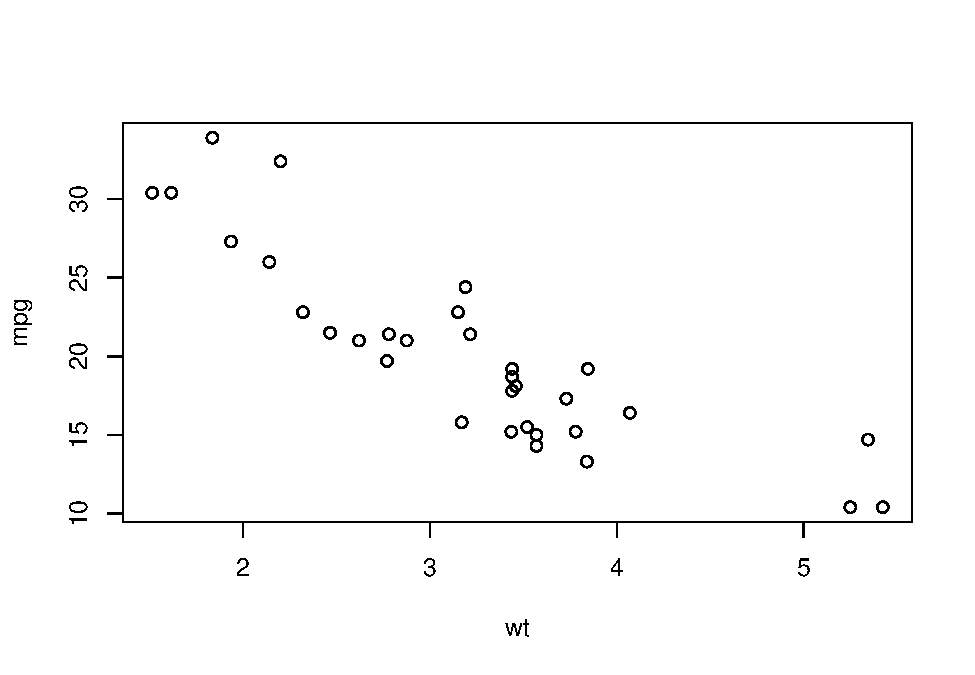
\includegraphics{psych-stats-book_files/figure-latex/unnamed-chunk-55-1.pdf}

\begin{itemize}
\tightlist
\item
  \textbf{ggplot2 Scatter Plot}:
\end{itemize}

\begin{Shaded}
\begin{Highlighting}[]
  \FunctionTok{ggplot}\NormalTok{(mtcars, }\FunctionTok{aes}\NormalTok{(}\AttributeTok{x =}\NormalTok{ wt, }\AttributeTok{y =}\NormalTok{ mpg)) }\SpecialCharTok{+}
    \FunctionTok{geom\_point}\NormalTok{()}
\end{Highlighting}
\end{Shaded}

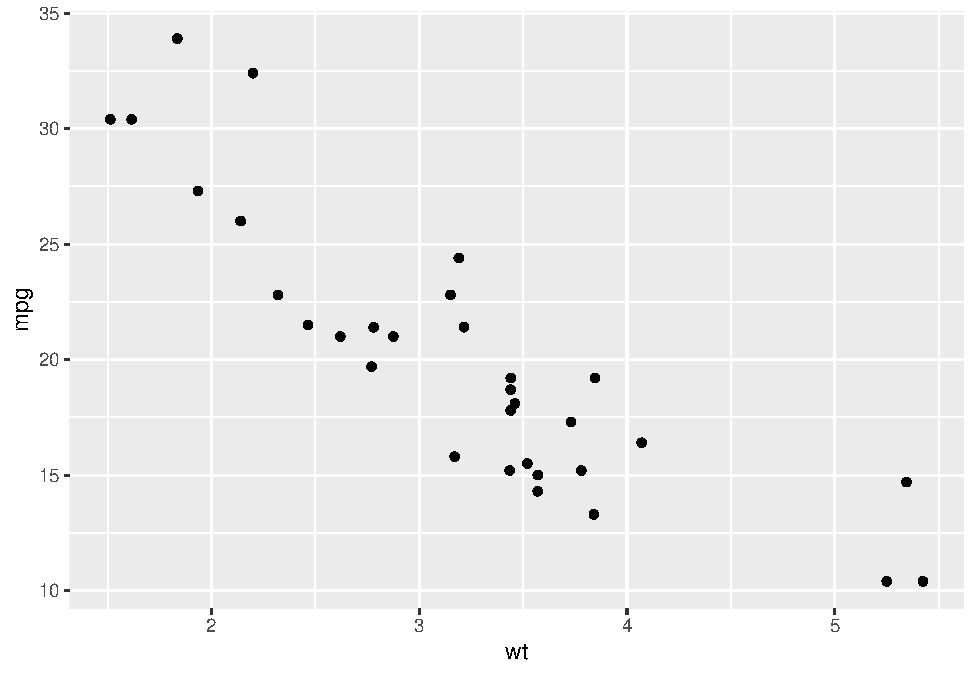
\includegraphics{psych-stats-book_files/figure-latex/unnamed-chunk-57-1.pdf}

In the ggplot2 version, you immediately see the use of aesthetics (\texttt{aes}) to map the variables, and the plot is constructed in layers. This layered approach is central to the power and flexibility of ggplot2.

\hypertarget{installing-and-loading-ggplot2}{%
\subsubsection{Installing and Loading ggplot2}\label{installing-and-loading-ggplot2}}

Before you can start using ggplot2, you need to install the package and load it into your R session.

\begin{enumerate}
\def\labelenumi{\arabic{enumi}.}
\tightlist
\item
  \textbf{Installing ggplot2}:

  \begin{itemize}
  \tightlist
  \item
    If you haven't installed ggplot2 yet, you can do so using the \texttt{install.packages()} function. This downloads the package from CRAN (The Comprehensive R Archive Network) and installs it on your computer.
  \end{itemize}
\end{enumerate}

\begin{Shaded}
\begin{Highlighting}[]
   \FunctionTok{install.packages}\NormalTok{(}\StringTok{"ggplot2"}\NormalTok{)}
\end{Highlighting}
\end{Shaded}

\begin{itemize}
\tightlist
\item
  Once installed, you only need to install ggplot2 once. After installation, you can load it into your R session whenever you need to use it.
\end{itemize}

\begin{enumerate}
\def\labelenumi{\arabic{enumi}.}
\setcounter{enumi}{1}
\tightlist
\item
  \textbf{Loading ggplot2}:

  \begin{itemize}
  \tightlist
  \item
    To use ggplot2 in your R session, load it with the \texttt{library()} function:
  \end{itemize}
\end{enumerate}

\begin{Shaded}
\begin{Highlighting}[]
   \FunctionTok{library}\NormalTok{(ggplot2)}
\end{Highlighting}
\end{Shaded}

\begin{itemize}
\tightlist
\item
  Loading the package makes all its functions available for use. You'll know ggplot2 is loaded correctly if you can start typing ggplot2 functions (like \texttt{ggplot()}) without receiving an error.
\end{itemize}

\begin{enumerate}
\def\labelenumi{\arabic{enumi}.}
\setcounter{enumi}{2}
\tightlist
\item
  \textbf{Integration with the R Ecosystem}:

  \begin{itemize}
  \tightlist
  \item
    ggplot2 is part of the larger tidyverse, a collection of R packages designed for data science. The tidyverse includes packages like dplyr for data manipulation and tidyr for data tidying, which integrate seamlessly with ggplot2. This means you can easily prepare your data with dplyr and then visualize it with ggplot2 in a smooth, cohesive workflow.
  \end{itemize}
\end{enumerate}

\hypertarget{understanding-the-grammar-of-graphics}{%
\subsection{Understanding the Grammar of Graphics}\label{understanding-the-grammar-of-graphics}}

One of the most powerful concepts behind ggplot2 is the ``Grammar of Graphics,'' a systematic way of describing and building plots.

\begin{enumerate}
\def\labelenumi{\arabic{enumi}.}
\tightlist
\item
  \textbf{Aesthetics (\texttt{aes})}:

  \begin{itemize}
  \tightlist
  \item
    Aesthetics are the visual properties of your plot, such as the position of points, colors, shapes, and sizes. In ggplot2, you map your data to these aesthetics using the \texttt{aes()} function. For example:
  \end{itemize}
\end{enumerate}

\begin{Shaded}
\begin{Highlighting}[]
   \FunctionTok{ggplot}\NormalTok{(mtcars, }\FunctionTok{aes}\NormalTok{(}\AttributeTok{x =}\NormalTok{ wt, }\AttributeTok{y =}\NormalTok{ mpg))}
\end{Highlighting}
\end{Shaded}

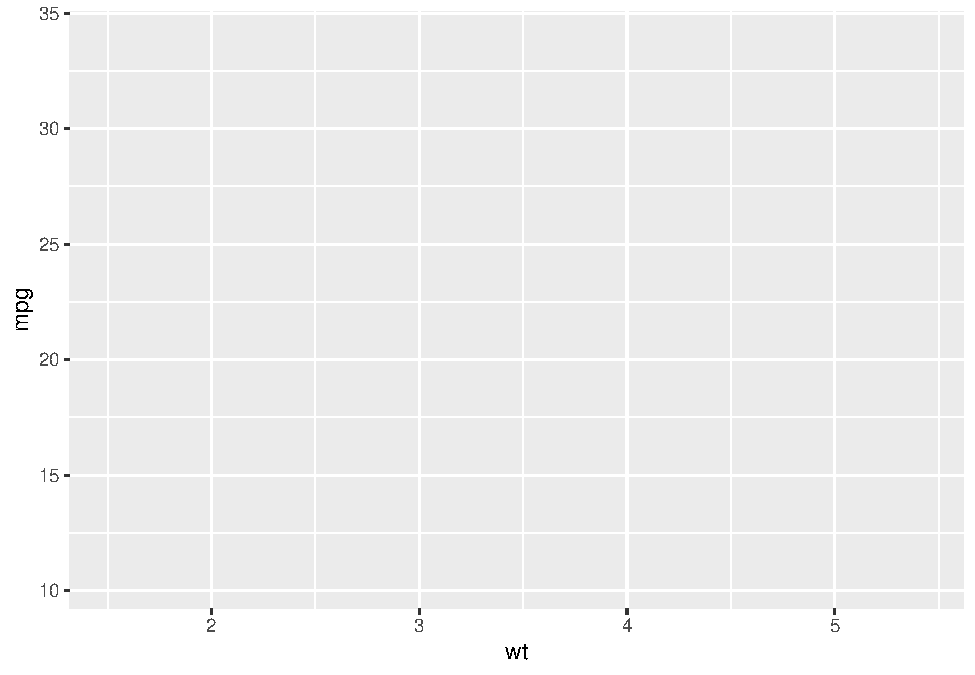
\includegraphics{psych-stats-book_files/figure-latex/unnamed-chunk-60-1.pdf}

\begin{itemize}
\tightlist
\item
  Here, the x-axis is mapped to \texttt{wt} (weight), and the y-axis is mapped to \texttt{mpg} (miles per gallon). This mapping is fundamental to all ggplot2 plots.
\end{itemize}

\begin{enumerate}
\def\labelenumi{\arabic{enumi}.}
\setcounter{enumi}{1}
\tightlist
\item
  \textbf{Layers}:

  \begin{itemize}
  \tightlist
  \item
    ggplot2 builds plots in layers. The first layer typically includes the data and aesthetic mappings, and additional layers can include geometric objects (geoms), statistical transformations, and more. Each layer is added to the plot using the \texttt{+} operator.
  \item
    For example, to add points to a scatter plot, you use the \texttt{geom\_point()} function:
  \end{itemize}
\end{enumerate}

\begin{Shaded}
\begin{Highlighting}[]
   \FunctionTok{ggplot}\NormalTok{(mtcars, }\FunctionTok{aes}\NormalTok{(}\AttributeTok{x =}\NormalTok{ wt, }\AttributeTok{y =}\NormalTok{ mpg)) }\SpecialCharTok{+}
     \FunctionTok{geom\_point}\NormalTok{()}
\end{Highlighting}
\end{Shaded}

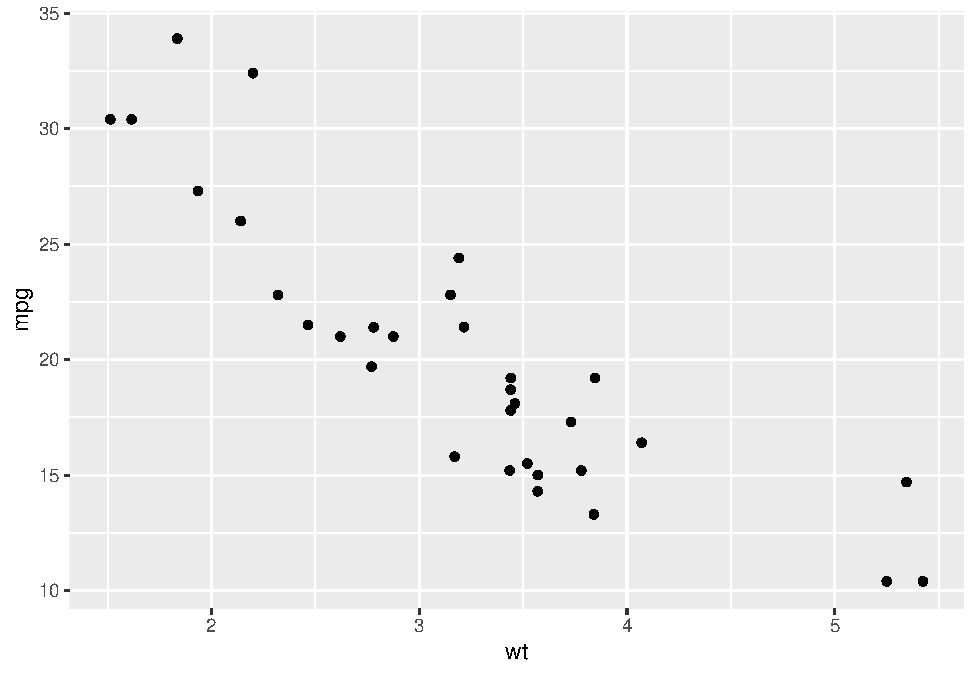
\includegraphics{psych-stats-book_files/figure-latex/unnamed-chunk-61-1.pdf}

\begin{enumerate}
\def\labelenumi{\arabic{enumi}.}
\setcounter{enumi}{2}
\tightlist
\item
  \textbf{Geoms}:

  \begin{itemize}
  \tightlist
  \item
    Geoms are the geometric objects that represent the data in your plot. Common geoms include:

    \begin{itemize}
    \tightlist
    \item
      \texttt{geom\_point()}: For scatter plots.
    \item
      \texttt{geom\_bar()}: For bar charts.
    \item
      \texttt{geom\_line()}: For line graphs.
    \end{itemize}
  \item
    Each geom can be customized by mapping aesthetics or adding specific arguments.
  \end{itemize}
\item
  \textbf{Scales}:

  \begin{itemize}
  \tightlist
  \item
    Scales control how data values are mapped to aesthetic properties, such as the axes or colors. For example, you can adjust the scales of your axes or use different color scales to represent data:
  \end{itemize}
\end{enumerate}

\begin{Shaded}
\begin{Highlighting}[]
   \FunctionTok{ggplot}\NormalTok{(mtcars, }\FunctionTok{aes}\NormalTok{(}\AttributeTok{x =}\NormalTok{ wt, }\AttributeTok{y =}\NormalTok{ mpg)) }\SpecialCharTok{+}
     \FunctionTok{geom\_point}\NormalTok{() }\SpecialCharTok{+}
     \FunctionTok{scale\_x\_continuous}\NormalTok{(}\AttributeTok{limits =} \FunctionTok{c}\NormalTok{(}\DecValTok{0}\NormalTok{, }\DecValTok{6}\NormalTok{))}
\end{Highlighting}
\end{Shaded}

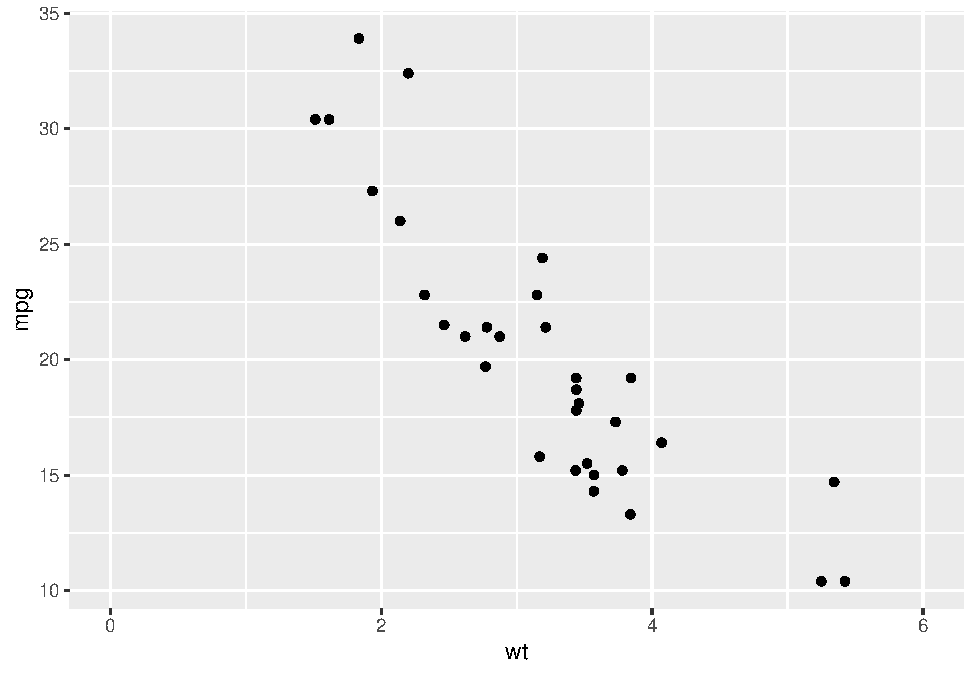
\includegraphics{psych-stats-book_files/figure-latex/unnamed-chunk-62-1.pdf}

\begin{itemize}
\tightlist
\item
  This example sets the x-axis to range from 0 to 6.
\end{itemize}

\begin{enumerate}
\def\labelenumi{\arabic{enumi}.}
\setcounter{enumi}{4}
\tightlist
\item
  \textbf{Facets}:

  \begin{itemize}
  \tightlist
  \item
    Faceting is a way to split your data into multiple plots based on a categorical variable. This is particularly useful when you want to compare different groups side by side. For example, you can create small multiples by faceting by the number of cylinders in the \texttt{mtcars} dataset:
  \end{itemize}
\end{enumerate}

\begin{Shaded}
\begin{Highlighting}[]
   \FunctionTok{ggplot}\NormalTok{(mtcars, }\FunctionTok{aes}\NormalTok{(}\AttributeTok{x =}\NormalTok{ wt, }\AttributeTok{y =}\NormalTok{ mpg)) }\SpecialCharTok{+}
     \FunctionTok{geom\_point}\NormalTok{() }\SpecialCharTok{+}
     \FunctionTok{facet\_wrap}\NormalTok{(}\SpecialCharTok{\textasciitilde{}}\NormalTok{ cyl)}
\end{Highlighting}
\end{Shaded}

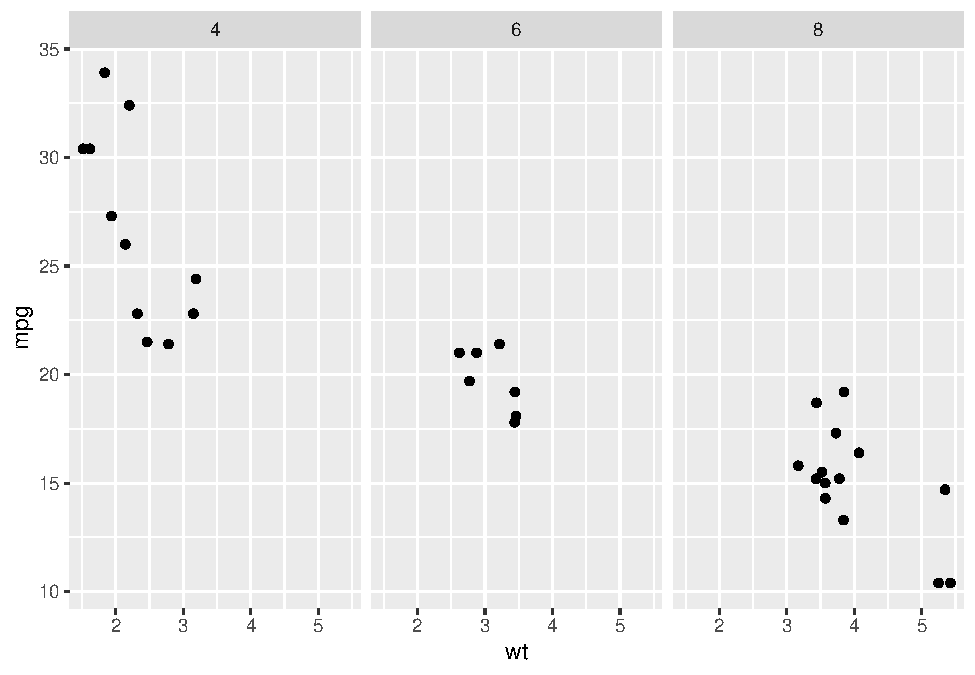
\includegraphics{psych-stats-book_files/figure-latex/unnamed-chunk-63-1.pdf}

\begin{itemize}
\tightlist
\item
  This code will produce separate scatter plots for cars with different numbers of cylinders.
\end{itemize}

\hypertarget{basic-components-of-a-ggplot2-plot}{%
\subsection{Basic Components of a ggplot2 Plot}\label{basic-components-of-a-ggplot2-plot}}

To create a plot in ggplot2, you combine the following components:

\begin{enumerate}
\def\labelenumi{\arabic{enumi}.}
\tightlist
\item
  \textbf{Data}:

  \begin{itemize}
  \tightlist
  \item
    The first step is to prepare your data. Ensure that your data is in a format that ggplot2 can work with, typically a data frame or tibble. The variables you want to plot should be in columns.
  \end{itemize}
\item
  \textbf{Aesthetics (\texttt{aes})}:

  \begin{itemize}
  \tightlist
  \item
    Aesthetics define how your data is visually represented. This involves mapping your data columns to visual properties like the x and y positions, colors, or sizes.
  \end{itemize}
\item
  \textbf{Geoms}:

  \begin{itemize}
  \tightlist
  \item
    Geoms are the shapes or objects that appear on your plot, representing your data points. The choice of geom depends on the type of plot you want to create (e.g., points for scatter plots, bars for bar charts).
  \end{itemize}
\item
  \textbf{Scales}:

  \begin{itemize}
  \tightlist
  \item
    Scales adjust how data is mapped to aesthetics. You can customize the scales of your axes, colors, or sizes to improve the readability and appearance of your plot.
  \end{itemize}
\item
  \textbf{Facets}:

  \begin{itemize}
  \tightlist
  \item
    Faceting allows you to create multiple plots based on a categorical variable, helping to compare different subsets of your data within the same graphic.
  \end{itemize}
\end{enumerate}

\hypertarget{creating-your-first-plot}{%
\subsection{Creating Your First Plot}\label{creating-your-first-plot}}

Let's walk through creating a simple scatter plot using ggplot2.

\begin{enumerate}
\def\labelenumi{\arabic{enumi}.}
\tightlist
\item
  \textbf{Step 1: Prepare Your Data}

  \begin{itemize}
  \tightlist
  \item
    We'll use the built-in \texttt{mtcars} dataset in R, which contains data on different car models, including their weight (\texttt{wt}) and miles per gallon (\texttt{mpg}).
  \end{itemize}
\item
  \textbf{Step 2: Initialize the ggplot Object}

  \begin{itemize}
  \tightlist
  \item
    The first step in creating a plot is to initialize the ggplot object and specify the data and aesthetics:
  \end{itemize}
\end{enumerate}

\begin{Shaded}
\begin{Highlighting}[]
\NormalTok{   p }\OtherTok{\textless{}{-}} \FunctionTok{ggplot}\NormalTok{(mtcars, }\FunctionTok{aes}\NormalTok{(}\AttributeTok{x =}\NormalTok{ wt, }\AttributeTok{y =}\NormalTok{ mpg))}
\end{Highlighting}
\end{Shaded}

\begin{enumerate}
\def\labelenumi{\arabic{enumi}.}
\setcounter{enumi}{2}
\tightlist
\item
  \textbf{Step 3: Add a Geom Layer}

  \begin{itemize}
  \tightlist
  \item
    Next, add a geom to represent your data. For a scatter plot, we use \texttt{geom\_point()}:
  \end{itemize}
\end{enumerate}

\begin{Shaded}
\begin{Highlighting}[]
\NormalTok{   p }\OtherTok{\textless{}{-}}\NormalTok{ p }\SpecialCharTok{+} \FunctionTok{geom\_point}\NormalTok{()}
\end{Highlighting}
\end{Shaded}

\begin{enumerate}
\def\labelenumi{\arabic{enumi}.}
\setcounter{enumi}{3}
\tightlist
\item
  \textbf{Step 4: Customize the Plot}

  \begin{itemize}
  \tightlist
  \item
    You can now customize the plot by adding labels, adjusting scales, or applying a theme:
  \end{itemize}
\end{enumerate}

\begin{Shaded}
\begin{Highlighting}[]
\NormalTok{   p }\OtherTok{\textless{}{-}}\NormalTok{ p }\SpecialCharTok{+} \FunctionTok{labs}\NormalTok{(}\AttributeTok{title =} \StringTok{"Scatter Plot of Weight vs. MPG"}\NormalTok{,}
                 \AttributeTok{x =} \StringTok{"Weight (1000 lbs)"}\NormalTok{,}
                 \AttributeTok{y =} \StringTok{"Miles Per Gallon"}\NormalTok{) }\SpecialCharTok{+}
           \FunctionTok{theme\_minimal}\NormalTok{()}
\end{Highlighting}
\end{Shaded}

\begin{enumerate}
\def\labelenumi{\arabic{enumi}.}
\setcounter{enumi}{4}
\tightlist
\item
  \textbf{Step 5: Display the Plot}

  \begin{itemize}
  \tightlist
  \item
    Finally, display the plot by calling the object:
  \end{itemize}
\end{enumerate}

\begin{Shaded}
\begin{Highlighting}[]
\NormalTok{   p}
\end{Highlighting}
\end{Shaded}

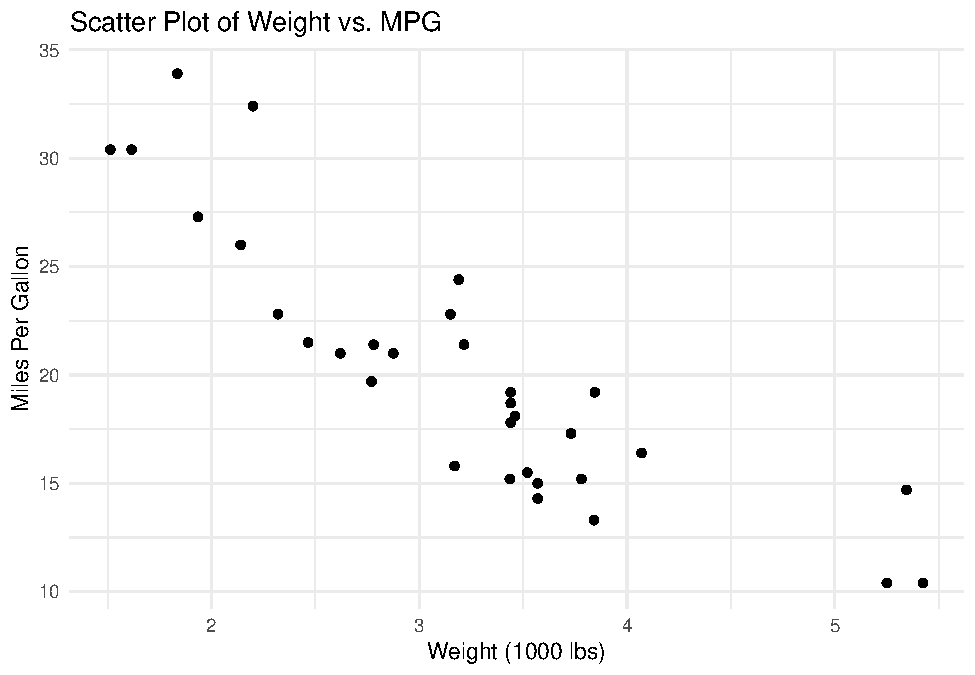
\includegraphics{psych-stats-book_files/figure-latex/unnamed-chunk-67-1.pdf}

\textbf{Example Output}:

The resulting plot will display a scatter plot showing the relationship between the weight of cars and their fuel efficiency. You can see how easy it is to create and customize a plot with ggplot2, even for someone with no prior graphing experience.

\hypertarget{customizing-plots-with-ggplot2}{%
\section{Customizing Plots with ggplot2}\label{customizing-plots-with-ggplot2}}

Once you've created a basic plot in ggplot2, the next step is to customize it to make sure it communicates your message effectively. Customization not only enhances the visual appeal of your plots but also ensures that the information is presented clearly. This section will guide you through the process of adding titles and labels, modifying themes, adjusting colors and styles, adding annotations, and saving your plots.

\hypertarget{adding-titles-and-labels}{%
\subsection{Adding Titles and Labels}\label{adding-titles-and-labels}}

\textbf{Why Titles and Labels Matter}:
Titles and labels are essential for understanding the context of a graph. A well-titled graph with clearly labeled axes makes it easy for the viewer to interpret the data correctly.

\begin{enumerate}
\def\labelenumi{\arabic{enumi}.}
\tightlist
\item
  \textbf{Adding a Title}:

  \begin{itemize}
  \tightlist
  \item
    You can add a title to your plot using the \texttt{labs()} function, where you specify the \texttt{title} argument.
  \item
    Example:
  \end{itemize}
\end{enumerate}

\begin{Shaded}
\begin{Highlighting}[]
     \FunctionTok{ggplot}\NormalTok{(mtcars, }\FunctionTok{aes}\NormalTok{(}\AttributeTok{x =}\NormalTok{ wt, }\AttributeTok{y =}\NormalTok{ mpg)) }\SpecialCharTok{+}
       \FunctionTok{geom\_point}\NormalTok{() }\SpecialCharTok{+}
       \FunctionTok{labs}\NormalTok{(}\AttributeTok{title =} \StringTok{"Relationship Between Weight and MPG"}\NormalTok{)}
\end{Highlighting}
\end{Shaded}

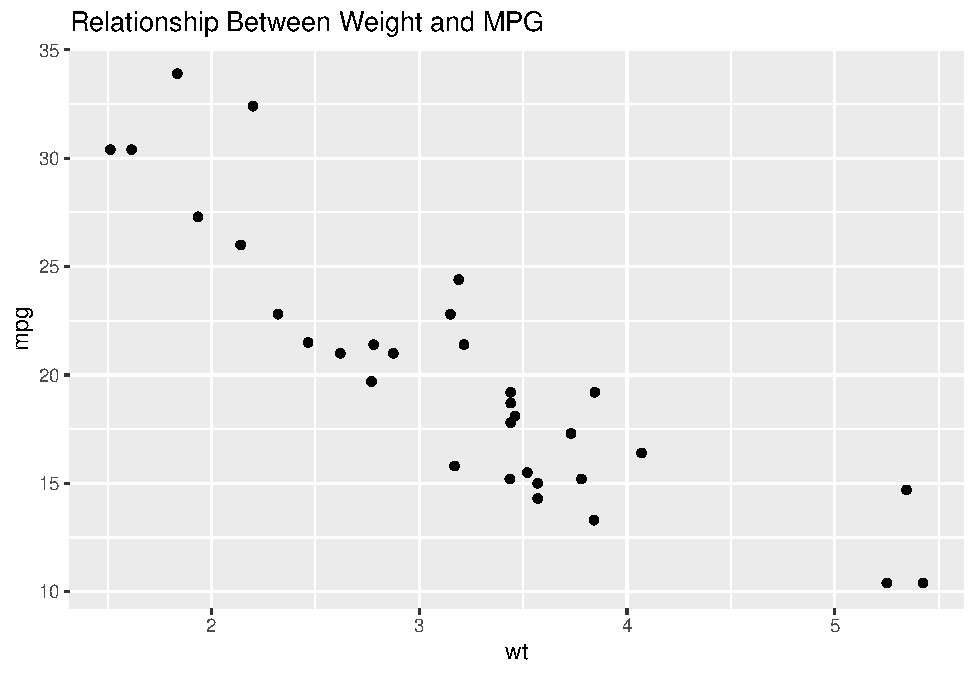
\includegraphics{psych-stats-book_files/figure-latex/unnamed-chunk-68-1.pdf}
- This adds a title at the top of the plot.

\begin{enumerate}
\def\labelenumi{\arabic{enumi}.}
\setcounter{enumi}{1}
\tightlist
\item
  \textbf{Adding Axis Labels}:

  \begin{itemize}
  \tightlist
  \item
    Axis labels help the viewer understand what the axes represent. You can add labels for the x and y axes using the \texttt{labs()} function.
  \item
    Example:
  \end{itemize}
\end{enumerate}

\begin{Shaded}
\begin{Highlighting}[]
     \FunctionTok{ggplot}\NormalTok{(mtcars, }\FunctionTok{aes}\NormalTok{(}\AttributeTok{x =}\NormalTok{ wt, }\AttributeTok{y =}\NormalTok{ mpg)) }\SpecialCharTok{+}
       \FunctionTok{geom\_point}\NormalTok{() }\SpecialCharTok{+}
       \FunctionTok{labs}\NormalTok{(}\AttributeTok{title =} \StringTok{"Relationship Between Weight and MPG"}\NormalTok{,}
            \AttributeTok{x =} \StringTok{"Weight (1000 lbs)"}\NormalTok{,}
            \AttributeTok{y =} \StringTok{"Miles Per Gallon"}\NormalTok{)}
\end{Highlighting}
\end{Shaded}

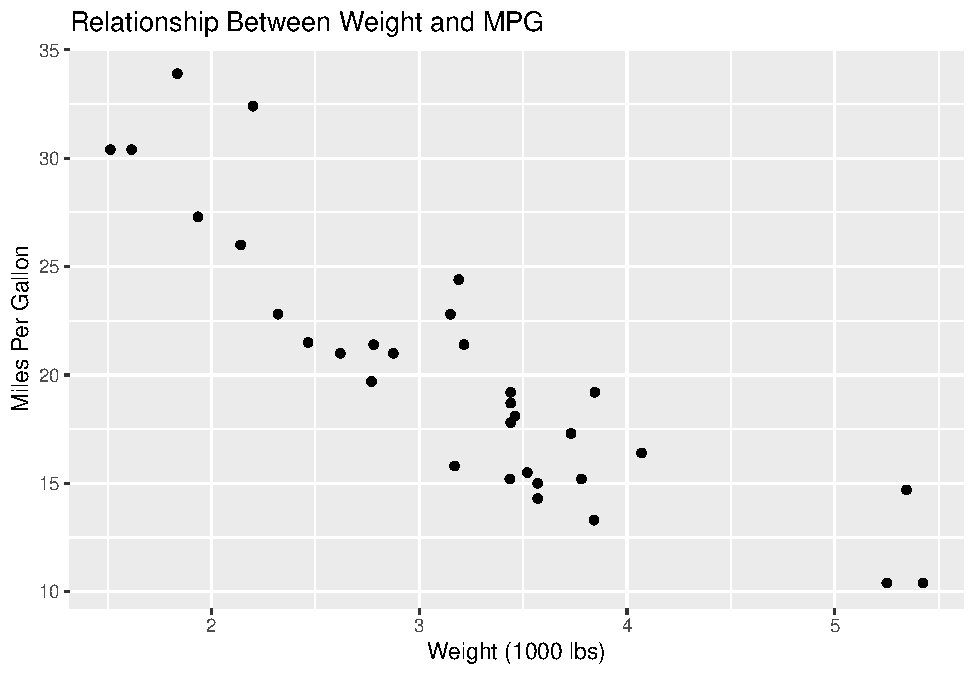
\includegraphics{psych-stats-book_files/figure-latex/unnamed-chunk-69-1.pdf}
- Here, \texttt{x} and \texttt{y} specify the labels for the x and y axes, respectively.

\begin{enumerate}
\def\labelenumi{\arabic{enumi}.}
\setcounter{enumi}{2}
\tightlist
\item
  \textbf{Customizing Legends}:

  \begin{itemize}
  \tightlist
  \item
    Legends are used when you have multiple groups or categories in your plot. You can customize the legend title and labels within the \texttt{labs()} function.
  \item
    Example:
  \end{itemize}
\end{enumerate}

\begin{Shaded}
\begin{Highlighting}[]
     \FunctionTok{ggplot}\NormalTok{(mtcars, }\FunctionTok{aes}\NormalTok{(}\AttributeTok{x =}\NormalTok{ wt, }\AttributeTok{y =}\NormalTok{ mpg, }\AttributeTok{color =} \FunctionTok{factor}\NormalTok{(cyl))) }\SpecialCharTok{+}
       \FunctionTok{geom\_point}\NormalTok{() }\SpecialCharTok{+}
       \FunctionTok{labs}\NormalTok{(}\AttributeTok{title =} \StringTok{"MPG by Car Weight and Cylinders"}\NormalTok{,}
            \AttributeTok{x =} \StringTok{"Weight (1000 lbs)"}\NormalTok{,}
            \AttributeTok{y =} \StringTok{"Miles Per Gallon"}\NormalTok{,}
            \AttributeTok{color =} \StringTok{"Number of Cylinders"}\NormalTok{)}
\end{Highlighting}
\end{Shaded}

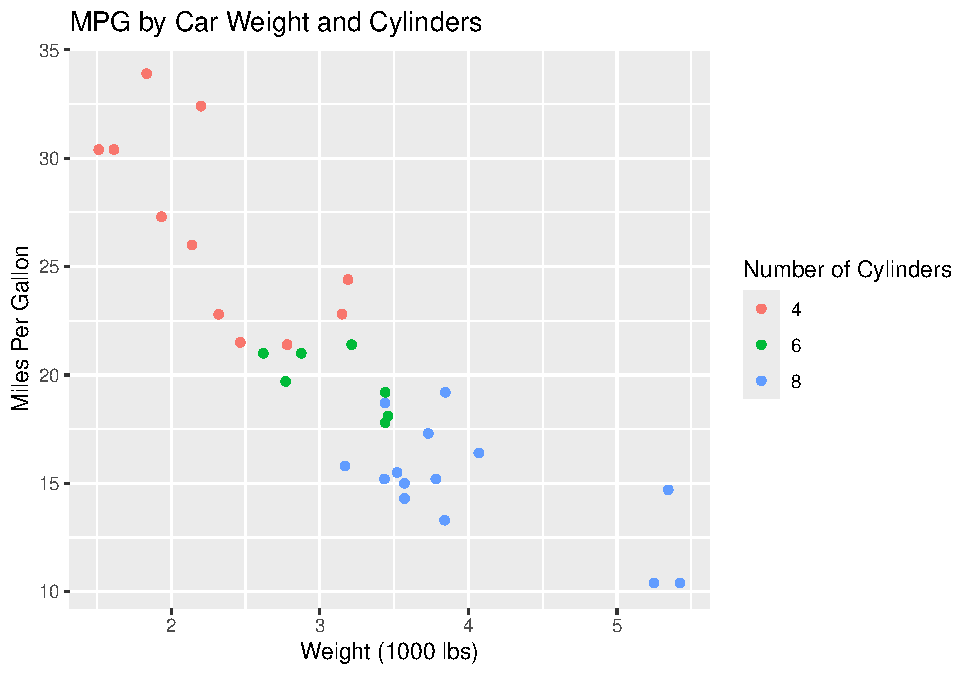
\includegraphics{psych-stats-book_files/figure-latex/unnamed-chunk-70-1.pdf}
- In this example, the \texttt{color} argument within \texttt{labs()} changes the legend title to ``Number of Cylinders.''

\begin{enumerate}
\def\labelenumi{\arabic{enumi}.}
\setcounter{enumi}{3}
\tightlist
\item
  \textbf{Positioning Titles and Labels}:

  \begin{itemize}
  \tightlist
  \item
    You can adjust the position of titles and labels using the \texttt{theme()} function. For instance, to center the plot title:
  \end{itemize}
\end{enumerate}

\begin{Shaded}
\begin{Highlighting}[]
   \FunctionTok{ggplot}\NormalTok{(mtcars, }\FunctionTok{aes}\NormalTok{(}\AttributeTok{x =}\NormalTok{ wt, }\AttributeTok{y =}\NormalTok{ mpg)) }\SpecialCharTok{+}
     \FunctionTok{geom\_point}\NormalTok{() }\SpecialCharTok{+}
     \FunctionTok{labs}\NormalTok{(}\AttributeTok{title =} \StringTok{"Relationship Between Weight and MPG"}\NormalTok{,}
          \AttributeTok{x =} \StringTok{"Weight (1000 lbs)"}\NormalTok{,}
          \AttributeTok{y =} \StringTok{"Miles Per Gallon"}\NormalTok{) }\SpecialCharTok{+}
     \FunctionTok{theme}\NormalTok{(}\AttributeTok{plot.title =} \FunctionTok{element\_text}\NormalTok{(}\AttributeTok{hjust =} \FloatTok{0.5}\NormalTok{))}
\end{Highlighting}
\end{Shaded}

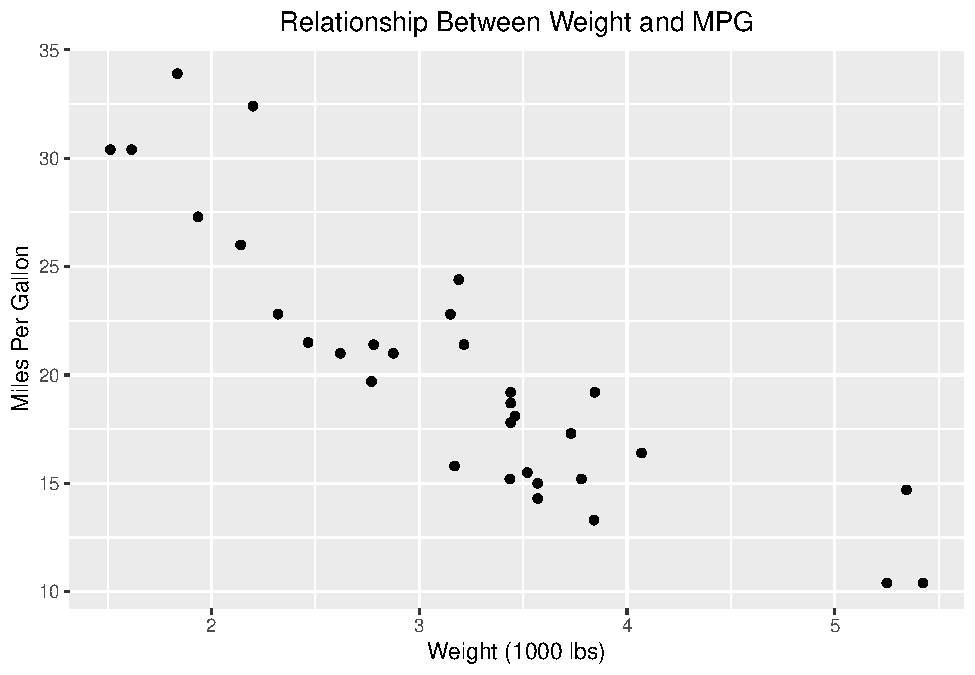
\includegraphics{psych-stats-book_files/figure-latex/unnamed-chunk-71-1.pdf}
- The \texttt{hjust} parameter (horizontal justification) controls the alignment of the title (0 = left, 0.5 = center, 1 = right).

\hypertarget{modifying-themes}{%
\subsection{Modifying Themes}\label{modifying-themes}}

\textbf{What Are Themes?}:
Themes control the overall look and feel of your plot, including background color, grid lines, text size, and font. ggplot2 comes with several built-in themes, and you can also create your own.

\begin{enumerate}
\def\labelenumi{\arabic{enumi}.}
\tightlist
\item
  \textbf{Using Pre-Built Themes}:

  \begin{itemize}
  \tightlist
  \item
    ggplot2 provides several pre-built themes that you can apply with a single line of code. Some popular themes include:

    \begin{itemize}
    \tightlist
    \item
      \texttt{theme\_minimal()}: A clean, simple theme with no background color.
    \item
      \texttt{theme\_classic()}: A traditional theme with a white background and black grid lines.
    \item
      \texttt{theme\_light()}: A light, airy theme with soft grid lines.
    \end{itemize}
  \item
    Example:
  \end{itemize}
\end{enumerate}

\begin{Shaded}
\begin{Highlighting}[]
     \FunctionTok{ggplot}\NormalTok{(mtcars, }\FunctionTok{aes}\NormalTok{(}\AttributeTok{x =}\NormalTok{ wt, }\AttributeTok{y =}\NormalTok{ mpg)) }\SpecialCharTok{+}
       \FunctionTok{geom\_point}\NormalTok{() }\SpecialCharTok{+}
       \FunctionTok{theme\_minimal}\NormalTok{()}
\end{Highlighting}
\end{Shaded}

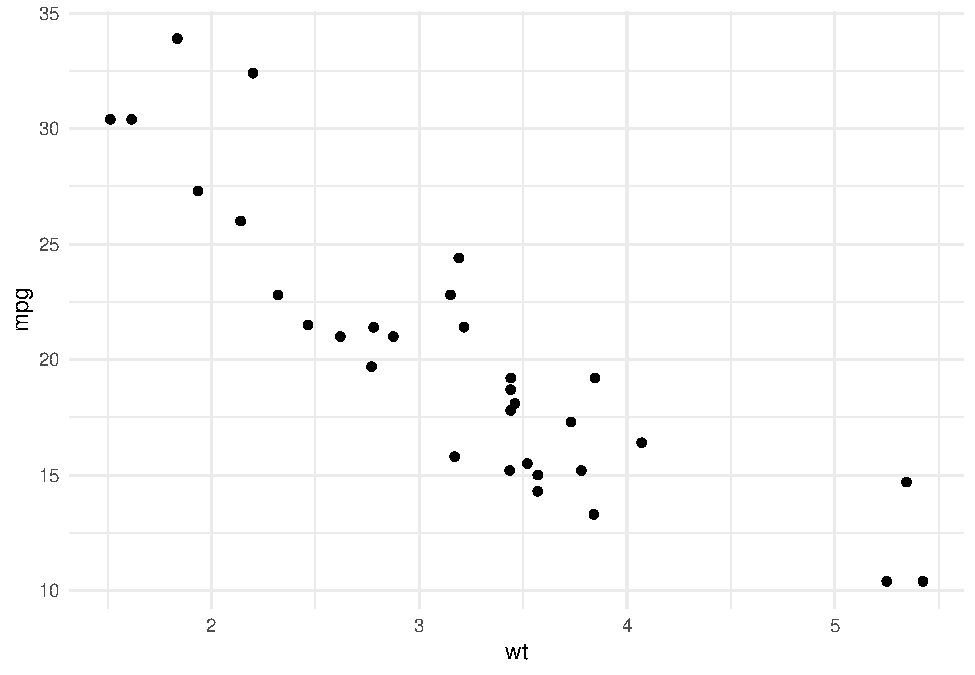
\includegraphics{psych-stats-book_files/figure-latex/unnamed-chunk-72-1.pdf}
- This applies the \texttt{theme\_minimal()} to the plot, resulting in a modern, minimalistic appearance.

\begin{enumerate}
\def\labelenumi{\arabic{enumi}.}
\setcounter{enumi}{1}
\tightlist
\item
  \textbf{Customizing Themes}:

  \begin{itemize}
  \tightlist
  \item
    You can modify specific elements of a theme using the \texttt{theme()} function. For example, you might want to change the text size or remove grid lines:
  \item
    Example:
  \end{itemize}
\end{enumerate}

\begin{Shaded}
\begin{Highlighting}[]
     \FunctionTok{ggplot}\NormalTok{(mtcars, }\FunctionTok{aes}\NormalTok{(}\AttributeTok{x =}\NormalTok{ wt, }\AttributeTok{y =}\NormalTok{ mpg)) }\SpecialCharTok{+}
       \FunctionTok{geom\_point}\NormalTok{() }\SpecialCharTok{+}
       \FunctionTok{theme\_minimal}\NormalTok{() }\SpecialCharTok{+}
       \FunctionTok{theme}\NormalTok{(}\AttributeTok{text =} \FunctionTok{element\_text}\NormalTok{(}\AttributeTok{size =} \DecValTok{12}\NormalTok{),}
             \AttributeTok{panel.grid.major =} \FunctionTok{element\_blank}\NormalTok{(),}
             \AttributeTok{panel.grid.minor =} \FunctionTok{element\_blank}\NormalTok{())}
\end{Highlighting}
\end{Shaded}

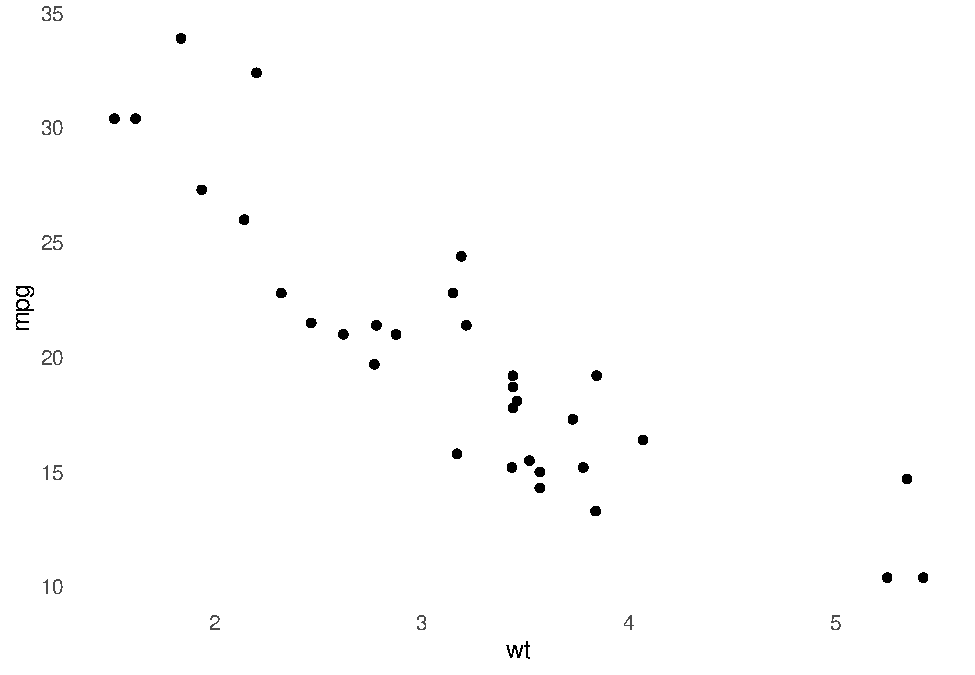
\includegraphics{psych-stats-book_files/figure-latex/unnamed-chunk-73-1.pdf}
- In this example, the text size is increased, and both major and minor grid lines are removed.

\begin{enumerate}
\def\labelenumi{\arabic{enumi}.}
\setcounter{enumi}{2}
\tightlist
\item
  \textbf{Combining Themes}:

  \begin{itemize}
  \tightlist
  \item
    You can layer multiple theme modifications to achieve the desired look. For instance, you might combine \texttt{theme\_classic()} with additional customizations:
  \item
    Example:
  \end{itemize}
\end{enumerate}

\begin{Shaded}
\begin{Highlighting}[]
     \FunctionTok{ggplot}\NormalTok{(mtcars, }\FunctionTok{aes}\NormalTok{(}\AttributeTok{x =}\NormalTok{ wt, }\AttributeTok{y =}\NormalTok{ mpg)) }\SpecialCharTok{+}
       \FunctionTok{geom\_point}\NormalTok{() }\SpecialCharTok{+}
       \FunctionTok{theme\_classic}\NormalTok{() }\SpecialCharTok{+}
       \FunctionTok{theme}\NormalTok{(}\AttributeTok{axis.text =} \FunctionTok{element\_text}\NormalTok{(}\AttributeTok{size =} \DecValTok{10}\NormalTok{, }\AttributeTok{color =} \StringTok{"blue"}\NormalTok{),}
             \AttributeTok{axis.title =} \FunctionTok{element\_text}\NormalTok{(}\AttributeTok{size =} \DecValTok{14}\NormalTok{, }\AttributeTok{face =} \StringTok{"bold"}\NormalTok{))}
\end{Highlighting}
\end{Shaded}

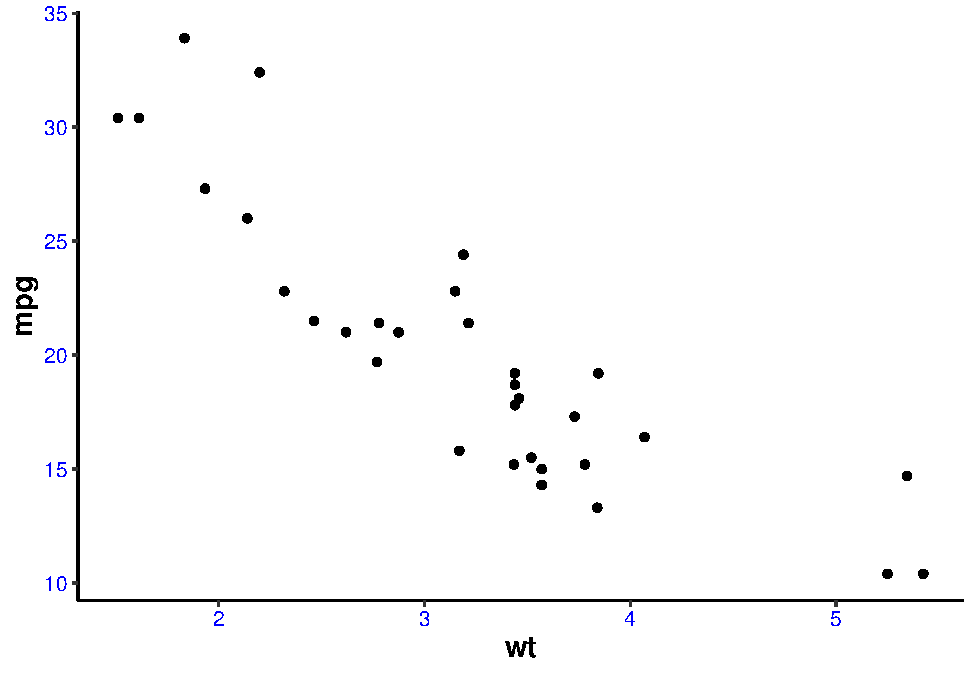
\includegraphics{psych-stats-book_files/figure-latex/unnamed-chunk-74-1.pdf}
- This combines the classic theme with custom axis text and title sizes, and changes the axis text color to blue.

\hypertarget{adjusting-colors-and-styles}{%
\subsection{Adjusting Colors and Styles}\label{adjusting-colors-and-styles}}

\textbf{Why Adjust Colors and Styles?}:
Colors and styles are critical for distinguishing different groups or categories within your plot. Proper use of colors can also make your plots more engaging and easier to interpret.

\begin{enumerate}
\def\labelenumi{\arabic{enumi}.}
\tightlist
\item
  \textbf{Changing Point and Line Colors}:

  \begin{itemize}
  \tightlist
  \item
    You can change the color of points or lines using the \texttt{color} aesthetic. This is particularly useful when you want to differentiate between groups.
  \item
    Example:
  \end{itemize}
\end{enumerate}

\begin{Shaded}
\begin{Highlighting}[]
     \FunctionTok{ggplot}\NormalTok{(mtcars, }\FunctionTok{aes}\NormalTok{(}\AttributeTok{x =}\NormalTok{ wt, }\AttributeTok{y =}\NormalTok{ mpg, }\AttributeTok{color =} \FunctionTok{factor}\NormalTok{(cyl))) }\SpecialCharTok{+}
       \FunctionTok{geom\_point}\NormalTok{(}\AttributeTok{size =} \DecValTok{3}\NormalTok{) }\SpecialCharTok{+}
       \FunctionTok{labs}\NormalTok{(}\AttributeTok{color =} \StringTok{"Cylinders"}\NormalTok{)}
\end{Highlighting}
\end{Shaded}

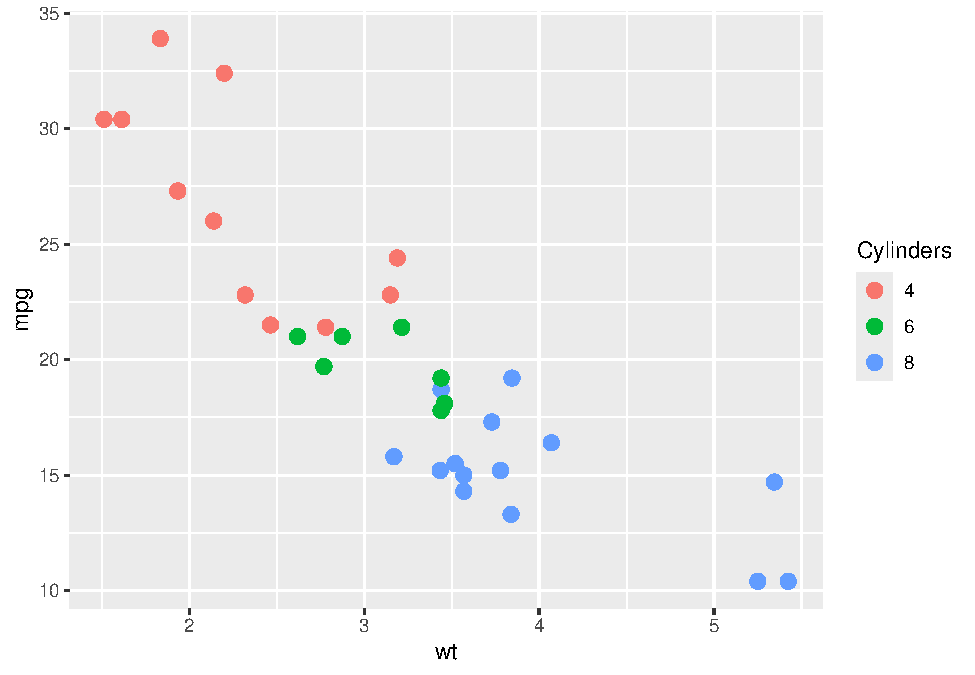
\includegraphics{psych-stats-book_files/figure-latex/unnamed-chunk-75-1.pdf}
- In this example, points are colored based on the number of cylinders, making it easy to see how different cylinder groups perform in terms of MPG.

\begin{enumerate}
\def\labelenumi{\arabic{enumi}.}
\setcounter{enumi}{1}
\tightlist
\item
  \textbf{Customizing Line Types and Point Shapes}:

  \begin{itemize}
  \tightlist
  \item
    Line types (e.g., solid, dashed) and point shapes (e.g., circles, triangles) can also be customized using the \texttt{linetype} and \texttt{shape} aesthetics.
  \item
    Example:
  \end{itemize}
\end{enumerate}

\begin{Shaded}
\begin{Highlighting}[]
     \FunctionTok{ggplot}\NormalTok{(mtcars, }\FunctionTok{aes}\NormalTok{(}\AttributeTok{x =}\NormalTok{ wt, }\AttributeTok{y =}\NormalTok{ mpg, }\AttributeTok{shape =} \FunctionTok{factor}\NormalTok{(cyl))) }\SpecialCharTok{+}
       \FunctionTok{geom\_point}\NormalTok{(}\AttributeTok{size =} \DecValTok{3}\NormalTok{) }\SpecialCharTok{+}
       \FunctionTok{scale\_shape\_manual}\NormalTok{(}\AttributeTok{values =} \FunctionTok{c}\NormalTok{(}\DecValTok{16}\NormalTok{, }\DecValTok{17}\NormalTok{, }\DecValTok{18}\NormalTok{)) }\SpecialCharTok{+}
       \FunctionTok{labs}\NormalTok{(}\AttributeTok{shape =} \StringTok{"Cylinders"}\NormalTok{)}
\end{Highlighting}
\end{Shaded}

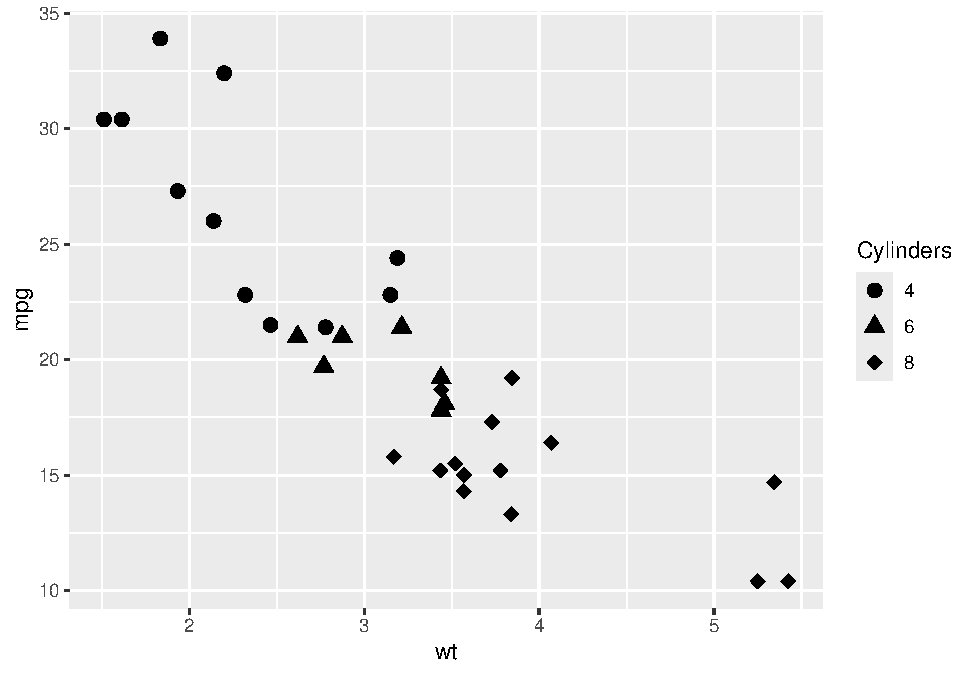
\includegraphics{psych-stats-book_files/figure-latex/unnamed-chunk-76-1.pdf}
- This code assigns different shapes to the points based on the number of cylinders, which can be helpful for differentiating groups.

\begin{enumerate}
\def\labelenumi{\arabic{enumi}.}
\setcounter{enumi}{2}
\tightlist
\item
  \textbf{Using Custom Color Palettes}:

  \begin{itemize}
  \tightlist
  \item
    You can apply custom color palettes using the \texttt{scale\_color\_manual()} function or choose from predefined palettes with \texttt{scale\_color\_brewer()}.
  \item
    Example:
  \end{itemize}
\end{enumerate}

\begin{Shaded}
\begin{Highlighting}[]
     \FunctionTok{ggplot}\NormalTok{(mtcars, }\FunctionTok{aes}\NormalTok{(}\AttributeTok{x =}\NormalTok{ wt, }\AttributeTok{y =}\NormalTok{ mpg, }\AttributeTok{color =} \FunctionTok{factor}\NormalTok{(cyl))) }\SpecialCharTok{+}
       \FunctionTok{geom\_point}\NormalTok{(}\AttributeTok{size =} \DecValTok{3}\NormalTok{) }\SpecialCharTok{+}
       \FunctionTok{scale\_color\_brewer}\NormalTok{(}\AttributeTok{palette =} \StringTok{"Set1"}\NormalTok{) }\SpecialCharTok{+}
       \FunctionTok{labs}\NormalTok{(}\AttributeTok{color =} \StringTok{"Cylinders"}\NormalTok{)}
\end{Highlighting}
\end{Shaded}

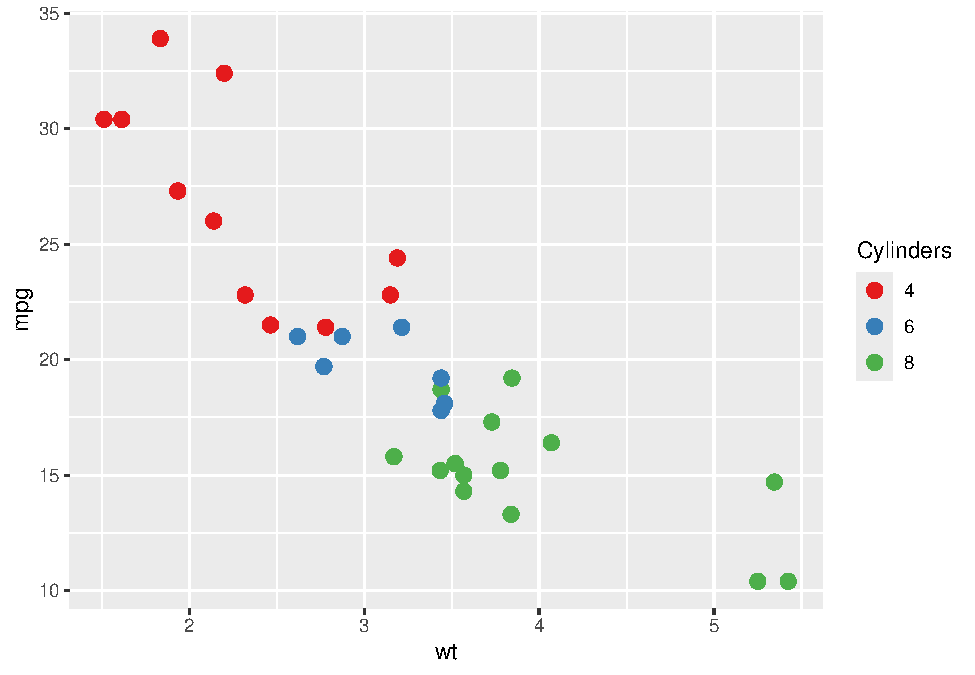
\includegraphics{psych-stats-book_files/figure-latex/unnamed-chunk-77-1.pdf}
- The \texttt{Set1} palette is from the ColorBrewer library, which provides colorblind-friendly palettes.

\hypertarget{adding-annotations}{%
\subsection{Adding Annotations}\label{adding-annotations}}

\textbf{Why Add Annotations?}:
Annotations help to highlight specific data points or add explanatory text to your plot, making it easier to convey the key message.

\begin{enumerate}
\def\labelenumi{\arabic{enumi}.}
\tightlist
\item
  \textbf{Adding Text Annotations}:

  \begin{itemize}
  \tightlist
  \item
    You can add text annotations using the \texttt{annotate()} function or \texttt{geom\_text()} to place text at specific coordinates on the plot.
  \item
    Example:
  \end{itemize}
\end{enumerate}

\begin{Shaded}
\begin{Highlighting}[]
     \FunctionTok{ggplot}\NormalTok{(mtcars, }\FunctionTok{aes}\NormalTok{(}\AttributeTok{x =}\NormalTok{ wt, }\AttributeTok{y =}\NormalTok{ mpg)) }\SpecialCharTok{+}
       \FunctionTok{geom\_point}\NormalTok{() }\SpecialCharTok{+}
       \FunctionTok{annotate}\NormalTok{(}\StringTok{"text"}\NormalTok{, }\AttributeTok{x =} \DecValTok{5}\NormalTok{, }\AttributeTok{y =} \DecValTok{30}\NormalTok{, }\AttributeTok{label =} \StringTok{"High MPG"}\NormalTok{, }\AttributeTok{color =} \StringTok{"red"}\NormalTok{)}
\end{Highlighting}
\end{Shaded}

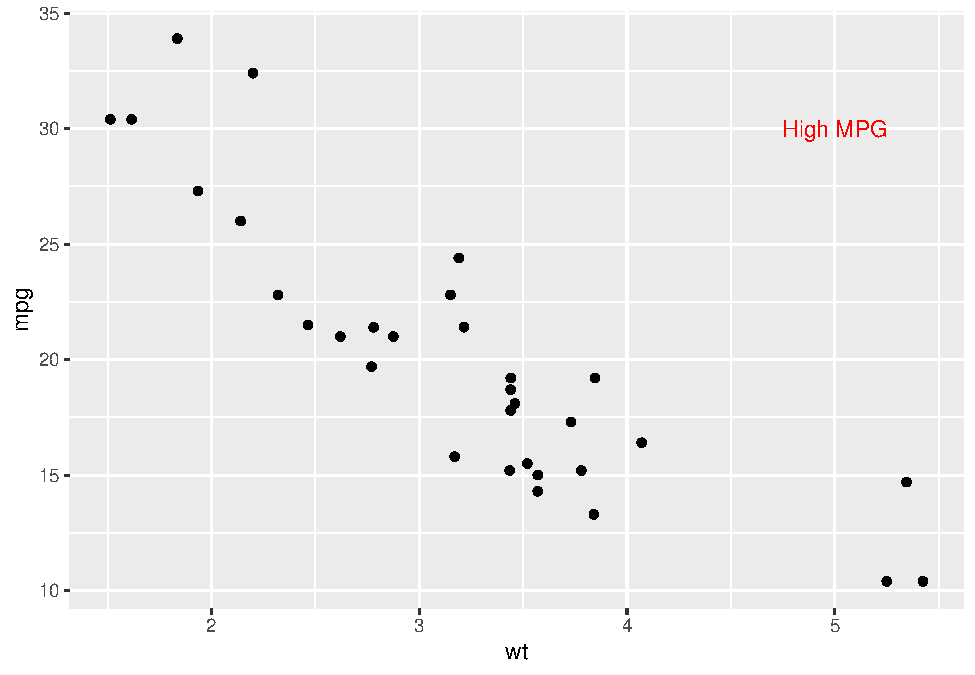
\includegraphics{psych-stats-book_files/figure-latex/unnamed-chunk-78-1.pdf}
- This adds a text label ``High MPG'' at the specified coordinates.

\begin{enumerate}
\def\labelenumi{\arabic{enumi}.}
\setcounter{enumi}{1}
\tightlist
\item
  \textbf{Adding Lines and Rectangles}:

  \begin{itemize}
  \tightlist
  \item
    You can add horizontal or vertical lines using \texttt{geom\_hline()} or \texttt{geom\_vline()}, and shaded rectangles using \texttt{geom\_rect()}.
  \item
    Example:
  \end{itemize}
\end{enumerate}

\begin{Shaded}
\begin{Highlighting}[]
     \FunctionTok{ggplot}\NormalTok{(mtcars, }\FunctionTok{aes}\NormalTok{(}\AttributeTok{x =}\NormalTok{ wt, }\AttributeTok{y =}\NormalTok{ mpg)) }\SpecialCharTok{+}
       \FunctionTok{geom\_point}\NormalTok{() }\SpecialCharTok{+}
       \FunctionTok{geom\_hline}\NormalTok{(}\AttributeTok{yintercept =} \DecValTok{20}\NormalTok{, }\AttributeTok{linetype =} \StringTok{"dashed"}\NormalTok{, }\AttributeTok{color =} \StringTok{"blue"}\NormalTok{) }\SpecialCharTok{+}
       \FunctionTok{geom\_vline}\NormalTok{(}\AttributeTok{xintercept =} \DecValTok{4}\NormalTok{, }\AttributeTok{linetype =} \StringTok{"dashed"}\NormalTok{, }\AttributeTok{color =} \StringTok{"blue"}\NormalTok{)}
\end{Highlighting}
\end{Shaded}

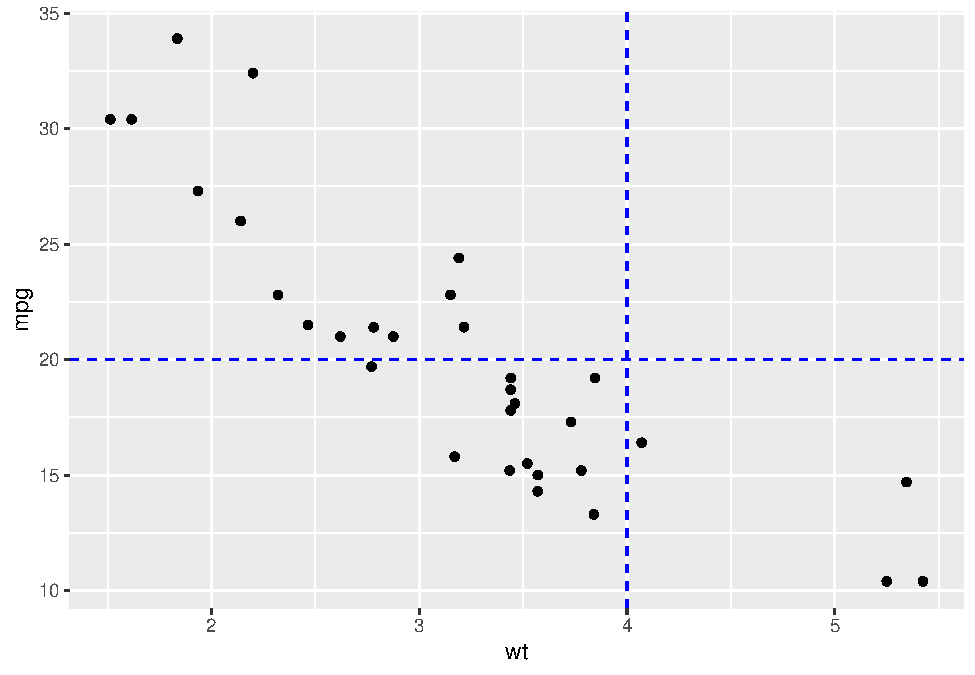
\includegraphics{psych-stats-book_files/figure-latex/unnamed-chunk-79-1.pdf}
- This adds dashed lines at y = 20 and x = 4, helping to highlight specific areas of the plot.

\begin{enumerate}
\def\labelenumi{\arabic{enumi}.}
\setcounter{enumi}{2}
\tightlist
\item
  \textbf{Adding Arrows and Segments}:

  \begin{itemize}
  \tightlist
  \item
    Use \texttt{geom\_segment()} to add arrows or line segments to draw attention to specific parts of the plot.
  \item
    Example:
  \end{itemize}
\end{enumerate}

\begin{Shaded}
\begin{Highlighting}[]
     \FunctionTok{ggplot}\NormalTok{(mtcars, }\FunctionTok{aes}\NormalTok{(}\AttributeTok{x =}\NormalTok{ wt, }\AttributeTok{y =}\NormalTok{ mpg)) }\SpecialCharTok{+}
       \FunctionTok{geom\_point}\NormalTok{() }\SpecialCharTok{+}
       \FunctionTok{geom\_segment}\NormalTok{(}\FunctionTok{aes}\NormalTok{(}\AttributeTok{x =} \DecValTok{4}\NormalTok{, }\AttributeTok{y =} \DecValTok{15}\NormalTok{, }\AttributeTok{xend =} \DecValTok{5}\NormalTok{, }\AttributeTok{yend =} \DecValTok{20}\NormalTok{),}
                    \AttributeTok{arrow =} \FunctionTok{arrow}\NormalTok{(}\AttributeTok{length =} \FunctionTok{unit}\NormalTok{(}\FloatTok{0.3}\NormalTok{, }\StringTok{"cm"}\NormalTok{)),}
                    \AttributeTok{color =} \StringTok{"green"}\NormalTok{)}
\end{Highlighting}
\end{Shaded}

\begin{verbatim}
## Warning in geom_segment(aes(x = 4, y = 15, xend = 5, yend = 20), arrow = arrow(length = unit(0.3, : All aesthetics have length 1, but the data has 32 rows.
## i Please consider using `annotate()` or provide this layer with data
##   containing a single row.
\end{verbatim}

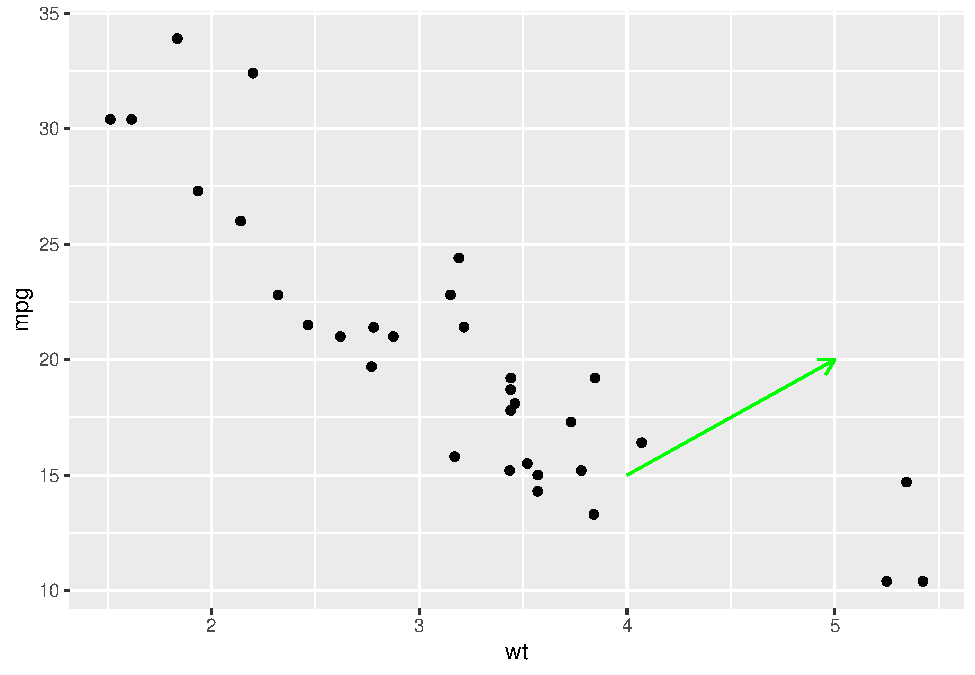
\includegraphics{psych-stats-book_files/figure-latex/unnamed-chunk-80-1.pdf}
- This draws an arrow from (4, 15) to (5, 20), pointing out a specific trend or relationship in the data.

\hypertarget{saving-and-exporting-plots}{%
\section{Saving and Exporting Plots}\label{saving-and-exporting-plots}}

\textbf{Why Save Plots?}:
Saving your plots allows you to include them in reports, presentations, or publications. You can save plots in various formats, such as PNG, PDF, or JPEG, depending on your needs.

Certainly! Let's continue with the section on saving and exporting plots in ggplot2.

\hypertarget{saving-and-exporting-plots-1}{%
\subsection{Saving and Exporting Plots}\label{saving-and-exporting-plots-1}}

\textbf{Why Save Plots?}:
Saving your plots allows you to include them in reports, presentations, or publications. You can save plots in various formats, such as PNG, PDF, or JPEG, depending on your needs. ggplot2 makes it easy to save your plots with high resolution and in different sizes.

\begin{enumerate}
\def\labelenumi{\arabic{enumi}.}
\tightlist
\item
  \textbf{Saving Plots as Image Files}:

  \begin{itemize}
  \tightlist
  \item
    The \texttt{ggsave()} function is the most common way to save plots in ggplot2. It automatically saves the last plot you created, but you can also specify a plot to save by passing it as an argument.
  \item
    Example: Saving as a PNG file
  \end{itemize}
\end{enumerate}

\begin{Shaded}
\begin{Highlighting}[]
     \FunctionTok{ggplot}\NormalTok{(mtcars, }\FunctionTok{aes}\NormalTok{(}\AttributeTok{x =}\NormalTok{ wt, }\AttributeTok{y =}\NormalTok{ mpg)) }\SpecialCharTok{+}
       \FunctionTok{geom\_point}\NormalTok{() }\SpecialCharTok{+}
       \FunctionTok{labs}\NormalTok{(}\AttributeTok{title =} \StringTok{"Relationship Between Weight and MPG"}\NormalTok{)}
\end{Highlighting}
\end{Shaded}

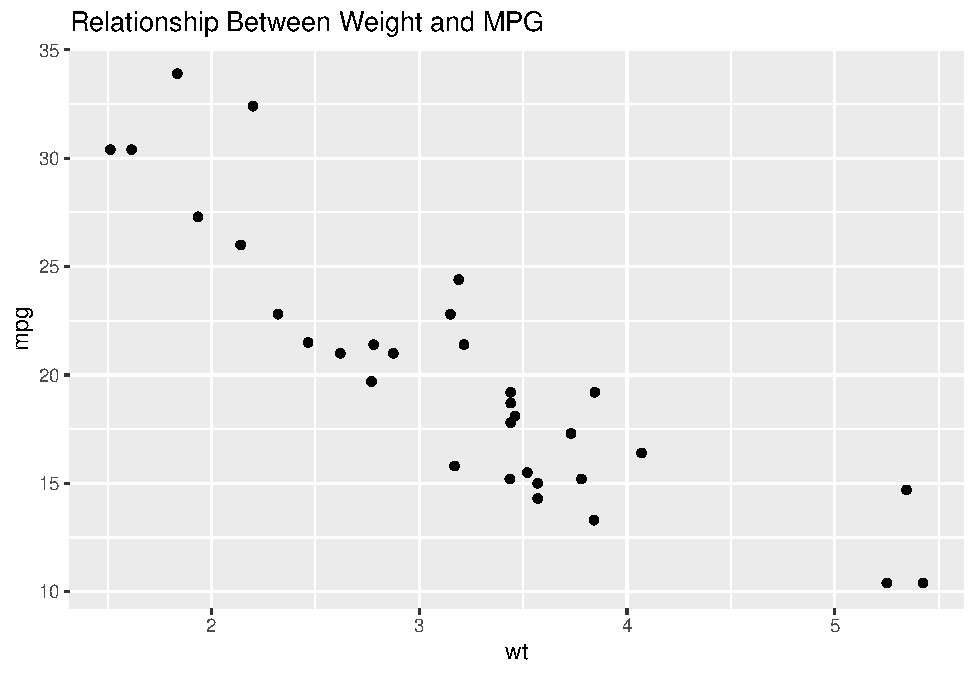
\includegraphics{psych-stats-book_files/figure-latex/unnamed-chunk-81-1.pdf}

\begin{Shaded}
\begin{Highlighting}[]
     \FunctionTok{ggsave}\NormalTok{(}\StringTok{"weight\_vs\_mpg.png"}\NormalTok{, }\AttributeTok{width =} \DecValTok{6}\NormalTok{, }\AttributeTok{height =} \DecValTok{4}\NormalTok{, }\AttributeTok{dpi =} \DecValTok{300}\NormalTok{)}
\end{Highlighting}
\end{Shaded}

\begin{itemize}
\tightlist
\item
  In this example, the plot is saved as a PNG file named ``weight\_vs\_mpg.png''. The \texttt{width} and \texttt{height} parameters control the size of the image, and \texttt{dpi} (dots per inch) controls the resolution (300 dpi is standard for high-quality images).
\end{itemize}

\begin{enumerate}
\def\labelenumi{\arabic{enumi}.}
\setcounter{enumi}{1}
\tightlist
\item
  \textbf{Saving Plots as PDF Files}:

  \begin{itemize}
  \tightlist
  \item
    Saving plots as PDF files is useful for including them in documents or for printing. PDF files maintain high quality and are scalable.
  \item
    Example:
  \end{itemize}
\end{enumerate}

\begin{Shaded}
\begin{Highlighting}[]
     \FunctionTok{ggplot}\NormalTok{(mtcars, }\FunctionTok{aes}\NormalTok{(}\AttributeTok{x =}\NormalTok{ wt, }\AttributeTok{y =}\NormalTok{ mpg)) }\SpecialCharTok{+}
       \FunctionTok{geom\_point}\NormalTok{() }\SpecialCharTok{+}
       \FunctionTok{labs}\NormalTok{(}\AttributeTok{title =} \StringTok{"Relationship Between Weight and MPG"}\NormalTok{)}
\end{Highlighting}
\end{Shaded}

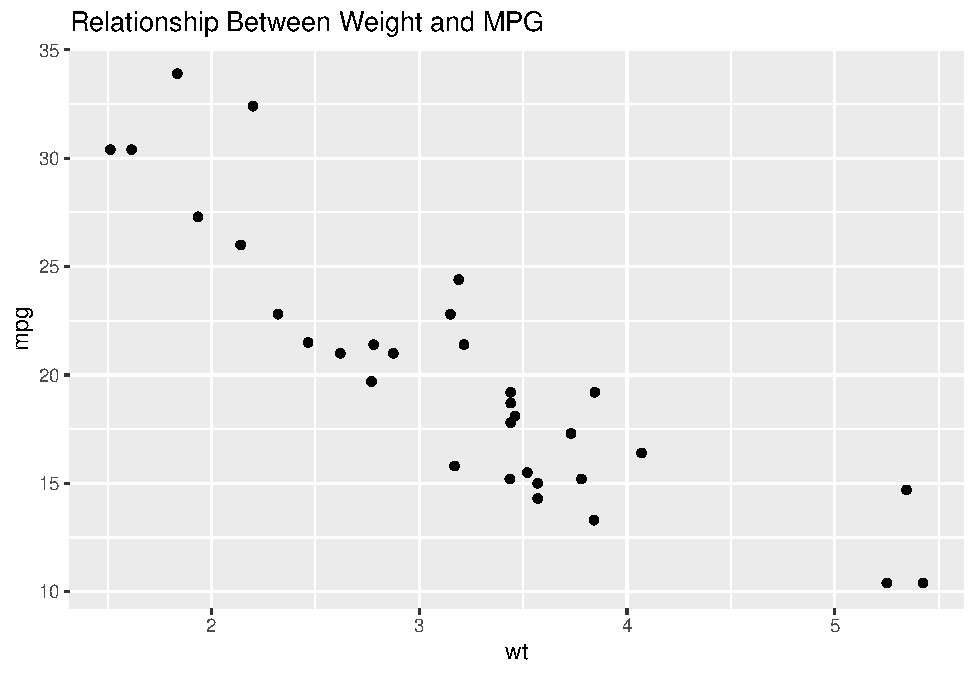
\includegraphics{psych-stats-book_files/figure-latex/unnamed-chunk-82-1.pdf}

\begin{Shaded}
\begin{Highlighting}[]
     \FunctionTok{ggsave}\NormalTok{(}\StringTok{"weight\_vs\_mpg.pdf"}\NormalTok{, }\AttributeTok{width =} \DecValTok{6}\NormalTok{, }\AttributeTok{height =} \DecValTok{4}\NormalTok{)}
\end{Highlighting}
\end{Shaded}

\begin{itemize}
\tightlist
\item
  This saves the plot as a PDF file, which can be opened in any PDF viewer or included in documents like research papers.
\end{itemize}

\begin{enumerate}
\def\labelenumi{\arabic{enumi}.}
\setcounter{enumi}{2}
\tightlist
\item
  \textbf{Customizing the Save Function}:

  \begin{itemize}
  \tightlist
  \item
    You can customize the save process further by specifying the device (e.g., PNG, PDF, JPEG) or by adjusting the size and resolution.
  \item
    Example: Saving as JPEG with custom dimensions
  \end{itemize}
\end{enumerate}

\begin{Shaded}
\begin{Highlighting}[]
     \FunctionTok{ggsave}\NormalTok{(}\StringTok{"weight\_vs\_mpg.jpg"}\NormalTok{, }\AttributeTok{width =} \DecValTok{8}\NormalTok{, }\AttributeTok{height =} \DecValTok{6}\NormalTok{, }\AttributeTok{dpi =} \DecValTok{300}\NormalTok{, }\AttributeTok{device =} \StringTok{"jpeg"}\NormalTok{)}
\end{Highlighting}
\end{Shaded}

\begin{itemize}
\tightlist
\item
  This saves the plot as a JPEG file with custom dimensions.
\end{itemize}

\begin{enumerate}
\def\labelenumi{\arabic{enumi}.}
\setcounter{enumi}{3}
\tightlist
\item
  \textbf{Saving Plots with Custom Names}:

  \begin{itemize}
  \tightlist
  \item
    You can also save plots with custom names that include variables or dynamic content.
  \item
    Example:
  \end{itemize}
\end{enumerate}

\begin{Shaded}
\begin{Highlighting}[]
\NormalTok{     plot\_name }\OtherTok{\textless{}{-}} \StringTok{"custom\_plot\_name"}
     \FunctionTok{ggsave}\NormalTok{(}\FunctionTok{paste0}\NormalTok{(plot\_name, }\StringTok{".png"}\NormalTok{), }\AttributeTok{width =} \DecValTok{6}\NormalTok{, }\AttributeTok{height =} \DecValTok{4}\NormalTok{, }\AttributeTok{dpi =} \DecValTok{300}\NormalTok{)}
\end{Highlighting}
\end{Shaded}

\begin{itemize}
\tightlist
\item
  This code saves the plot with a custom name stored in the \texttt{plot\_name} variable.
\end{itemize}

\begin{enumerate}
\def\labelenumi{\arabic{enumi}.}
\setcounter{enumi}{4}
\tightlist
\item
  \textbf{Saving Multiple Plots}:

  \begin{itemize}
  \tightlist
  \item
    If you have created multiple plots and want to save them all, you can assign each plot to a variable and use \texttt{ggsave()} on each.
  \item
    Example:
  \end{itemize}
\end{enumerate}

\begin{Shaded}
\begin{Highlighting}[]
\NormalTok{     plot1 }\OtherTok{\textless{}{-}} \FunctionTok{ggplot}\NormalTok{(mtcars, }\FunctionTok{aes}\NormalTok{(}\AttributeTok{x =}\NormalTok{ wt, }\AttributeTok{y =}\NormalTok{ mpg)) }\SpecialCharTok{+} \FunctionTok{geom\_point}\NormalTok{()}
\NormalTok{     plot2 }\OtherTok{\textless{}{-}} \FunctionTok{ggplot}\NormalTok{(mtcars, }\FunctionTok{aes}\NormalTok{(}\AttributeTok{x =}\NormalTok{ hp, }\AttributeTok{y =}\NormalTok{ mpg)) }\SpecialCharTok{+} \FunctionTok{geom\_point}\NormalTok{()}
     
     \FunctionTok{ggsave}\NormalTok{(}\StringTok{"plot1.png"}\NormalTok{, }\AttributeTok{plot =}\NormalTok{ plot1, }\AttributeTok{width =} \DecValTok{6}\NormalTok{, }\AttributeTok{height =} \DecValTok{4}\NormalTok{, }\AttributeTok{dpi =} \DecValTok{300}\NormalTok{)}
     \FunctionTok{ggsave}\NormalTok{(}\StringTok{"plot2.png"}\NormalTok{, }\AttributeTok{plot =}\NormalTok{ plot2, }\AttributeTok{width =} \DecValTok{6}\NormalTok{, }\AttributeTok{height =} \DecValTok{4}\NormalTok{, }\AttributeTok{dpi =} \DecValTok{300}\NormalTok{)}
\end{Highlighting}
\end{Shaded}

\begin{enumerate}
\def\labelenumi{\arabic{enumi}.}
\setcounter{enumi}{5}
\tightlist
\item
  \textbf{Exporting Plots from RStudio}:

  \begin{itemize}
  \tightlist
  \item
    In RStudio, you can also export plots directly from the Plot pane. After creating a plot:

    \begin{itemize}
    \tightlist
    \item
      Click the ``Export'' button above the plot.
    \item
      Choose ``Save as Image'' or ``Save as PDF'' and configure the file name, format, size, and resolution.
    \item
      Click ``Save'' to export the plot.
    \end{itemize}
  \end{itemize}
\item
  \textbf{Maintaining Plot Quality}:

  \begin{itemize}
  \tightlist
  \item
    When exporting plots, always ensure that the resolution (dpi) is high enough for your intended use. For web or presentation use, 72-150 dpi may be sufficient. For print or publication, 300 dpi is the standard.
  \end{itemize}
\end{enumerate}

By mastering these steps, you'll be able to save and share your ggplot2 visualizations in various formats, ensuring they maintain their quality and clarity for any audience.

\hypertarget{introduction-to-apa-formatting}{%
\section{Introduction to APA Formatting}\label{introduction-to-apa-formatting}}

In psychological research, clear and consistent communication of data is crucial. The American Psychological Association (APA) has established a set of guidelines for formatting research papers, including how to present graphs and figures. Adhering to these standards ensures that your research is presented professionally and is easily understood by others in the field.

\hypertarget{what-is-apa-formatting}{%
\subsection{What is APA Formatting?}\label{what-is-apa-formatting}}

\textbf{APA Formatting} refers to the standardized style guidelines established by the American Psychological Association, which are widely used in psychology and other social sciences. These guidelines cover everything from how to structure a research paper to how to format citations, tables, and figures, including graphs.

\textbf{Overview of APA Style Guidelines for Graphing}:\\
- \textbf{Consistency}: APA style promotes consistency across all elements of a research paper, including graphs. This ensures that all figures are presented in a uniform manner, making it easier for readers to interpret the data.\\
- \textbf{Clarity}: APA emphasizes clarity in data presentation, meaning that graphs should be easy to read and understand. This involves careful selection of graph types, appropriate scaling, and clear labeling.\\
- \textbf{Precision}: APA guidelines encourage precise presentation of data, ensuring that graphs accurately represent the underlying data without distortion or exaggeration.\\
- \textbf{Professionalism}: Adhering to APA standards helps present your research in a professional manner, which is particularly important for publication in academic journals and presentations at conferences.

\textbf{Importance of Adhering to APA Standards in Psychological Research}:\\
- \textbf{Credibility}: Following APA guidelines enhances the credibility of your research by demonstrating attention to detail and a commitment to professional standards.\\
- \textbf{Ease of Communication}: APA-compliant graphs are easier for other researchers to understand and interpret, facilitating better communication of your findings.\\
- \textbf{Publication Requirements}: Most psychology journals require submissions to adhere to APA style, including the formatting of graphs and figures. Ensuring that your graphs meet these standards can streamline the publication process.

\hypertarget{key-elements-of-apa-formatted-graphs}{%
\subsection{Key Elements of APA-Formatted Graphs}\label{key-elements-of-apa-formatted-graphs}}

When formatting graphs according to APA style, there are several key elements to consider:

\begin{enumerate}
\def\labelenumi{\arabic{enumi}.}
\tightlist
\item
  \textbf{Titles and Axis Labels}:

  \begin{itemize}
  \tightlist
  \item
    \textbf{Title}: Every graph should have a clear, descriptive title that concisely conveys what the graph is about. The title should be placed above the graph, not on it.
  \item
    \textbf{Axis Labels}: Both the x-axis and y-axis must be labeled with the name of the variable and the units of measurement, if applicable. Axis labels should be straightforward and easily understood.
  \end{itemize}
\item
  \textbf{Legends}:

  \begin{itemize}
  \tightlist
  \item
    \textbf{Placement}: Legends should be placed within the plot area, often in a corner where they do not obscure the data. If possible, position the legend outside the plot area for a cleaner appearance.
  \item
    \textbf{Content}: Legends should clearly explain any colors, shapes, or lines used in the graph. For example, if different colors represent different groups, the legend should indicate which color corresponds to each group.
  \end{itemize}
\item
  \textbf{Font Size and Style}:

  \begin{itemize}
  \tightlist
  \item
    \textbf{Font Size}: APA guidelines recommend using a font size that is readable when the graph is printed at the final size. Typically, 10 to 12-point font is appropriate for axis labels and titles.
  \item
    \textbf{Font Style}: Use a sans-serif font like Arial or Helvetica for readability. Ensure that all text is clear and consistent throughout the graph.
  \end{itemize}
\item
  \textbf{Line Thickness}:

  \begin{itemize}
  \tightlist
  \item
    \textbf{Lines}: APA recommends using a consistent line thickness that is neither too thick nor too thin. Lines should be easily distinguishable but not overpowering.
  \item
    \textbf{Error Bars}: If your graph includes error bars, they should be clearly visible and easy to interpret, typically using a medium line thickness.
  \end{itemize}
\item
  \textbf{Color and Contrast}:

  \begin{itemize}
  \tightlist
  \item
    \textbf{Colors}: Use colors that are distinct and provide sufficient contrast. Avoid using too many colors, and ensure that all colors are distinguishable, even for those with color vision deficiencies.
  \item
    \textbf{Greyscale}: If your graph will be printed in black and white, ensure that different elements are still distinguishable by using varying shades of grey or different line types (e.g., solid, dashed).
  \end{itemize}
\item
  \textbf{Grid Lines}:

  \begin{itemize}
  \tightlist
  \item
    \textbf{Visibility}: Grid lines should be kept to a minimum and should not detract from the data. APA guidelines suggest using light grey grid lines or none at all, depending on the graph.
  \item
    \textbf{Placement}: If grid lines are used, they should be subtle and only included where necessary to aid in interpreting the data.
  \end{itemize}
\end{enumerate}

\hypertarget{example-comparing-a-standard-ggplot2-graph-with-an-apa-compliant-graph}{%
\subsection{Example: Comparing a Standard ggplot2 Graph with an APA-Compliant Graph}\label{example-comparing-a-standard-ggplot2-graph-with-an-apa-compliant-graph}}

Let's compare a basic ggplot2 graph with an APA-compliant version to highlight the key differences.

\textbf{Standard ggplot2 Graph}:

\begin{Shaded}
\begin{Highlighting}[]
\FunctionTok{library}\NormalTok{(ggplot2)}

\CommentTok{\# Basic scatter plot}
\FunctionTok{ggplot}\NormalTok{(mtcars, }\FunctionTok{aes}\NormalTok{(}\AttributeTok{x =}\NormalTok{ wt, }\AttributeTok{y =}\NormalTok{ mpg)) }\SpecialCharTok{+}
  \FunctionTok{geom\_point}\NormalTok{() }\SpecialCharTok{+}
  \FunctionTok{labs}\NormalTok{(}\AttributeTok{title =} \StringTok{"Scatter Plot of Weight vs. MPG"}\NormalTok{,}
       \AttributeTok{x =} \StringTok{"Weight (1000 lbs)"}\NormalTok{,}
       \AttributeTok{y =} \StringTok{"Miles Per Gallon"}\NormalTok{)}
\end{Highlighting}
\end{Shaded}

\includegraphics{psych-stats-book_files/figure-latex/unnamed-chunk-86-1.pdf}

This graph includes a title, axis labels, and points representing data. However, it doesn't fully adhere to APA formatting guidelines.

\textbf{APA-Compliant Graph}:

\begin{Shaded}
\begin{Highlighting}[]
\FunctionTok{ggplot}\NormalTok{(mtcars, }\FunctionTok{aes}\NormalTok{(}\AttributeTok{x =}\NormalTok{ wt, }\AttributeTok{y =}\NormalTok{ mpg)) }\SpecialCharTok{+}
  \FunctionTok{geom\_point}\NormalTok{(}\AttributeTok{size =} \DecValTok{3}\NormalTok{, }\AttributeTok{color =} \StringTok{"black"}\NormalTok{) }\SpecialCharTok{+}  \CommentTok{\# Black points for better contrast}
  \FunctionTok{geom\_smooth}\NormalTok{(}\AttributeTok{method =} \StringTok{"lm"}\NormalTok{, }\AttributeTok{se =} \ConstantTok{FALSE}\NormalTok{, }\AttributeTok{color =} \StringTok{"black"}\NormalTok{, }\AttributeTok{linetype =} \StringTok{"dashed"}\NormalTok{) }\SpecialCharTok{+}  \CommentTok{\# Adding a trend line}
  \FunctionTok{labs}\NormalTok{(}\AttributeTok{title =} \StringTok{"Relationship Between Car Weight and Fuel Efficiency"}\NormalTok{,}
       \AttributeTok{x =} \StringTok{"Car Weight (in 1000 lbs)"}\NormalTok{,}
       \AttributeTok{y =} \StringTok{"Fuel Efficiency (MPG)"}\NormalTok{) }\SpecialCharTok{+}
  \FunctionTok{theme\_minimal}\NormalTok{() }\SpecialCharTok{+}  \CommentTok{\# Apply a clean theme}
  \FunctionTok{theme}\NormalTok{(}\AttributeTok{plot.title =} \FunctionTok{element\_text}\NormalTok{(}\AttributeTok{hjust =} \FloatTok{0.5}\NormalTok{, }\AttributeTok{size =} \DecValTok{14}\NormalTok{, }\AttributeTok{face =} \StringTok{"bold"}\NormalTok{),}
        \AttributeTok{axis.title =} \FunctionTok{element\_text}\NormalTok{(}\AttributeTok{size =} \DecValTok{12}\NormalTok{),}
        \AttributeTok{axis.text =} \FunctionTok{element\_text}\NormalTok{(}\AttributeTok{size =} \DecValTok{10}\NormalTok{),}
        \AttributeTok{legend.position =} \StringTok{"none"}\NormalTok{)  }\CommentTok{\# Removing legend for simplicity}
\end{Highlighting}
\end{Shaded}

\begin{verbatim}
## `geom_smooth()` using formula = 'y ~ x'
\end{verbatim}

\includegraphics{psych-stats-book_files/figure-latex/unnamed-chunk-87-1.pdf}

\textbf{Key Changes in the APA-Compliant Graph}:\\
- \textbf{Title}: The title is more descriptive and centered above the graph.\\
- \textbf{Axis Labels}: The axis labels are slightly larger and more descriptive, including units of measurement.\\
- \textbf{Font Size and Style}: The font size is adjusted for readability, and a sans-serif font is used.\\
- \textbf{Color and Line Thickness}: The points are black for better contrast, and a dashed line is added to represent the trend, which is typical in APA formatting.\\
- \textbf{Legend}: The legend is removed in this example, as it's unnecessary for a single variable plot, reducing clutter.

By following these guidelines, your graphs will not only meet APA standards but also effectively communicate your data, making your research more accessible and impactful.

\hypertarget{creating-apa-formatted-graphs-with-ggplot2}{%
\section{Creating APA-Formatted Graphs with ggplot2}\label{creating-apa-formatted-graphs-with-ggplot2}}

Creating graphs that adhere to APA formatting guidelines in ggplot2 involves a series of modifications to the default plots. This section will guide you through the process of adjusting your ggplot2 plots to meet APA standards, customizing themes for compliance, and creating common APA-formatted graphs. We'll also cover how to add annotations and legends that align with APA guidelines.

\hypertarget{modifying-ggplot2-plots-to-meet-apa-standards}{%
\subsection{Modifying ggplot2 Plots to Meet APA Standards}\label{modifying-ggplot2-plots-to-meet-apa-standards}}

To modify a ggplot2 plot to meet APA standards, you'll need to adjust various elements such as font sizes, line thickness, and overall layout. Below is a step-by-step guide on how to do this.

\begin{enumerate}
\def\labelenumi{\arabic{enumi}.}
\tightlist
\item
  \textbf{Adjusting Font Sizes}:

  \begin{itemize}
  \tightlist
  \item
    APA guidelines recommend using a legible font size for titles, axis labels, and text. Typically, you'll want to use a font size of around 10-12 points for axis labels and slightly larger for titles.
  \item
    Example:
  \end{itemize}
\end{enumerate}

\begin{Shaded}
\begin{Highlighting}[]
     \FunctionTok{ggplot}\NormalTok{(mtcars, }\FunctionTok{aes}\NormalTok{(}\AttributeTok{x =}\NormalTok{ wt, }\AttributeTok{y =}\NormalTok{ mpg)) }\SpecialCharTok{+}
       \FunctionTok{geom\_point}\NormalTok{(}\AttributeTok{size =} \DecValTok{3}\NormalTok{) }\SpecialCharTok{+}
       \FunctionTok{labs}\NormalTok{(}\AttributeTok{title =} \StringTok{"Relationship Between Car Weight and MPG"}\NormalTok{,}
            \AttributeTok{x =} \StringTok{"Car Weight (in 1000 lbs)"}\NormalTok{,}
            \AttributeTok{y =} \StringTok{"Miles Per Gallon"}\NormalTok{) }\SpecialCharTok{+}
       \FunctionTok{theme\_minimal}\NormalTok{() }\SpecialCharTok{+}
       \FunctionTok{theme}\NormalTok{(}
         \AttributeTok{plot.title =} \FunctionTok{element\_text}\NormalTok{(}\AttributeTok{size =} \DecValTok{14}\NormalTok{, }\AttributeTok{face =} \StringTok{"bold"}\NormalTok{),}
         \AttributeTok{axis.title =} \FunctionTok{element\_text}\NormalTok{(}\AttributeTok{size =} \DecValTok{12}\NormalTok{),}
         \AttributeTok{axis.text =} \FunctionTok{element\_text}\NormalTok{(}\AttributeTok{size =} \DecValTok{10}\NormalTok{)}
\NormalTok{       )}
\end{Highlighting}
\end{Shaded}

\includegraphics{psych-stats-book_files/figure-latex/unnamed-chunk-88-1.pdf}

\begin{enumerate}
\def\labelenumi{\arabic{enumi}.}
\setcounter{enumi}{1}
\tightlist
\item
  \textbf{Modifying Line Thickness}:

  \begin{itemize}
  \tightlist
  \item
    Line thickness should be consistent and not too heavy or light. APA guidelines generally prefer moderate line thickness for clarity.
  \item
    Example:
  \end{itemize}
\end{enumerate}

\begin{Shaded}
\begin{Highlighting}[]
     \FunctionTok{ggplot}\NormalTok{(mtcars, }\FunctionTok{aes}\NormalTok{(}\AttributeTok{x =}\NormalTok{ wt, }\AttributeTok{y =}\NormalTok{ mpg)) }\SpecialCharTok{+}
       \FunctionTok{geom\_point}\NormalTok{(}\AttributeTok{size =} \DecValTok{3}\NormalTok{) }\SpecialCharTok{+}
       \FunctionTok{geom\_smooth}\NormalTok{(}\AttributeTok{method =} \StringTok{"lm"}\NormalTok{, }\AttributeTok{se =} \ConstantTok{FALSE}\NormalTok{, }\AttributeTok{color =} \StringTok{"black"}\NormalTok{, }\AttributeTok{linetype =} \StringTok{"solid"}\NormalTok{, }\AttributeTok{size =} \FloatTok{0.7}\NormalTok{) }\SpecialCharTok{+}
       \FunctionTok{labs}\NormalTok{(}\AttributeTok{title =} \StringTok{"Relationship Between Car Weight and MPG"}\NormalTok{,}
            \AttributeTok{x =} \StringTok{"Car Weight (in 1000 lbs)"}\NormalTok{,}
            \AttributeTok{y =} \StringTok{"Miles Per Gallon"}\NormalTok{) }\SpecialCharTok{+}
       \FunctionTok{theme\_minimal}\NormalTok{() }\SpecialCharTok{+}
        \FunctionTok{theme}\NormalTok{(}
    \AttributeTok{plot.title =} \FunctionTok{element\_text}\NormalTok{(}\AttributeTok{size =} \DecValTok{14}\NormalTok{, }\AttributeTok{face =} \StringTok{"bold"}\NormalTok{),}
    \AttributeTok{axis.title =} \FunctionTok{element\_text}\NormalTok{(}\AttributeTok{size =} \DecValTok{12}\NormalTok{),}
    \AttributeTok{axis.text =} \FunctionTok{element\_text}\NormalTok{(}\AttributeTok{size =} \DecValTok{10}\NormalTok{),}
    \AttributeTok{panel.grid.major =} \FunctionTok{element\_blank}\NormalTok{(),  }\CommentTok{\# Remove major grid lines}
    \AttributeTok{panel.grid.minor =} \FunctionTok{element\_blank}\NormalTok{(),  }\CommentTok{\# Remove minor grid lines}
    \AttributeTok{panel.border =} \FunctionTok{element\_rect}\NormalTok{(}\AttributeTok{color =} \StringTok{"black"}\NormalTok{, }\AttributeTok{size =} \FloatTok{0.5}\NormalTok{, }\AttributeTok{fill =} \ConstantTok{NA}\NormalTok{)  }\CommentTok{\# Ensure the panel background is not filled}
\NormalTok{  )}
\end{Highlighting}
\end{Shaded}

\includegraphics{psych-stats-book_files/figure-latex/unnamed-chunk-89-1.pdf}

\begin{enumerate}
\def\labelenumi{\arabic{enumi}.}
\setcounter{enumi}{2}
\tightlist
\item
  \textbf{Other Formatting Details}:

  \begin{itemize}
  \tightlist
  \item
    Additional APA adjustments include removing unnecessary grid lines, ensuring that legends are placed appropriately, and making sure that colors provide sufficient contrast.
  \end{itemize}
\end{enumerate}

\begin{Shaded}
\begin{Highlighting}[]
     \FunctionTok{ggplot}\NormalTok{(mtcars, }\FunctionTok{aes}\NormalTok{(}\AttributeTok{x =}\NormalTok{ wt, }\AttributeTok{y =}\NormalTok{ mpg)) }\SpecialCharTok{+}
       \FunctionTok{geom\_point}\NormalTok{(}\AttributeTok{size =} \DecValTok{3}\NormalTok{, }\AttributeTok{color =} \StringTok{"black"}\NormalTok{) }\SpecialCharTok{+}
       \FunctionTok{geom\_smooth}\NormalTok{(}\AttributeTok{method =} \StringTok{"lm"}\NormalTok{, }\AttributeTok{se =} \ConstantTok{FALSE}\NormalTok{, }\AttributeTok{color =} \StringTok{"black"}\NormalTok{, }\AttributeTok{linetype =} \StringTok{"dashed"}\NormalTok{, }\AttributeTok{size =} \FloatTok{0.7}\NormalTok{) }\SpecialCharTok{+}
       \FunctionTok{labs}\NormalTok{(}\AttributeTok{title =} \StringTok{"Relationship Between Car Weight and MPG"}\NormalTok{,}
            \AttributeTok{x =} \StringTok{"Car Weight (in 1000 lbs)"}\NormalTok{,}
            \AttributeTok{y =} \StringTok{"Miles Per Gallon"}\NormalTok{) }\SpecialCharTok{+}
       \FunctionTok{theme\_minimal}\NormalTok{() }\SpecialCharTok{+}
       \FunctionTok{theme}\NormalTok{(}
         \AttributeTok{plot.title =} \FunctionTok{element\_text}\NormalTok{(}\AttributeTok{size =} \DecValTok{14}\NormalTok{, }\AttributeTok{face =} \StringTok{"bold"}\NormalTok{),}
         \AttributeTok{axis.title =} \FunctionTok{element\_text}\NormalTok{(}\AttributeTok{size =} \DecValTok{12}\NormalTok{),}
         \AttributeTok{axis.text =} \FunctionTok{element\_text}\NormalTok{(}\AttributeTok{size =} \DecValTok{10}\NormalTok{),}
         \AttributeTok{panel.grid.major =} \FunctionTok{element\_blank}\NormalTok{(),  }\CommentTok{\# Remove major grid lines}
    \AttributeTok{panel.grid.minor =} \FunctionTok{element\_blank}\NormalTok{(),  }\CommentTok{\# Remove minor grid lines}
    \AttributeTok{panel.border =} \FunctionTok{element\_rect}\NormalTok{(}\AttributeTok{color =} \StringTok{"black"}\NormalTok{, }\AttributeTok{size =} \FloatTok{0.5}\NormalTok{, }\AttributeTok{fill =} \ConstantTok{NA}\NormalTok{),  }\CommentTok{\# Ensure the panel background is not filled}
         \AttributeTok{legend.position =} \StringTok{"top"}
\NormalTok{       )}
\end{Highlighting}
\end{Shaded}

\includegraphics{psych-stats-book_files/figure-latex/unnamed-chunk-90-1.pdf}

\hypertarget{using-theme-options-for-apa-compliance}{%
\subsection{Using Theme Options for APA Compliance}\label{using-theme-options-for-apa-compliance}}

To streamline the process of creating APA-compliant graphs, ggplot2 offers theme options that can be customized to fit APA guidelines. By modifying these themes, you can ensure that your graphs meet APA standards consistently.

\begin{enumerate}
\def\labelenumi{\arabic{enumi}.}
\tightlist
\item
  \textbf{Customizing the Theme}:

  \begin{itemize}
  \tightlist
  \item
    The \texttt{theme()} function in ggplot2 allows you to customize various elements of your plot, including text size, font style, grid lines, and panel borders.
  \item
    Example:
  \end{itemize}
\end{enumerate}

\begin{Shaded}
\begin{Highlighting}[]
\NormalTok{     custom\_theme }\OtherTok{\textless{}{-}} \FunctionTok{theme}\NormalTok{(}
       \AttributeTok{plot.title =} \FunctionTok{element\_text}\NormalTok{(}\AttributeTok{hjust =} \FloatTok{0.5}\NormalTok{, }\AttributeTok{size =} \DecValTok{14}\NormalTok{, }\AttributeTok{face =} \StringTok{"bold"}\NormalTok{),}
       \AttributeTok{axis.title =} \FunctionTok{element\_text}\NormalTok{(}\AttributeTok{size =} \DecValTok{12}\NormalTok{),}
       \AttributeTok{axis.text =} \FunctionTok{element\_text}\NormalTok{(}\AttributeTok{size =} \DecValTok{10}\NormalTok{),}
       \AttributeTok{legend.position =} \StringTok{"top"}\NormalTok{,}
       \AttributeTok{panel.grid.major =} \FunctionTok{element\_blank}\NormalTok{(),  }\CommentTok{\# Remove major grid lines}
    \AttributeTok{panel.grid.minor =} \FunctionTok{element\_blank}\NormalTok{(),  }\CommentTok{\# Remove minor grid lines}
    \AttributeTok{panel.border =} \FunctionTok{element\_rect}\NormalTok{(}\AttributeTok{color =} \StringTok{"black"}\NormalTok{, }\AttributeTok{size =} \FloatTok{0.5}\NormalTok{, }\AttributeTok{fill =} \ConstantTok{NA}\NormalTok{)  }\CommentTok{\# Ensure the panel background is not filled}
\NormalTok{     )}

     \FunctionTok{ggplot}\NormalTok{(mtcars, }\FunctionTok{aes}\NormalTok{(}\AttributeTok{x =}\NormalTok{ wt, }\AttributeTok{y =}\NormalTok{ mpg)) }\SpecialCharTok{+}
       \FunctionTok{geom\_point}\NormalTok{(}\AttributeTok{size =} \DecValTok{3}\NormalTok{, }\AttributeTok{color =} \StringTok{"black"}\NormalTok{) }\SpecialCharTok{+}
       \FunctionTok{geom\_smooth}\NormalTok{(}\AttributeTok{method =} \StringTok{"lm"}\NormalTok{, }\AttributeTok{se =} \ConstantTok{FALSE}\NormalTok{, }\AttributeTok{color =} \StringTok{"black"}\NormalTok{, }\AttributeTok{linetype =} \StringTok{"dashed"}\NormalTok{, }\AttributeTok{size =} \FloatTok{0.7}\NormalTok{) }\SpecialCharTok{+}
       \FunctionTok{labs}\NormalTok{(}\AttributeTok{title =} \StringTok{"Relationship Between Car Weight and MPG"}\NormalTok{,}
            \AttributeTok{x =} \StringTok{"Car Weight (in 1000 lbs)"}\NormalTok{,}
            \AttributeTok{y =} \StringTok{"Miles Per Gallon"}\NormalTok{) }\SpecialCharTok{+}
\NormalTok{       custom\_theme}
\end{Highlighting}
\end{Shaded}

\begin{verbatim}
## `geom_smooth()` using formula = 'y ~ x'
\end{verbatim}

\includegraphics{psych-stats-book_files/figure-latex/unnamed-chunk-91-1.pdf}

\begin{enumerate}
\def\labelenumi{\arabic{enumi}.}
\setcounter{enumi}{1}
\tightlist
\item
  \textbf{Example: Applying the Custom Theme for APA Compliance}:

  \begin{itemize}
  \tightlist
  \item
    The example above creates a custom theme that can be reused across multiple plots to ensure consistency with APA formatting.
  \item
    This theme sets the font size and style for titles, axis labels, and axis text, removes unnecessary grid lines, and adjusts the legend position and panel borders.
  \end{itemize}
\end{enumerate}

\hypertarget{common-apa-formatted-graphs}{%
\subsection{Common APA-Formatted Graphs}\label{common-apa-formatted-graphs}}

Creating different types of graphs that adhere to APA formatting requires specific adjustments based on the graph type. Below are examples for bar graphs, line graphs, scatter plots, and box plots.

\begin{enumerate}
\def\labelenumi{\arabic{enumi}.}
\tightlist
\item
  \textbf{Bar Graphs}:

  \begin{itemize}
  \tightlist
  \item
    Bar graphs are commonly used in APA-style research to compare categories or groups. Error bars are often included to represent variability.
  \item
    Example:
  \end{itemize}
\end{enumerate}

\begin{Shaded}
\begin{Highlighting}[]
     \FunctionTok{ggplot}\NormalTok{(mtcars, }\FunctionTok{aes}\NormalTok{(}\AttributeTok{x =} \FunctionTok{factor}\NormalTok{(cyl), }\AttributeTok{y =}\NormalTok{ mpg)) }\SpecialCharTok{+}
       \FunctionTok{geom\_bar}\NormalTok{(}\AttributeTok{stat =} \StringTok{"summary"}\NormalTok{, }\AttributeTok{fun =} \StringTok{"mean"}\NormalTok{, }\AttributeTok{fill =} \StringTok{"lightblue"}\NormalTok{, }\AttributeTok{color =} \StringTok{"black"}\NormalTok{) }\SpecialCharTok{+}
       \FunctionTok{geom\_errorbar}\NormalTok{(}\AttributeTok{stat =} \StringTok{"summary"}\NormalTok{, }\AttributeTok{fun.data =} \StringTok{"mean\_se"}\NormalTok{, }\AttributeTok{width =} \FloatTok{0.2}\NormalTok{) }\SpecialCharTok{+}
       \FunctionTok{labs}\NormalTok{(}\AttributeTok{title =} \StringTok{"Average MPG by Cylinder Count"}\NormalTok{,}
            \AttributeTok{x =} \StringTok{"Number of Cylinders"}\NormalTok{,}
            \AttributeTok{y =} \StringTok{"Miles Per Gallon"}\NormalTok{) }\SpecialCharTok{+}
\NormalTok{       custom\_theme}
\end{Highlighting}
\end{Shaded}

\includegraphics{psych-stats-book_files/figure-latex/unnamed-chunk-92-1.pdf}

\begin{enumerate}
\def\labelenumi{\arabic{enumi}.}
\setcounter{enumi}{1}
\tightlist
\item
  \textbf{Line Graphs}:

  \begin{itemize}
  \tightlist
  \item
    Line graphs are used to show trends over time or across conditions. When multiple groups are involved, different line types or colors are used.
  \item
    Example:
  \end{itemize}
\end{enumerate}

\begin{Shaded}
\begin{Highlighting}[]
     \FunctionTok{ggplot}\NormalTok{(mtcars, }\FunctionTok{aes}\NormalTok{(}\AttributeTok{x =}\NormalTok{ wt, }\AttributeTok{y =}\NormalTok{ mpg, }\AttributeTok{color =} \FunctionTok{factor}\NormalTok{(cyl))) }\SpecialCharTok{+}
       \FunctionTok{geom\_line}\NormalTok{() }\SpecialCharTok{+}
       \FunctionTok{labs}\NormalTok{(}\AttributeTok{title =} \StringTok{"MPG vs. Weight by Cylinder Count"}\NormalTok{,}
            \AttributeTok{x =} \StringTok{"Weight (1000 lbs)"}\NormalTok{,}
            \AttributeTok{y =} \StringTok{"Miles Per Gallon"}\NormalTok{,}
            \AttributeTok{color =} \StringTok{"Cylinders"}\NormalTok{) }\SpecialCharTok{+}
\NormalTok{       custom\_theme}
\end{Highlighting}
\end{Shaded}

\includegraphics{psych-stats-book_files/figure-latex/unnamed-chunk-93-1.pdf}

\begin{enumerate}
\def\labelenumi{\arabic{enumi}.}
\setcounter{enumi}{2}
\tightlist
\item
  \textbf{Scatter Plots}:

  \begin{itemize}
  \tightlist
  \item
    Scatter plots display relationships between two continuous variables. Trend lines (such as linear regression lines) are often added in APA-compliant scatter plots.
  \item
    Example:
  \end{itemize}
\end{enumerate}

\begin{Shaded}
\begin{Highlighting}[]
     \FunctionTok{ggplot}\NormalTok{(mtcars, }\FunctionTok{aes}\NormalTok{(}\AttributeTok{x =}\NormalTok{ wt, }\AttributeTok{y =}\NormalTok{ mpg)) }\SpecialCharTok{+}
       \FunctionTok{geom\_point}\NormalTok{(}\AttributeTok{size =} \DecValTok{3}\NormalTok{, }\AttributeTok{color =} \StringTok{"black"}\NormalTok{) }\SpecialCharTok{+}
       \FunctionTok{geom\_smooth}\NormalTok{(}\AttributeTok{method =} \StringTok{"lm"}\NormalTok{, }\AttributeTok{se =} \ConstantTok{FALSE}\NormalTok{, }\AttributeTok{color =} \StringTok{"black"}\NormalTok{, }\AttributeTok{linetype =} \StringTok{"dashed"}\NormalTok{, }\AttributeTok{size =} \FloatTok{0.7}\NormalTok{) }\SpecialCharTok{+}
       \FunctionTok{labs}\NormalTok{(}\AttributeTok{title =} \StringTok{"Scatter Plot of Weight and MPG"}\NormalTok{,}
            \AttributeTok{x =} \StringTok{"Weight (1000 lbs)"}\NormalTok{,}
            \AttributeTok{y =} \StringTok{"Miles Per Gallon"}\NormalTok{) }\SpecialCharTok{+}
\NormalTok{       custom\_theme}
\end{Highlighting}
\end{Shaded}

\begin{verbatim}
## `geom_smooth()` using formula = 'y ~ x'
\end{verbatim}

\includegraphics{psych-stats-book_files/figure-latex/unnamed-chunk-94-1.pdf}

\begin{enumerate}
\def\labelenumi{\arabic{enumi}.}
\setcounter{enumi}{3}
\tightlist
\item
  \textbf{Box Plots}:

  \begin{itemize}
  \tightlist
  \item
    Box plots are used to summarize the distribution of a dataset by displaying the median, quartiles, and potential outliers.
  \item
    Example:
  \end{itemize}
\end{enumerate}

\begin{Shaded}
\begin{Highlighting}[]
     \FunctionTok{ggplot}\NormalTok{(mtcars, }\FunctionTok{aes}\NormalTok{(}\AttributeTok{x =} \FunctionTok{factor}\NormalTok{(cyl), }\AttributeTok{y =}\NormalTok{ mpg)) }\SpecialCharTok{+}
       \FunctionTok{geom\_boxplot}\NormalTok{(}\AttributeTok{fill =} \StringTok{"lightblue"}\NormalTok{, }\AttributeTok{color =} \StringTok{"black"}\NormalTok{) }\SpecialCharTok{+}
       \FunctionTok{labs}\NormalTok{(}\AttributeTok{title =} \StringTok{"Distribution of MPG by Cylinder Count"}\NormalTok{,}
            \AttributeTok{x =} \StringTok{"Number of Cylinders"}\NormalTok{,}
            \AttributeTok{y =} \StringTok{"Miles Per Gallon"}\NormalTok{) }\SpecialCharTok{+}
\NormalTok{       custom\_theme}
\end{Highlighting}
\end{Shaded}

\includegraphics{psych-stats-book_files/figure-latex/unnamed-chunk-95-1.pdf}

\hypertarget{adding-annotations-and-apa-legends}{%
\subsection{Adding Annotations and APA Legends}\label{adding-annotations-and-apa-legends}}

Annotations and legends are essential for providing additional context and clarity in APA-compliant graphs.

\begin{enumerate}
\def\labelenumi{\arabic{enumi}.}
\tightlist
\item
  \textbf{Adding APA-Compliant Annotations}:

  \begin{itemize}
  \tightlist
  \item
    Annotations can be added to highlight specific data points or trends in the graph. In APA formatting, these annotations should be clear and unobtrusive.
  \item
    Example:
  \end{itemize}
\end{enumerate}

\begin{Shaded}
\begin{Highlighting}[]
     \FunctionTok{ggplot}\NormalTok{(mtcars, }\FunctionTok{aes}\NormalTok{(}\AttributeTok{x =}\NormalTok{ wt, }\AttributeTok{y =}\NormalTok{ mpg)) }\SpecialCharTok{+}
       \FunctionTok{geom\_point}\NormalTok{(}\AttributeTok{size =} \DecValTok{3}\NormalTok{, }\AttributeTok{color =} \StringTok{"black"}\NormalTok{) }\SpecialCharTok{+}
       \FunctionTok{geom\_smooth}\NormalTok{(}\AttributeTok{method =} \StringTok{"lm"}\NormalTok{, }\AttributeTok{se =} \ConstantTok{FALSE}\NormalTok{, }\AttributeTok{color =} \StringTok{"black"}\NormalTok{, }\AttributeTok{linetype =} \StringTok{"dashed"}\NormalTok{, }\AttributeTok{size =} \FloatTok{0.7}\NormalTok{) }\SpecialCharTok{+}
       \FunctionTok{annotate}\NormalTok{(}\StringTok{"text"}\NormalTok{, }\AttributeTok{x =} \FloatTok{4.5}\NormalTok{, }\AttributeTok{y =} \DecValTok{25}\NormalTok{, }\AttributeTok{label =} \StringTok{"Trend Line"}\NormalTok{, }\AttributeTok{hjust =} \DecValTok{0}\NormalTok{, }\AttributeTok{size =} \DecValTok{4}\NormalTok{, }\AttributeTok{color =} \StringTok{"black"}\NormalTok{) }\SpecialCharTok{+}
       \FunctionTok{labs}\NormalTok{(}\AttributeTok{title =} \StringTok{"Scatter Plot of Weight and MPG"}\NormalTok{,}
            \AttributeTok{x =} \StringTok{"Weight (1000 lbs)"}\NormalTok{,}
            \AttributeTok{y =} \StringTok{"Miles Per Gallon"}\NormalTok{) }\SpecialCharTok{+}
\NormalTok{       custom\_theme}
\end{Highlighting}
\end{Shaded}

\begin{verbatim}
## `geom_smooth()` using formula = 'y ~ x'
\end{verbatim}

\includegraphics{psych-stats-book_files/figure-latex/unnamed-chunk-96-1.pdf}

\begin{enumerate}
\def\labelenumi{\arabic{enumi}.}
\setcounter{enumi}{1}
\tightlist
\item
  \textbf{Positioning the Legend According to APA Guidelines}:

  \begin{itemize}
  \tightlist
  \item
    APA guidelines suggest placing legends outside the plot area to avoid cluttering the graph. The legend should be easily readable and positioned to enhance the graph's clarity.
  \item
    Example:
  \end{itemize}
\end{enumerate}

\begin{Shaded}
\begin{Highlighting}[]
     \FunctionTok{ggplot}\NormalTok{(mtcars, }\FunctionTok{aes}\NormalTok{(}\AttributeTok{x =}\NormalTok{ wt, }\AttributeTok{y =}\NormalTok{ mpg, }\AttributeTok{color =} \FunctionTok{factor}\NormalTok{(cyl))) }\SpecialCharTok{+}
       \FunctionTok{geom\_point}\NormalTok{(}\AttributeTok{size =} \DecValTok{3}\NormalTok{) }\SpecialCharTok{+}
       \FunctionTok{geom\_smooth}\NormalTok{(}\AttributeTok{method =} \StringTok{"lm}

\StringTok{"}\NormalTok{, }\AttributeTok{se =} \ConstantTok{FALSE}\NormalTok{, }\AttributeTok{linetype =} \StringTok{"dashed"}\NormalTok{, }\AttributeTok{size =} \FloatTok{0.7}\NormalTok{) }\SpecialCharTok{+}
       \FunctionTok{labs}\NormalTok{(}\AttributeTok{title =} \StringTok{"MPG vs. Weight by Cylinder Count"}\NormalTok{,}
            \AttributeTok{x =} \StringTok{"Weight (1000 lbs)"}\NormalTok{,}
            \AttributeTok{y =} \StringTok{"Miles Per Gallon"}\NormalTok{,}
            \AttributeTok{color =} \StringTok{"Cylinders"}\NormalTok{) }\SpecialCharTok{+}
\NormalTok{       custom\_theme }\SpecialCharTok{+}
       \FunctionTok{theme}\NormalTok{(}
         \AttributeTok{legend.position =} \StringTok{"right"}\NormalTok{,  }\CommentTok{\# Position the legend to the right of the plot}
         \AttributeTok{legend.title =} \FunctionTok{element\_text}\NormalTok{(}\AttributeTok{size =} \DecValTok{12}\NormalTok{, }\AttributeTok{face =} \StringTok{"bold"}\NormalTok{),}
         \AttributeTok{legend.text =} \FunctionTok{element\_text}\NormalTok{(}\AttributeTok{size =} \DecValTok{10}\NormalTok{)}
\NormalTok{       )}
\end{Highlighting}
\end{Shaded}

\begin{verbatim}
## `geom_smooth()` using formula = 'y ~ x'
\end{verbatim}

\includegraphics{psych-stats-book_files/figure-latex/unnamed-chunk-97-1.pdf}

By following these guidelines, you can create graphs that not only meet APA standards but also effectively communicate your research findings. The combination of precise formatting, appropriate annotations, and well-placed legends ensures that your graphs are both professional and informative.

\hypertarget{practical-examples-and-exercises}{%
\section{Practical Examples and Exercises}\label{practical-examples-and-exercises}}

In this section, we'll walk through creating APA-formatted graphs using ggplot2, with a focus on bar graphs and line graphs. Additionally, we'll provide an exercise where you can apply what you've learned to create an APA-compliant scatter plot.

\hypertarget{example-1-creating-an-apa-formatted-bar-graph}{%
\subsection{Example 1: Creating an APA-Formatted Bar Graph}\label{example-1-creating-an-apa-formatted-bar-graph}}

Bar graphs are commonly used in psychological research to compare the mean values of different groups or categories. Adding error bars to a bar graph is a standard practice, as it provides a visual indication of the variability within the data.

\textbf{Step 1: Load the Data}
- For this example, we'll use the built-in \texttt{mtcars} dataset, focusing on comparing the average miles per gallon (MPG) across different cylinder groups.

\textbf{Step 2: Create a Basic Bar Graph}
- We start by creating a basic bar graph that shows the mean MPG for each cylinder group.

\begin{Shaded}
\begin{Highlighting}[]
\FunctionTok{library}\NormalTok{(ggplot2)}

\FunctionTok{ggplot}\NormalTok{(mtcars, }\FunctionTok{aes}\NormalTok{(}\AttributeTok{x =} \FunctionTok{factor}\NormalTok{(cyl), }\AttributeTok{y =}\NormalTok{ mpg)) }\SpecialCharTok{+}
  \FunctionTok{geom\_bar}\NormalTok{(}\AttributeTok{stat =} \StringTok{"summary"}\NormalTok{, }\AttributeTok{fun =} \StringTok{"mean"}\NormalTok{, }\AttributeTok{fill =} \StringTok{"lightblue"}\NormalTok{, }\AttributeTok{color =} \StringTok{"black"}\NormalTok{) }\SpecialCharTok{+}
  \FunctionTok{labs}\NormalTok{(}\AttributeTok{title =} \StringTok{"Average MPG by Cylinder Count"}\NormalTok{,}
       \AttributeTok{x =} \StringTok{"Number of Cylinders"}\NormalTok{,}
       \AttributeTok{y =} \StringTok{"Miles Per Gallon"}\NormalTok{)}
\end{Highlighting}
\end{Shaded}

\includegraphics{psych-stats-book_files/figure-latex/unnamed-chunk-98-1.pdf}

\textbf{Step 3: Add Error Bars}
- To make the graph more informative, add error bars that represent the standard error of the mean.

\begin{Shaded}
\begin{Highlighting}[]
\FunctionTok{ggplot}\NormalTok{(mtcars, }\FunctionTok{aes}\NormalTok{(}\AttributeTok{x =} \FunctionTok{factor}\NormalTok{(cyl), }\AttributeTok{y =}\NormalTok{ mpg)) }\SpecialCharTok{+}
  \FunctionTok{geom\_bar}\NormalTok{(}\AttributeTok{stat =} \StringTok{"summary"}\NormalTok{, }\AttributeTok{fun =} \StringTok{"mean"}\NormalTok{, }\AttributeTok{fill =} \StringTok{"lightblue"}\NormalTok{, }\AttributeTok{color =} \StringTok{"black"}\NormalTok{) }\SpecialCharTok{+}
  \FunctionTok{geom\_errorbar}\NormalTok{(}\AttributeTok{stat =} \StringTok{"summary"}\NormalTok{, }\AttributeTok{fun.data =} \StringTok{"mean\_se"}\NormalTok{, }\AttributeTok{width =} \FloatTok{0.2}\NormalTok{, }\AttributeTok{color =} \StringTok{"black"}\NormalTok{) }\SpecialCharTok{+}
  \FunctionTok{labs}\NormalTok{(}\AttributeTok{title =} \StringTok{"Average MPG by Cylinder Count"}\NormalTok{,}
       \AttributeTok{x =} \StringTok{"Number of Cylinders"}\NormalTok{,}
       \AttributeTok{y =} \StringTok{"Miles Per Gallon"}\NormalTok{)}
\end{Highlighting}
\end{Shaded}

\includegraphics{psych-stats-book_files/figure-latex/unnamed-chunk-99-1.pdf}

\textbf{Step 4: Apply APA Formatting}
- Now, let's apply APA formatting by adjusting the font sizes, removing unnecessary grid lines, and ensuring the graph is clear and professional.

\begin{Shaded}
\begin{Highlighting}[]
\FunctionTok{ggplot}\NormalTok{(mtcars, }\FunctionTok{aes}\NormalTok{(}\AttributeTok{x =} \FunctionTok{factor}\NormalTok{(cyl), }\AttributeTok{y =}\NormalTok{ mpg)) }\SpecialCharTok{+}
  \FunctionTok{geom\_bar}\NormalTok{(}\AttributeTok{stat =} \StringTok{"summary"}\NormalTok{, }\AttributeTok{fun =} \StringTok{"mean"}\NormalTok{, }\AttributeTok{fill =} \StringTok{"lightblue"}\NormalTok{, }\AttributeTok{color =} \StringTok{"black"}\NormalTok{) }\SpecialCharTok{+}
  \FunctionTok{geom\_errorbar}\NormalTok{(}\AttributeTok{stat =} \StringTok{"summary"}\NormalTok{, }\AttributeTok{fun.data =} \StringTok{"mean\_se"}\NormalTok{, }\AttributeTok{width =} \FloatTok{0.2}\NormalTok{, }\AttributeTok{color =} \StringTok{"black"}\NormalTok{) }\SpecialCharTok{+}
  \FunctionTok{labs}\NormalTok{(}\AttributeTok{title =} \StringTok{"Average MPG by Cylinder Count"}\NormalTok{,}
       \AttributeTok{x =} \StringTok{"Number of Cylinders"}\NormalTok{,}
       \AttributeTok{y =} \StringTok{"Miles Per Gallon"}\NormalTok{) }\SpecialCharTok{+}
  \FunctionTok{theme\_minimal}\NormalTok{() }\SpecialCharTok{+}
  \FunctionTok{theme}\NormalTok{(}
    \AttributeTok{plot.title =} \FunctionTok{element\_text}\NormalTok{(}\AttributeTok{size =} \DecValTok{14}\NormalTok{, }\AttributeTok{face =} \StringTok{"bold"}\NormalTok{, }\AttributeTok{hjust =} \FloatTok{0.5}\NormalTok{),}
    \AttributeTok{axis.title =} \FunctionTok{element\_text}\NormalTok{(}\AttributeTok{size =} \DecValTok{12}\NormalTok{),}
    \AttributeTok{axis.text =} \FunctionTok{element\_text}\NormalTok{(}\AttributeTok{size =} \DecValTok{10}\NormalTok{),}
    \AttributeTok{panel.grid.major =} \FunctionTok{element\_blank}\NormalTok{(),}
    \AttributeTok{panel.grid.minor =} \FunctionTok{element\_blank}\NormalTok{(),}
    \AttributeTok{panel.border =} \FunctionTok{element\_rect}\NormalTok{(}\AttributeTok{color =} \StringTok{"black"}\NormalTok{, }\AttributeTok{size =} \FloatTok{0.5}\NormalTok{, }\AttributeTok{fill =} \ConstantTok{NA}\NormalTok{)}
\NormalTok{  )}
\end{Highlighting}
\end{Shaded}

\includegraphics{psych-stats-book_files/figure-latex/unnamed-chunk-100-1.pdf}

This code will produce an APA-compliant bar graph with error bars, clear labeling, and a professional appearance.

\hypertarget{example-2-creating-an-apa-formatted-line-graph}{%
\subsection{Example 2: Creating an APA-Formatted Line Graph}\label{example-2-creating-an-apa-formatted-line-graph}}

Line graphs are useful for showing trends over time or across conditions, particularly when comparing multiple groups.

\textbf{Step 1: Load the Data}
- For this example, we'll continue using the \texttt{mtcars} dataset, focusing on comparing the MPG across different weights for cars with different cylinder counts.

\textbf{Step 2: Create a Basic Line Graph}
- We'll start by creating a line graph that shows the relationship between car weight and MPG, with separate lines for each cylinder group.

\begin{Shaded}
\begin{Highlighting}[]
\FunctionTok{ggplot}\NormalTok{(mtcars, }\FunctionTok{aes}\NormalTok{(}\AttributeTok{x =}\NormalTok{ wt, }\AttributeTok{y =}\NormalTok{ mpg, }\AttributeTok{color =} \FunctionTok{factor}\NormalTok{(cyl))) }\SpecialCharTok{+}
  \FunctionTok{geom\_line}\NormalTok{(}\AttributeTok{size =} \DecValTok{1}\NormalTok{) }\SpecialCharTok{+}
  \FunctionTok{labs}\NormalTok{(}\AttributeTok{title =} \StringTok{"MPG vs. Weight by Cylinder Count"}\NormalTok{,}
       \AttributeTok{x =} \StringTok{"Weight (1000 lbs)"}\NormalTok{,}
       \AttributeTok{y =} \StringTok{"Miles Per Gallon"}\NormalTok{,}
       \AttributeTok{color =} \StringTok{"Cylinders"}\NormalTok{)}
\end{Highlighting}
\end{Shaded}

\includegraphics{psych-stats-book_files/figure-latex/unnamed-chunk-101-1.pdf}

\textbf{Step 3: Customize the Graph}
- Customize the graph by modifying line types and ensuring that each line is distinct.

\begin{Shaded}
\begin{Highlighting}[]
\FunctionTok{ggplot}\NormalTok{(mtcars, }\FunctionTok{aes}\NormalTok{(}\AttributeTok{x =}\NormalTok{ wt, }\AttributeTok{y =}\NormalTok{ mpg, }\AttributeTok{color =} \FunctionTok{factor}\NormalTok{(cyl))) }\SpecialCharTok{+}
  \FunctionTok{geom\_line}\NormalTok{(}\AttributeTok{size =} \DecValTok{1}\NormalTok{, }\AttributeTok{linetype =} \StringTok{"solid"}\NormalTok{) }\SpecialCharTok{+}
  \FunctionTok{labs}\NormalTok{(}\AttributeTok{title =} \StringTok{"MPG vs. Weight by Cylinder Count"}\NormalTok{,}
       \AttributeTok{x =} \StringTok{"Weight (1000 lbs)"}\NormalTok{,}
       \AttributeTok{y =} \StringTok{"Miles Per Gallon"}\NormalTok{,}
       \AttributeTok{color =} \StringTok{"Cylinders"}\NormalTok{)}
\end{Highlighting}
\end{Shaded}

\includegraphics{psych-stats-book_files/figure-latex/unnamed-chunk-102-1.pdf}

\textbf{Step 4: Apply APA Formatting}
- Apply APA formatting to ensure that the graph meets professional standards.

\begin{Shaded}
\begin{Highlighting}[]
\FunctionTok{ggplot}\NormalTok{(mtcars, }\FunctionTok{aes}\NormalTok{(}\AttributeTok{x =}\NormalTok{ wt, }\AttributeTok{y =}\NormalTok{ mpg, }\AttributeTok{color =} \FunctionTok{factor}\NormalTok{(cyl))) }\SpecialCharTok{+}
  \FunctionTok{geom\_line}\NormalTok{(}\AttributeTok{size =} \DecValTok{1}\NormalTok{, }\AttributeTok{linetype =} \StringTok{"solid"}\NormalTok{) }\SpecialCharTok{+}
  \FunctionTok{labs}\NormalTok{(}\AttributeTok{title =} \StringTok{"MPG vs. Weight by Cylinder Count"}\NormalTok{,}
       \AttributeTok{x =} \StringTok{"Weight (1000 lbs)"}\NormalTok{,}
       \AttributeTok{y =} \StringTok{"Miles Per Gallon"}\NormalTok{,}
       \AttributeTok{color =} \StringTok{"Cylinders"}\NormalTok{) }\SpecialCharTok{+}
  \FunctionTok{theme\_minimal}\NormalTok{() }\SpecialCharTok{+}
  \FunctionTok{theme}\NormalTok{(}
    \AttributeTok{plot.title =} \FunctionTok{element\_text}\NormalTok{(}\AttributeTok{size =} \DecValTok{14}\NormalTok{, }\AttributeTok{face =} \StringTok{"bold"}\NormalTok{, }\AttributeTok{hjust =} \FloatTok{0.5}\NormalTok{),}
    \AttributeTok{axis.title =} \FunctionTok{element\_text}\NormalTok{(}\AttributeTok{size =} \DecValTok{12}\NormalTok{),}
    \AttributeTok{axis.text =} \FunctionTok{element\_text}\NormalTok{(}\AttributeTok{size =} \DecValTok{10}\NormalTok{),}
    \AttributeTok{legend.title =} \FunctionTok{element\_text}\NormalTok{(}\AttributeTok{size =} \DecValTok{12}\NormalTok{),}
    \AttributeTok{legend.text =} \FunctionTok{element\_text}\NormalTok{(}\AttributeTok{size =} \DecValTok{10}\NormalTok{),}
    \AttributeTok{panel.grid.major =} \FunctionTok{element\_blank}\NormalTok{(),}
    \AttributeTok{panel.grid.minor =} \FunctionTok{element\_blank}\NormalTok{(),}
    \AttributeTok{panel.border =} \FunctionTok{element\_rect}\NormalTok{(}\AttributeTok{color =} \StringTok{"black"}\NormalTok{, }\AttributeTok{size =} \FloatTok{0.5}\NormalTok{, }\AttributeTok{fill =} \ConstantTok{NA}\NormalTok{)}
\NormalTok{  )}
\end{Highlighting}
\end{Shaded}

\includegraphics{psych-stats-book_files/figure-latex/unnamed-chunk-103-1.pdf}

This code will produce an APA-compliant line graph that clearly displays trends and comparisons across groups.

\hypertarget{tips-and-best-practices}{%
\section{Tips and Best Practices}\label{tips-and-best-practices}}

Creating APA-compliant graphs involves more than just following formatting rules; it requires careful consideration to ensure that your graphs effectively communicate your research findings. In this section, we'll cover common mistakes to avoid and best practices to follow when creating APA-formatted graphs.

\hypertarget{common-mistakes-to-avoid-in-apa-graphing}{%
\subsection{Common Mistakes to Avoid in APA Graphing}\label{common-mistakes-to-avoid-in-apa-graphing}}

\begin{enumerate}
\def\labelenumi{\arabic{enumi}.}
\tightlist
\item
  \textbf{Using Inconsistent Font Sizes}:

  \begin{itemize}
  \tightlist
  \item
    \textbf{Mistake}: Inconsistent font sizes between titles, axis labels, and legend text can make a graph look unprofessional and difficult to read.
  \item
    \textbf{How to Avoid}: Stick to a consistent font size hierarchy: larger fonts for titles (14-16 points), medium fonts for axis labels (12-14 points), and slightly smaller fonts for axis and legend text (10-12 points).
  \end{itemize}
\item
  \textbf{Overcomplicating the Graph with Too Many Colors or Patterns}:

  \begin{itemize}
  \tightlist
  \item
    \textbf{Mistake}: Using too many colors, patterns, or line types can make a graph cluttered and confusing, detracting from the clarity of the data.
  \item
    \textbf{How to Avoid}: Use a minimal number of colors and ensure they provide sufficient contrast. Stick to one or two line types or patterns to differentiate groups if necessary.
  \end{itemize}
\item
  \textbf{Poor Placement of Legends}:

  \begin{itemize}
  \tightlist
  \item
    \textbf{Mistake}: Placing legends inside the plot area can obscure data points and make the graph harder to interpret.
  \item
    \textbf{How to Avoid}: Position legends outside the plot area or in an unobtrusive corner. Ensure the legend is easily readable and doesn't overlap with the data.
  \end{itemize}
\item
  \textbf{Inadequate Labeling of Axes}:

  \begin{itemize}
  \tightlist
  \item
    \textbf{Mistake}: Failing to label axes clearly or omitting units of measurement can lead to misinterpretation of the data.
  \item
    \textbf{How to Avoid}: Always include descriptive axis labels with units of measurement where applicable. For example, instead of labeling an axis as ``Weight,'' label it as ``Weight (in 1000 lbs).''
  \end{itemize}
\item
  \textbf{Overuse of Grid Lines}:

  \begin{itemize}
  \tightlist
  \item
    \textbf{Mistake}: Including too many grid lines can create visual clutter, making it difficult for the reader to focus on the data.
  \item
    \textbf{How to Avoid}: Minimize the use of grid lines by removing minor grid lines and, if possible, major grid lines as well. APA style often recommends using clean, uncluttered graphs.
  \end{itemize}
\item
  \textbf{Incorrect Aspect Ratios}:

  \begin{itemize}
  \tightlist
  \item
    \textbf{Mistake}: Distorted aspect ratios can misrepresent the data, making trends appear more or less significant than they actually are.
  \item
    \textbf{How to Avoid}: Use an aspect ratio that accurately represents the data. Avoid stretching or squishing the graph horizontally or vertically. The \texttt{coord\_fixed()} function in ggplot2 can be useful for maintaining aspect ratios.
  \end{itemize}
\item
  \textbf{Failing to Consider Color Vision Deficiency}:

  \begin{itemize}
  \tightlist
  \item
    \textbf{Mistake}: Using color schemes that are indistinguishable for individuals with color vision deficiencies can make your graphs inaccessible.
  \item
    \textbf{How to Avoid}: Choose colorblind-friendly palettes, such as those provided by the \texttt{viridis} or \texttt{ColorBrewer} packages. Ensure there is enough contrast between colors for all viewers.
  \end{itemize}
\item
  \textbf{Ignoring APA Guidelines for Error Bars}:

  \begin{itemize}
  \tightlist
  \item
    \textbf{Mistake}: Omitting error bars or using inappropriate scales for error bars can lead to inaccurate interpretations of the data.
  \item
    \textbf{How to Avoid}: Include error bars when presenting means, and ensure they are proportional to the variability of the data. Use \texttt{geom\_errorbar()} in ggplot2 to add error bars that accurately reflect the data's variability.
  \end{itemize}
\end{enumerate}

\hypertarget{best-practices-for-clear-and-effective-graphs}{%
\subsection{Best Practices for Clear and Effective Graphs}\label{best-practices-for-clear-and-effective-graphs}}

\begin{enumerate}
\def\labelenumi{\arabic{enumi}.}
\tightlist
\item
  \textbf{Prioritize Simplicity and Clarity}:

  \begin{itemize}
  \tightlist
  \item
    \textbf{Tip}: A simple, uncluttered graph is often more effective than a complex one. Focus on clearly conveying the key message without unnecessary distractions.
  \item
    \textbf{Application}: Remove any elements that don't contribute to understanding the data, such as unnecessary grid lines, excessive color, or overly detailed legends.
  \end{itemize}
\item
  \textbf{Ensure Consistency Across Graphs}:

  \begin{itemize}
  \tightlist
  \item
    \textbf{Tip}: Consistency in formatting, color schemes, and labeling across multiple graphs within the same report or presentation helps create a cohesive and professional look.
  \item
    \textbf{Application}: Use a custom ggplot2 theme or create a template that you can apply to all your graphs to maintain consistency.
  \end{itemize}
\item
  \textbf{Use Color and Line Types Thoughtfully}:

  \begin{itemize}
  \tightlist
  \item
    \textbf{Tip}: Use color and line types to highlight important aspects of the data, but avoid overloading the graph with too many different elements.
  \item
    \textbf{Application}: For example, use a solid line for the primary group and a dashed line for a secondary group. Limit the color palette to 2-3 distinct colors that are easy to distinguish.
  \end{itemize}
\item
  \textbf{Highlight Key Data Points with Annotations}:

  \begin{itemize}
  \tightlist
  \item
    \textbf{Tip}: Annotations can help guide the viewer's attention to important data points or trends within the graph.
  \item
    \textbf{Application}: Use \texttt{annotate()} or \texttt{geom\_text()} in ggplot2 to add brief, clear annotations that highlight significant data points or trends without cluttering the graph.
  \end{itemize}
\item
  \textbf{Optimize the Aspect Ratio}:

  \begin{itemize}
  \tightlist
  \item
    \textbf{Tip}: Ensure the aspect ratio of the graph is appropriate for the data being presented, so that the graph accurately reflects the relationships within the data.
  \item
    \textbf{Application}: Use the \texttt{coord\_fixed()} function in ggplot2 to maintain equal scaling on both axes if necessary, or adjust the aspect ratio to better display the data.
  \end{itemize}
\item
  \textbf{Consider the Target Audience}:

  \begin{itemize}
  \tightlist
  \item
    \textbf{Tip}: Tailor the complexity and style of your graphs to the target audience. For a general audience, focus on clarity and simplicity, while for a more specialized audience, you might include more detailed information.
  \item
    \textbf{Application}: Adjust the level of detail, such as including or excluding error bars, depending on the audience's familiarity with the topic.
  \end{itemize}
\item
  \textbf{Label Everything Clearly}:

  \begin{itemize}
  \tightlist
  \item
    \textbf{Tip}: Every element of your graph should be labeled clearly, so there's no ambiguity about what the graph is showing.
  \item
    \textbf{Application}: Use descriptive titles, clear axis labels, and informative legends. Avoid abbreviations unless they are widely understood by your audience.
  \end{itemize}
\item
  \textbf{Test for Accessibility}:

  \begin{itemize}
  \tightlist
  \item
    \textbf{Tip}: Make sure your graph is accessible to all viewers, including those with color vision deficiencies.
  \item
    \textbf{Application}: Use colorblind-friendly palettes and ensure sufficient contrast between colors. Test your graph in greyscale to see if it's still clear and interpretable.
  \end{itemize}
\end{enumerate}

By adhering to these best practices and avoiding common mistakes, you can create APA-compliant graphs that not only meet professional standards but also effectively communicate your research findings to a wide audience.

\hypertarget{chapter-summary-6}{%
\section{Chapter Summary}\label{chapter-summary-6}}

In this chapter, we explored the essential aspects of creating APA-compliant graphs using ggplot2 in R. We began with an introduction to the importance of data visualization in psychological research, emphasizing how clear and consistent graphing practices contribute to effective communication of research findings.

We then delved into the ggplot2 package, covering its foundational principles and the ``grammar of graphics'' that makes it a powerful tool for creating flexible and customizable visualizations. By understanding key components such as aesthetics, geoms, and scales, you learned how to build and refine plots that accurately represent your data.

Customizing your plots to meet APA standards was a major focus of this chapter. We discussed how to add and format titles, axis labels, and legends, ensuring that your graphs are not only informative but also professionally presented. We also explored the importance of using appropriate themes, adjusting colors and styles, and adding annotations to enhance the clarity and impact of your visualizations.

Through practical examples, we demonstrated the creation of APA-formatted bar graphs and line graphs, guiding you step-by-step in applying the principles of APA formatting to your plots. You also had the opportunity to practice creating an APA-compliant scatter plot, reinforcing the skills and concepts covered in the chapter.

Finally, we provided tips and best practices for avoiding common mistakes and ensuring that your graphs are clear, accurate, and effective in communicating your research findings. By following these guidelines, you can confidently create graphs that meet APA standards and enhance the presentation of your research.

With the knowledge gained in this chapter, you are now equipped to produce high-quality, APA-compliant visualizations that will support your research and help you communicate your findings effectively to your audience.

\hypertarget{practice-exercises-5}{%
\section{Practice Exercises}\label{practice-exercises-5}}

Now that you've learned the principles of creating APA-compliant graphs using ggplot2, it's time to put your skills into practice. Below are three exercises designed to reinforce what you've learned and help you apply these concepts to real-world scenarios.

\hypertarget{exercise-1-create-an-apa-compliant-bar-graph}{%
\subsection{Exercise 1: Create an APA-Compliant Bar Graph}\label{exercise-1-create-an-apa-compliant-bar-graph}}

\textbf{Objective}: Create a bar graph that compares the mean values of a categorical variable, including error bars to represent variability.

\textbf{Dataset}: Use the \texttt{mtcars} dataset, focusing on the average miles per gallon (MPG) across different transmission types (\texttt{am}).

\textbf{Instructions}:\\
1. Load the \texttt{mtcars} dataset.\\
2. Create a bar graph that displays the average MPG for cars with automatic (0) and manual (1) transmissions.\\
3. Add error bars representing the standard error of the mean.\\
4. Apply APA formatting, ensuring that the title is descriptive, the axis labels are clear and include units, and the graph is free of unnecessary grid lines.

\textbf{Hints}:\\
- Use \texttt{geom\_bar(stat\ =\ "summary",\ fun\ =\ "mean")} to create the bar graph.\\
- Use \texttt{geom\_errorbar(stat\ =\ "summary",\ fun.data\ =\ "mean\_se")} to add error bars.\\
- Apply a theme such as \texttt{theme\_minimal()} and customize it for APA compliance.

\hypertarget{exercise-2-modify-a-basic-ggplot2-plot-to-meet-apa-standards}{%
\subsection{Exercise 2: Modify a Basic ggplot2 Plot to Meet APA Standards}\label{exercise-2-modify-a-basic-ggplot2-plot-to-meet-apa-standards}}

\textbf{Objective}: Take a basic ggplot2 plot and modify it to adhere to APA formatting guidelines.

\textbf{Dataset}: Use the \texttt{mtcars} dataset.

\textbf{Instructions}:\\
1. Create a basic scatter plot of \texttt{wt} (weight) versus \texttt{mpg} (miles per gallon) without any additional formatting.\\
2. Modify the plot to meet APA standards:
- Add a title and axis labels with appropriate font sizes.
- Remove unnecessary grid lines.
- Add a trend line (linear regression) to the plot.
- Ensure that the legend (if present) is positioned according to APA guidelines.

\textbf{Hints}:\\
- Use \texttt{geom\_point()} to create the scatter plot.\\
- Use \texttt{geom\_smooth(method\ =\ "lm",\ se\ =\ FALSE)} to add a trend line.\\
- Apply a theme such as \texttt{theme\_minimal()} and adjust the \texttt{theme()} parameters for APA compliance.

\hypertarget{exercise-3-create-an-apa-compliant-line-graph-and-save-it-as-a-high-resolution-image}{%
\subsection{Exercise 3: Create an APA-Compliant Line Graph and Save It as a High-Resolution Image}\label{exercise-3-create-an-apa-compliant-line-graph-and-save-it-as-a-high-resolution-image}}

\textbf{Objective}: Create a line graph that compares trends across groups, and save the graph as a high-resolution image suitable for publication.

\textbf{Dataset}: Use the \texttt{mtcars} dataset.

\textbf{Instructions}:\\
1. Create a line graph showing the relationship between \texttt{wt} (weight) and \texttt{mpg} (miles per gallon), with separate lines for different numbers of cylinders (\texttt{cyl}).\\
2. Customize the line types and colors to ensure that each group is easily distinguishable.\\
3. Apply APA formatting, ensuring that the title is centered, the axis labels are clear, and the graph is free of unnecessary grid lines.\\
4. Save the graph as a high-resolution PNG file (300 dpi) with appropriate dimensions.

\textbf{Hints}:\\
- Use \texttt{geom\_line()} to create the line graph.\\
- Use \texttt{scale\_color\_manual()} or a similar function to customize the colors.\\
- Apply a theme such as \texttt{theme\_minimal()} and adjust the \texttt{theme()} parameters for APA compliance.\\
- Use the \texttt{ggsave()} function to save the graph with high resolution.

\hypertarget{hypothesis-testing-for-samples-from-two-populations}{%
\chapter{Hypothesis Testing for Samples from Two Populations}\label{hypothesis-testing-for-samples-from-two-populations}}

\hypertarget{introduction-to-hypothesis-testing}{%
\section{Introduction to Hypothesis Testing}\label{introduction-to-hypothesis-testing}}

\hypertarget{overview-of-hypothesis-testing}{%
\subsection{Overview of Hypothesis Testing}\label{overview-of-hypothesis-testing}}

\textbf{Explanation of the Purpose and Process of Hypothesis Testing in Comparing Two Populations}

Hypothesis testing is a fundamental concept in statistics that allows researchers to make decisions or inferences about a population based on sample data.
In psychological research, hypothesis testing is particularly important when comparing two groups or populations to determine whether there is a statistically significant difference between them.

Imagine you are a psychologist studying the effects of a new therapy for anxiety.
You have two groups: one group receives the new therapy, and the other group does not (perhaps they receive a standard treatment or no treatment at all).
After collecting data on anxiety levels from both groups, you want to know whether the new therapy is genuinely more effective than the alternative.
Hypothesis testing provides a structured way to answer this question by evaluating whether the observed difference in anxiety levels is likely due to the therapy itself or if it could have occurred by random chance.

The process of hypothesis testing involves several key steps:

1.
\textbf{Formulating Hypotheses}: You start by stating two competing hypotheses: the null hypothesis (H₀), which assumes no difference or effect, and the alternative hypothesis (H₁), which suggests that there is a difference or effect.

2.
\textbf{Collecting Data}: You then collect data from your two groups (e.g., anxiety scores after the therapy).

3.
\textbf{Calculating a Test Statistic}: Using the data, you calculate a test statistic (such as a t-value) that summarizes the difference between the two groups.

4.
\textbf{Determining the p-Value}: The test statistic is used to calculate a p-value, which tells you the probability of observing the data if the null hypothesis were true.

5.
\textbf{Making a Decision}: Finally, you compare the p-value to a predetermined significance level (alpha, often set at 0.05).
If the p-value is smaller than alpha, you reject the null hypothesis and conclude that there is a statistically significant difference between the groups.

\textbf{Importance of Hypothesis Testing in Psychological Research}

In psychological research, hypothesis testing is crucial for making informed decisions based on data.
It helps researchers determine whether an observed effect (such as the impact of a therapy, educational intervention, or social program) is likely to be genuine or if it could have occurred by chance.

Hypothesis testing is particularly important when comparing different groups, such as:

- \textbf{Treatment vs.~Control}: For example, testing whether a new drug reduces symptoms of depression more effectively than a placebo.

- \textbf{Male vs.~Female}: For example, examining whether there are gender differences in cognitive abilities or stress responses.

- \textbf{Pre- vs.~Post-Intervention}: For example, assessing whether a training program improves performance before and after the intervention.

By applying hypothesis testing, psychologists can draw conclusions that are statistically valid, helping to advance our understanding of human behavior and mental processes.

\hypertarget{null-and-alternative-hypotheses}{%
\subsection{Null and Alternative Hypotheses}\label{null-and-alternative-hypotheses}}

\textbf{Definition and Explanation of the Null Hypothesis (H₀) and the Alternative Hypothesis (H₁)}

At the core of hypothesis testing are two competing hypotheses: the null hypothesis (H₀) and the alternative hypothesis (H₁).

\begin{itemize}
\item
  \textbf{Null Hypothesis (H₀)}: The null hypothesis is a statement that assumes no effect, no difference, or no relationship between the variables being studied.
  It represents the default position or status quo.
  In our earlier example of testing a new therapy for anxiety, the null hypothesis might state: ``\emph{There is no difference in anxiety levels between the group that received the new therapy and the group that did not.''}
\item
  \textbf{Alternative Hypothesis (H₁)}: The alternative hypothesis is a statement that suggests there is an effect, a difference, or a relationship between the variables.
  It represents the researcher's theory or what they aim to prove.
  Continuing with the anxiety therapy example, the alternative hypothesis might state: \emph{``The group that received the new therapy has lower anxiety levels than the group that did not.''}
\end{itemize}

Hypothesis testing involves using sample data to evaluate these hypotheses.
Researchers generally aim to reject the null hypothesis in favor of the alternative hypothesis, thereby providing evidence that the effect or difference they are studying is real.

\textbf{How Hypotheses Are Formulated When Comparing Two Populations}

Formulating hypotheses is a critical step in hypothesis testing, as it sets the stage for the entire analysis.
When comparing two populations, researchers typically formulate hypotheses that reflect the question they want to answer.

Here are some common ways hypotheses might be formulated in psychological studies:

\begin{enumerate}
\def\labelenumi{\arabic{enumi}.}
\tightlist
\item
  \textbf{Two-Tailed Hypothesis}: This type of hypothesis does not specify the direction of the difference. It simply states that there is a difference between the two groups.

  \begin{itemize}
  \tightlist
  \item
    \textbf{H₀}: There is no difference in anxiety levels between the therapy group and the control group.
  \item
    \textbf{H₁}: There is a difference in anxiety levels between the therapy group and the control group.
  \end{itemize}
\item
  \textbf{One-Tailed Hypothesis}: This type of hypothesis specifies the direction of the expected difference.

  \begin{itemize}
  \tightlist
  \item
    \textbf{H₀}: There is no difference or the therapy group has equal or higher anxiety levels compared to the control group.
  \item
    \textbf{H₁}: The therapy group has lower anxiety levels than the control group.
  \end{itemize}
\end{enumerate}

The choice between a one-tailed and two-tailed hypothesis depends on the research question and the theoretical framework guiding the study.
A one-tailed hypothesis is used when the researcher has a specific prediction about the direction of the effect, while a two-tailed hypothesis is used when the researcher is open to finding a difference in either direction.

\textbf{Examples of Common Hypotheses in Psychological Studies}

To make these concepts more concrete, let's look at a few examples of hypotheses in psychological research:

\begin{itemize}
\tightlist
\item
  \textbf{Example 1}: A researcher is studying whether mindfulness meditation reduces stress levels more effectively than no intervention.

  \begin{itemize}
  \tightlist
  \item
    \textbf{H₀}: There is no difference in stress levels between the mindfulness group and the control group.
  \item
    \textbf{H₁}: The mindfulness group has lower stress levels than the control group.
  \end{itemize}
\item
  \textbf{Example 2}: A psychologist is investigating whether there is a gender difference in math test performance among high school students.

  \begin{itemize}
  \tightlist
  \item
    \textbf{H₀}: There is no difference in math test performance between male and female students.
  \item
    \textbf{H₁}: There is a difference in math test performance between male and female students.
  \end{itemize}
\item
  \textbf{Example 3}: An educational researcher wants to know if a new teaching method improves reading comprehension compared to the traditional method.

  \begin{itemize}
  \tightlist
  \item
    \textbf{H₀}: There is no difference in reading comprehension scores between students taught with the new method and those taught with the traditional method.
  \item
    \textbf{H₁}: Students taught with the new method have higher reading comprehension scores than those taught with the traditional method.
  \end{itemize}
\end{itemize}

In each of these examples, the null hypothesis represents the assumption of no effect or difference, while the alternative hypothesis reflects the researcher's expectation or theory.
The goal of hypothesis testing is to use data to determine whether the null hypothesis can be rejected in favor of the alternative hypothesis, thereby supporting the research hypothesis.

By carefully formulating and testing hypotheses, researchers can draw meaningful conclusions that contribute to our understanding of psychological phenomena and inform practical applications in therapy, education, and beyond.

\hypertarget{understanding-estimates-in-hypothesis-testing}{%
\section{Understanding Estimates in Hypothesis Testing}\label{understanding-estimates-in-hypothesis-testing}}

When conducting hypothesis tests, researchers use sample data to make inferences about population parameters, such as means or proportions.
To do this effectively, they rely on statistical estimates that summarize the data and help draw conclusions.
This section will introduce two key concepts: point estimates and standard error, both of which play a critical role in hypothesis testing.

\hypertarget{point-estimates}{%
\subsection{Point Estimates}\label{point-estimates}}

\textbf{Explanation of Point Estimates as Single Values Used to Estimate Population Parameters}

A point estimate is a single value derived from sample data that serves as the best guess or estimate of a population parameter.
For example, when you collect data from a group of participants, you might calculate the average (mean) score of a particular variable, such as anxiety levels, to estimate the average anxiety level in the entire population.

Point estimates are central to hypothesis testing because they provide a concise summary of the data and form the basis for further analysis.
While a point estimate itself does not provide information about the uncertainty or variability of the estimate, it is the starting point for calculating other important statistics, such as confidence intervals and test statistics, which help researchers make informed decisions about hypotheses.

\textbf{Examples of Point Estimates in the Context of Comparing Two Populations}

Here are some common examples of point estimates used in psychological research, particularly when comparing two populations:

\begin{enumerate}
\def\labelenumi{\arabic{enumi}.}
\item
  \textbf{Sample Mean}: The most common point estimate in hypothesis testing is the sample mean, which is the average value of a variable in a sample.
  For instance, if you are comparing the effectiveness of two different therapies for anxiety, you might calculate the average anxiety score for each group.
  The sample mean serves as an estimate of the true population mean for each group.

  \begin{itemize}
  \tightlist
  \item
    \textbf{Example}: Suppose you are comparing the anxiety levels of two groups, one that received therapy A and one that received therapy B. You collect data from 30 participants in each group and calculate the average anxiety score for each group. These average scores are your point estimates of the population means for each therapy group.
  \end{itemize}
\item
  \textbf{Sample Proportion}: Another common point estimate is the sample proportion, which represents the percentage or proportion of individuals in a sample who exhibit a particular characteristic or outcome.
  This is often used in studies comparing the effectiveness of different interventions.

  \begin{itemize}
  \tightlist
  \item
    \textbf{Example}: Imagine you are studying whether a new smoking cessation program is more effective than a standard program. You might measure the proportion of participants who quit smoking in each group. The sample proportions (e.g., 60\% in the new program group vs.~45\% in the standard program group) are your point estimates of the population proportions for each intervention.
  \end{itemize}
\end{enumerate}

Point estimates provide a snapshot of the sample data and are crucial for estimating population parameters.
However, because they are based on sample data, they are subject to sampling variability, which leads us to the concept of standard error.

\hypertarget{standard-error}{%
\subsection{Standard Error}\label{standard-error}}

\textbf{Definition and Importance of the Standard Error in Hypothesis Testing}

The standard error (SE) is a measure of the variability or uncertainty associated with a point estimate.
It quantifies how much the point estimate (such as a sample mean) is likely to vary from the true population parameter due to random sampling error.
In essence, the standard error gives us an idea of how precise our point estimate is.

In hypothesis testing, the standard error is crucial because it is used to calculate confidence intervals and test statistics, both of which are essential for making inferences about the population.
A smaller standard error indicates that the point estimate is more precise, while a larger standard error suggests greater uncertainty.

\textbf{How the Standard Error Is Calculated for Comparing Two Sample Means or Proportions}

The calculation of the standard error depends on the type of data and the specific hypothesis test being conducted.
Here, we'll focus on two common scenarios: comparing two sample means and comparing two sample proportions.

\begin{enumerate}
\def\labelenumi{\arabic{enumi}.}
\tightlist
\item
  \textbf{Standard Error for the Difference Between Two Means}:

  \begin{itemize}
  \tightlist
  \item
    When comparing the means of two independent samples, the standard error of the difference between the means is calculated using the following formula: \[
    SE_{\text{difference}} = \sqrt{\left(\frac{SD_1^2}{n_1}\right) + \left(\frac{SD_2^2}{n_2}\right)}
    \] Where:

    \begin{itemize}
    \tightlist
    \item
      \(SD_1\) and \(SD_2\) are the standard deviations of the two samples.
    \item
      \(n_1\) and \(n_2\) are the sample sizes of the two groups.
    \end{itemize}
  \item
    \textbf{Example}: Suppose you are comparing the mean anxiety levels of two therapy groups. Group A has a standard deviation of 5 and a sample size of 30, while Group B has a standard deviation of 6 and a sample size of 30. The standard error of the difference between the means would be calculated as follows: \[
    SE_{\text{difference}} = \sqrt{\left(\frac{5^2}{30}\right) + \left(\frac{6^2}{30}\right)} \approx 1.52
    \] This standard error represents the variability in the difference between the two sample means.
  \end{itemize}
\item
  \textbf{Standard Error for the Difference Between Two Proportions}:

  \begin{itemize}
  \tightlist
  \item
    When comparing proportions, the standard error of the difference between two proportions is calculated using the formula: \[
    SE_{\text{difference}} = \sqrt{\left(\frac{p_1 \times (1 - p_1)}{n_1}\right) + \left(\frac{p_2 \times (1 - p_2)}{n_2}\right)}
    \] Where:

    \begin{itemize}
    \tightlist
    \item
      \(p_1\) and \(p_2\) are the sample proportions for each group.
    \item
      \(n_1\) and \(n_2\) are the sample sizes of the two groups.
    \end{itemize}
  \item
    \textbf{Example}: Suppose you are comparing the success rates of two different smoking cessation programs. In Program A, 60\% of participants quit smoking (\(p_1 = 0.60\)) with a sample size of 100. In Program B, 45\% of participants quit smoking (\(p_2 = 0.45\)) with a sample size of 100. The standard error of the difference between the proportions would be calculated as follows: \[
    SE_{\text{difference}} = \sqrt{\left(\frac{0.60 \times 0.40}{100}\right) + \left(\frac{0.45 \times 0.55}{100}\right)} \approx 0.069
    \] This standard error quantifies the uncertainty in the difference between the two proportions.
  \end{itemize}
\end{enumerate}

\textbf{The Relationship Between Sample Size and Standard Error}

One of the key factors influencing the standard error is the sample size.
As the sample size increases, the standard error decreases, leading to more precise estimates of population parameters.
This is because larger samples provide more information about the population, reducing the variability associated with the estimate.

\begin{itemize}
\tightlist
\item
  \textbf{Larger Sample Size = Smaller Standard Error}: With a larger sample, the estimate is based on more data points, which typically results in less variability and a more accurate reflection of the true population parameter.
\item
  \textbf{Smaller Sample Size = Larger Standard Error}: With a smaller sample, there is more variability in the estimate, leading to greater uncertainty and a larger standard error.
\end{itemize}

\textbf{Practical Examples Illustrating the Role of Standard Error in Estimating Population Parameters}

\begin{enumerate}
\def\labelenumi{\arabic{enumi}.}
\tightlist
\item
  \textbf{Example 1: Comparing Average Stress Levels in Two Groups}:

  \begin{itemize}
  \tightlist
  \item
    You are comparing the average stress levels of two groups: one that practices mindfulness and one that does not. The standard error helps you understand how much the average stress level in your sample might differ from the true average stress level in the population. A small standard error would indicate that your sample mean is a reliable estimate of the population mean, while a large standard error would suggest greater uncertainty.
  \end{itemize}
\item
  \textbf{Example 2: Assessing Proportions in a Survey}:

  \begin{itemize}
  \tightlist
  \item
    Imagine you are conducting a survey to compare the proportion of people who support a new public health policy between two cities. The standard error of the difference between the proportions helps you assess how much the observed difference in support might vary due to sampling error. If the standard error is small, you can be more confident that the observed difference reflects a true difference in the population.
  \end{itemize}
\end{enumerate}

In summary, point estimates and standard errors are foundational concepts in hypothesis testing.
Point estimates provide a single value that summarizes the data, while the standard error quantifies the uncertainty or variability associated with that estimate.
Together, these concepts help researchers make informed decisions about hypotheses and draw meaningful conclusions from their data.

\hypertarget{confidence-intervals-in-hypothesis-testing}{%
\section{Confidence Intervals in Hypothesis Testing}\label{confidence-intervals-in-hypothesis-testing}}

When conducting hypothesis tests, researchers rely on various statistical tools to estimate and interpret population parameters.
One of the most important tools is the confidence interval, which provides a range of values within which the true population parameter is likely to lie.
Confidence intervals are crucial for understanding the precision of estimates and for making informed decisions in hypothesis testing.

\hypertarget{introduction-to-confidence-intervals}{%
\subsection{Introduction to Confidence Intervals}\label{introduction-to-confidence-intervals}}

\textbf{Explanation of Confidence Intervals as a Range of Values Within Which the True Population Parameter is Likely to Lie}

A confidence interval (CI) is a range of values, derived from sample data, that is likely to contain the true population parameter, such as a mean or proportion.
Instead of providing a single point estimate, a confidence interval gives a range of possible values, reflecting the uncertainty or variability inherent in the estimate.

For example, if you calculate a 95\% confidence interval for the mean anxiety score in a group of participants, it means that if you were to take many samples and calculate a confidence interval from each one, approximately 95\% of those intervals would contain the true population mean.
The remaining 5\% of the intervals would not contain the true mean due to random sampling variability.

\textbf{Importance of Confidence Intervals in Providing an Estimate of Precision in Hypothesis Testing}

Confidence intervals are essential in hypothesis testing because they provide a more nuanced understanding of the data than a simple point estimate.
While a point estimate gives you a single value, a confidence interval gives you a range of values that account for sampling error, offering insight into the precision of the estimate.

The width of a confidence interval reflects the precision of the estimate:

- \textbf{Narrow Confidence Intervals}: Indicate a more precise estimate, suggesting that the sample data provides a good reflection of the population parameter.

- \textbf{Wide Confidence Intervals}: Indicate less precision, suggesting greater uncertainty in the estimate.

In hypothesis testing, confidence intervals are often used alongside p-values to assess the significance of results.
Unlike p-values, which only tell you whether an effect exists, confidence intervals provide information about the magnitude and direction of the effect, helping researchers make more informed conclusions.

\hypertarget{calculating-confidence-intervals}{%
\subsection{Calculating Confidence Intervals}\label{calculating-confidence-intervals}}

\textbf{Step-by-Step Guide to Calculating Confidence Intervals for the Difference Between Two Means or Proportions}

The calculation of confidence intervals varies depending on the type of data and the specific hypothesis test being conducted.
Here, we'll explore how to calculate confidence intervals for the difference between two means and the difference between two proportions.

\begin{enumerate}
\def\labelenumi{\arabic{enumi}.}
\tightlist
\item
  \textbf{Confidence Interval for the Difference Between Two Means}:

  \begin{itemize}
  \tightlist
  \item
    When comparing two independent means, the confidence interval for the difference between the means can be calculated using the following formula: \[
    CI = (\bar{X_1} - \bar{X_2}) \pm Z \times SE_{\text{difference}}
    \] Where:

    \begin{itemize}
    \tightlist
    \item
      \(\bar{X_1}\) and \(\bar{X_2}\) are the sample means of the two groups.
    \item
      \(Z\) is the critical value from the standard normal distribution corresponding to the desired confidence level (e.g., 1.96 for a 95\% confidence level).
    \item
      \(SE_{\text{difference}}\) is the standard error of the difference between the means.
    \end{itemize}
  \item
    \textbf{Example}: Suppose you are comparing the mean test scores of two groups of students, one taught with a new method and the other with a traditional method. The mean score for Group A is 85, and for Group B, it is 80. The standard error of the difference between the means is 2.5. For a 95\% confidence level, the confidence interval would be calculated as follows: \[
    CI = (85 - 80) \pm 1.96 \times 2.5 = 5 \pm 4.9 = [0.1, 9.9]
    \] This confidence interval suggests that the true difference in mean scores between the two teaching methods is likely between 0.1 and 9.9 points.
  \end{itemize}
\item
  \textbf{Confidence Interval for the Difference Between Two Proportions}:

  \begin{itemize}
  \tightlist
  \item
    When comparing two proportions, the confidence interval for the difference between the proportions can be calculated using the formula: \[
    CI = (p_1 - p_2) \pm Z \times SE_{\text{difference}}
    \] Where:

    \begin{itemize}
    \tightlist
    \item
      \(p_1\) and \(p_2\) are the sample proportions for each group.
    \item
      \(Z\) is the critical value for the desired confidence level.
    \item
      \(SE_{\text{difference}}\) is the standard error of the difference between the proportions.
    \end{itemize}
  \item
    \textbf{Example}: Imagine you are comparing the proportion of people who quit smoking after two different cessation programs. In Program A, 60\% of participants quit smoking, while in Program B, 50\% quit. The standard error of the difference between the proportions is 0.06. For a 95\% confidence level, the confidence interval would be: \[
    CI = (0.60 - 0.50) \pm 1.96 \times 0.06 = 0.10 \pm 0.1176 = [-0.0176, 0.2176]
    \] This confidence interval suggests that the true difference in quit rates between the two programs is likely between -0.0176 and 0.2176, indicating some uncertainty about whether the new program is truly more effective.
  \end{itemize}
\end{enumerate}

\textbf{Examples of How Confidence Intervals Are Used to Interpret the Results of Hypothesis Tests}

Confidence intervals are invaluable for interpreting hypothesis test results because they provide additional context beyond a simple ``significant'' or ``not significant'' conclusion.
Here are a few examples of how confidence intervals can be used:

\begin{enumerate}
\def\labelenumi{\arabic{enumi}.}
\item
  \textbf{Assessing the Precision of an Estimate}: If you conduct a study and find that the difference in mean anxiety levels between two treatment groups is statistically significant, the confidence interval can help you understand how precise this estimate is.
  A narrow confidence interval would indicate that the estimate is precise and reliable, while a wide interval would suggest greater uncertainty.
\item
  \textbf{Determining Practical Significance}: A confidence interval can also help you determine whether a statistically significant result is practically significant.
  For example, if you find a significant difference in test scores between two teaching methods, but the confidence interval is very narrow and close to zero, the practical impact of the difference might be minimal, even if it is statistically significant.
\item
  \textbf{Comparing Interventions}: When comparing the effectiveness of two interventions, a confidence interval can show whether the difference between them is meaningful.
  For instance, if the confidence interval for the difference in smoking cessation rates between two programs includes zero, it suggests that there might not be a meaningful difference between the programs, even if one appears slightly more effective.
\end{enumerate}

\hypertarget{interpreting-confidence-intervals}{%
\subsection{Interpreting Confidence Intervals}\label{interpreting-confidence-intervals}}

\textbf{Discussion on How to Interpret Confidence Intervals in the Context of Hypothesis Testing}

Interpreting confidence intervals involves understanding both the range of values provided and what those values imply about the population parameter.
Here are some key points to keep in mind when interpreting confidence intervals:

\begin{enumerate}
\def\labelenumi{\arabic{enumi}.}
\item
  \textbf{Range of Values}: The confidence interval provides a range within which the true population parameter is likely to fall.
  For example, if you have a 95\% confidence interval for the difference between two means of {[}2, 10{]}, it means you can be 95\% confident that the true difference is somewhere between 2 and 10.
\item
  \textbf{Confidence Level}: The confidence level (e.g., 95\%) reflects how confident you are that the interval contains the true parameter.
  A 95\% confidence level is commonly used, meaning that if you were to repeat the study multiple times, 95\% of the confidence intervals calculated from those studies would contain the true population parameter.
\item
  \textbf{Significance and Practicality}: While confidence intervals are related to statistical significance, they also provide information about the magnitude of the effect, which is crucial for determining practical significance.
  A statistically significant result with a narrow confidence interval suggests a precise and practically meaningful effect, while a wide interval may indicate that the effect, while statistically significant, is less certain or practically relevant.
\end{enumerate}

\textbf{The Relationship Between Confidence Intervals and Statistical Significance}

Confidence intervals and statistical significance are closely related.
In fact, confidence intervals can often be used to determine whether a result is statistically significant:

\begin{itemize}
\item
  \textbf{If the Confidence Interval Does Not Include Zero}: When comparing two groups, if the confidence interval for the difference between them does not include zero, it indicates that the difference is statistically significant at the corresponding significance level (e.g., 0.05 for a 95\% confidence interval).
\item
  \textbf{If the Confidence Interval Includes Zero}: If the confidence interval includes zero, it suggests that there is no significant difference between the groups, as zero represents the possibility of no difference.
\end{itemize}

For example, if you are testing whether a new therapy reduces anxiety more effectively than a standard therapy and you find a confidence interval for the difference in anxiety levels of {[}1.5, 4.5{]}, this interval does not include zero, suggesting that the difference is statistically significant.
However, if the interval were {[}-0.5, 3.5{]}, it would include zero, suggesting that the difference might not be statistically significant.

\textbf{Examples of How Confidence Intervals Can Provide Additional Insights Beyond P-Values}

While p-values indicate whether a result is statistically significant, confidence intervals provide additional insights that are not captured by p-values alone:

\begin{enumerate}
\def\labelenumi{\arabic{enumi}.}
\tightlist
\item
  \textbf{Magnitude of Effect}: Confidence intervals show the range of possible values for the effect size, helping researchers understand the magnitude of the effect. For instance, if a study finds a significant difference in depression scores between two groups, the confidence interval can help determine whether this difference is large enough to be clinically meaningful.
\end{enumerate}

\hypertarget{t-tests-for-comparing-two-populations}{%
\section{t-Tests for Comparing Two Populations}\label{t-tests-for-comparing-two-populations}}

The t-test is one of the most widely used statistical methods for comparing the means of two populations.
Whether you're comparing the effectiveness of two different therapies, the impact of an intervention before and after it occurs, or the mean of a single group against a known value, t-tests provide a straightforward way to test hypotheses and make informed decisions.

\hypertarget{introduction-to-t-tests}{%
\subsection{Introduction to t-Tests}\label{introduction-to-t-tests}}

\textbf{Overview of the t-Test as a Statistical Method for Comparing the Means of Two Populations}

A t-test is a statistical method used to determine whether there is a significant difference between the means of two groups.
It helps researchers understand whether the observed differences in sample means are likely to reflect true differences in the populations or whether they might have occurred by chance.

In psychological research, t-tests are commonly used to compare outcomes between different treatment groups, before and after an intervention, or against a known standard.
For example, you might use a t-test to determine if a new therapy is more effective than a standard therapy in reducing depression levels or if students' test scores improve after implementing a new teaching method.

\textbf{Different Types of t-Tests}

There are three main types of t-tests, each suited to different types of comparisons:

\begin{enumerate}
\def\labelenumi{\arabic{enumi}.}
\tightlist
\item
  \textbf{Independent Samples t-Test}:

  \begin{itemize}
  \tightlist
  \item
    Used to compare the means of two independent groups (e.g., two different groups of participants).
  \item
    Example: Comparing the mean depression scores of participants who received two different types of therapy.
  \end{itemize}
\item
  \textbf{Paired Samples t-Test}:

  \begin{itemize}
  \tightlist
  \item
    Used to compare the means of the same group at two different time points (e.g., before and after an intervention).
  \item
    Example: Comparing the mean anxiety levels of participants before and after undergoing mindfulness training.
  \end{itemize}
\item
  \textbf{One-Sample t-Test}:

  \begin{itemize}
  \tightlist
  \item
    Used to compare the mean of a single group against a known or hypothesized population mean.
  \item
    Example: Comparing the mean test score of a group of students to a national average.
  \end{itemize}
\end{enumerate}

Each type of t-test addresses different research questions and scenarios, making them versatile tools in hypothesis testing.

\hypertarget{independent-samples-t-test}{%
\subsection{Independent Samples t-Test}\label{independent-samples-t-test}}

\textbf{Explanation of When and How to Use an Independent Samples t-Test}

An independent samples t-test is used when you want to compare the means of two independent groups to see if there is a statistically significant difference between them.
The groups should be unrelated, meaning that the participants in one group should not be the same as the participants in the other group.

\textbf{When to Use It}:

- When you have two different groups and want to compare their means.

- Example: Comparing the effectiveness of two different therapies on depression levels.

\textbf{Assumptions}:

- The two groups are independent of each other.

- The data are approximately normally distributed.

- The variances of the two groups are equal (homogeneity of variance).

\textbf{Step-by-Step Guide to Conducting an Independent Samples t-Test in R}

Let's walk through how to conduct an independent samples t-test in R.

\textbf{Example Scenario}: You want to compare the effectiveness of two therapies (Therapy A and Therapy B) on reducing depression levels.
You have collected depression scores from 20 participants in each group.

\textbf{R Code}:

\begin{Shaded}
\begin{Highlighting}[]
\CommentTok{\# Sample data}
\NormalTok{therapy\_A }\OtherTok{\textless{}{-}} \FunctionTok{c}\NormalTok{(}\DecValTok{25}\NormalTok{, }\DecValTok{30}\NormalTok{, }\DecValTok{28}\NormalTok{, }\DecValTok{34}\NormalTok{, }\DecValTok{29}\NormalTok{, }\DecValTok{31}\NormalTok{, }\DecValTok{26}\NormalTok{, }\DecValTok{32}\NormalTok{, }\DecValTok{27}\NormalTok{, }\DecValTok{33}\NormalTok{, }\DecValTok{28}\NormalTok{, }\DecValTok{29}\NormalTok{, }\DecValTok{30}\NormalTok{, }\DecValTok{26}\NormalTok{, }\DecValTok{32}\NormalTok{, }\DecValTok{34}\NormalTok{, }\DecValTok{31}\NormalTok{, }\DecValTok{29}\NormalTok{, }\DecValTok{30}\NormalTok{, }\DecValTok{28}\NormalTok{)}
\NormalTok{therapy\_B }\OtherTok{\textless{}{-}} \FunctionTok{c}\NormalTok{(}\DecValTok{22}\NormalTok{, }\DecValTok{24}\NormalTok{, }\DecValTok{26}\NormalTok{, }\DecValTok{23}\NormalTok{, }\DecValTok{27}\NormalTok{, }\DecValTok{29}\NormalTok{, }\DecValTok{25}\NormalTok{, }\DecValTok{24}\NormalTok{, }\DecValTok{26}\NormalTok{, }\DecValTok{27}\NormalTok{, }\DecValTok{28}\NormalTok{, }\DecValTok{25}\NormalTok{, }\DecValTok{23}\NormalTok{, }\DecValTok{24}\NormalTok{, }\DecValTok{26}\NormalTok{, }\DecValTok{27}\NormalTok{, }\DecValTok{25}\NormalTok{, }\DecValTok{28}\NormalTok{, }\DecValTok{24}\NormalTok{, }\DecValTok{23}\NormalTok{)}

\CommentTok{\# Conduct the t{-}test}
\NormalTok{t\_test\_result }\OtherTok{\textless{}{-}} \FunctionTok{t.test}\NormalTok{(therapy\_A, therapy\_B, }\AttributeTok{var.equal =} \ConstantTok{TRUE}\NormalTok{)}

\CommentTok{\# View the results}
\NormalTok{t\_test\_result}
\end{Highlighting}
\end{Shaded}

\textbf{Interpreting the Output}:

- The output will include the t-value, degrees of freedom, p-value, and confidence interval for the difference in means.

- If the p-value is less than your significance level (typically 0.05), you can conclude that there is a significant difference between the means of the two groups.

\textbf{Example Interpretation}:

- If the p-value is 0.02, you would reject the null hypothesis and conclude that there is a statistically significant difference between the depression levels of the two therapy groups, with Therapy A being more effective.

\hypertarget{paired-samples-t-test}{%
\subsection{Paired Samples t-Test}\label{paired-samples-t-test}}

\textbf{Explanation of When and How to Use a Paired Samples t-Test}

A paired samples t-test is used when you want to compare the means of the same group at two different time points or under two different conditions.
It is also used when the two groups are related, such as in studies where participants are matched in pairs.

\textbf{When to Use It}:

- When you have repeated measures on the same participants.

- Example: Comparing the mean anxiety levels of participants before and after an intervention.

\textbf{Assumptions}:

- The differences between the paired observations are approximately normally distributed.

\textbf{Step-by-Step Guide to Conducting a Paired Samples t-Test in R}

Let's walk through how to conduct a paired samples t-test in R.

\textbf{Example Scenario}: You want to compare the anxiety levels of participants before and after they undergo mindfulness training.
You have collected anxiety scores for 15 participants at both time points.

\textbf{R Code}:

\begin{Shaded}
\begin{Highlighting}[]
\CommentTok{\# Sample data}
\NormalTok{before\_training }\OtherTok{\textless{}{-}} \FunctionTok{c}\NormalTok{(}\DecValTok{50}\NormalTok{, }\DecValTok{45}\NormalTok{, }\DecValTok{48}\NormalTok{, }\DecValTok{53}\NormalTok{, }\DecValTok{46}\NormalTok{, }\DecValTok{47}\NormalTok{, }\DecValTok{49}\NormalTok{, }\DecValTok{44}\NormalTok{, }\DecValTok{52}\NormalTok{, }\DecValTok{50}\NormalTok{, }\DecValTok{46}\NormalTok{, }\DecValTok{48}\NormalTok{, }\DecValTok{51}\NormalTok{, }\DecValTok{47}\NormalTok{, }\DecValTok{49}\NormalTok{)}
\NormalTok{after\_training }\OtherTok{\textless{}{-}} \FunctionTok{c}\NormalTok{(}\DecValTok{40}\NormalTok{, }\DecValTok{38}\NormalTok{, }\DecValTok{42}\NormalTok{, }\DecValTok{45}\NormalTok{, }\DecValTok{39}\NormalTok{, }\DecValTok{41}\NormalTok{, }\DecValTok{40}\NormalTok{, }\DecValTok{37}\NormalTok{, }\DecValTok{44}\NormalTok{, }\DecValTok{42}\NormalTok{, }\DecValTok{39}\NormalTok{, }\DecValTok{41}\NormalTok{, }\DecValTok{43}\NormalTok{, }\DecValTok{40}\NormalTok{, }\DecValTok{42}\NormalTok{)}

\CommentTok{\# Conduct the paired t{-}test}
\NormalTok{paired\_t\_test\_result }\OtherTok{\textless{}{-}} \FunctionTok{t.test}\NormalTok{(before\_training, after\_training, }\AttributeTok{paired =} \ConstantTok{TRUE}\NormalTok{)}

\CommentTok{\# View the results}
\NormalTok{paired\_t\_test\_result}
\end{Highlighting}
\end{Shaded}

\textbf{Interpreting the Output}:

- The output will include the t-value, degrees of freedom, p-value, and confidence interval for the mean difference.

- If the p-value is less than your significance level, you can conclude that there is a significant difference between the pre- and post-training anxiety levels.

\textbf{Example Interpretation}:

- If the p-value is 0.01, you would reject the null hypothesis and conclude that the mindfulness training significantly reduced anxiety levels among the participants.

\hypertarget{interpreting-t-test-results}{%
\subsection{Interpreting t-Test Results}\label{interpreting-t-test-results}}

\textbf{How to Interpret the Output of a t-Test, Including t-Values, Degrees of Freedom, and P-Values}

When you conduct a t-test, the output will typically include several key pieces of information:

\begin{enumerate}
\def\labelenumi{\arabic{enumi}.}
\tightlist
\item
  \textbf{t-Value}: This statistic measures the size of the difference relative to the variation in your sample data. The larger the t-value, the greater the evidence against the null hypothesis.

  \begin{itemize}
  \tightlist
  \item
    \textbf{Example}: A t-value of 2.5 suggests a more substantial difference between groups than a t-value of 1.2.
  \end{itemize}
\item
  \textbf{Degrees of Freedom (df)}: This value reflects the number of independent values that can vary in the data while still estimating the population parameter. It is related to the sample size.

  \begin{itemize}
  \tightlist
  \item
    \textbf{Example}: If you have 20 participants in each group, the degrees of freedom for an independent samples t-test would be 38.
  \end{itemize}
\item
  \textbf{P-Value}: The p-value tells you the probability of observing the data, or something more extreme, if the null hypothesis is true. A low p-value (typically less than 0.05) indicates that the observed data are unlikely under the null hypothesis, leading you to reject it.

  \begin{itemize}
  \tightlist
  \item
    \textbf{Example}: A p-value of 0.03 suggests that there is only a 3\% chance that the observed difference between groups is due to random variation.
  \end{itemize}
\end{enumerate}

\textbf{The Role of the t-Distribution in Determining Significance}

The t-distribution is a probability distribution that is used to estimate population parameters when the sample size is small and the population standard deviation is unknown.
The shape of the t-distribution depends on the degrees of freedom: with fewer degrees of freedom, the t-distribution is wider and has thicker tails, reflecting greater uncertainty.

In hypothesis testing, the t-distribution helps determine the critical t-value that corresponds to your significance level.
If your calculated t-value exceeds the critical t-value, the result is considered statistically significant.

\textbf{Practical Examples of Interpreting t-Test Results in Psychological Research}

\begin{enumerate}
\def\labelenumi{\arabic{enumi}.}
\tightlist
\item
  \textbf{Example 1: Independent Samples t-Test}:

  \begin{itemize}
  \tightlist
  \item
    Suppose you conducted an independent samples t-test comparing the effectiveness of two therapies. The output shows a t-value of 2.4, degrees of freedom of 38, and a p-value of 0.02. Since the p-value is less than 0.05, you conclude that there is a significant difference between the therapies, with one being more effective than the other.
  \end{itemize}
\item
  \textbf{Example 2: Paired Samples t-Test}:

  \begin{itemize}
  \tightlist
  \item
    Suppose you conducted a paired samples t-test comparing participants' stress levels before and after an intervention. The output shows a t-value of 3.1, degrees of freedom of 14, and a p-value of 0.01. This result indicates that the intervention significantly reduced stress levels among the participants.
  \end{itemize}
\end{enumerate}

In summary, t-tests are powerful tools for comparing means between groups or conditions in psychological research.
By understanding when and how to use different types of t-tests and how to interpret their results, researchers can draw meaningful conclusions about the effectiveness of interventions, differences between groups, and changes over time.

\hypertarget{understanding-significance-in-hypothesis-testing}{%
\section{Understanding Significance in Hypothesis Testing}\label{understanding-significance-in-hypothesis-testing}}

When conducting hypothesis tests, researchers seek to determine whether the results of their study provide enough evidence to support a hypothesis or reject it.
A crucial part of this process is understanding statistical significance, p-values, and effect size.
Together, these concepts help researchers interpret the results of their analyses and draw meaningful conclusions.

\hypertarget{the-concept-of-statistical-significance}{%
\subsection{The Concept of Statistical Significance}\label{the-concept-of-statistical-significance}}

\textbf{Definition of Statistical Significance and Its Importance in Hypothesis Testing}

Statistical significance is a measure of whether the results of a study are likely to have occurred by chance or whether they reflect a true effect or difference in the population.
In hypothesis testing, statistical significance helps researchers decide whether to reject the null hypothesis (which assumes no effect or difference) in favor of the alternative hypothesis (which suggests there is an effect or difference).

When we say a result is ``statistically significant,'' we mean that the observed data are unlikely to have occurred under the assumption that the null hypothesis is true.
This does not necessarily mean that the effect is large or practically important, but rather that it is unlikely to be due to random variation alone.

\textbf{Explanation of the Significance Level (Alpha) and How It Is Used to Determine the Threshold for Rejecting the Null Hypothesis}

The significance level, often denoted by alpha (α), is a threshold set by the researcher before conducting the analysis.
It represents the probability of making a Type I error, which occurs when the null hypothesis is incorrectly rejected (i.e., finding a difference or effect when none exists).

Common significance levels include: - \textbf{α = 0.05}: This is the most commonly used significance level, meaning there is a 5\% risk of rejecting the null hypothesis when it is actually true.
- \textbf{α = 0.01}: A more stringent significance level, often used in studies where the consequences of a Type I error are particularly serious.

When conducting a hypothesis test, the p-value obtained from the test is compared to the significance level.
If the p-value is less than or equal to alpha, the result is considered statistically significant, and the null hypothesis is rejected.

\textbf{Example}: - Suppose you are testing whether a new teaching method improves students' test scores.
You set alpha at 0.05.
After conducting the test, you obtain a p-value of 0.03.
Since 0.03 is less than 0.05, you reject the null hypothesis and conclude that the new teaching method significantly improves test scores.

\hypertarget{p-values-and-their-interpretation}{%
\subsection{p-Values and Their Interpretation}\label{p-values-and-their-interpretation}}

\textbf{Explanation of p-Values and Their Role in Hypothesis Testing}

The p-value is a key output of most hypothesis tests and plays a central role in determining statistical significance.
It represents the probability of obtaining the observed data, or something more extreme, if the null hypothesis is true.

In simpler terms, the p-value tells you how likely it is that the observed results could have occurred under the assumption that there is no effect or difference (i.e., if the null hypothesis is correct).

\textbf{Interpreting p-Values}: - \textbf{Small p-Value (e.g., \textless{} 0.05)}: Indicates that the observed data are unlikely under the null hypothesis, leading to the rejection of the null hypothesis.
This suggests that there is evidence to support the alternative hypothesis.
- \textbf{Large p-Value (e.g., \textgreater{} 0.05)}: Indicates that the observed data are consistent with the null hypothesis, meaning there is not enough evidence to reject it.

\textbf{Discussion of Common Misconceptions About p-Values}

While p-values are widely used, they are often misunderstood.
Here are some common misconceptions:

\begin{enumerate}
\def\labelenumi{\arabic{enumi}.}
\tightlist
\item
  \textbf{Misconception 1: A p-Value Is the Probability That the Null Hypothesis Is True}:

  \begin{itemize}
  \tightlist
  \item
    \textbf{Reality}: The p-value is not the probability that the null hypothesis is true. Instead, it is the probability of observing the data (or something more extreme) assuming the null hypothesis is true.
  \end{itemize}
\item
  \textbf{Misconception 2: A p-Value Below 0.05 Proves the Alternative Hypothesis}:

  \begin{itemize}
  \tightlist
  \item
    \textbf{Reality}: A p-value below 0.05 suggests that the data are unlikely under the null hypothesis, but it does not ``prove'' the alternative hypothesis. It simply provides evidence against the null hypothesis.
  \end{itemize}
\item
  \textbf{Misconception 3: A p-Value Above 0.05 Means There Is No Effect}:

  \begin{itemize}
  \tightlist
  \item
    \textbf{Reality}: A p-value above 0.05 does not necessarily mean that there is no effect; it may simply mean that the study did not have enough power to detect an effect, or that the effect is too small to be detected with the given sample size.
  \end{itemize}
\end{enumerate}

\textbf{Examples of How p-Values Are Used to Determine the Significance of Results in Psychological Research}

\begin{enumerate}
\def\labelenumi{\arabic{enumi}.}
\tightlist
\item
  \textbf{Example 1: Comparing Two Therapy Groups}:

  \begin{itemize}
  \tightlist
  \item
    You conduct an independent samples t-test to compare the effectiveness of two therapies for reducing anxiety. The test yields a p-value of 0.04. Since this p-value is less than the significance level of 0.05, you reject the null hypothesis and conclude that there is a statistically significant difference between the two therapies.
  \end{itemize}
\item
  \textbf{Example 2: Pre- and Post-Intervention Analysis}:

  \begin{itemize}
  \tightlist
  \item
    You use a paired samples t-test to evaluate the impact of a stress management program by comparing participants' stress levels before and after the program. The p-value from the test is 0.07. Since this p-value is greater than 0.05, you fail to reject the null hypothesis, suggesting that the program may not have had a significant impact on stress levels.
  \end{itemize}
\end{enumerate}

\hypertarget{the-role-of-effect-size-in-significance}{%
\subsection{The Role of Effect Size in Significance}\label{the-role-of-effect-size-in-significance}}

\textbf{Explanation of Effect Size as a Measure of the Strength of a Relationship or Difference Between Groups}

Effect size is a measure of the magnitude or strength of an effect or difference, regardless of whether the effect is statistically significant.
While the p-value tells you whether an effect exists, the effect size tells you how large or meaningful that effect is.

In psychological research, effect size is crucial because it provides context for interpreting the practical significance of findings.
A statistically significant result with a very small effect size may not be practically important, while a large effect size, even if not statistically significant, may warrant further investigation.

\textbf{Common Measures of Effect Size}:

\textbf{Cohen's d}: Used to measure the effect size for differences between two means.
Cohen's d values are typically interpreted as:

- 0.2 = Small effect

- 0.5 = Medium effect

- 0.8 = Large effect

\textbf{Pearson's r}: Used to measure the strength of a correlation between two variables.
Pearson's r values are typically interpreted as:

- 0.1 = Small effect

- 0.3 = Medium effect

- 0.5 = Large effect

\textbf{The Relationship Between p-Values, Effect Size, and Sample Size in Determining Significance}

The p-value, effect size, and sample size are interconnected in hypothesis testing:

\begin{enumerate}
\def\labelenumi{\arabic{enumi}.}
\item
  \textbf{Effect Size and p-Value}: A larger effect size generally leads to a smaller p-value, making it easier to detect a significant effect.
  Conversely, a small effect size requires a larger sample size to achieve statistical significance.
\item
  \textbf{Sample Size and p-Value}: Increasing the sample size can reduce the standard error, making it easier to detect a significant effect, even if the effect size is small.
  However, with very large samples, even trivial differences can become statistically significant, so it's important to consider the effect size.
\item
  \textbf{Effect Size and Practical Significance}: While a small p-value indicates statistical significance, a large effect size is needed to determine if the result is practically significant and meaningful in real-world contexts.
\end{enumerate}

\textbf{Examples of Interpreting Both Statistical Significance and Effect Size to Draw Meaningful Conclusions}

\begin{enumerate}
\def\labelenumi{\arabic{enumi}.}
\tightlist
\item
  \textbf{Example 1: Therapy Effectiveness}:

  \begin{itemize}
  \tightlist
  \item
    Suppose you find a statistically significant difference in depression scores between two therapies (p = 0.03). The effect size (Cohen's d) is 0.85, indicating a large and meaningful difference between the therapies. This suggests that not only is the difference statistically significant, but it is also practically significant, and the new therapy may be considerably more effective.
  \end{itemize}
\item
  \textbf{Example 2: Educational Intervention}:

  \begin{itemize}
  \tightlist
  \item
    You conduct a study to compare two teaching methods and find a statistically significant difference in test scores (p = 0.02). However, the effect size (Cohen's d) is only 0.15, indicating a small effect. While the difference is statistically significant, the small effect size suggests that the new teaching method may not have a substantial impact in practice.
  \end{itemize}
\end{enumerate}

In summary, understanding statistical significance, p-values, and effect size is essential for interpreting the results of hypothesis tests.
While p-values help determine whether an effect exists, effect sizes provide context about the magnitude of the effect, allowing researchers to draw more meaningful and practically relevant conclusions.
By considering both statistical significance and effect size, researchers can better understand the implications of their findings and make informed decisions in psychological research.

\hypertarget{chapter-summary-7}{%
\section{Chapter Summary}\label{chapter-summary-7}}

\hypertarget{recap-of-key-concepts}{%
\subsection{Recap of Key Concepts}\label{recap-of-key-concepts}}

In this chapter, we explored the fundamental aspects of hypothesis testing for comparing two populations, focusing on essential statistical concepts and methods that are crucial for psychological research.
Here's a brief recap of the key points covered:

\begin{itemize}
\item
  \textbf{Estimates and Standard Error}: We began by discussing point estimates as single values used to estimate population parameters and the standard error as a measure of the variability associated with these estimates.
  Understanding these concepts is critical for making accurate inferences from sample data.
\item
  \textbf{Confidence Intervals}: We then delved into confidence intervals, which provide a range of values within which the true population parameter is likely to lie.
  Confidence intervals offer a more nuanced interpretation than point estimates alone, allowing researchers to assess the precision of their estimates and the significance of their results.
\item
  \textbf{t-Tests}: The chapter also covered different types of t-tests, including independent samples t-tests and paired samples t-tests.
  These tests are essential tools for comparing means between groups or conditions, helping researchers determine whether observed differences are statistically significant.
\item
  \textbf{Significance and p-Values}: We discussed the concept of statistical significance, the role of the significance level (alpha), and how p-values are used to determine whether to reject the null hypothesis.
  Understanding p-values and their limitations is vital for correctly interpreting the results of hypothesis tests.
\item
  \textbf{Effect Size}: Finally, we emphasized the importance of effect size as a measure of the strength of a relationship or difference between groups.
  While p-values indicate whether an effect exists, effect sizes provide context about the magnitude of that effect, which is crucial for assessing practical significance.
\end{itemize}

Throughout the chapter, we highlighted the importance of correctly applying these concepts in psychological research.
By understanding and using these statistical tools effectively, researchers can draw valid, reliable, and meaningful conclusions that contribute to the advancement of psychological science.

\hypertarget{final-thoughts}{%
\subsection{Final Thoughts}\label{final-thoughts}}

As we conclude this chapter, it's important to reflect on the broader implications of the statistical methods discussed.
While statistical significance is a key component of hypothesis testing, it's equally important to consider practical significance.
A statistically significant result is not always practically important, and researchers should always examine the effect size to understand the real-world impact of their findings.

Confidence intervals, effect sizes, and proper interpretation of t-tests are powerful tools that, when used together, provide a comprehensive understanding of the data.
By going beyond just p-values, researchers can ensure that their conclusions are both statistically sound and practically meaningful.

In psychological research, where the goal is often to inform practice and improve lives, it is essential to apply these concepts thoughtfully.
Robust and meaningful conclusions are not just about finding significant results; they are about understanding the implications of those results in real-world contexts.

As you continue your journey in psychological research, remember to approach hypothesis testing with a critical eye, considering both statistical and practical significance.
By doing so, you will contribute to a more rigorous and impactful body of research that truly advances our understanding of human behavior.

\hypertarget{practice-exercises-6}{%
\section{Practice Exercises}\label{practice-exercises-6}}

\hypertarget{exercise-1-calculate-and-interpret-the-standard-error-for-a-sample-dataset-comparing-two-groups}{%
\subsection{Exercise 1: Calculate and Interpret the Standard Error for a Sample Dataset Comparing Two Groups}\label{exercise-1-calculate-and-interpret-the-standard-error-for-a-sample-dataset-comparing-two-groups}}

\textbf{Scenario}: You are comparing the test scores of two groups of students who used different study methods.
Group A has a standard deviation of 5 with a sample size of 30, and Group B has a standard deviation of 6 with a sample size of 30.

\textbf{Tasks}:

1.
Calculate the standard error for the difference between the two group means.

2.
Interpret the standard error in the context of the study.

\begin{Shaded}
\begin{Highlighting}[]
\CommentTok{\# Standard deviations and sample sizes}
\NormalTok{sd\_A }\OtherTok{\textless{}{-}} \DecValTok{5}
\NormalTok{sd\_B }\OtherTok{\textless{}{-}} \DecValTok{6}
\NormalTok{n\_A }\OtherTok{\textless{}{-}} \DecValTok{30}
\NormalTok{n\_B }\OtherTok{\textless{}{-}} \DecValTok{30}

\CommentTok{\# Calculate the standard error for the difference between means}
\end{Highlighting}
\end{Shaded}

\hypertarget{exercise-2-calculate-confidence-intervals-for-the-difference-between-two-sample-means-and-interpret-the-results}{%
\subsection{Exercise 2: Calculate Confidence Intervals for the Difference Between Two Sample Means and Interpret the Results}\label{exercise-2-calculate-confidence-intervals-for-the-difference-between-two-sample-means-and-interpret-the-results}}

\textbf{Scenario}: Suppose the mean test score for Group A is 85, and for Group B, it is 80.
You have calculated the standard error as 2.5.
Calculate a 95\% confidence interval for the difference between the two means.

\textbf{Tasks}:

1.
Calculate the 95\% confidence interval for the difference between the two means.

2.
Interpret the confidence interval and what it suggests about the difference between the groups.

\begin{Shaded}
\begin{Highlighting}[]
\CommentTok{\# Means and standard error}
\NormalTok{mean\_A }\OtherTok{\textless{}{-}} \DecValTok{85}
\NormalTok{mean\_B }\OtherTok{\textless{}{-}} \DecValTok{80}
\NormalTok{SE\_difference }\OtherTok{\textless{}{-}} \FloatTok{2.5}

\CommentTok{\# Calculate the 95\% confidence interval}
\end{Highlighting}
\end{Shaded}

\hypertarget{exercise-3-conduct-an-independent-samples-t-test-in-r-and-interpret-the-output}{%
\subsection{Exercise 3: Conduct an Independent Samples t-Test in R and Interpret the Output}\label{exercise-3-conduct-an-independent-samples-t-test-in-r-and-interpret-the-output}}

\textbf{Scenario}: You have collected data on the depression levels of participants after receiving two different therapies.
Use the following data to conduct an independent samples t-test.

\begin{itemize}
\tightlist
\item
  Therapy A: \texttt{c(25,\ 30,\ 28,\ 34,\ 29,\ 31,\ 26,\ 32,\ 27,\ 33)}
\item
  Therapy B: \texttt{c(22,\ 24,\ 26,\ 23,\ 27,\ 29,\ 25,\ 24,\ 26,\ 27)}
\end{itemize}

\textbf{Tasks}:

1.
Conduct an independent samples t-test in R.

2.
Interpret the t-value, degrees of freedom, and p-value from the output.

\begin{Shaded}
\begin{Highlighting}[]
\CommentTok{\# Sample data}
\NormalTok{therapy\_A }\OtherTok{\textless{}{-}} \FunctionTok{c}\NormalTok{(}\DecValTok{25}\NormalTok{, }\DecValTok{30}\NormalTok{, }\DecValTok{28}\NormalTok{, }\DecValTok{34}\NormalTok{, }\DecValTok{29}\NormalTok{, }\DecValTok{31}\NormalTok{, }\DecValTok{26}\NormalTok{, }\DecValTok{32}\NormalTok{, }\DecValTok{27}\NormalTok{, }\DecValTok{33}\NormalTok{)}
\NormalTok{therapy\_B }\OtherTok{\textless{}{-}} \FunctionTok{c}\NormalTok{(}\DecValTok{22}\NormalTok{, }\DecValTok{24}\NormalTok{, }\DecValTok{26}\NormalTok{, }\DecValTok{23}\NormalTok{, }\DecValTok{27}\NormalTok{, }\DecValTok{29}\NormalTok{, }\DecValTok{25}\NormalTok{, }\DecValTok{24}\NormalTok{, }\DecValTok{26}\NormalTok{, }\DecValTok{27}\NormalTok{)}

\CommentTok{\# Conduct the t{-}test}
\end{Highlighting}
\end{Shaded}

\hypertarget{exercise-4-conduct-a-paired-samples-t-test-in-r-and-interpret-the-output}{%
\subsection{Exercise 4: Conduct a Paired Samples t-Test in R and Interpret the Output}\label{exercise-4-conduct-a-paired-samples-t-test-in-r-and-interpret-the-output}}

\textbf{Scenario}: You have anxiety scores from 10 participants before and after they attended a mindfulness workshop.

\begin{itemize}
\tightlist
\item
  Before: \texttt{c(50,\ 45,\ 48,\ 53,\ 46,\ 47,\ 49,\ 44,\ 52,\ 50)}
\item
  After: \texttt{c(40,\ 38,\ 42,\ 45,\ 39,\ 41,\ 40,\ 37,\ 44,\ 42)}
\end{itemize}

\textbf{Tasks}:

1.
Conduct a paired samples t-test in R.

2.
Interpret the t-value, degrees of freedom, and p-value from the output.

\begin{Shaded}
\begin{Highlighting}[]
\CommentTok{\# Sample data}
\NormalTok{before }\OtherTok{\textless{}{-}} \FunctionTok{c}\NormalTok{(}\DecValTok{50}\NormalTok{, }\DecValTok{45}\NormalTok{, }\DecValTok{48}\NormalTok{, }\DecValTok{53}\NormalTok{, }\DecValTok{46}\NormalTok{, }\DecValTok{47}\NormalTok{, }\DecValTok{49}\NormalTok{, }\DecValTok{44}\NormalTok{, }\DecValTok{52}\NormalTok{, }\DecValTok{50}\NormalTok{)}
\NormalTok{after }\OtherTok{\textless{}{-}} \FunctionTok{c}\NormalTok{(}\DecValTok{40}\NormalTok{, }\DecValTok{38}\NormalTok{, }\DecValTok{42}\NormalTok{, }\DecValTok{45}\NormalTok{, }\DecValTok{39}\NormalTok{, }\DecValTok{41}\NormalTok{, }\DecValTok{40}\NormalTok{, }\DecValTok{37}\NormalTok{, }\DecValTok{44}\NormalTok{, }\DecValTok{42}\NormalTok{)}

\CommentTok{\# Conduct the paired t{-}test}
\end{Highlighting}
\end{Shaded}

\hypertarget{exercise-5-analyze-the-significance-and-effect-size-of-a-t-test-result-and-discuss-the-implications-for-the-studys-findings}{%
\subsection{Exercise 5: Analyze the Significance and Effect Size of a t-Test Result and Discuss the Implications for the Study's Findings}\label{exercise-5-analyze-the-significance-and-effect-size-of-a-t-test-result-and-discuss-the-implications-for-the-studys-findings}}

\textbf{Scenario}: You conducted a study comparing the effectiveness of two teaching methods on student performance.
The independent samples t-test resulted in a p-value of 0.04 and a Cohen's d of 0.6.

\textbf{Tasks}:

1.
Discuss whether the result is statistically significant.

2.
Interpret the effect size and its implications for the study's findings.

3.
Consider both statistical significance and practical significance in your interpretation.

\hypertarget{correlations}{%
\chapter{Correlations}\label{correlations}}

\hypertarget{introduction-to-correlations}{%
\section{Introduction to Correlations}\label{introduction-to-correlations}}

\hypertarget{what-is-a-correlation}{%
\subsection{What is a Correlation?}\label{what-is-a-correlation}}

Correlation is a fundamental statistical concept that measures the strength and direction of a relationship between two variables. In simpler terms, correlation tells us how closely two variables move in relation to each other. Understanding correlations is crucial in psychological research because it allows researchers to explore potential relationships between variables, such as the connection between stress and health, or study time and test scores.

For example, if you're investigating whether more study time leads to better exam scores, correlation helps quantify that relationship. If the two variables are correlated, changes in one variable (like study time) are associated with changes in the other variable (like exam scores). Correlations can be positive, negative, or nonexistent (no correlation), depending on how the variables interact.

\begin{itemize}
\tightlist
\item
  \textbf{Positive Correlation}: Both variables increase together.
\item
  \textbf{Negative Correlation}: One variable increases while the other decreases.
\item
  \textbf{No Correlation}: There is no clear relationship between the variables.
\end{itemize}

\hypertarget{types-of-correlation}{%
\subsection{Types of Correlation}\label{types-of-correlation}}

\textbf{Positive Correlation}

A positive correlation occurs when both variables move in the same direction. In other words, as one variable increases, the other variable also increases. This type of correlation suggests that there is a direct relationship between the two variables.

\textbf{Example}: Imagine you are studying the relationship between the number of hours a student spends studying and their exam score. If there is a positive correlation, students who spend more hours studying tend to have higher exam scores. This is a common scenario in educational psychology, where more effort (study time) is often associated with better outcomes (exam scores).

\textbf{Visual Representation Using a Scatter Plot in R with ggplot2}

You can visualize a positive correlation using a scatter plot, which shows individual data points plotted on an X (independent variable) and Y (dependent variable) axis. In R, you can use the \texttt{ggplot2} package to create this visualization.

\textbf{R Code Example}:

\begin{Shaded}
\begin{Highlighting}[]
\CommentTok{\# Load the ggplot2 package}
\FunctionTok{library}\NormalTok{(ggplot2)}

\CommentTok{\# Sample data: study time and exam scores}
\NormalTok{study\_time }\OtherTok{\textless{}{-}} \FunctionTok{c}\NormalTok{(}\DecValTok{2}\NormalTok{, }\DecValTok{4}\NormalTok{, }\DecValTok{6}\NormalTok{, }\DecValTok{8}\NormalTok{, }\DecValTok{10}\NormalTok{)}
\NormalTok{exam\_scores }\OtherTok{\textless{}{-}} \FunctionTok{c}\NormalTok{(}\DecValTok{50}\NormalTok{, }\DecValTok{55}\NormalTok{, }\DecValTok{60}\NormalTok{, }\DecValTok{65}\NormalTok{, }\DecValTok{70}\NormalTok{)}

\CommentTok{\# Create a scatter plot with a trend line}
\FunctionTok{ggplot}\NormalTok{(}\AttributeTok{data =} \FunctionTok{data.frame}\NormalTok{(study\_time, exam\_scores), }\FunctionTok{aes}\NormalTok{(}\AttributeTok{x =}\NormalTok{ study\_time, }\AttributeTok{y =}\NormalTok{ exam\_scores)) }\SpecialCharTok{+}
  \FunctionTok{geom\_point}\NormalTok{() }\SpecialCharTok{+}
  \FunctionTok{geom\_smooth}\NormalTok{(}\AttributeTok{method =} \StringTok{"lm"}\NormalTok{, }\AttributeTok{se =} \ConstantTok{FALSE}\NormalTok{) }\SpecialCharTok{+}
  \FunctionTok{labs}\NormalTok{(}\AttributeTok{title =} \StringTok{"Positive Correlation between Study Time and Exam Scores"}\NormalTok{, }\AttributeTok{x =} \StringTok{"Study Time (hours)"}\NormalTok{, }\AttributeTok{y =} \StringTok{"Exam Scores"}\NormalTok{)}
\end{Highlighting}
\end{Shaded}

\begin{verbatim}
## `geom_smooth()` using formula = 'y ~ x'
\end{verbatim}

\includegraphics{psych-stats-book_files/figure-latex/unnamed-chunk-108-1.pdf}

In this example, the scatter plot would show that as study time increases, exam scores also increase, indicating a positive correlation.

\textbf{Negative Correlation}

A negative correlation occurs when one variable increases while the other decreases. This type of correlation suggests an inverse relationship between the two variables.

\textbf{Example}: Consider the relationship between stress levels and health outcomes. If there is a negative correlation, as stress levels increase, health outcomes decrease. This relationship is often observed in health psychology, where higher stress is associated with poorer health.

\textbf{Visual Representation Using a Scatter Plot in R with ggplot2}

To visualize a negative correlation, you can use a scatter plot similar to the one used for positive correlation, but the trend line will slope downwards, indicating the inverse relationship.

\textbf{R Code Example}:

\begin{Shaded}
\begin{Highlighting}[]
\CommentTok{\# Sample data: stress levels and health outcomes}
\NormalTok{stress\_levels }\OtherTok{\textless{}{-}} \FunctionTok{c}\NormalTok{(}\DecValTok{5}\NormalTok{, }\DecValTok{6}\NormalTok{, }\DecValTok{7}\NormalTok{, }\DecValTok{8}\NormalTok{, }\DecValTok{9}\NormalTok{)}
\NormalTok{health\_outcomes }\OtherTok{\textless{}{-}} \FunctionTok{c}\NormalTok{(}\DecValTok{80}\NormalTok{, }\DecValTok{75}\NormalTok{, }\DecValTok{70}\NormalTok{, }\DecValTok{65}\NormalTok{, }\DecValTok{60}\NormalTok{)}

\CommentTok{\# Create a scatter plot with a trend line}
\FunctionTok{ggplot}\NormalTok{(}\AttributeTok{data =} \FunctionTok{data.frame}\NormalTok{(stress\_levels, health\_outcomes), }\FunctionTok{aes}\NormalTok{(}\AttributeTok{x =}\NormalTok{ stress\_levels, }\AttributeTok{y =}\NormalTok{ health\_outcomes)) }\SpecialCharTok{+}
  \FunctionTok{geom\_point}\NormalTok{() }\SpecialCharTok{+}
  \FunctionTok{geom\_smooth}\NormalTok{(}\AttributeTok{method =} \StringTok{"lm"}\NormalTok{, }\AttributeTok{se =} \ConstantTok{FALSE}\NormalTok{) }\SpecialCharTok{+}
  \FunctionTok{labs}\NormalTok{(}\AttributeTok{title =} \StringTok{"Negative Correlation between Stress Levels and Health Outcomes"}\NormalTok{, }\AttributeTok{x =} \StringTok{"Stress Levels"}\NormalTok{, }\AttributeTok{y =} \StringTok{"Health Outcomes"}\NormalTok{)}
\end{Highlighting}
\end{Shaded}

\begin{verbatim}
## `geom_smooth()` using formula = 'y ~ x'
\end{verbatim}

\includegraphics{psych-stats-book_files/figure-latex/unnamed-chunk-109-1.pdf}

In this plot, as stress levels increase, health outcomes decrease, reflecting a negative correlation.

\textbf{No Correlation}

No correlation means there is no apparent relationship between the two variables. In such cases, changes in one variable do not predict or are not associated with changes in the other variable.

\textbf{Example}: A classic example of no correlation is the relationship between shoe size and intelligence. These two variables are unrelated, so knowing someone's shoe size gives you no information about their intelligence level.

\textbf{Visual Representation Using a Scatter Plot in R with ggplot2}

When there is no correlation, a scatter plot will show data points scattered randomly without any discernible pattern or trend.

\textbf{R Code Example}:

\begin{Shaded}
\begin{Highlighting}[]
\CommentTok{\# Sample data: shoe size and intelligence}
\NormalTok{shoe\_size }\OtherTok{\textless{}{-}} \FunctionTok{c}\NormalTok{(}\DecValTok{8}\NormalTok{, }\DecValTok{9}\NormalTok{, }\DecValTok{10}\NormalTok{, }\DecValTok{11}\NormalTok{, }\DecValTok{12}\NormalTok{)}
\NormalTok{intelligence }\OtherTok{\textless{}{-}} \FunctionTok{c}\NormalTok{(}\DecValTok{100}\NormalTok{, }\DecValTok{105}\NormalTok{, }\DecValTok{95}\NormalTok{, }\DecValTok{110}\NormalTok{, }\DecValTok{103}\NormalTok{)}

\CommentTok{\# Create a scatter plot}
\FunctionTok{ggplot}\NormalTok{(}\AttributeTok{data =} \FunctionTok{data.frame}\NormalTok{(shoe\_size, intelligence), }\FunctionTok{aes}\NormalTok{(}\AttributeTok{x =}\NormalTok{ shoe\_size, }\AttributeTok{y =}\NormalTok{ intelligence)) }\SpecialCharTok{+}
  \FunctionTok{geom\_point}\NormalTok{() }\SpecialCharTok{+}
  \FunctionTok{labs}\NormalTok{(}\AttributeTok{title =} \StringTok{"No Correlation between Shoe Size and Intelligence"}\NormalTok{, }\AttributeTok{x =} \StringTok{"Shoe Size"}\NormalTok{, }\AttributeTok{y =} \StringTok{"Intelligence"}\NormalTok{)}
\end{Highlighting}
\end{Shaded}

\includegraphics{psych-stats-book_files/figure-latex/unnamed-chunk-110-1.pdf}

In this plot, you would see a random scatter of points with no clear trend, indicating no correlation.

Understanding these types of correlations is essential for interpreting relationships between variables in psychological research. Whether exploring positive, negative, or no correlations, these insights help researchers better understand how variables interact and inform subsequent research or interventions.

\hypertarget{calculating-correlation-in-r}{%
\section{Calculating Correlation in R}\label{calculating-correlation-in-r}}

When exploring relationships between variables, one of the most straightforward and powerful tools is correlation. Correlation allows you to quantify the degree to which two variables are related. In this section, we'll introduce Pearson's correlation coefficient, walk you through how to calculate it in R, and show you how to visualize these relationships using ggplot2.

\hypertarget{pearsons-correlation-coefficient}{%
\subsection{Pearson's Correlation Coefficient}\label{pearsons-correlation-coefficient}}

\textbf{Introduction to Pearson's Correlation Coefficient (r)}

Pearson's correlation coefficient, often denoted as \textbf{r}, is the most common measure of linear correlation between two variables. It gives you a single number that tells you how strongly two variables are related and the direction of that relationship. The beauty of Pearson's r is that it's easy to calculate and interpret, making it a go-to tool in psychological research.

Imagine you're curious about the relationship between the amount of time students spend studying and their exam scores. Are students who study more likely to score higher? Pearson's r will help you answer this question by quantifying the relationship between these two variables.

\textbf{Explanation of the Range of r Values}

Pearson's r ranges from -1 to +1, and this range tells you a lot:

\begin{itemize}
\item
  \textbf{r = +1}: Perfect positive correlation. As one variable increases, the other variable increases in perfect harmony. For example, if you increase study time by 1 hour, exam scores increase by a fixed amount every time.
\item
  \textbf{r = -1}: Perfect negative correlation. As one variable increases, the other decreases in perfect opposition. For example, as stress levels increase, health outcomes decrease in a perfectly predictable way.
\item
  \textbf{r = 0}: No correlation. There's no linear relationship between the two variables. Changes in one variable do not predict changes in the other.
\end{itemize}

\hypertarget{step-by-step-guide-to-calculating-correlation-in-r}{%
\subsection{Step-by-Step Guide to Calculating Correlation in R}\label{step-by-step-guide-to-calculating-correlation-in-r}}

Calculating Pearson's r in R is straightforward, and it only requires a single function: \texttt{cor()}. Let's walk through a simple example to illustrate how to do this.

\textbf{Example: Calculating the Correlation Between Study Time and Exam Scores}

Imagine you have data on how many hours a group of students spent studying for an exam and their corresponding exam scores. You want to see if there's a relationship between the two.

\textbf{R Code Example}:

\begin{Shaded}
\begin{Highlighting}[]
\CommentTok{\# Sample data}
\NormalTok{study\_time }\OtherTok{\textless{}{-}} \FunctionTok{c}\NormalTok{(}\DecValTok{2}\NormalTok{, }\DecValTok{4}\NormalTok{, }\DecValTok{6}\NormalTok{, }\DecValTok{8}\NormalTok{, }\DecValTok{10}\NormalTok{)}
\NormalTok{exam\_scores }\OtherTok{\textless{}{-}} \FunctionTok{c}\NormalTok{(}\DecValTok{50}\NormalTok{, }\DecValTok{55}\NormalTok{, }\DecValTok{60}\NormalTok{, }\DecValTok{65}\NormalTok{, }\DecValTok{70}\NormalTok{)}

\CommentTok{\# Calculate Pearson\textquotesingle{}s correlation coefficient}
\NormalTok{correlation }\OtherTok{\textless{}{-}} \FunctionTok{cor}\NormalTok{(study\_time, exam\_scores)}
\NormalTok{correlation}
\end{Highlighting}
\end{Shaded}

\begin{verbatim}
## [1] 1
\end{verbatim}

\textbf{Interpretation}: In this case, the correlation coefficient is 1, indicating a perfect positive correlation. This means that as study time increases, exam scores increase proportionally. It's important to note that in real-world data, perfect correlations are rare, and this example is simplified to illustrate the concept.

\hypertarget{visualizing-correlation-with-ggplot2}{%
\subsection{Visualizing Correlation with ggplot2}\label{visualizing-correlation-with-ggplot2}}

Numbers are informative, but visualizing data can often provide additional insights. Scatter plots are a great way to see the relationship between two variables. In R, you can use the ggplot2 package to create these visualizations, adding a trend line to better understand the correlation.

\textbf{Example: Visualizing the Correlation Between Stress Levels and Health Outcomes}

Suppose you're examining the relationship between stress levels and health outcomes. You suspect that as stress increases, health outcomes decrease, indicating a negative correlation. Let's visualize this relationship.

\textbf{R Code Example}:

\begin{Shaded}
\begin{Highlighting}[]
\CommentTok{\# Load the ggplot2 package}
\FunctionTok{library}\NormalTok{(ggplot2)}

\CommentTok{\# Sample data}
\NormalTok{stress\_levels }\OtherTok{\textless{}{-}} \FunctionTok{c}\NormalTok{(}\DecValTok{5}\NormalTok{, }\DecValTok{6}\NormalTok{, }\DecValTok{7}\NormalTok{, }\DecValTok{8}\NormalTok{, }\DecValTok{9}\NormalTok{)}
\NormalTok{health\_outcomes }\OtherTok{\textless{}{-}} \FunctionTok{c}\NormalTok{(}\DecValTok{80}\NormalTok{, }\DecValTok{75}\NormalTok{, }\DecValTok{70}\NormalTok{, }\DecValTok{65}\NormalTok{, }\DecValTok{60}\NormalTok{)}

\CommentTok{\# Create scatter plot with trend line}
\FunctionTok{ggplot}\NormalTok{(}\AttributeTok{data =} \FunctionTok{data.frame}\NormalTok{(stress\_levels, health\_outcomes), }\FunctionTok{aes}\NormalTok{(}\AttributeTok{x =}\NormalTok{ stress\_levels, }\AttributeTok{y =}\NormalTok{ health\_outcomes)) }\SpecialCharTok{+}
  \FunctionTok{geom\_point}\NormalTok{() }\SpecialCharTok{+}
  \FunctionTok{geom\_smooth}\NormalTok{(}\AttributeTok{method =} \StringTok{"lm"}\NormalTok{, }\AttributeTok{se =} \ConstantTok{FALSE}\NormalTok{) }\SpecialCharTok{+}
  \FunctionTok{labs}\NormalTok{(}\AttributeTok{title =} \StringTok{"Correlation between Stress Levels and Health Outcomes"}\NormalTok{, }\AttributeTok{x =} \StringTok{"Stress Levels"}\NormalTok{, }\AttributeTok{y =} \StringTok{"Health Outcomes"}\NormalTok{)}
\end{Highlighting}
\end{Shaded}

\begin{verbatim}
## `geom_smooth()` using formula = 'y ~ x'
\end{verbatim}

\includegraphics{psych-stats-book_files/figure-latex/unnamed-chunk-112-1.pdf}

\textbf{Interpretation}: The scatter plot will show individual data points, with stress levels on the x-axis and health outcomes on the y-axis. The trend line, added using \texttt{geom\_smooth()}, will slope downward, illustrating the negative correlation between stress and health. This visualization makes it clear that as stress increases, health outcomes tend to decrease.

In this section, we've explored how to calculate and visualize correlations in R. Understanding these concepts and tools is essential for anyone looking to analyze relationships between variables, making it a cornerstone of psychological research. Whether you're interested in the connection between study habits and academic success or the impact of stress on health, correlations provide a valuable lens through which to explore these relationships.

\hypertarget{understanding-the-size-of-effect}{%
\section{Understanding the Size of Effect}\label{understanding-the-size-of-effect}}

In addition to knowing whether a correlation exists between two variables, it's equally important to understand the strength of that correlation. The size of the correlation coefficient (r) not only tells you about the existence of a relationship but also about its magnitude and potential impact. This understanding is crucial in psychological research, where even small correlations can be meaningful in certain contexts, while large correlations might indicate strong, potentially impactful relationships.

\hypertarget{interpreting-the-size-of-correlation}{%
\subsection{Interpreting the Size of Correlation}\label{interpreting-the-size-of-correlation}}

\textbf{Explanation of How the Size of the Correlation Coefficient (r) Reflects the Strength of the Relationship Between Variables}

The value of Pearson's correlation coefficient (r) not only indicates the direction of the relationship (positive or negative) but also its strength. Here's how to interpret different ranges of r values:

\begin{itemize}
\tightlist
\item
  \textbf{Small Correlation}: \(0.1 \leq |r| < 0.3\)

  \begin{itemize}
  \tightlist
  \item
    A small correlation suggests a weak relationship between the variables. While the variables are related, the connection is subtle, and other factors may also play significant roles.
  \item
    \textbf{Practical Significance}: In psychological research, small correlations can still be important. For example, if you find a small positive correlation between caffeine intake and alertness, it suggests that while caffeine does boost alertness, the effect is mild and may be influenced by other factors such as individual tolerance or time of day.
  \end{itemize}
\item
  \textbf{Medium Correlation}: \(0.3 \leq |r| < 0.5\)

  \begin{itemize}
  \tightlist
  \item
    A medium correlation indicates a moderate relationship between the variables. The connection is more apparent, and changes in one variable are somewhat predictive of changes in the other.
  \item
    \textbf{Practical Significance}: Medium correlations are often meaningful in psychology. For instance, a medium negative correlation between social media use and self-esteem might suggest that as social media use increases, self-esteem tends to decrease, with a more noticeable impact compared to a small correlation.
  \end{itemize}
\item
  \textbf{Large Correlation}: \(|r| \geq 0.5\)

  \begin{itemize}
  \tightlist
  \item
    A large correlation suggests a strong relationship between the variables. Changes in one variable are closely associated with changes in the other, indicating a significant and robust connection.
  \item
    \textbf{Practical Significance}: Large correlations are particularly impactful in psychological research. For example, a large negative correlation between physical activity and depression symptoms would suggest that higher levels of physical activity are strongly associated with lower levels of depression, potentially guiding interventions and public health strategies.
  \end{itemize}
\end{itemize}

Understanding the size of the correlation helps researchers determine the practical implications of their findings. While statistical significance tells us whether a relationship exists, the effect size---reflected by the magnitude of r---tells us how meaningful that relationship is in real-world terms.

\hypertarget{examples-of-effect-size-in-correlation}{%
\subsection{Examples of Effect Size in Correlation}\label{examples-of-effect-size-in-correlation}}

Let's explore some concrete examples to better understand how the size of correlation impacts psychological research.

\textbf{Example 1: A Small Positive Correlation Between Caffeine Intake and Alertness}

Suppose you conduct a study to investigate the relationship between caffeine intake (measured in cups of coffee per day) and alertness (measured by a cognitive performance score). You find a small positive correlation, \(r = 0.2\).

\begin{itemize}
\tightlist
\item
  \textbf{Interpretation}: This small correlation suggests that as caffeine intake increases, there is a slight increase in alertness. However, the relationship is weak, indicating that other factors likely influence alertness more strongly than caffeine intake alone.
\item
  \textbf{Practical Significance}: In practical terms, while caffeine might give a slight boost to alertness, the effect is modest. This finding might suggest that other interventions or lifestyle changes could have a more significant impact on cognitive performance.
\end{itemize}

\textbf{Visual Representation in R Using ggplot2}

\textbf{R Code Example}:

\begin{Shaded}
\begin{Highlighting}[]
\FunctionTok{library}\NormalTok{(ggplot2)}

\CommentTok{\# Sample data: caffeine intake and alertness}
\NormalTok{caffeine\_intake }\OtherTok{\textless{}{-}} \FunctionTok{c}\NormalTok{(}\DecValTok{1}\NormalTok{, }\DecValTok{2}\NormalTok{, }\DecValTok{3}\NormalTok{, }\DecValTok{4}\NormalTok{, }\DecValTok{5}\NormalTok{)}
\NormalTok{alertness }\OtherTok{\textless{}{-}} \FunctionTok{c}\NormalTok{(}\DecValTok{70}\NormalTok{, }\DecValTok{72}\NormalTok{, }\DecValTok{73}\NormalTok{, }\DecValTok{74}\NormalTok{, }\DecValTok{75}\NormalTok{)}

\CommentTok{\# Create scatter plot with trend line}
\FunctionTok{ggplot}\NormalTok{(}\AttributeTok{data =} \FunctionTok{data.frame}\NormalTok{(caffeine\_intake, alertness), }\FunctionTok{aes}\NormalTok{(}\AttributeTok{x =}\NormalTok{ caffeine\_intake, }\AttributeTok{y =}\NormalTok{ alertness)) }\SpecialCharTok{+}
  \FunctionTok{geom\_point}\NormalTok{() }\SpecialCharTok{+}
  \FunctionTok{geom\_smooth}\NormalTok{(}\AttributeTok{method =} \StringTok{"lm"}\NormalTok{, }\AttributeTok{se =} \ConstantTok{FALSE}\NormalTok{) }\SpecialCharTok{+}
  \FunctionTok{labs}\NormalTok{(}\AttributeTok{title =} \StringTok{"Small Positive Correlation between Caffeine Intake and Alertness"}\NormalTok{, }\AttributeTok{x =} \StringTok{"Caffeine Intake (cups per day)"}\NormalTok{, }\AttributeTok{y =} \StringTok{"Alertness (cognitive performance score)"}\NormalTok{)}
\end{Highlighting}
\end{Shaded}

\begin{verbatim}
## `geom_smooth()` using formula = 'y ~ x'
\end{verbatim}

\includegraphics{psych-stats-book_files/figure-latex/unnamed-chunk-113-1.pdf}

\textbf{Example 2: A Large Negative Correlation Between Physical Activity and Depression Symptoms}

Now, consider a study examining the relationship between physical activity (measured in hours per week) and depression symptoms (measured by a standardized depression score). You find a large negative correlation, \(r = -0.6\).

\begin{itemize}
\tightlist
\item
  \textbf{Interpretation}: This large correlation suggests a strong inverse relationship: as physical activity increases, depression symptoms decrease significantly. The strength of this relationship indicates that physical activity is a key factor in reducing depression symptoms.
\item
  \textbf{Practical Significance}: In a real-world context, this finding could have substantial implications for public health interventions aimed at reducing depression. Encouraging physical activity could be a highly effective strategy for improving mental health.
\end{itemize}

\textbf{Visual Representation in R Using ggplot2}

\textbf{R Code Example}:

\begin{Shaded}
\begin{Highlighting}[]
\CommentTok{\# Sample data: physical activity and depression symptoms}
\NormalTok{physical\_activity }\OtherTok{\textless{}{-}} \FunctionTok{c}\NormalTok{(}\DecValTok{2}\NormalTok{, }\DecValTok{4}\NormalTok{, }\DecValTok{6}\NormalTok{, }\DecValTok{8}\NormalTok{, }\DecValTok{10}\NormalTok{)}
\NormalTok{depression\_symptoms }\OtherTok{\textless{}{-}} \FunctionTok{c}\NormalTok{(}\DecValTok{30}\NormalTok{, }\DecValTok{28}\NormalTok{, }\DecValTok{25}\NormalTok{, }\DecValTok{20}\NormalTok{, }\DecValTok{15}\NormalTok{)}

\CommentTok{\# Create scatter plot with trend line}
\FunctionTok{ggplot}\NormalTok{(}\AttributeTok{data =} \FunctionTok{data.frame}\NormalTok{(physical\_activity, depression\_symptoms), }\FunctionTok{aes}\NormalTok{(}\AttributeTok{x =}\NormalTok{ physical\_activity, }\AttributeTok{y =}\NormalTok{ depression\_symptoms)) }\SpecialCharTok{+}
  \FunctionTok{geom\_point}\NormalTok{() }\SpecialCharTok{+}
  \FunctionTok{geom\_smooth}\NormalTok{(}\AttributeTok{method =} \StringTok{"lm"}\NormalTok{, }\AttributeTok{se =} \ConstantTok{FALSE}\NormalTok{) }\SpecialCharTok{+}
  \FunctionTok{labs}\NormalTok{(}\AttributeTok{title =} \StringTok{"Large Negative Correlation between Physical Activity and Depression Symptoms"}\NormalTok{, }\AttributeTok{x =} \StringTok{"Physical Activity (hours per week)"}\NormalTok{, }\AttributeTok{y =} \StringTok{"Depression Symptoms (score)"}\NormalTok{)}
\end{Highlighting}
\end{Shaded}

\begin{verbatim}
## `geom_smooth()` using formula = 'y ~ x'
\end{verbatim}

\includegraphics{psych-stats-book_files/figure-latex/unnamed-chunk-114-1.pdf}

These examples highlight how understanding the size of correlation can inform the practical implications of research findings. While a small correlation might suggest a subtle influence, a large correlation often points to a more significant, actionable relationship. In psychological research, where the goal is often to improve well-being, understanding these nuances is crucial for designing effective interventions and making informed decisions.

\hypertarget{the-directionality-and-symmetry-of-correlation}{%
\section{The Directionality and Symmetry of Correlation}\label{the-directionality-and-symmetry-of-correlation}}

\hypertarget{no-directionality-in-correlation}{%
\subsection{No Directionality in Correlation}\label{no-directionality-in-correlation}}

\textbf{Explanation That Correlation Does Not Imply Directionality}

One of the key limitations of correlation is that it doesn't imply directionality. This means that while a correlation can tell you that two variables are related, it doesn't tell you which variable influences the other. The relationship could be bidirectional, or it could be influenced by another variable altogether (which we'll discuss in more detail later).

For example, consider the relationship between stress and sleep quality. You might find a negative correlation between these two variables, indicating that as stress levels increase, sleep quality decreases. However, this correlation doesn't tell you whether stress causes poor sleep or whether poor sleep leads to increased stress---or if there is a bidirectional relationship where both factors influence each other.

\textbf{Example: Stress and Sleep Quality}

Let's look at an example to illustrate this concept. Imagine you're studying the relationship between stress and sleep quality, and you've collected the following data:

\begin{Shaded}
\begin{Highlighting}[]
\CommentTok{\# Sample data}
\NormalTok{stress }\OtherTok{\textless{}{-}} \FunctionTok{c}\NormalTok{(}\DecValTok{7}\NormalTok{, }\DecValTok{6}\NormalTok{, }\DecValTok{5}\NormalTok{, }\DecValTok{4}\NormalTok{, }\DecValTok{3}\NormalTok{)}
\NormalTok{sleep\_quality }\OtherTok{\textless{}{-}} \FunctionTok{c}\NormalTok{(}\DecValTok{60}\NormalTok{, }\DecValTok{65}\NormalTok{, }\DecValTok{70}\NormalTok{, }\DecValTok{75}\NormalTok{, }\DecValTok{80}\NormalTok{)}

\CommentTok{\# Calculate correlation in both directions}
\FunctionTok{cor}\NormalTok{(stress, sleep\_quality)}
\end{Highlighting}
\end{Shaded}

\begin{verbatim}
## [1] -1
\end{verbatim}

\begin{Shaded}
\begin{Highlighting}[]
\FunctionTok{cor}\NormalTok{(sleep\_quality, stress)}
\end{Highlighting}
\end{Shaded}

\begin{verbatim}
## [1] -1
\end{verbatim}

\textbf{Interpretation}: In this example, the correlation between stress and sleep quality is -1, indicating a perfect negative correlation. However, note that the correlation value is the same regardless of whether stress is considered the independent variable and sleep quality the dependent variable or vice versa. This demonstrates that the order in which you analyze the variables does not affect the correlation value---highlighting the lack of directionality in correlation.

\hypertarget{symmetry-of-correlation}{%
\subsection{Symmetry of Correlation}\label{symmetry-of-correlation}}

\textbf{Discussion on the Symmetry of Correlation: r(X, Y) = r(Y, X)}

Another important characteristic of correlation is its symmetry. The correlation coefficient, r, is symmetric, meaning that the correlation between X and Y is the same as the correlation between Y and X. This symmetry reinforces the idea that correlation does not establish a cause-and-effect relationship; it only indicates that two variables are related.

For example, if you find that the correlation between physical activity (X) and mood (Y) is 0.6, you can be confident that the correlation between mood (Y) and physical activity (X) will also be 0.6. This symmetry is fundamental to the nature of correlation and further emphasizes that correlation alone cannot tell us about the direction of the relationship.

\textbf{Examples in Psychological Research Where This Concept Is Relevant}

Symmetry in correlation is particularly relevant in psychological research where relationships between variables are often complex and multidirectional. For instance:

\begin{itemize}
\tightlist
\item
  \textbf{Physical Activity and Mood}: Research often shows a positive correlation between physical activity and mood, but the symmetry of correlation means we can't conclude whether increased physical activity leads to better mood or whether individuals in a better mood are more likely to engage in physical activity---or if both are true.
\item
  \textbf{Self-Esteem and Academic Performance}: Another example might be the correlation between self-esteem and academic performance. A positive correlation might exist, but the symmetry of correlation tells us that we can't determine whether higher self-esteem leads to better academic performance, or if better academic performance boosts self-esteem---or again, whether both are influencing each other.
\end{itemize}

\hypertarget{issues-with-correlations}{%
\section{Issues with Correlations}\label{issues-with-correlations}}

While correlations are powerful tools for exploring relationships between variables, they come with several limitations that researchers must be aware of. In this section, we'll discuss three key issues: the third variable problem (confounders), the directionality problem, and the fact that correlation does not imply causality.

\hypertarget{the-third-variable-problem-confounders}{%
\subsection{The Third Variable Problem (Confounders)}\label{the-third-variable-problem-confounders}}

\textbf{Explanation of How a Third Variable Can Influence Both Variables in a Correlation, Leading to a Spurious Relationship}

One of the biggest challenges with interpreting correlations is the third variable problem, also known as confounding. A third variable, or confounder, is an unmeasured variable that influences both of the variables being studied, creating a spurious (false) relationship between them.

For example, consider the observed correlation between ice cream sales and drowning rates. At first glance, one might think that increased ice cream sales lead to more drownings. However, the real explanation is that a third variable---temperature---is influencing both variables. Hot weather leads to both increased ice cream sales and more people swimming, which in turn increases the risk of drowning. This third variable, temperature, is the true cause of the observed relationship.

\textbf{Importance of Considering Potential Confounders in Psychological Research}

In psychological research, failing to account for potential confounders can lead to incorrect conclusions. For instance, if you observe a correlation between parenting style and child academic performance, it's crucial to consider other factors, such as socioeconomic status or parental education level, that might influence both variables. Without accounting for these confounders, the observed correlation could be misleading.

\hypertarget{directionality-problem}{%
\subsection{Directionality Problem}\label{directionality-problem}}

\textbf{Discussion of the Directionality Problem in Correlation: Correlation Does Not Imply Causation}

Another major limitation of correlation is the directionality problem. Even if two variables are strongly correlated, this does not mean that one causes the other. Correlation simply indicates that the variables are related, but it does not provide information about the direction of the relationship.

\textbf{Example: Sleep Quality and Academic Performance}

Consider a study that finds a correlation between sleep quality and academic performance. Does poor sleep lead to lower academic performance, or does academic stress lead to poor sleep quality? The correlation alone cannot answer this question, highlighting the directionality problem.

\hypertarget{correlation-does-not-imply-causality}{%
\subsection{Correlation Does Not Imply Causality}\label{correlation-does-not-imply-causality}}

\textbf{Emphasis on the Fact That Even a Strong Correlation Does Not Prove That One Variable Causes the Other}

It's crucial to remember that even a strong correlation does not imply causality. A strong correlation simply indicates a strong relationship between two variables, but it doesn't tell you why the relationship exists.

\textbf{Example: Social Media Use and Anxiety}

Consider the correlation between social media use and anxiety. Studies often find a positive correlation, suggesting that higher social media use is associated with higher levels of anxiety. However, this correlation does not mean that social media use causes anxiety. It's possible that individuals with higher anxiety levels are more likely to use social media as a way to cope, or that both social media use and anxiety are influenced by a third variable, such as loneliness or low self-esteem.

\textbf{Explanation of Why Experimental Methods Are Necessary to Establish Causality}

To establish causality, researchers must use experimental methods, such as randomized controlled trials, where one variable is manipulated to observe its effect on another. For example, to determine whether sleep quality affects academic performance, you could design an experiment where participants are randomly assigned to different sleep conditions and then measure their academic performance.

By understanding these issues with correlation, researchers can use this statistical tool more effectively and avoid common pitfalls that can lead to incorrect conclusions.

\hypertarget{chapter-summary-8}{%
\section{Chapter Summary}\label{chapter-summary-8}}

\hypertarget{recap-of-key-concepts-1}{%
\subsection{Recap of Key Concepts}\label{recap-of-key-concepts-1}}

In this chapter, we explored the concept of correlation, a fundamental tool in psychological research for understanding relationships between variables. We began by defining correlation and discussing the three main types:

\begin{itemize}
\tightlist
\item
  \textbf{Positive Correlation}: Both variables move in the same direction; as one increases, the other also increases.
\item
  \textbf{Negative Correlation}: The variables move in opposite directions; as one increases, the other decreases.
\item
  \textbf{No Correlation}: There is no discernible relationship between the two variables.
\end{itemize}

We then delved into the importance of understanding the size of correlation, represented by Pearson's correlation coefficient (r). The magnitude of r helps researchers assess the strength of the relationship, with small, medium, and large correlations providing different levels of insight into how closely two variables are related.

Next, we discussed the directionality and symmetry of correlation, emphasizing that correlations do not imply causality and are symmetric---meaning the correlation between X and Y is the same as that between Y and X.

Finally, we highlighted the key issues associated with correlations:

\begin{itemize}
\tightlist
\item
  \textbf{The Third Variable Problem}: Unaccounted-for confounding variables can create spurious relationships.
\item
  \textbf{Directionality Problem}: Correlation does not tell us which variable influences the other.
\item
  \textbf{Correlation Does Not Imply Causality}: Even strong correlations do not prove causation; further research is needed to establish causal links.
\end{itemize}

\hypertarget{final-thoughts-1}{%
\subsection{Final Thoughts}\label{final-thoughts-1}}

Correlations are a valuable exploratory tool in psychological research. They allow researchers to identify potential relationships between variables, providing a starting point for deeper investigation. However, it is crucial to interpret correlations with caution, keeping in mind their limitations. Understanding the issues of directionality, third variables, and the fact that correlation does not imply causality is essential for drawing accurate and meaningful conclusions from data.

As you apply correlation in your research, remember to use it as a guide for further exploration rather than as definitive proof of a relationship. By combining correlations with other research methods, you can build a more comprehensive understanding of the complex relationships between variables in psychological research.

\hypertarget{practice-exercises-7}{%
\section{Practice Exercises}\label{practice-exercises-7}}

\hypertarget{exercise-1-calculate-and-interpret-the-pearson-correlation-coefficient-for-a-sample-dataset-in-r}{%
\subsection{Exercise 1: Calculate and Interpret the Pearson Correlation Coefficient for a Sample Dataset in R}\label{exercise-1-calculate-and-interpret-the-pearson-correlation-coefficient-for-a-sample-dataset-in-r}}

\textbf{Scenario}: You have collected data on the number of hours students spend studying and their corresponding exam scores. The data is as follows:

\begin{itemize}
\tightlist
\item
  \textbf{Study Hours}: \texttt{c(2,\ 4,\ 6,\ 8,\ 10)}
\item
  \textbf{Exam Scores}: \texttt{c(50,\ 55,\ 60,\ 65,\ 70)}
\end{itemize}

\textbf{Tasks}:

1. Calculate the Pearson correlation coefficient using R.

2. Interpret the correlation coefficient in the context of the relationship between study hours and exam scores.

\begin{Shaded}
\begin{Highlighting}[]
\CommentTok{\# Sample data}
\NormalTok{study\_hours }\OtherTok{\textless{}{-}} \FunctionTok{c}\NormalTok{(}\DecValTok{2}\NormalTok{, }\DecValTok{4}\NormalTok{, }\DecValTok{6}\NormalTok{, }\DecValTok{8}\NormalTok{, }\DecValTok{10}\NormalTok{)}
\NormalTok{exam\_scores }\OtherTok{\textless{}{-}} \FunctionTok{c}\NormalTok{(}\DecValTok{50}\NormalTok{, }\DecValTok{55}\NormalTok{, }\DecValTok{60}\NormalTok{, }\DecValTok{65}\NormalTok{, }\DecValTok{70}\NormalTok{)}

\CommentTok{\# Calculate Pearson\textquotesingle{}s correlation coefficient}
\end{Highlighting}
\end{Shaded}

\hypertarget{exercise-2-create-a-scatter-plot-with-ggplot2-to-visualize-the-correlation-between-two-variables-and-add-a-trend-line}{%
\subsection{Exercise 2: Create a Scatter Plot with ggplot2 to Visualize the Correlation Between Two Variables and Add a Trend Line}\label{exercise-2-create-a-scatter-plot-with-ggplot2-to-visualize-the-correlation-between-two-variables-and-add-a-trend-line}}

\textbf{Scenario}: Using the same data from Exercise 1, visualize the relationship between study hours and exam scores.

\textbf{Tasks}:

1. Create a scatter plot using ggplot2 in R.

2. Add a trend line to the scatter plot to show the direction and strength of the correlation.

\begin{Shaded}
\begin{Highlighting}[]
\FunctionTok{library}\NormalTok{(ggplot2)}

\CommentTok{\# Sample data}
\NormalTok{study\_hours }\OtherTok{\textless{}{-}} \FunctionTok{c}\NormalTok{(}\DecValTok{2}\NormalTok{, }\DecValTok{4}\NormalTok{, }\DecValTok{6}\NormalTok{, }\DecValTok{8}\NormalTok{, }\DecValTok{10}\NormalTok{)}
\NormalTok{exam\_scores }\OtherTok{\textless{}{-}} \FunctionTok{c}\NormalTok{(}\DecValTok{50}\NormalTok{, }\DecValTok{55}\NormalTok{, }\DecValTok{60}\NormalTok{, }\DecValTok{65}\NormalTok{, }\DecValTok{70}\NormalTok{)}

\CommentTok{\# Create scatter plot with trend line}
\end{Highlighting}
\end{Shaded}

\hypertarget{exercise-3-analyze-the-size-of-the-correlation-and-discuss-its-practical-significance-in-a-psychological-context}{%
\subsection{Exercise 3: Analyze the Size of the Correlation and Discuss Its Practical Significance in a Psychological Context}\label{exercise-3-analyze-the-size-of-the-correlation-and-discuss-its-practical-significance-in-a-psychological-context}}

\textbf{Scenario}: Suppose you calculated the Pearson correlation coefficient between two variables (e.g., study hours and exam scores) and found \(r = 0.8\).

\textbf{Tasks}:

1. Interpret the size of the correlation.

2. Discuss the practical significance of this correlation in a psychological context (e.g., the impact of study habits on academic performance).

\hypertarget{exercise-4-discuss-the-potential-impact-of-a-third-variable-on-a-given-correlation-scenario-and-suggest-ways-to-control-for-it}{%
\subsection{Exercise 4: Discuss the Potential Impact of a Third Variable on a Given Correlation Scenario and Suggest Ways to Control for It}\label{exercise-4-discuss-the-potential-impact-of-a-third-variable-on-a-given-correlation-scenario-and-suggest-ways-to-control-for-it}}

\textbf{Scenario}: You find a correlation between the number of hours spent on social media and levels of anxiety. However, you suspect that a third variable, such as loneliness, might be influencing both.

\textbf{Tasks}:

1. Discuss how loneliness could be a confounding variable affecting both social media use and anxiety levels.

2. Suggest ways to control for this third variable in future research (e.g., using statistical controls or experimental design).

\hypertarget{exercise-5-evaluate-a-correlation-study-and-discuss-why-correlation-does-not-imply-causality-using-specific-examples-from-the-chapter}{%
\subsection{Exercise 5: Evaluate a Correlation Study and Discuss Why Correlation Does Not Imply Causality, Using Specific Examples from the Chapter}\label{exercise-5-evaluate-a-correlation-study-and-discuss-why-correlation-does-not-imply-causality-using-specific-examples-from-the-chapter}}

\textbf{Scenario}: A study finds a strong positive correlation between time spent watching TV and obesity rates. However, the study does not explore causality.

\textbf{Tasks}:

1. Discuss why the correlation between TV watching and obesity does not necessarily imply that watching TV causes obesity.

2. Provide specific examples from the chapter that illustrate the limitations of correlation in establishing causality.

\hypertarget{bivariate-linear-models}{%
\chapter{Bivariate Linear Models}\label{bivariate-linear-models}}

\hypertarget{what-are-bivariate-linear-models}{%
\section{What Are Bivariate Linear Models?}\label{what-are-bivariate-linear-models}}

\textbf{Bivariate linear models} are statistical tools that allow researchers
to examine the relationship between two continuous variables. In
psychology and other fields, understanding how one variable relates to
another is often crucial for drawing meaningful conclusions from data.
For example, you might want to know if there is a relationship between
the number of hours a student studies and their exam scores, or between
a person's age and their reaction time in a cognitive task.

At its core, a bivariate linear model aims to describe the relationship
between these two variables using a straight line. This line, known as
the ``regression line'' or ``line of best fit,'' is determined by the data
and provides a way to summarize the relationship in a simple,
interpretable manner.

\begin{itemize}
\tightlist
\item
  \textbf{Two Continuous Variables}: In a bivariate linear model, both the
  predictor (independent) variable and the outcome (dependent)
  variable are continuous. Continuous variables can take any value
  within a range. For example, ``hours studied'' can range from 0 to any
  number, and ``exam score'' can range from 0 to 100.
\item
  \textbf{Linear Relationship}: The relationship described by a bivariate
  linear model is linear, meaning that as one variable increases or
  decreases, the other variable tends to increase or decrease in a
  consistent, proportional manner. The strength and direction of this
  relationship are captured by the slope of the line.
\end{itemize}

Understanding relationships between variables is fundamental in
psychological research. For instance, psychologists might explore
whether higher levels of stress are associated with lower levels of
sleep, or if a particular therapy is associated with improved mental
health outcomes. Bivariate linear models provide a straightforward way
to explore and quantify these relationships.

\textbf{Examples from Everyday Life}: - \textbf{Hours Studied and Exam Scores}:
Imagine you are studying for an exam, and you want to know if studying
more hours is likely to result in a higher score. By plotting your study
hours against your exam scores and fitting a line, you can see if there
is a positive relationship---meaning that more study hours generally
lead to higher exam scores.

- \textbf{Age and Reaction Time}: Another example could be examining the
relationship between age and reaction time. As people age, their
reaction time might increase (indicating slower responses). A bivariate
linear model could help visualize and quantify this relationship,
showing whether older individuals tend to have slower reaction times
than younger individuals.

By examining these relationships, bivariate linear models allow
researchers to make predictions and gain insights into how variables
interact with each other.

\hypertarget{why-use-bivariate-linear-models}{%
\subsection{Why Use Bivariate Linear Models?}\label{why-use-bivariate-linear-models}}

Bivariate linear models are incredibly useful in testing hypotheses and
making predictions about the relationships between two variables. When
researchers have a theory that one variable might influence another,
they can use a bivariate linear model to test this theory and determine
if the data supports their hypothesis.

\textbf{Relevance of Bivariate Linear Models in Testing Hypotheses}:

- \textbf{Hypothesis Testing}: Suppose a psychologist hypothesizes that
increased physical activity is associated with reduced anxiety levels.
By collecting data on individuals' physical activity and their anxiety
scores, the psychologist can use a bivariate linear model to test
whether there is a significant relationship between these two variables.
The model will help determine if higher physical activity levels predict
lower anxiety scores.

- \textbf{Prediction}: Bivariate linear models also allow researchers to
make predictions about one variable based on the value of another. For
instance, if there is a known relationship between study hours and exam
scores, you could predict a student's exam score based on the number of
hours they studied.

\textbf{Practical Examples}:

- \textbf{Predicting Exam Scores}: If you know that, historically, each
additional hour of study leads to an increase in exam score, you can use
this relationship to predict future exam scores for students based on
how many hours they study.

- \textbf{Understanding Correlations}: Bivariate linear models help
researchers understand correlations between variables. For example, if
there is a positive correlation between self-esteem and academic
performance, a linear model can quantify how much of an increase in
self-esteem might be associated with an increase in academic
performance.

\textbf{The Goal of Finding a ``Best Fit'' Line}: The ``best fit'' line in a
bivariate linear model is the line that most closely approximates the
data points in the dataset. The goal is to find the line that minimizes
the distance between the observed data points and the line itself. This
line represents the average relationship between the two variables.

\begin{itemize}
\tightlist
\item
  \textbf{Best Fit Line}: The best fit line is essentially a summary of the
  relationship between the two variables. It provides a simple
  equation that can be used to predict the outcome variable based on
  the predictor variable. For example, if you know the relationship
  between hours studied and exam scores, you can use the equation of
  the line to predict a student's score based on the number of hours
  they studied.
\item
  \textbf{Interpretability}: One of the key advantages of bivariate linear
  models is their interpretability. The model provides a clear and
  straightforward way to understand how one variable relates to
  another, which can be crucial for making informed decisions in
  research and everyday life.
\end{itemize}

In summary, bivariate linear models are powerful tools for understanding
and predicting relationships between variables. By finding the best fit
line that summarizes the relationship, researchers can make meaningful
inferences and test hypotheses that advance our understanding of various
phenomena in psychology and other fields.

\hypertarget{creating-linear-models-to-test-hypotheses}{%
\section{Creating Linear Models to Test Hypotheses}\label{creating-linear-models-to-test-hypotheses}}

In this section, we will explore how linear models can be used to test
hypotheses about relationships between variables. We will break down the
concept of a linear equation and walk through the process of creating a
simple linear model. Additionally, we will introduce the idea of
hypothesis testing within the context of linear models, helping you
understand how researchers determine whether the relationships they
observe are meaningful.

\hypertarget{the-concept-of-a-linear-model}{%
\subsection{The Concept of a Linear Model}\label{the-concept-of-a-linear-model}}

\textbf{What is a Linear Model?}

A \textbf{linear model} is a mathematical tool used to describe the
relationship between two variables. The relationship is represented by a
straight line, which can be expressed by the equation:

\[ y = mx + b \]

\begin{itemize}
\tightlist
\item
  \textbf{y}: This is the outcome variable, also known as the dependent
  variable. It's what you're trying to predict or explain. For
  example, if you're interested in predicting exam scores, then \texttt{y}
  would represent the exam score.
\item
  \textbf{x}: This is the predictor variable, also known as the independent
  variable. It's the variable you believe influences the outcome.
  Continuing with the example, \texttt{x} might represent the number of hours
  studied.
\item
  \textbf{m}: This is the slope of the line. The slope tells you how much
  \texttt{y} changes for each unit change in \texttt{x}. In other words, it shows
  the relationship between the predictor and outcome variables. If \texttt{m}
  is positive, as \texttt{x} increases, \texttt{y} increases as well; if \texttt{m} is
  negative, as \texttt{x} increases, \texttt{y} decreases.
\item
  \textbf{b}: This is the intercept, or the point where the line crosses
  the y-axis. The intercept represents the value of \texttt{y} when \texttt{x} is
  zero. In the context of our example, \texttt{b} would be the predicted exam
  score if the student studied for zero hours.
\end{itemize}

Let's consider a simple, relatable example:

\textbf{Example}: Predicting Exam Scores Based on Hours Studied

Imagine you're a student who wants to know how the number of hours you
study might affect your exam score. You've collected some data from your
own study habits and exam scores over the past semester. Here's how you
can create a linear model to represent this relationship:

\begin{enumerate}
\def\labelenumi{\arabic{enumi}.}
\item
  \textbf{Collect Data}: You start by gathering data on how many hours you
  studied for each exam and the corresponding scores you received.
  Let's say you have the following data:

  \begin{longtable}[]{@{}ll@{}}
  \toprule\noalign{}
  Hours Studied (x) & Exam Score (y) \\
  \midrule\noalign{}
  \endhead
  \bottomrule\noalign{}
  \endlastfoot
  2 & 70 \\
  4 & 75 \\
  6 & 80 \\
  8 & 85 \\
  10 & 90 \\
  \end{longtable}
\item
  \textbf{Plot the Data}: Before creating the model, you can plot the data
  on a graph, with the number of hours studied on the x-axis and the
  exam score on the y-axis. You'll see that as the number of hours
  studied increases, the exam score also increases.
\item
  \textbf{Fit a Line}: Next, you want to find the line that best fits the
  data points. This line represents the linear model. The line can be
  described by the equation:

  \[ \text{Exam Score} = (m \times \text{Hours Studied}) + b \]

  \begin{itemize}
  \tightlist
  \item
    Based on the data, suppose you find that the slope (\texttt{m}) is 2.5
    and the intercept (\texttt{b}) is 65. This gives you the equation:
  \end{itemize}

  \[ \text{Exam Score} = 2.5 \times \text{Hours Studied} + 65 \]
\item
  \textbf{Interpret the Model}: This equation tells you that for every
  additional hour you study, your exam score is expected to increase
  by 2.5 points. If you study for zero hours, the model predicts that
  you would score 65 points on the exam.
\item
  \textbf{Use the Model to Make Predictions}: Now, you can use this model
  to predict your exam score based on how many hours you plan to
  study. For example, if you plan to study for 7 hours, you can plug
  that into the equation:

  \[ \text{Exam Score} = 2.5 \times 7 + 65 = 82.5 \]

  The model predicts that if you study for 7 hours, you can expect to
  score around 82.5 points on the exam.
\end{enumerate}

This simple linear model allows you to quantify the relationship between
hours studied and exam scores, helping you make informed decisions about
how much time to dedicate to studying.

\hypertarget{hypothesis-testing-with-linear-models}{%
\subsection{Hypothesis Testing with Linear Models}\label{hypothesis-testing-with-linear-models}}

\textbf{What is Hypothesis Testing?}

Hypothesis testing is a method used by researchers to determine whether
the relationships they observe in data are statistically significant or
could have occurred by chance. When using a linear model, you're often
testing a hypothesis about whether there is a meaningful relationship
between the predictor variable (\texttt{x}) and the outcome variable (\texttt{y}).

\textbf{Statistical Significance}:

When you create a linear model, you're interested in whether the slope
(\texttt{m}) is significantly different from zero. If the slope is zero, it
means there is no relationship between \texttt{x} and \texttt{y}; if it's not zero,
there is a relationship.

\begin{itemize}
\tightlist
\item
  \textbf{Null Hypothesis (H0)}: The slope (\texttt{m}) is equal to zero, meaning
  there is no relationship between the two variables.
\item
  \textbf{Alternative Hypothesis (H1)}: The slope (\texttt{m}) is not equal to
  zero, meaning there is a relationship between the two variables.
\end{itemize}

To determine whether to accept or reject the null hypothesis, we look at
the \textbf{p-value}.

\textbf{What is a P-Value?}

The \textbf{p-value} is a number that helps you decide whether the observed
relationship in your data is statistically significant. It tells you the
probability of obtaining your observed results (or something more
extreme) if the null hypothesis were true.

\begin{itemize}
\tightlist
\item
  \textbf{Low p-value (\textless{} 0.05)}: There is strong evidence against the null
  hypothesis, so you reject the null hypothesis. This means you have a
  statistically significant relationship between the variables.
\item
  \textbf{High p-value (\textgreater{} 0.05)}: There is not enough evidence to reject
  the null hypothesis, so you fail to reject the null hypothesis. This
  means the relationship between the variables might not be
  significant.
\end{itemize}

\textbf{Example}: Testing the Relationship Between Physical Activity and
Stress Levels

Let's say a researcher wants to know if there is a significant
relationship between physical activity and stress levels. The hypothesis
is that more physical activity is associated with lower stress levels.

\begin{enumerate}
\def\labelenumi{\arabic{enumi}.}
\item
  \textbf{Collect Data}: The researcher collects data from a group of
  participants, recording the number of hours they engage in physical
  activity each week (\texttt{x}) and their stress levels on a scale from 0
  to 100 (\texttt{y}).
\item
  \textbf{Create a Linear Model}: The researcher fits a linear model to the
  data:

  \[ \text{Stress Level} = m \times \text{Physical Activity} + b \]

  Suppose the researcher finds that \texttt{m\ =\ -3} and \texttt{b\ =\ 70}. This
  suggests that for each additional hour of physical activity, stress
  levels decrease by 3 points.
\item
  \textbf{Hypothesis Testing}: The researcher calculates a p-value to
  determine whether the slope of -3 is significantly different from
  zero.

  \begin{itemize}
  \tightlist
  \item
    \textbf{P-value \textless{} 0.05}: If the p-value is less than 0.05, the
    researcher rejects the null hypothesis and concludes that there
    is a significant relationship between physical activity and
    stress levels. In this case, the more physically active people
    are, the lower their stress levels tend to be.
  \item
    \textbf{P-value \textgreater{} 0.05}: If the p-value is greater than 0.05, the
    researcher fails to reject the null hypothesis and concludes
    that the relationship between physical activity and stress
    levels is not statistically significant.
  \end{itemize}
\item
  \textbf{Interpret the Results}: If the relationship is significant, the
  researcher might suggest that increasing physical activity could be
  an effective way to reduce stress. If the relationship is not
  significant, the researcher might look for other factors that could
  be influencing stress levels.
\end{enumerate}

\textbf{Summary of Hypothesis Testing with Linear Models}:

Hypothesis testing with linear models allows researchers to determine
whether the relationships they observe in data are statistically
significant. By examining the slope of the line and calculating the
p-value, researchers can make informed decisions about the nature of the
relationship between variables, helping to advance knowledge in
psychology and other fields.

In the next sections, we will explore the individual components of a
linear model in greater detail, helping you to understand how each part
contributes to the overall model and what it means in the context of
your data.

\hypertarget{components-of-a-bivariate-linear-model}{%
\section{Components of a Bivariate Linear Model}\label{components-of-a-bivariate-linear-model}}

In a bivariate linear model, there are three key components that help
describe the relationship between two variables: the intercept, the
slope, and the correlation coefficient. Understanding each of these
components is crucial for interpreting what the model tells you about
the data.

\hypertarget{intercept-b0}{%
\subsection{Intercept (b0)}\label{intercept-b0}}

\textbf{What is the Intercept?}

The \textbf{intercept} is the point where the line of best fit crosses the
y-axis on a graph. In mathematical terms, it's represented as \texttt{b0} in
the equation of the line:

\[ y = b1 \times x + b0 \]

\begin{itemize}
\tightlist
\item
  \textbf{y}: This is the outcome variable, or the variable you are trying
  to predict or explain.
\item
  \textbf{x}: This is the predictor variable, the variable you believe
  influences the outcome.
\item
  \textbf{b1}: This is the slope, which we'll discuss shortly.
\item
  \textbf{b0}: This is the intercept, the value of \texttt{y} when \texttt{x} is zero.
\end{itemize}

\textbf{What Does the Intercept Represent?}

The intercept (\texttt{b0}) tells you the expected value of the outcome
variable when the predictor variable is zero. Essentially, it answers
the question: ``What would the outcome be if the predictor had no effect
(i.e., was zero)?''

\textbf{Real-World Example}:

Let's go back to our example of predicting exam scores based on hours
studied.

Suppose you have the following linear model equation:

\[ \text{Exam Score} = 2.5 \times \text{Hours Studied} + 65 \]

\begin{itemize}
\tightlist
\item
  \textbf{b0 (Intercept) = 65}: This means that if a student doesn't study
  at all (0 hours studied), their predicted exam score would be 65.
\end{itemize}

The intercept gives you a starting point for your predictions. It's like
asking, ``If nothing happens (no study time), what can I expect?''

\textbf{Why is the Intercept Important?}

The intercept is crucial because it anchors the entire model. Without
it, the line of best fit wouldn't have a defined starting point. It's
particularly useful when you want to understand the baseline level of
your outcome variable. For example, if you know that a student who
studies zero hours is predicted to score 65, you can begin to understand
the impact of studying on improving that score.

\hypertarget{slopes-b1}{%
\subsection{Slope(s) (b1)}\label{slopes-b1}}

\textbf{What is the Slope?}

The \textbf{slope} is the part of the linear equation that tells you how much
the outcome variable (y) changes for each one-unit change in the
predictor variable (x). In our equation, the slope is represented as
\texttt{b1}:

\[ y = b1 \times x + b0 \]

\textbf{What Does the Slope Represent?}

The slope (\texttt{b1}) shows the strength and direction of the relationship
between the two variables. It answers the question: ``How much does \texttt{y}
change when \texttt{x} increases by one unit?''

\textbf{Real-World Example}:

Continuing with our exam score example:

\[ \text{Exam Score} = 2.5 \times \text{Hours Studied} + 65 \]

\begin{itemize}
\tightlist
\item
  \textbf{b1 (Slope) = 2.5}: This means that for every additional hour a
  student studies, their exam score is expected to increase by 2.5
  points.
\end{itemize}

The slope gives you insight into how much influence the predictor
variable has on the outcome variable. If the slope is steep, small
changes in the predictor lead to large changes in the outcome.

\textbf{Positive vs.~Negative Slopes}:

\begin{itemize}
\tightlist
\item
  \textbf{Positive Slope}: If \texttt{b1} is positive, as \texttt{x} increases, \texttt{y} also
  increases. For example, as hours studied increases, exam scores
  increase.
\item
  \textbf{Negative Slope}: If \texttt{b1} is negative, as \texttt{x} increases, \texttt{y}
  decreases. For example, if the slope were negative, it would mean
  that as hours studied increases, exam scores decrease, which might
  be the case if students were over-studying and burning out.
\end{itemize}

\textbf{Why is the Slope Important?}

The slope is critical for understanding the relationship between the
variables. It tells you not just whether there is a relationship, but
also how strong that relationship is and in what direction. For
instance, if the slope were 10 instead of 2.5, it would suggest that
studying has a much larger impact on exam scores.

\hypertarget{correlations-1}{%
\subsection{Correlations}\label{correlations-1}}

\textbf{What is a Correlation Coefficient?}

The \textbf{correlation coefficient} is a statistical measure that describes
the strength and direction of the linear relationship between two
variables. It's a number that ranges from -1 to +1:

\begin{itemize}
\tightlist
\item
  \textbf{+1}: A perfect positive linear relationship. As one variable
  increases, the other increases in a perfectly predictable way.
\item
  \textbf{-1}: A perfect negative linear relationship. As one variable
  increases, the other decreases in a perfectly predictable way.
\item
  \textbf{0}: No linear relationship. Changes in one variable do not
  predict changes in the other.
\end{itemize}

\textbf{Understanding the Correlation Coefficient}:

\begin{itemize}
\tightlist
\item
  \textbf{Positive Correlation}: If the correlation coefficient is positive
  (e.g., +0.8), it means that as one variable increases, the other
  also tends to increase. For example, as the number of hours studied
  increases, exam scores tend to increase.
\item
  \textbf{Negative Correlation}: If the correlation coefficient is negative
  (e.g., -0.6), it means that as one variable increases, the other
  tends to decrease. For example, as age increases, reaction time
  might decrease, meaning older individuals have slower reaction
  times.
\item
  \textbf{Magnitude of Correlation}: The closer the correlation coefficient
  is to +1 or -1, the stronger the linear relationship between the two
  variables. A coefficient close to 0 indicates a weak or no linear
  relationship.
\end{itemize}

\textbf{Real-World Example}:

Consider a study examining the relationship between age and reaction
time. Researchers might find a correlation coefficient of -0.7:

\begin{itemize}
\tightlist
\item
  \textbf{Correlation = -0.7}: This indicates a strong negative
  relationship, meaning that as age increases, reaction time tends to
  slow down (reaction time increases). The closer the correlation is
  to -1, the stronger this relationship is.
\end{itemize}

\textbf{Why is Correlation Important in Linear Models?}

The correlation coefficient complements the slope by quantifying the
strength of the relationship between the two variables. While the slope
tells you the direction and rate of change, the correlation coefficient
tells you how well the predictor variable explains changes in the
outcome variable.

When interpreting a linear model, it's important to consider both the
slope and the correlation. A strong slope with a high correlation
suggests a reliable, meaningful relationship, while a weak slope with a
low correlation suggests that the relationship may not be as strong or
that other factors are at play.

\textbf{Summary of Components}:

\begin{itemize}
\tightlist
\item
  \textbf{Intercept (b0)}: The starting point of the model, telling you the
  expected value of the outcome variable when the predictor is zero.
\item
  \textbf{Slope (b1)}: The rate of change in the outcome variable for each
  one-unit change in the predictor variable, showing the direction and
  strength of the relationship.
\item
  \textbf{Correlation}: The overall strength and direction of the
  relationship between the two variables, providing a measure of how
  well the linear model fits the data.
\end{itemize}

By understanding these components, you can interpret the results of a
bivariate linear model more effectively, making informed decisions based
on the relationships within your data.

\hypertarget{residuals}{%
\section{Residuals}\label{residuals}}

In this section, we'll explore residuals, an essential concept in
understanding how well a linear model fits the data. We'll explain what
residuals are, why they matter, and how to visualize them using plots in
R.

\hypertarget{what-are-residuals}{%
\subsection{What Are Residuals?}\label{what-are-residuals}}

\textbf{What Are Residuals?}

Residuals are the differences between the observed values (the actual
data points) and the values predicted by the linear model. These
residuals represent the ``error'' in the model, showing how much the
model's predictions deviate from the actual data.

For any given data point, the residual can be calculated using the
formula:

\[ \text{Residual} = \text{Observed Value} - \text{Predicted Value} \]

\begin{itemize}
\tightlist
\item
  \textbf{Observed Value}: This is the actual value of the outcome variable

  \begin{enumerate}
  \def\labelenumi{(\alph{enumi})}
  \setcounter{enumi}{24}
  \tightlist
  \item
    for a particular data point.
  \end{enumerate}
\item
  \textbf{Predicted Value}: This is the value that the linear model
  predicts for the outcome variable (y) based on the predictor
  variable (x) and the equation of the line.
\end{itemize}

\textbf{Introduction to the Concept of ``Error'' in a Model}

No model is perfect, which is why the concept of residuals is so
important. Residuals represent the ``error'' in the model---how much the
actual data deviates from what the model predicts. The goal is to
minimize these residuals, making the model as accurate as possible.

\textbf{Example: Calculating Residuals in a Simple Linear Model}

Let's revisit our example of predicting exam scores based on hours
studied. Suppose we have the following data:

\begin{longtable}[]{@{}
  >{\raggedright\arraybackslash}p{(\columnwidth - 6\tabcolsep) * \real{0.1939}}
  >{\raggedright\arraybackslash}p{(\columnwidth - 6\tabcolsep) * \real{0.3367}}
  >{\raggedright\arraybackslash}p{(\columnwidth - 6\tabcolsep) * \real{0.2755}}
  >{\raggedright\arraybackslash}p{(\columnwidth - 6\tabcolsep) * \real{0.1939}}@{}}
\toprule\noalign{}
\begin{minipage}[b]{\linewidth}\raggedright
Hours Studied (x)
\end{minipage} & \begin{minipage}[b]{\linewidth}\raggedright
Exam Score (Observed Value) (y)
\end{minipage} & \begin{minipage}[b]{\linewidth}\raggedright
Predicted Exam Score (y')
\end{minipage} & \begin{minipage}[b]{\linewidth}\raggedright
Residual (y - y')
\end{minipage} \\
\midrule\noalign{}
\endhead
\bottomrule\noalign{}
\endlastfoot
2 & 70 & 70 & 0 \\
4 & 75 & 75 & 0 \\
6 & 85 & 80 & 5 \\
8 & 88 & 85 & 3 \\
10 & 90 & 90 & 0 \\
\end{longtable}

In this example, if a student studied for 6 hours, the actual exam score
was 85, but the model predicted a score of 80. The residual is 5,
indicating that the model underpredicted by 5 points. Similarly, for 8
hours of study, the residual is 3 points.

To visualize these residuals, let's plot them in R.

\begin{Shaded}
\begin{Highlighting}[]
\CommentTok{\# Simulating data}
\NormalTok{hours\_studied }\OtherTok{\textless{}{-}} \FunctionTok{c}\NormalTok{(}\DecValTok{2}\NormalTok{, }\DecValTok{4}\NormalTok{, }\DecValTok{6}\NormalTok{, }\DecValTok{8}\NormalTok{, }\DecValTok{10}\NormalTok{)}
\NormalTok{exam\_scores }\OtherTok{\textless{}{-}} \FunctionTok{c}\NormalTok{(}\DecValTok{70}\NormalTok{, }\DecValTok{75}\NormalTok{, }\DecValTok{85}\NormalTok{, }\DecValTok{88}\NormalTok{, }\DecValTok{90}\NormalTok{)}

\CommentTok{\# Creating a linear model}
\NormalTok{model }\OtherTok{\textless{}{-}} \FunctionTok{lm}\NormalTok{(exam\_scores }\SpecialCharTok{\textasciitilde{}}\NormalTok{ hours\_studied)}

\CommentTok{\# Predicting values}
\NormalTok{predicted\_scores }\OtherTok{\textless{}{-}} \FunctionTok{predict}\NormalTok{(model)}

\CommentTok{\# Calculating residuals}
\NormalTok{residuals }\OtherTok{\textless{}{-}}\NormalTok{ exam\_scores }\SpecialCharTok{{-}}\NormalTok{ predicted\_scores}

\CommentTok{\# Plotting the data}
\FunctionTok{plot}\NormalTok{(hours\_studied, exam\_scores, }\AttributeTok{main =} \StringTok{"Exam Scores vs. Hours Studied"}\NormalTok{,}
     \AttributeTok{xlab =} \StringTok{"Hours Studied"}\NormalTok{, }\AttributeTok{ylab =} \StringTok{"Exam Scores"}\NormalTok{, }\AttributeTok{pch =} \DecValTok{19}\NormalTok{, }\AttributeTok{col =} \StringTok{"blue"}\NormalTok{)}
\FunctionTok{abline}\NormalTok{(model, }\AttributeTok{col =} \StringTok{"red"}\NormalTok{)}

\CommentTok{\# Adding residual lines}
\FunctionTok{segments}\NormalTok{(hours\_studied, exam\_scores, hours\_studied, predicted\_scores, }\AttributeTok{col =} \StringTok{"green"}\NormalTok{, }\AttributeTok{lwd =} \DecValTok{2}\NormalTok{)}
\end{Highlighting}
\end{Shaded}

\includegraphics{psych-stats-book_files/figure-latex/unnamed-chunk-118-1.pdf}

This plot shows the relationship between hours studied and exam scores,
with the red line representing the linear model. The green lines are the
residuals, showing the distance between the actual exam scores and the
scores predicted by the model.

\hypertarget{importance-of-residuals-in-model-evaluation}{%
\subsection{Importance of Residuals in Model Evaluation}\label{importance-of-residuals-in-model-evaluation}}

\textbf{Why Are Residuals Important?}

Residuals play a crucial role in evaluating the fit of a linear model.
By analyzing the residuals, we can assess how well the model represents
the data.

\begin{itemize}
\tightlist
\item
  \textbf{Fit of the Model}: A good model will have small, random residuals
  that are evenly distributed around zero. This indicates that the
  model's predictions are close to the actual data points.
\item
  \textbf{Model Accuracy}: The smaller the residuals, the closer the
  model's predictions are to the actual values, which enhances the
  model's accuracy.
\end{itemize}

\textbf{Example: Visualizing Residuals in a Scatter Plot}

Visualizing residuals helps you understand where the model is accurate
and where it might be off. A common way to do this is by plotting the
residuals against the predictor variable.

\begin{Shaded}
\begin{Highlighting}[]
\CommentTok{\# Plotting residuals}
\FunctionTok{plot}\NormalTok{(hours\_studied, residuals, }\AttributeTok{main =} \StringTok{"Residuals Plot"}\NormalTok{,}
     \AttributeTok{xlab =} \StringTok{"Hours Studied"}\NormalTok{, }\AttributeTok{ylab =} \StringTok{"Residuals"}\NormalTok{, }\AttributeTok{pch =} \DecValTok{19}\NormalTok{, }\AttributeTok{col =} \StringTok{"purple"}\NormalTok{)}
\FunctionTok{abline}\NormalTok{(}\AttributeTok{h =} \DecValTok{0}\NormalTok{, }\AttributeTok{col =} \StringTok{"red"}\NormalTok{, }\AttributeTok{lwd =} \DecValTok{2}\NormalTok{)}
\end{Highlighting}
\end{Shaded}

\includegraphics{psych-stats-book_files/figure-latex/unnamed-chunk-119-1.pdf}

In this residuals plot: - The x-axis represents the predictor variable
(hours studied). - The y-axis represents the residuals (the difference
between actual and predicted exam scores). - The red line at y = 0
represents perfect prediction (no residual).

If the residuals are randomly scattered around the red line without any
clear pattern, this suggests that the model is appropriate and has
captured the relationship well. However, if the residuals show a
systematic pattern (e.g., they increase or decrease consistently), it
suggests that the model might not be capturing all aspects of the
relationship.

\hypertarget{checking-for-patterns-in-residuals}{%
\subsection{Checking for Patterns in Residuals}\label{checking-for-patterns-in-residuals}}

\textbf{Why Check for Patterns in Residuals?}

Checking for patterns in residuals is important because it helps you
determine whether the linear model is appropriate for the data. Ideally,
residuals should be randomly distributed around zero, indicating that
the model has captured the relationship well.

\textbf{What Patterns Should You Look For?}

\begin{itemize}
\tightlist
\item
  \textbf{Random Distribution}: If residuals are randomly scattered around
  zero, it indicates that the model is fitting the data well.
\item
  \textbf{Systematic Patterns}: If residuals show a pattern (e.g., they
  form a curve or systematically increase/decrease), it might suggest
  that the relationship isn't linear and that a different model might
  be more appropriate.
\end{itemize}

\textbf{Example: Identifying Potential Issues with a Model Based on Residual
Patterns}

Let's say you're examining the residuals from a model predicting stress
levels based on physical activity. You might plot the residuals and
notice a systematic pattern:

\begin{Shaded}
\begin{Highlighting}[]
\CommentTok{\# Example: Simulating residuals with a pattern}
\FunctionTok{set.seed}\NormalTok{(}\DecValTok{123}\NormalTok{)}
\NormalTok{activity }\OtherTok{\textless{}{-}} \DecValTok{1}\SpecialCharTok{:}\DecValTok{10}
\NormalTok{stress }\OtherTok{\textless{}{-}} \FunctionTok{c}\NormalTok{(}\DecValTok{100}\NormalTok{, }\DecValTok{95}\NormalTok{, }\DecValTok{90}\NormalTok{, }\DecValTok{87}\NormalTok{, }\DecValTok{85}\NormalTok{, }\DecValTok{80}\NormalTok{, }\DecValTok{78}\NormalTok{, }\DecValTok{76}\NormalTok{, }\DecValTok{75}\NormalTok{, }\DecValTok{74}\NormalTok{) }\SpecialCharTok{+} \FunctionTok{rnorm}\NormalTok{(}\DecValTok{10}\NormalTok{, }\AttributeTok{sd =} \DecValTok{2}\NormalTok{)}
\NormalTok{model2 }\OtherTok{\textless{}{-}} \FunctionTok{lm}\NormalTok{(stress }\SpecialCharTok{\textasciitilde{}}\NormalTok{ activity)}
\NormalTok{predicted\_stress }\OtherTok{\textless{}{-}} \FunctionTok{predict}\NormalTok{(model2)}
\NormalTok{residuals2 }\OtherTok{\textless{}{-}}\NormalTok{ stress }\SpecialCharTok{{-}}\NormalTok{ predicted\_stress}

\CommentTok{\# Plotting residuals}
\FunctionTok{plot}\NormalTok{(activity, residuals2, }\AttributeTok{main =} \StringTok{"Residuals Plot with a Pattern"}\NormalTok{,}
     \AttributeTok{xlab =} \StringTok{"Physical Activity"}\NormalTok{, }\AttributeTok{ylab =} \StringTok{"Residuals"}\NormalTok{, }\AttributeTok{pch =} \DecValTok{19}\NormalTok{, }\AttributeTok{col =} \StringTok{"orange"}\NormalTok{)}
\FunctionTok{abline}\NormalTok{(}\AttributeTok{h =} \DecValTok{0}\NormalTok{, }\AttributeTok{col =} \StringTok{"red"}\NormalTok{, }\AttributeTok{lwd =} \DecValTok{2}\NormalTok{)}
\end{Highlighting}
\end{Shaded}

\includegraphics{psych-stats-book_files/figure-latex/unnamed-chunk-120-1.pdf}

If you notice that the residuals aren't randomly distributed but instead
form a curve or pattern, it might indicate that a simple linear model
isn't the best fit for the data. The model might be systematically over-
or under-predicting the outcome for certain ranges of the predictor
variable.

\textbf{Summary of Residuals}:

\begin{itemize}
\tightlist
\item
  \textbf{Residuals} represent the differences between observed and
  predicted values, highlighting the errors in a model's predictions.
\item
  \textbf{Minimizing residuals} is crucial for improving model accuracy, as
  smaller residuals indicate a better fit.
\item
  \textbf{Visualizing residuals} helps you assess whether the model is
  appropriate, with random residuals suggesting a good fit and
  patterns indicating potential issues.
\end{itemize}

By understanding and analyzing residuals, you can gain deeper insights
into the performance of your linear model and identify areas for
improvement.

\hypertarget{example-residuals-with-a-pattern-non-normal-distribution}{%
\subsection{Example: Residuals with a Pattern (Non-Normal Distribution)}\label{example-residuals-with-a-pattern-non-normal-distribution}}

Sometimes, when you plot the residuals of your model, you might notice
that they are not randomly scattered around zero. Instead, they might
show a pattern, indicating that the model is not fully capturing the
relationship between the variables. This can suggest that a simple
linear model might not be appropriate.

Let's go through an example where the residuals show a clear pattern,
indicating potential issues with the model.

\textbf{Simulated Example with a Pattern in Residuals}

Suppose we have data on the relationship between the amount of physical
activity (measured in hours per week) and stress levels (measured on a
scale from 0 to 100). We suspect that more physical activity might
reduce stress levels, but the relationship might not be perfectly
linear.

We'll simulate some data where the relationship between physical
activity and stress levels is quadratic rather than linear, meaning that
after a certain point, additional physical activity doesn't continue to
reduce stress as effectively.

\begin{Shaded}
\begin{Highlighting}[]
\CommentTok{\# Simulating data with a quadratic relationship}
\FunctionTok{set.seed}\NormalTok{(}\DecValTok{123}\NormalTok{)}
\NormalTok{activity }\OtherTok{\textless{}{-}} \DecValTok{1}\SpecialCharTok{:}\DecValTok{20}
\NormalTok{stress }\OtherTok{\textless{}{-}} \DecValTok{100} \SpecialCharTok{{-}} \DecValTok{5} \SpecialCharTok{*}\NormalTok{ activity }\SpecialCharTok{+} \FloatTok{0.5} \SpecialCharTok{*}\NormalTok{ activity}\SpecialCharTok{\^{}}\DecValTok{2} \SpecialCharTok{+} \FunctionTok{rnorm}\NormalTok{(}\DecValTok{20}\NormalTok{, }\AttributeTok{sd =} \DecValTok{5}\NormalTok{)}

\CommentTok{\# Creating a linear model}
\NormalTok{model3 }\OtherTok{\textless{}{-}} \FunctionTok{lm}\NormalTok{(stress }\SpecialCharTok{\textasciitilde{}}\NormalTok{ activity)}
\NormalTok{predicted\_stress }\OtherTok{\textless{}{-}} \FunctionTok{predict}\NormalTok{(model3)}
\NormalTok{residuals3 }\OtherTok{\textless{}{-}}\NormalTok{ stress }\SpecialCharTok{{-}}\NormalTok{ predicted\_stress}

\CommentTok{\# Plotting the original data}
\FunctionTok{plot}\NormalTok{(activity, stress, }\AttributeTok{main =} \StringTok{"Stress Levels vs. Physical Activity"}\NormalTok{,}
     \AttributeTok{xlab =} \StringTok{"Physical Activity (Hours per Week)"}\NormalTok{, }\AttributeTok{ylab =} \StringTok{"Stress Levels"}\NormalTok{, }\AttributeTok{pch =} \DecValTok{19}\NormalTok{, }\AttributeTok{col =} \StringTok{"blue"}\NormalTok{)}
\FunctionTok{abline}\NormalTok{(model3, }\AttributeTok{col =} \StringTok{"red"}\NormalTok{, }\AttributeTok{lwd =} \DecValTok{2}\NormalTok{)}
\end{Highlighting}
\end{Shaded}

\includegraphics{psych-stats-book_files/figure-latex/unnamed-chunk-121-1.pdf}

In the plot above, we've simulated data with a quadratic relationship,
but we've fitted a simple linear model (the red line). Now, let's plot
the residuals to see if there's a pattern.

\begin{Shaded}
\begin{Highlighting}[]
\CommentTok{\# Plotting residuals with a pattern}
\FunctionTok{plot}\NormalTok{(activity, residuals3, }\AttributeTok{main =} \StringTok{"Residuals Plot Showing a Pattern"}\NormalTok{,}
     \AttributeTok{xlab =} \StringTok{"Physical Activity (Hours per Week)"}\NormalTok{, }\AttributeTok{ylab =} \StringTok{"Residuals"}\NormalTok{, }\AttributeTok{pch =} \DecValTok{19}\NormalTok{, }\AttributeTok{col =} \StringTok{"purple"}\NormalTok{)}
\FunctionTok{abline}\NormalTok{(}\AttributeTok{h =} \DecValTok{0}\NormalTok{, }\AttributeTok{col =} \StringTok{"red"}\NormalTok{, }\AttributeTok{lwd =} \DecValTok{2}\NormalTok{)}
\end{Highlighting}
\end{Shaded}

\includegraphics{psych-stats-book_files/figure-latex/unnamed-chunk-122-1.pdf}

\textbf{Interpreting the Residuals Plot}

In the residuals plot:

\begin{itemize}
\tightlist
\item
  The residuals are not randomly scattered around the horizontal line
  at zero.
\item
  Instead, they show a curved pattern, indicating that the model
  systematically underpredicts stress at low levels of activity and
  overpredicts it at higher levels.
\end{itemize}

This pattern suggests that the linear model is not adequately capturing
the true relationship between physical activity and stress.
Specifically, the quadratic nature of the relationship means that a
simple straight line (linear model) isn't flexible enough to fit the
data well.

\textbf{What to Do About It}

When you encounter a pattern in the residuals like this, it indicates
that a linear model might not be the best choice. Here are some steps
you can take:

\begin{enumerate}
\def\labelenumi{\arabic{enumi}.}
\tightlist
\item
  \textbf{Consider a Polynomial Model}:

  \begin{itemize}
  \tightlist
  \item
    Since the residuals suggest a quadratic relationship, you might
    consider fitting a polynomial model that includes a squared term
    for the predictor variable.
  \item
    This would allow the model to account for the curvature in the
    data.
  \end{itemize}
\end{enumerate}

\begin{Shaded}
\begin{Highlighting}[]
\CommentTok{\# Fitting a quadratic (polynomial) model}
\NormalTok{model\_poly }\OtherTok{\textless{}{-}} \FunctionTok{lm}\NormalTok{(stress }\SpecialCharTok{\textasciitilde{}}\NormalTok{ activity }\SpecialCharTok{+} \FunctionTok{I}\NormalTok{(activity}\SpecialCharTok{\^{}}\DecValTok{2}\NormalTok{))}
\NormalTok{predicted\_stress\_poly }\OtherTok{\textless{}{-}} \FunctionTok{predict}\NormalTok{(model\_poly)}

\CommentTok{\# Plotting the quadratic model}
\FunctionTok{plot}\NormalTok{(activity, stress, }\AttributeTok{main =} \StringTok{"Stress Levels vs. Physical Activity with Quadratic Fit"}\NormalTok{,}
     \AttributeTok{xlab =} \StringTok{"Physical Activity (Hours per Week)"}\NormalTok{, }\AttributeTok{ylab =} \StringTok{"Stress Levels"}\NormalTok{, }\AttributeTok{pch =} \DecValTok{19}\NormalTok{, }\AttributeTok{col =} \StringTok{"blue"}\NormalTok{)}
\FunctionTok{lines}\NormalTok{(activity, predicted\_stress\_poly, }\AttributeTok{col =} \StringTok{"green"}\NormalTok{, }\AttributeTok{lwd =} \DecValTok{2}\NormalTok{)}
\end{Highlighting}
\end{Shaded}

\includegraphics{psych-stats-book_files/figure-latex/unnamed-chunk-123-1.pdf}

In this plot, the green line represents the quadratic fit, which better
captures the curvature in the data compared to the linear model.

\begin{enumerate}
\def\labelenumi{\arabic{enumi}.}
\setcounter{enumi}{1}
\tightlist
\item
  \textbf{Re-check the Residuals}:

  \begin{itemize}
  \tightlist
  \item
    After fitting a more appropriate model, it's essential to check
    the residuals again to ensure that they are now randomly
    distributed and that the model is a better fit for the data.
  \end{itemize}
\end{enumerate}

\begin{Shaded}
\begin{Highlighting}[]
\CommentTok{\# Plotting residuals of the quadratic model}
\NormalTok{residuals\_poly }\OtherTok{\textless{}{-}} \FunctionTok{residuals}\NormalTok{(model\_poly)}
\FunctionTok{plot}\NormalTok{(activity, residuals\_poly, }\AttributeTok{main =} \StringTok{"Residuals of Quadratic Model"}\NormalTok{,}
     \AttributeTok{xlab =} \StringTok{"Physical Activity (Hours per Week)"}\NormalTok{, }\AttributeTok{ylab =} \StringTok{"Residuals"}\NormalTok{, }\AttributeTok{pch =} \DecValTok{19}\NormalTok{, }\AttributeTok{col =} \StringTok{"green"}\NormalTok{)}
\FunctionTok{abline}\NormalTok{(}\AttributeTok{h =} \DecValTok{0}\NormalTok{, }\AttributeTok{col =} \StringTok{"red"}\NormalTok{, }\AttributeTok{lwd =} \DecValTok{2}\NormalTok{)}
\end{Highlighting}
\end{Shaded}

\includegraphics{psych-stats-book_files/figure-latex/unnamed-chunk-124-1.pdf}

In the residuals plot for the quadratic model, the residuals should now
be more randomly scattered around zero, indicating a better fit.

\begin{enumerate}
\def\labelenumi{\arabic{enumi}.}
\setcounter{enumi}{2}
\tightlist
\item
  \textbf{Consider Other Models}:

  \begin{itemize}
  \tightlist
  \item
    If a polynomial model doesn't resolve the issue, consider
    exploring other types of models, such as logarithmic or
    exponential models, depending on the nature of the data.
  \end{itemize}
\end{enumerate}

\textbf{Summary}

In this section, we've seen that residuals are a powerful diagnostic
tool for understanding the fit of a linear model. When residuals show a
clear pattern rather than being randomly distributed, it suggests that
the model isn't fully capturing the relationship between the variables.
By identifying and addressing these patterns---such as by using a
polynomial model---you can improve the accuracy and reliability of your
predictions.

\hypertarget{real-world-application-of-bivariate-linear-models}{%
\section{Real-World Application of Bivariate Linear Models}\label{real-world-application-of-bivariate-linear-models}}

Bivariate linear models are widely used in psychological research to
explore and understand relationships between variables. In this section,
we'll dive into practical examples of how these models are applied in
psychology, walk through creating a bivariate linear model in R, and
discuss the limitations and considerations of using these models.

\hypertarget{practical-examples-in-psychological-research}{%
\subsection{Practical Examples in Psychological Research}\label{practical-examples-in-psychological-research}}

\textbf{Overview of Bivariate Linear Models in Psychological Research}

Bivariate linear models are powerful tools that psychologists use to
analyze the relationships between two variables. These models help
researchers understand how one variable might predict or influence
another, allowing for insights into behaviors, attitudes, and outcomes.
The simplicity and interpretability of bivariate linear models make them
especially useful in psychological studies.

\textbf{Examples of Studies Using Bivariate Linear Models}

\begin{enumerate}
\def\labelenumi{\arabic{enumi}.}
\tightlist
\item
  \textbf{Self-Esteem and Academic Performance}:

  \begin{itemize}
  \tightlist
  \item
    A researcher might hypothesize that higher self-esteem is
    associated with better academic performance. By collecting data
    on students' self-esteem scores and their GPA, a bivariate
    linear model can be used to explore whether there is a
    significant positive relationship between these two variables.
  \item
    The model could help determine if students with higher
    self-esteem tend to have higher GPAs, potentially informing
    interventions to improve academic outcomes by boosting
    self-esteem.
  \end{itemize}
\item
  \textbf{Anxiety Levels and Sleep Quality}:

  \begin{itemize}
  \tightlist
  \item
    Another common research question might involve the relationship
    between anxiety levels and sleep quality. A psychologist might
    gather data on participants' anxiety scores and the number of
    hours they sleep each night.
  \item
    Using a bivariate linear model, the researcher could test
    whether higher anxiety levels predict poorer sleep quality
    (e.g., fewer hours of sleep), which could have important
    implications for treatment strategies aimed at reducing anxiety
    to improve sleep.
  \end{itemize}
\item
  \textbf{Exercise and Depression}:

  \begin{itemize}
  \tightlist
  \item
    In a study examining the effects of exercise on mental health,
    researchers might look at the relationship between the number of
    hours spent exercising each week and depression scores. A
    bivariate linear model could reveal whether increased physical
    activity is associated with lower levels of depression.
  \end{itemize}
\end{enumerate}

These examples illustrate how bivariate linear models are used in
psychological research to explore important relationships between
variables. By quantifying these relationships, researchers can make
data-driven decisions and develop effective interventions.

\hypertarget{building-your-own-bivariate-linear-model-in-r}{%
\subsection{Building Your Own Bivariate Linear Model in R}\label{building-your-own-bivariate-linear-model-in-r}}

\textbf{Step-by-Step Guide to Creating a Bivariate Linear Model in R}

Now that we've explored some practical examples, let's walk through the
process of creating a bivariate linear model in R using a real dataset.
We'll use a psychological dataset to explore a simple relationship
between two variables.

\textbf{Example: Exploring the Relationship Between Stress and Sleep}

Let's say we're interested in examining whether higher levels of stress
are associated with poorer sleep quality. We have a dataset that
includes participants' stress scores and the number of hours they sleep
each night.

Here's how to build a bivariate linear model to analyze this
relationship:

\begin{enumerate}
\def\labelenumi{\arabic{enumi}.}
\tightlist
\item
  \textbf{Load the Data}:

  \begin{itemize}
  \tightlist
  \item
    First, load your dataset into R. For this example, let's
    simulate some data.
  \end{itemize}
\end{enumerate}

\begin{Shaded}
\begin{Highlighting}[]
\CommentTok{\# Simulating a psychological dataset}
\FunctionTok{set.seed}\NormalTok{(}\DecValTok{123}\NormalTok{)}
\NormalTok{stress }\OtherTok{\textless{}{-}} \FunctionTok{rnorm}\NormalTok{(}\DecValTok{100}\NormalTok{, }\AttributeTok{mean =} \DecValTok{50}\NormalTok{, }\AttributeTok{sd =} \DecValTok{10}\NormalTok{)  }\CommentTok{\# Stress scores (out of 100)}
\NormalTok{sleep\_hours }\OtherTok{\textless{}{-}} \DecValTok{8} \SpecialCharTok{{-}} \FloatTok{0.05} \SpecialCharTok{*}\NormalTok{ stress }\SpecialCharTok{+} \FunctionTok{rnorm}\NormalTok{(}\DecValTok{100}\NormalTok{, }\AttributeTok{mean =} \DecValTok{0}\NormalTok{, }\AttributeTok{sd =} \DecValTok{1}\NormalTok{)  }\CommentTok{\# Sleep hours}

\CommentTok{\# Combine into a data frame}
\NormalTok{data }\OtherTok{\textless{}{-}} \FunctionTok{data.frame}\NormalTok{(stress, sleep\_hours)}
\end{Highlighting}
\end{Shaded}

\begin{enumerate}
\def\labelenumi{\arabic{enumi}.}
\setcounter{enumi}{1}
\tightlist
\item
  \textbf{Visualize the Data}:

  \begin{itemize}
  \tightlist
  \item
    Before fitting the model, it's helpful to visualize the data to
    get a sense of the relationship.
  \end{itemize}
\end{enumerate}

\begin{Shaded}
\begin{Highlighting}[]
\CommentTok{\# Plotting the data}
\FunctionTok{plot}\NormalTok{(data}\SpecialCharTok{$}\NormalTok{stress, data}\SpecialCharTok{$}\NormalTok{sleep\_hours, }\AttributeTok{main =} \StringTok{"Stress vs. Sleep Hours"}\NormalTok{,}
     \AttributeTok{xlab =} \StringTok{"Stress Scores"}\NormalTok{, }\AttributeTok{ylab =} \StringTok{"Sleep Hours"}\NormalTok{, }\AttributeTok{pch =} \DecValTok{19}\NormalTok{, }\AttributeTok{col =} \StringTok{"blue"}\NormalTok{)}
\end{Highlighting}
\end{Shaded}

\includegraphics{psych-stats-book_files/figure-latex/unnamed-chunk-126-1.pdf}

\begin{enumerate}
\def\labelenumi{\arabic{enumi}.}
\setcounter{enumi}{2}
\tightlist
\item
  \textbf{Create the Linear Model}:

  \begin{itemize}
  \tightlist
  \item
    Use the \texttt{lm()} function in R to create a linear model that
    predicts sleep hours based on stress scores.
  \end{itemize}
\end{enumerate}

\begin{Shaded}
\begin{Highlighting}[]
\CommentTok{\# Creating the linear model}
\NormalTok{model }\OtherTok{\textless{}{-}} \FunctionTok{lm}\NormalTok{(sleep\_hours }\SpecialCharTok{\textasciitilde{}}\NormalTok{ stress, }\AttributeTok{data =}\NormalTok{ data)}
\end{Highlighting}
\end{Shaded}

\begin{enumerate}
\def\labelenumi{\arabic{enumi}.}
\setcounter{enumi}{3}
\tightlist
\item
  \textbf{Interpret the Model Output}:

  \begin{itemize}
  \tightlist
  \item
    After fitting the model, use the \texttt{summary()} function to view
    the model's output and interpret the coefficients, p-values, and
    residuals.
  \end{itemize}
\end{enumerate}

\begin{Shaded}
\begin{Highlighting}[]
\CommentTok{\# Viewing the model summary}
\FunctionTok{summary}\NormalTok{(model)}
\end{Highlighting}
\end{Shaded}

\begin{verbatim}
## 
## Call:
## lm(formula = sleep_hours ~ stress, data = data)
## 
## Residuals:
##     Min      1Q  Median      3Q     Max 
## -1.9073 -0.6835 -0.0875  0.5806  3.2904 
## 
## Coefficients:
##             Estimate Std. Error t value Pr(>|t|)    
## (Intercept)  8.15956    0.55265  14.764  < 2e-16 ***
## stress      -0.05525    0.01069  -5.169 1.24e-06 ***
## ---
## Signif. codes:  0 '***' 0.001 '**' 0.01 '*' 0.05 '.' 0.1 ' ' 1
## 
## Residual standard error: 0.9707 on 98 degrees of freedom
## Multiple R-squared:  0.2142, Adjusted R-squared:  0.2062 
## F-statistic: 26.72 on 1 and 98 DF,  p-value: 1.242e-06
\end{verbatim}

\textbf{Understanding the Output}:

\begin{itemize}
\tightlist
\item
  \textbf{Coefficients}:

  \begin{itemize}
  \tightlist
  \item
    \textbf{Intercept (b0)}: This is the predicted value of sleep hours
    when the stress score is zero. It represents the baseline level
    of sleep when there is no stress.
  \item
    \textbf{Slope (b1)}: This coefficient tells us how much sleep hours
    change for each one-unit increase in stress. A negative slope
    would suggest that as stress increases, sleep decreases.
  \end{itemize}
\item
  \textbf{P-Values}:

  \begin{itemize}
  \tightlist
  \item
    The p-value associated with the slope helps you determine
    whether the relationship between stress and sleep is
    statistically significant. If the p-value is less than 0.05, you
    can conclude that there is a significant relationship between
    the two variables.
  \end{itemize}
\item
  \textbf{Residuals}:

  \begin{itemize}
  \tightlist
  \item
    The residuals are the differences between the observed sleep
    hours and the sleep hours predicted by the model. You can plot
    the residuals to check for patterns, as discussed in the
    previous section.
  \end{itemize}
\end{itemize}

\begin{enumerate}
\def\labelenumi{\arabic{enumi}.}
\setcounter{enumi}{4}
\tightlist
\item
  \textbf{Visualize the Fitted Model}:

  \begin{itemize}
  \tightlist
  \item
    To better understand the model, you can add the regression line
    to the scatter plot.
  \end{itemize}
\end{enumerate}

\begin{Shaded}
\begin{Highlighting}[]
\CommentTok{\# Adding the regression line to the plot}
\FunctionTok{plot}\NormalTok{(data}\SpecialCharTok{$}\NormalTok{stress, data}\SpecialCharTok{$}\NormalTok{sleep\_hours, }\AttributeTok{main =} \StringTok{"Stress vs. Sleep Hours with Regression Line"}\NormalTok{,}
     \AttributeTok{xlab =} \StringTok{"Stress Scores"}\NormalTok{, }\AttributeTok{ylab =} \StringTok{"Sleep Hours"}\NormalTok{, }\AttributeTok{pch =} \DecValTok{19}\NormalTok{, }\AttributeTok{col =} \StringTok{"blue"}\NormalTok{)}
\FunctionTok{abline}\NormalTok{(model, }\AttributeTok{col =} \StringTok{"red"}\NormalTok{, }\AttributeTok{lwd =} \DecValTok{2}\NormalTok{)}
\end{Highlighting}
\end{Shaded}

\includegraphics{psych-stats-book_files/figure-latex/unnamed-chunk-129-1.pdf}

In this plot, the red line represents the linear relationship between
stress and sleep as modeled by the regression equation.

\textbf{Summary}:

By following these steps, you can create and interpret a bivariate
linear model in R, allowing you to explore relationships between
variables in your own psychological research.

\hypertarget{limitations-and-considerations}{%
\subsection{Limitations and Considerations}\label{limitations-and-considerations}}

\textbf{Understanding the Limitations of Bivariate Linear Models}

While bivariate linear models are powerful tools, they come with certain
limitations that you should be aware of:

\begin{enumerate}
\def\labelenumi{\arabic{enumi}.}
\tightlist
\item
  \textbf{Linearity Assumption}:

  \begin{itemize}
  \tightlist
  \item
    Bivariate linear models assume that the relationship between the
    two variables is linear. However, not all relationships are
    linear. If the relationship is nonlinear (e.g., quadratic or
    exponential), the linear model may not fit the data well,
    leading to inaccurate predictions and misleading conclusions.
  \end{itemize}
\item
  \textbf{Homoscedasticity}:

  \begin{itemize}
  \tightlist
  \item
    Homoscedasticity refers to the assumption that the residuals
    (errors) have constant variance across all levels of the
    predictor variable. If the residuals show a pattern where their
    variance increases or decreases with the predictor variable,
    this indicates heteroscedasticity, which can violate the
    assumptions of the linear model and affect the accuracy of the
    results.
  \end{itemize}
\item
  \textbf{Outliers}:

  \begin{itemize}
  \tightlist
  \item
    Outliers are data points that fall far outside the range of the
    rest of the data. They can have a large influence on the slope
    and intercept of the linear model, potentially distorting the
    results. It's important to check for and address outliers before
    interpreting the model.
  \end{itemize}
\item
  \textbf{Causality}:

  \begin{itemize}
  \tightlist
  \item
    A significant relationship between two variables in a bivariate
    linear model does not imply causality. Just because two
    variables are related does not mean that one causes the other.
    There could be other variables, not included in the model, that
    influence the relationship.
  \end{itemize}
\end{enumerate}

\textbf{When Is a Linear Model Appropriate?}

A linear model is appropriate when:\\
- The relationship between the variables is approximately linear (as
assessed by visual inspection and residual plots).\\
- The residuals are homoscedastic and normally distributed.\\
- There are no significant outliers that unduly influence the model.

\textbf{Advanced Models for More Complex Relationships}

When a simple linear model is not appropriate, you might consider more
advanced models, such as:\\
- \textbf{Polynomial Regression}: Useful for modeling relationships that have
a curvature, where the effect of the predictor on the outcome variable
changes at different levels of the predictor.\\
- \textbf{Multiple Regression}: Involves more than one predictor variable and
allows for the examination of how multiple factors jointly influence the
outcome.\\
- \textbf{Logistic Regression}: Used when the outcome variable is categorical
(e.g., predicting whether a person will experience anxiety based on
multiple factors).

\textbf{Summary}

While bivariate linear models are a foundational tool in psychological
research, understanding their limitations and knowing when to apply more
advanced models is crucial for drawing accurate and meaningful
conclusions. By considering these factors, researchers can select the
most appropriate model for their data and research questions.

\hypertarget{chapter-summary-9}{%
\section{Chapter Summary}\label{chapter-summary-9}}

In this chapter, we delved into the essential concepts and practical
applications of bivariate linear models, a powerful tool for
understanding relationships between two continuous variables. We began
by introducing the idea of bivariate relationships, emphasizing how
these models help psychologists and researchers quantify and interpret
the connections between variables such as self-esteem and academic
performance or anxiety levels and sleep quality.

We explored the key components of a linear model: the intercept, slope,
and correlation. The intercept (\texttt{b0}) provides the baseline value of the
outcome variable when the predictor is zero, while the slope (\texttt{b1})
indicates how much the outcome changes with each one-unit increase in
the predictor. The correlation coefficient further helps us understand
the strength and direction of the relationship between the variables.

Residuals, the differences between observed and predicted values, were
highlighted as a critical tool for assessing the fit of a linear model.
By examining residuals, we can determine whether our model is
appropriate or if it might be missing important aspects of the data. We
also discussed what to do when residuals show patterns, suggesting that
a more complex model might be necessary.

The chapter then provided a hands-on guide to building and interpreting
bivariate linear models in R, using simulated data to explore a
relationship between stress and sleep. This practical approach
demonstrated how to create a model, interpret its output, and visualize
the results, ensuring that you can apply these techniques to your own
research.

Finally, we addressed the limitations and considerations when using
bivariate linear models, including the assumptions of linearity and
homoscedasticity, the impact of outliers, and the distinction between
correlation and causation. We also briefly touched on more advanced
models that can handle more complex relationships, guiding you on when
to use these alternatives.

By mastering the concepts and techniques covered in this chapter, you
are now equipped to use bivariate linear models to explore and
understand relationships in your data, making informed decisions in your
psychological research. Remember that while bivariate linear models are
powerful, they are just one tool in your statistical toolkit, and
knowing when and how to use them appropriately is key to conducting
rigorous and meaningful research.

\hypertarget{practice-exercises-8}{%
\section{Practice Exercises}\label{practice-exercises-8}}

These practice exercises are designed to reinforce your understanding of
bivariate linear models by applying the concepts learned in this
chapter. Each exercise will guide you through creating, interpreting,
and assessing linear models using real or simulated data.

\hypertarget{exercise-1-create-a-simple-bivariate-linear-model}{%
\subsection{Exercise 1: Create a Simple Bivariate Linear Model}\label{exercise-1-create-a-simple-bivariate-linear-model}}

\textbf{Objective}: Create a bivariate linear model using the provided
dataset, and interpret the slope, intercept, and residuals.

\textbf{Dataset}: Suppose you are provided with a dataset that includes
information on the number of hours students study per week and their
corresponding exam scores. The data is as follows:

\begin{longtable}[]{@{}ll@{}}
\toprule\noalign{}
Hours Studied (x) & Exam Score (y) \\
\midrule\noalign{}
\endhead
\bottomrule\noalign{}
\endlastfoot
2 & 68 \\
3 & 72 \\
5 & 78 \\
6 & 85 \\
8 & 90 \\
10 & 95 \\
\end{longtable}

\textbf{Tasks}:\\
1. \textbf{Create the Linear Model}: Use the \texttt{lm()} function in R to create a
linear model that predicts exam scores based on the number of hours
studied.\\
2. \textbf{Interpret the Slope and Intercept}: Explain what the slope and
intercept tell you about the relationship between hours studied and exam
scores.\\
3. \textbf{Calculate and Interpret Residuals}: Calculate the residuals for
each data point and discuss what they indicate about the model's
accuracy.

\textbf{R Code Starter}:

\begin{Shaded}
\begin{Highlighting}[]
\CommentTok{\# Simulating the provided data}
\NormalTok{hours\_studied }\OtherTok{\textless{}{-}} \FunctionTok{c}\NormalTok{(}\DecValTok{2}\NormalTok{, }\DecValTok{3}\NormalTok{, }\DecValTok{5}\NormalTok{, }\DecValTok{6}\NormalTok{, }\DecValTok{8}\NormalTok{, }\DecValTok{10}\NormalTok{)}
\NormalTok{exam\_scores }\OtherTok{\textless{}{-}} \FunctionTok{c}\NormalTok{(}\DecValTok{68}\NormalTok{, }\DecValTok{72}\NormalTok{, }\DecValTok{78}\NormalTok{, }\DecValTok{85}\NormalTok{, }\DecValTok{90}\NormalTok{, }\DecValTok{95}\NormalTok{)}

\CommentTok{\# Creating the linear model}


\CommentTok{\# Viewing the summary of the model}


\CommentTok{\# Calculating the residuals}


\CommentTok{\# Displaying residuals}
\end{Highlighting}
\end{Shaded}

\textbf{Questions}:\\
- What is the slope of the model, and what does it tell you about the
relationship between study hours and exam scores?\\
- What is the intercept, and how would you interpret it in the context
of this data?\\
- Are the residuals small or large? What do they tell you about the
accuracy of the model?

\hypertarget{exercise-2-analyze-residuals-to-assess-model-fit}{%
\subsection{Exercise 2: Analyze Residuals to Assess Model Fit}\label{exercise-2-analyze-residuals-to-assess-model-fit}}

\textbf{Objective}: Analyze the residuals of a linear model to assess its fit
and discuss any patterns you observe.

\textbf{Dataset}: Continuing with the dataset from Exercise 1, analyze the
residuals to determine if the model fits the data well.

\textbf{Tasks}:\\
1. \textbf{Plot the Residuals}: Create a residual plot to visually inspect
the residuals.\\
2. \textbf{Assess Residual Patterns}: Look for any patterns in the residuals
and discuss what they might indicate about the model.\\
3. \textbf{Conclusion}: Based on your analysis, discuss whether the linear
model is appropriate for this data.

\textbf{R Code Starter}:

\begin{Shaded}
\begin{Highlighting}[]
\CommentTok{\# Plotting the residuals}
\end{Highlighting}
\end{Shaded}

\textbf{Questions}:\\
- Do the residuals appear to be randomly distributed, or do you notice
any patterns?\\
- What does the pattern (or lack of pattern) in the residuals suggest
about the fit of the model?\\
- Based on the residuals, do you think the linear model is a good fit
for the data? Why or why not?

\hypertarget{exercise-3-apply-bivariate-linear-models-to-a-real-world-dataset}{%
\subsection{Exercise 3: Apply Bivariate Linear Models to a Real-World Dataset}\label{exercise-3-apply-bivariate-linear-models-to-a-real-world-dataset}}

\textbf{Objective}: Apply what you've learned to analyze a real-world
psychological dataset and interpret the results of your linear model.

\textbf{Dataset}: The dataset includes information on participants' anxiety
levels (measured on a scale from 0 to 100) and the number of hours they
sleep each night.

\textbf{Tasks}:\\
1. \textbf{Create the Linear Model}: Fit a linear model that predicts sleep
hours based on anxiety levels.\\
2. \textbf{Interpret the Results}: Interpret the slope, intercept, and
p-value of the model.\\
3. \textbf{Assess the Residuals}: Plot the residuals and discuss whether the
linear model is appropriate for this data.\\
4. \textbf{Conclusion}: Provide a summary of your findings, including whether
there is a significant relationship between anxiety levels and sleep
quality, and whether the linear model fits the data well.

\textbf{R Code Starter}:

\begin{Shaded}
\begin{Highlighting}[]
\CommentTok{\# Simulating the dataset}
\FunctionTok{set.seed}\NormalTok{(}\DecValTok{123}\NormalTok{)}
\NormalTok{anxiety }\OtherTok{\textless{}{-}} \FunctionTok{rnorm}\NormalTok{(}\DecValTok{100}\NormalTok{, }\AttributeTok{mean =} \DecValTok{50}\NormalTok{, }\AttributeTok{sd =} \DecValTok{15}\NormalTok{)  }\CommentTok{\# Anxiety scores (0 to 100)}
\NormalTok{sleep\_hours }\OtherTok{\textless{}{-}} \DecValTok{8} \SpecialCharTok{{-}} \FloatTok{0.04} \SpecialCharTok{*}\NormalTok{ anxiety }\SpecialCharTok{+} \FunctionTok{rnorm}\NormalTok{(}\DecValTok{100}\NormalTok{, }\AttributeTok{mean =} \DecValTok{0}\NormalTok{, }\AttributeTok{sd =} \DecValTok{1}\NormalTok{)  }\CommentTok{\# Sleep hours}

\CommentTok{\# Combining into a data frame}
\NormalTok{data }\OtherTok{\textless{}{-}} \FunctionTok{data.frame}\NormalTok{(anxiety, sleep\_hours)}

\CommentTok{\# Viewing the first few rows of the dataset}
\FunctionTok{head}\NormalTok{(data)}
\end{Highlighting}
\end{Shaded}

\begin{verbatim}
##    anxiety sleep_hours
## 1 41.59287    5.625879
## 2 46.54734    6.394990
## 3 73.38062    4.818083
## 4 51.05763    5.610152
## 5 51.93932    4.970809
## 6 75.72597    4.925933
\end{verbatim}

\begin{Shaded}
\begin{Highlighting}[]
\CommentTok{\# Creating the linear model}


\CommentTok{\# Viewing the summary of the model}


\CommentTok{\# Plotting the residuals}
\end{Highlighting}
\end{Shaded}

\textbf{Questions}:

- What does the slope of the model tell you about the relationship
between anxiety levels and sleep hours?\\
- Is the relationship statistically significant (based on the p-value)?
What does this mean in the context of the study?\\
- Are the residuals randomly distributed, or do they show a pattern?
What does this tell you about the appropriateness of the linear model?\\
- What conclusions can you draw from your analysis regarding the impact
of anxiety on sleep quality?

\hypertarget{multiple-regression}{%
\chapter{Multiple Regression}\label{multiple-regression}}

\hypertarget{introduction-to-multiple-regression}{%
\section{Introduction to Multiple Regression}\label{introduction-to-multiple-regression}}

\hypertarget{what-is-multiple-regression}{%
\subsection{What is Multiple Regression?}\label{what-is-multiple-regression}}

Multiple regression is a powerful statistical method that allows us to explore and understand the relationships between one dependent variable (often referred to as the outcome variable) and two or more independent variables (also called predictors). Unlike bivariate regression, which looks at the relationship between two variables, multiple regression lets us consider several predictors at once.

Think of multiple regression as a way to understand how different factors work together to influence an outcome. For example, if we want to predict a student's academic performance (our dependent variable), we might look at several factors, such as the number of hours they study, the quality of their sleep, and their stress levels. Each of these factors is an independent variable that might contribute to how well the student performs academically.

Multiple regression extends the idea of bivariate regression by allowing us to include more than one predictor in our analysis. This is especially useful when we believe that several factors are influencing an outcome, and we want to understand the unique contribution of each one.

In simple terms, while bivariate regression might tell us that ``more study hours lead to better grades,'' multiple regression can tell us ``how much study hours, sleep quality, and stress levels together contribute to better grades.''

\hypertarget{why-use-multiple-regression}{%
\subsection{Why Use Multiple Regression?}\label{why-use-multiple-regression}}

Multiple regression is incredibly valuable in psychological research because it allows us to untangle complex relationships between variables. Here's why it's so useful:

\begin{enumerate}
\def\labelenumi{\arabic{enumi}.}
\item
  \textbf{Control for Confounding Variables}: In real life, many factors often influence an outcome. If we only look at one factor at a time (as in bivariate regression), we might miss how other factors are playing a role. Multiple regression helps us control for these confounding variables, ensuring that we can see the true relationship between each predictor and the outcome.

  \begin{itemize}
  \tightlist
  \item
    \textbf{Example}: Imagine we're studying the effect of sleep on academic performance. If we only consider sleep quality, we might miss how study habits also play a role. By including both sleep and study habits in a multiple regression, we can see how each one independently affects academic performance.
  \end{itemize}
\item
  \textbf{Examine the Unique Contribution of Each Predictor}: Multiple regression allows us to see how each independent variable uniquely contributes to the outcome, even when other variables are in the mix. This helps us understand the specific role each factor plays.

  \begin{itemize}
  \tightlist
  \item
    \textbf{Example}: In predicting academic performance, we might find that both study habits and sleep quality are important, but stress levels also play a significant role. Multiple regression can show us how much of an impact each of these factors has, separately from the others.
  \end{itemize}
\item
  \textbf{More Accurate Predictions}: Because multiple regression takes multiple factors into account, it can often make more accurate predictions about outcomes than bivariate regression, which looks at only one factor at a time.

  \begin{itemize}
  \tightlist
  \item
    \textbf{Example}: A model that predicts academic performance based on study habits, sleep quality, and stress levels is likely to be more accurate than a model that only considers study habits.
  \end{itemize}
\end{enumerate}

In psychological research, multiple regression is particularly useful when we want to understand how various aspects of a person's life interact to influence behaviors, outcomes, or conditions. Whether we're predicting mental health outcomes based on a combination of factors like social support, exercise, and stress, or understanding how different parenting styles contribute to a child's development, multiple regression provides a deeper and more comprehensive analysis than simpler methods.

\hypertarget{understanding-main-effects-in-multiple-regression}{%
\section{Understanding Main Effects in Multiple Regression}\label{understanding-main-effects-in-multiple-regression}}

\hypertarget{the-concept-of-main-effects}{%
\subsection{The Concept of Main Effects}\label{the-concept-of-main-effects}}

When we talk about \textbf{main effects} in multiple regression, we're referring to the unique contribution that each independent variable (or predictor) makes to the dependent variable (or outcome) when we consider all the predictors together.

Think of each independent variable as a separate piece of the puzzle that helps us predict the outcome. In multiple regression, we're interested in understanding how much each piece (or predictor) contributes to the whole picture (the outcome), independently of the other pieces.

For example, imagine you're trying to predict a student's exam score based on three factors: how many hours they study, the quality of their sleep, and their stress levels. Each of these factors is an independent variable, and the exam score is the dependent variable. The \textbf{main effect} of each factor is how much it contributes to the exam score when we consider the effects of the other factors at the same time.

It's important to focus on main effects when we want to understand the direct relationship between each predictor and the outcome. By looking at main effects, we can see how much of the outcome can be explained by each predictor, without being confused by the influence of the other predictors.

\hypertarget{interpreting-main-effects-in-multiple-regression}{%
\subsection{Interpreting Main Effects in Multiple Regression}\label{interpreting-main-effects-in-multiple-regression}}

In multiple regression, each independent variable gets a \textbf{coefficient} (sometimes called a slope), which tells us about the main effect of that variable on the dependent variable. This coefficient answers the question: ``How much does the outcome change when this predictor changes, while keeping all the other predictors the same?''

\textbf{How to Interpret the Coefficients:}

\begin{itemize}
\tightlist
\item
  \textbf{Positive Coefficient}: If the coefficient is positive, it means that as the predictor increases, the outcome also increases.
\item
  \textbf{Negative Coefficient}: If the coefficient is negative, it means that as the predictor increases, the outcome decreases.
\end{itemize}

Let's look at an example to make this clearer.

\textbf{Example: Predicting Exam Scores}

Suppose you've run a multiple regression analysis to predict exam scores based on study time, sleep quality, and stress levels. Here's what the results might look like:

\begin{itemize}
\tightlist
\item
  \textbf{Study Time Coefficient}: 3

  \begin{itemize}
  \tightlist
  \item
    Interpretation: For every additional hour of study time, the exam score increases by 3 points, \textbf{holding sleep quality and stress levels constant}.
  \end{itemize}
\item
  \textbf{Sleep Quality Coefficient}: 2

  \begin{itemize}
  \tightlist
  \item
    Interpretation: For every one-unit increase in sleep quality (on a scale from 1 to 10), the exam score increases by 2 points, \textbf{holding study time and stress levels constant}.
  \end{itemize}
\item
  \textbf{Stress Levels Coefficient}: -1.5

  \begin{itemize}
  \tightlist
  \item
    Interpretation: For every one-unit increase in stress levels (on a scale from 1 to 10), the exam score decreases by 1.5 points, \textbf{holding study time and sleep quality constant}.
  \end{itemize}
\end{itemize}

\textbf{Language for Interpretation:}

When interpreting these coefficients, we often use language like this:

\textbf{\emph{``For every one-unit increase in {[}predictor variable{]}, {[}dependent variable{]} increases/decreases by {[}coefficient value{]}, holding all other variables constant.''}}

For example:

\begin{itemize}
\tightlist
\item
  ``For every additional hour of study time, exam scores increase by 3 points, holding sleep quality and stress levels constant.''
\item
  ``For every one-unit increase in stress levels, exam scores decrease by 1.5 points, holding study time and sleep quality constant.''
\end{itemize}

This way of interpreting the coefficients helps us understand the unique contribution of each predictor to the outcome. It tells us how much of the change in the outcome can be attributed to each predictor when we account for the influence of the other predictors.

Understanding main effects in multiple regression is crucial because it allows us to see the specific role that each predictor plays in determining the outcome. This insight is especially important in psychological research, where multiple factors often interact to influence behavior, performance, and other outcomes.

\hypertarget{calculating-and-interpreting-multiple-regression-in-r}{%
\section{Calculating and Interpreting Multiple Regression in R}\label{calculating-and-interpreting-multiple-regression-in-r}}

Now that we've introduced the concept of multiple regression and discussed how to interpret the main effects, it's time to see how this works in practice using R. In this section, we'll walk through the process of running a multiple regression analysis in R, step by step, and then interpret the output to understand what the results mean.

\hypertarget{step-by-step-guide-to-running-a-multiple-regression-in-r}{%
\subsection{Step-by-Step Guide to Running a Multiple Regression in R}\label{step-by-step-guide-to-running-a-multiple-regression-in-r}}

Running a multiple regression in R is straightforward, and the process is similar to running a bivariate regression, but with more than one predictor variable. Let's break it down.

\textbf{Example Scenario}: Imagine you're studying the factors that predict anxiety levels in individuals. You believe that anxiety levels are influenced by sleep quality, exercise frequency, and social support. Here's how you would use R to run a multiple regression analysis with these predictors.

\textbf{Step 1: Prepare Your Data} Before running the regression, you need to have your data ready. Let's assume you have the following variables:

\begin{itemize}
\tightlist
\item
  \textbf{Anxiety}: The dependent variable (e.g., anxiety levels on a scale of 1-100).
\item
  \textbf{Sleep\_Quality}: An independent variable (e.g., sleep quality on a scale of 1-10).
\item
  \textbf{Exercise\_Frequency}: Another independent variable (e.g., number of exercise sessions per week).
\item
  \textbf{Social\_Support}: Another independent variable (e.g., social support level on a scale of 1-10).
\end{itemize}

Here's a simple dataset:

\begin{Shaded}
\begin{Highlighting}[]
\CommentTok{\# Sample data}
\NormalTok{Anxiety }\OtherTok{\textless{}{-}} \FunctionTok{c}\NormalTok{(}\DecValTok{55}\NormalTok{, }\DecValTok{65}\NormalTok{, }\DecValTok{70}\NormalTok{, }\DecValTok{45}\NormalTok{, }\DecValTok{50}\NormalTok{, }\DecValTok{60}\NormalTok{, }\DecValTok{75}\NormalTok{, }\DecValTok{80}\NormalTok{, }\DecValTok{67}\NormalTok{, }\DecValTok{59}\NormalTok{)}
\NormalTok{Sleep\_Quality }\OtherTok{\textless{}{-}} \FunctionTok{c}\NormalTok{(}\DecValTok{8}\NormalTok{, }\DecValTok{7}\NormalTok{, }\DecValTok{6}\NormalTok{, }\DecValTok{9}\NormalTok{, }\DecValTok{8}\NormalTok{, }\DecValTok{5}\NormalTok{, }\DecValTok{4}\NormalTok{, }\DecValTok{3}\NormalTok{, }\DecValTok{6}\NormalTok{, }\DecValTok{7}\NormalTok{)}
\NormalTok{Exercise\_Frequency }\OtherTok{\textless{}{-}} \FunctionTok{c}\NormalTok{(}\DecValTok{3}\NormalTok{, }\DecValTok{4}\NormalTok{, }\DecValTok{2}\NormalTok{, }\DecValTok{5}\NormalTok{, }\DecValTok{3}\NormalTok{, }\DecValTok{1}\NormalTok{, }\DecValTok{0}\NormalTok{, }\DecValTok{1}\NormalTok{, }\DecValTok{2}\NormalTok{, }\DecValTok{4}\NormalTok{)}
\NormalTok{Social\_Support }\OtherTok{\textless{}{-}} \FunctionTok{c}\NormalTok{(}\DecValTok{9}\NormalTok{, }\DecValTok{8}\NormalTok{, }\DecValTok{7}\NormalTok{, }\DecValTok{8}\NormalTok{, }\DecValTok{9}\NormalTok{, }\DecValTok{5}\NormalTok{, }\DecValTok{4}\NormalTok{, }\DecValTok{3}\NormalTok{, }\DecValTok{6}\NormalTok{, }\DecValTok{7}\NormalTok{)}
\end{Highlighting}
\end{Shaded}

\textbf{Step 2: Run the Multiple Regression} To run the multiple regression, use the \texttt{lm()} function in R, which stands for ``linear model.''

\begin{Shaded}
\begin{Highlighting}[]
\CommentTok{\# Run multiple regression}
\NormalTok{model }\OtherTok{\textless{}{-}} \FunctionTok{lm}\NormalTok{(Anxiety }\SpecialCharTok{\textasciitilde{}}\NormalTok{ Sleep\_Quality }\SpecialCharTok{+}\NormalTok{ Exercise\_Frequency }\SpecialCharTok{+}\NormalTok{ Social\_Support)}
\FunctionTok{summary}\NormalTok{(model)}
\end{Highlighting}
\end{Shaded}

In this code:

- \texttt{Anxiety\ \textasciitilde{}\ Sleep\_Quality\ +\ Exercise\_Frequency\ +\ Social\_Support} specifies that we are predicting Anxiety levels based on the predictors Sleep\_Quality, Exercise\_Frequency, and Social\_Support.

- \texttt{summary(model)} provides a detailed summary of the regression analysis, including the coefficients, p-values, and R-squared values.

\hypertarget{interpreting-the-output-of-a-multiple-regression-model}{%
\subsection{Interpreting the Output of a Multiple Regression Model}\label{interpreting-the-output-of-a-multiple-regression-model}}

Once you run the regression, R will produce an output that includes several key components. Let's go through what each part means and how to interpret it.

\textbf{Key Components of the Output:}

\begin{enumerate}
\def\labelenumi{\arabic{enumi}.}
\item
  \textbf{Coefficients}: These are the slopes (or main effects) for each predictor variable. They tell you how much the dependent variable (Anxiety) changes for each one-unit change in the predictor, holding all other variables constant.

  \begin{itemize}
  \item
    \textbf{Example Coefficient Output}:

\begin{verbatim}
Coefficients:
                 Estimate Std. Error t value Pr(>|t|)   
(Intercept)          45.00      6.00   7.50   <2e-16 ***
Sleep_Quality       -2.50      0.80  -3.13   0.0056 **
Exercise_Frequency  -1.00      0.90  -1.11   0.2987    
Social_Support      -2.00      0.70  -2.86   0.0089 **
\end{verbatim}
  \item
    \textbf{Interpreting the Coefficients}:

    \begin{itemize}
    \tightlist
    \item
      \textbf{Intercept}: The intercept is the predicted value of Anxiety when all the predictors are zero. In this case, it's 45.
    \item
      \textbf{Sleep\_Quality}: For every one-unit increase in Sleep Quality, Anxiety decreases by 2.5 points, holding Exercise Frequency and Social Support constant.
    \item
      \textbf{Exercise\_Frequency}: For every one-unit increase in Exercise Frequency, Anxiety decreases by 1 point, though this result is not statistically significant (p-value \textgreater{} 0.05).
    \item
      \textbf{Social\_Support}: For every one-unit increase in Social Support, Anxiety decreases by 2 points, holding Sleep Quality and Exercise Frequency constant.
    \end{itemize}
  \end{itemize}
\item
  \textbf{P-Values}: These values tell you whether the relationship between each predictor and the dependent variable is statistically significant.

  \begin{itemize}
  \tightlist
  \item
    \textbf{Significance Levels}:

    \begin{itemize}
    \tightlist
    \item
      \texttt{***}: Highly significant (p \textless{} 0.001)
    \item
      \texttt{**}: Significant (p \textless{} 0.01)
    \item
      \texttt{*}: Marginally significant (p \textless{} 0.05)
    \end{itemize}
  \item
    In our example, Sleep Quality and Social Support have significant p-values, suggesting they are important predictors of Anxiety. Exercise Frequency, however, does not have a significant p-value, indicating it may not be a strong predictor in this model.
  \end{itemize}
\item
  \textbf{R-Squared Value}: This value tells you how much of the variance in the dependent variable (Anxiety) is explained by the model. It ranges from 0 to 1, with higher values indicating a better fit.

  \begin{itemize}
  \item
    \textbf{Example R-Squared Output}:

\begin{verbatim}
Multiple R-squared:  0.75, Adjusted R-squared:  0.68 
\end{verbatim}
  \item
    \textbf{Interpreting R-Squared}:

    \begin{itemize}
    \tightlist
    \item
      In this example, 75\% of the variance in Anxiety levels is explained by the combination of Sleep Quality, Exercise Frequency, and Social Support. This suggests that these predictors, together, provide a good explanation of the variability in Anxiety levels.
    \end{itemize}
  \end{itemize}
\end{enumerate}

\textbf{Discussion on Practical Significance}:

While the statistical significance (p-values) tells you whether the predictors have a significant relationship with the outcome, the practical significance is about how much of an impact these predictors have in real-world terms.

\begin{itemize}
\tightlist
\item
  \textbf{Sleep Quality}: A coefficient of -2.5 suggests that improving sleep quality by one unit could lead to a noticeable decrease in anxiety levels. If this effect is significant (as the p-value suggests), it could be practically important for interventions aimed at reducing anxiety.
\item
  \textbf{Social Support}: Similarly, increasing social support by one unit might reduce anxiety by 2 points, which could be practically significant, especially in a therapeutic or counseling context.
\item
  \textbf{Exercise Frequency}: Although exercise frequency has a negative coefficient, suggesting that more exercise might reduce anxiety, the lack of statistical significance suggests that, in this model, it might not be a key factor in predicting anxiety levels.
\end{itemize}

By understanding these components, you can interpret the output of a multiple regression model in a meaningful way, allowing you to draw conclusions about the relationships between your predictors and the outcome variable. This process is crucial for making informed decisions in psychological research, where multiple factors often interact to influence behaviors, emotions, and outcomes.

\hypertarget{understanding-suppression-in-multiple-regression}{%
\section{Understanding Suppression in Multiple Regression}\label{understanding-suppression-in-multiple-regression}}

Multiple regression is a powerful tool because it allows us to see how several predictors work together to influence an outcome. However, sometimes the relationships between variables aren't as straightforward as they seem, and this is where the concept of suppression comes in. Suppression can help reveal hidden relationships that aren't apparent when we look at variables in isolation.

\hypertarget{what-is-suppression}{%
\subsection{What is Suppression?}\label{what-is-suppression}}

\textbf{Suppression} occurs in multiple regression when adding an additional predictor to the model actually increases the predictive power of another predictor. This might seem counterintuitive at first---why would including a new variable make another one more predictive? But this happens because the new predictor controls for or accounts for certain aspects of the data, allowing the true relationship of another variable to shine through.

\textbf{Example}: Imagine you're studying the relationship between sleep quality and academic performance. You might expect that better sleep quality leads to better academic performance. However, when you run a bivariate analysis, you find that the relationship is weak or even non-existent.

Now, suppose you add stress levels as a predictor in a multiple regression model. Suddenly, the relationship between sleep quality and academic performance becomes much stronger. What's happening here is \textbf{suppression}: stress levels were masking the true relationship between sleep and performance. By including stress levels in the model, you're able to see the real impact of sleep quality.

Suppression reveals hidden relationships that wouldn't be visible if we only looked at variables one at a time. It shows us how complex and intertwined the factors influencing an outcome can be.

\hypertarget{identifying-suppression-effects}{%
\subsection{Identifying Suppression Effects}\label{identifying-suppression-effects}}

Identifying suppression effects in a multiple regression model involves comparing the results of a bivariate analysis with those of a multiple regression analysis.

\textbf{Step-by-Step Guide}:

\begin{enumerate}
\def\labelenumi{\arabic{enumi}.}
\item
  \textbf{Run a Bivariate Regression}: Start by running a simple regression analysis with just one predictor (e.g., sleep quality) and the outcome variable (e.g., academic performance).

\begin{Shaded}
\begin{Highlighting}[]
\CommentTok{\# Bivariate regression}
\NormalTok{model\_bivariate }\OtherTok{\textless{}{-}} \FunctionTok{lm}\NormalTok{(Academic\_Performance }\SpecialCharTok{\textasciitilde{}}\NormalTok{ Sleep\_Quality)}
\FunctionTok{summary}\NormalTok{(model\_bivariate)}
\end{Highlighting}
\end{Shaded}
\item
  \textbf{Add a Potential Suppressor Variable}: Next, add a potential suppressor variable to the model (e.g., stress levels) and run the multiple regression.

\begin{Shaded}
\begin{Highlighting}[]
\CommentTok{\# Multiple regression with suppressor}
\NormalTok{model\_multiple }\OtherTok{\textless{}{-}} \FunctionTok{lm}\NormalTok{(Academic\_Performance }\SpecialCharTok{\textasciitilde{}}\NormalTok{ Sleep\_Quality }\SpecialCharTok{+}\NormalTok{ Stress\_Levels)}
\FunctionTok{summary}\NormalTok{(model\_multiple)}
\end{Highlighting}
\end{Shaded}
\item
  \textbf{Compare the Coefficients}: Compare the coefficients for sleep quality in the bivariate model and the multiple regression model. If the coefficient for sleep quality becomes stronger (more predictive) in the multiple regression, this suggests that stress levels were suppressing the relationship between sleep quality and academic performance.
\end{enumerate}

\textbf{Example}: Let's say you find the following results:

\begin{itemize}
\tightlist
\item
  \textbf{Bivariate Model (Sleep Quality Only)}: Coefficient for Sleep Quality = 0.5
\item
  \textbf{Multiple Regression (Sleep Quality + Stress Levels)}: Coefficient for Sleep Quality = 1.5
\end{itemize}

In this case, the inclusion of stress levels increased the coefficient for sleep quality from 0.5 to 1.5, indicating that stress was suppressing the true impact of sleep quality on academic performance.

\textbf{Visual Representation}:

You can visualize suppression effects using R and ggplot2 by plotting the relationships between the predictors and the outcome variable. For example:

\begin{Shaded}
\begin{Highlighting}[]
\FunctionTok{library}\NormalTok{(ggplot2)}

\CommentTok{\# Sample data}
\NormalTok{Sleep\_Quality }\OtherTok{\textless{}{-}} \FunctionTok{c}\NormalTok{(}\DecValTok{8}\NormalTok{, }\DecValTok{7}\NormalTok{, }\DecValTok{6}\NormalTok{, }\DecValTok{9}\NormalTok{, }\DecValTok{8}\NormalTok{, }\DecValTok{5}\NormalTok{, }\DecValTok{4}\NormalTok{, }\DecValTok{3}\NormalTok{, }\DecValTok{6}\NormalTok{, }\DecValTok{7}\NormalTok{)}
\NormalTok{Academic\_Performance }\OtherTok{\textless{}{-}} \FunctionTok{c}\NormalTok{(}\DecValTok{75}\NormalTok{, }\DecValTok{70}\NormalTok{, }\DecValTok{68}\NormalTok{, }\DecValTok{80}\NormalTok{, }\DecValTok{77}\NormalTok{, }\DecValTok{60}\NormalTok{, }\DecValTok{58}\NormalTok{, }\DecValTok{55}\NormalTok{, }\DecValTok{65}\NormalTok{, }\DecValTok{70}\NormalTok{)}
\NormalTok{Stress\_Levels }\OtherTok{\textless{}{-}} \FunctionTok{c}\NormalTok{(}\DecValTok{5}\NormalTok{, }\DecValTok{6}\NormalTok{, }\DecValTok{7}\NormalTok{, }\DecValTok{4}\NormalTok{, }\DecValTok{5}\NormalTok{, }\DecValTok{8}\NormalTok{, }\DecValTok{9}\NormalTok{, }\DecValTok{10}\NormalTok{, }\DecValTok{7}\NormalTok{, }\DecValTok{6}\NormalTok{)}

\CommentTok{\# Visualize the relationship between Sleep Quality and Academic Performance}
\FunctionTok{ggplot}\NormalTok{(}\AttributeTok{data =} \FunctionTok{data.frame}\NormalTok{(Sleep\_Quality, Academic\_Performance), }\FunctionTok{aes}\NormalTok{(}\AttributeTok{x =}\NormalTok{ Sleep\_Quality, }\AttributeTok{y =}\NormalTok{ Academic\_Performance)) }\SpecialCharTok{+}
  \FunctionTok{geom\_point}\NormalTok{() }\SpecialCharTok{+}
  \FunctionTok{geom\_smooth}\NormalTok{(}\AttributeTok{method =} \StringTok{"lm"}\NormalTok{, }\AttributeTok{se =} \ConstantTok{FALSE}\NormalTok{, }\AttributeTok{color =} \StringTok{"blue"}\NormalTok{) }\SpecialCharTok{+}
  \FunctionTok{labs}\NormalTok{(}\AttributeTok{title =} \StringTok{"Relationship between Sleep Quality and Academic Performance"}\NormalTok{, }\AttributeTok{x =} \StringTok{"Sleep Quality"}\NormalTok{, }\AttributeTok{y =} \StringTok{"Academic Performance"}\NormalTok{)}
\end{Highlighting}
\end{Shaded}

\begin{verbatim}
## `geom_smooth()` using formula = 'y ~ x'
\end{verbatim}

\includegraphics{psych-stats-book_files/figure-latex/unnamed-chunk-134-1.pdf}

This kind of plot can help you see how the relationship changes when you control for the suppressor variable (in this case, stress levels).

\hypertarget{practical-implications-of-suppression}{%
\subsection{Practical Implications of Suppression}\label{practical-implications-of-suppression}}

Understanding suppression effects has important implications for psychological research:

\begin{enumerate}
\def\labelenumi{\arabic{enumi}.}
\item
  \textbf{Revealing True Relationships}: Suppression can uncover the true relationships between variables that might be hidden due to the influence of other factors. This leads to a more accurate understanding of how different predictors influence an outcome.
\item
  \textbf{Improving Model Accuracy}: By identifying and accounting for suppressor variables, you can create more accurate and predictive models. This is particularly important in fields like psychology, where many variables often interact in complex ways.
\item
  \textbf{Enhancing Interpretation}: Recognizing suppression effects allows researchers to make more informed interpretations of their data. It highlights the importance of considering all relevant variables when analyzing relationships and prevents misleading conclusions that might arise from bivariate analyses alone.
\end{enumerate}

\textbf{Example}: Suppose a researcher finds that adding a variable for social support increases the predictive power of a model examining the relationship between exercise frequency and depression. This suggests that social support was a suppressor, and by including it, the researcher can now see the true impact of exercise on depression. Recognizing this effect might lead to new insights and potentially more effective interventions.

In summary, suppression is a valuable concept in multiple regression that helps researchers uncover hidden relationships and improve the accuracy of their models. By understanding and identifying suppression effects, you can gain deeper insights into the complex interactions between variables in psychological research.

\hypertarget{visualizing-multiple-regression-results}{%
\section{Visualizing Multiple Regression Results}\label{visualizing-multiple-regression-results}}

Visualizing the results of a multiple regression analysis can help you better understand the relationships between the predictors and the outcome variable. In this section, we'll explore how to create and interpret these visualizations using R and ggplot2, with a focus on ensuring the graphs are APA-compliant.

\hypertarget{creating-plots-for-multiple-regression-in-r}{%
\subsection{Creating Plots for Multiple Regression in R}\label{creating-plots-for-multiple-regression-in-r}}

\textbf{Introduction to Plotting Multiple Regression Results}

Visualizing your multiple regression results allows you to see how each predictor relates to the outcome variable while controlling for the other predictors. There are various types of plots you can create to help you understand these relationships, such as scatter plots with regression lines and partial regression plots.

\textbf{Example: Visualizing the Relationship Between Predictors and the Dependent Variable}

Let's say you've conducted a multiple regression analysis to predict academic performance based on three predictors: stress levels, sleep quality, and exercise frequency. You can create a scatter plot with a regression line to visualize the relationship between each predictor and academic performance while controlling for the other predictors.

Here's how to do it in R using ggplot2:

\begin{Shaded}
\begin{Highlighting}[]
\FunctionTok{library}\NormalTok{(ggplot2)}

\CommentTok{\# Sample data}
\NormalTok{Stress\_Levels }\OtherTok{\textless{}{-}} \FunctionTok{c}\NormalTok{(}\DecValTok{5}\NormalTok{, }\DecValTok{6}\NormalTok{, }\DecValTok{7}\NormalTok{, }\DecValTok{4}\NormalTok{, }\DecValTok{5}\NormalTok{, }\DecValTok{8}\NormalTok{, }\DecValTok{9}\NormalTok{, }\DecValTok{10}\NormalTok{, }\DecValTok{7}\NormalTok{, }\DecValTok{6}\NormalTok{)}
\NormalTok{Sleep\_Quality }\OtherTok{\textless{}{-}} \FunctionTok{c}\NormalTok{(}\DecValTok{8}\NormalTok{, }\DecValTok{7}\NormalTok{, }\DecValTok{6}\NormalTok{, }\DecValTok{9}\NormalTok{, }\DecValTok{8}\NormalTok{, }\DecValTok{5}\NormalTok{, }\DecValTok{4}\NormalTok{, }\DecValTok{3}\NormalTok{, }\DecValTok{6}\NormalTok{, }\DecValTok{7}\NormalTok{)}
\NormalTok{Exercise\_Frequency }\OtherTok{\textless{}{-}} \FunctionTok{c}\NormalTok{(}\DecValTok{3}\NormalTok{, }\DecValTok{4}\NormalTok{, }\DecValTok{2}\NormalTok{, }\DecValTok{5}\NormalTok{, }\DecValTok{3}\NormalTok{, }\DecValTok{1}\NormalTok{, }\DecValTok{0}\NormalTok{, }\DecValTok{1}\NormalTok{, }\DecValTok{2}\NormalTok{, }\DecValTok{4}\NormalTok{)}
\NormalTok{Academic\_Performance }\OtherTok{\textless{}{-}} \FunctionTok{c}\NormalTok{(}\DecValTok{75}\NormalTok{, }\DecValTok{70}\NormalTok{, }\DecValTok{68}\NormalTok{, }\DecValTok{80}\NormalTok{, }\DecValTok{77}\NormalTok{, }\DecValTok{60}\NormalTok{, }\DecValTok{58}\NormalTok{, }\DecValTok{55}\NormalTok{, }\DecValTok{65}\NormalTok{, }\DecValTok{70}\NormalTok{)}

\CommentTok{\# Create a data frame}
\NormalTok{data }\OtherTok{\textless{}{-}} \FunctionTok{data.frame}\NormalTok{(Stress\_Levels, Sleep\_Quality, Exercise\_Frequency, Academic\_Performance)}

\CommentTok{\# Fit the multiple regression model}
\NormalTok{model }\OtherTok{\textless{}{-}} \FunctionTok{lm}\NormalTok{(Academic\_Performance }\SpecialCharTok{\textasciitilde{}}\NormalTok{ Stress\_Levels }\SpecialCharTok{+}\NormalTok{ Sleep\_Quality }\SpecialCharTok{+}\NormalTok{ Exercise\_Frequency, }\AttributeTok{data =}\NormalTok{ data)}

\CommentTok{\# Partial regression plot for Stress Levels (controlling for Sleep Quality and Exercise Frequency)}
\FunctionTok{ggplot}\NormalTok{(data, }\FunctionTok{aes}\NormalTok{(}\AttributeTok{x =}\NormalTok{ Stress\_Levels, }\AttributeTok{y =} \FunctionTok{resid}\NormalTok{(}\FunctionTok{lm}\NormalTok{(Academic\_Performance }\SpecialCharTok{\textasciitilde{}}\NormalTok{ Sleep\_Quality }\SpecialCharTok{+}\NormalTok{ Exercise\_Frequency, }\AttributeTok{data =}\NormalTok{ data)))) }\SpecialCharTok{+}
  \FunctionTok{geom\_point}\NormalTok{() }\SpecialCharTok{+}
  \FunctionTok{geom\_smooth}\NormalTok{(}\AttributeTok{method =} \StringTok{"lm"}\NormalTok{, }\AttributeTok{se =} \ConstantTok{FALSE}\NormalTok{) }\SpecialCharTok{+}
  \FunctionTok{labs}\NormalTok{(}\AttributeTok{title =} \StringTok{"Partial Regression Plot: Stress Levels and Academic Performance"}\NormalTok{,}
       \AttributeTok{x =} \StringTok{"Stress Levels"}\NormalTok{,}
       \AttributeTok{y =} \StringTok{"Residuals (Academic Performance)"}\NormalTok{) }\SpecialCharTok{+}
  \FunctionTok{theme\_minimal}\NormalTok{() }\SpecialCharTok{+}
  \FunctionTok{theme}\NormalTok{(}
    \AttributeTok{text =} \FunctionTok{element\_text}\NormalTok{(}\AttributeTok{size =} \DecValTok{12}\NormalTok{),}
    \AttributeTok{plot.title =} \FunctionTok{element\_text}\NormalTok{(}\AttributeTok{hjust =} \FloatTok{0.5}\NormalTok{, }\AttributeTok{size =} \DecValTok{14}\NormalTok{, }\AttributeTok{face =} \StringTok{"bold"}\NormalTok{),}
    \AttributeTok{axis.title =} \FunctionTok{element\_text}\NormalTok{(}\AttributeTok{size =} \DecValTok{12}\NormalTok{),}
    \AttributeTok{axis.text =} \FunctionTok{element\_text}\NormalTok{(}\AttributeTok{size =} \DecValTok{10}\NormalTok{),}
    \AttributeTok{panel.background =} \FunctionTok{element\_rect}\NormalTok{(}\AttributeTok{fill =} \StringTok{"white"}\NormalTok{, }\AttributeTok{color =} \StringTok{"black"}\NormalTok{),  }\CommentTok{\# Ensure the background is visible}
    \AttributeTok{panel.grid =} \FunctionTok{element\_blank}\NormalTok{(),  }\CommentTok{\# Remove grid lines for clarity}
    \AttributeTok{panel.border =} \FunctionTok{element\_rect}\NormalTok{(}\AttributeTok{color =} \StringTok{"black"}\NormalTok{, }\AttributeTok{fill =} \ConstantTok{NA}\NormalTok{)  }\CommentTok{\# Define the panel border}
\NormalTok{  )}
\end{Highlighting}
\end{Shaded}

\begin{verbatim}
## `geom_smooth()` using formula = 'y ~ x'
\end{verbatim}

\includegraphics{psych-stats-book_files/figure-latex/unnamed-chunk-135-1.pdf}

\textbf{Explanation}:

- \textbf{Partial Regression Plot}: This plot shows the relationship between stress levels and academic performance after controlling for the effects of sleep quality and exercise frequency. The x-axis represents stress levels, and the y-axis represents the residuals of academic performance after accounting for the other predictors.

\begin{itemize}
\tightlist
\item
  \textbf{APA Compliance}: The plot is formatted according to APA guidelines, with minimal grid lines, clear and readable text, and a centered title. The axis labels are descriptive, and the plot is free of unnecessary elements.
\end{itemize}

\hypertarget{interpreting-multiple-regression-plots}{%
\subsection{Interpreting Multiple Regression Plots}\label{interpreting-multiple-regression-plots}}

\textbf{Interpreting the Plots Generated from Multiple Regression Analyses}

Once you've created the plots, the next step is to interpret what they show. The visualizations help you see how each predictor relates to the outcome variable while considering the influence of other predictors.

\textbf{Example: Visualizing the Relationship Between Stress Levels and Academic Performance}

In the example above, the partial regression plot for stress levels shows how academic performance is related to stress levels, after accounting for sleep quality and exercise frequency. Here's how you might interpret the plot:

\begin{itemize}
\item
  \textbf{Trend Line}: The slope of the trend line in the partial regression plot indicates the direction and strength of the relationship between stress levels and academic performance. If the trend line slopes downward, it suggests that higher stress levels are associated with lower academic performance, even when controlling for sleep quality and exercise frequency.
\item
  \textbf{Spread of Points}: The spread of points around the trend line gives you an idea of how well stress levels predict academic performance. If the points are tightly clustered around the line, it suggests a strong relationship. If they're more spread out, the relationship might be weaker.
\item
  \textbf{Residuals}: The y-axis in a partial regression plot represents the residuals, or the part of academic performance that isn't explained by the other predictors (sleep quality and exercise frequency). A strong trend in these residuals indicates that stress levels are an important predictor of academic performance.
\end{itemize}

\textbf{Practical Significance}: Visualizing multiple regression results can provide insights into the practical significance of your findings. For example, if the plot shows that stress levels have a strong negative relationship with academic performance, this might suggest that interventions aimed at reducing stress could have a meaningful impact on students' academic success.

\textbf{Additional Considerations}:

- \textbf{Checking for Outliers}: Visualizations can help you spot outliers or unusual data points that might affect your model's accuracy.

- \textbf{Assessing Model Fit}: By looking at how well the trend line fits the data, you can assess whether your model provides a good fit for the data.

By creating and interpreting APA-compliant visualizations, you can effectively communicate the results of your multiple regression analyses, making it easier to understand complex relationships between variables. This process is crucial in psychological research, where clear and accurate visualizations can greatly enhance the interpretation and presentation of data.

\hypertarget{including-and-interpreting-categorical-variables-in-multiple-regression}{%
\section{Including and Interpreting Categorical Variables in Multiple Regression}\label{including-and-interpreting-categorical-variables-in-multiple-regression}}

When conducting a multiple regression analysis, you might encounter categorical variables---variables that represent categories or groups, such as gender (male vs.~female) or treatment group (control vs.~experimental). Including these variables in your regression model requires special handling, as they are not continuous variables like age or income. This section will guide you through the process of including categorical variables in a multiple regression, interpreting their effects, and understanding the best practices for coding these variables in R.

\hypertarget{importance-of-reference-levels-in-categorical-variables}{%
\subsection{Importance of Reference Levels in Categorical Variables}\label{importance-of-reference-levels-in-categorical-variables}}

\textbf{Reference Levels}: When you include a categorical variable in a multiple regression model, R automatically converts it into a set of binary (dummy) variables. One category is used as the reference level, against which the other categories are compared. The reference level is crucial because it determines how the other categories are interpreted in the model.

\textbf{Default Reference Level}: By default, R chooses the reference level alphabetically. For example, if you have a variable \texttt{Gender} with levels ``Female'' and ``Male'', R will automatically use ``Female'' as the reference level because ``Female'' comes before ``Male'' alphabetically.

\textbf{Changing the Reference Level}: You can change the reference level if you want to compare against a different category. For instance, if you prefer ``Male'' to be the reference level, you can set it explicitly in R.

\textbf{Example}:

\begin{Shaded}
\begin{Highlighting}[]
\CommentTok{\# Sample data}
\NormalTok{Gender }\OtherTok{\textless{}{-}} \FunctionTok{factor}\NormalTok{(}\FunctionTok{c}\NormalTok{(}\StringTok{"Male"}\NormalTok{, }\StringTok{"Female"}\NormalTok{, }\StringTok{"Male"}\NormalTok{, }\StringTok{"Female"}\NormalTok{, }\StringTok{"Male"}\NormalTok{, }\StringTok{"Female"}\NormalTok{, }\StringTok{"Male"}\NormalTok{, }\StringTok{"Female"}\NormalTok{, }\StringTok{"Male"}\NormalTok{, }\StringTok{"Female"}\NormalTok{))}

\CommentTok{\# Set "Male" as the reference level}
\NormalTok{Gender }\OtherTok{\textless{}{-}} \FunctionTok{relevel}\NormalTok{(Gender, }\AttributeTok{ref =} \StringTok{"Male"}\NormalTok{)}
\end{Highlighting}
\end{Shaded}

In this example, ``Male'' is now the reference level, meaning that the model will compare ``Female'' against ``Male''.

\hypertarget{interpreting-categorical-variables-in-multiple-regression}{%
\subsection{Interpreting Categorical Variables in Multiple Regression}\label{interpreting-categorical-variables-in-multiple-regression}}

When you include a categorical variable in your regression model, the coefficients for the non-reference levels tell you how much the dependent variable changes relative to the reference level.

\textbf{Example}: Suppose you're predicting academic performance based on \texttt{Gender} (Male vs.~Female) and \texttt{Sleep\_Quality}. If ``Male'' is the reference level, the coefficient for ``Female'' would represent the difference in academic performance between females and males, holding sleep quality constant.

\textbf{R Code Example}:

\begin{Shaded}
\begin{Highlighting}[]
\CommentTok{\# Sample data}
\NormalTok{Academic\_Performance }\OtherTok{\textless{}{-}} \FunctionTok{c}\NormalTok{(}\DecValTok{75}\NormalTok{, }\DecValTok{70}\NormalTok{, }\DecValTok{68}\NormalTok{, }\DecValTok{80}\NormalTok{, }\DecValTok{77}\NormalTok{, }\DecValTok{60}\NormalTok{, }\DecValTok{58}\NormalTok{, }\DecValTok{55}\NormalTok{, }\DecValTok{65}\NormalTok{, }\DecValTok{70}\NormalTok{)}
\NormalTok{Sleep\_Quality }\OtherTok{\textless{}{-}} \FunctionTok{c}\NormalTok{(}\DecValTok{8}\NormalTok{, }\DecValTok{7}\NormalTok{, }\DecValTok{6}\NormalTok{, }\DecValTok{9}\NormalTok{, }\DecValTok{8}\NormalTok{, }\DecValTok{5}\NormalTok{, }\DecValTok{4}\NormalTok{, }\DecValTok{3}\NormalTok{, }\DecValTok{6}\NormalTok{, }\DecValTok{7}\NormalTok{)}
\NormalTok{Gender }\OtherTok{\textless{}{-}} \FunctionTok{factor}\NormalTok{(}\FunctionTok{c}\NormalTok{(}\StringTok{"Male"}\NormalTok{, }\StringTok{"Female"}\NormalTok{, }\StringTok{"Male"}\NormalTok{, }\StringTok{"Female"}\NormalTok{, }\StringTok{"Male"}\NormalTok{, }\StringTok{"Female"}\NormalTok{, }\StringTok{"Male"}\NormalTok{, }\StringTok{"Female"}\NormalTok{, }\StringTok{"Male"}\NormalTok{, }\StringTok{"Female"}\NormalTok{))}

\CommentTok{\# Set "Male" as the reference level}
\NormalTok{Gender }\OtherTok{\textless{}{-}} \FunctionTok{relevel}\NormalTok{(Gender, }\AttributeTok{ref =} \StringTok{"Male"}\NormalTok{)}

\CommentTok{\# Fit the regression model}
\NormalTok{model }\OtherTok{\textless{}{-}} \FunctionTok{lm}\NormalTok{(Academic\_Performance }\SpecialCharTok{\textasciitilde{}}\NormalTok{ Sleep\_Quality }\SpecialCharTok{+}\NormalTok{ Gender)}
\FunctionTok{summary}\NormalTok{(model)}
\end{Highlighting}
\end{Shaded}

\begin{verbatim}
## 
## Call:
## lm(formula = Academic_Performance ~ Sleep_Quality + Gender)
## 
## Residuals:
##     Min      1Q  Median      3Q     Max 
## -1.8650 -0.5225 -0.3300  1.0650  1.8800 
## 
## Coefficients:
##               Estimate Std. Error t value Pr(>|t|)    
## (Intercept)    40.8400     1.7900  22.815 7.87e-08 ***
## Sleep_Quality   4.3375     0.2601  16.676 6.82e-07 ***
## GenderFemale   -0.7325     0.9320  -0.786    0.458    
## ---
## Signif. codes:  0 '***' 0.001 '**' 0.01 '*' 0.05 '.' 0.1 ' ' 1
## 
## Residual standard error: 1.471 on 7 degrees of freedom
## Multiple R-squared:  0.9757, Adjusted R-squared:  0.9688 
## F-statistic: 140.5 on 2 and 7 DF,  p-value: 2.238e-06
\end{verbatim}

\textbf{Interpreting the Output}:

- The intercept represents the predicted academic performance for males (the reference level) when sleep quality is zero.

- The coefficient for ``Female'' shows the difference in academic performance between females and males, holding sleep quality constant.

\hypertarget{effect-coding-best-practice-for-categorical-variables}{%
\subsection{Effect Coding: Best Practice for Categorical Variables}\label{effect-coding-best-practice-for-categorical-variables}}

\textbf{What is Effect Coding?}: Effect coding is an alternative to dummy coding (which uses 0 and 1). It is considered a better practice, especially in psychological research, because it centers the categorical variable, making the interpretation of the intercept more meaningful.

\textbf{How Effect Coding Works}:

- \textbf{Dummy Coding}: Uses 0 and 1 to indicate group membership (e.g., 0 for Male, 1 for Female). The intercept represents the mean of the reference group.

- \textbf{Effect Coding}: Uses -0.5 and 0.5 (or sometimes -1 and 1) to code the categories. The intercept now represents the grand mean of all groups, rather than just the mean of the reference group.

\textbf{Why -0.5 and 0.5 is Preferable}: Using -0.5 and 0.5 is preferable because it centers the predictors, which can reduce multicollinearity and make the interpretation of main effects and interactions more straightforward. It also makes the intercept the average outcome across all groups, which is often more meaningful.

\textbf{Example of Effect Coding in R}:

\begin{Shaded}
\begin{Highlighting}[]
\CommentTok{\# Sample data}
\NormalTok{Gender }\OtherTok{\textless{}{-}} \FunctionTok{factor}\NormalTok{(}\FunctionTok{c}\NormalTok{(}\StringTok{"Male"}\NormalTok{, }\StringTok{"Female"}\NormalTok{, }\StringTok{"Male"}\NormalTok{, }\StringTok{"Female"}\NormalTok{, }\StringTok{"Male"}\NormalTok{, }\StringTok{"Female"}\NormalTok{, }\StringTok{"Male"}\NormalTok{, }\StringTok{"Female"}\NormalTok{, }\StringTok{"Male"}\NormalTok{, }\StringTok{"Female"}\NormalTok{))}

\CommentTok{\# Create effect codes: {-}0.5 for Male, 0.5 for Female}
\NormalTok{Gender\_Effect }\OtherTok{\textless{}{-}} \FunctionTok{ifelse}\NormalTok{(Gender }\SpecialCharTok{==} \StringTok{"Male"}\NormalTok{, }\SpecialCharTok{{-}}\FloatTok{0.5}\NormalTok{, }\FloatTok{0.5}\NormalTok{)}

\CommentTok{\# Fit the regression model with effect coding}
\NormalTok{model\_effect }\OtherTok{\textless{}{-}} \FunctionTok{lm}\NormalTok{(Academic\_Performance }\SpecialCharTok{\textasciitilde{}}\NormalTok{ Sleep\_Quality }\SpecialCharTok{+}\NormalTok{ Gender\_Effect)}
\FunctionTok{summary}\NormalTok{(model\_effect)}
\end{Highlighting}
\end{Shaded}

\begin{verbatim}
## 
## Call:
## lm(formula = Academic_Performance ~ Sleep_Quality + Gender_Effect)
## 
## Residuals:
##     Min      1Q  Median      3Q     Max 
## -1.8650 -0.5225 -0.3300  1.0650  1.8800 
## 
## Coefficients:
##               Estimate Std. Error t value Pr(>|t|)    
## (Intercept)    40.4737     1.7035  23.760 5.95e-08 ***
## Sleep_Quality   4.3375     0.2601  16.676 6.82e-07 ***
## Gender_Effect  -0.7325     0.9320  -0.786    0.458    
## ---
## Signif. codes:  0 '***' 0.001 '**' 0.01 '*' 0.05 '.' 0.1 ' ' 1
## 
## Residual standard error: 1.471 on 7 degrees of freedom
## Multiple R-squared:  0.9757, Adjusted R-squared:  0.9688 
## F-statistic: 140.5 on 2 and 7 DF,  p-value: 2.238e-06
\end{verbatim}

\textbf{Interpreting the Effect Coded Model}:

- The intercept represents the grand mean of academic performance across both genders.

- The coefficient for \texttt{Gender\_Effect} represents the difference in academic performance between males and females, with a positive coefficient indicating that females (coded as 0.5) score higher than males (coded as -0.5).

\hypertarget{contrast-coding-for-categorical-variables-with-more-than-two-levels}{%
\subsection{Contrast Coding for Categorical Variables with More Than Two Levels}\label{contrast-coding-for-categorical-variables-with-more-than-two-levels}}

\textbf{When There Are More Than Two Levels}: When your categorical variable has more than two levels (e.g., Treatment: Control, Drug A, Drug B), you need to use contrast coding to compare each group against a baseline or to compare specific groups against each other.

\textbf{Example}: Suppose you have three groups: ``Control'', ``Drug\_A'', and ``Drug\_B''. You might want to compare ``Drug\_A'' and ``Drug\_B'' to ``Control'' and each other.

\textbf{Setting Up Contrast Coding in R}:

\begin{Shaded}
\begin{Highlighting}[]
\CommentTok{\# Sample data}
\NormalTok{Treatment }\OtherTok{\textless{}{-}} \FunctionTok{factor}\NormalTok{(}\FunctionTok{c}\NormalTok{(}\StringTok{"Control"}\NormalTok{, }\StringTok{"Drug\_A"}\NormalTok{, }\StringTok{"Drug\_B"}\NormalTok{, }\StringTok{"Control"}\NormalTok{, }\StringTok{"Drug\_A"}\NormalTok{, }\StringTok{"Drug\_B"}\NormalTok{, }
                      \StringTok{"Control"}\NormalTok{, }\StringTok{"Drug\_A"}\NormalTok{, }\StringTok{"Drug\_B"}\NormalTok{, }\StringTok{"Control"}\NormalTok{, }\StringTok{"Drug\_A"}\NormalTok{, }\StringTok{"Drug\_B"}\NormalTok{))}

\CommentTok{\# Define contrasts}
\FunctionTok{contrasts}\NormalTok{(Treatment) }\OtherTok{\textless{}{-}} \FunctionTok{cbind}\NormalTok{(}\StringTok{"Drug\_A\_vs\_Control"} \OtherTok{=} \FunctionTok{c}\NormalTok{(}\SpecialCharTok{{-}}\DecValTok{1}\NormalTok{, }\DecValTok{1}\NormalTok{, }\DecValTok{0}\NormalTok{),}
                              \StringTok{"Drug\_B\_vs\_Control"} \OtherTok{=} \FunctionTok{c}\NormalTok{(}\SpecialCharTok{{-}}\DecValTok{1}\NormalTok{, }\DecValTok{0}\NormalTok{, }\DecValTok{1}\NormalTok{),}
                              \StringTok{"Drug\_A\_vs\_Drug\_B"} \OtherTok{=} \FunctionTok{c}\NormalTok{(}\DecValTok{0}\NormalTok{, }\DecValTok{1}\NormalTok{, }\SpecialCharTok{{-}}\DecValTok{1}\NormalTok{))}

\CommentTok{\# Simulated outcome data}
\NormalTok{Outcome }\OtherTok{\textless{}{-}} \FunctionTok{c}\NormalTok{(}\DecValTok{50}\NormalTok{, }\DecValTok{55}\NormalTok{, }\DecValTok{53}\NormalTok{, }\DecValTok{52}\NormalTok{, }\DecValTok{58}\NormalTok{, }\DecValTok{56}\NormalTok{, }\DecValTok{48}\NormalTok{, }\DecValTok{54}\NormalTok{, }\DecValTok{52}\NormalTok{, }\DecValTok{51}\NormalTok{, }\DecValTok{57}\NormalTok{, }\DecValTok{55}\NormalTok{)}

\CommentTok{\# Fit the regression model}
\NormalTok{model\_contrast }\OtherTok{\textless{}{-}} \FunctionTok{lm}\NormalTok{(Outcome }\SpecialCharTok{\textasciitilde{}}\NormalTok{ Treatment)}
\FunctionTok{summary}\NormalTok{(model\_contrast)}
\end{Highlighting}
\end{Shaded}

\begin{verbatim}
## 
## Call:
## lm(formula = Outcome ~ Treatment)
## 
## Residuals:
##    Min     1Q Median     3Q    Max 
## -2.250 -1.250  0.250  1.188  2.000 
## 
## Coefficients:
##                            Estimate Std. Error t value Pr(>|t|)    
## (Intercept)                 53.4167     0.5159 103.531 3.71e-15 ***
## TreatmentDrug_A_vs_Control   2.5833     0.7297   3.540  0.00631 ** 
## TreatmentDrug_B_vs_Control   0.5833     0.7297   0.799  0.44461    
## ---
## Signif. codes:  0 '***' 0.001 '**' 0.01 '*' 0.05 '.' 0.1 ' ' 1
## 
## Residual standard error: 1.787 on 9 degrees of freedom
## Multiple R-squared:  0.7034, Adjusted R-squared:  0.6374 
## F-statistic: 10.67 on 2 and 9 DF,  p-value: 0.004218
\end{verbatim}

\textbf{Interpreting the Contrasts}: - The coefficients represent the difference between each coded group. For example, \texttt{Drug\_A\_vs\_Control} would tell you the difference in the outcome between Drug A and the Control group, while \texttt{Drug\_A\_vs\_Drug\_B} would tell you the difference between Drug A and Drug B.

By understanding and correctly applying effect coding and contrast coding, you can ensure that your categorical variables are appropriately represented in your regression models, leading to more accurate and meaningful interpretations of your data. This is particularly important in psychological research, where understanding the nuances of categorical variables can provide deeper insights into human behavior and outcomes.

\hypertarget{chapter-summary-10}{%
\section{Chapter Summary}\label{chapter-summary-10}}

\hypertarget{recap-of-key-concepts-2}{%
\subsection{Recap of Key Concepts}\label{recap-of-key-concepts-2}}

In this chapter, we delved into the essentials of multiple regression, a fundamental tool in psychological research for understanding how multiple predictors interact to influence an outcome. We started by exploring the \textbf{basics of multiple regression}, discussing how it allows us to examine the relationship between one dependent variable and several independent variables simultaneously. We then moved on to the \textbf{interpretation of main effects}, where we learned how to assess the unique contribution of each predictor to the outcome, and how to interpret the coefficients in a meaningful way.

We also covered the importance of \textbf{including categorical variables} in multiple regression models. We discussed how R defaults to the alphabetical reference level for categorical variables and how to change the reference level if needed. We introduced \textbf{effect coding} as a best practice for handling categorical variables, emphasizing how it centers the predictors and makes the interpretation of the intercept more meaningful. We also touched on how to handle categorical variables with more than two levels using \textbf{contrast coding}.

Finally, we explored the concept of \textbf{suppression} in multiple regression, a phenomenon where adding a predictor increases the predictive validity of another predictor by revealing hidden relationships that are not apparent in bivariate analyses. We learned how to identify suppression effects and discussed their practical implications for psychological research.

Understanding these key concepts is crucial for conducting accurate and insightful analyses in psychology, where multiple variables often interact in complex ways to influence behavior and outcomes.

\hypertarget{final-thoughts-2}{%
\subsection{Final Thoughts}\label{final-thoughts-2}}

Multiple regression is a powerful tool for exploring and understanding the intricate relationships between variables in psychological research. It allows us to control for confounding variables, examine the unique contributions of each predictor, and uncover hidden relationships through the identification of suppression effects.

As you apply multiple regression in your own research, remember to carefully interpret the results, particularly when dealing with categorical variables and suppression effects. These nuanced aspects of multiple regression can greatly impact the conclusions you draw from your data. By mastering these techniques, you'll be better equipped to explore complex relationships and draw meaningful, accurate conclusions in your psychological research.

\hypertarget{practice-exercises-9}{%
\section{Practice Exercises}\label{practice-exercises-9}}

\hypertarget{exercise-1-conduct-a-multiple-regression-analysis}{%
\subsection{Exercise 1: Conduct a Multiple Regression Analysis}\label{exercise-1-conduct-a-multiple-regression-analysis}}

\textbf{Task}: Using the provided dataset, conduct a multiple regression analysis to predict academic performance based on three predictors: \texttt{Study\_Time}, \texttt{Sleep\_Quality}, and \texttt{Stress\_Levels}. Interpret the main effects of each predictor.

\textbf{Dataset}:

\begin{Shaded}
\begin{Highlighting}[]
\CommentTok{\# Sample data}
\NormalTok{Study\_Time }\OtherTok{\textless{}{-}} \FunctionTok{c}\NormalTok{(}\DecValTok{10}\NormalTok{, }\DecValTok{12}\NormalTok{, }\DecValTok{9}\NormalTok{, }\DecValTok{15}\NormalTok{, }\DecValTok{8}\NormalTok{, }\DecValTok{11}\NormalTok{, }\DecValTok{7}\NormalTok{, }\DecValTok{14}\NormalTok{, }\DecValTok{10}\NormalTok{, }\DecValTok{13}\NormalTok{)}
\NormalTok{Sleep\_Quality }\OtherTok{\textless{}{-}} \FunctionTok{c}\NormalTok{(}\DecValTok{7}\NormalTok{, }\DecValTok{6}\NormalTok{, }\DecValTok{8}\NormalTok{, }\DecValTok{5}\NormalTok{, }\DecValTok{7}\NormalTok{, }\DecValTok{6}\NormalTok{, }\DecValTok{7}\NormalTok{, }\DecValTok{4}\NormalTok{, }\DecValTok{8}\NormalTok{, }\DecValTok{5}\NormalTok{)}
\NormalTok{Stress\_Levels }\OtherTok{\textless{}{-}} \FunctionTok{c}\NormalTok{(}\DecValTok{3}\NormalTok{, }\DecValTok{5}\NormalTok{, }\DecValTok{2}\NormalTok{, }\DecValTok{6}\NormalTok{, }\DecValTok{4}\NormalTok{, }\DecValTok{5}\NormalTok{, }\DecValTok{3}\NormalTok{, }\DecValTok{7}\NormalTok{, }\DecValTok{2}\NormalTok{, }\DecValTok{6}\NormalTok{)}
\NormalTok{Academic\_Performance }\OtherTok{\textless{}{-}} \FunctionTok{c}\NormalTok{(}\DecValTok{85}\NormalTok{, }\DecValTok{88}\NormalTok{, }\DecValTok{80}\NormalTok{, }\DecValTok{90}\NormalTok{, }\DecValTok{75}\NormalTok{, }\DecValTok{84}\NormalTok{, }\DecValTok{78}\NormalTok{, }\DecValTok{87}\NormalTok{, }\DecValTok{82}\NormalTok{, }\DecValTok{89}\NormalTok{)}

\CommentTok{\# Fit the multiple regression model}
\end{Highlighting}
\end{Shaded}

\textbf{Questions}:

1. What are the main effects of \texttt{Study\_Time}, \texttt{Sleep\_Quality}, and \texttt{Stress\_Levels} on \texttt{Academic\_Performance}?

2. How would you interpret the coefficients for each predictor?

\hypertarget{exercise-2-identifying-a-suppression-effect}{%
\subsection{Exercise 2: Identifying a Suppression Effect}\label{exercise-2-identifying-a-suppression-effect}}

\textbf{Task}: Suppose you're studying the relationship between \texttt{Study\_Time} and \texttt{Academic\_Performance} and suspect that \texttt{Stress\_Levels} might be a suppressor variable. Conduct a multiple regression analysis to identify any suppression effects and discuss their implications.

\textbf{Dataset}:

\begin{Shaded}
\begin{Highlighting}[]
\CommentTok{\# Sample data}
\NormalTok{Study\_Time }\OtherTok{\textless{}{-}} \FunctionTok{c}\NormalTok{(}\DecValTok{10}\NormalTok{, }\DecValTok{12}\NormalTok{, }\DecValTok{9}\NormalTok{, }\DecValTok{15}\NormalTok{, }\DecValTok{8}\NormalTok{, }\DecValTok{11}\NormalTok{, }\DecValTok{7}\NormalTok{, }\DecValTok{14}\NormalTok{, }\DecValTok{10}\NormalTok{, }\DecValTok{13}\NormalTok{)}
\NormalTok{Stress\_Levels }\OtherTok{\textless{}{-}} \FunctionTok{c}\NormalTok{(}\DecValTok{3}\NormalTok{, }\DecValTok{5}\NormalTok{, }\DecValTok{2}\NormalTok{, }\DecValTok{6}\NormalTok{, }\DecValTok{4}\NormalTok{, }\DecValTok{5}\NormalTok{, }\DecValTok{3}\NormalTok{, }\DecValTok{7}\NormalTok{, }\DecValTok{2}\NormalTok{, }\DecValTok{6}\NormalTok{)}
\NormalTok{Academic\_Performance }\OtherTok{\textless{}{-}} \FunctionTok{c}\NormalTok{(}\DecValTok{85}\NormalTok{, }\DecValTok{88}\NormalTok{, }\DecValTok{80}\NormalTok{, }\DecValTok{90}\NormalTok{, }\DecValTok{75}\NormalTok{, }\DecValTok{84}\NormalTok{, }\DecValTok{78}\NormalTok{, }\DecValTok{87}\NormalTok{, }\DecValTok{82}\NormalTok{, }\DecValTok{89}\NormalTok{)}

\CommentTok{\# Bivariate regression (Study\_Time only)}


\CommentTok{\# Multiple regression with Stress\_Levels}
\end{Highlighting}
\end{Shaded}

\textbf{Questions}:

1. Does including \texttt{Stress\_Levels} as a predictor reveal a suppression effect?

2. How do the coefficients for \texttt{Study\_Time} change between the bivariate and multiple regression models? What does this suggest?

\hypertarget{exercise-3-creating-and-interpreting-a-multiple-regression-plot}{%
\subsection{Exercise 3: Creating and Interpreting a Multiple Regression Plot}\label{exercise-3-creating-and-interpreting-a-multiple-regression-plot}}

\textbf{Task}: Create a scatter plot with a regression line to visualize the relationship between \texttt{Sleep\_Quality} and \texttt{Academic\_Performance}, controlling for \texttt{Study\_Time} and \texttt{Stress\_Levels}. Use ggplot2 to create an APA-compliant plot and interpret the visualized relationships.

\textbf{Dataset}:

\begin{Shaded}
\begin{Highlighting}[]
\CommentTok{\# Sample data}
\NormalTok{Sleep\_Quality }\OtherTok{\textless{}{-}} \FunctionTok{c}\NormalTok{(}\DecValTok{7}\NormalTok{, }\DecValTok{6}\NormalTok{, }\DecValTok{8}\NormalTok{, }\DecValTok{5}\NormalTok{, }\DecValTok{7}\NormalTok{, }\DecValTok{6}\NormalTok{, }\DecValTok{7}\NormalTok{, }\DecValTok{4}\NormalTok{, }\DecValTok{8}\NormalTok{, }\DecValTok{5}\NormalTok{)}
\NormalTok{Study\_Time }\OtherTok{\textless{}{-}} \FunctionTok{c}\NormalTok{(}\DecValTok{10}\NormalTok{, }\DecValTok{12}\NormalTok{, }\DecValTok{9}\NormalTok{, }\DecValTok{15}\NormalTok{, }\DecValTok{8}\NormalTok{, }\DecValTok{11}\NormalTok{, }\DecValTok{7}\NormalTok{, }\DecValTok{14}\NormalTok{, }\DecValTok{10}\NormalTok{, }\DecValTok{13}\NormalTok{)}
\NormalTok{Stress\_Levels }\OtherTok{\textless{}{-}} \FunctionTok{c}\NormalTok{(}\DecValTok{3}\NormalTok{, }\DecValTok{5}\NormalTok{, }\DecValTok{2}\NormalTok{, }\DecValTok{6}\NormalTok{, }\DecValTok{4}\NormalTok{, }\DecValTok{5}\NormalTok{, }\DecValTok{3}\NormalTok{, }\DecValTok{7}\NormalTok{, }\DecValTok{2}\NormalTok{, }\DecValTok{6}\NormalTok{)}
\NormalTok{Academic\_Performance }\OtherTok{\textless{}{-}} \FunctionTok{c}\NormalTok{(}\DecValTok{85}\NormalTok{, }\DecValTok{88}\NormalTok{, }\DecValTok{80}\NormalTok{, }\DecValTok{90}\NormalTok{, }\DecValTok{75}\NormalTok{, }\DecValTok{84}\NormalTok{, }\DecValTok{78}\NormalTok{, }\DecValTok{87}\NormalTok{, }\DecValTok{82}\NormalTok{, }\DecValTok{89}\NormalTok{)}

\CommentTok{\# Fit the multiple regression model}

\CommentTok{\# Create partial regression plot for Sleep\_Quality}
\FunctionTok{library}\NormalTok{(ggplot2)}
\end{Highlighting}
\end{Shaded}

\textbf{Questions}:

1. How does \texttt{Sleep\_Quality} relate to \texttt{Academic\_Performance} after controlling for \texttt{Study\_Time} and \texttt{Stress\_Levels}?

2. What does the trend line in the plot indicate?

\hypertarget{exercise-4-comparing-bivariate-and-multiple-regression}{%
\subsection{Exercise 4: Comparing Bivariate and Multiple Regression}\label{exercise-4-comparing-bivariate-and-multiple-regression}}

\textbf{Task}: Run a bivariate regression analysis predicting \texttt{Academic\_Performance} based on \texttt{Sleep\_Quality} alone. Then, run a multiple regression analysis including \texttt{Study\_Time} and \texttt{Stress\_Levels} as additional predictors. Compare the results and discuss how adding predictors changes the interpretation of the coefficients.

\textbf{Dataset}:

\begin{Shaded}
\begin{Highlighting}[]
\CommentTok{\# Sample data}
\NormalTok{Sleep\_Quality }\OtherTok{\textless{}{-}} \FunctionTok{c}\NormalTok{(}\DecValTok{7}\NormalTok{, }\DecValTok{6}\NormalTok{, }\DecValTok{8}\NormalTok{, }\DecValTok{5}\NormalTok{, }\DecValTok{7}\NormalTok{, }\DecValTok{6}\NormalTok{, }\DecValTok{7}\NormalTok{, }\DecValTok{4}\NormalTok{, }\DecValTok{8}\NormalTok{, }\DecValTok{5}\NormalTok{)}
\NormalTok{Study\_Time }\OtherTok{\textless{}{-}} \FunctionTok{c}\NormalTok{(}\DecValTok{10}\NormalTok{, }\DecValTok{12}\NormalTok{, }\DecValTok{9}\NormalTok{, }\DecValTok{15}\NormalTok{, }\DecValTok{8}\NormalTok{, }\DecValTok{11}\NormalTok{, }\DecValTok{7}\NormalTok{, }\DecValTok{14}\NormalTok{, }\DecValTok{10}\NormalTok{, }\DecValTok{13}\NormalTok{)}
\NormalTok{Stress\_Levels }\OtherTok{\textless{}{-}} \FunctionTok{c}\NormalTok{(}\DecValTok{3}\NormalTok{, }\DecValTok{5}\NormalTok{, }\DecValTok{2}\NormalTok{, }\DecValTok{6}\NormalTok{, }\DecValTok{4}\NormalTok{, }\DecValTok{5}\NormalTok{, }\DecValTok{3}\NormalTok{, }\DecValTok{7}\NormalTok{, }\DecValTok{2}\NormalTok{, }\DecValTok{6}\NormalTok{)}
\NormalTok{Academic\_Performance }\OtherTok{\textless{}{-}} \FunctionTok{c}\NormalTok{(}\DecValTok{85}\NormalTok{, }\DecValTok{88}\NormalTok{, }\DecValTok{80}\NormalTok{, }\DecValTok{90}\NormalTok{, }\DecValTok{75}\NormalTok{, }\DecValTok{84}\NormalTok{, }\DecValTok{78}\NormalTok{, }\DecValTok{87}\NormalTok{, }\DecValTok{82}\NormalTok{, }\DecValTok{89}\NormalTok{)}

\CommentTok{\# Bivariate regression}


\CommentTok{\# Multiple regression}
\end{Highlighting}
\end{Shaded}

\textbf{Questions}:

1. How do the coefficients for \texttt{Sleep\_Quality} change when you add \texttt{Study\_Time} and \texttt{Stress\_Levels} to the model?

2. What does this change in coefficients suggest about the relationships between these variables?

\hypertarget{interactions-in-regression-models}{%
\chapter{Interactions in Regression Models}\label{interactions-in-regression-models}}

\hypertarget{introduction-to-interactions}{%
\section{Introduction to Interactions}\label{introduction-to-interactions}}

\hypertarget{what-are-interactions}{%
\subsection{What Are Interactions?}\label{what-are-interactions}}

In regression models, an \textbf{interaction} occurs when the effect of one variable on the outcome depends on the level of another variable. In simpler terms, interactions happen when the relationship between two variables is not straightforward but instead changes depending on another factor.

For example, let's say you're studying how a new therapy affects anxiety levels. You might find that the therapy is effective in reducing anxiety, but the effect of the therapy might be different for men compared to women. This difference means there's an interaction between gender and the therapy---the impact of the therapy depends on whether the person is male or female.

In psychological research and many other fields, interactions are crucial because they help us understand the combined effects of variables. Without considering interactions, we might overlook important differences in how variables influence outcomes across different groups or conditions.

\textbf{Real-World Example:} Consider a study on how different types of support (e.g., emotional vs.~practical) influence recovery from illness. The effectiveness of each type of support might depend on the patient's age. Younger patients might benefit more from emotional support, while older patients might find practical support more beneficial. This situation shows an interaction between the type of support and the patient's age.

\hypertarget{why-are-interactions-important}{%
\subsection{Why Are Interactions Important?}\label{why-are-interactions-important}}

Interactions are significant because they allow us to understand how variables work together to influence an outcome. In many cases, the effect of one variable isn't uniform across all conditions---it might vary depending on another variable. By modeling interactions, we can gain a deeper and more accurate understanding of the relationships between variables.

For instance, in psychological research, you might be interested in how stress affects health. However, the impact of stress on health could depend on the level of social support a person has. People with high levels of social support might cope with stress better, leading to less negative health outcomes, while those with low social support might experience more severe effects of stress. This interaction between stress and social support reveals a more nuanced understanding of how these factors work together.

Interactions can also uncover relationships that aren't apparent when looking at variables independently. Without considering interactions, you might miss important insights, such as understanding why a treatment works well for one group but not another, or why a certain behavior leads to different outcomes in different contexts.

\textbf{Examples in Psychological Research:}

- \textbf{Stress and Support:} How stress interacts with social support to influence health outcomes.

- \textbf{Treatment and Gender:} How the effectiveness of a treatment varies by gender.

- \textbf{Age and Learning:} How the impact of a learning method differs across age groups.

Understanding interactions helps researchers and practitioners make more informed decisions and tailor interventions more effectively to different groups or conditions. By examining how variables interact, we can better predict outcomes and understand the complexities of human behavior and experiences.

\hypertarget{categorical-x-categorical-interactions}{%
\section{Categorical x Categorical Interactions}\label{categorical-x-categorical-interactions}}

\hypertarget{understanding-categorical-x-categorical-interactions}{%
\subsection{Understanding Categorical x Categorical Interactions}\label{understanding-categorical-x-categorical-interactions}}

Categorical x categorical interactions occur when the effect of one categorical variable on the outcome depends on the level of another categorical variable. In other words, the influence of one factor is not consistent across all levels of another factor.

To make this clear, let's use a real-world example. Suppose you're studying how different types of treatment (e.g., Medication A and Medication B) affect recovery rates in patients. Additionally, you want to see if this effect is different for men and women. Here, both \textbf{gender} (male, female) and \textbf{treatment type} (Medication A, Medication B) are categorical variables.

A \textbf{categorical x categorical interaction} would examine how the combination of these two variables influences recovery rates. For instance, Medication A might be more effective for men, while Medication B might work better for women. This difference in effectiveness indicates an interaction between gender and treatment type.

\hypertarget{modeling-categorical-x-categorical-interactions}{%
\subsubsection{Modeling Categorical x Categorical Interactions}\label{modeling-categorical-x-categorical-interactions}}

To include a categorical x categorical interaction in a regression model, we need to create an interaction term between the two categorical variables. When working with categorical variables in regression, it's common to use \textbf{effect coding} instead of the default dummy coding. Effect coding is particularly useful because it centers the variables, making the interpretation of the main effects more intuitive.

\textbf{Effect coding} assigns values of -0.5 and 0.5 to the levels of a categorical variable. For example, if we have a variable for gender, we can code males as -0.5 and females as 0.5. Similarly, for treatment type, we might code Medication A as -0.5 and Medication B as 0.5.

Here's how you can model the interaction between gender and treatment type in R:

\begin{Shaded}
\begin{Highlighting}[]
\FunctionTok{library}\NormalTok{(ggplot2)}

\CommentTok{\# Increase the sample size with more extreme group differences}
\FunctionTok{set.seed}\NormalTok{(}\DecValTok{123}\NormalTok{) }\CommentTok{\# For reproducibility}

\CommentTok{\# Generate data for 50 males and 50 females}
\NormalTok{Gender }\OtherTok{\textless{}{-}} \FunctionTok{factor}\NormalTok{(}\FunctionTok{rep}\NormalTok{(}\FunctionTok{c}\NormalTok{(}\StringTok{"Male"}\NormalTok{, }\StringTok{"Female"}\NormalTok{), }\AttributeTok{each =} \DecValTok{50}\NormalTok{))}
\NormalTok{Treatment }\OtherTok{\textless{}{-}} \FunctionTok{factor}\NormalTok{(}\FunctionTok{rep}\NormalTok{(}\FunctionTok{c}\NormalTok{(}\StringTok{"A"}\NormalTok{, }\StringTok{"B"}\NormalTok{), }\AttributeTok{each =} \DecValTok{25}\NormalTok{, }\AttributeTok{times =} \DecValTok{2}\NormalTok{))}

\CommentTok{\# Assign more extreme recovery rates with random noise added}
\NormalTok{Recovery }\OtherTok{\textless{}{-}} \FunctionTok{c}\NormalTok{(}
  \FunctionTok{rnorm}\NormalTok{(}\DecValTok{25}\NormalTok{, }\AttributeTok{mean =} \DecValTok{60}\NormalTok{, }\AttributeTok{sd =} \DecValTok{5}\NormalTok{),  }\CommentTok{\# Male, Treatment A}
  \FunctionTok{rnorm}\NormalTok{(}\DecValTok{25}\NormalTok{, }\AttributeTok{mean =} \DecValTok{90}\NormalTok{, }\AttributeTok{sd =} \DecValTok{5}\NormalTok{),  }\CommentTok{\# Male, Treatment B}
  \FunctionTok{rnorm}\NormalTok{(}\DecValTok{25}\NormalTok{, }\AttributeTok{mean =} \DecValTok{70}\NormalTok{, }\AttributeTok{sd =} \DecValTok{5}\NormalTok{),  }\CommentTok{\# Female, Treatment A}
  \FunctionTok{rnorm}\NormalTok{(}\DecValTok{25}\NormalTok{, }\AttributeTok{mean =} \DecValTok{50}\NormalTok{, }\AttributeTok{sd =} \DecValTok{5}\NormalTok{)   }\CommentTok{\# Female, Treatment B}
\NormalTok{)}

\CommentTok{\# Create a data frame}
\NormalTok{data }\OtherTok{\textless{}{-}} \FunctionTok{data.frame}\NormalTok{(Gender, Treatment, Recovery)}

\CommentTok{\# Apply effect coding}
\NormalTok{data}\SpecialCharTok{$}\NormalTok{Gender\_Effect }\OtherTok{\textless{}{-}} \FunctionTok{ifelse}\NormalTok{(data}\SpecialCharTok{$}\NormalTok{Gender }\SpecialCharTok{==} \StringTok{"Male"}\NormalTok{, }\SpecialCharTok{{-}}\FloatTok{0.5}\NormalTok{, }\FloatTok{0.5}\NormalTok{)}
\NormalTok{data}\SpecialCharTok{$}\NormalTok{Treatment\_Effect }\OtherTok{\textless{}{-}} \FunctionTok{ifelse}\NormalTok{(data}\SpecialCharTok{$}\NormalTok{Treatment }\SpecialCharTok{==} \StringTok{"A"}\NormalTok{, }\SpecialCharTok{{-}}\FloatTok{0.5}\NormalTok{, }\FloatTok{0.5}\NormalTok{)}

\CommentTok{\# Fit the regression model with interaction}
\NormalTok{model }\OtherTok{\textless{}{-}} \FunctionTok{lm}\NormalTok{(Recovery }\SpecialCharTok{\textasciitilde{}}\NormalTok{ Gender\_Effect }\SpecialCharTok{*}\NormalTok{ Treatment\_Effect, }\AttributeTok{data =}\NormalTok{ data)}

\CommentTok{\# Display the model summary}
\FunctionTok{summary}\NormalTok{(model)}
\end{Highlighting}
\end{Shaded}

\begin{verbatim}
## 
## Call:
## lm(formula = Recovery ~ Gender_Effect * Treatment_Effect, data = data)
## 
## Residuals:
##      Min       1Q   Median       3Q      Max 
## -11.5970  -2.8385  -0.2066   3.0467  10.3341 
## 
## Coefficients:
##                                Estimate Std. Error t value Pr(>|t|)    
## (Intercept)                     67.9520     0.4593 147.935  < 2e-16 ***
## Gender_Effect                  -14.4400     0.9187 -15.718  < 2e-16 ***
## Treatment_Effect                 6.0195     0.9187   6.552 2.82e-09 ***
## Gender_Effect:Treatment_Effect -49.3157     1.8373 -26.841  < 2e-16 ***
## ---
## Signif. codes:  0 '***' 0.001 '**' 0.01 '*' 0.05 '.' 0.1 ' ' 1
## 
## Residual standard error: 4.593 on 96 degrees of freedom
## Multiple R-squared:  0.9132, Adjusted R-squared:  0.9105 
## F-statistic: 336.8 on 3 and 96 DF,  p-value: < 2.2e-16
\end{verbatim}

To further explore the significant differences between the groups, we can perform post hoc tests after fitting the regression model. Post hoc tests allow us to compare the means of different groups to see which specific group differences are statistically significant.

\hypertarget{step-by-step-guide-to-adding-post-hoc-tests}{%
\subsection{Step-by-Step Guide to Adding Post Hoc Tests}\label{step-by-step-guide-to-adding-post-hoc-tests}}

\hypertarget{post-hoc-tests-using-emmeans}{%
\subsubsection{\texorpdfstring{Post Hoc Tests Using \texttt{emmeans}}{Post Hoc Tests Using emmeans}}\label{post-hoc-tests-using-emmeans}}

We can use the \texttt{emmeans} package to perform post hoc comparisons. This package allows us to estimate the marginal means (also known as least-squares means) and conduct pairwise comparisons between groups.

First, we need to load the \texttt{emmeans} package (or install first it if it is not already installed):

\begin{Shaded}
\begin{Highlighting}[]
\FunctionTok{library}\NormalTok{(emmeans)}
\end{Highlighting}
\end{Shaded}

\begin{verbatim}
## Warning: package 'emmeans' was built under R version 4.3.3
\end{verbatim}

\begin{verbatim}
## Welcome to emmeans.
## Caution: You lose important information if you filter this package's results.
## See '? untidy'
\end{verbatim}

\textbf{Estimating Marginal Means and Performing Pairwise Comparisons}

After fitting the model, we can estimate the marginal means for each group and perform pairwise comparisons to see which group differences are statistically significant.

\begin{Shaded}
\begin{Highlighting}[]
\CommentTok{\# Re{-}create the model using the categorical variables (it makes it easier to interpret)}
\NormalTok{model\_cat }\OtherTok{\textless{}{-}} \FunctionTok{lm}\NormalTok{(Recovery }\SpecialCharTok{\textasciitilde{}}\NormalTok{ Gender }\SpecialCharTok{*}\NormalTok{ Treatment, }\AttributeTok{data =}\NormalTok{ data)}

\CommentTok{\# Estimate marginal means (emmeans) for the interaction of Gender and Treatment}
\NormalTok{emmeans\_model }\OtherTok{\textless{}{-}} \FunctionTok{emmeans}\NormalTok{(model\_cat, }\SpecialCharTok{\textasciitilde{}}\NormalTok{ Gender }\SpecialCharTok{*}\NormalTok{ Treatment)}

\CommentTok{\# Display the estimated marginal means}
\NormalTok{emmeans\_model}
\end{Highlighting}
\end{Shaded}

\begin{verbatim}
##  Gender Treatment emmean    SE df lower.CL upper.CL
##  Female A           70.1 0.919 96     68.2     71.9
##  Male   A           59.8 0.919 96     58.0     61.7
##  Female B           51.4 0.919 96     49.6     53.2
##  Male   B           90.5 0.919 96     88.7     92.3
## 
## Confidence level used: 0.95
\end{verbatim}

\begin{Shaded}
\begin{Highlighting}[]
\CommentTok{\# Perform pairwise comparisons (post hoc tests) with Tukey adjustment for multiple comparisons}
\NormalTok{pairwise\_comparisons }\OtherTok{\textless{}{-}} \FunctionTok{pairs}\NormalTok{(emmeans\_model, }\AttributeTok{adjust =} \StringTok{"tukey"}\NormalTok{)}

\CommentTok{\# Display the pairwise comparisons}
\NormalTok{pairwise\_comparisons}
\end{Highlighting}
\end{Shaded}

\begin{verbatim}
##  contrast            estimate  SE df t.ratio p.value
##  Female A - Male A      10.22 1.3 96   7.865  <.0001
##  Female A - Female B    18.64 1.3 96  14.346  <.0001
##  Female A - Male B     -20.46 1.3 96 -15.748  <.0001
##  Male A - Female B       8.42 1.3 96   6.481  <.0001
##  Male A - Male B       -30.68 1.3 96 -23.613  <.0001
##  Female B - Male B     -39.10 1.3 96 -30.094  <.0001
## 
## P value adjustment: tukey method for comparing a family of 4 estimates
\end{verbatim}

\hypertarget{interpretation-of-post-hoc-test-results}{%
\subsubsection{Interpretation of Post Hoc Test Results}\label{interpretation-of-post-hoc-test-results}}

\begin{itemize}
\tightlist
\item
  \textbf{Estimated Marginal Means (emmeans)}:

  \begin{itemize}
  \tightlist
  \item
    The \texttt{emmeans} output shows the mean recovery rates for each combination of gender and treatment type, adjusted for the other variables in the model.
  \end{itemize}
\item
  \textbf{Pairwise Comparisons}:

  \begin{itemize}
  \tightlist
  \item
    The \texttt{pairs()} function provides the pairwise comparisons between the different levels of gender and treatment.
  \item
    The \textbf{p-values} indicate whether the difference between the means of two groups is statistically significant.
  \item
    The Tukey adjustment controls for the increased risk of Type I error due to multiple comparisons.
  \end{itemize}
\end{itemize}

For example, the pairwise comparisons might show:

\begin{itemize}
\tightlist
\item
  \textbf{Male with Treatment A vs.~Male with Treatment B}: A significant difference, indicating that Treatment B is significantly more effective for males.
\item
  \textbf{Female with Treatment A vs.~Female with Treatment B}: A significant difference, indicating that Treatment A is significantly more effective for females.
\item
  \textbf{Male with Treatment A vs.~Female with Treatment A}: A significant difference, showing that the effectiveness of Treatment A differs significantly by gender.
\item
  \textbf{Male with Treatment B vs.~Female with Treatment B}: A significant difference, showing that the effectiveness of Treatment B differs significantly by gender.
\end{itemize}

\hypertarget{visualizing-the-results-with-error-bars}{%
\subsection{Visualizing the Results with Error Bars}\label{visualizing-the-results-with-error-bars}}

We can also visualize the results, including confidence intervals, to further interpret the significant differences:

\begin{Shaded}
\begin{Highlighting}[]
\CommentTok{\# Create a summary of the means and standard errors}
\NormalTok{means }\OtherTok{\textless{}{-}}\NormalTok{ data }\SpecialCharTok{\%\textgreater{}\%}
  \FunctionTok{group\_by}\NormalTok{(Treatment, Gender) }\SpecialCharTok{\%\textgreater{}\%}
  \FunctionTok{summarise}\NormalTok{(}
    \AttributeTok{Recovery =} \FunctionTok{mean}\NormalTok{(Recovery),}
    \AttributeTok{SE =} \FunctionTok{sd}\NormalTok{(Recovery) }\SpecialCharTok{/} \FunctionTok{sqrt}\NormalTok{(}\FunctionTok{n}\NormalTok{())}
\NormalTok{  )}

\CommentTok{\# Plot the interaction with error bars}
\FunctionTok{ggplot}\NormalTok{(means, }\FunctionTok{aes}\NormalTok{(}\AttributeTok{x =}\NormalTok{ Treatment, }\AttributeTok{y =}\NormalTok{ Recovery, }\AttributeTok{fill =}\NormalTok{ Gender)) }\SpecialCharTok{+}
  \FunctionTok{geom\_bar}\NormalTok{(}\AttributeTok{stat =} \StringTok{"identity"}\NormalTok{, }\AttributeTok{position =} \StringTok{"dodge"}\NormalTok{) }\SpecialCharTok{+}
  \FunctionTok{geom\_errorbar}\NormalTok{(}\FunctionTok{aes}\NormalTok{(}\AttributeTok{ymin =}\NormalTok{ Recovery }\SpecialCharTok{{-}} \DecValTok{2}\SpecialCharTok{*}\DecValTok{5}\SpecialCharTok{/}\FunctionTok{sqrt}\NormalTok{(}\DecValTok{25}\NormalTok{), }\AttributeTok{ymax =}\NormalTok{ Recovery }\SpecialCharTok{+} \DecValTok{2}\SpecialCharTok{*}\DecValTok{5}\SpecialCharTok{/}\FunctionTok{sqrt}\NormalTok{(}\DecValTok{25}\NormalTok{)),}
                \AttributeTok{width =} \FloatTok{0.2}\NormalTok{, }\AttributeTok{position =} \FunctionTok{position\_dodge}\NormalTok{(}\FloatTok{0.9}\NormalTok{)) }\SpecialCharTok{+}
  \FunctionTok{labs}\NormalTok{(}\AttributeTok{title =} \StringTok{"Interaction between Gender and Treatment on Recovery Rates"}\NormalTok{,}
       \AttributeTok{x =} \StringTok{"Treatment Type"}\NormalTok{, }\AttributeTok{y =} \StringTok{"Mean Recovery Rate with 95\% CI"}\NormalTok{) }\SpecialCharTok{+}
  \FunctionTok{scale\_fill\_manual}\NormalTok{(}\AttributeTok{values =} \FunctionTok{c}\NormalTok{(}\StringTok{"Male"} \OtherTok{=} \StringTok{"lightblue"}\NormalTok{, }\StringTok{"Female"} \OtherTok{=} \StringTok{"lightcoral"}\NormalTok{)) }\SpecialCharTok{+}
  \FunctionTok{theme\_minimal}\NormalTok{()}
\end{Highlighting}
\end{Shaded}

\includegraphics{psych-stats-book_files/figure-latex/unnamed-chunk-147-1.pdf}

\begin{itemize}
\tightlist
\item
  \textbf{Error Bars}: Represent the 95\% confidence intervals around the estimated means. If the error bars for two groups do not overlap, this typically indicates a statistically significant difference between those groups.
\end{itemize}

\hypertarget{conclusion-19}{%
\subsection{Conclusion}\label{conclusion-19}}

With these post hoc tests, you can clearly identify which specific group differences are statistically significant. The combination of the \texttt{emmeans} package for pairwise comparisons and visualizations with error bars helps to thoroughly explore and interpret the interaction effects in your data.

Using bar graphs to visualize categorical x categorical interactions is a powerful way to clearly communicate the combined effects of variables. It allows for an easy comparison of group means and helps in understanding how different combinations of variables influence the outcome.

\hypertarget{linear-x-linear-interactions}{%
\section{Linear x Linear Interactions}\label{linear-x-linear-interactions}}

\hypertarget{understanding-linear-x-linear-interactions}{%
\subsection{Understanding Linear x Linear Interactions}\label{understanding-linear-x-linear-interactions}}

\textbf{Linear x linear interactions} occur when the relationship between two continuous (linear) variables changes depending on the level of another continuous variable. In other words, the effect of one variable on an outcome isn't the same across all levels of another variable---it varies depending on the values of both variables.

Let's break this down with an example. Imagine you are studying how \textbf{age} and \textbf{education level} influence \textbf{cognitive performance}. Both age and education level are continuous variables. You might find that the effect of age on cognitive performance changes depending on the level of education. For instance, age might have a more pronounced negative effect on cognitive performance for individuals with lower education levels, while for those with higher education levels, age might have a smaller or even no effect.

This scenario illustrates a \textbf{linear x linear interaction}: the effect of age on cognitive performance is not constant but changes depending on education level.

\hypertarget{modeling-linear-x-linear-interactions}{%
\subsection{Modeling Linear x Linear Interactions}\label{modeling-linear-x-linear-interactions}}

To include a linear x linear interaction in a regression model, we create an interaction term between the two continuous variables. This interaction term allows us to see how the relationship between one variable and the outcome changes as the other variable changes.

\textbf{Step-by-Step Guide to Modeling Linear x Linear Interactions:}

Let's say we want to model the interaction between \textbf{age} and \textbf{education} on \textbf{cognitive performance}. Here's how you can do this in R:

\begin{enumerate}
\def\labelenumi{\arabic{enumi}.}
\tightlist
\item
  \textbf{Create the dataset}:
\end{enumerate}

\begin{Shaded}
\begin{Highlighting}[]
   \CommentTok{\# Simulating data}
   \FunctionTok{set.seed}\NormalTok{(}\DecValTok{123}\NormalTok{)}
\NormalTok{   Age }\OtherTok{\textless{}{-}} \FunctionTok{rnorm}\NormalTok{(}\DecValTok{100}\NormalTok{, }\AttributeTok{mean =} \DecValTok{50}\NormalTok{, }\AttributeTok{sd =} \DecValTok{10}\NormalTok{)       }\CommentTok{\# Continuous variable: Age}
\NormalTok{   Education }\OtherTok{\textless{}{-}} \FunctionTok{rnorm}\NormalTok{(}\DecValTok{100}\NormalTok{, }\AttributeTok{mean =} \DecValTok{16}\NormalTok{, }\AttributeTok{sd =} \DecValTok{3}\NormalTok{)  }\CommentTok{\# Continuous variable: Years of Education}
\NormalTok{   Cognitive\_Performance }\OtherTok{\textless{}{-}} \DecValTok{100} \SpecialCharTok{{-}} \FloatTok{0.5} \SpecialCharTok{*}\NormalTok{ Age }\SpecialCharTok{+} \FloatTok{1.5} \SpecialCharTok{*}\NormalTok{ Education }\SpecialCharTok{+} \FloatTok{0.1} \SpecialCharTok{*}\NormalTok{ Age }\SpecialCharTok{*}\NormalTok{ Education }\SpecialCharTok{+} \FunctionTok{rnorm}\NormalTok{(}\DecValTok{100}\NormalTok{, }\AttributeTok{sd =} \DecValTok{5}\NormalTok{)}

   \CommentTok{\# Create a data frame}
\NormalTok{   data }\OtherTok{\textless{}{-}} \FunctionTok{data.frame}\NormalTok{(Age, Education, Cognitive\_Performance)}
\end{Highlighting}
\end{Shaded}

In this simulated data: - \textbf{Age}: Represents the age of the individuals. - \textbf{Education}: Represents the number of years of education. - \textbf{Cognitive\_Performance}: A score representing cognitive performance.

\begin{enumerate}
\def\labelenumi{\arabic{enumi}.}
\setcounter{enumi}{1}
\tightlist
\item
  \textbf{Fit the regression model with the interaction term}:
\end{enumerate}

\begin{Shaded}
\begin{Highlighting}[]
   \CommentTok{\# Fit the regression model with an interaction term between Age and Education}
\NormalTok{   model }\OtherTok{\textless{}{-}} \FunctionTok{lm}\NormalTok{(Cognitive\_Performance }\SpecialCharTok{\textasciitilde{}}\NormalTok{ Age }\SpecialCharTok{*}\NormalTok{ Education, }\AttributeTok{data =}\NormalTok{ data)}

   \CommentTok{\# Display the model summary}
   \FunctionTok{summary}\NormalTok{(model)}
\end{Highlighting}
\end{Shaded}

\begin{verbatim}
## 
## Call:
## lm(formula = Cognitive_Performance ~ Age * Education, data = data)
## 
## Residuals:
##    Min     1Q Median     3Q    Max 
## -9.360 -3.389 -0.543  2.949 11.583 
## 
## Coefficients:
##                Estimate Std. Error t value Pr(>|t|)    
## (Intercept)   123.32358   14.85795   8.300 6.55e-13 ***
## Age            -0.97069    0.29544  -3.286  0.00142 ** 
## Education       0.23135    0.95569   0.242  0.80924    
## Age:Education   0.12652    0.01908   6.630 1.96e-09 ***
## ---
## Signif. codes:  0 '***' 0.001 '**' 0.01 '*' 0.05 '.' 0.1 ' ' 1
## 
## Residual standard error: 4.734 on 96 degrees of freedom
## Multiple R-squared:  0.9511, Adjusted R-squared:  0.9496 
## F-statistic: 622.5 on 3 and 96 DF,  p-value: < 2.2e-16
\end{verbatim}

\begin{itemize}
\tightlist
\item
  The model includes the main effects of both Age and Education, as well as their interaction (Age * Education).
\item
  \textbf{Main effects}: Show how each variable (Age and Education) affects cognitive performance individually.
\item
  \textbf{Interaction term (Age:Education)}: Shows how the effect of Age on cognitive performance changes depending on the level of Education, and vice versa.
\end{itemize}

\textbf{Interpreting Interaction Terms:}

\begin{itemize}
\tightlist
\item
  \textbf{Main Effects (Age and Education)}:

  \begin{itemize}
  \tightlist
  \item
    \textbf{Age}: Represents the average effect of age on cognitive performance, holding education constant.
  \item
    \textbf{Education}: Represents the average effect of education on cognitive performance, holding age constant.
  \end{itemize}
\item
  \textbf{Interaction Term (Age:Education)}:

  \begin{itemize}
  \tightlist
  \item
    This term tells us how the relationship between age and cognitive performance changes at different levels of education. If the interaction term is significant, it suggests that the effect of age on cognitive performance varies depending on the level of education.
  \end{itemize}
\end{itemize}

\hypertarget{visualizing-linear-x-linear-interactions}{%
\subsection{Visualizing Linear x Linear Interactions}\label{visualizing-linear-x-linear-interactions}}

Visualizing linear x linear interactions can be done in a few different ways, depending on the complexity of the data and the message you want to convey.

\textbf{Option 1: 3D Surface Plot}

A 3D surface plot allows you to visualize the interaction between two continuous variables in a way that shows how the outcome variable changes across the full range of both predictors.

Here's how to create a 3D plot in R:

\begin{Shaded}
\begin{Highlighting}[]
\CommentTok{\# Install (if not already installed) and load the rgl package for 3D plotting}
\ControlFlowTok{if}\NormalTok{(}\SpecialCharTok{!}\FunctionTok{require}\NormalTok{(rgl))\{}\FunctionTok{install.packages}\NormalTok{(}\StringTok{"rgl"}\NormalTok{, }\AttributeTok{dependencies=}\ConstantTok{TRUE}\NormalTok{)\}}
\end{Highlighting}
\end{Shaded}

\begin{verbatim}
## Loading required package: rgl
\end{verbatim}

\begin{verbatim}
## Warning: package 'rgl' was built under R version 4.3.3
\end{verbatim}

\begin{Shaded}
\begin{Highlighting}[]
\FunctionTok{library}\NormalTok{(rgl)}

\CommentTok{\# Create a 3D scatter plot with a surface}
\FunctionTok{plot3d}\NormalTok{(data}\SpecialCharTok{$}\NormalTok{Age, data}\SpecialCharTok{$}\NormalTok{Education, data}\SpecialCharTok{$}\NormalTok{Cognitive\_Performance,}
       \AttributeTok{xlab =} \StringTok{"Age"}\NormalTok{, }\AttributeTok{ylab =} \StringTok{"Education"}\NormalTok{, }\AttributeTok{zlab =} \StringTok{"Cognitive Performance"}\NormalTok{,}
       \AttributeTok{col =} \StringTok{"blue"}\NormalTok{, }\AttributeTok{size =} \DecValTok{3}\NormalTok{)}
\FunctionTok{rglwidget}\NormalTok{()}
\end{Highlighting}
\end{Shaded}

\begin{verbatim}
## Warning in snapshot3d(scene = x, width = width, height = height): webshot =
## TRUE requires the webshot2 package and Chrome browser; using rgl.snapshot()
## instead
\end{verbatim}

\includegraphics[width=6.5in]{../../../AppData/Local/Temp/Rtmp46Ilwh/file83f474a02e39}

\begin{itemize}
\tightlist
\item
  \textbf{3D Scatter Plot}: Shows individual data points in a 3D space, with Age on the x-axis, Education on the y-axis, and Cognitive Performance on the z-axis.
\item
  \textbf{Surface}: Represents the predicted values of Cognitive Performance from the model, allowing you to see how performance changes with age and education.
\end{itemize}

\textbf{Option 2: 2D Plot by Splitting One Variable}

For a simpler visualization, you can split one of the continuous variables into categories (e.g., high vs.~low) and create a 2D plot with lines representing the interaction.

Here's how to create a 2D plot by splitting Education into high and low groups:

\begin{Shaded}
\begin{Highlighting}[]
\CommentTok{\# Create a new variable to categorize Education into High and Low}
\NormalTok{data}\SpecialCharTok{$}\NormalTok{Education\_Level }\OtherTok{\textless{}{-}} \FunctionTok{ifelse}\NormalTok{(data}\SpecialCharTok{$}\NormalTok{Education }\SpecialCharTok{\textgreater{}} \FunctionTok{median}\NormalTok{(data}\SpecialCharTok{$}\NormalTok{Education), }\StringTok{"High"}\NormalTok{, }\StringTok{"Low"}\NormalTok{)}

\CommentTok{\# Plot Cognitive Performance vs. Age, colored by Education Level}
\FunctionTok{ggplot}\NormalTok{(data, }\FunctionTok{aes}\NormalTok{(}\AttributeTok{x =}\NormalTok{ Age, }\AttributeTok{y =}\NormalTok{ Cognitive\_Performance, }\AttributeTok{color =}\NormalTok{ Education\_Level)) }\SpecialCharTok{+}
  \FunctionTok{geom\_point}\NormalTok{() }\SpecialCharTok{+}
  \FunctionTok{geom\_smooth}\NormalTok{(}\AttributeTok{method =} \StringTok{"lm"}\NormalTok{, }\AttributeTok{se =} \ConstantTok{FALSE}\NormalTok{) }\SpecialCharTok{+}
  \FunctionTok{labs}\NormalTok{(}\AttributeTok{title =} \StringTok{"Interaction between Age and Education on Cognitive Performance"}\NormalTok{,}
       \AttributeTok{x =} \StringTok{"Age"}\NormalTok{, }\AttributeTok{y =} \StringTok{"Cognitive Performance"}\NormalTok{) }\SpecialCharTok{+}
  \FunctionTok{scale\_color\_manual}\NormalTok{(}\AttributeTok{values =} \FunctionTok{c}\NormalTok{(}\StringTok{"High"} \OtherTok{=} \StringTok{"darkorange"}\NormalTok{, }\StringTok{"Low"} \OtherTok{=} \StringTok{"steelblue"}\NormalTok{)) }\SpecialCharTok{+}
  \FunctionTok{theme\_minimal}\NormalTok{()}
\end{Highlighting}
\end{Shaded}

\begin{verbatim}
## `geom_smooth()` using formula = 'y ~ x'
\end{verbatim}

\includegraphics{psych-stats-book_files/figure-latex/unnamed-chunk-151-1.pdf}

\textbf{Interpreting the 2D Plot}:

\begin{itemize}
\tightlist
\item
  \textbf{Lines}: Represent the relationship between Age and Cognitive Performance for individuals with High and Low levels of Education.
\item
  \textbf{Interaction}: If the slopes of the lines differ, it indicates an interaction---meaning the effect of Age on Cognitive Performance changes depending on whether someone has high or low education.
\end{itemize}

\hypertarget{conclusion-20}{%
\subsection{Conclusion}\label{conclusion-20}}

Linear x linear interactions provide a way to understand how the relationship between two continuous variables affects an outcome. By modeling and visualizing these interactions, you can uncover complex relationships in your data that wouldn't be apparent by looking at each variable in isolation.

\hypertarget{categorical-x-linear-interactions}{%
\section{Categorical x Linear Interactions}\label{categorical-x-linear-interactions}}

\hypertarget{understanding-categorical-x-linear-interactions}{%
\subsection{Understanding Categorical x Linear Interactions}\label{understanding-categorical-x-linear-interactions}}

\textbf{Categorical x linear interactions} occur when the relationship between a continuous (linear) variable and an outcome changes depending on the level of a categorical variable. This means that the effect of the continuous variable is not consistent across all categories of the categorical variable; instead, it varies depending on which category is being considered.

Let's consider a real-world example. Suppose you're studying how \textbf{hours of exercise} (a continuous variable) influence \textbf{weight loss}. Additionally, you want to see if this effect differs by \textbf{gender} (a categorical variable with levels: Male and Female). You might find that the relationship between exercise and weight loss differs between men and women. For example, men might lose more weight per hour of exercise than women, indicating an interaction between gender and hours of exercise.

This scenario illustrates a \textbf{categorical x linear interaction}: the effect of hours of exercise on weight loss is not the same for men and women.

\hypertarget{modeling-categorical-x-linear-interactions}{%
\subsection{Modeling Categorical x Linear Interactions}\label{modeling-categorical-x-linear-interactions}}

To model a categorical x linear interaction in a regression analysis, we create an interaction term between the categorical variable and the continuous variable. In this case, we'll use \textbf{effect coding} for the categorical variable, which assigns -0.5 and 0.5 to the levels of the categorical variable (e.g., Male = -0.5, Female = 0.5). Effect coding is useful because it centers the categorical variable, making the interpretation of main effects more intuitive.

\textbf{Step-by-Step Guide to Modeling Categorical x Linear Interactions:}

Let's model the interaction between \textbf{gender} and \textbf{hours of exercise} on \textbf{weight loss}:

\begin{enumerate}
\def\labelenumi{\arabic{enumi}.}
\tightlist
\item
  \textbf{Create the dataset}:
\end{enumerate}

\begin{Shaded}
\begin{Highlighting}[]
   \CommentTok{\# Simulate data}
   \FunctionTok{set.seed}\NormalTok{(}\DecValTok{123}\NormalTok{)}
\NormalTok{   Gender }\OtherTok{\textless{}{-}} \FunctionTok{factor}\NormalTok{(}\FunctionTok{rep}\NormalTok{(}\FunctionTok{c}\NormalTok{(}\StringTok{"Male"}\NormalTok{, }\StringTok{"Female"}\NormalTok{), }\AttributeTok{each =} \DecValTok{50}\NormalTok{))}
\NormalTok{   Gender\_Effect }\OtherTok{\textless{}{-}} \FunctionTok{ifelse}\NormalTok{(Gender }\SpecialCharTok{==} \StringTok{"Male"}\NormalTok{, }\SpecialCharTok{{-}}\FloatTok{0.5}\NormalTok{, }\FloatTok{0.5}\NormalTok{)  }\CommentTok{\# Effect coding for Gender}
\NormalTok{   Hours\_Exercise }\OtherTok{\textless{}{-}} \FunctionTok{rnorm}\NormalTok{(}\DecValTok{100}\NormalTok{, }\AttributeTok{mean =} \DecValTok{5}\NormalTok{, }\AttributeTok{sd =} \DecValTok{2}\NormalTok{)        }\CommentTok{\# Continuous variable: Hours of Exercise}
\NormalTok{   Weight\_Loss }\OtherTok{\textless{}{-}} \DecValTok{8} \SpecialCharTok{+} \FloatTok{1.8} \SpecialCharTok{*}\NormalTok{ Hours\_Exercise }\SpecialCharTok{+} \FloatTok{1.5} \SpecialCharTok{*}\NormalTok{ Gender\_Effect }\SpecialCharTok{+} 
                  \DecValTok{2} \SpecialCharTok{*}\NormalTok{ Hours\_Exercise }\SpecialCharTok{*}\NormalTok{ Gender\_Effect }\SpecialCharTok{+} \FunctionTok{rnorm}\NormalTok{(}\DecValTok{100}\NormalTok{, }\AttributeTok{sd =} \DecValTok{2}\NormalTok{)}

   \CommentTok{\# Create a data frame}
\NormalTok{   data }\OtherTok{\textless{}{-}} \FunctionTok{data.frame}\NormalTok{(Gender, Gender\_Effect, Hours\_Exercise, Weight\_Loss)}
\end{Highlighting}
\end{Shaded}

In this simulated data:

- \textbf{Gender}: Represents the gender of the participants (Male or Female).

- \textbf{Gender\_Effect}: Uses effect coding where Male = -0.5 and Female = 0.5.

- \textbf{Hours\_Exercise}: Represents the number of hours of exercise per week.

- \textbf{Weight\_Loss}: Represents the weight loss in kilograms.

\begin{enumerate}
\def\labelenumi{\arabic{enumi}.}
\setcounter{enumi}{1}
\tightlist
\item
  \textbf{Fit the regression model with the interaction term}:
\end{enumerate}

\begin{Shaded}
\begin{Highlighting}[]
   \CommentTok{\# Fit the regression model with an interaction term between Gender and Hours\_Exercise}
\NormalTok{   model }\OtherTok{\textless{}{-}} \FunctionTok{lm}\NormalTok{(Weight\_Loss }\SpecialCharTok{\textasciitilde{}}\NormalTok{ Gender\_Effect }\SpecialCharTok{*}\NormalTok{ Hours\_Exercise, }\AttributeTok{data =}\NormalTok{ data)}

   \CommentTok{\# Display the model summary}
   \FunctionTok{summary}\NormalTok{(model)}
\end{Highlighting}
\end{Shaded}

\begin{verbatim}
## 
## Call:
## lm(formula = Weight_Loss ~ Gender_Effect * Hours_Exercise, data = data)
## 
## Residuals:
##     Min      1Q  Median      3Q     Max 
## -3.6477 -1.3501 -0.1938  1.2221  6.0301 
## 
## Coefficients:
##                              Estimate Std. Error t value Pr(>|t|)    
## (Intercept)                    8.1313     0.5847  13.908  < 2e-16 ***
## Gender_Effect                  3.0935     1.1693   2.646  0.00953 ** 
## Hours_Exercise                 1.7352     0.1065  16.301  < 2e-16 ***
## Gender_Effect:Hours_Exercise   1.8082     0.2129   8.493 2.54e-13 ***
## ---
## Signif. codes:  0 '***' 0.001 '**' 0.01 '*' 0.05 '.' 0.1 ' ' 1
## 
## Residual standard error: 1.93 on 96 degrees of freedom
## Multiple R-squared:  0.9375, Adjusted R-squared:  0.9356 
## F-statistic: 480.2 on 3 and 96 DF,  p-value: < 2.2e-16
\end{verbatim}

\begin{itemize}
\tightlist
\item
  The model includes the main effects of both Gender\_Effect and Hours\_Exercise, as well as their interaction (Gender\_Effect:Hours\_Exercise).
\item
  \textbf{Main effects}: Show how each variable (Gender\_Effect and Hours\_Exercise) affects weight loss individually.
\item
  \textbf{Interaction term (Gender\_Effect:Hours\_Exercise)}: Shows how the effect of Hours\_Exercise on weight loss changes depending on Gender.
\end{itemize}

\textbf{Interpreting Interaction Terms:}

\begin{itemize}
\tightlist
\item
  \textbf{Main Effects (Gender\_Effect and Hours\_Exercise)}:

  \begin{itemize}
  \tightlist
  \item
    \textbf{Gender\_Effect}: Represents the average difference in weight loss between genders, holding exercise constant.
  \item
    \textbf{Hours\_Exercise}: Represents the effect of an additional hour of exercise on weight loss, averaged across genders.
  \end{itemize}
\item
  \textbf{Interaction Term (Gender\_Effect:Hours\_Exercise)}:

  \begin{itemize}
  \tightlist
  \item
    This term tells us how the relationship between exercise and weight loss differs for men and women. If the interaction term is significant, it suggests that the effect of exercise on weight loss varies depending on gender.
  \end{itemize}
\end{itemize}

\hypertarget{visualizing-categorical-x-linear-interactions}{%
\subsection{Visualizing Categorical x Linear Interactions}\label{visualizing-categorical-x-linear-interactions}}

Visualizing categorical x linear interactions can help to better understand how the relationship between the continuous variable and the outcome varies across different levels of the categorical variable. One effective way to visualize these interactions is to use an \textbf{interaction plot}, where different lines represent different categories of the categorical variable.

Here's how you can create an interaction plot in R using \texttt{ggplot2}:

\begin{Shaded}
\begin{Highlighting}[]
\FunctionTok{library}\NormalTok{(ggplot2)}

\CommentTok{\# Plot Weight Loss vs. Hours of Exercise, with lines for each Gender}
\FunctionTok{ggplot}\NormalTok{(data, }\FunctionTok{aes}\NormalTok{(}\AttributeTok{x =}\NormalTok{ Hours\_Exercise, }\AttributeTok{y =}\NormalTok{ Weight\_Loss, }\AttributeTok{color =}\NormalTok{ Gender)) }\SpecialCharTok{+}
  \FunctionTok{geom\_point}\NormalTok{() }\SpecialCharTok{+}
  \FunctionTok{geom\_smooth}\NormalTok{(}\AttributeTok{method =} \StringTok{"lm"}\NormalTok{, }\AttributeTok{se =} \ConstantTok{FALSE}\NormalTok{) }\SpecialCharTok{+}
  \FunctionTok{labs}\NormalTok{(}\AttributeTok{title =} \StringTok{"Interaction between Gender and Hours of Exercise on Weight Loss"}\NormalTok{,}
       \AttributeTok{x =} \StringTok{"Hours of Exercise per Week"}\NormalTok{, }\AttributeTok{y =} \StringTok{"Weight Loss (kg)"}\NormalTok{) }\SpecialCharTok{+}
  \FunctionTok{scale\_color\_manual}\NormalTok{(}\AttributeTok{values =} \FunctionTok{c}\NormalTok{(}\StringTok{"Male"} \OtherTok{=} \StringTok{"blue"}\NormalTok{, }\StringTok{"Female"} \OtherTok{=} \StringTok{"pink"}\NormalTok{)) }\SpecialCharTok{+}
  \FunctionTok{theme\_minimal}\NormalTok{()}
\end{Highlighting}
\end{Shaded}

\begin{verbatim}
## `geom_smooth()` using formula = 'y ~ x'
\end{verbatim}

\includegraphics{psych-stats-book_files/figure-latex/unnamed-chunk-154-1.pdf}

\textbf{Interpreting the Interaction Plot:}

\begin{itemize}
\tightlist
\item
  \textbf{Lines}: Represent the relationship between Hours\_Exercise and Weight\_Loss for each Gender.
\item
  \textbf{Interaction}: If the slopes of the lines differ, it indicates an interaction. For example, if the line for females is steeper than the line for males, it suggests that women lose more weight per hour of exercise than men, showing a significant interaction between gender and exercise.
\end{itemize}

This type of plot clearly visualizes how the effect of the continuous variable (Hours of Exercise) on the outcome (Weight Loss) differs across levels of the categorical variable (Gender).

\hypertarget{conclusion-21}{%
\subsection{Conclusion}\label{conclusion-21}}

Categorical x linear interactions are crucial for understanding how the effect of a continuous variable on an outcome can vary depending on the level of a categorical variable. By using effect coding and visualizing these interactions, researchers can gain deeper insights into how variables interact across different groups.

\hypertarget{graphing-multivariate-models}{%
\section{Graphing Multivariate Models}\label{graphing-multivariate-models}}

\hypertarget{importance-of-visualizing-multivariate-models}{%
\subsection{Importance of Visualizing Multivariate Models}\label{importance-of-visualizing-multivariate-models}}

Visualizing multivariate models, especially those involving interactions, is crucial for fully understanding and communicating the complex relationships within your data. While numerical summaries and statistical outputs are essential, they can sometimes obscure the nuanced ways in which variables interact. Graphs make these relationships clearer and more accessible, allowing both researchers and audiences to see how different variables combine to influence an outcome.

\textbf{Why Visualizing Interactions is Important:}

\begin{itemize}
\tightlist
\item
  \textbf{Clarifies Complex Relationships}: Interactions, by their nature, are about how the effect of one variable depends on another. A graph can show this dependency more intuitively than a table of coefficients.
\item
  \textbf{Reveals Hidden Patterns}: Sometimes, interactions reveal patterns that aren't apparent from a simple examination of the main effects.
\item
  \textbf{Enhances Communication}: Visuals are a powerful tool for explaining complex models to audiences who may not be familiar with statistical jargon.
\end{itemize}

\textbf{Common Challenges and Pitfalls in Visualizing Interactions:}

\begin{itemize}
\tightlist
\item
  \textbf{Overcomplicated Graphs}: With multiple variables, it's easy to create graphs that are too complex to interpret. It's important to focus on clarity and simplicity.
\item
  \textbf{Misleading Visuals}: Poor choice of scales, colors, or layouts can lead to misinterpretations of the data.
\item
  \textbf{Ignoring Confounding Variables}: When visualizing interactions, it's important to consider potential confounders that might affect the interpretation of the interaction.
\end{itemize}

\hypertarget{types-of-graphs-for-interactions}{%
\subsection{Types of Graphs for Interactions}\label{types-of-graphs-for-interactions}}

There are several types of graphs that are particularly useful for visualizing interactions in multivariate models. Each type of graph has its strengths and is suited to different types of interactions.

\hypertarget{bar-graphs}{%
\subsubsection{Bar Graphs}\label{bar-graphs}}

\textbf{Bar graphs} are a straightforward way to visualize how the effect of one variable changes across the levels of another variable. They are particularly useful for categorical x categorical interactions and categorical x linear interactions.

\textbf{Example:}

Imagine you're studying how \textbf{diet type} (e.g., High Protein, Low Carb) interacts with \textbf{exercise frequency} (e.g., Daily, Weekly) to affect \textbf{weight loss}. An interaction plot would show how the relationship between exercise frequency and weight loss changes depending on the diet type.

\begin{Shaded}
\begin{Highlighting}[]
\FunctionTok{library}\NormalTok{(ggplot2)}
\FunctionTok{library}\NormalTok{(dplyr)}

\CommentTok{\# Simulated data}
\NormalTok{Diet }\OtherTok{\textless{}{-}} \FunctionTok{factor}\NormalTok{(}\FunctionTok{rep}\NormalTok{(}\FunctionTok{c}\NormalTok{(}\StringTok{"High Protein"}\NormalTok{, }\StringTok{"Low Carb"}\NormalTok{), }\AttributeTok{each =} \DecValTok{50}\NormalTok{))}
\NormalTok{Exercise\_Frequency }\OtherTok{\textless{}{-}} \FunctionTok{factor}\NormalTok{(}\FunctionTok{rep}\NormalTok{(}\FunctionTok{c}\NormalTok{(}\StringTok{"Daily"}\NormalTok{, }\StringTok{"Weekly"}\NormalTok{), }\AttributeTok{each =} \DecValTok{25}\NormalTok{, }\AttributeTok{times =} \DecValTok{2}\NormalTok{))}
\NormalTok{Weight\_Loss }\OtherTok{\textless{}{-}} \FunctionTok{ifelse}\NormalTok{(Diet }\SpecialCharTok{==} \StringTok{"High Protein"}\NormalTok{, }\DecValTok{10} \SpecialCharTok{+} \DecValTok{2} \SpecialCharTok{*}\NormalTok{ (Exercise\_Frequency }\SpecialCharTok{==} \StringTok{"Daily"}\NormalTok{), }
                      \DecValTok{5} \SpecialCharTok{+} \FloatTok{1.5} \SpecialCharTok{*}\NormalTok{ (Exercise\_Frequency }\SpecialCharTok{==} \StringTok{"Daily"}\NormalTok{)) }\SpecialCharTok{+} \FunctionTok{rnorm}\NormalTok{(}\DecValTok{100}\NormalTok{, }\AttributeTok{sd =} \DecValTok{2}\NormalTok{)}

\NormalTok{data }\OtherTok{\textless{}{-}} \FunctionTok{data.frame}\NormalTok{(Diet, Exercise\_Frequency, Weight\_Loss)}

\CommentTok{\# Calculate group means and standard errors}
\NormalTok{group\_summary }\OtherTok{\textless{}{-}}\NormalTok{ data }\SpecialCharTok{\%\textgreater{}\%}
  \FunctionTok{group\_by}\NormalTok{(Diet, Exercise\_Frequency) }\SpecialCharTok{\%\textgreater{}\%}
  \FunctionTok{summarise}\NormalTok{(}
    \AttributeTok{Mean\_Weight\_Loss =} \FunctionTok{mean}\NormalTok{(Weight\_Loss),}
    \AttributeTok{SE\_Weight\_Loss =} \FunctionTok{sd}\NormalTok{(Weight\_Loss) }\SpecialCharTok{/} \FunctionTok{sqrt}\NormalTok{(}\FunctionTok{n}\NormalTok{())}
\NormalTok{  )}

\CommentTok{\# Plot bar graph with standard error bars}
\FunctionTok{ggplot}\NormalTok{(group\_summary, }\FunctionTok{aes}\NormalTok{(}\AttributeTok{x =}\NormalTok{ Exercise\_Frequency, }\AttributeTok{y =}\NormalTok{ Mean\_Weight\_Loss, }\AttributeTok{fill =}\NormalTok{ Diet)) }\SpecialCharTok{+}
  \FunctionTok{geom\_bar}\NormalTok{(}\AttributeTok{stat =} \StringTok{"identity"}\NormalTok{, }\AttributeTok{position =} \FunctionTok{position\_dodge}\NormalTok{(}\AttributeTok{width =} \FloatTok{0.9}\NormalTok{), }\AttributeTok{width =} \FloatTok{0.7}\NormalTok{) }\SpecialCharTok{+}
  \FunctionTok{geom\_errorbar}\NormalTok{(}\FunctionTok{aes}\NormalTok{(}\AttributeTok{ymin =}\NormalTok{ Mean\_Weight\_Loss }\SpecialCharTok{{-}}\NormalTok{ SE\_Weight\_Loss, }\AttributeTok{ymax =}\NormalTok{ Mean\_Weight\_Loss }\SpecialCharTok{+}\NormalTok{ SE\_Weight\_Loss),}
                \AttributeTok{position =} \FunctionTok{position\_dodge}\NormalTok{(}\AttributeTok{width =} \FloatTok{0.9}\NormalTok{), }\AttributeTok{width =} \FloatTok{0.25}\NormalTok{) }\SpecialCharTok{+}
  \FunctionTok{labs}\NormalTok{(}\AttributeTok{title =} \StringTok{"Interaction between Diet Type and Exercise Frequency on Weight Loss"}\NormalTok{,}
       \AttributeTok{x =} \StringTok{"Exercise Frequency"}\NormalTok{, }\AttributeTok{y =} \StringTok{"Mean Weight Loss (kg)"}\NormalTok{) }\SpecialCharTok{+}
  \FunctionTok{scale\_fill\_manual}\NormalTok{(}\AttributeTok{values =} \FunctionTok{c}\NormalTok{(}\StringTok{"High Protein"} \OtherTok{=} \StringTok{"steelblue"}\NormalTok{, }\StringTok{"Low Carb"} \OtherTok{=} \StringTok{"darkorange"}\NormalTok{)) }\SpecialCharTok{+}
  \FunctionTok{theme\_minimal}\NormalTok{()}
\end{Highlighting}
\end{Shaded}

\includegraphics{psych-stats-book_files/figure-latex/unnamed-chunk-155-1.pdf}

\hypertarget{explanation-of-the-code}{%
\paragraph{Explanation of the Code}\label{explanation-of-the-code}}

\begin{itemize}
\item
  \textbf{Data Summary}:

  \begin{itemize}
  \item
    The \texttt{group\_by()} function groups the data by Diet and Exercise Frequency.
  \item
    The \texttt{summarise()} function calculates the mean weight loss (\texttt{Mean\_Weight\_Loss}) and the standard error of weight loss (\texttt{SE\_Weight\_Loss}) for each group.
  \end{itemize}
\item
  \textbf{Bar Graph with Standard Error Bars}:

  \begin{itemize}
  \item
    \texttt{geom\_bar(stat\ =\ "identity")} creates the bar graph using the mean weight loss for each group.
  \item
    \texttt{position\_dodge(width\ =\ 0.9)} ensures that bars and error bars for different diet types are placed side by side.
  \item
    \texttt{geom\_errorbar()} adds error bars that extend from \texttt{Mean\_Weight\_Loss\ -\ SE\_Weight\_Loss} to \texttt{Mean\_Weight\_Loss\ +\ SE\_Weight\_Loss}.
  \item
    \texttt{scale\_fill\_manual()} is used to manually set the colors for the different diet types.
  \end{itemize}
\end{itemize}

\hypertarget{interpretation}{%
\paragraph{Interpretation}\label{interpretation}}

\begin{itemize}
\item
  \textbf{Bar Graph}: The height of each bar represents the mean weight loss for each group.
\item
  \textbf{Error Bars}: The error bars show the standard error of the mean, providing an indication of the variability within each group. If error bars do not overlap between groups, it suggests a statistically significant difference.
\end{itemize}

\hypertarget{d-surface-plots}{%
\subsubsection{3D Surface Plots}\label{d-surface-plots}}

\textbf{3D surface plots} are used to visualize interactions between two continuous variables. These plots show how an outcome variable changes across the range of two predictor variables, making it easier to see how they interact.

\textbf{Example:}

Suppose you're investigating how \textbf{age} and \textbf{years of experience} interact to influence \textbf{salary}. A 3D surface plot can show how salary changes across different combinations of age and experience.

\begin{Shaded}
\begin{Highlighting}[]
\FunctionTok{library}\NormalTok{(rgl)}

\CommentTok{\# Simulated data}
\NormalTok{Age }\OtherTok{\textless{}{-}} \FunctionTok{rnorm}\NormalTok{(}\DecValTok{100}\NormalTok{, }\AttributeTok{mean =} \DecValTok{40}\NormalTok{, }\AttributeTok{sd =} \DecValTok{10}\NormalTok{)}
\NormalTok{Experience }\OtherTok{\textless{}{-}} \FunctionTok{rnorm}\NormalTok{(}\DecValTok{100}\NormalTok{, }\AttributeTok{mean =} \DecValTok{15}\NormalTok{, }\AttributeTok{sd =} \DecValTok{5}\NormalTok{)}
\NormalTok{Salary }\OtherTok{\textless{}{-}} \DecValTok{30000} \SpecialCharTok{+} \DecValTok{1000} \SpecialCharTok{*}\NormalTok{ Age }\SpecialCharTok{+} \DecValTok{2000} \SpecialCharTok{*}\NormalTok{ Experience }\SpecialCharTok{+} \DecValTok{150} \SpecialCharTok{*}\NormalTok{ Age }\SpecialCharTok{*}\NormalTok{ Experience }\SpecialCharTok{+} \FunctionTok{rnorm}\NormalTok{(}\DecValTok{100}\NormalTok{, }\AttributeTok{sd =} \DecValTok{5000}\NormalTok{)}

\NormalTok{data }\OtherTok{\textless{}{-}} \FunctionTok{data.frame}\NormalTok{(Age, Experience, Salary)}

\CommentTok{\# Create a grid for Age and Experience}
\NormalTok{age\_grid }\OtherTok{\textless{}{-}} \FunctionTok{seq}\NormalTok{(}\FunctionTok{min}\NormalTok{(data}\SpecialCharTok{$}\NormalTok{Age), }\FunctionTok{max}\NormalTok{(data}\SpecialCharTok{$}\NormalTok{Age), }\AttributeTok{length.out =} \DecValTok{30}\NormalTok{)}
\NormalTok{experience\_grid }\OtherTok{\textless{}{-}} \FunctionTok{seq}\NormalTok{(}\FunctionTok{min}\NormalTok{(data}\SpecialCharTok{$}\NormalTok{Experience), }\FunctionTok{max}\NormalTok{(data}\SpecialCharTok{$}\NormalTok{Experience), }\AttributeTok{length.out =} \DecValTok{30}\NormalTok{)}

\NormalTok{age\_matrix }\OtherTok{\textless{}{-}} \FunctionTok{outer}\NormalTok{(age\_grid, }\FunctionTok{rep}\NormalTok{(}\DecValTok{1}\NormalTok{, }\FunctionTok{length}\NormalTok{(experience\_grid)))}
\NormalTok{experience\_matrix }\OtherTok{\textless{}{-}} \FunctionTok{outer}\NormalTok{(}\FunctionTok{rep}\NormalTok{(}\DecValTok{1}\NormalTok{, }\FunctionTok{length}\NormalTok{(age\_grid)), experience\_grid)}

\NormalTok{salary\_pred }\OtherTok{\textless{}{-}} \FunctionTok{outer}\NormalTok{(age\_grid, experience\_grid, }
                     \ControlFlowTok{function}\NormalTok{(a, e) }\DecValTok{30000} \SpecialCharTok{+} \DecValTok{1000} \SpecialCharTok{*}\NormalTok{ a }\SpecialCharTok{+} \DecValTok{2000} \SpecialCharTok{*}\NormalTok{ e }\SpecialCharTok{+} \DecValTok{150} \SpecialCharTok{*}\NormalTok{ a }\SpecialCharTok{*}\NormalTok{ e)}

\FunctionTok{plot3d}\NormalTok{(age\_matrix, experience\_matrix, salary\_pred, }\AttributeTok{col =} \StringTok{"lightblue"}\NormalTok{, }\AttributeTok{alpha =} \FloatTok{0.7}\NormalTok{, }\AttributeTok{type =} \StringTok{"n"}\NormalTok{)}
\FunctionTok{points3d}\NormalTok{(data}\SpecialCharTok{$}\NormalTok{Age, data}\SpecialCharTok{$}\NormalTok{Experience, data}\SpecialCharTok{$}\NormalTok{Salary, }\AttributeTok{col =} \StringTok{"blue"}\NormalTok{, }\AttributeTok{size =} \DecValTok{3}\NormalTok{)}
\FunctionTok{surface3d}\NormalTok{(age\_matrix, experience\_matrix, salary\_pred, }\AttributeTok{color =} \StringTok{"lightblue"}\NormalTok{, }\AttributeTok{alpha =} \FloatTok{0.5}\NormalTok{)}
\FunctionTok{rglwidget}\NormalTok{()}
\end{Highlighting}
\end{Shaded}

\includegraphics[width=6.5in]{../../../AppData/Local/Temp/Rtmp46Ilwh/file83f46c855383}

\hypertarget{explanation-of-the-code-1}{%
\paragraph{Explanation of the Code}\label{explanation-of-the-code-1}}

\begin{itemize}
\item
  \textbf{Simulated Data}:

  \begin{itemize}
  \item
    \texttt{Age}: A continuous variable representing the age of the individuals.
  \item
    \texttt{Experience}: A continuous variable representing the number of years of experience.
  \item
    \texttt{Salary}: The outcome variable, representing the salary of the individuals. This is generated based on age, experience, and their interaction, with some added variability to simulate real-world data.
  \end{itemize}
\item
  \textbf{Data Frame}:

  \begin{itemize}
  \tightlist
  \item
    The \texttt{data.frame()} function combines \texttt{Age}, \texttt{Experience}, and \texttt{Salary} into a single data frame called \texttt{data}.
  \end{itemize}
\item
  \textbf{Creating the Grid}:

  \begin{itemize}
  \item
    \texttt{age\_grid} and \texttt{experience\_grid}: These are sequences of values that span the range of Age and Experience, respectively. They create a grid over which we can evaluate the predicted Salary.
  \item
    \texttt{age\_matrix} and \texttt{experience\_matrix}: These matrices are created using the \texttt{outer()} function and represent the grid of Age and Experience values over which the predicted Salary will be calculated.
  \end{itemize}
\item
  \textbf{Calculating Predicted Salary}:

  \begin{itemize}
  \tightlist
  \item
    \texttt{salary\_pred}: This matrix contains the predicted values of Salary for each combination of Age and Experience on the grid. The prediction is based on the regression equation \texttt{Salary\ =\ 30000\ +\ 1000\ *\ Age\ +\ 2000\ *\ Experience\ +\ 150\ *\ Age\ *\ Experience}.
  \end{itemize}
\item
  \textbf{Creating the 3D Surface Plot}:

  \begin{itemize}
  \item
    \texttt{plot3d()}: This function initializes the 3D plot with the grid defined by \texttt{age\_matrix}, \texttt{experience\_matrix}, and \texttt{salary\_pred}. The \texttt{type\ =\ "n"} argument prevents the function from drawing anything initially, allowing us to add the points and surface separately.
  \item
    \texttt{col\ =\ "lightblue"} and \texttt{alpha\ =\ 0.7}: These arguments control the color and transparency of the points and surface, making it easier to visualize the relationships.
  \end{itemize}
\item
  \textbf{Adding Points from the Original Data}:

  \begin{itemize}
  \tightlist
  \item
    \texttt{points3d()}: This function adds the actual data points to the 3D plot, representing the observed values of Age, Experience, and Salary. The color and size of the points can be adjusted for better visibility.
  \end{itemize}
\item
  \textbf{Adding the Surface}:

  \begin{itemize}
  \tightlist
  \item
    \texttt{surface3d()}: This function adds the 3D surface to the plot. The surface represents the predicted Salary values across the grid of Age and Experience. The \texttt{color\ =\ "lightblue"} and \texttt{alpha\ =\ 0.5} arguments are used to make the surface semi-transparent, allowing you to see the underlying data points.
  \end{itemize}
\end{itemize}

\hypertarget{interpretation-1}{%
\paragraph{Interpretation}\label{interpretation-1}}

\begin{itemize}
\item
  \textbf{3D Surface Plot}:

  \begin{itemize}
  \item
    The 3D surface plot shows how Salary changes across different combinations of Age and Experience.
  \item
    The \textbf{surface} represents the predicted Salary values, while the \textbf{points} represent the actual observed values in your dataset.
  \item
    By rotating the plot (if you're using an interactive environment), you can explore how the relationship between Age, Experience, and Salary varies. For instance, you might see that Salary increases more steeply with Experience at higher levels of Age, indicating a strong interaction between these variables.
  \end{itemize}
\end{itemize}

3D surface plots are an effective way to visualize interactions between two continuous variables, providing a clear and intuitive understanding of how the outcome changes across the full range of both predictors. By creating a grid of values and calculating the predicted outcome, you can produce a surface that reveals the underlying patterns and relationships in your data.

\hypertarget{faceted-plots}{%
\subsubsection{Faceted Plots}\label{faceted-plots}}

\textbf{Faceted plots} are useful when you want to visualize interactions between continuous and categorical variables. Faceting allows you to create separate plots for each level of the categorical variable, making it easier to see how the continuous variable's effect changes across categories.

\textbf{Example:}

Imagine you are exploring how \textbf{study hours} influence \textbf{test scores} across different \textbf{grade levels} (e.g., Freshman, Sophomore, Junior, Senior). A faceted plot can show separate regression lines for each grade level.

\begin{Shaded}
\begin{Highlighting}[]
\CommentTok{\# Simulated data}
\NormalTok{Grade\_Level }\OtherTok{\textless{}{-}} \FunctionTok{factor}\NormalTok{(}\FunctionTok{rep}\NormalTok{(}\FunctionTok{c}\NormalTok{(}\StringTok{"Freshman"}\NormalTok{, }\StringTok{"Sophomore"}\NormalTok{, }\StringTok{"Junior"}\NormalTok{, }\StringTok{"Senior"}\NormalTok{), }\AttributeTok{each =} \DecValTok{50}\NormalTok{))}
\NormalTok{Study\_Hours }\OtherTok{\textless{}{-}} \FunctionTok{rnorm}\NormalTok{(}\DecValTok{200}\NormalTok{, }\AttributeTok{mean =} \DecValTok{5}\NormalTok{, }\AttributeTok{sd =} \DecValTok{2}\NormalTok{)}
\NormalTok{Test\_Score }\OtherTok{\textless{}{-}} \DecValTok{70} \SpecialCharTok{+} \DecValTok{10} \SpecialCharTok{*}\NormalTok{ (Grade\_Level }\SpecialCharTok{==} \StringTok{"Senior"}\NormalTok{) }\SpecialCharTok{+} \DecValTok{5} \SpecialCharTok{*}\NormalTok{ Study\_Hours }\SpecialCharTok{+} \FunctionTok{rnorm}\NormalTok{(}\DecValTok{200}\NormalTok{, }\AttributeTok{sd =} \DecValTok{5}\NormalTok{)}

\NormalTok{data }\OtherTok{\textless{}{-}} \FunctionTok{data.frame}\NormalTok{(Grade\_Level, Study\_Hours, Test\_Score)}

\CommentTok{\# Faceted plot}
\FunctionTok{ggplot}\NormalTok{(data, }\FunctionTok{aes}\NormalTok{(}\AttributeTok{x =}\NormalTok{ Study\_Hours, }\AttributeTok{y =}\NormalTok{ Test\_Score)) }\SpecialCharTok{+}
  \FunctionTok{geom\_point}\NormalTok{() }\SpecialCharTok{+}
  \FunctionTok{geom\_smooth}\NormalTok{(}\AttributeTok{method =} \StringTok{"lm"}\NormalTok{, }\AttributeTok{se =} \ConstantTok{FALSE}\NormalTok{) }\SpecialCharTok{+}
  \FunctionTok{labs}\NormalTok{(}\AttributeTok{title =} \StringTok{"Effect of Study Hours on Test Scores by Grade Level"}\NormalTok{,}
       \AttributeTok{x =} \StringTok{"Study Hours per Week"}\NormalTok{, }\AttributeTok{y =} \StringTok{"Test Score"}\NormalTok{) }\SpecialCharTok{+}
  \FunctionTok{facet\_wrap}\NormalTok{(}\SpecialCharTok{\textasciitilde{}}\NormalTok{ Grade\_Level) }\SpecialCharTok{+}
  \FunctionTok{theme\_minimal}\NormalTok{()}
\end{Highlighting}
\end{Shaded}

\begin{verbatim}
## `geom_smooth()` using formula = 'y ~ x'
\end{verbatim}

\includegraphics{psych-stats-book_files/figure-latex/unnamed-chunk-157-1.pdf}

\hypertarget{explanation-of-the-code-2}{%
\paragraph{Explanation of the Code}\label{explanation-of-the-code-2}}

\begin{itemize}
\item
  \textbf{Simulated Data}:

  \begin{itemize}
  \item
    \texttt{Grade\_Level}: A categorical variable representing the grade level of the students (Freshman, Sophomore, Junior, Senior).
  \item
    \texttt{Study\_Hours}: A continuous variable representing the number of hours a student studies per week.
  \item
    \texttt{Test\_Score}: A continuous variable representing the student's test score. This is generated based on the study hours and includes some added variability to simulate real-world data.
  \end{itemize}
\item
  \textbf{Data Frame}:

  \begin{itemize}
  \tightlist
  \item
    The \texttt{data.frame()} function is used to combine \texttt{Grade\_Level}, \texttt{Study\_Hours}, and \texttt{Test\_Score} into a single data frame called \texttt{data}.
  \end{itemize}
\item
  \textbf{ggplot Setup}:

  \begin{itemize}
  \item
    \texttt{ggplot(data,\ aes(x\ =\ Study\_Hours,\ y\ =\ Test\_Score))}: Initializes the ggplot object, specifying the data frame and mapping the \texttt{Study\_Hours} variable to the x-axis and the \texttt{Test\_Score} variable to the y-axis.
  \item
    \texttt{geom\_point()}: Adds points to the plot to represent individual observations.
  \end{itemize}
\item
  \textbf{Adding Regression Lines}:

  \begin{itemize}
  \tightlist
  \item
    \texttt{geom\_smooth(method\ =\ "lm",\ se\ =\ FALSE)}: Adds a linear regression line to each plot, with \texttt{method\ =\ "lm"} specifying that a linear model should be used. The argument \texttt{se\ =\ FALSE} indicates that we don't want to display the standard error bands around the regression lines.
  \end{itemize}
\item
  \textbf{Faceting}:

  \begin{itemize}
  \item
    \texttt{facet\_wrap(\textasciitilde{}\ Grade\_Level)}: This command creates a separate plot for each level of the \texttt{Grade\_Level} variable. The tilde \texttt{\textasciitilde{}} indicates that we are faceting by \texttt{Grade\_Level}.
  \item
    The result is a grid of plots where each plot shows the relationship between \texttt{Study\_Hours} and \texttt{Test\_Score} for one grade level.
  \end{itemize}
\item
  \textbf{Labels and Themes}:

  \begin{itemize}
  \item
    \texttt{labs(title\ =\ "Effect\ of\ Study\ Hours\ on\ Test\ Scores\ by\ Grade\ Level",\ x\ =\ "Study\ Hours\ per\ Week",\ y\ =\ "Test\ Score")}: Adds a title and axis labels to the plot.
  \item
    \texttt{theme\_minimal()}: Applies a minimal theme to the plot for a clean and simple appearance.
  \end{itemize}
\end{itemize}

\hypertarget{interpretation-2}{%
\paragraph{Interpretation}\label{interpretation-2}}

\begin{itemize}
\item
  \textbf{Faceted Plots}:

  \begin{itemize}
  \item
    Each plot within the grid represents a different grade level, allowing you to see how the relationship between study hours and test scores varies across grade levels.
  \item
    By comparing the slopes of the regression lines in each facet, you can assess whether the impact of study hours on test scores is stronger or weaker for certain grade levels.
  \end{itemize}
\end{itemize}

Faceted plots are particularly useful when you have categorical variables with more than two levels, as they provide a clear visual representation of how a continuous variable's effect differs across these levels.

\hypertarget{median-split-plot}{%
\subsubsection{Median Split Plot}\label{median-split-plot}}

To demonstrate how to graph a linear interaction using a median split of one of the continuous variables, let's use the example of \textbf{income} and \textbf{job satisfaction} affecting \textbf{happiness}. We will create a median split on \textbf{job satisfaction} to categorize it into ``High'' and ``Low'' levels, and then visualize how the relationship between income and happiness differs between these two levels.

\begin{Shaded}
\begin{Highlighting}[]
\FunctionTok{library}\NormalTok{(ggplot2)}
\FunctionTok{library}\NormalTok{(dplyr)}

\CommentTok{\# Simulated data}
\FunctionTok{set.seed}\NormalTok{(}\DecValTok{123}\NormalTok{)}
\NormalTok{Income }\OtherTok{\textless{}{-}} \FunctionTok{rnorm}\NormalTok{(}\DecValTok{100}\NormalTok{, }\AttributeTok{mean =} \DecValTok{50000}\NormalTok{, }\AttributeTok{sd =} \DecValTok{10000}\NormalTok{)}
\NormalTok{Job\_Satisfaction }\OtherTok{\textless{}{-}} \FunctionTok{rnorm}\NormalTok{(}\DecValTok{100}\NormalTok{, }\AttributeTok{mean =} \DecValTok{5}\NormalTok{, }\AttributeTok{sd =} \DecValTok{2}\NormalTok{)}
\NormalTok{Happiness }\OtherTok{\textless{}{-}} \DecValTok{50} \SpecialCharTok{+} \FloatTok{0.5} \SpecialCharTok{*}\NormalTok{ Income }\SpecialCharTok{+} \DecValTok{10} \SpecialCharTok{*}\NormalTok{ Job\_Satisfaction }\SpecialCharTok{+} \FloatTok{0.2} \SpecialCharTok{*}\NormalTok{ Income }\SpecialCharTok{*}\NormalTok{ Job\_Satisfaction }\SpecialCharTok{+} \FunctionTok{rnorm}\NormalTok{(}\DecValTok{100}\NormalTok{, }\AttributeTok{sd =} \DecValTok{5}\NormalTok{)}

\NormalTok{data }\OtherTok{\textless{}{-}} \FunctionTok{data.frame}\NormalTok{(Income, Job\_Satisfaction, Happiness)}

\CommentTok{\# Create a median split for Job Satisfaction}
\NormalTok{data }\OtherTok{\textless{}{-}}\NormalTok{ data }\SpecialCharTok{\%\textgreater{}\%}
  \FunctionTok{mutate}\NormalTok{(}\AttributeTok{Job\_Satisfaction\_Level =} \FunctionTok{ifelse}\NormalTok{(Job\_Satisfaction }\SpecialCharTok{\textgreater{}} \FunctionTok{median}\NormalTok{(Job\_Satisfaction), }\StringTok{"High"}\NormalTok{, }\StringTok{"Low"}\NormalTok{))}

\CommentTok{\# Plot Income vs. Happiness, with lines for each level of Job Satisfaction}
\FunctionTok{ggplot}\NormalTok{(data, }\FunctionTok{aes}\NormalTok{(}\AttributeTok{x =}\NormalTok{ Income, }\AttributeTok{y =}\NormalTok{ Happiness, }\AttributeTok{color =}\NormalTok{ Job\_Satisfaction\_Level)) }\SpecialCharTok{+}
  \FunctionTok{geom\_point}\NormalTok{() }\SpecialCharTok{+}
  \FunctionTok{geom\_smooth}\NormalTok{(}\AttributeTok{method =} \StringTok{"lm"}\NormalTok{, }\AttributeTok{se =} \ConstantTok{FALSE}\NormalTok{) }\SpecialCharTok{+}
  \FunctionTok{labs}\NormalTok{(}\AttributeTok{title =} \StringTok{"Effect of Income on Happiness by Job Satisfaction Level (Median Split)"}\NormalTok{,}
       \AttributeTok{x =} \StringTok{"Income"}\NormalTok{, }\AttributeTok{y =} \StringTok{"Happiness"}\NormalTok{) }\SpecialCharTok{+}
  \FunctionTok{scale\_color\_manual}\NormalTok{(}\AttributeTok{values =} \FunctionTok{c}\NormalTok{(}\StringTok{"High"} \OtherTok{=} \StringTok{"blue"}\NormalTok{, }\StringTok{"Low"} \OtherTok{=} \StringTok{"red"}\NormalTok{)) }\SpecialCharTok{+}
  \FunctionTok{theme\_minimal}\NormalTok{()}
\end{Highlighting}
\end{Shaded}

\begin{verbatim}
## `geom_smooth()` using formula = 'y ~ x'
\end{verbatim}

\includegraphics{psych-stats-book_files/figure-latex/unnamed-chunk-158-1.pdf}

\hypertarget{explanation-of-the-code-3}{%
\paragraph{Explanation of the Code}\label{explanation-of-the-code-3}}

\begin{itemize}
\tightlist
\item
  \textbf{Median Split}:

  \begin{itemize}
  \tightlist
  \item
    The \texttt{mutate()} function is used to create a new variable, \texttt{Job\_Satisfaction\_Level}, which categorizes job satisfaction into ``High'' and ``Low'' based on the median value.
  \item
    \textbf{Job\_Satisfaction\_Level}: If an individual's job satisfaction is above the median, they are classified as ``High''; otherwise, they are classified as ``Low''.
  \end{itemize}
\item
  \textbf{Interaction Plot}:

  \begin{itemize}
  \tightlist
  \item
    The \texttt{ggplot()} function plots income against happiness, with different colors representing the ``High'' and ``Low'' levels of job satisfaction.
  \item
    \texttt{geom\_smooth(method\ =\ "lm",\ se\ =\ FALSE)} adds regression lines for each level of job satisfaction, showing how the relationship between income and happiness differs by job satisfaction.
  \end{itemize}
\end{itemize}

\hypertarget{interpretation-3}{%
\paragraph{Interpretation}\label{interpretation-3}}

\begin{itemize}
\tightlist
\item
  \textbf{Lines}: The regression lines show the relationship between income and happiness for individuals with high and low levels of job satisfaction.

  \begin{itemize}
  \tightlist
  \item
    If the slopes of the lines are different, it indicates that the effect of income on happiness varies depending on the level of job satisfaction.
  \end{itemize}
\item
  \textbf{High Job Satisfaction (Blue Line)}: Shows the relationship between income and happiness for those with above-median job satisfaction.
\item
  \textbf{Low Job Satisfaction (Red Line)}: Shows the relationship between income and happiness for those with below-median job satisfaction.
\end{itemize}

This example demonstrates how to perform a median split on a continuous variable (job satisfaction) and visualize its interaction with another continuous variable (income) on an outcome (happiness). The resulting plot allows you to see how the relationship between income and happiness changes depending on whether job satisfaction is high or low.

\hypertarget{conclusion-22}{%
\subsection{Conclusion}\label{conclusion-22}}

When graphing interactions, it's essential to choose the right type of graph that best communicates the interaction you're analyzing.

\textbf{Tips for Choosing the Right Graph:}

\begin{itemize}
\tightlist
\item
  \textbf{Interaction Plots}: Best for categorical x categorical or categorical x linear interactions.
\item
  \textbf{3D Surface Plots}: Ideal for visualizing interactions between two continuous variables.
\item
  \textbf{Faceted Plots}: Useful for showing how a continuous variable's effect changes across categories.
\item
  \textbf{Marginal Effects Plots}: Effective for understanding the conditional effects of one variable across different levels of another.
\end{itemize}

\textbf{Common Mistakes to Avoid:}

\begin{itemize}
\tightlist
\item
  \textbf{Overloading the Graph}: Avoid including too many variables or interactions in a single graph, as it can make the visualization confusing.
\item
  \textbf{Misleading Scales}: Ensure that scales are consistent and logical to avoid misinterpretation of the data.
\item
  \textbf{Ignoring Confounders}: Make sure to account for potential confounding variables that could affect the interpretation of the interaction.
\end{itemize}

\textbf{APA-Style Considerations:}

When presenting interaction plots in research papers, it's essential to adhere to APA style guidelines. This includes:

\begin{itemize}
\tightlist
\item
  \textbf{Labeling Axes}: Clearly label all axes and include units of measurement where applicable.
\item
  \textbf{Legends}: Use legends to distinguish between different levels of categorical variables.
\item
  \textbf{Color and Style}: Use colors and styles that are accessible and adhere to APA guidelines, such as using different shades for different categories without relying solely on color differences.
\end{itemize}

By following these best practices, you can create clear, informative, and APA-compliant visualizations that effectively communicate the interactions in your multivariate models.

\hypertarget{chapter-summary-11}{%
\section{Chapter Summary}\label{chapter-summary-11}}

\hypertarget{recap-of-key-concepts-3}{%
\subsection{Recap of Key Concepts}\label{recap-of-key-concepts-3}}

In this chapter, we explored the concept of interactions in multivariate models, focusing on three primary types:

\begin{itemize}
\item
  \textbf{Categorical x Categorical Interactions}: We discussed how the relationship between two categorical variables can combine to affect an outcome. These interactions are crucial when studying the joint impact of different categories (e.g., gender and treatment type).
\item
  \textbf{Linear x Linear Interactions}: We examined interactions between two continuous variables, where the effect of one variable on the outcome depends on the level of the other. This type of interaction is key to understanding complex relationships where variables influence each other.
\item
  \textbf{Categorical x Linear Interactions}: We explored how the effect of a continuous variable can vary across different levels of a categorical variable. This type of interaction is particularly important in research scenarios where one might expect different groups (e.g., genders, age groups) to respond differently to the same continuous predictor.
\end{itemize}

Throughout the chapter, we emphasized the importance of understanding these interactions to gain deeper insights into how multiple variables work together to influence outcomes. We also highlighted the value of visualizing these interactions through various types of graphs, including interaction plots, 3D surface plots, faceted plots, and marginal effects plots.

\hypertarget{final-thoughts-3}{%
\subsection{Final Thoughts}\label{final-thoughts-3}}

Interpreting interactions in multivariate models requires careful consideration, as they can reveal complex relationships that are not apparent when variables are examined in isolation. Misinterpreting interactions can lead to incorrect conclusions about the nature of these relationships, which is why it is vital to approach them with a clear understanding of their meaning and implications.

Graphing interactions is a powerful tool for uncovering and communicating these relationships, making it easier to see how different variables interact and influence outcomes. As you continue to work with multivariate models, practicing the visualization and interpretation of interactions will enhance your ability to accurately analyze and present your findings.

\hypertarget{practice-exercises-10}{%
\section{Practice Exercises}\label{practice-exercises-10}}

\hypertarget{exercise-1-categorical-x-categorical-interaction}{%
\subsection{Exercise 1: Categorical x Categorical Interaction}\label{exercise-1-categorical-x-categorical-interaction}}

\begin{itemize}
\tightlist
\item
  \textbf{Task}: Create a model with a categorical x categorical interaction, interpret the interaction term, and visualize it using \texttt{ggplot2}.
\item
  \textbf{Instructions}:

  \begin{enumerate}
  \def\labelenumi{\arabic{enumi}.}
  \tightlist
  \item
    Simulate a dataset with two categorical variables (e.g., Treatment: ``A'', ``B'' and Gender: ``Male'', ``Female'') and an outcome variable (e.g., Recovery Rate).
  \item
    Fit a linear model that includes an interaction term between the two categorical variables.
  \item
    Interpret the interaction term in the context of the outcome variable.
  \item
    Visualize the interaction using a bar graph with error bars.
  \end{enumerate}
\end{itemize}

\begin{Shaded}
\begin{Highlighting}[]
\CommentTok{\# Simulate data}
\FunctionTok{set.seed}\NormalTok{(}\DecValTok{123}\NormalTok{)}
\NormalTok{Treatment }\OtherTok{\textless{}{-}} \FunctionTok{factor}\NormalTok{(}\FunctionTok{rep}\NormalTok{(}\FunctionTok{c}\NormalTok{(}\StringTok{"A"}\NormalTok{, }\StringTok{"B"}\NormalTok{), }\AttributeTok{each =} \DecValTok{50}\NormalTok{))}
\NormalTok{Gender }\OtherTok{\textless{}{-}} \FunctionTok{factor}\NormalTok{(}\FunctionTok{rep}\NormalTok{(}\FunctionTok{c}\NormalTok{(}\StringTok{"Male"}\NormalTok{, }\StringTok{"Female"}\NormalTok{), }\AttributeTok{each =} \DecValTok{25}\NormalTok{, }\AttributeTok{times =} \DecValTok{2}\NormalTok{))}
\NormalTok{Recovery\_Rate }\OtherTok{\textless{}{-}} \FunctionTok{ifelse}\NormalTok{(Treatment }\SpecialCharTok{==} \StringTok{"A"}\NormalTok{, }\DecValTok{80} \SpecialCharTok{+} \DecValTok{5} \SpecialCharTok{*}\NormalTok{ (Gender }\SpecialCharTok{==} \StringTok{"Male"}\NormalTok{), }
                        \DecValTok{70} \SpecialCharTok{+} \DecValTok{10} \SpecialCharTok{*}\NormalTok{ (Gender }\SpecialCharTok{==} \StringTok{"Female"}\NormalTok{)) }\SpecialCharTok{+} \FunctionTok{rnorm}\NormalTok{(}\DecValTok{100}\NormalTok{, }\AttributeTok{sd =} \DecValTok{5}\NormalTok{)}

\NormalTok{data }\OtherTok{\textless{}{-}} \FunctionTok{data.frame}\NormalTok{(Treatment, Gender, Recovery\_Rate)}

\CommentTok{\# Fit the model}

\CommentTok{\# Summary of the model}

\CommentTok{\# Visualize the interaction}
\FunctionTok{library}\NormalTok{(ggplot2)}
\FunctionTok{library}\NormalTok{(dplyr)}

\CommentTok{\# Calculate group means and standard errors}


\CommentTok{\# Bar graph with error bars}
\end{Highlighting}
\end{Shaded}

\hypertarget{exercise-2-linear-x-linear-interaction}{%
\subsection{Exercise 2: Linear x Linear Interaction}\label{exercise-2-linear-x-linear-interaction}}

\begin{itemize}
\tightlist
\item
  \textbf{Task}: Model a linear x linear interaction, interpret the coefficients, and create a graph to visualize the interaction.
\item
  \textbf{Instructions}:

  \begin{enumerate}
  \def\labelenumi{\arabic{enumi}.}
  \tightlist
  \item
    Simulate a dataset with two continuous variables (e.g., Age and Experience) and an outcome variable (e.g., Salary).
  \item
    Fit a linear model that includes an interaction term between the two continuous variables.
  \item
    Interpret the coefficients, especially the interaction term.
  \item
    Create a 3D surface plot to visualize the interaction or use a 2D plot with a median split.
  \end{enumerate}
\end{itemize}

\begin{Shaded}
\begin{Highlighting}[]
\CommentTok{\# Simulate data}
\FunctionTok{set.seed}\NormalTok{(}\DecValTok{123}\NormalTok{)}
\NormalTok{Age }\OtherTok{\textless{}{-}} \FunctionTok{rnorm}\NormalTok{(}\DecValTok{100}\NormalTok{, }\AttributeTok{mean =} \DecValTok{40}\NormalTok{, }\AttributeTok{sd =} \DecValTok{10}\NormalTok{)}
\NormalTok{Experience }\OtherTok{\textless{}{-}} \FunctionTok{rnorm}\NormalTok{(}\DecValTok{100}\NormalTok{, }\AttributeTok{mean =} \DecValTok{15}\NormalTok{, }\AttributeTok{sd =} \DecValTok{5}\NormalTok{)}
\NormalTok{Salary }\OtherTok{\textless{}{-}} \DecValTok{30000} \SpecialCharTok{+} \DecValTok{1000} \SpecialCharTok{*}\NormalTok{ Age }\SpecialCharTok{+} \DecValTok{2000} \SpecialCharTok{*}\NormalTok{ Experience }\SpecialCharTok{+} \DecValTok{150} \SpecialCharTok{*}\NormalTok{ Age }\SpecialCharTok{*}\NormalTok{ Experience }\SpecialCharTok{+} \FunctionTok{rnorm}\NormalTok{(}\DecValTok{100}\NormalTok{, }\AttributeTok{sd =} \DecValTok{5000}\NormalTok{)}

\NormalTok{data }\OtherTok{\textless{}{-}} \FunctionTok{data.frame}\NormalTok{(Age, Experience, Salary)}

\CommentTok{\# Fit the model}

\CommentTok{\# Summary of the model}

\CommentTok{\# 2D plot using median split}
\end{Highlighting}
\end{Shaded}

\hypertarget{exercise-3-categorical-x-linear-interaction}{%
\subsection{Exercise 3: Categorical x Linear Interaction}\label{exercise-3-categorical-x-linear-interaction}}

\begin{itemize}
\tightlist
\item
  \textbf{Task}: Model a categorical x linear interaction, interpret the results, and create an interaction plot to illustrate the relationship.
\item
  \textbf{Instructions}:

  \begin{enumerate}
  \def\labelenumi{\arabic{enumi}.}
  \tightlist
  \item
    Simulate a dataset with one categorical variable (e.g., Gender) and one continuous variable (e.g., Hours of Study) affecting an outcome variable (e.g., Test Scores).
  \item
    Fit a linear model that includes an interaction term between the categorical and continuous variables.
  \item
    Interpret the results, focusing on the interaction term.
  \item
    Create an interaction plot using \texttt{ggplot2} to visualize the interaction.
  \end{enumerate}
\end{itemize}

\begin{Shaded}
\begin{Highlighting}[]
\CommentTok{\# Simulate data}
\FunctionTok{set.seed}\NormalTok{(}\DecValTok{123}\NormalTok{)}
\NormalTok{Gender }\OtherTok{\textless{}{-}} \FunctionTok{factor}\NormalTok{(}\FunctionTok{rep}\NormalTok{(}\FunctionTok{c}\NormalTok{(}\StringTok{"Male"}\NormalTok{, }\StringTok{"Female"}\NormalTok{), }\AttributeTok{each =} \DecValTok{50}\NormalTok{))}
\NormalTok{Hours\_Study }\OtherTok{\textless{}{-}} \FunctionTok{rnorm}\NormalTok{(}\DecValTok{100}\NormalTok{, }\AttributeTok{mean =} \DecValTok{5}\NormalTok{, }\AttributeTok{sd =} \DecValTok{2}\NormalTok{)}
\NormalTok{Test\_Score }\OtherTok{\textless{}{-}} \DecValTok{70} \SpecialCharTok{+} \DecValTok{5} \SpecialCharTok{*}\NormalTok{ Hours\_Study }\SpecialCharTok{+} \DecValTok{10} \SpecialCharTok{*}\NormalTok{ (Gender }\SpecialCharTok{==} \StringTok{"Female"}\NormalTok{) }\SpecialCharTok{+} \DecValTok{5} \SpecialCharTok{*}\NormalTok{ Hours\_Study }\SpecialCharTok{*}\NormalTok{ (Gender }\SpecialCharTok{==} \StringTok{"Female"}\NormalTok{) }\SpecialCharTok{+} \FunctionTok{rnorm}\NormalTok{(}\DecValTok{100}\NormalTok{, }\AttributeTok{sd =} \DecValTok{5}\NormalTok{)}

\NormalTok{data }\OtherTok{\textless{}{-}} \FunctionTok{data.frame}\NormalTok{(Gender, Hours\_Study, Test\_Score)}

\CommentTok{\# Fit the model}

\CommentTok{\# Summary of the model}

\CommentTok{\# Interaction plot}
\end{Highlighting}
\end{Shaded}

\hypertarget{exercise-4-graphing-multivariate-interactions}{%
\subsection{Exercise 4: Graphing Multivariate Interactions}\label{exercise-4-graphing-multivariate-interactions}}

\begin{itemize}
\tightlist
\item
  \textbf{Task}: Given a multivariate dataset, create different types of graphs to visualize interactions and discuss which type of graph is most appropriate.
\item
  \textbf{Instructions}:

  \begin{enumerate}
  \def\labelenumi{\arabic{enumi}.}
  \tightlist
  \item
    Use a provided dataset (or simulate one) with multiple predictors (both continuous and categorical) and an outcome variable.
  \item
    Create various types of graphs (e.g., interaction plots, 3D surface plots, faceted plots).
  \item
    Discuss which type of graph best represents the interactions in your data and why.
  \end{enumerate}
\end{itemize}

\begin{Shaded}
\begin{Highlighting}[]
\CommentTok{\# Simulate a multivariate dataset}
\FunctionTok{set.seed}\NormalTok{(}\DecValTok{123}\NormalTok{)}
\NormalTok{Age }\OtherTok{\textless{}{-}} \FunctionTok{rnorm}\NormalTok{(}\DecValTok{100}\NormalTok{, }\AttributeTok{mean =} \DecValTok{40}\NormalTok{, }\AttributeTok{sd =} \DecValTok{10}\NormalTok{)}
\NormalTok{Experience }\OtherTok{\textless{}{-}} \FunctionTok{rnorm}\NormalTok{(}\DecValTok{100}\NormalTok{, }\AttributeTok{mean =} \DecValTok{15}\NormalTok{, }\AttributeTok{sd =} \DecValTok{5}\NormalTok{)}
\NormalTok{Gender }\OtherTok{\textless{}{-}} \FunctionTok{factor}\NormalTok{(}\FunctionTok{rep}\NormalTok{(}\FunctionTok{c}\NormalTok{(}\StringTok{"Male"}\NormalTok{, }\StringTok{"Female"}\NormalTok{), }\AttributeTok{each =} \DecValTok{50}\NormalTok{))}
\NormalTok{Salary }\OtherTok{\textless{}{-}} \DecValTok{30000} \SpecialCharTok{+} \DecValTok{1000} \SpecialCharTok{*}\NormalTok{ Age }\SpecialCharTok{+} \DecValTok{2000} \SpecialCharTok{*}\NormalTok{ Experience }\SpecialCharTok{+} \DecValTok{150} \SpecialCharTok{*}\NormalTok{ Age }\SpecialCharTok{*}\NormalTok{ Experience }\SpecialCharTok{+} \DecValTok{5000} \SpecialCharTok{*}\NormalTok{ (Gender }\SpecialCharTok{==} \StringTok{"Female"}\NormalTok{) }\SpecialCharTok{+} \FunctionTok{rnorm}\NormalTok{(}\DecValTok{100}\NormalTok{, }\AttributeTok{sd =} \DecValTok{5000}\NormalTok{)}

\NormalTok{data }\OtherTok{\textless{}{-}} \FunctionTok{data.frame}\NormalTok{(Age, Experience, Gender, Salary)}

\CommentTok{\# Interaction plot (categorical x continuous)}


\CommentTok{\# 3D surface plot (linear x linear interaction)}
\FunctionTok{library}\NormalTok{(rgl)}

\CommentTok{\# Faceted plot (continuous x categorical interaction)}
\end{Highlighting}
\end{Shaded}

\hypertarget{logistic-regression}{%
\chapter{Logistic Regression}\label{logistic-regression}}

\hypertarget{introduction-to-logistic-regression}{%
\section{Introduction to Logistic Regression}\label{introduction-to-logistic-regression}}

\hypertarget{what-is-logistic-regression}{%
\subsection{What is Logistic Regression?}\label{what-is-logistic-regression}}

Logistic regression is a statistical method that helps us understand the relationship between one or more independent variables and a binary dependent variable. Unlike linear regression, where we predict a continuous outcome (like exam scores or reaction times), logistic regression is used when the outcome we're interested in has only two possible values. These values could represent categories like ``yes'' or ``no,'' ``success'' or ``failure,'' or ``healthy'' or ``ill.''

For example, imagine you're a psychologist studying the factors that contribute to whether someone is likely to develop symptoms of depression. You might have data on several factors---age, gender, stress levels, social support, and more---but your outcome of interest is binary: either the person has symptoms of depression or they don't. Logistic regression allows you to model the probability that a person will fall into one category (e.g., having symptoms of depression) based on their scores on the other variables.

Why not use linear regression for this? The main reason is that linear regression is designed for continuous outcomes, and it assumes that the relationship between the predictors and the outcome is linear. However, when your outcome is binary, the linear regression model can predict probabilities that are less than 0 or greater than 1, which doesn't make sense in the context of probabilities. Logistic regression, on the other hand, constrains the predicted values to fall within the 0 to 1 range, making it more appropriate for binary outcomes.

\hypertarget{applications-of-logistic-regression-in-psychology}{%
\subsection{Applications of Logistic Regression in Psychology}\label{applications-of-logistic-regression-in-psychology}}

Logistic regression is a powerful tool in psychology because it allows researchers to understand and predict outcomes that are categorical in nature. Here are a few examples of how logistic regression might be used in psychological research:

\begin{itemize}
\item
  \textbf{Predicting Depression}: Suppose you want to study the likelihood that someone will develop depression based on a set of predictors like age, gender, stress levels, and social support. Logistic regression can help you determine which of these factors are significant predictors of depression and how they interact to affect the probability of developing depression.
\item
  \textbf{Evaluating Treatment Effectiveness}: Imagine you're conducting a clinical trial to determine whether a new therapy is effective in reducing anxiety. Your outcome might be binary: either a participant's anxiety is significantly reduced, or it isn't. Logistic regression allows you to model the probability of treatment success based on various predictors like the type of therapy, the severity of the initial symptoms, and the participant's demographic characteristics.
\item
  \textbf{Understanding Behavioral Outcomes}: Consider a study on risk behaviors in adolescents, where the outcome is whether a teenager engages in risky behavior like substance use. Predictors might include peer influence, parental monitoring, and individual traits like impulsivity. Logistic regression can help identify which factors increase the likelihood of risky behavior.
\end{itemize}

In each of these cases, logistic regression provides a way to model the relationship between predictors and a binary outcome, offering insights into which factors are most influential and how they combine to affect the probability of the outcome occurring. This makes logistic regression an essential tool for psychologists who want to understand complex, categorical outcomes in their research.

\hypertarget{the-logistic-regression-model}{%
\section{The Logistic Regression Model}\label{the-logistic-regression-model}}

\hypertarget{understanding-the-logistic-function}{%
\subsection{Understanding the Logistic Function}\label{understanding-the-logistic-function}}

Logistic regression might sound complicated at first, but it's actually quite intuitive once you break it down. At its core, logistic regression is about modeling probabilities---specifically, the probability that a particular event will happen. This event could be anything from developing symptoms of depression to succeeding in a therapy program.

But here's the thing: probabilities are always between 0 and 1. You can't have a probability greater than 1 or less than 0. This is where the logistic function comes in. The logistic function is a special type of mathematical function that takes any input---positive or negative, large or small---and transforms it into a value between 0 and 1.

Let's imagine you have some predictors, like the number of hours someone sleeps, how much they exercise, and the level of social support they have. You want to know how these factors together influence the probability that a person will experience high levels of stress.

In a regular linear regression, you might try to predict stress levels directly from these predictors. But since we're dealing with a binary outcome (high stress vs.~low stress), logistic regression uses the logistic function to model the probability of high stress.

Mathematically, the logistic regression model looks like this:

\[
\text{Probability of High Stress} = \frac{1}{1 + e^{-(\beta_0 + \beta_1 \times \text{Sleep Quality} + \beta_2 \times \text{Exercise} + \beta_3 \times \text{Social Support})}}
\]

Here's what this means:

\begin{itemize}
\tightlist
\item
  \(\beta_0\): This is the intercept, which is the value when all predictors are zero.
\item
  \(\beta_1\), \(\beta_2\), \(\beta_3\): These are the coefficients that represent the impact of each predictor on the outcome. They tell you how much each predictor (like sleep quality or exercise) influences the probability of high stress.
\item
  \(e\): This is the base of the natural logarithm (approximately 2.718), and it's part of the logistic function that ensures the output is a probability between 0 and 1.
\end{itemize}

So, instead of predicting stress directly, logistic regression predicts the log of the odds of high stress. The ``odds'' is just the ratio of the probability of an event happening (high stress) to the probability of it not happening (low stress). The logit function is the natural logarithm of these odds.

The logistic function then transforms this logit back into a probability, making sure the prediction is always between 0 and 1.

\hypertarget{fitting-a-logistic-regression-model}{%
\subsection{Fitting a Logistic Regression Model}\label{fitting-a-logistic-regression-model}}

Now that we have an idea of what logistic regression does, let's see how you can actually fit a logistic regression model in R. Don't worry---it's simpler than it sounds!

Suppose you're studying the impact of sleep quality, exercise, and social support on the likelihood of experiencing high stress. Your outcome variable is binary, with 1 representing high stress and 0 representing low stress.

Here's a step-by-step guide to fitting a logistic regression model in R:

\begin{enumerate}
\def\labelenumi{\arabic{enumi}.}
\tightlist
\item
  \textbf{Prepare Your Data}:

  \begin{itemize}
  \tightlist
  \item
    Make sure your data is organized in a data frame with one column for the outcome variable (high stress vs.~low stress) and columns for each predictor (sleep quality, exercise, social support).
  \end{itemize}
\end{enumerate}

\begin{Shaded}
\begin{Highlighting}[]
\FunctionTok{library}\NormalTok{(ggplot2)}
\FunctionTok{library}\NormalTok{(dplyr)}

\CommentTok{\# Set seed for reproducibility}
\FunctionTok{set.seed}\NormalTok{(}\DecValTok{123}\NormalTok{)}

\CommentTok{\# Large sample size}
\NormalTok{n }\OtherTok{\textless{}{-}} \DecValTok{5000}

\CommentTok{\# Generate predictors with moderate variability}
\NormalTok{Sleep\_Quality }\OtherTok{\textless{}{-}} \FunctionTok{rnorm}\NormalTok{(n, }\AttributeTok{mean =} \DecValTok{6}\NormalTok{, }\AttributeTok{sd =} \DecValTok{1}\NormalTok{)  }\CommentTok{\# Moderate variability}
\NormalTok{Exercise }\OtherTok{\textless{}{-}} \FunctionTok{rnorm}\NormalTok{(n, }\AttributeTok{mean =} \DecValTok{40}\NormalTok{, }\AttributeTok{sd =} \DecValTok{8}\NormalTok{)      }\CommentTok{\# Moderate variability}
\NormalTok{Social\_Support }\OtherTok{\textless{}{-}} \FunctionTok{rnorm}\NormalTok{(n, }\AttributeTok{mean =} \DecValTok{3}\NormalTok{, }\AttributeTok{sd =} \FloatTok{0.8}\NormalTok{) }\CommentTok{\# Moderate variability}

\CommentTok{\# Generate a binary outcome with moderate effect sizes to avoid perfect separation}
\NormalTok{High\_Stress }\OtherTok{\textless{}{-}} \FunctionTok{rbinom}\NormalTok{(n, }\DecValTok{1}\NormalTok{, }\AttributeTok{prob =} \FunctionTok{plogis}\NormalTok{(}\SpecialCharTok{{-}}\DecValTok{1} \SpecialCharTok{+} \FloatTok{0.3} \SpecialCharTok{*}\NormalTok{ Sleep\_Quality }\SpecialCharTok{{-}} \FloatTok{0.2} \SpecialCharTok{*}\NormalTok{ Exercise }\SpecialCharTok{{-}} \FloatTok{0.4} \SpecialCharTok{*}\NormalTok{ Social\_Support))}

\CommentTok{\# Create the data frame}
\NormalTok{stress\_data }\OtherTok{\textless{}{-}} \FunctionTok{data.frame}\NormalTok{(High\_Stress, Sleep\_Quality, Exercise, Social\_Support)}

\FunctionTok{head}\NormalTok{(stress\_data)}
\end{Highlighting}
\end{Shaded}

\begin{verbatim}
##   High_Stress Sleep_Quality Exercise Social_Support
## 1           0      5.439524 36.04661       4.896580
## 2           0      5.769823 49.02075       2.866550
## 3           0      7.558708 30.82440       3.741569
## 4           0      6.070508 51.84815       2.545479
## 5           0      6.129288 47.32953       3.180072
## 6           0      7.715065 42.68105       3.905589
\end{verbatim}

\begin{enumerate}
\def\labelenumi{\arabic{enumi}.}
\setcounter{enumi}{1}
\tightlist
\item
  \textbf{Fit the Logistic Regression Model}:

  \begin{itemize}
  \tightlist
  \item
    Use the \texttt{glm()} function in R, which stands for ``generalized linear model.'' You'll specify the family as ``binomial'' to indicate that you're dealing with a binary outcome.
  \end{itemize}
\end{enumerate}

\begin{Shaded}
\begin{Highlighting}[]
\CommentTok{\# Fit the logistic regression model}
\NormalTok{model }\OtherTok{\textless{}{-}} \FunctionTok{glm}\NormalTok{(High\_Stress }\SpecialCharTok{\textasciitilde{}}\NormalTok{ Sleep\_Quality }\SpecialCharTok{+}\NormalTok{ Exercise }\SpecialCharTok{+}\NormalTok{ Social\_Support, }
             \AttributeTok{data =}\NormalTok{ stress\_data, }
             \AttributeTok{family =}\NormalTok{ binomial)}
\end{Highlighting}
\end{Shaded}

\begin{enumerate}
\def\labelenumi{\arabic{enumi}.}
\setcounter{enumi}{2}
\tightlist
\item
  \textbf{View the Model Output}:

  \begin{itemize}
  \tightlist
  \item
    You can use the \texttt{summary()} function to see the coefficients and other details of the model.
  \end{itemize}
\end{enumerate}

\begin{Shaded}
\begin{Highlighting}[]
   \CommentTok{\# View the model summary}
   \FunctionTok{summary}\NormalTok{(model)}
\end{Highlighting}
\end{Shaded}

\begin{verbatim}
## 
## Call:
## glm(formula = High_Stress ~ Sleep_Quality + Exercise + Social_Support, 
##     family = binomial, data = stress_data)
## 
## Coefficients:
##                Estimate Std. Error z value Pr(>|z|)    
## (Intercept)    -0.20065    3.26462  -0.061    0.951    
## Sleep_Quality   0.46071    0.43601   1.057    0.291    
## Exercise       -0.22968    0.05629  -4.080  4.5e-05 ***
## Social_Support -0.65992    0.51534  -1.281    0.200    
## ---
## Signif. codes:  0 '***' 0.001 '**' 0.01 '*' 0.05 '.' 0.1 ' ' 1
## 
## (Dispersion parameter for binomial family taken to be 1)
## 
##     Null deviance: 92.698  on 4999  degrees of freedom
## Residual deviance: 71.823  on 4996  degrees of freedom
## AIC: 79.823
## 
## Number of Fisher Scoring iterations: 11
\end{verbatim}

\begin{enumerate}
\def\labelenumi{\arabic{enumi}.}
\setcounter{enumi}{3}
\tightlist
\item
  \textbf{Interpret the Coefficients}:

  \begin{itemize}
  \tightlist
  \item
    The output will include the coefficients (\(\beta_1\), \(\beta_2\), etc.). Remember, these coefficients are in log-odds form, which can be tricky to interpret directly. To make them more interpretable, you can exponentiate the coefficients to get odds ratios.
  \end{itemize}
\end{enumerate}

\begin{Shaded}
\begin{Highlighting}[]
\CommentTok{\# Exponentiate the coefficients to get odds ratios}
\FunctionTok{exp}\NormalTok{(}\FunctionTok{coef}\NormalTok{(model))}
\end{Highlighting}
\end{Shaded}

\begin{verbatim}
##    (Intercept)  Sleep_Quality       Exercise Social_Support 
##      0.8181961      1.5851999      0.7947917      0.5168911
\end{verbatim}

\begin{enumerate}
\def\labelenumi{\arabic{enumi}.}
\setcounter{enumi}{4}
\tightlist
\item
  \textbf{Predicting Probabilities}:

  \begin{itemize}
  \tightlist
  \item
    You can use the model to predict the probability of high stress for individuals with specific values for sleep quality, exercise, and social support.
  \end{itemize}
\end{enumerate}

\begin{Shaded}
\begin{Highlighting}[]
\CommentTok{\# Predict the probability of high stress for new data}
\NormalTok{new\_data }\OtherTok{\textless{}{-}} \FunctionTok{data.frame}\NormalTok{(}\AttributeTok{Sleep\_Quality =} \DecValTok{6}\NormalTok{, }\AttributeTok{Exercise =} \DecValTok{30}\NormalTok{, }\AttributeTok{Social\_Support =} \DecValTok{3}\NormalTok{)}
\NormalTok{predicted\_prob }\OtherTok{\textless{}{-}} \FunctionTok{predict}\NormalTok{(model, }\AttributeTok{newdata =}\NormalTok{ new\_data, }\AttributeTok{type =} \StringTok{"response"}\NormalTok{)}
\NormalTok{predicted\_prob}
\end{Highlighting}
\end{Shaded}

\begin{verbatim}
##           1 
## 0.001821238
\end{verbatim}

\begin{enumerate}
\def\labelenumi{\arabic{enumi}.}
\setcounter{enumi}{5}
\tightlist
\item
  \textbf{Visualizing the Results}:

  \begin{itemize}
  \tightlist
  \item
    Visualization can help you better understand the relationship between predictors and the outcome. Now, let's create a visualization of the relationship between one of the predictors (e.g., Sleep Quality) and the predicted probability of high stress.
  \end{itemize}
\end{enumerate}

\begin{Shaded}
\begin{Highlighting}[]
\CommentTok{\# Adding predicted probabilities to the data}
\NormalTok{stress\_data}\SpecialCharTok{$}\NormalTok{Predicted\_Prob }\OtherTok{\textless{}{-}} \FunctionTok{predict}\NormalTok{(model, }\AttributeTok{type =} \StringTok{"response"}\NormalTok{)}

\CommentTok{\# Plotting the predicted probabilities}
\FunctionTok{ggplot}\NormalTok{(stress\_data, }\FunctionTok{aes}\NormalTok{(}\AttributeTok{x =}\NormalTok{ Exercise, }\AttributeTok{y =}\NormalTok{ Predicted\_Prob)) }\SpecialCharTok{+}
  \FunctionTok{geom\_point}\NormalTok{(}\AttributeTok{alpha =} \FloatTok{0.1}\NormalTok{, }\AttributeTok{color =} \StringTok{"blue"}\NormalTok{) }\SpecialCharTok{+}
  \FunctionTok{geom\_smooth}\NormalTok{(}\AttributeTok{method =} \StringTok{"glm"}\NormalTok{, }\AttributeTok{method.args =} \FunctionTok{list}\NormalTok{(}\AttributeTok{family =} \StringTok{"binomial"}\NormalTok{), }\AttributeTok{se =} \ConstantTok{FALSE}\NormalTok{, }\AttributeTok{color =} \StringTok{"red"}\NormalTok{) }\SpecialCharTok{+}
  \FunctionTok{labs}\NormalTok{(}\AttributeTok{title =} \StringTok{"Probability of High Stress vs. Exercise"}\NormalTok{,}
       \AttributeTok{x =} \StringTok{"Exercise"}\NormalTok{, }\AttributeTok{y =} \StringTok{"Predicted Probability of High Stress"}\NormalTok{) }\SpecialCharTok{+}
  \FunctionTok{theme\_minimal}\NormalTok{()}
\end{Highlighting}
\end{Shaded}

\includegraphics{psych-stats-book_files/figure-latex/unnamed-chunk-168-1.pdf}

\textbf{Explanation:}

- \textbf{Predicted Probabilities}: The \texttt{Predicted\_Prob} column contains the probabilities predicted by the logistic regression model.

- \textbf{Visualization}: The plot shows a clear relationship between Exercise and the probability of High Stress. The points represent individual data points, and the red line shows the logistic regression curve.

By following these steps, you can fit a logistic regression model, interpret the results, and even predict probabilities for new data. Logistic regression is a powerful tool that lets you explore the factors that contribute to binary outcomes, and with a bit of practice, you'll find it to be an invaluable part of your statistical toolkit.

\hypertarget{interpreting-logistic-regression-coefficients}{%
\section{Interpreting Logistic Regression Coefficients}\label{interpreting-logistic-regression-coefficients}}

When working with logistic regression, one of the key steps is interpreting the coefficients that the model produces. Unlike linear regression, where coefficients represent changes in the outcome variable, logistic regression coefficients are in the form of log-odds. This can be a bit tricky to understand at first, but by converting these log-odds into odds ratios, we can interpret the results in a more intuitive way.

\hypertarget{exponentiating-the-coefficients}{%
\subsection{Exponentiating the Coefficients}\label{exponentiating-the-coefficients}}

\hypertarget{what-are-log-odds}{%
\subsubsection{What Are Log-Odds?}\label{what-are-log-odds}}

\begin{itemize}
\tightlist
\item
  In logistic regression, the model predicts the log-odds of the outcome variable.
\item
  \textbf{Log-odds} refers to the natural logarithm of the odds that a certain event will happen. It's the linear combination of your predictors (e.g., Sleep Quality, Exercise) multiplied by their respective coefficients.
\end{itemize}

\hypertarget{why-exponentiate-the-coefficients}{%
\subsubsection{Why Exponentiate the Coefficients?}\label{why-exponentiate-the-coefficients}}

\begin{itemize}
\tightlist
\item
  Log-odds are not very intuitive to interpret, so we exponentiate (raise \texttt{e} to the power of) the coefficients to convert them into \textbf{odds ratios}.
\item
  This transformation helps us understand how changes in the predictor variables affect the odds of the outcome occurring.
\end{itemize}

\hypertarget{how-to-exponentiate-the-coefficients}{%
\subsubsection{How to Exponentiate the Coefficients:}\label{how-to-exponentiate-the-coefficients}}

\begin{enumerate}
\def\labelenumi{\arabic{enumi}.}
\tightlist
\item
  After fitting a logistic regression model, you'll get coefficients for each predictor.
\item
  To interpret these coefficients as odds ratios, you exponentiate them using the \texttt{exp()} function in R.
\end{enumerate}

Example:

\begin{Shaded}
\begin{Highlighting}[]
\CommentTok{\# Exponentiate the coefficients to get odds ratios}
\FunctionTok{exp}\NormalTok{(}\FunctionTok{coef}\NormalTok{(model))}
\end{Highlighting}
\end{Shaded}

\hypertarget{interpreting-the-exponentiated-coefficients}{%
\subsubsection{Interpreting the Exponentiated Coefficients:}\label{interpreting-the-exponentiated-coefficients}}

\begin{itemize}
\tightlist
\item
  If the exponentiated coefficient (odds ratio) is greater than 1, it means that as the predictor variable increases, the odds of the outcome occurring also increase.
\item
  If the odds ratio is less than 1, it means that as the predictor increases, the odds of the outcome decrease.
\end{itemize}

\textbf{Example Interpretation:}

- Let's say you have a predictor \texttt{Sleep\_Quality} with an exponentiated coefficient (odds ratio) of \texttt{1.5}. This means that for each one-unit increase in \texttt{Sleep\_Quality}, the odds of experiencing high stress increase by 50\% (since 1.5 is 50\% more than 1). You can also achieve this number by subtracting 1 from the odds ratio value: 1.5 - 1 = 0.5 = 50\% more

- If another predictor, \texttt{Exercise}, has an odds ratio of \texttt{0.8}, it means that for each one-unit increase in \texttt{Exercise}, the odds of experiencing high stress decrease by 20\% (since 0.8 is 20\% less than 1). ou can also achieve this number by subtracting 1 from the odds ratio value: 0.8 - 1 = -.2 = 20\% less.

\hypertarget{understanding-the-odds-ratio}{%
\subsection{Understanding the Odds Ratio}\label{understanding-the-odds-ratio}}

\hypertarget{what-is-an-odds-ratio}{%
\subsubsection{What Is an Odds Ratio?}\label{what-is-an-odds-ratio}}

\begin{itemize}
\tightlist
\item
  The \textbf{odds ratio} is a way of comparing whether the probability of a certain event (like experiencing high stress) is the same for two different groups.
\item
  It's the ratio of the odds of the event occurring in one group compared to the odds of it occurring in another group.
\end{itemize}

\hypertarget{how-to-interpret-odds-ratios}{%
\subsubsection{How to Interpret Odds Ratios:}\label{how-to-interpret-odds-ratios}}

\begin{enumerate}
\def\labelenumi{\arabic{enumi}.}
\tightlist
\item
  \textbf{Odds Ratio \textgreater{} 1}: The event is more likely in the first group.

  \begin{itemize}
  \tightlist
  \item
    Example: An odds ratio of \texttt{2} means the event is twice as likely in the first group compared to the second.
  \end{itemize}
\item
  \textbf{Odds Ratio \textless{} 1}: The event is less likely in the first group.

  \begin{itemize}
  \tightlist
  \item
    Example: An odds ratio of \texttt{0.5} means the event is half as likely in the first group.
  \end{itemize}
\item
  \textbf{Odds Ratio = 1}: The event is equally likely in both groups.
\end{enumerate}

\hypertarget{practical-example-2}{%
\subsubsection{Practical Example:}\label{practical-example-2}}

Suppose you are studying the likelihood of high stress among college students based on \texttt{Sleep\_Quality}, \texttt{Exercise}, and \texttt{Social\_Support}.

\begin{itemize}
\tightlist
\item
  If \texttt{Social\_Support} has an odds ratio of \texttt{0.7}, it means that with every one-unit increase in social support, the odds of experiencing high stress decrease by 30\%.
\item
  If \texttt{Exercise} has an odds ratio of \texttt{1.2}, it indicates that with each additional hour of exercise, the odds of experiencing high stress increase by 20\%.
\end{itemize}

\hypertarget{writing-out-the-results}{%
\subsubsection{Writing Out the Results:}\label{writing-out-the-results}}

When reporting the results of a logistic regression in a paper or report, you might say something like:

\begin{itemize}
\tightlist
\item
  ``For each one-unit increase in sleep quality, the odds of experiencing high stress decrease by 50\%, holding all other variables constant (OR = 0.5, p \textless{} .05).''
\item
  ``An additional hour of exercise is associated with a 20\% increase in the odds of experiencing high stress (OR = 1.2, p \textless{} .05).''
\end{itemize}

These statements help make the statistical results more understandable to a broad audience, including those who might not be familiar with the technical details of logistic regression.

\hypertarget{summary-2}{%
\subsection{Summary:}\label{summary-2}}

\begin{itemize}
\tightlist
\item
  \textbf{Log-Odds}: The raw coefficients from logistic regression are in log-odds, which are not directly interpretable.
\item
  \textbf{Exponentiation}: By exponentiating these coefficients, you can convert them into odds ratios, which are easier to interpret.
\item
  \textbf{Odds Ratios}: Tell you how much the odds of the outcome increase or decrease with a one-unit change in the predictor.
\end{itemize}

Understanding and correctly interpreting odds ratios is key to making sense of logistic regression models, especially when applying these models to real-world research questions.

\hypertarget{visualizing-the-odds-ratio}{%
\section{Visualizing the Odds Ratio}\label{visualizing-the-odds-ratio}}

\hypertarget{step-1-loading-and-preparing-the-titanic-dataset}{%
\subsection{Step 1: Loading and Preparing the Titanic Dataset}\label{step-1-loading-and-preparing-the-titanic-dataset}}

First, we'll load the Titanic dataset and prepare it for logistic regression analysis. We'll create a binary variable \texttt{Child} that indicates whether a passenger is a child (under 18 years old) or an adult.

\begin{Shaded}
\begin{Highlighting}[]
\CommentTok{\# Load the Titanic dataset from the titanic package}
\ControlFlowTok{if}\NormalTok{(}\SpecialCharTok{!}\FunctionTok{require}\NormalTok{(titanic))\{}\FunctionTok{install.packages}\NormalTok{(}\StringTok{"titanic"}\NormalTok{, }\AttributeTok{dependencies=}\ConstantTok{TRUE}\NormalTok{)\}}
\FunctionTok{library}\NormalTok{(titanic)}

\CommentTok{\# Convert the Titanic dataset to a data frame}
\NormalTok{titanic\_df }\OtherTok{\textless{}{-}} \FunctionTok{as.data.frame}\NormalTok{(titanic}\SpecialCharTok{::}\NormalTok{titanic\_train) }\SpecialCharTok{\%\textgreater{}\%}
  \FunctionTok{select}\NormalTok{(Age, Survived, Sex, Pclass) }\SpecialCharTok{\%\textgreater{}\%}
  \FunctionTok{na.omit}\NormalTok{()}

\CommentTok{\# Create a binary variable for Child (1 if Age \textless{} 18, 0 otherwise)}
\NormalTok{titanic\_df}\SpecialCharTok{$}\NormalTok{Child }\OtherTok{\textless{}{-}} \FunctionTok{ifelse}\NormalTok{(titanic\_df}\SpecialCharTok{$}\NormalTok{Age }\SpecialCharTok{\textless{}} \DecValTok{18}\NormalTok{, }\DecValTok{1}\NormalTok{, }\DecValTok{0}\NormalTok{)}

\CommentTok{\# Create a binary variable for Pclass (0 for 1st, otherwise if 2nd/3RD, then 1 )}
\NormalTok{titanic\_df}\SpecialCharTok{$}\NormalTok{Child }\OtherTok{\textless{}{-}} \FunctionTok{ifelse}\NormalTok{(titanic\_df}\SpecialCharTok{$}\NormalTok{Pclass }\SpecialCharTok{==} \DecValTok{1}\NormalTok{, }\DecValTok{0}\NormalTok{, }\DecValTok{1}\NormalTok{)}

\CommentTok{\# Convert Sex to numeric for the model}
\NormalTok{titanic\_df}\SpecialCharTok{$}\NormalTok{Sex }\OtherTok{\textless{}{-}} \FunctionTok{as.numeric}\NormalTok{(}\FunctionTok{as.factor}\NormalTok{(titanic\_df}\SpecialCharTok{$}\NormalTok{Sex)) }\SpecialCharTok{{-}} \DecValTok{1}  \CommentTok{\# 0 = female, 1 = male}

\CommentTok{\# Fit the logistic regression model}
\NormalTok{model }\OtherTok{\textless{}{-}} \FunctionTok{glm}\NormalTok{(Survived }\SpecialCharTok{\textasciitilde{}}\NormalTok{ Sex }\SpecialCharTok{+}\NormalTok{ Child }\SpecialCharTok{+}\NormalTok{ Pclass, }
             \AttributeTok{data =}\NormalTok{ titanic\_df, }
             \AttributeTok{family =}\NormalTok{ binomial)}
\end{Highlighting}
\end{Shaded}

\hypertarget{step-2-calculating-the-odds-ratios}{%
\subsection{Step 2: Calculating the Odds Ratios}\label{step-2-calculating-the-odds-ratios}}

Next, we'll calculate the odds ratios for each predictor by exponentiating the model coefficients. We'll also calculate the confidence intervals for these odds ratios.

\begin{Shaded}
\begin{Highlighting}[]
\CommentTok{\# Exponentiate the coefficients to get odds ratios}
\NormalTok{odds\_ratios }\OtherTok{\textless{}{-}} \FunctionTok{exp}\NormalTok{(}\FunctionTok{coef}\NormalTok{(model))}

\CommentTok{\# Calculate confidence intervals for odds ratios}
\NormalTok{conf\_int }\OtherTok{\textless{}{-}} \FunctionTok{exp}\NormalTok{(}\FunctionTok{confint}\NormalTok{(model))}
\end{Highlighting}
\end{Shaded}

\begin{verbatim}
## Waiting for profiling to be done...
\end{verbatim}

\begin{Shaded}
\begin{Highlighting}[]
\CommentTok{\# Combine odds ratios and confidence intervals into a data frame}
\NormalTok{odds\_ratios\_df }\OtherTok{\textless{}{-}} \FunctionTok{data.frame}\NormalTok{(}
  \AttributeTok{Predictor =} \FunctionTok{c}\NormalTok{(}\StringTok{"Intercept"}\NormalTok{, }\StringTok{"Male (vs. Female)"}\NormalTok{, }\StringTok{"Child (vs. Adult)"}\NormalTok{, }\StringTok{"2nd/3rd Class (vs 1st"}\NormalTok{),}
  \AttributeTok{Odds\_Ratio =}\NormalTok{ odds\_ratios,}
  \AttributeTok{Lower\_CI =}\NormalTok{ conf\_int[, }\DecValTok{1}\NormalTok{],}
  \AttributeTok{Upper\_CI =}\NormalTok{ conf\_int[, }\DecValTok{2}\NormalTok{]}
\NormalTok{)}

\NormalTok{odds\_ratios\_df}
\end{Highlighting}
\end{Shaded}

\begin{verbatim}
##                         Predictor  Odds_Ratio    Lower_CI   Upper_CI
## (Intercept)             Intercept 29.44309004 15.17017433 59.4409578
## Sex             Male (vs. Female)  0.07637175  0.05080861  0.1128107
## Child           Child (vs. Adult)  1.13034158  0.48130489  2.6373722
## Pclass      2nd/3rd Class (vs 1st  0.35041381  0.21982094  0.5549680
\end{verbatim}

\hypertarget{step-3-creating-a-dot-plot}{%
\subsection{Step 3: Creating a Dot Plot}\label{step-3-creating-a-dot-plot}}

We can use a dot plot to visualize the odds ratios and their confidence intervals. This helps to easily compare the impact of different predictors on survival.

\begin{Shaded}
\begin{Highlighting}[]
\FunctionTok{library}\NormalTok{(ggplot2)}

\CommentTok{\# Plotting the odds ratios with confidence intervals}
\FunctionTok{ggplot}\NormalTok{(odds\_ratios\_df[}\SpecialCharTok{{-}}\DecValTok{1}\NormalTok{, ], }\FunctionTok{aes}\NormalTok{(}\AttributeTok{x =}\NormalTok{ Odds\_Ratio, }\AttributeTok{y =}\NormalTok{ Predictor)) }\SpecialCharTok{+}  \CommentTok{\# Exclude the intercept for clarity}
  \FunctionTok{geom\_point}\NormalTok{(}\AttributeTok{size =} \DecValTok{3}\NormalTok{, }\AttributeTok{color =} \StringTok{"blue"}\NormalTok{) }\SpecialCharTok{+}
  \FunctionTok{geom\_errorbarh}\NormalTok{(}\FunctionTok{aes}\NormalTok{(}\AttributeTok{xmin =}\NormalTok{ Lower\_CI, }\AttributeTok{xmax =}\NormalTok{ Upper\_CI), }\AttributeTok{height =} \FloatTok{0.2}\NormalTok{, }\AttributeTok{color =} \StringTok{"darkgray"}\NormalTok{) }\SpecialCharTok{+}
  \FunctionTok{geom\_vline}\NormalTok{(}\AttributeTok{xintercept =} \DecValTok{1}\NormalTok{, }\AttributeTok{linetype =} \StringTok{"dashed"}\NormalTok{, }\AttributeTok{color =} \StringTok{"red"}\NormalTok{) }\SpecialCharTok{+}
  \FunctionTok{labs}\NormalTok{(}\AttributeTok{title =} \StringTok{"Odds Ratios for Predictors of Survival on the Titanic"}\NormalTok{,}
       \AttributeTok{x =} \StringTok{"Odds Ratio"}\NormalTok{, }\AttributeTok{y =} \StringTok{"Predictor"}\NormalTok{) }\SpecialCharTok{+}
  \FunctionTok{theme\_minimal}\NormalTok{()}
\end{Highlighting}
\end{Shaded}

\includegraphics{psych-stats-book_files/figure-latex/unnamed-chunk-171-1.pdf}

\hypertarget{step-4-creating-a-bar-graph}{%
\subsection{Step 4: Creating a Bar Graph}\label{step-4-creating-a-bar-graph}}

Alternatively, we can visualize the odds ratios using a bar graph. This graph represents the magnitude of each odds ratio as the length of the bars.

\begin{Shaded}
\begin{Highlighting}[]
\CommentTok{\# Plotting the odds ratios using a bar graph}
\FunctionTok{ggplot}\NormalTok{(odds\_ratios\_df[}\SpecialCharTok{{-}}\DecValTok{1}\NormalTok{, ], }\FunctionTok{aes}\NormalTok{(}\AttributeTok{x =}\NormalTok{ Predictor, }\AttributeTok{y =}\NormalTok{ Odds\_Ratio)) }\SpecialCharTok{+}  \CommentTok{\# Exclude the intercept for clarity}
  \FunctionTok{geom\_bar}\NormalTok{(}\AttributeTok{stat =} \StringTok{"identity"}\NormalTok{, }\AttributeTok{fill =} \StringTok{"lightblue"}\NormalTok{) }\SpecialCharTok{+}
  \FunctionTok{geom\_errorbar}\NormalTok{(}\FunctionTok{aes}\NormalTok{(}\AttributeTok{ymin =}\NormalTok{ Lower\_CI, }\AttributeTok{ymax =}\NormalTok{ Upper\_CI), }\AttributeTok{width =} \FloatTok{0.2}\NormalTok{, }\AttributeTok{color =} \StringTok{"darkgray"}\NormalTok{) }\SpecialCharTok{+}
  \FunctionTok{geom\_hline}\NormalTok{(}\AttributeTok{yintercept =} \DecValTok{1}\NormalTok{, }\AttributeTok{linetype =} \StringTok{"dashed"}\NormalTok{, }\AttributeTok{color =} \StringTok{"red"}\NormalTok{) }\SpecialCharTok{+}
  \FunctionTok{labs}\NormalTok{(}\AttributeTok{title =} \StringTok{"Odds Ratios for Predictors of Survival on the Titanic"}\NormalTok{,}
       \AttributeTok{x =} \StringTok{"Predictor"}\NormalTok{, }\AttributeTok{y =} \StringTok{"Odds Ratio"}\NormalTok{) }\SpecialCharTok{+}
  \FunctionTok{coord\_flip}\NormalTok{() }\SpecialCharTok{+}  \CommentTok{\# Flips the axes to make it easier to read}
  \FunctionTok{theme\_minimal}\NormalTok{()}
\end{Highlighting}
\end{Shaded}

\includegraphics{psych-stats-book_files/figure-latex/unnamed-chunk-172-1.pdf}

\hypertarget{interpreting-the-graphs}{%
\subsection{Interpreting the Graphs}\label{interpreting-the-graphs}}

\begin{itemize}
\item
  \textbf{Confidence Intervals}: The confidence intervals around each odds ratio help indicate the precision of these estimates. If a confidence interval crosses 1, the effect may not be statistically significant.
\item
  \textbf{Reference Line at 1}: The red dashed line at 1 on the graph represents the point where the predictor has no effect on the odds of survival. Predictors with odds ratios significantly different from 1 (and whose confidence intervals do not overlap 1) are considered to have a meaningful effect.
\end{itemize}

\hypertarget{communicating-the-results}{%
\subsection{Communicating the Results}\label{communicating-the-results}}

\begin{itemize}
\item
  \textbf{Dot Plot}: ``The dot plot shows that being female or a child significantly increased the odds of surviving the Titanic disaster, while being in a lower class significantly decreased those odds.''
\item
  \textbf{Bar Graph}: ``In the bar graph, we see that gender and child status were strong predictors of survival, with females and children having higher odds of surviving. The lower class passengers had much lower odds of survival compared to those in higher classes.''
\end{itemize}

\hypertarget{summary-3}{%
\subsection{Summary:}\label{summary-3}}

\begin{itemize}
\tightlist
\item
  \textbf{Visualizing Odds Ratios}: Dot plots and bar graphs are effective tools for visualizing the odds ratios from a logistic regression model, making it easier to compare the relative impact of different predictors.
\item
  \textbf{Interpreting the Results}: These visualizations help in understanding which factors had the most significant effect on survival and how strong those effects were.
\item
  \textbf{Titanic Example}: Using the Titanic dataset makes these concepts more relatable, showing real-world application of logistic regression in a historical context.
\end{itemize}

By visualizing odds ratios in this way, you can effectively communicate the results of a logistic regression analysis to a broad audience, making it easier to understand the key factors that influence an outcome.

\hypertarget{comparing-logistic-regression-with-linear-regression}{%
\section{Comparing Logistic Regression with Linear Regression}\label{comparing-logistic-regression-with-linear-regression}}

\hypertarget{why-not-use-linear-regression-for-binary-outcomes}{%
\subsection{Why Not Use Linear Regression for Binary Outcomes?}\label{why-not-use-linear-regression-for-binary-outcomes}}

Understanding the differences between logistic regression and linear regression is crucial, especially when dealing with binary outcomes. Although both methods are widely used, they serve different purposes and are suited for different types of data.

\hypertarget{what-is-linear-regression}{%
\subsubsection{What is Linear Regression?}\label{what-is-linear-regression}}

\begin{itemize}
\tightlist
\item
  \textbf{Linear regression} is a statistical method used to model the relationship between a continuous dependent variable and one or more independent variables.
\item
  In linear regression, the outcome variable is expected to be continuous, such as predicting a person's income based on their years of education.
\end{itemize}

\hypertarget{why-is-linear-regression-inappropriate-for-binary-outcomes}{%
\subsubsection{Why is Linear Regression Inappropriate for Binary Outcomes?}\label{why-is-linear-regression-inappropriate-for-binary-outcomes}}

\begin{itemize}
\tightlist
\item
  \textbf{Binary Outcomes}: A binary outcome is one that has only two possible values (e.g., 0 and 1, ex: Yes and No, Survived and Did Not Survive).
\item
  \textbf{Issue with Predictions}: When you apply linear regression to a binary outcome, the model might predict values that are not within the range of 0 and 1. For instance, it could predict probabilities greater than 1 or less than 0, which do not make sense for binary outcomes.
\end{itemize}

\textbf{Example:}

- Imagine you are trying to predict whether a passenger on the Titanic survived (\texttt{1\ =\ Yes}, \texttt{0\ =\ No}) using their gender, age, and ticket class. If you use linear regression, the model might predict a survival probability of \texttt{1.3} or \texttt{-0.2}, both of which are impossible because probabilities must lie between 0 and 1.

\hypertarget{limitations-of-linear-regression-in-modeling-probabilities}{%
\subsubsection{Limitations of Linear Regression in Modeling Probabilities}\label{limitations-of-linear-regression-in-modeling-probabilities}}

\begin{itemize}
\tightlist
\item
  \textbf{Lack of S-Shaped Curve}: Probabilities should follow an S-shaped curve (sigmoid function) where small changes in the predictor lead to larger changes in probability when the predictor is near the middle of its range. Linear regression assumes a straight-line relationship, which doesn't capture this non-linear nature of probabilities.
\item
  \textbf{Heteroscedasticity}: Linear regression assumes constant variance (homoscedasticity) across levels of the predictor variable. However, with binary outcomes, the variance is not constant (it's heteroscedastic), leading to inefficient and biased estimates.
\item
  \textbf{Unbounded Predictions}: As mentioned earlier, linear regression can produce predictions outside the 0-1 range, making it unsuitable for probability modeling.
\end{itemize}

\textbf{Summary of Issues}:

- Linear regression can lead to incorrect and nonsensical predictions when used with binary outcomes.

- It fails to capture the non-linear nature of probability distributions.

- It can produce biased estimates and unreliable results.

\hypertarget{advantages-of-logistic-regression}{%
\subsection{Advantages of Logistic Regression}\label{advantages-of-logistic-regression}}

\hypertarget{what-is-logistic-regression-1}{%
\subsubsection{What is Logistic Regression?}\label{what-is-logistic-regression-1}}

\begin{itemize}
\tightlist
\item
  \textbf{Logistic regression} is specifically designed to handle binary outcomes. It models the probability that a given outcome will occur (e.g., survival on the Titanic) based on one or more predictor variables.
\item
  Instead of predicting a continuous outcome, logistic regression predicts the log-odds of the outcome and then transforms these log-odds back into a probability using the logistic function.
\end{itemize}

\hypertarget{advantages-of-logistic-regression-1}{%
\subsubsection{Advantages of Logistic Regression}\label{advantages-of-logistic-regression-1}}

\textbf{1. Handles Non-Linearity in Probability}:

- \textbf{Sigmoid Curve}: Logistic regression uses the logistic function to model probabilities, which results in an S-shaped curve. This curve correctly reflects how the probability of an outcome changes with different levels of the predictor variables.

- \textbf{Bounded Predictions}: Logistic regression ensures that the predicted probabilities are always between 0 and 1, which is essential for a binary outcome.

\textbf{2. Meaningful Interpretation Through Odds Ratios}:

- \textbf{Odds Ratios}: Logistic regression provides coefficients that can be exponentiated to yield odds ratios, which are easily interpretable. For example, an odds ratio tells you how much more likely the outcome is to occur with a one-unit increase in the predictor variable.

- \textbf{Practical Application}: In our Titanic example, logistic regression can tell us how much more likely it was for a female passenger to survive compared to a male passenger, holding other factors constant.

\textbf{3. Appropriate for Binary Data}:

- \textbf{Correct Handling of Binary Outcomes}: Unlike linear regression, logistic regression is designed to work with binary outcome data. It respects the nature of binary outcomes and provides more accurate and reliable predictions.

- \textbf{Probabilistic Framework}: Logistic regression operates within a probabilistic framework, which is more suitable for binary data. This framework allows for the estimation of probabilities, odds ratios, and confidence intervals, all of which are meaningful in binary outcome contexts.

\textbf{4. Robustness to Data Characteristics}:

- \textbf{No Need for Normality}: Logistic regression does not assume that the predictor variables are normally distributed, making it more robust to different data characteristics. -

\textbf{Handles Outliers}: Logistic regression is less sensitive to outliers in the predictor variables compared to linear regression, making it more reliable in practice.

\textbf{Summary of Advantages}:

- Logistic regression correctly models the probability of binary outcomes with predictions that always fall between 0 and 1.

- It offers interpretable results through odds ratios, making it easy to understand the impact of different predictors on the outcome.

- It is robust and appropriate for binary data, providing reliable and meaningful insights in contexts like psychological research, medical studies, and more.

\hypertarget{recap}{%
\subsection{Recap:}\label{recap}}

\begin{itemize}
\tightlist
\item
  \textbf{Linear Regression} is not suitable for binary outcomes due to issues with unbounded predictions, lack of non-linearity, and inefficiency.
\item
  \textbf{Logistic Regression} is the preferred method for binary outcomes because it models probabilities correctly, provides interpretable results through odds ratios, and handles the characteristics of binary data effectively.
\end{itemize}

By understanding these differences, you can choose the appropriate statistical method for your research and ensure that your analyses are both accurate and meaningful.

\hypertarget{checking-model-fit}{%
\section{Checking Model Fit}\label{checking-model-fit}}

After fitting a logistic regression model, it's crucial to assess how well the model fits the data. Checking model fit helps ensure that your model is accurately representing the relationship between the predictors and the outcome. If the model doesn't fit well, the conclusions you draw may be misleading.

\hypertarget{why-check-model-fit}{%
\subsection{Why Check Model Fit?}\label{why-check-model-fit}}

\begin{itemize}
\tightlist
\item
  \textbf{Accuracy}: A well-fitting model accurately predicts the outcome variable and reflects the true relationships between the predictors and the outcome.
\item
  \textbf{Reliability}: Good model fit ensures that your results are reliable and can be generalized to other data.
\item
  \textbf{Identifying Issues}: Assessing model fit can help identify problems like overfitting, underfitting, or mis-specified models.
\end{itemize}

\hypertarget{methods-for-assessing-model-fit-in-logistic-regression}{%
\subsection{Methods for Assessing Model Fit in Logistic Regression}\label{methods-for-assessing-model-fit-in-logistic-regression}}

\hypertarget{hosmer-lemeshow-test}{%
\subsubsection{1. Hosmer-Lemeshow Test}\label{hosmer-lemeshow-test}}

\hypertarget{what-is-the-hosmer-lemeshow-test}{%
\paragraph{What is the Hosmer-Lemeshow Test?}\label{what-is-the-hosmer-lemeshow-test}}

\begin{itemize}
\tightlist
\item
  The \textbf{Hosmer-Lemeshow test} is a statistical test that assesses whether the observed event rates match expected event rates in subgroups of the dataset.
\item
  It is particularly useful for checking the goodness-of-fit of logistic regression models.
\end{itemize}

\hypertarget{how-does-it-work}{%
\paragraph{How Does It Work?}\label{how-does-it-work}}

\begin{itemize}
\tightlist
\item
  The data is divided into deciles based on predicted probabilities. For each decile, the observed number of events (e.g., survived) is compared to the expected number of events based on the model's predictions.
\item
  The test then calculates a Chi-square statistic to determine whether there is a significant difference between the observed and expected values.
\end{itemize}

\hypertarget{interpreting-the-hosmer-lemeshow-test}{%
\paragraph{Interpreting the Hosmer-Lemeshow Test:}\label{interpreting-the-hosmer-lemeshow-test}}

\begin{itemize}
\tightlist
\item
  \textbf{p-value \textgreater{} 0.05}: If the p-value is greater than 0.05, the model has a good fit, indicating no significant difference between observed and expected values.
\item
  \textbf{p-value \textless{} 0.05}: If the p-value is less than 0.05, it suggests that the model may not fit the data well.
\end{itemize}

\textbf{Example in R}:

\begin{Shaded}
\begin{Highlighting}[]
\CommentTok{\# Install and load the necessary package}
\ControlFlowTok{if}\NormalTok{(}\SpecialCharTok{!}\FunctionTok{require}\NormalTok{(ResourceSelection))\{}\FunctionTok{install.packages}\NormalTok{(}\StringTok{"ResourceSelection"}\NormalTok{, }\AttributeTok{dependencies=}\ConstantTok{TRUE}\NormalTok{)\}}
\end{Highlighting}
\end{Shaded}

\begin{verbatim}
## Loading required package: ResourceSelection
\end{verbatim}

\begin{verbatim}
## Warning: package 'ResourceSelection' was built under R version 4.3.3
\end{verbatim}

\begin{verbatim}
## ResourceSelection 0.3-6   2023-06-27
\end{verbatim}

\begin{Shaded}
\begin{Highlighting}[]
\FunctionTok{library}\NormalTok{(ResourceSelection)}

\CommentTok{\# Creating a new version of the dataset}
\FunctionTok{set.seed}\NormalTok{(}\DecValTok{123}\NormalTok{)}
\NormalTok{titanic\_data }\OtherTok{\textless{}{-}} \FunctionTok{data.frame}\NormalTok{(}
  \AttributeTok{Survived =} \FunctionTok{rbinom}\NormalTok{(}\DecValTok{1000}\NormalTok{, }\DecValTok{1}\NormalTok{, }\AttributeTok{prob =} \FloatTok{0.5}\NormalTok{),}
  \AttributeTok{Sex =} \FunctionTok{factor}\NormalTok{(}\FunctionTok{sample}\NormalTok{(}\FunctionTok{c}\NormalTok{(}\StringTok{"Male"}\NormalTok{, }\StringTok{"Female"}\NormalTok{), }\DecValTok{1000}\NormalTok{, }\AttributeTok{replace =} \ConstantTok{TRUE}\NormalTok{)),}
  \AttributeTok{Age =} \FunctionTok{sample}\NormalTok{(}\DecValTok{0}\SpecialCharTok{:}\DecValTok{95}\NormalTok{, }\DecValTok{1000}\NormalTok{, }\AttributeTok{replace =} \ConstantTok{TRUE}\NormalTok{),  }\CommentTok{\# Age range from 0 to 95}
  \AttributeTok{Pclass =} \FunctionTok{factor}\NormalTok{(}\FunctionTok{sample}\NormalTok{(}\DecValTok{1}\SpecialCharTok{:}\DecValTok{3}\NormalTok{, }\DecValTok{1000}\NormalTok{, }\AttributeTok{replace =} \ConstantTok{TRUE}\NormalTok{), }\AttributeTok{levels =} \FunctionTok{c}\NormalTok{(}\StringTok{"1"}\NormalTok{, }\StringTok{"2"}\NormalTok{, }\StringTok{"3"}\NormalTok{))}
\NormalTok{)}

\CommentTok{\# Adjust the dataset to create significant relationships}
\NormalTok{titanic\_data}\SpecialCharTok{$}\NormalTok{Survived[titanic\_data}\SpecialCharTok{$}\NormalTok{Sex }\SpecialCharTok{==} \StringTok{"Female"}\NormalTok{] }\OtherTok{\textless{}{-}} \FunctionTok{rbinom}\NormalTok{(}\FunctionTok{sum}\NormalTok{(titanic\_data}\SpecialCharTok{$}\NormalTok{Sex }\SpecialCharTok{==} \StringTok{"Female"}\NormalTok{), }\DecValTok{1}\NormalTok{, }\AttributeTok{prob =} \FloatTok{0.7}\NormalTok{)}
\NormalTok{titanic\_data}\SpecialCharTok{$}\NormalTok{Survived[titanic\_data}\SpecialCharTok{$}\NormalTok{Pclass }\SpecialCharTok{==} \StringTok{"1"}\NormalTok{] }\OtherTok{\textless{}{-}} \FunctionTok{rbinom}\NormalTok{(}\FunctionTok{sum}\NormalTok{(titanic\_data}\SpecialCharTok{$}\NormalTok{Pclass }\SpecialCharTok{==} \StringTok{"1"}\NormalTok{), }\DecValTok{1}\NormalTok{, }\AttributeTok{prob =} \FloatTok{0.8}\NormalTok{)}
\NormalTok{titanic\_data}\SpecialCharTok{$}\NormalTok{Survived[titanic\_data}\SpecialCharTok{$}\NormalTok{Pclass }\SpecialCharTok{==} \StringTok{"3"}\NormalTok{] }\OtherTok{\textless{}{-}} \FunctionTok{rbinom}\NormalTok{(}\FunctionTok{sum}\NormalTok{(titanic\_data}\SpecialCharTok{$}\NormalTok{Pclass }\SpecialCharTok{==} \StringTok{"3"}\NormalTok{), }\DecValTok{1}\NormalTok{, }\AttributeTok{prob =} \FloatTok{0.2}\NormalTok{)}
\NormalTok{titanic\_data}\SpecialCharTok{$}\NormalTok{Survived[titanic\_data}\SpecialCharTok{$}\NormalTok{Age }\SpecialCharTok{\textgreater{}} \DecValTok{40}\NormalTok{] }\OtherTok{\textless{}{-}} \FunctionTok{rbinom}\NormalTok{(}\FunctionTok{sum}\NormalTok{(titanic\_data}\SpecialCharTok{$}\NormalTok{Age }\SpecialCharTok{\textgreater{}} \DecValTok{40}\NormalTok{), }\DecValTok{1}\NormalTok{, }\AttributeTok{prob =} \FloatTok{0.3}\NormalTok{)}
\NormalTok{titanic\_data}\SpecialCharTok{$}\NormalTok{Survived[titanic\_data}\SpecialCharTok{$}\NormalTok{Age }\SpecialCharTok{\textless{}=} \DecValTok{40}\NormalTok{] }\OtherTok{\textless{}{-}} \FunctionTok{rbinom}\NormalTok{(}\FunctionTok{sum}\NormalTok{(titanic\_data}\SpecialCharTok{$}\NormalTok{Age }\SpecialCharTok{\textless{}=} \DecValTok{40}\NormalTok{), }\DecValTok{1}\NormalTok{, }\AttributeTok{prob =} \FloatTok{0.7}\NormalTok{)}

\CommentTok{\# Ensure Pclass has "1" as the reference level}
\NormalTok{titanic\_data}\SpecialCharTok{$}\NormalTok{Pclass }\OtherTok{\textless{}{-}} \FunctionTok{relevel}\NormalTok{(titanic\_data}\SpecialCharTok{$}\NormalTok{Pclass, }\AttributeTok{ref =} \StringTok{"1"}\NormalTok{)}

\CommentTok{\# Fit the logistic regression model}
\NormalTok{model }\OtherTok{\textless{}{-}} \FunctionTok{glm}\NormalTok{(Survived }\SpecialCharTok{\textasciitilde{}}\NormalTok{ Sex }\SpecialCharTok{+}\NormalTok{ Age }\SpecialCharTok{+}\NormalTok{ Pclass, }\AttributeTok{data =}\NormalTok{ titanic\_data, }\AttributeTok{family =}\NormalTok{ binomial)}

\CommentTok{\# Generate fitted values (predicted probabilities)}
\NormalTok{titanic\_data}\SpecialCharTok{$}\NormalTok{predicted\_prob }\OtherTok{\textless{}{-}}\NormalTok{ model}\SpecialCharTok{$}\NormalTok{fitted.values}

\CommentTok{\# Perform the Hosmer{-}Lemeshow test with default binning}
\NormalTok{hoslem\_test }\OtherTok{\textless{}{-}} \FunctionTok{hoslem.test}\NormalTok{(titanic\_data}\SpecialCharTok{$}\NormalTok{Survived, model}\SpecialCharTok{$}\NormalTok{fitted.values, }\AttributeTok{g =} \DecValTok{10}\NormalTok{)}
\NormalTok{hoslem\_test}
\end{Highlighting}
\end{Shaded}

\begin{verbatim}
## 
##  Hosmer and Lemeshow goodness of fit (GOF) test
## 
## data:  titanic_data$Survived, model$fitted.values
## X-squared = 15.22, df = 8, p-value = 0.055
\end{verbatim}

\hypertarget{roc-curve-receiver-operating-characteristic}{%
\subsubsection{2. ROC Curve (Receiver Operating Characteristic)}\label{roc-curve-receiver-operating-characteristic}}

\hypertarget{what-is-an-roc-curve}{%
\paragraph{What is an ROC Curve?}\label{what-is-an-roc-curve}}

\begin{itemize}
\tightlist
\item
  An \textbf{ROC curve} is a graphical plot that illustrates the diagnostic ability of a binary classifier system as its discrimination threshold is varied.
\item
  It shows the trade-off between the true positive rate (sensitivity) and the false positive rate (1 - specificity).
\end{itemize}

\hypertarget{how-to-interpret-an-roc-curve}{%
\paragraph{How to Interpret an ROC Curve:}\label{how-to-interpret-an-roc-curve}}

\begin{itemize}
\tightlist
\item
  \textbf{Area Under the Curve (AUC)}: The area under the ROC curve (AUC) is a single number summary of the model's ability to discriminate between those with and without the outcome.

  \begin{itemize}
  \tightlist
  \item
    \textbf{AUC = 0.5}: The model has no discriminative ability (equivalent to random guessing).
  \item
    \textbf{AUC \textless{} 0.7}: The model has poor discriminative ability.
  \item
    \textbf{AUC = 0.7 - 0.8}: The model has acceptable discriminative ability.
  \item
    \textbf{AUC = 0.8 - 0.9}: The model has good discriminative ability.
  \item
    \textbf{AUC \textgreater{} 0.9}: The model has excellent discriminative ability.
  \end{itemize}
\end{itemize}

\textbf{Example in R}:

\begin{Shaded}
\begin{Highlighting}[]
\CommentTok{\# Install and load the pROC package for ROC curve analysis}
\ControlFlowTok{if}\NormalTok{(}\SpecialCharTok{!}\FunctionTok{require}\NormalTok{(pROC))\{}\FunctionTok{install.packages}\NormalTok{(}\StringTok{"pROC"}\NormalTok{, }\AttributeTok{dependencies=}\ConstantTok{TRUE}\NormalTok{)\}}
\FunctionTok{library}\NormalTok{(pROC)}

\CommentTok{\# Generate the ROC curve}
\NormalTok{roc\_curve }\OtherTok{\textless{}{-}} \FunctionTok{roc}\NormalTok{(titanic\_data}\SpecialCharTok{$}\NormalTok{Survived, model}\SpecialCharTok{$}\NormalTok{fitted.values)}

\CommentTok{\# Plot the ROC curve}
\FunctionTok{plot}\NormalTok{(roc\_curve, }\AttributeTok{col =} \StringTok{"blue"}\NormalTok{, }\AttributeTok{main =} \StringTok{"ROC Curve for Titanic Survival Model"}\NormalTok{)}
\end{Highlighting}
\end{Shaded}

\includegraphics{psych-stats-book_files/figure-latex/unnamed-chunk-174-1.pdf}

\begin{Shaded}
\begin{Highlighting}[]
\CommentTok{\# Display the AUC value}
\FunctionTok{auc}\NormalTok{(roc\_curve)}
\end{Highlighting}
\end{Shaded}

\begin{verbatim}
## Area under the curve: 0.7136
\end{verbatim}

\hypertarget{interpreting-the-roc-curve}{%
\paragraph{Interpreting the ROC Curve:}\label{interpreting-the-roc-curve}}

\begin{itemize}
\tightlist
\item
  The ROC curve provides a visual assessment of how well your model distinguishes between the two classes (e.g., survived vs.~did not survive).
\item
  The closer the curve follows the top-left corner, the better the model is at predicting outcomes.
\item
  The AUC value summarizes this performance. An AUC closer to 1 indicates a better-fitting model.
\end{itemize}

\hypertarget{techniques-for-diagnosing-potential-issues}{%
\subsection{Techniques for Diagnosing Potential Issues}\label{techniques-for-diagnosing-potential-issues}}

\hypertarget{residual-analysis}{%
\subsubsection{1. Residual Analysis}\label{residual-analysis}}

\begin{itemize}
\tightlist
\item
  \textbf{Deviance Residuals}: In logistic regression, deviance residuals can help identify outliers or cases where the model doesn't fit well.

  \begin{itemize}
  \tightlist
  \item
    \textbf{Large residuals} suggest that the model is not fitting certain observations well, which may indicate potential issues.
  \item
    Plotting deviance residuals against predicted values can reveal patterns that suggest a poor fit or mis-specification.
  \end{itemize}
\end{itemize}

\textbf{Example in R}:

\begin{Shaded}
\begin{Highlighting}[]
\CommentTok{\# Calculate deviance residuals}
\NormalTok{deviance\_residuals }\OtherTok{\textless{}{-}} \FunctionTok{residuals}\NormalTok{(model, }\AttributeTok{type =} \StringTok{"deviance"}\NormalTok{)}

\CommentTok{\# Plot deviance residuals}
\FunctionTok{plot}\NormalTok{(model}\SpecialCharTok{$}\NormalTok{fitted.values, deviance\_residuals, }
     \AttributeTok{xlab =} \StringTok{"Fitted Values"}\NormalTok{, }\AttributeTok{ylab =} \StringTok{"Deviance Residuals"}\NormalTok{,}
     \AttributeTok{main =} \StringTok{"Deviance Residuals vs Fitted Values"}\NormalTok{)}
\FunctionTok{abline}\NormalTok{(}\AttributeTok{h =} \DecValTok{0}\NormalTok{, }\AttributeTok{col =} \StringTok{"red"}\NormalTok{)}
\end{Highlighting}
\end{Shaded}

\includegraphics{psych-stats-book_files/figure-latex/unnamed-chunk-175-1.pdf}

\hypertarget{multicollinearity}{%
\subsubsection{2. Multicollinearity}\label{multicollinearity}}

\begin{itemize}
\tightlist
\item
  \textbf{Variance Inflation Factor (VIF)}: High VIF values indicate multicollinearity, where predictors are highly correlated with each other, potentially distorting the model's coefficients.
\item
  Multicollinearity doesn't necessarily affect model fit but can make it harder to interpret the results.
\end{itemize}

\textbf{Example in R}:

\begin{Shaded}
\begin{Highlighting}[]
\CommentTok{\# Install and load the car package for VIF calculation}
\ControlFlowTok{if}\NormalTok{(}\SpecialCharTok{!}\FunctionTok{require}\NormalTok{(car))\{}\FunctionTok{install.packages}\NormalTok{(}\StringTok{"car"}\NormalTok{, }\AttributeTok{dependencies=}\ConstantTok{TRUE}\NormalTok{)\}}
\end{Highlighting}
\end{Shaded}

\begin{verbatim}
## Loading required package: car
\end{verbatim}

\begin{verbatim}
## Loading required package: carData
\end{verbatim}

\begin{verbatim}
## 
## Attaching package: 'car'
\end{verbatim}

\begin{verbatim}
## The following object is masked from 'package:dplyr':
## 
##     recode
\end{verbatim}

\begin{verbatim}
## The following object is masked from 'package:psych':
## 
##     logit
\end{verbatim}

\begin{Shaded}
\begin{Highlighting}[]
\FunctionTok{library}\NormalTok{(car)}

\CommentTok{\# Calculate VIF for each predictor}
\FunctionTok{vif}\NormalTok{(model)}
\end{Highlighting}
\end{Shaded}

\begin{verbatim}
##            GVIF Df GVIF^(1/(2*Df))
## Sex    1.009713  1        1.004845
## Age    1.007702  1        1.003844
## Pclass 1.002695  2        1.000673
\end{verbatim}

\hypertarget{summary-of-diagnostic-techniques}{%
\subsection{Summary of Diagnostic Techniques:}\label{summary-of-diagnostic-techniques}}

\begin{itemize}
\tightlist
\item
  \textbf{Hosmer-Lemeshow Test}: Assesses how well the predicted probabilities match the observed outcomes.
\item
  \textbf{ROC Curve}: Provides a graphical representation of the model's ability to discriminate between classes, summarized by the AUC.
\item
  \textbf{Residual Analysis}: Helps identify outliers or poorly fitted observations.
\item
  \textbf{Multicollinearity Check}: Ensures that the predictors are not too highly correlated, which can affect model interpretation.
\end{itemize}

\hypertarget{recap-1}{%
\subsection{Recap:}\label{recap-1}}

\begin{itemize}
\tightlist
\item
  \textbf{Model Fit Assessment}: Checking model fit is essential to ensure that your logistic regression model accurately represents the data.
\item
  \textbf{Hosmer-Lemeshow Test}: Useful for determining if the model's predicted probabilities align with actual outcomes.
\item
  \textbf{ROC Curve}: Provides a comprehensive view of the model's discriminative ability, summarized by the AUC.
\item
  \textbf{Diagnostic Techniques}: Residual analysis and VIF help diagnose potential issues such as outliers and multicollinearity.
\end{itemize}

By carefully assessing and diagnosing model fit, you can ensure that your logistic regression model is robust, reliable, and provides meaningful insights into the relationships between predictors and the outcome.

\hypertarget{chapter-summary-12}{%
\section{Chapter Summary}\label{chapter-summary-12}}

\hypertarget{recap-of-key-concepts-4}{%
\subsection{Recap of Key Concepts}\label{recap-of-key-concepts-4}}

In this chapter, we explored the fundamentals of logistic regression, a powerful statistical method used to model the probability of a binary outcome. We covered several key concepts:

\begin{itemize}
\item
  \textbf{Logistic Regression Basics}: We introduced logistic regression as the appropriate method for predicting binary outcomes, explaining how it differs from linear regression and why it's essential for modeling probabilities that fall between 0 and 1.
\item
  \textbf{Interpreting Coefficients and Odds Ratios}: We discussed how to interpret the coefficients from a logistic regression model by exponentiating them to obtain odds ratios, which provide a meaningful way to understand the effect of each predictor on the outcome.
\item
  \textbf{Graphing Results}: We demonstrated how to visualize the results of a logistic regression using various types of graphs, including logistic regression curves, dot plots, and bar graphs. These visualizations help to clearly communicate the impact of different predictors on the probability of the outcome.
\item
  \textbf{Checking Model Fit}: We reviewed methods for assessing the fit of a logistic regression model, such as the Hosmer-Lemeshow test and ROC curves. Additionally, we discussed techniques for diagnosing potential issues with the model, including residual analysis and checking for multicollinearity.
\end{itemize}

\hypertarget{final-thoughts-4}{%
\subsection{Final Thoughts}\label{final-thoughts-4}}

Logistic regression is an indispensable tool in psychological research, offering a robust way to model and interpret binary outcomes. Whether you're predicting the likelihood of depression, understanding the impact of different treatments, or exploring factors that influence behavior, logistic regression provides valuable insights that can guide research and decision-making.

Understanding how to fit, interpret, and check the fit of logistic regression models is crucial for conducting rigorous and meaningful research. As you continue to develop your skills, practicing with real-world data will help solidify your understanding and enhance your ability to apply these concepts effectively.

By mastering logistic regression, you'll be better equipped to tackle complex research questions and contribute valuable findings to the field of psychology and beyond.

\hypertarget{practice-exercises-11}{%
\section{Practice Exercises}\label{practice-exercises-11}}

\hypertarget{exercise-1-fitting-a-logistic-regression-model}{%
\subsection{Exercise 1: Fitting a Logistic Regression Model}\label{exercise-1-fitting-a-logistic-regression-model}}

\textbf{Task}: Using the provided dataset, fit a logistic regression model to predict whether a person survived the Titanic disaster (\texttt{Survived}), based on the predictors \texttt{Sex}, \texttt{Age}, and \texttt{Pclass}. Interpret the exponentiated coefficients (odds ratios) for each predictor.

\begin{Shaded}
\begin{Highlighting}[]
\CommentTok{\# Load necessary packages}
\FunctionTok{library}\NormalTok{(dplyr)}

\CommentTok{\# Generate a new example dataset with significant effects}
\FunctionTok{set.seed}\NormalTok{(}\DecValTok{123}\NormalTok{)}
\NormalTok{titanic\_data }\OtherTok{\textless{}{-}} \FunctionTok{data.frame}\NormalTok{(}
  \AttributeTok{Survived =} \FunctionTok{rbinom}\NormalTok{(}\DecValTok{800}\NormalTok{, }\DecValTok{1}\NormalTok{, }\AttributeTok{prob =} \FloatTok{0.5}\NormalTok{),}
  \AttributeTok{Sex =} \FunctionTok{factor}\NormalTok{(}\FunctionTok{sample}\NormalTok{(}\FunctionTok{c}\NormalTok{(}\StringTok{"Male"}\NormalTok{, }\StringTok{"Female"}\NormalTok{), }\DecValTok{800}\NormalTok{, }\AttributeTok{replace =} \ConstantTok{TRUE}\NormalTok{)),}
  \AttributeTok{Age =} \FunctionTok{sample}\NormalTok{(}\DecValTok{0}\SpecialCharTok{:}\DecValTok{95}\NormalTok{, }\DecValTok{800}\NormalTok{, }\AttributeTok{replace =} \ConstantTok{TRUE}\NormalTok{),}
  \AttributeTok{Pclass =} \FunctionTok{factor}\NormalTok{(}\FunctionTok{sample}\NormalTok{(}\DecValTok{1}\SpecialCharTok{:}\DecValTok{3}\NormalTok{, }\DecValTok{800}\NormalTok{, }\AttributeTok{replace =} \ConstantTok{TRUE}\NormalTok{), }\AttributeTok{levels =} \FunctionTok{c}\NormalTok{(}\StringTok{"1"}\NormalTok{, }\StringTok{"2"}\NormalTok{, }\StringTok{"3"}\NormalTok{))}
\NormalTok{)}

\CommentTok{\# Adjust the dataset to create significant relationships}
\NormalTok{titanic\_data}\SpecialCharTok{$}\NormalTok{Survived[titanic\_data}\SpecialCharTok{$}\NormalTok{Age }\SpecialCharTok{\textgreater{}} \DecValTok{10}\NormalTok{] }\OtherTok{\textless{}{-}} \FunctionTok{rbinom}\NormalTok{(}\FunctionTok{sum}\NormalTok{(titanic\_data}\SpecialCharTok{$}\NormalTok{Age }\SpecialCharTok{\textgreater{}} \DecValTok{10}\NormalTok{), }\DecValTok{1}\NormalTok{, }\AttributeTok{prob =} \FloatTok{0.1}\NormalTok{)}
\NormalTok{titanic\_data}\SpecialCharTok{$}\NormalTok{Survived[titanic\_data}\SpecialCharTok{$}\NormalTok{Age }\SpecialCharTok{\textless{}=} \DecValTok{10}\NormalTok{] }\OtherTok{\textless{}{-}} \FunctionTok{rbinom}\NormalTok{(}\FunctionTok{sum}\NormalTok{(titanic\_data}\SpecialCharTok{$}\NormalTok{Age }\SpecialCharTok{\textless{}=} \DecValTok{10}\NormalTok{), }\DecValTok{1}\NormalTok{, }\AttributeTok{prob =} \FloatTok{0.9}\NormalTok{)}
\NormalTok{titanic\_data}\SpecialCharTok{$}\NormalTok{Survived[titanic\_data}\SpecialCharTok{$}\NormalTok{Sex }\SpecialCharTok{==} \StringTok{"Female"}\NormalTok{] }\OtherTok{\textless{}{-}} \FunctionTok{rbinom}\NormalTok{(}\FunctionTok{sum}\NormalTok{(titanic\_data}\SpecialCharTok{$}\NormalTok{Sex }\SpecialCharTok{==} \StringTok{"Female"}\NormalTok{), }\DecValTok{1}\NormalTok{, }\AttributeTok{prob =} \FloatTok{0.7}\NormalTok{)}
\NormalTok{titanic\_data}\SpecialCharTok{$}\NormalTok{Survived[titanic\_data}\SpecialCharTok{$}\NormalTok{Pclass }\SpecialCharTok{==} \StringTok{"1"}\NormalTok{] }\OtherTok{\textless{}{-}} \FunctionTok{rbinom}\NormalTok{(}\FunctionTok{sum}\NormalTok{(titanic\_data}\SpecialCharTok{$}\NormalTok{Pclass }\SpecialCharTok{==} \StringTok{"1"}\NormalTok{), }\DecValTok{1}\NormalTok{, }\AttributeTok{prob =} \FloatTok{0.8}\NormalTok{)}
\NormalTok{titanic\_data}\SpecialCharTok{$}\NormalTok{Survived[titanic\_data}\SpecialCharTok{$}\NormalTok{Pclass }\SpecialCharTok{==} \StringTok{"3"}\NormalTok{] }\OtherTok{\textless{}{-}} \FunctionTok{rbinom}\NormalTok{(}\FunctionTok{sum}\NormalTok{(titanic\_data}\SpecialCharTok{$}\NormalTok{Pclass }\SpecialCharTok{==} \StringTok{"3"}\NormalTok{), }\DecValTok{1}\NormalTok{, }\AttributeTok{prob =} \FloatTok{0.2}\NormalTok{)}

\CommentTok{\# Ensure Pclass has "1" as the reference level}
\NormalTok{titanic\_data}\SpecialCharTok{$}\NormalTok{Pclass }\OtherTok{\textless{}{-}} \FunctionTok{relevel}\NormalTok{(titanic\_data}\SpecialCharTok{$}\NormalTok{Pclass, }\AttributeTok{ref =} \StringTok{"1"}\NormalTok{)}

\CommentTok{\# Fit the logistic regression model}

\CommentTok{\# Exponentiate coefficients to get odds ratios}


\CommentTok{\# Display the results}
\end{Highlighting}
\end{Shaded}

\begin{itemize}
\tightlist
\item
  \textbf{Interpretation}:
\end{itemize}

\hypertarget{exercise-2-visualizing-logistic-regression-results}{%
\subsection{Exercise 2: Visualizing Logistic Regression Results}\label{exercise-2-visualizing-logistic-regression-results}}

\textbf{Task}: Create a plot to visualize the predicted probabilities of survival (\texttt{Survived}) based on \texttt{Age}. Use the \texttt{ggplot2} package to plot the logistic regression curve.

\begin{Shaded}
\begin{Highlighting}[]
\CommentTok{\# Load necessary packages}
\FunctionTok{library}\NormalTok{(ggplot2)}

\CommentTok{\# Generate predicted probabilities}
\NormalTok{titanic\_data}\SpecialCharTok{$}\NormalTok{predicted\_prob }\OtherTok{\textless{}{-}} \FunctionTok{predict}\NormalTok{(model, }\AttributeTok{newdata =}\NormalTok{ titanic\_data, }\AttributeTok{type =} \StringTok{"response"}\NormalTok{)}

\CommentTok{\# Plot the logistic regression curve}
\end{Highlighting}
\end{Shaded}

\hypertarget{exercise-3-interpreting-odds-ratios}{%
\subsection{Exercise 3: Interpreting Odds Ratios}\label{exercise-3-interpreting-odds-ratios}}

\textbf{Task}: Interpret the odds ratios obtained in Exercise 1. Specifically, discuss the practical significance of the odds ratios for \texttt{Sex}, \texttt{Age}, and \texttt{Pclass} in predicting survival on the Titanic.

\begin{Shaded}
\begin{Highlighting}[]
\CommentTok{\# Odds ratios interpretation (example text)}
\CommentTok{\# Odds ratio for Sex (Female vs. Male): If the odds ratio for \textquotesingle{}Female\textquotesingle{} is 2.5, it means that females were 2.5 times more likely to survive compared to males, holding all other factors constant.}
\end{Highlighting}
\end{Shaded}

\begin{itemize}
\tightlist
\item
  \textbf{Odds Ratios}:
\end{itemize}

\hypertarget{exercise-4-checking-model-fit}{%
\subsection{Exercise 4: Checking Model Fit}\label{exercise-4-checking-model-fit}}

\textbf{Task}: Assess the fit of the logistic regression model you fitted in Exercise 1. Plot an ROC curve. Discuss the ROC.

\begin{Shaded}
\begin{Highlighting}[]
\CommentTok{\# Load necessary packages}
\FunctionTok{library}\NormalTok{(ResourceSelection)}
\FunctionTok{library}\NormalTok{(pROC)}

\CommentTok{\# ROC curve}

\CommentTok{\# Plot ROC curve}
\end{Highlighting}
\end{Shaded}

\begin{itemize}
\tightlist
\item
  \textbf{ROC Curve}:
\end{itemize}

\hypertarget{goodness-of-fit}{%
\chapter{Goodness of Fit}\label{goodness-of-fit}}

\hypertarget{what-is-goodness-of-fit}{%
\section{What is Goodness of Fit?}\label{what-is-goodness-of-fit}}

\textbf{Definition of Goodness of Fit}

Goodness of fit refers to the extent to which a statistical model
accurately represents the observed data. It is a measure of how well the
model's predicted values align with the actual data points. A high
goodness of fit indicates that the model provides an accurate
representation of the data, whereas a low goodness of fit suggests that
the model fails to capture the true relationships within the data.

\textbf{Importance of Assessing How Well a Model Represents the Data}

Evaluating the goodness of fit is a fundamental aspect of statistical
modeling. It allows researchers to determine whether their model is a
reliable tool for making predictions or testing hypotheses. A model with
a good fit provides confidence that the relationships it describes are
genuine and not the result of random variation. Conversely, a model with
a poor fit may lead to incorrect conclusions and unreliable predictions.

\textbf{Examples of When Goodness of Fit is Crucial in Psychological
Research}

In psychological research, goodness of fit is often used to evaluate
whether a theoretical model explains observed behaviors or outcomes. For
instance, researchers might develop a model to predict anxiety levels
based on factors such as sleep quality, social support, and stress
levels. By assessing the goodness of fit, they can determine whether
their model accurately captures the relationships between these
variables. A high goodness of fit would suggest that the model is valid
and that the relationships identified are meaningful. In contrast, a
poor fit might indicate that important variables have been overlooked or
that the model's assumptions are incorrect.

\hypertarget{why-goodness-of-fit-matters}{%
\subsection{Why Goodness of Fit Matters}\label{why-goodness-of-fit-matters}}

\textbf{Implications of a Good or Poor Fit}

The goodness of fit of a model has significant implications for the
validity and reliability of research findings. A good fit indicates that
the model provides an accurate representation of the data, allowing
researchers to draw meaningful conclusions and make reliable
predictions. On the other hand, a poor fit suggests that the model does
not adequately capture the true relationships within the data, leading
to potential misinterpretations and inaccurate predictions.

\textbf{How Goodness of Fit Affects the Interpretation and Validity of
Research Findings}

When a model fits the data well, the results can be interpreted with
greater confidence. For example, in a regression analysis, a high
goodness of fit means that the estimated relationships between the
independent and dependent variables are likely to be accurate. This, in
turn, enhances the validity of the research findings, as the model is
more likely to reflect the true underlying relationships. Conversely, if
the goodness of fit is poor, the validity of the findings is
compromised, as the model may not accurately represent the data.

\textbf{Real-World Examples Where Assessing Fit is Essential}

\begin{enumerate}
\def\labelenumi{\arabic{enumi}.}
\item
  \textbf{Predicting Outcomes}: In clinical psychology, models are often
  used to predict outcomes such as the likelihood of developing a
  mental health disorder. The goodness of fit is crucial in these
  cases, as it determines the accuracy of the predictions. A
  well-fitting model can help clinicians identify at-risk individuals
  and intervene early, while a poorly fitting model may lead to
  incorrect assessments and potentially harmful consequences.
\item
  \textbf{Validating Theories}: In psychological research, goodness of fit
  is used to test and validate theoretical models. For instance, a
  researcher might develop a model that explains how cognitive biases
  influence decision-making. By assessing the goodness of fit, the
  researcher can determine whether the theoretical model is supported
  by the data. A good fit would validate the theory, while a poor fit
  might suggest the need for revision or further investigation.
\item
  \textbf{Evaluating Interventions}: In applied settings, such as education
  or public health, models are used to evaluate the effectiveness of
  interventions. The goodness of fit is critical in these contexts, as
  it indicates whether the intervention is having the desired effect.
  For example, if a model assessing the impact of a new teaching
  method on student performance has a good fit, it suggests that the
  method is effective. A poor fit, however, could indicate that the
  intervention is not working as intended or that other factors are
  influencing the outcomes.
\end{enumerate}

\textbf{Conclusion}

Goodness of fit is a key concept in statistical modeling that has
significant implications for the interpretation and validity of research
findings. By assessing the fit of a model, researchers can ensure that
their conclusions are based on accurate and reliable representations of
the data. In psychological research, where the relationships between
variables are often complex and multifaceted, evaluating goodness of fit
is essential for developing valid theories, making accurate predictions,
and designing effective interventions.

\hypertarget{chi-square}{%
\section{Chi-Square}\label{chi-square}}

\hypertarget{understanding-the-chi-square-test}{%
\subsection{Understanding the Chi-Square Test}\label{understanding-the-chi-square-test}}

\textbf{Explanation of the Chi-Square Test}

The Chi-Square test is a statistical method used to determine whether
there is a significant difference between the observed frequencies in
your data and the expected frequencies that you would expect if the data
followed a specific theoretical distribution. In simpler terms, it helps
you understand if what you observe in your data matches what you would
expect based on a particular hypothesis or model.

Imagine you are conducting a survey to understand people's favorite
types of movies. You might expect that 25\% of people prefer action
movies, 25\% prefer comedies, 25\% prefer dramas, and 25\% prefer horror
films. After collecting data, you find that the actual preferences
differ slightly. The Chi-Square test allows you to statistically assess
whether these differences are due to random chance or if they are
significant enough to suggest that your expectations (theoretical
distribution) don't match reality.

\textbf{Key Concepts: Observed Frequencies, Expected Frequencies, Degrees of
Freedom}

\begin{itemize}
\item
  \textbf{Observed Frequencies}: These are the actual counts or occurrences
  you observe in your data. For example, if you survey 100 people and
  30 say they prefer action movies, 30 is the observed frequency for
  the action category.
\item
  \textbf{Expected Frequencies}: These are the counts you would expect to
  see if the data perfectly followed a specific theoretical
  distribution. Continuing with the movie example, if you expect an
  equal distribution of preferences, you would expect 25 people to
  prefer each type of movie (since 25\% of 100 is 25).
\item
  \textbf{Degrees of Freedom (df)}: This concept might sound complex, but
  it's simpler than it seems. Degrees of freedom are related to the
  number of categories you're working with and reflect how many of
  those categories are free to vary. In our movie example, if you have
  four categories (action, comedy, drama, horror), the degrees of
  freedom would be the number of categories minus one (df = 4 - 1 =
  3).
\end{itemize}

\textbf{When to Use the Chi-Square Test}

The Chi-Square test is particularly useful when you want to compare the
distribution of categorical data to a theoretical distribution. For
example, you might use it to:

\begin{itemize}
\item
  \textbf{Test if a sample distribution fits a population distribution}:
  Suppose you have data on the colors of cars in a parking lot, and
  you want to know if the distribution of colors (e.g., red, blue,
  black, white) matches the general distribution of car colors in the
  population.
\item
  \textbf{Evaluate whether an observed frequency distribution matches an
  expected distribution}: For instance, in psychological research,
  you might expect that people respond to a particular stimulus
  equally across different conditions. A Chi-Square test can help you
  determine if there's a significant deviation from this expectation.
\end{itemize}

\hypertarget{calculating-chi-square-in-r}{%
\subsection{Calculating Chi-Square in R}\label{calculating-chi-square-in-r}}

\textbf{Step-by-Step Guide to Performing a Chi-Square Goodness of Fit Test in
R}

Let's walk through how you can perform a Chi-Square goodness of fit test
using R, a statistical programming language. Don't worry if you're new
to R---we'll keep it simple and guide you through each step.

\textbf{Example: Testing Whether a Sample of Psychological Test Results Fits
an Expected Distribution}

Imagine you conducted a psychological experiment where participants were
asked to choose one of four symbols after being exposed to a stimulus.
You hypothesize that participants would choose each symbol equally
(i.e., you expect 25\% of participants to choose each symbol). After
running the experiment, you want to see if the actual choices match this
expectation.

Here's how you can do it in R:

\begin{Shaded}
\begin{Highlighting}[]
\CommentTok{\# Step 1: Input your observed data}
\NormalTok{observed }\OtherTok{\textless{}{-}} \FunctionTok{c}\NormalTok{(}\DecValTok{30}\NormalTok{, }\DecValTok{25}\NormalTok{, }\DecValTok{20}\NormalTok{, }\DecValTok{25}\NormalTok{)  }\CommentTok{\# These are the counts of how many participants chose each symbol}

\CommentTok{\# Step 2: Define your expected frequencies}
\NormalTok{expected }\OtherTok{\textless{}{-}} \FunctionTok{c}\NormalTok{(}\DecValTok{25}\NormalTok{, }\DecValTok{25}\NormalTok{, }\DecValTok{25}\NormalTok{, }\DecValTok{25}\NormalTok{)  }\CommentTok{\# You expect each symbol to be chosen equally}

\CommentTok{\# Step 3: Perform the Chi{-}Square test}
\FunctionTok{chisq.test}\NormalTok{(observed, }\AttributeTok{p =}\NormalTok{ expected }\SpecialCharTok{/} \FunctionTok{sum}\NormalTok{(expected))}
\end{Highlighting}
\end{Shaded}

\begin{verbatim}
## 
##  Chi-squared test for given probabilities
## 
## data:  observed
## X-squared = 2, df = 3, p-value = 0.5724
\end{verbatim}

\textbf{Interpreting the Chi-Square Statistic and P-Value}

After running the test, R will provide you with a Chi-Square statistic
and a p-value:

\begin{itemize}
\item
  \textbf{Chi-Square Statistic}: This number tells you how much your
  observed data deviates from what you expected. A larger Chi-Square
  statistic indicates a greater deviation.
\item
  \textbf{P-Value}: The p-value helps you determine whether the deviation
  is statistically significant. If the p-value is less than 0.05, you
  typically conclude that the observed frequencies are significantly
  different from the expected frequencies, meaning your theoretical
  distribution doesn't fit the data well.
\end{itemize}

\hypertarget{real-world-applications-3}{%
\subsection{Real-World Applications}\label{real-world-applications-3}}

\textbf{Examples of Using the Chi-Square Test in Psychological Research}

The Chi-Square test is widely used in psychological research to compare
observed data with expected outcomes. Here are a few examples:

\begin{enumerate}
\def\labelenumi{\arabic{enumi}.}
\item
  \textbf{Behavioral Studies}: Suppose you're studying whether people
  prefer different types of reinforcement (e.g., verbal praise,
  material rewards) equally in a learning task. After collecting data,
  you can use a Chi-Square test to see if the preferences for each
  type of reinforcement are significantly different from what you
  expected.
\item
  \textbf{Survey Research}: If you conduct a survey and expect equal
  responses across different categories (e.g., agreement, neutral,
  disagreement) but observe a skew in responses, a Chi-Square test can
  help you assess whether this skew is statistically significant.
\item
  \textbf{Clinical Psychology}: In clinical settings, psychologists might
  use the Chi-Square test to compare the distribution of symptoms in a
  sample to the expected distribution based on diagnostic criteria.
  For example, if you expect certain symptoms to appear equally across
  patients but observe that some symptoms are more common, a
  Chi-Square test can quantify whether this difference is significant.
\end{enumerate}

\textbf{Discussion on the Limitations and Assumptions of the Chi-Square Test}

While the Chi-Square test is a powerful tool, it does come with some
limitations and assumptions:

\begin{itemize}
\item
  \textbf{Sample Size}: The Chi-Square test requires a sufficiently large
  sample size to be reliable. If the sample size is too small, the
  test may not accurately detect differences.
\item
  \textbf{Independence}: The observations in your data must be independent
  of each other. This means that one participant's response shouldn't
  influence another's.
\item
  \textbf{Expected Frequencies}: For the Chi-Square test to be valid, the
  expected frequencies should not be too low (typically, each expected
  frequency should be at least 5).
\end{itemize}

Despite these limitations, the Chi-Square test remains a fundamental
tool for assessing goodness of fit in categorical data, helping
researchers understand whether their observed data matches their
theoretical expectations.

\hypertarget{r-squared}{%
\section{R-Squared}\label{r-squared}}

\hypertarget{what-is-r-squared}{%
\subsection{What is R-Squared?}\label{what-is-r-squared}}

\textbf{Explanation of R-Squared}

R-squared is a key concept in statistics, particularly in regression
analysis. It's a measure that tells us how well the independent
variable(s) explain the variance in the dependent variable. In simpler
terms, R-squared helps us understand how much of the changes we see in
the outcome (dependent variable) can be attributed to changes in the
predictor(s) (independent variables).

Imagine you're trying to predict someone's exam score (the dependent
variable) based on the number of hours they studied (the independent
variable). After running a regression analysis, R-squared gives you a
number that tells you how much of the variation in exam scores can be
explained by the variation in study hours. If R-squared is 0.75, this
means that 75\% of the variability in exam scores can be explained by the
number of hours studied.

\textbf{How R-Squared Quantifies the Goodness of Fit in Regression Models}

In regression models, goodness of fit refers to how well the model's
predicted values match the actual data. R-squared is the most common way
to quantify this fit. It ranges from 0 to 1, where:

\begin{itemize}
\tightlist
\item
  \textbf{0} means that the model does not explain any of the variance in
  the dependent variable. In other words, the model's predictions are
  no better than simply using the average value of the dependent
  variable as a prediction for all data points.
\item
  \textbf{1} means that the model explains all the variance in the
  dependent variable, indicating a perfect fit.
\end{itemize}

For example, if you're using a model to predict anxiety levels based on
hours of sleep, and R-squared is 0.6, this tells you that 60\% of the
variation in anxiety levels can be explained by the amount of sleep. The
remaining 40\% of the variation is due to other factors not included in
the model.

\textbf{Discussion on the Range of R-Squared Values}

R-squared values range from 0 to 1, and different values indicate
different levels of model fit:

\begin{itemize}
\item
  \textbf{R-squared = 0}: This would mean that your model doesn't explain
  any of the variability in the dependent variable. In practical
  terms, this suggests that your independent variable(s) have no
  predictive power in the context of this model.
\item
  \textbf{R-squared between 0 and 0.3}: This range typically indicates a
  weak fit, meaning the model explains only a small portion of the
  variance in the dependent variable. This might be acceptable in
  certain fields, like social sciences, where many factors influence
  behavior, but it often suggests that the model might be missing key
  predictors.
\item
  \textbf{R-squared between 0.3 and 0.6}: This range suggests a moderate
  fit. The model explains a reasonable amount of the variance but
  still leaves much unexplained. This is common in psychological
  research, where human behavior is complex and influenced by many
  variables.
\item
  \textbf{R-squared between 0.6 and 0.9}: This indicates a strong fit,
  meaning the model explains a large proportion of the variance in the
  dependent variable. In this range, you can be more confident that
  the independent variables are good predictors.
\item
  \textbf{R-squared = 1}: A perfect fit, which is extremely rare in
  practice. If you do get an R-squared of 1, it's worth
  double-checking the model for overfitting, which means the model
  might be too tailored to the specific dataset and may not generalize
  well to other data.
\end{itemize}

\hypertarget{calculating-r-squared-in-r}{%
\subsection{Calculating R-Squared in R}\label{calculating-r-squared-in-r}}

\textbf{Step-by-Step Guide to Calculating R-Squared in R Using a Linear
Regression Model}

Let's walk through how to calculate R-squared in R using a simple linear
regression model. Suppose you are trying to predict anxiety levels based
on the number of hours of sleep.

Here's how you can do it in R:

\begin{Shaded}
\begin{Highlighting}[]
\CommentTok{\# Step 1: Input your data}
\NormalTok{sleep\_hours }\OtherTok{\textless{}{-}} \FunctionTok{c}\NormalTok{(}\DecValTok{8}\NormalTok{, }\DecValTok{7}\NormalTok{, }\DecValTok{6}\NormalTok{, }\DecValTok{5}\NormalTok{, }\DecValTok{4}\NormalTok{, }\DecValTok{9}\NormalTok{, }\DecValTok{7}\NormalTok{, }\DecValTok{6}\NormalTok{, }\DecValTok{5}\NormalTok{, }\DecValTok{8}\NormalTok{)  }\CommentTok{\# Hours of sleep}
\NormalTok{anxiety\_levels }\OtherTok{\textless{}{-}} \FunctionTok{c}\NormalTok{(}\DecValTok{5}\NormalTok{, }\DecValTok{6}\NormalTok{, }\DecValTok{7}\NormalTok{, }\DecValTok{8}\NormalTok{, }\DecValTok{9}\NormalTok{, }\DecValTok{4}\NormalTok{, }\DecValTok{6}\NormalTok{, }\DecValTok{7}\NormalTok{, }\DecValTok{8}\NormalTok{, }\DecValTok{5}\NormalTok{)  }\CommentTok{\# Anxiety levels}

\CommentTok{\# Step 2: Fit a linear regression model}
\NormalTok{model }\OtherTok{\textless{}{-}} \FunctionTok{lm}\NormalTok{(anxiety\_levels }\SpecialCharTok{\textasciitilde{}}\NormalTok{ sleep\_hours)}

\CommentTok{\# Step 3: View the summary of the model, which includes R{-}squared}
\FunctionTok{summary}\NormalTok{(model)}
\end{Highlighting}
\end{Shaded}

\begin{verbatim}
## Warning in summary.lm(model): essentially perfect fit: summary may be
## unreliable
\end{verbatim}

\begin{verbatim}
## 
## Call:
## lm(formula = anxiety_levels ~ sleep_hours)
## 
## Residuals:
##        Min         1Q     Median         3Q        Max 
## -2.045e-15 -1.152e-16  1.660e-16  3.847e-16  9.421e-16 
## 
## Coefficients:
##               Estimate Std. Error    t value Pr(>|t|)    
## (Intercept)  1.300e+01  1.187e-15  1.096e+16   <2e-16 ***
## sleep_hours -1.000e+00  1.779e-16 -5.622e+15   <2e-16 ***
## ---
## Signif. codes:  0 '***' 0.001 '**' 0.01 '*' 0.05 '.' 0.1 ' ' 1
## 
## Residual standard error: 8.438e-16 on 8 degrees of freedom
## Multiple R-squared:      1,  Adjusted R-squared:      1 
## F-statistic: 3.16e+31 on 1 and 8 DF,  p-value: < 2.2e-16
\end{verbatim}

In the output, you'll see a section that lists the R-squared value. This
number tells you how well the number of hours of sleep explains the
variance in anxiety levels.

\textbf{Interpretation of R-Squared Values in the Context of Psychological
Research}

Let's say the R-squared value in your model is 0.65. This means that 65\%
of the variation in anxiety levels can be explained by the number of
hours of sleep. In psychological research, this would be considered a
reasonably strong fit, especially considering that human behavior is
often influenced by multiple factors. The remaining 35\% of the variation
might be due to other factors like stress, diet, or personality traits,
which are not included in the model.

\hypertarget{adjusted-r-squared}{%
\subsection{Adjusted R-Squared}\label{adjusted-r-squared}}

\textbf{Introduction to Adjusted R-Squared}

While R-squared is useful, it has a limitation: it can artificially
increase as more predictors are added to the model, even if those
predictors don't actually improve the model's fit. This is where
adjusted R-squared comes in. Adjusted R-squared adjusts the R-squared
value based on the number of predictors in the model, providing a more
accurate measure of goodness of fit, particularly when comparing models
with different numbers of predictors.

\textbf{Example: Comparing Models with Different Predictors to See Which Best
Fits the Data}

Imagine you have two models:

\begin{itemize}
\tightlist
\item
  \textbf{Model 1}: Predicts anxiety levels based only on sleep hours.
\item
  \textbf{Model 2}: Predicts anxiety levels based on sleep hours and social
  support.
\end{itemize}

You might find that Model 2 has a higher R-squared value than Model 1,
but this could be just because you added another predictor. Adjusted
R-squared takes into account the number of predictors and tells you
whether adding the extra predictor actually improved the model's fit.

Here's how you can compare these models in R:

\begin{Shaded}
\begin{Highlighting}[]
\CommentTok{\# Model 1: Anxiety \textasciitilde{} Sleep Hours}
\NormalTok{model1 }\OtherTok{\textless{}{-}} \FunctionTok{lm}\NormalTok{(anxiety\_levels }\SpecialCharTok{\textasciitilde{}}\NormalTok{ sleep\_hours)}

\CommentTok{\# Model 2: Anxiety \textasciitilde{} Sleep Hours + Social Support}
\NormalTok{social\_support }\OtherTok{\textless{}{-}} \FunctionTok{c}\NormalTok{(}\DecValTok{7}\NormalTok{, }\DecValTok{8}\NormalTok{, }\DecValTok{6}\NormalTok{, }\DecValTok{5}\NormalTok{, }\DecValTok{6}\NormalTok{, }\DecValTok{8}\NormalTok{, }\DecValTok{7}\NormalTok{, }\DecValTok{6}\NormalTok{, }\DecValTok{5}\NormalTok{, }\DecValTok{7}\NormalTok{)  }\CommentTok{\# Example data}
\NormalTok{model2 }\OtherTok{\textless{}{-}} \FunctionTok{lm}\NormalTok{(anxiety\_levels }\SpecialCharTok{\textasciitilde{}}\NormalTok{ sleep\_hours }\SpecialCharTok{+}\NormalTok{ social\_support)}

\CommentTok{\# View the summaries to compare adjusted R{-}squared}
\FunctionTok{summary}\NormalTok{(model1)}\SpecialCharTok{$}\NormalTok{adj.r.squared}
\end{Highlighting}
\end{Shaded}

\begin{verbatim}
## Warning in summary.lm(model1): essentially perfect fit: summary may be
## unreliable
\end{verbatim}

\begin{verbatim}
## [1] 1
\end{verbatim}

\begin{Shaded}
\begin{Highlighting}[]
\FunctionTok{summary}\NormalTok{(model2)}\SpecialCharTok{$}\NormalTok{adj.r.squared}
\end{Highlighting}
\end{Shaded}

\begin{verbatim}
## Warning in summary.lm(model2): essentially perfect fit: summary may be
## unreliable
\end{verbatim}

\begin{verbatim}
## [1] 1
\end{verbatim}

If the adjusted R-squared for Model 2 is higher than for Model 1, it
suggests that social support genuinely adds value to the model, rather
than just increasing R-squared due to the extra predictor.

\textbf{Interpretation and Use Cases for Adjusted R-Squared}

Adjusted R-squared is particularly useful when you are deciding between
different models. It helps prevent overfitting by penalizing the
addition of unnecessary predictors. In practice, a model with a higher
adjusted R-squared is generally considered better because it balances
model complexity with explanatory power.

\hypertarget{real-world-applications-4}{%
\subsection{Real-World Applications}\label{real-world-applications-4}}

\textbf{Examples of Using R-Squared in Psychological Research}

R-squared is widely used in psychological research to evaluate the fit
of models that predict behavior or assess the effectiveness of
interventions. Here are a few examples:

\begin{enumerate}
\def\labelenumi{\arabic{enumi}.}
\item
  \textbf{Predicting Behavior}: Suppose you're studying the relationship
  between social media usage and feelings of loneliness. After
  collecting data, you might use a regression model to predict
  loneliness based on the number of hours spent on social media.
  R-squared will tell you how much of the variability in loneliness
  can be explained by social media usage.
\item
  \textbf{Assessing the Effectiveness of Interventions}: Imagine you're
  evaluating a new therapy designed to reduce stress. You could use a
  model to predict stress levels based on whether participants
  received the therapy. R-squared will indicate how much of the
  variation in stress levels is explained by the therapy, helping you
  assess its effectiveness.
\end{enumerate}

\textbf{Discussion on the Limitations of R-Squared, Including Overfitting and
the Importance of Context}

While R-squared is a valuable tool, it's important to be aware of its
limitations:

\begin{itemize}
\item
  \textbf{Overfitting}: As mentioned earlier, adding more predictors to a
  model can increase R-squared, even if those predictors don't improve
  the model's accuracy. This is why adjusted R-squared is often
  preferred when comparing models.
\item
  \textbf{Context Matters}: An R-squared value that is considered ``good'' in
  one field might be seen as inadequate in another. For example, in
  psychology, where human behavior is complex, an R-squared of 0.4
  might be considered acceptable, while in physical sciences, higher
  R-squared values are typically expected.
\item
  \textbf{Not Always the Best Measure}: R-squared doesn't tell you whether
  your model is appropriate or whether the predictors are meaningful.
  It's also insensitive to the presence of outliers and doesn't
  provide insight into how well the model might generalize to new
  data.
\end{itemize}

In summary, R-squared is a powerful and widely used measure of model
fit, but it's essential to interpret it in context and to be aware of
its limitations. By understanding both R-squared and adjusted R-squared,
researchers can make more informed decisions when building and
evaluating their models.

\hypertarget{the-f-test-for-comparing-models}{%
\section{The F-Test for Comparing Models}\label{the-f-test-for-comparing-models}}

\hypertarget{what-is-the-f-test}{%
\subsection{What is the F-Test?}\label{what-is-the-f-test}}

\textbf{Explanation of the F-Test}

The F-test is a statistical method used to compare the fits of two
models to determine if one model provides a significantly better
explanation of the data than the other. This is particularly useful when
you're working with ``nested models'' -- where one model is a simpler
version of the other (i.e., the simpler model is a special case of the
more complex model). The F-test helps you decide whether the added
complexity of the more advanced model is justified by a significantly
better fit to the data.

For example, let's say you've developed a simple model to predict stress
levels based on the amount of workload. Now, you wonder if adding
another predictor, such as gender, might improve the model. The F-test
will help you determine whether the new, more complex model (workload +
gender) is significantly better than the simpler model (workload alone).

\textbf{Key Concepts: Null Hypothesis, Alternative Hypothesis, F-Statistic}

\begin{itemize}
\item
  \textbf{Null Hypothesis (H₀)}: In the context of the F-test, the null
  hypothesis typically states that the simpler model is just as good
  at explaining the data as the more complex model. In other words,
  the additional predictor(s) in the complex model don't provide a
  significantly better fit.
\item
  \textbf{Alternative Hypothesis (H₁)}: The alternative hypothesis, on the
  other hand, states that the more complex model provides a
  significantly better fit to the data. This means that the additional
  predictor(s) in the complex model do improve the model's ability to
  explain the variance in the dependent variable.
\item
  \textbf{F-Statistic}: The F-statistic is the value calculated by the
  F-test, which is used to compare the two models. It's essentially a
  ratio of two variances -- the variance explained by the more complex
  model compared to the variance explained by the simpler model. A
  higher F-statistic indicates that the more complex model explains
  significantly more variance than the simpler model.
\end{itemize}

\textbf{When and Why to Use the F-Test in Psychological Research}

The F-test is commonly used in psychological research when researchers
want to determine whether adding additional variables to a model
significantly improves the model's ability to predict or explain an
outcome. Here are a few scenarios where the F-test is particularly
useful:

\begin{itemize}
\item
  \textbf{Adding Predictors}: Suppose you're studying the factors that
  influence anxiety. Initially, you might create a model predicting
  anxiety based on sleep duration. Later, you wonder if adding another
  predictor, like social support, might improve the model. The F-test
  will tell you if the additional predictor significantly enhances the
  model's fit.
\item
  \textbf{Model Comparison}: Sometimes, researchers develop multiple models
  to explain the same outcome. For instance, one model might predict
  academic performance based solely on study hours, while another
  includes study hours, sleep quality, and class participation. The
  F-test can help you determine which model is better.
\item
  \textbf{Assessing Interaction Effects}: In some cases, you might be
  interested in whether the relationship between two variables changes
  depending on a third variable (an interaction effect). The F-test
  can be used to compare a model with interaction terms to a model
  without them, helping you decide if the interaction effect is
  significant.
\end{itemize}

\hypertarget{performing-the-f-test-in-r}{%
\subsection{Performing the F-Test in R}\label{performing-the-f-test-in-r}}

\textbf{Step-by-Step Guide to Conducting an F-Test in R to Compare Two
Regression Models}

Let's go through how you can perform an F-test in R using a practical
example. Suppose you're trying to predict stress levels based on
workload. Initially, you create a simple model that only includes
workload as a predictor. Then, you decide to test whether adding gender
as a predictor improves the model.

Here's how you can do this in R:

\begin{Shaded}
\begin{Highlighting}[]
\CommentTok{\# Step 1: Input your data}
\NormalTok{workload }\OtherTok{\textless{}{-}} \FunctionTok{c}\NormalTok{(}\DecValTok{5}\NormalTok{, }\DecValTok{6}\NormalTok{, }\DecValTok{7}\NormalTok{, }\DecValTok{4}\NormalTok{, }\DecValTok{8}\NormalTok{, }\DecValTok{6}\NormalTok{, }\DecValTok{7}\NormalTok{, }\DecValTok{5}\NormalTok{, }\DecValTok{9}\NormalTok{, }\DecValTok{6}\NormalTok{)  }\CommentTok{\# Workload scores}
\NormalTok{stress\_levels }\OtherTok{\textless{}{-}} \FunctionTok{c}\NormalTok{(}\DecValTok{7}\NormalTok{, }\DecValTok{8}\NormalTok{, }\DecValTok{9}\NormalTok{, }\DecValTok{6}\NormalTok{, }\DecValTok{10}\NormalTok{, }\DecValTok{7}\NormalTok{, }\DecValTok{8}\NormalTok{, }\DecValTok{6}\NormalTok{, }\DecValTok{11}\NormalTok{, }\DecValTok{8}\NormalTok{)  }\CommentTok{\# Stress levels}
\NormalTok{gender }\OtherTok{\textless{}{-}} \FunctionTok{factor}\NormalTok{(}\FunctionTok{c}\NormalTok{(}\StringTok{\textquotesingle{}M\textquotesingle{}}\NormalTok{, }\StringTok{\textquotesingle{}F\textquotesingle{}}\NormalTok{, }\StringTok{\textquotesingle{}M\textquotesingle{}}\NormalTok{, }\StringTok{\textquotesingle{}F\textquotesingle{}}\NormalTok{, }\StringTok{\textquotesingle{}M\textquotesingle{}}\NormalTok{, }\StringTok{\textquotesingle{}F\textquotesingle{}}\NormalTok{, }\StringTok{\textquotesingle{}M\textquotesingle{}}\NormalTok{, }\StringTok{\textquotesingle{}F\textquotesingle{}}\NormalTok{, }\StringTok{\textquotesingle{}M\textquotesingle{}}\NormalTok{, }\StringTok{\textquotesingle{}F\textquotesingle{}}\NormalTok{))  }\CommentTok{\# Gender}

\CommentTok{\# Step 2: Fit the simpler model (Model 1: Stress \textasciitilde{} Workload)}
\NormalTok{model1 }\OtherTok{\textless{}{-}} \FunctionTok{lm}\NormalTok{(stress\_levels }\SpecialCharTok{\textasciitilde{}}\NormalTok{ workload)}

\CommentTok{\# Step 3: Fit the more complex model (Model 2: Stress \textasciitilde{} Workload + Gender)}
\NormalTok{model2 }\OtherTok{\textless{}{-}} \FunctionTok{lm}\NormalTok{(stress\_levels }\SpecialCharTok{\textasciitilde{}}\NormalTok{ workload }\SpecialCharTok{+}\NormalTok{ gender)}

\CommentTok{\# Step 4: Perform the F{-}test to compare the two models}
\FunctionTok{anova}\NormalTok{(model1, model2)}
\end{Highlighting}
\end{Shaded}

\begin{verbatim}
## Analysis of Variance Table
## 
## Model 1: stress_levels ~ workload
## Model 2: stress_levels ~ workload + gender
##   Res.Df    RSS Df Sum of Sq     F Pr(>F)
## 1      8 2.0597                          
## 2      7 2.0000  1  0.059701 0.209 0.6614
\end{verbatim}

\textbf{Interpretation of the F-Statistic and P-Value}

After running the F-test in R, you'll receive an output that includes
the F-statistic and the p-value. Here's how to interpret them:

\begin{itemize}
\item
  \textbf{F-Statistic}: The F-statistic is a ratio that compares the fit of
  the two models. A higher F-statistic suggests that the more complex
  model provides a significantly better fit to the data than the
  simpler model.
\item
  \textbf{P-Value}: The p-value associated with the F-statistic tells you
  whether the improvement in fit is statistically significant. If the
  p-value is less than 0.05, you would typically reject the null
  hypothesis, concluding that the more complex model (including
  gender) significantly improves the prediction of stress levels.
\end{itemize}

\textbf{Example Interpretation}

Suppose the F-test output shows an F-statistic of 5.87 with a p-value of
0.03. This p-value is below the typical significance level of 0.05,
meaning you would reject the null hypothesis. In this case, you'd
conclude that adding gender as a predictor significantly improves the
model's ability to predict stress levels. The more complex model
provides a better fit to the data than the simpler model, justifying the
inclusion of the additional predictor.

\textbf{Conclusion}

The F-test is a powerful tool for comparing models in psychological
research, helping you determine whether adding more variables or making
your model more complex actually improves its explanatory power. By
understanding the F-test, you can make informed decisions about model
selection and ensure that your models are both accurate and
parsimonious.

\hypertarget{understanding-the-f-distribution}{%
\section{Understanding the F-Distribution}\label{understanding-the-f-distribution}}

\hypertarget{what-is-the-f-distribution}{%
\subsection{What is the F-Distribution?}\label{what-is-the-f-distribution}}

\textbf{Explanation of the F-Distribution and Its Role in the F-Test}

The F-distribution is a fundamental concept in statistics, particularly
in the context of the F-test. It's a probability distribution that
arises when comparing the variances of two different groups or models.
The F-distribution plays a crucial role in the F-test because it
provides the basis for determining whether the ratio of variances (or
explained variability) between two models is significantly different
from what we would expect by chance.

In simpler terms, when you run an F-test, you're trying to see if one
model is significantly better at explaining the data than another. The
F-distribution helps you figure out how big the difference between the
models' variances needs to be for you to confidently say, ``Yes, this
model is better!'' or ``No, this model doesn't offer much improvement.''

\textbf{Discussion on the Characteristics of the F-Distribution}

The F-distribution has some unique characteristics that set it apart
from other statistical distributions:

\begin{itemize}
\item
  \textbf{Non-Symmetrical}: Unlike the normal distribution, which is
  symmetrical and bell-shaped, the F-distribution is skewed to the
  right. This means that most of the distribution's values are
  clustered near the lower end, with a long tail extending to the
  right. This skewness reflects the fact that ratios of variances
  (which the F-distribution represents) are inherently non-negative
  and can sometimes be very large.
\item
  \textbf{Dependent on Degrees of Freedom}: The shape of the F-distribution
  depends on two sets of degrees of freedom (df):

  \begin{itemize}
  \tightlist
  \item
    \textbf{Degrees of Freedom for the Numerator (df₁)}: This is
    associated with the number of predictors added in the more
    complex model.
  \item
    \textbf{Degrees of Freedom for the Denominator (df₂)}: This is
    related to the total number of observations minus the number of
    predictors in the more complex model.
  \end{itemize}

  These degrees of freedom influence the spread and peak of the
  distribution. The larger the degrees of freedom, the more the
  distribution resembles a normal distribution.
\end{itemize}

\textbf{How the F-Distribution is Used to Determine the Critical Value for the
F-Test}

The F-distribution is used to determine the critical value for the
F-test, which is the threshold value that the F-statistic must exceed to
reject the null hypothesis. This critical value is determined by looking
up the degrees of freedom (df₁ and df₂) in an F-distribution table or
using statistical software like R.

Here's how it works in practice: - You calculate the F-statistic from
your data, which is the ratio of the explained variance by the more
complex model to the unexplained variance. - You compare this
F-statistic to the critical value from the F-distribution. If your
F-statistic is larger than the critical value, the result is
statistically significant, and you reject the null hypothesis,
concluding that the more complex model provides a significantly better
fit.

This process is akin to setting a bar that your F-statistic needs to
clear. The higher the F-statistic (relative to the critical value), the
stronger the evidence that the additional predictors in your model
significantly improve its fit.

\hypertarget{visualizing-the-f-distribution-in-r}{%
\subsection{Visualizing the F-Distribution in R}\label{visualizing-the-f-distribution-in-r}}

\textbf{R Code for Plotting the F-Distribution}

To really grasp the F-distribution, it helps to visualize it. R makes it
easy to create plots that show how the F-distribution looks with
different degrees of freedom. Let's go through how you can visualize it.

Here's a basic R code to plot the F-distribution:

\begin{Shaded}
\begin{Highlighting}[]
\CommentTok{\# Step 1: Load necessary package for plotting}
\FunctionTok{library}\NormalTok{(ggplot2)}

\CommentTok{\# Step 2: Define a sequence of F{-}values}
\NormalTok{f\_values }\OtherTok{\textless{}{-}} \FunctionTok{seq}\NormalTok{(}\DecValTok{0}\NormalTok{, }\DecValTok{5}\NormalTok{, }\AttributeTok{length.out =} \DecValTok{100}\NormalTok{)}

\CommentTok{\# Step 3: Plot the F{-}distribution for different degrees of freedom}
\NormalTok{plot\_df }\OtherTok{\textless{}{-}} \FunctionTok{data.frame}\NormalTok{(}
  \AttributeTok{F\_Values =}\NormalTok{ f\_values,}
  \AttributeTok{DF1\_5\_DF2\_10 =} \FunctionTok{df}\NormalTok{(f\_values, }\AttributeTok{df1 =} \DecValTok{5}\NormalTok{, }\AttributeTok{df2 =} \DecValTok{10}\NormalTok{),}
  \AttributeTok{DF1\_10\_DF2\_20 =} \FunctionTok{df}\NormalTok{(f\_values, }\AttributeTok{df1 =} \DecValTok{10}\NormalTok{, }\AttributeTok{df2 =} \DecValTok{20}\NormalTok{)}
\NormalTok{)}

\FunctionTok{ggplot}\NormalTok{(plot\_df, }\FunctionTok{aes}\NormalTok{(}\AttributeTok{x =}\NormalTok{ F\_Values)) }\SpecialCharTok{+}
  \FunctionTok{geom\_line}\NormalTok{(}\FunctionTok{aes}\NormalTok{(}\AttributeTok{y =}\NormalTok{ DF1\_5\_DF2\_10, }\AttributeTok{color =} \StringTok{"DF1 = 5, DF2 = 10"}\NormalTok{)) }\SpecialCharTok{+}
  \FunctionTok{geom\_line}\NormalTok{(}\FunctionTok{aes}\NormalTok{(}\AttributeTok{y =}\NormalTok{ DF1\_10\_DF2\_20, }\AttributeTok{color =} \StringTok{"DF1 = 10, DF2 = 20"}\NormalTok{)) }\SpecialCharTok{+}
  \FunctionTok{labs}\NormalTok{(}\AttributeTok{title =} \StringTok{"F{-}Distribution for Different Degrees of Freedom"}\NormalTok{,}
       \AttributeTok{x =} \StringTok{"F{-}Value"}\NormalTok{,}
       \AttributeTok{y =} \StringTok{"Density"}\NormalTok{,}
       \AttributeTok{color =} \StringTok{"Degrees of Freedom"}\NormalTok{) }\SpecialCharTok{+}
  \FunctionTok{theme\_minimal}\NormalTok{()}
\end{Highlighting}
\end{Shaded}

\includegraphics{psych-stats-book_files/figure-latex/unnamed-chunk-185-1.pdf}

\textbf{Example: Visualizing the F-Distribution with Different Degrees of
Freedom to Understand Its Shape and How It Affects the F-Test}

In the plot generated by the code above, you'll see two F-distribution
curves:

\begin{itemize}
\tightlist
\item
  \textbf{DF1 = 5, DF2 = 10}: This curve is more spread out, with a lower
  peak, indicating that with fewer degrees of freedom, the
  distribution is more variable.
\item
  \textbf{DF1 = 10, DF2 = 20}: This curve is taller and narrower, showing
  that with more degrees of freedom, the F-distribution becomes more
  concentrated around its peak.
\end{itemize}

By visualizing these differences, you can see how the F-distribution
changes depending on the complexity of your models (reflected in the
degrees of freedom). When you conduct an F-test, the degrees of freedom
determine where the critical value lies on this curve, which in turn
influences whether your F-statistic is large enough to be considered
significant.

\hypertarget{real-world-applications-5}{%
\subsection{Real-World Applications}\label{real-world-applications-5}}

\textbf{Examples of Interpreting the F-Distribution in the Context of
Psychological Research}

The F-distribution plays a vital role in many types of psychological
research. Here are a few examples:

\begin{enumerate}
\def\labelenumi{\arabic{enumi}.}
\item
  \textbf{Comparing Treatment Effects}: Suppose you're running a clinical
  trial to compare the effects of two different therapies on reducing
  anxiety. You start with a simple model that includes just one
  therapy, then add the second therapy as a predictor. By running an
  F-test and referring to the F-distribution, you can determine
  whether the second therapy significantly improves the model's fit.
\item
  \textbf{Educational Psychology}: Imagine you're studying the impact of
  different teaching methods on student performance. You might first
  model performance based on one teaching method, then add additional
  methods as predictors. The F-distribution helps you assess whether
  these additional methods provide significantly more explanatory
  power.
\end{enumerate}

\textbf{Discussion on the Significance of the F-Distribution in Determining
the Fit of Statistical Models}

The F-distribution is more than just a mathematical concept; it's a
practical tool that helps researchers make informed decisions about
their models. By understanding and using the F-distribution, you can:

\begin{itemize}
\item
  \textbf{Determine Model Significance}: The F-distribution allows you to
  assess whether the improvements in model fit are due to the added
  complexity or just by chance. This ensures that your models are both
  accurate and parsimonious, avoiding overfitting.
\item
  \textbf{Guide Research Decisions}: When faced with multiple models, the
  F-distribution and the F-test help you choose the model that best
  balances simplicity and explanatory power. This is crucial in
  psychological research, where models must be both interpretable and
  effective.
\end{itemize}

In summary, the F-distribution is a cornerstone of the F-test, providing
the framework for evaluating whether more complex models significantly
improve the fit of the data. Understanding how to visualize and
interpret the F-distribution empowers researchers to make more informed,
data-driven decisions, ultimately leading to more robust and reliable
research outcomes.

\hypertarget{putting-it-all-together-assessing-model-fit-in-practice}{%
\section{Putting It All Together -- Assessing Model Fit in Practice}\label{putting-it-all-together-assessing-model-fit-in-practice}}

\hypertarget{comprehensive-example}{%
\subsection{Comprehensive Example}\label{comprehensive-example}}

In this section, we will bring together the concepts of Chi-Square,
R-squared, and the F-test to assess the goodness of fit for different
models within the context of psychological research. This comprehensive
example will demonstrate how these tools can be used in tandem to
evaluate and compare models, helping you make informed decisions about
your data analysis.

\textbf{Scenario}: Imagine you are a psychologist studying the factors that
influence anxiety levels in college students. You hypothesize that
anxiety levels are influenced by several factors: the number of hours
spent studying per week, the amount of social support received, and
whether the student has access to mental health resources on campus.

You want to determine: 1. Whether the distribution of students with and
without access to mental health resources is equal across the
population. 2. How well the number of study hours and social support
explain the variance in anxiety levels. 3. Whether adding social support
as a predictor significantly improves the model beyond just using study
hours.

\textbf{Step 1: Chi-Square Test for Distribution of Mental Health Resource
Access}

First, you want to test whether access to mental health resources is
evenly distributed among the student population. You hypothesize that
half the students have access and half do not.

\begin{Shaded}
\begin{Highlighting}[]
\CommentTok{\# Data for Chi{-}Square test}
\NormalTok{observed\_access }\OtherTok{\textless{}{-}} \FunctionTok{c}\NormalTok{(}\DecValTok{45}\NormalTok{, }\DecValTok{55}\NormalTok{)  }\CommentTok{\# Observed counts: 45 with access, 55 without access}
\NormalTok{expected\_access }\OtherTok{\textless{}{-}} \FunctionTok{c}\NormalTok{(}\DecValTok{50}\NormalTok{, }\DecValTok{50}\NormalTok{)  }\CommentTok{\# Expected counts if distribution is equal}

\CommentTok{\# Perform the Chi{-}Square test}
\NormalTok{chi\_square\_test }\OtherTok{\textless{}{-}} \FunctionTok{chisq.test}\NormalTok{(observed\_access, }\AttributeTok{p =}\NormalTok{ expected\_access }\SpecialCharTok{/} \FunctionTok{sum}\NormalTok{(expected\_access))}

\CommentTok{\# Output results}
\NormalTok{chi\_square\_test}
\end{Highlighting}
\end{Shaded}

\textbf{Interpretation}: The Chi-Square test will provide a statistic and a
p-value. If the p-value is greater than 0.05, you fail to reject the
null hypothesis, meaning the distribution of access to mental health
resources is not significantly different from what was expected (equal
distribution). If it's less than 0.05, there is a significant
difference.

\textbf{Step 2: Assessing the Fit with R-Squared}

Next, you decide to see how well the number of study hours and social
support explain the variance in anxiety levels. You start with a simple
linear regression model using only study hours and then include social
support as an additional predictor.

\begin{Shaded}
\begin{Highlighting}[]
\CommentTok{\# Data for regression analysis}
\NormalTok{study\_hours }\OtherTok{\textless{}{-}} \FunctionTok{c}\NormalTok{(}\DecValTok{10}\NormalTok{, }\DecValTok{8}\NormalTok{, }\DecValTok{12}\NormalTok{, }\DecValTok{15}\NormalTok{, }\DecValTok{7}\NormalTok{, }\DecValTok{9}\NormalTok{, }\DecValTok{11}\NormalTok{, }\DecValTok{13}\NormalTok{, }\DecValTok{14}\NormalTok{, }\DecValTok{10}\NormalTok{)}
\NormalTok{social\_support }\OtherTok{\textless{}{-}} \FunctionTok{c}\NormalTok{(}\DecValTok{5}\NormalTok{, }\DecValTok{6}\NormalTok{, }\DecValTok{4}\NormalTok{, }\DecValTok{8}\NormalTok{, }\DecValTok{5}\NormalTok{, }\DecValTok{6}\NormalTok{, }\DecValTok{7}\NormalTok{, }\DecValTok{8}\NormalTok{, }\DecValTok{9}\NormalTok{, }\DecValTok{7}\NormalTok{)}
\NormalTok{anxiety\_levels }\OtherTok{\textless{}{-}} \FunctionTok{c}\NormalTok{(}\DecValTok{7}\NormalTok{, }\DecValTok{8}\NormalTok{, }\DecValTok{6}\NormalTok{, }\DecValTok{9}\NormalTok{, }\DecValTok{7}\NormalTok{, }\DecValTok{8}\NormalTok{, }\DecValTok{6}\NormalTok{, }\DecValTok{7}\NormalTok{, }\DecValTok{9}\NormalTok{, }\DecValTok{7}\NormalTok{)}

\CommentTok{\# Simple regression model: Anxiety \textasciitilde{} Study Hours}
\NormalTok{model1 }\OtherTok{\textless{}{-}} \FunctionTok{lm}\NormalTok{(anxiety\_levels }\SpecialCharTok{\textasciitilde{}}\NormalTok{ study\_hours)}

\CommentTok{\# Multiple regression model: Anxiety \textasciitilde{} Study Hours + Social Support}
\NormalTok{model2 }\OtherTok{\textless{}{-}} \FunctionTok{lm}\NormalTok{(anxiety\_levels }\SpecialCharTok{\textasciitilde{}}\NormalTok{ study\_hours }\SpecialCharTok{+}\NormalTok{ social\_support)}

\CommentTok{\# Summary of models}
\FunctionTok{summary}\NormalTok{(model1)}\SpecialCharTok{$}\NormalTok{r.squared  }\CommentTok{\# R{-}squared for model1}
\FunctionTok{summary}\NormalTok{(model2)}\SpecialCharTok{$}\NormalTok{r.squared  }\CommentTok{\# R{-}squared for model2}
\end{Highlighting}
\end{Shaded}

\textbf{Interpretation}: The R-squared values from the summaries tell you how
much of the variance in anxiety levels is explained by each model. For
example, if R-squared for model1 is 0.60, then 60\% of the variance in
anxiety levels is explained by study hours. If adding social support
increases R-squared to 0.80 in model2, then 80\% of the variance is
explained, suggesting that social support is an important predictor.

\textbf{Step 3: Comparing Models with the F-Test}

To determine if adding social support significantly improves the model,
you use the F-test to compare the simpler model (study hours only) with
the more complex model (study hours + social support).

\begin{Shaded}
\begin{Highlighting}[]
\CommentTok{\# Perform the F{-}test to compare the two models}
\FunctionTok{anova}\NormalTok{(model1, model2)}
\end{Highlighting}
\end{Shaded}

\textbf{Interpretation}: The F-test will yield an F-statistic and a p-value.
If the p-value is less than 0.05, you conclude that the more complex
model significantly improves the fit, justifying the inclusion of social
support as a predictor.

\textbf{Conclusion of the Comprehensive Example}

By combining the Chi-Square test, R-squared values, and the F-test,
you've gained a comprehensive understanding of how well your model fits
the data and whether adding additional predictors is beneficial. This
process ensures that your conclusions about the factors influencing
anxiety are based on solid statistical evidence.

\hypertarget{best-practices-for-assessing-goodness-of-fit}{%
\subsection{Best Practices for Assessing Goodness of Fit}\label{best-practices-for-assessing-goodness-of-fit}}

\textbf{Tips on When to Use Each Test and Measure}

\begin{itemize}
\item
  \textbf{Chi-Square Test}: Use when you're dealing with categorical data
  and want to compare observed distributions with expected
  distributions. It's ideal for testing whether different groups or
  categories are equally represented or whether they deviate
  significantly from what you'd expect by chance.
\item
  \textbf{R-Squared}: Use R-squared as a measure of how well your model
  explains the variance in the dependent variable. It's particularly
  useful in regression analysis to assess the overall fit of your
  model. Remember, though, that R-squared should not be the sole
  criterion for model selection.
\item
  \textbf{F-Test}: Use the F-test when you want to compare two models,
  especially when you're deciding whether to add more predictors to a
  model. The F-test will help you determine if the added complexity
  actually improves the model's ability to explain the data.
\end{itemize}

\textbf{Common Pitfalls to Avoid When Assessing Model Fit}

\begin{itemize}
\item
  \textbf{Overfitting}: One common pitfall is adding too many predictors to
  a model, which can lead to overfitting. Overfitted models perform
  well on the training data but poorly on new, unseen data. The F-test
  can help mitigate this by ensuring that additional predictors
  genuinely improve the model.
\item
  \textbf{Relying on a Single Statistic}: Don't rely solely on R-squared or
  any other single statistic. A high R-squared doesn't necessarily
  mean the model is good; it could be that the model is overfitting or
  that it's missing key variables that would provide a more accurate
  picture.
\item
  \textbf{Ignoring Assumptions}: Each statistical test comes with its own
  set of assumptions (e.g., independence of observations,
  homoscedasticity). Ignoring these assumptions can lead to incorrect
  conclusions. Always check that your data meets the assumptions of
  the test you're using.
\end{itemize}

\textbf{Importance of Considering Multiple Measures of Fit}

No single statistic or test can tell you everything you need to know
about the fit of your model. By considering multiple measures---such as
combining Chi-Square tests for categorical data, R-squared for variance
explanation, and F-tests for model comparison---you get a more nuanced
and accurate picture of how well your model fits the data.

Using a combination of these methods allows you to cross-check your
findings, ensuring that your model is both robust and meaningful. This
multi-faceted approach is especially important in psychological
research, where the complexity of human behavior often requires a
thorough and comprehensive analysis.

\hypertarget{chapter-summary-13}{%
\section{Chapter Summary}\label{chapter-summary-13}}

In this chapter, we explored the concept of goodness of fit, which is
crucial in determining how well a statistical model represents the data
it aims to explain. We began by understanding the fundamental importance
of goodness of fit in statistical modeling, especially in psychological
research, where accurate models are essential for drawing valid
conclusions.

We then delved into three key statistical tools used to assess goodness
of fit:

\begin{enumerate}
\def\labelenumi{\arabic{enumi}.}
\item
  \textbf{Chi-Square Test}: We learned that the Chi-Square test is used to
  compare observed frequencies with expected frequencies, helping
  researchers determine whether categorical data fits a specific
  theoretical distribution. This test is particularly valuable when
  working with categorical variables, allowing for the assessment of
  whether observed patterns in data significantly deviate from what
  would be expected by chance.
\item
  \textbf{R-Squared}: We discussed how R-squared measures the proportion of
  variance in the dependent variable that is explained by the
  independent variable(s) in a regression model. R-squared provides a
  quantitative assessment of how well a model fits the data, with
  values ranging from 0 (no fit) to 1 (perfect fit). We also explored
  adjusted R-squared, which adjusts for the number of predictors in
  the model, offering a more accurate measure of goodness of fit when
  comparing models with different numbers of predictors.
\item
  \textbf{F-Test}: The F-test was introduced as a method for comparing the
  fits of two nested models, determining whether adding additional
  predictors significantly improves the model's explanatory power. The
  F-test, combined with the F-distribution, allows researchers to
  evaluate whether the added complexity of a model is justified by a
  better fit.
\end{enumerate}

We then brought these concepts together in a comprehensive example,
demonstrating how Chi-Square, R-squared, and the F-test can be used in
tandem to assess and compare models in a psychological research context.
This example illustrated the practical application of these tools,
providing a step-by-step guide to conducting these tests in R and
interpreting the results.

Finally, we covered best practices for assessing goodness of fit,
emphasizing the importance of using multiple measures rather than
relying on a single statistic. We highlighted common pitfalls to avoid,
such as overfitting and ignoring assumptions, and provided tips on when
to use each test and measure.

By the end of this chapter, you should have a solid understanding of how
to assess the goodness of fit for different models in psychological
research, using a combination of Chi-Square tests, R-squared, and
F-tests. This knowledge will enable you to build more accurate,
reliable, and meaningful models that better represent the complexities
of the data you are studying.

\hypertarget{practice-exercises-12}{%
\section{Practice Exercises}\label{practice-exercises-12}}

\hypertarget{section-7-practice-exercises}{%
\subsection{Section 7: Practice Exercises}\label{section-7-practice-exercises}}

Below are the practice exercises for you to apply what you've learned in
this chapter. After completing these exercises, you'll have the
opportunity to compare your answers with the answer key provided in the
appendix.

\hypertarget{exercise-1-chi-square-goodness-of-fit-test}{%
\subsubsection{Exercise 1: Chi-Square Goodness of Fit Test}\label{exercise-1-chi-square-goodness-of-fit-test}}

\textbf{Objective}: Perform a Chi-Square goodness of fit test using the
provided dataset. Interpret the Chi-Square statistic and p-value to
determine whether the observed frequencies differ significantly from the
expected frequencies.

\textbf{Dataset}:

- Observed frequencies: \texttt{observed\ \textless{}-\ c(40,\ 35,\ 25)} (e.g., three
categories of response to a psychological survey)\\
- Expected frequencies: \texttt{expected\ \textless{}-\ c(33.3,\ 33.3,\ 33.3)} (assuming
equal distribution across categories)

\textbf{Instructions}:\\
1. Perform the Chi-Square test in R.\\
2. Interpret the Chi-Square statistic and p-value.\\
3. Determine whether the observed frequencies are significantly
different from the expected frequencies.

\hypertarget{exercise-2-calculating-r-squared-for-a-linear-regression-model}{%
\subsubsection{Exercise 2: Calculating R-Squared for a Linear Regression Model}\label{exercise-2-calculating-r-squared-for-a-linear-regression-model}}

\textbf{Objective}: Calculate the R-squared value for a linear regression
model using the provided dataset. Interpret the R-squared value and
discuss what it indicates about the model's fit.

\textbf{Dataset}: - Independent variable:
\texttt{study\_hours\ \textless{}-\ c(4,\ 6,\ 8,\ 10,\ 12,\ 14,\ 16,\ 18,\ 20)}\\
- Dependent variable:
\texttt{exam\_scores\ \textless{}-\ c(55,\ 60,\ 65,\ 70,\ 75,\ 80,\ 85,\ 90,\ 95)}

\textbf{Instructions}:

1. Fit a linear regression model to the data in R.\\
2. Calculate the R-squared value.\\
3. Interpret the R-squared value in the context of the model's fit.

\hypertarget{exercise-3-comparing-nested-models-using-the-f-test}{%
\subsubsection{Exercise 3: Comparing Nested Models Using the F-Test}\label{exercise-3-comparing-nested-models-using-the-f-test}}

\textbf{Objective}: Compare two nested linear regression models using the
F-test. Use the provided dataset and determine whether adding an
additional predictor variable significantly improves the model.
Interpret the F-statistic and p-value.

\textbf{Dataset}: - Predictor 1:
\texttt{hours\_of\_sleep\ \textless{}-\ c(5,\ 6,\ 7,\ 8,\ 5,\ 6,\ 7,\ 8,\ 9)}\\
- Predictor 2: \texttt{caffeine\_intake\ \textless{}-\ c(3,\ 2,\ 4,\ 5,\ 2,\ 3,\ 5,\ 6,\ 7)}\\
- Dependent variable:
\texttt{reaction\_time\ \textless{}-\ c(12,\ 10,\ 9,\ 8,\ 13,\ 11,\ 10,\ 9,\ 7)}

\textbf{Instructions}:\\
1. Fit a simple linear regression model using \texttt{hours\_of\_sleep} as the
predictor.\\
2. Fit a more complex model using both \texttt{hours\_of\_sleep} and
\texttt{caffeine\_intake} as predictors.\\
3. Perform an F-test to compare the two models.\\
4. Interpret the F-statistic and p-value to determine if the more
complex model is significantly better.

\hypertarget{exercise-4-visualizing-the-f-distribution-in-r}{%
\subsubsection{Exercise 4: Visualizing the F-Distribution in R}\label{exercise-4-visualizing-the-f-distribution-in-r}}

\textbf{Objective}: Visualize the F-distribution with different degrees of
freedom in R. Discuss how the shape of the F-distribution affects the
critical value used in the F-test.

\textbf{Instructions}:\\
1. Plot the F-distribution in R using different degrees of freedom.\\
2. Observe how the shape of the F-distribution changes with different
degrees of freedom.\\
3. Discuss how these changes affect the critical value used in the
F-test.

\hypertarget{exercise-5-comprehensive-analysis}{%
\subsubsection{Exercise 5: Comprehensive Analysis}\label{exercise-5-comprehensive-analysis}}

\textbf{Objective}: Apply what you've learned by conducting a comprehensive
analysis that includes a Chi-Square test, R-squared calculation, and an
F-test. Use the provided dataset and write a report summarizing your
findings and interpretations.

\textbf{Dataset}:\\
- \texttt{observed\_frequencies\ \textless{}-\ c(30,\ 45,\ 25)}\\
- \texttt{expected\_frequencies\ \textless{}-\ c(33.3,\ 33.3,\ 33.3)}\\
- \texttt{study\_hours\ \textless{}-\ c(3,\ 5,\ 7,\ 9,\ 11,\ 13,\ 15,\ 17,\ 19)}\\
- \texttt{exam\_scores\ \textless{}-\ c(50,\ 55,\ 60,\ 65,\ 70,\ 75,\ 80,\ 85,\ 90)}\\
- \texttt{stress\_levels\ \textless{}-\ c(7,\ 8,\ 6,\ 9,\ 7,\ 8,\ 6,\ 7,\ 9)}\\
- \texttt{social\_support\ \textless{}-\ c(5,\ 6,\ 4,\ 8,\ 5,\ 6,\ 7,\ 8,\ 9)}

\textbf{Instructions}:\\
1. Perform a Chi-Square goodness of fit test using the observed and
expected frequencies.\\
2. Calculate the R-squared value for a regression model predicting exam
scores based on study hours.\\
3. Compare two nested models using the F-test to determine whether
adding social support as a predictor significantly improves the model
for predicting stress levels.\\
4. Write a report summarizing your findings, including interpretations
of the statistical results.

\hypertarget{statistical-power}{%
\chapter{Statistical Power}\label{statistical-power}}

\hypertarget{introduction-to-statistical-power}{%
\section{Introduction to Statistical Power}\label{introduction-to-statistical-power}}

\hypertarget{definition-of-statistical-power}{%
\subsection{Definition of Statistical Power}\label{definition-of-statistical-power}}

\textbf{Explanation of Statistical Power}

Statistical power is a fundamental concept in research methodology that reflects the probability of correctly rejecting a false null hypothesis.
In simpler terms, it's the likelihood that a study will detect an effect when there is one to be detected.
Imagine you're testing a new therapy for anxiety.
If the therapy truly works, statistical power tells you how likely it is that your study will show that the therapy is effective, rather than missing the effect due to chance.

To break it down:

- \textbf{Null Hypothesis (H₀)}: This is the default assumption in statistics that there is no effect or difference.
In the context of our therapy example, the null hypothesis would be that the new therapy has no impact on anxiety levels.

- \textbf{Alternative Hypothesis (H₁)}: This is the opposite of the null hypothesis, suggesting that there is an effect.
In our example, the alternative hypothesis would be that the new therapy does reduce anxiety levels.

- \textbf{Statistical Power}: This is the probability that the study will reject the null hypothesis when it is false, meaning the study correctly identifies the therapy as effective if it truly is.

A study with high statistical power has a greater chance of detecting true effects, which is crucial for advancing psychological theory and practice.
Conversely, a study with low power may fail to detect these effects, leading to incorrect conclusions and potentially stalling progress in the field.

\textbf{Importance of Statistical Power in Psychological Research}

In psychological research, where studies often explore complex and subtle human behaviors, ensuring adequate statistical power is essential.
Consider a scenario where a researcher is studying the effect of a cognitive-behavioral intervention on reducing stress.
If the study is underpowered---meaning it lacks sufficient power---the researcher might conclude that the intervention has no effect, even when it actually does.
This can have serious implications:

\begin{itemize}
\item
  \textbf{Missed Opportunities}: Underpowered studies can lead to missed opportunities for effective interventions.
  In our example, an underpowered study might lead practitioners to dismiss a potentially beneficial therapy, depriving individuals of a treatment that could improve their well-being.
\item
  \textbf{Waste of Resources}: Conducting studies that are unlikely to detect true effects wastes time, money, and effort.
  These resources could be better spent on studies with sufficient power that can contribute meaningful findings to the field.
\item
  \textbf{Impact on Theory and Practice}: Low-powered studies contribute to the replication crisis in psychology, where many published findings cannot be replicated in subsequent studies.
  This undermines the credibility of psychological science and hinders the development of robust theories.
\end{itemize}

\textbf{Relationship Between Power, Sample Size, Effect Size, and Significance Level}

Several factors influence statistical power, and understanding their interplay is key to designing studies that are capable of detecting true effects:

\begin{itemize}
\item
  \textbf{Sample Size}: The number of participants in a study directly impacts its power.
  Larger sample sizes increase power because they reduce the standard error, making it easier to detect differences or effects.
  For example, in a study on the effects of a new educational program on student performance, a larger sample size would increase the likelihood of detecting an improvement in scores if the program is effective.
\item
  \textbf{Effect Size}: Effect size measures the magnitude of the difference or relationship being studied.
  Larger effect sizes are easier to detect, resulting in higher power.
  In the context of psychological research, an effect size might represent the difference in anxiety levels between a treatment group and a control group.
  Studies aiming to detect smaller effects require more power (often through larger sample sizes) to ensure that the effect is not missed.
\item
  \textbf{Significance Level (Alpha)}: The significance level is the threshold at which we decide whether an effect is statistically significant, typically set at 0.05.
  Lowering the significance level (e.g., to 0.01) reduces the likelihood of a Type I error (false positive) but also decreases power.
  Conversely, increasing the significance level raises power but increases the risk of Type I errors.
  Researchers must balance these considerations when designing studies.
\end{itemize}

In essence, achieving sufficient power is a balancing act.
Researchers need to consider the expected effect size, the available sample size, and the chosen significance level.
By carefully planning these elements, they can design studies that are more likely to yield meaningful and reliable results.

\hypertarget{the-role-of-power-in-psychological-research}{%
\subsection{The Role of Power in Psychological Research}\label{the-role-of-power-in-psychological-research}}

\textbf{Discussion on Why Understanding Power is Critical for Designing Robust Psychological Studies}

Understanding and calculating statistical power is not just a technical detail---it's a critical step in designing robust and credible psychological studies.
Power impacts every stage of the research process, from study design to data collection and interpretation of results.

\begin{itemize}
\item
  \textbf{Designing Effective Studies}: When researchers understand power, they can design studies that are adequately equipped to detect true effects.
  This means determining an appropriate sample size, selecting measures with sufficient sensitivity, and considering the expected effect size.
  For instance, if a psychologist is studying the impact of mindfulness on reducing symptoms of depression, understanding power helps them design a study with a sample size large enough to detect even small improvements in mood.
\item
  \textbf{Interpreting Results}: Power also plays a crucial role in interpreting results.
  A study with low power might fail to detect an effect that actually exists, leading to a Type II error (false negative).
  On the other hand, high power reduces the risk of such errors, allowing researchers to be more confident in their findings.
  In the context of psychological interventions, this confidence can influence clinical decisions, policy-making, and further research.
\item
  \textbf{Reproducibility and Replication}: The replication crisis in psychology has highlighted the importance of power.
  Many studies with low power have produced findings that could not be replicated, casting doubt on the reliability of psychological science.
  Ensuring adequate power from the outset increases the likelihood that research findings are robust and can be reproduced in future studies.
\end{itemize}

\textbf{Real-World Examples Where Low Power Led to Non-Significant Results, and the Implications for Psychological Theory and Practice}

There have been numerous instances in psychological research where low power has led to non-significant results, with far-reaching implications:

\begin{itemize}
\item
  \textbf{The Case of Social Priming}: Social priming studies, which explore how subtle cues can influence behavior, have often been criticized for being underpowered.
  Many initial studies reported significant effects, but subsequent replication attempts failed to produce the same results, largely due to low power.
  This has led to debates about the validity of social priming as a concept and has underscored the need for adequately powered studies in this area.
\item
  \textbf{Interventions in Clinical Psychology}: In clinical psychology, underpowered studies can have particularly serious consequences.
  Consider a study testing a new therapy for PTSD.
  If the study is underpowered and fails to detect the therapy's effectiveness, the therapy might be wrongly dismissed, and patients could be deprived of a potentially life-changing treatment.
  Moreover, the publication of non-significant results from underpowered studies can discourage further research into promising therapies, delaying advances in treatment.
\item
  \textbf{Impacts on Meta-Analysis}: Low-powered studies also affect meta-analyses, which aggregate data from multiple studies to draw broader conclusions.
  If many of the included studies are underpowered, the meta-analysis might produce a misleading effect size estimate, impacting theory and practice across the field.
  This can lead to the perpetuation of false theories or the overlooking of true effects, hindering scientific progress.
\end{itemize}

\textbf{Conclusion}

Statistical power is a critical component of psychological research, influencing study design, the interpretation of results, and the reproducibility of findings.
By understanding and appropriately calculating power, researchers can ensure that their studies are capable of detecting true effects, contributing meaningful and reliable knowledge to the field of psychology.

\hypertarget{understanding-type-i-and-type-ii-errors}{%
\section{Understanding Type I and Type II Errors}\label{understanding-type-i-and-type-ii-errors}}

Statistical decision-making in psychological research often revolves around balancing two types of errors: Type I and Type II. These errors occur when conclusions are drawn from data that may or may not reflect the true state of the world.
Understanding these errors is crucial for researchers to interpret their findings accurately and to design studies that minimize the likelihood of making incorrect decisions.

\hypertarget{type-i-error-false-positive}{%
\subsection{Type I Error (False Positive)}\label{type-i-error-false-positive}}

\textbf{Definition and Explanation of Type I Error}

A Type I error occurs when a researcher incorrectly rejects the null hypothesis when it is, in fact, true.
In other words, the researcher concludes that there is an effect or difference when none actually exists.
This is also known as a ``false positive'' because the test suggests a positive result (e.g., detecting an effect) where there is none.

For example, imagine a study testing a new drug for reducing anxiety.
The null hypothesis (H₀) might state that the drug has no effect on anxiety levels.
A Type I error would occur if the researcher concludes that the drug is effective in reducing anxiety when, in reality, it has no impact.
This mistake could lead to the drug being prescribed to patients unnecessarily, with potential risks and costs.

\textbf{The Consequences of Type I Errors in Psychological Research}

Type I errors can have significant consequences in psychological research, particularly when the findings influence clinical practice, policy decisions, or future research directions:

\begin{itemize}
\item
  \textbf{False Beliefs}: Type I errors can lead to the establishment of false beliefs in the scientific community.
  For instance, if a psychological intervention is incorrectly deemed effective due to a Type I error, subsequent research and practice might be based on this incorrect assumption, wasting resources and potentially causing harm.
\item
  \textbf{Replication Issues}: Studies that report false positives are often difficult to replicate.
  When other researchers attempt to replicate the findings, they may fail to find the same effect, leading to questions about the reliability of the original study.
  This contributes to the replication crisis in psychology, where many published findings cannot be consistently reproduced.
\item
  \textbf{Ethical Concerns}: In applied settings, such as clinical psychology, a Type I error could result in the adoption of ineffective or even harmful interventions.
  For example, if a therapy is incorrectly found to be beneficial due to a Type I error, patients might receive this therapy instead of more effective treatments, potentially prolonging their suffering.
\end{itemize}

\textbf{Factors That Influence the Likelihood of Type I Errors}

The likelihood of committing a Type I error is directly related to the significance level (alpha) chosen by the researcher:

\begin{itemize}
\item
  \textbf{Significance Level (Alpha)}: The significance level is the threshold for determining whether a result is statistically significant.
  Commonly set at 0.05, alpha represents the probability of making a Type I error.
  For example, if alpha is set at 0.05, there is a 5\% chance of rejecting the null hypothesis when it is actually true.
  Lowering the alpha level (e.g., to 0.01) reduces the likelihood of a Type I error but also makes it harder to detect true effects.
\item
  \textbf{Multiple Comparisons}: When researchers perform multiple statistical tests on the same dataset, the likelihood of committing a Type I error increases.
  This is known as the problem of multiple comparisons or the ``multiple testing problem.'' Without appropriate adjustments (e.g., Bonferroni correction), the more tests conducted, the higher the chance of finding at least one statistically significant result by chance.
\item
  \textbf{Bias and Research Practices}: Poor research practices, such as data dredging (p-hacking) or selective reporting of significant results, can increase the likelihood of Type I errors.
  These practices inflate the apparent significance of findings, leading to false positives.
\end{itemize}

\hypertarget{type-ii-error-false-negative}{%
\subsection{Type II Error (False Negative)}\label{type-ii-error-false-negative}}

\textbf{Definition and Explanation of Type II Error}

A Type II error occurs when a researcher fails to reject the null hypothesis when it is actually false.
In other words, the researcher concludes that there is no effect or difference when one actually exists.
This is also known as a ``false negative'' because the test fails to detect a true effect.

For example, consider a study examining whether a new teaching method improves student performance.
The null hypothesis (H₀) might state that the teaching method has no effect on performance.
A Type II error would occur if the researcher concludes that the method is ineffective, even though it actually does improve performance.
As a result, the potentially beneficial teaching method might be dismissed or overlooked.

\textbf{The Consequences of Type II Errors in Psychological Research}

Type II errors can also have serious consequences, particularly when they lead to missed opportunities for advancements in psychological theory and practice:

\begin{itemize}
\item
  \textbf{Missed Discoveries}: Type II errors can result in missed discoveries of important psychological effects or relationships.
  For instance, if a researcher fails to detect the impact of early childhood interventions on long-term cognitive development, this could delay the implementation of programs that could benefit children.
\item
  \textbf{Ineffective Interventions}: In clinical settings, a Type II error might lead to the incorrect conclusion that a therapy or intervention is ineffective.
  As a result, patients might be deprived of a treatment that could have improved their condition.
\item
  \textbf{Wasted Resources}: When true effects go undetected, valuable research resources, including time and funding, are wasted.
  This can slow scientific progress and limit the ability of researchers to build on previous findings.
\end{itemize}

\textbf{Factors That Influence the Likelihood of Type II Errors}

The likelihood of committing a Type II error is influenced by several factors, including statistical power and sample size:

\begin{itemize}
\item
  \textbf{Statistical Power}: Statistical power is the probability of correctly rejecting a false null hypothesis (i.e., detecting a true effect).
  Power is directly related to the likelihood of avoiding a Type II error.
  A study with low power has a higher risk of failing to detect a true effect, leading to a Type II error.
  Increasing power (e.g., by increasing sample size) reduces the likelihood of a Type II error.
\item
  \textbf{Sample Size}: Larger sample sizes increase the power of a study, making it more likely to detect true effects.
  Conversely, studies with small sample sizes are more prone to Type II errors because they may not have enough data to reveal meaningful differences or relationships.
\item
  \textbf{Effect Size}: The magnitude of the effect being studied (effect size) also influences the likelihood of a Type II error.
  Larger effect sizes are easier to detect, reducing the chance of a Type II error.
  Conversely, smaller effect sizes require more power to detect, and studies with insufficient power may fail to identify these effects.
\end{itemize}

\hypertarget{balancing-type-i-and-type-ii-errors}{%
\subsection{Balancing Type I and Type II Errors}\label{balancing-type-i-and-type-ii-errors}}

\textbf{Discussion on the Trade-Off Between Type I and Type II Errors}

In research, there is often a trade-off between Type I and Type II errors.
Reducing the likelihood of one type of error typically increases the likelihood of the other:

\begin{itemize}
\item
  \textbf{Reducing Type I Errors}: Lowering the significance level (alpha) reduces the likelihood of committing a Type I error.
  However, this also makes it more difficult to detect true effects, increasing the likelihood of a Type II error.
  For example, if a researcher lowers alpha from 0.05 to 0.01 to reduce the chance of a false positive, they may inadvertently increase the risk of failing to detect a true effect (false negative).
\item
  \textbf{Reducing Type II Errors}: Increasing the power of a study (e.g., by increasing sample size) reduces the likelihood of committing a Type II error.
  However, this also increases the risk of Type I errors, especially if multiple comparisons are made without appropriate corrections.
  In practice, researchers must carefully consider the balance between these errors when designing studies.
\end{itemize}

\textbf{How Adjusting the Significance Level Affects Both Type I and Type II Errors}

The significance level (alpha) is a key factor in balancing Type I and Type II errors.
Adjusting alpha has the following effects:

\begin{itemize}
\item
  \textbf{Lowering Alpha}: Setting a more stringent alpha level (e.g., 0.01 instead of 0.05) reduces the probability of a Type I error but increases the risk of a Type II error.
  This approach is often used in high-stakes research where false positives could have serious consequences, such as in clinical trials for new medications.
\item
  \textbf{Raising Alpha}: Setting a higher alpha level (e.g., 0.10 instead of 0.05) increases the probability of detecting true effects (reducing Type II errors) but also increases the risk of false positives (Type I errors).
  This approach might be used in exploratory research where detecting potential effects is prioritized over avoiding false positives.
\end{itemize}

\textbf{Examples of Psychological Research Scenarios}

Different research contexts may require prioritizing the minimization of one type of error over the other:

\begin{itemize}
\item
  \textbf{Prioritizing Minimizing Type I Errors}: In a clinical trial for a new drug, minimizing Type I errors is crucial because a false positive could lead to the approval and widespread use of an ineffective or harmful drug.
  Researchers might set a very stringent alpha level (e.g., 0.01) to ensure that only truly effective treatments are identified as such.
\item
  \textbf{Prioritizing Minimizing Type II Errors}: In exploratory research on a new psychological intervention, researchers might prioritize minimizing Type II errors to ensure that potentially beneficial effects are not overlooked.
  They might set a more lenient alpha level (e.g., 0.10) to increase the likelihood of detecting true effects, even at the risk of some false positives.
\end{itemize}

In conclusion, understanding and balancing Type I and Type II errors is critical in psychological research.
By carefully considering the trade-offs between these errors, researchers can design studies that are both robust and ethical, contributing to the advancement of psychological science while minimizing the risks of incorrect conclusions.

\hypertarget{factors-affecting-power}{%
\section{Factors Affecting Power}\label{factors-affecting-power}}

Statistical power is influenced by several key factors that researchers must carefully consider when designing a study.
Understanding how these factors interact can help ensure that a study has sufficient power to detect true effects and yield meaningful results.

\hypertarget{sample-size}{%
\subsection{Sample Size}\label{sample-size}}

\textbf{Explanation of How Increasing the Sample Size Increases Power}

Sample size is one of the most critical factors affecting the power of a study.
In general, increasing the sample size increases the power of a study because it reduces the standard error of the mean, making it easier to detect differences or effects.

When you have a larger sample, the estimates of the population parameters (such as the mean or proportion) become more precise.
This precision leads to narrower confidence intervals and a greater ability to detect statistically significant differences or relationships.
In other words, with a larger sample size, the study is more likely to correctly reject the null hypothesis when it is false, thereby increasing power.

For example, imagine you are conducting a study to test the effectiveness of a new therapy for depression.
If you have a small sample size, individual variations in response to the therapy might obscure the true effect, making it harder to detect a statistically significant difference between the treatment group and the control group.
By increasing the sample size, you reduce the impact of these individual variations, increasing the likelihood that the study will detect the true effect of the therapy if it exists.

\textbf{Practical Considerations for Determining an Adequate Sample Size in Psychological Studies}

Determining the appropriate sample size for a study requires careful consideration of several factors, including the expected effect size, the desired power level, the significance level (alpha), and the study design.
Researchers often use power analysis to calculate the required sample size, ensuring that the study is adequately powered to detect the effects of interest.

Practical considerations include:

- \textbf{Resource Constraints}: Researchers must balance the need for a large enough sample size with the practical limitations of time, funding, and participant availability.
In some cases, it may be necessary to prioritize certain outcomes or focus on the most critical research questions to optimize the use of available resources.

- \textbf{Ethical Considerations}: Enrolling more participants than necessary can be ethically problematic, especially in studies involving potentially invasive or burdensome procedures.
Researchers must aim to enroll the minimum number of participants required to achieve sufficient power while avoiding unnecessary participant burden.

- \textbf{Study Design}: Different study designs require different sample sizes.
For example, a within-subjects design, where each participant serves as their own control, typically requires a smaller sample size than a between-subjects design, where participants are divided into separate groups.

\textbf{Example: Calculating Required Sample Size for a Study on the Effectiveness of a New Therapy}

Suppose you are planning a study to test the effectiveness of a new cognitive-behavioral therapy (CBT) for reducing anxiety.
Based on previous research, you estimate that the effect size of the therapy is moderate (Cohen's d = 0.5).
You want to achieve a power level of 0.80 (80\%) with a significance level of 0.05.

Using a power analysis calculator or software like G*Power, you input the expected effect size (0.5), desired power (0.80), and alpha (0.05).
The output suggests that you need approximately 64 participants per group to detect the effect with adequate power.
If you have two groups (CBT vs.~control), you would need a total sample size of 128 participants.

This calculation ensures that your study is sufficiently powered to detect a moderate effect of the therapy on anxiety, reducing the risk of committing a Type II error.

\hypertarget{effect-size}{%
\subsection{Effect Size}\label{effect-size}}

\textbf{Definition of Effect Size as a Measure of the Strength of a Relationship or the Magnitude of an Effect}

Effect size is a quantitative measure of the strength of a relationship between variables or the magnitude of an effect observed in a study.
Unlike p-values, which simply indicate whether an effect is statistically significant, effect size provides insight into the practical significance or importance of the effect.

There are several types of effect size measures, depending on the statistical test used:

- \textbf{Cohen's d}: Measures the difference between two means, expressed in standard deviation units.
It is commonly used in t-tests and ANOVA.

- \textbf{Pearson's r}: Measures the strength and direction of a linear relationship between two continuous variables.
It is used in correlation analyses.

- \textbf{Odds ratio (OR)}: Measures the odds of an event occurring in one group compared to another.
It is often used in logistic regression.

Effect size is crucial because it helps researchers understand the practical implications of their findings.
For example, a statistically significant effect with a small effect size may not be meaningful in real-world terms, whereas a large effect size indicates a stronger, more impactful relationship or difference.

\textbf{How Larger Effect Sizes Increase the Power of a Study}

Larger effect sizes increase the power of a study because they are easier to detect with statistical tests.
When the effect size is large, the difference between groups or the strength of the relationship between variables is more pronounced, making it more likely that the statistical test will identify the effect as significant.

For instance, if a new treatment for PTSD has a large effect size (e.g., Cohen's d = 0.8), the difference between the treatment group and the control group is substantial.
This substantial difference makes it more likely that the study will detect the effect, even with a relatively small sample size.
In contrast, smaller effect sizes require larger sample sizes to achieve the same level of power because the differences or relationships are more subtle and harder to detect.

\textbf{Example: Understanding Effect Size in the Context of a Psychological Intervention}

Imagine you are evaluating the effectiveness of a mindfulness-based intervention for reducing stress.
You conduct a study with two groups: one group receives the mindfulness intervention, and the other serves as a control group.
After the intervention, you find that the mindfulness group has an average stress reduction of 10 points, while the control group has a reduction of only 2 points.
The standard deviation of stress reduction scores is 5.

Using Cohen's d, you calculate the effect size:

\begin{Shaded}
\begin{Highlighting}[]
\CommentTok{\# Cohen\textquotesingle{}s d calculation}
\NormalTok{mean\_difference }\OtherTok{\textless{}{-}} \DecValTok{10} \SpecialCharTok{{-}} \DecValTok{2}
\NormalTok{pooled\_sd }\OtherTok{\textless{}{-}} \DecValTok{5}
\NormalTok{cohens\_d }\OtherTok{\textless{}{-}}\NormalTok{ mean\_difference }\SpecialCharTok{/}\NormalTok{ pooled\_sd}
\NormalTok{cohens\_d}
\end{Highlighting}
\end{Shaded}

\begin{verbatim}
## [1] 1.6
\end{verbatim}

With Cohen's d = 1.6, the effect size is large, indicating that the mindfulness intervention has a substantial impact on reducing stress.
This large effect size increases the power of your study, making it more likely that the difference between the groups will be detected as statistically significant.

\hypertarget{significance-level-alpha}{%
\subsection{Significance Level (Alpha)}\label{significance-level-alpha}}

\textbf{Explanation of How the Significance Level Affects Power}

The significance level, often denoted as alpha (α), is the threshold used to determine whether a result is statistically significant.
It represents the probability of committing a Type I error (rejecting the null hypothesis when it is true).
Commonly set at 0.05, alpha reflects a 5\% risk of making a false positive conclusion.

The significance level directly affects the power of a study.
Lowering alpha (e.g., from 0.05 to 0.01) reduces the likelihood of a Type I error, but it also reduces power because the criteria for significance become more stringent.
As a result, the study is less likely to detect true effects, increasing the risk of a Type II error.

Conversely, raising alpha (e.g., from 0.05 to 0.10) increases the power of the study because it makes it easier to achieve statistical significance.
However, this comes at the cost of a higher risk of Type I errors, meaning there is a greater chance of concluding that an effect exists when it does not.

\textbf{The Trade-Off Between Setting a Lower Alpha to Reduce Type I Errors and the Impact on Power}

Researchers must carefully balance the trade-off between Type I and Type II errors when setting the significance level.
In some contexts, minimizing Type I errors is paramount, while in others, detecting true effects is the priority.

\begin{itemize}
\item
  \textbf{Lower Alpha}: In high-stakes research, such as clinical trials for new medications, researchers often set a lower alpha (e.g., 0.01) to minimize the risk of approving an ineffective or harmful treatment.
  This reduces the likelihood of Type I errors but requires a larger sample size or larger effect size to maintain adequate power.
\item
  \textbf{Higher Alpha}: In exploratory research, where the goal is to identify potential effects or relationships for further investigation, researchers might set a higher alpha (e.g., 0.10) to increase the chances of detecting true effects.
  This approach accepts a higher risk of Type I errors in exchange for greater power and a reduced risk of missing important findings.
\end{itemize}

\textbf{Example: Choosing an Appropriate Alpha Level for a High-Stakes Psychological Study}

Consider a study testing the safety and efficacy of a new drug for treating severe depression.
The consequences of a Type I error (falsely concluding that the drug is effective) could be severe, leading to widespread use of an ineffective or harmful treatment.
To minimize this risk, researchers might set alpha at 0.01 instead of 0.05.

However, lowering alpha to 0.01 reduces the study's power, making it harder to detect a true effect.
To compensate, the researchers might increase the sample size or ensure that the study is adequately powered to detect even small effects.
This careful consideration of alpha, power, and sample size ensures that the study balances the need for rigor with the ability to detect meaningful effects.

In summary, the significance level is a crucial factor in determining the power of a study.
Researchers must consider the specific context and goals of their research when setting alpha, balancing the need to minimize Type I errors with the importance of detecting true effects.

\hypertarget{calculating-power-in-r}{%
\section{Calculating Power in R}\label{calculating-power-in-r}}

Understanding and calculating power is essential in psychological research to ensure that studies are designed with sufficient sensitivity to detect meaningful effects.
Power analysis, a statistical tool used to determine the sample size required to achieve a desired level of power, is a critical step in study planning.
This section will guide you through the process of conducting power analysis in R, using different study designs as examples.

\hypertarget{introduction-to-power-analysis}{%
\subsection{Introduction to Power Analysis}\label{introduction-to-power-analysis}}

\textbf{Overview of Power Analysis as a Tool for Determining Sample Size}

Power analysis is a statistical technique used to determine the minimum sample size needed for a study to detect an effect of a given size with a specified level of confidence.
The main components of a power analysis are:

- \textbf{Effect Size}: The magnitude of the effect or difference you expect to find.

- \textbf{Significance Level (Alpha)}: The threshold for determining statistical significance, commonly set at 0.05.

- \textbf{Power}: The probability of correctly rejecting the null hypothesis when it is false (typically desired to be 0.80 or 80\%).

Power analysis is not only useful for calculating sample size but also for understanding the relationship between power, effect size, sample size, and significance level.
By adjusting these parameters, researchers can design studies that are appropriately powered to detect effects of interest.

\textbf{Importance of Conducting a Power Analysis Before Collecting Data in Psychological Research}

Conducting a power analysis before collecting data is crucial for several reasons:

- \textbf{Ethical Considerations}: Ensuring that a study is adequately powered helps prevent the unethical use of participant time and resources.
Conducting an underpowered study may result in inconclusive results, wasting resources and potentially leading to misleading conclusions.

- \textbf{Study Design}: Power analysis informs the design of the study by providing a clear understanding of the sample size required to detect the desired effect.
This can prevent the need for post-hoc adjustments or additional data collection, which can complicate the analysis and interpretation of results.

- \textbf{Resource Allocation}: Knowing the required sample size in advance allows researchers to plan and allocate resources more effectively, ensuring that the study is feasible and manageable.

In psychological research, where effects are often subtle and sample sizes are sometimes limited, conducting a power analysis is especially important to ensure that the study has a reasonable chance of detecting true effects.

\hypertarget{step-by-step-guide-to-conducting-power-analysis-in-r}{%
\subsection{Step-by-Step Guide to Conducting Power Analysis in R}\label{step-by-step-guide-to-conducting-power-analysis-in-r}}

\textbf{Using the \texttt{pwr} Package in R to Calculate Power for Different Study Designs}

The \texttt{pwr} package in R is a versatile tool for conducting power analysis across various study designs.
Below, we'll walk through examples of power analysis for different study designs, including t-tests and ANOVA.

\textbf{Example 1: Power Analysis for a Two-Sample t-Test}

Suppose you are planning a between-subjects experiment to examine the impact of mindfulness training on stress levels.
You want to compare stress levels between two groups: one that receives mindfulness training and a control group.
You expect a moderate effect size (Cohen's d = 0.5) and want to achieve 80\% power with a significance level of 0.05.

Here's how you would conduct the power analysis in R:

\begin{Shaded}
\begin{Highlighting}[]
\CommentTok{\# Load the pwr package}
\FunctionTok{library}\NormalTok{(pwr)}

\CommentTok{\# Perform power analysis for a two{-}sample t{-}test}
\NormalTok{pwr\_t\_test }\OtherTok{\textless{}{-}} \FunctionTok{pwr.t.test}\NormalTok{(}\AttributeTok{d =} \FloatTok{0.5}\NormalTok{, }\AttributeTok{power =} \FloatTok{0.80}\NormalTok{, }\AttributeTok{sig.level =} \FloatTok{0.05}\NormalTok{, }\AttributeTok{type =} \StringTok{"two.sample"}\NormalTok{)}

\CommentTok{\# Output the result}
\NormalTok{pwr\_t\_test}
\end{Highlighting}
\end{Shaded}

\begin{verbatim}
## 
##      Two-sample t test power calculation 
## 
##               n = 63.76561
##               d = 0.5
##       sig.level = 0.05
##           power = 0.8
##     alternative = two.sided
## 
## NOTE: n is number in *each* group
\end{verbatim}

\textbf{Interpretation}: - The output will show the required sample size per group.
For example, if the result indicates a sample size of 64 per group, you would need a total of 128 participants (64 in each group) to achieve 80\% power with a moderate effect size and a significance level of 0.05.
- This analysis helps ensure that your study is designed with enough participants to detect the expected effect, reducing the likelihood of a Type II error.

\textbf{Example 2: Power Analysis for a One-Way ANOVA}

Now, suppose you are planning a study with three different groups, each receiving a different type of intervention for reducing anxiety.
You want to use a one-way ANOVA to compare the mean anxiety levels across the three groups.
You expect a medium effect size (Cohen's f = 0.25) and want to achieve 80\% power with a significance level of 0.05.

Here's how to conduct the power analysis for this ANOVA in R:

\begin{Shaded}
\begin{Highlighting}[]
\CommentTok{\# Perform power analysis for a one{-}way ANOVA}
\NormalTok{pwr\_anova }\OtherTok{\textless{}{-}} \FunctionTok{pwr.anova.test}\NormalTok{(}\AttributeTok{k =} \DecValTok{3}\NormalTok{, }\AttributeTok{f =} \FloatTok{0.25}\NormalTok{, }\AttributeTok{power =} \FloatTok{0.80}\NormalTok{, }\AttributeTok{sig.level =} \FloatTok{0.05}\NormalTok{)}

\CommentTok{\# Output the result}
\NormalTok{pwr\_anova}
\end{Highlighting}
\end{Shaded}

\begin{verbatim}
## 
##      Balanced one-way analysis of variance power calculation 
## 
##               k = 3
##               n = 52.3966
##               f = 0.25
##       sig.level = 0.05
##           power = 0.8
## 
## NOTE: n is number in each group
\end{verbatim}

\textbf{Interpretation}: - The output will indicate the total sample size needed across all groups.
For instance, if the result suggests a total sample size of 159, you would divide this number by 3 to find that each group requires approximately 53 participants.
- This power analysis ensures that your ANOVA is adequately powered to detect differences between the groups if they exist.

\textbf{Example 3: Power Analysis for a Correlation Study}

Suppose you are investigating the correlation between self-esteem and academic performance among college students.
You expect a moderate correlation (Pearson's r = 0.30) and want to achieve 80\% power with a significance level of 0.05.

Here's how to perform the power analysis for the correlation study:

\begin{Shaded}
\begin{Highlighting}[]
\CommentTok{\# Perform power analysis for a correlation study}
\NormalTok{pwr\_corr }\OtherTok{\textless{}{-}} \FunctionTok{pwr.r.test}\NormalTok{(}\AttributeTok{r =} \FloatTok{0.30}\NormalTok{, }\AttributeTok{power =} \FloatTok{0.80}\NormalTok{, }\AttributeTok{sig.level =} \FloatTok{0.05}\NormalTok{)}

\CommentTok{\# Output the result}
\NormalTok{pwr\_corr}
\end{Highlighting}
\end{Shaded}

\begin{verbatim}
## 
##      approximate correlation power calculation (arctangh transformation) 
## 
##               n = 84.07364
##               r = 0.3
##       sig.level = 0.05
##           power = 0.8
##     alternative = two.sided
\end{verbatim}

\textbf{Interpretation}: - The output will provide the required sample size.
For example, if the result suggests a sample size of 85, you would need 85 participants to achieve 80\% power for detecting a correlation of 0.30 with a significance level of 0.05.
- This power analysis helps ensure that your study has enough participants to reliably detect the expected correlation between self-esteem and academic performance.

\textbf{Interpreting the Output of a Power Analysis and Making Decisions Based on the Results}

After conducting a power analysis, it's important to interpret the output carefully and use it to guide your study design:

\begin{itemize}
\item
  \textbf{Sample Size}: The primary output of a power analysis is the required sample size.
  If the calculated sample size is feasible given your resources, you can proceed with confidence that your study is appropriately powered.
  If the required sample size is too large to be practical, you may need to reconsider the effect size, significance level, or study design.
\item
  \textbf{Feasibility}: Consider whether the sample size required for adequate power is achievable.
  If recruiting a large number of participants is not feasible, you may need to adjust your study design (e.g., simplifying the design, focusing on a larger expected effect size) or accept a lower power level, understanding the associated risks.
\item
  \textbf{Ethical Considerations}: Ensure that the sample size is neither too small to detect meaningful effects nor so large that it imposes unnecessary burdens on participants.
  Ethical research practices require a balance between scientific rigor and respect for participant welfare.
\end{itemize}

By conducting power analysis before data collection, researchers can design studies that are both scientifically rigorous and ethically responsible, maximizing the chances of detecting true effects and contributing valuable knowledge to the field of psychology.

\hypertarget{practical-considerations-and-challenges}{%
\section{Practical Considerations and Challenges}\label{practical-considerations-and-challenges}}

While calculating statistical power and determining the appropriate sample size are essential steps in the research process, several practical challenges can arise when trying to achieve adequate power in psychological studies.
Understanding these challenges and developing strategies to address them is crucial for conducting rigorous and ethical research.

\hypertarget{common-challenges-in-achieving-adequate-power}{%
\subsection{Common Challenges in Achieving Adequate Power}\label{common-challenges-in-achieving-adequate-power}}

\textbf{Limited Resources}

One of the most common challenges researchers face is limited resources, including funding, time, and access to participants.
Conducting a study with a sufficiently large sample size often requires significant financial and logistical support, which may not always be available, especially for early-career researchers or those working in resource-limited settings.

\begin{itemize}
\tightlist
\item
  \textbf{Funding Constraints}: Recruiting a large sample can be expensive, especially if the study requires incentives for participants, specialized equipment, or extensive data collection efforts.
\item
  \textbf{Time Constraints}: Larger studies typically require more time for recruitment, data collection, and analysis. This can be a significant barrier when working under tight deadlines, such as for grant-funded projects or academic requirements.
\item
  \textbf{Participant Availability}: In some fields of psychological research, finding enough participants who meet the study criteria can be challenging. This is particularly true for studies involving specific populations, such as individuals with rare psychological conditions or those requiring longitudinal follow-up.
\end{itemize}

\textbf{Recruitment Difficulties}

Recruitment difficulties are another major challenge in achieving adequate power.
Even when researchers have planned for a large sample size, difficulties in recruiting participants can lead to an underpowered study.

\begin{itemize}
\tightlist
\item
  \textbf{Population-Specific Challenges}: Some populations are harder to recruit than others. For example, studies involving vulnerable populations, such as individuals with severe mental health conditions, may face ethical and practical challenges in recruitment.
\item
  \textbf{Geographical and Demographic Barriers}: Geographic location and demographic factors can also impact recruitment. Studies conducted in rural areas or targeting specific demographic groups may struggle to find a sufficient number of participants.
\item
  \textbf{Participant Dropout}: In longitudinal studies, participant dropout over time can reduce the sample size, leading to an underpowered study. This is a particular concern in studies with multiple follow-up assessments or those requiring ongoing participant commitment.
\end{itemize}

\textbf{Practical Constraints}

Beyond funding and recruitment, there are several practical constraints that can affect the ability to achieve adequate power in a study.

\begin{itemize}
\tightlist
\item
  \textbf{Study Design}: Complex study designs, such as those involving multiple groups or repeated measures, may require larger sample sizes to maintain adequate power. Researchers must balance the need for a robust design with the practicalities of data collection and analysis.
\item
  \textbf{Measurement Sensitivity}: The sensitivity of the measures used in the study can impact power. If the measures are not sensitive enough to detect the expected effects, even a large sample size may not be sufficient to achieve adequate power.
\end{itemize}

\textbf{Strategies for Addressing These Challenges in Psychological Research}

To overcome these challenges, researchers can adopt several strategies:

\begin{itemize}
\tightlist
\item
  \textbf{Pilot Studies}: Conducting a pilot study can help researchers refine their study design, identify potential recruitment challenges, and estimate effect sizes more accurately. This can lead to more precise power calculations and better planning for the full-scale study.
\item
  \textbf{Collaboration and Networking}: Collaborating with other researchers or institutions can help address resource limitations. By pooling resources, sharing participant pools, or conducting multi-site studies, researchers can achieve the necessary sample sizes more effectively.
\item
  \textbf{Adaptive Designs}: Adaptive study designs allow researchers to modify aspects of the study, such as the sample size, based on interim data analysis. This approach can help ensure that the study remains adequately powered as it progresses.
\item
  \textbf{Recruitment Strategies}: Developing effective recruitment strategies, such as targeted advertising, community engagement, or partnerships with organizations, can help overcome recruitment challenges. Offering appropriate incentives and ensuring clear communication about the study's goals and benefits can also enhance recruitment efforts.
\item
  \textbf{Retention Efforts}: In longitudinal studies, implementing strategies to minimize participant dropout is crucial. Regular follow-ups, providing support or incentives, and maintaining communication with participants can help retain them throughout the study.
\end{itemize}

\hypertarget{ethical-considerations-2}{%
\subsection{Ethical Considerations}\label{ethical-considerations-2}}

\textbf{The Ethical Implications of Conducting Underpowered Studies in Psychology}

Conducting underpowered studies in psychology has significant ethical implications.
When a study is underpowered, it has a lower probability of detecting a true effect, leading to inconclusive or misleading results.
This not only wastes resources but also has broader implications for the field and society.

\begin{itemize}
\tightlist
\item
  \textbf{Wasted Resources}: Underpowered studies consume valuable resources, including time, funding, and participant efforts, without contributing meaningful findings to the field. This is particularly problematic when the research involves vulnerable populations, as their participation in the study should yield valuable insights.
\item
  \textbf{Misinformation}: If an underpowered study fails to detect a true effect, it may lead to the erroneous conclusion that there is no effect. This misinformation can mislead other researchers, policymakers, and practitioners, potentially delaying progress in understanding and addressing important psychological phenomena.
\item
  \textbf{Reproducibility Crisis}: The reproducibility crisis in psychology has been exacerbated by underpowered studies. When studies are underpowered, even statistically significant findings are less likely to be replicated in subsequent research, undermining the credibility of psychological science.
\end{itemize}

\textbf{The Responsibility of Researchers to Ensure Adequately Powered Studies}

Given these ethical concerns, researchers have a responsibility to ensure that their studies are adequately powered to contribute meaningful and reliable findings to the field of psychology.
This responsibility extends to all stages of the research process, from planning and design to data collection and analysis.

\begin{itemize}
\tightlist
\item
  \textbf{Conducting Power Analysis}: Researchers should conduct power analyses during the planning phase to determine the appropriate sample size needed to achieve adequate power. This step is critical for ensuring that the study is capable of detecting the effects it aims to investigate.
\item
  \textbf{Transparent Reporting}: Researchers should transparently report the results of their power analyses, including the assumptions made (e.g., expected effect size, significance level) and the resulting sample size. This transparency allows others to assess the study's power and contributes to the overall credibility of the research.
\item
  \textbf{Avoiding P-Hacking}: To maintain ethical standards, researchers should avoid practices such as p-hacking, where data is manipulated or selectively reported to achieve statistically significant results. Instead, researchers should prioritize methodological rigor and the ethical responsibility to produce reliable findings.
\item
  \textbf{Considering Alternative Approaches}: If achieving adequate power is not feasible due to resource constraints or other challenges, researchers should consider alternative approaches, such as conducting a meta-analysis of existing studies or focusing on larger effect sizes that require smaller sample sizes. These approaches can help ensure that the research remains meaningful and ethically sound.
\end{itemize}

In summary, while achieving adequate power in psychological studies can be challenging, it is essential for producing reliable and ethical research.
Researchers must be aware of the practical challenges and ethical implications of underpowered studies and take proactive steps to address these issues, ensuring that their work contributes valuable knowledge to the field and benefits society.

\hypertarget{real-world-applications-of-power-analysis-in-psychology}{%
\section{Real-World Applications of Power Analysis in Psychology}\label{real-world-applications-of-power-analysis-in-psychology}}

Statistical power analysis is more than just a theoretical concept---it has real-world implications that can significantly impact the outcomes of psychological research.
By examining hypothetical case studies and best practices, we can better understand the crucial role that power analysis plays in designing robust studies and interpreting results.

\hypertarget{hypothetical-case-studies}{%
\subsection{Hypothetical Case Studies}\label{hypothetical-case-studies}}

\textbf{Case Study 1: The Impact of Mindfulness on Anxiety}

Imagine a researcher who is interested in studying the impact of mindfulness meditation on reducing anxiety levels among college students.
The researcher believes that mindfulness could be an effective tool for helping students manage stress and anxiety, particularly during exam periods.

\textbf{Initial Study Design}:

- The researcher plans a study with two groups: one that receives mindfulness training and a control group that does not.

- Without conducting a power analysis, the researcher recruits 20 students for each group, believing this sample size will be sufficient to detect a difference in anxiety levels.

\textbf{Study Outcome}:

- After completing the study, the researcher finds no statistically significant difference in anxiety levels between the two groups.
The p-value is 0.07, just above the common significance threshold of 0.05.

- Disappointed, the researcher concludes that mindfulness training does not have a significant impact on reducing anxiety.

\textbf{Power Analysis Post-Hoc}:

- After discussing the results with colleagues, the researcher realizes that the study might have been underpowered.
They perform a post-hoc power analysis and discover that, given the small sample size and the expected effect size (Cohen's d = 0.3), the study only had about 40\% power to detect a significant effect.

- The researcher learns that to achieve 80\% power, they would have needed approximately 60 students per group.

\textbf{Lessons Learned}:

- \textbf{Importance of Adequate Sample Size}: This case illustrates the risk of drawing incorrect conclusions from an underpowered study.
The lack of significant results may have been due to the small sample size, rather than the ineffectiveness of mindfulness.

- \textbf{Need for Power Analysis in Planning}: Conducting a power analysis before data collection would have informed the researcher of the need for a larger sample size, potentially leading to more conclusive results.
The failure to detect a significant effect may have been avoided if the study had been adequately powered.

\textbf{Case Study 2: Evaluating a New Cognitive Behavioral Therapy (CBT) for Depression}

A clinical psychologist is testing a new form of CBT designed to be more effective in treating depression in older adults.
The psychologist is eager to see if this new approach will outperform the standard treatment.

\textbf{Initial Study Design}:

- The psychologist designs a study with two treatment groups: one receiving the new CBT and the other receiving the standard treatment.
The expected effect size is small (Cohen's d = 0.2), as improvements in depression are often subtle.

- The psychologist recruits 50 participants per group without performing a power analysis, assuming that this number will be adequate based on previous studies.

\textbf{Study Outcome}:

- The results show a small, non-significant difference between the groups, with the new CBT group showing slightly greater improvements in depression scores.
However, the p-value is 0.10, leading the psychologist to conclude that the new CBT is not significantly better than the standard treatment.

\textbf{Power Analysis Post-Hoc}:

- After reviewing the study, the psychologist performs a post-hoc power analysis and finds that the study had only 50\% power to detect the small effect size.
To achieve 80\% power, they would have needed approximately 200 participants per group.

- The psychologist realizes that the study was likely underpowered, and the non-significant result does not necessarily mean that the new CBT is ineffective.

\textbf{Lessons Learned}: - \textbf{Impact of Small Effect Sizes}: In psychological research, where effect sizes are often small, adequate power is critical for detecting meaningful differences.
Underpowered studies with small effect sizes are particularly prone to Type II errors (false negatives).

- \textbf{Revisiting Study Design}: The psychologist learns the importance of revisiting the study design and conducting a power analysis before recruiting participants.
This ensures that the study is designed with sufficient power to detect even small effects.

\textbf{Case Study 3: The Role of Social Support in Stress Reduction}

A researcher is exploring the relationship between social support and stress reduction in high-stress professions, such as emergency responders.
The researcher believes that social support plays a crucial role in mitigating stress, but the exact effect size is unknown.

\textbf{Initial Study Design}:

- The researcher plans a correlational study to examine the relationship between levels of social support (measured through a questionnaire) and stress levels (measured through cortisol levels).

- The researcher recruits 100 participants without performing a power analysis, hoping that this sample size will be adequate to detect the correlation.

\textbf{Study Outcome}:

- The study finds a weak, non-significant correlation between social support and stress reduction (r = 0.15, p = 0.12).

- The researcher concludes that social support may not be as important in stress reduction as previously thought.

\textbf{Power Analysis Post-Hoc}:

- After consulting with a statistician, the researcher conducts a post-hoc power analysis and discovers that the study had only 30\% power to detect a correlation of 0.15.
To achieve 80\% power, a sample size of approximately 350 participants would have been needed.

- The researcher realizes that the study was underpowered to detect the small correlation and that the non-significant result should be interpreted with caution.

\textbf{Lessons Learned}:

- \textbf{Critical Role of Power Analysis in Correlational Studies}: In studies examining correlations, especially when the expected correlation is small, power analysis is crucial for determining an adequate sample size.

- \textbf{Reassessing Study Findings}: The researcher learns to reassess the findings in light of the power analysis, understanding that the lack of significance may have been due to insufficient power rather than a true lack of relationship.

\hypertarget{best-practices-for-ensuring-adequate-power}{%
\subsection{Best Practices for Ensuring Adequate Power}\label{best-practices-for-ensuring-adequate-power}}

\textbf{Tips for Researchers on Planning Studies with Sufficient Power}

To avoid the pitfalls illustrated by the hypothetical case studies, researchers should follow these best practices to ensure that their studies are adequately powered:

\begin{enumerate}
\def\labelenumi{\arabic{enumi}.}
\item
  \textbf{Conduct a Power Analysis Early}: Power analysis should be an integral part of the study design process.
  By calculating the required sample size before data collection, researchers can ensure that their study is capable of detecting the effects they are investigating.
\item
  \textbf{Use Realistic Effect Sizes}: When conducting a power analysis, use realistic estimates of the expected effect size based on prior research or pilot studies.
  Overestimating the effect size can lead to an underpowered study if the actual effect is smaller than anticipated.
\item
  \textbf{Plan for Recruitment Challenges}: Consider potential recruitment challenges and plan accordingly.
  If recruiting a large sample is difficult, explore alternative designs that require smaller samples, such as within-subjects designs, or focus on larger effect sizes.
\item
  \textbf{Be Transparent About Power}: Researchers should transparently report the results of their power analyses, including the assumptions made and the resulting sample size.
  This transparency helps others assess the robustness of the study and contributes to the overall credibility of the research.
\item
  \textbf{Adjust for Multiple Comparisons}: If your study involves multiple statistical tests, adjust your significance level to account for the increased risk of Type I errors.
  This can be done using techniques like the Bonferroni correction, but remember that this may require a larger sample size to maintain adequate power.
\item
  \textbf{Consider Pilot Studies}: Conducting a pilot study can help refine your estimates of effect size and other parameters, leading to more accurate power calculations.
  Pilot studies can also help identify potential logistical challenges that may impact recruitment or data collection.
\end{enumerate}

\textbf{Importance of Transparency in Reporting Power Analyses in Psychological Research Publications}

Transparency in reporting power analyses is essential for advancing psychological science.
When researchers clearly document their power analyses, including the assumptions and decisions made during the study design process, they contribute to the field in several important ways:

\begin{itemize}
\item
  \textbf{Reproducibility}: Transparent reporting allows other researchers to replicate the study with a clear understanding of the original design's power considerations.
  This contributes to the reproducibility of psychological research, which is critical for building a reliable evidence base.
\item
  \textbf{Critical Appraisal}: Clear documentation of power analyses enables peer reviewers and readers to critically appraise the study's findings.
  Knowing that a study was adequately powered increases confidence in the results, while acknowledging potential limitations in power allows for a more nuanced interpretation of non-significant findings.
\item
  \textbf{Ethical Integrity}: Transparent reporting of power analyses demonstrates ethical integrity, showing that the researcher has taken the necessary steps to design a study that is both scientifically rigorous and respectful of participants' time and effort.
\end{itemize}

In summary, power analysis is a vital component of research planning that ensures studies are designed with sufficient sensitivity to detect true effects.
By learning from hypothetical case studies and following best practices, researchers can design robust, ethically sound studies that contribute meaningful knowledge to the field of psychology.

\hypertarget{chapter-summary-14}{%
\section{Chapter Summary}\label{chapter-summary-14}}

\hypertarget{recap-of-key-concepts-5}{%
\subsection{Recap of Key Concepts}\label{recap-of-key-concepts-5}}

In this chapter, we delved into the essential concept of statistical power and its critical role in psychological research.
Statistical power is the probability of correctly rejecting a false null hypothesis, which means detecting a true effect when it exists.
Adequate power is vital for ensuring that research findings are reliable and meaningful.

We explored the interplay between statistical power, sample size, effect size, and significance level (alpha).
Understanding how these factors interact is crucial for designing studies that are both scientifically robust and ethically responsible.
We also discussed the implications of Type I errors (false positives) and Type II errors (false negatives) in research.
While a Type I error leads to incorrectly concluding that an effect exists when it does not, a Type II error results in missing a true effect.

The chapter highlighted the importance of conducting power analyses before data collection to determine the appropriate sample size needed to achieve the desired power level.
Through hypothetical case studies, we saw how underpowered studies can lead to inconclusive or misleading results, underscoring the need for careful planning and consideration of power in research design.

Practical challenges, such as limited resources and recruitment difficulties, were discussed, along with strategies for addressing these challenges to achieve adequate power.
Additionally, we emphasized the ethical implications of conducting underpowered studies and the responsibility of researchers to design studies that contribute meaningful findings to the field.

\hypertarget{final-thoughts-5}{%
\subsection{Final Thoughts}\label{final-thoughts-5}}

Statistical power is not just a technical detail; it is a cornerstone of ethical and scientifically rigorous research.
Ensuring that a study is adequately powered is fundamental to producing reliable results that can advance psychological theory and practice.
Without sufficient power, studies risk yielding inconclusive findings, wasting resources, and potentially misleading the scientific community.

Researchers are encouraged to consider power as a central component of their research planning.
By conducting power analyses, understanding the factors that influence power, and transparently reporting these considerations, researchers can design studies that are more likely to detect true effects and contribute valuable knowledge to the field of psychology.

As the field continues to grapple with challenges such as the replication crisis, the importance of adequately powered studies cannot be overstated.
By prioritizing power in study design, researchers can help build a more robust, reliable, and ethically sound body of psychological research.

\hypertarget{practice-exercises-13}{%
\section{Practice Exercises}\label{practice-exercises-13}}

\hypertarget{exercise-1-calculate-the-statistical-power-of-a-study-using-a-given-dataset-and-interpret-the-results}{%
\subsection{Exercise 1: Calculate the Statistical Power of a Study Using a Given Dataset and Interpret the Results}\label{exercise-1-calculate-the-statistical-power-of-a-study-using-a-given-dataset-and-interpret-the-results}}

\textbf{Instructions}:\\
1.
Assume you are analyzing a dataset where you are testing the effectiveness of a new therapy on reducing anxiety levels.
The dataset has 40 participants divided equally into a treatment group and a control group.\\
2.
The effect size (Cohen's d) is estimated to be 0.6, and the significance level (alpha) is 0.05.\\
3.
Use the \texttt{pwr} package in R to calculate the statistical power of the study.\\
4.
Interpret the results in terms of the study's ability to detect a true effect.

\begin{Shaded}
\begin{Highlighting}[]
\CommentTok{\# Load the pwr package}
\FunctionTok{library}\NormalTok{(pwr)}

\CommentTok{\# Calculate the statistical power}
\NormalTok{power\_result }\OtherTok{\textless{}{-}} \FunctionTok{pwr.t.test}\NormalTok{(}\AttributeTok{n =} \DecValTok{20}\NormalTok{, }\AttributeTok{d =} \FloatTok{0.6}\NormalTok{, }\AttributeTok{sig.level =} \FloatTok{0.05}\NormalTok{, }\AttributeTok{type =} \StringTok{"two.sample"}\NormalTok{)}

\CommentTok{\# Output the result}
\NormalTok{power\_result}
\end{Highlighting}
\end{Shaded}

\begin{verbatim}
## 
##      Two-sample t test power calculation 
## 
##               n = 20
##               d = 0.6
##       sig.level = 0.05
##           power = 0.4560341
##     alternative = two.sided
## 
## NOTE: n is number in *each* group
\end{verbatim}

\textbf{Interpretation}: Calculate the power and explain whether the study has sufficient power to detect the expected effect of the therapy on anxiety levels.

\hypertarget{exercise-2-conduct-a-power-analysis-in-r-to-determine-the-required-sample-size-for-a-psychological-experiment-with-a-specified-effect-size-and-significance-level}{%
\subsection{Exercise 2: Conduct a Power Analysis in R to Determine the Required Sample Size for a Psychological Experiment with a Specified Effect Size and Significance Level}\label{exercise-2-conduct-a-power-analysis-in-r-to-determine-the-required-sample-size-for-a-psychological-experiment-with-a-specified-effect-size-and-significance-level}}

\textbf{Instructions}:\\
1.
You are planning a study to compare the effects of two different teaching methods on student performance.
You expect a moderate effect size (Cohen's d = 0.5) and want to achieve 80\% power with a significance level of 0.05.\\
2.
Use the \texttt{pwr} package in R to determine the required sample size per group.

\begin{Shaded}
\begin{Highlighting}[]
\CommentTok{\# Load the pwr package}
\FunctionTok{library}\NormalTok{(pwr)}

\CommentTok{\# Calculate the required sample size}
\NormalTok{sample\_size }\OtherTok{\textless{}{-}} \FunctionTok{pwr.t.test}\NormalTok{(}\AttributeTok{d =} \FloatTok{0.5}\NormalTok{, }\AttributeTok{power =} \FloatTok{0.80}\NormalTok{, }\AttributeTok{sig.level =} \FloatTok{0.05}\NormalTok{, }\AttributeTok{type =} \StringTok{"two.sample"}\NormalTok{)}

\CommentTok{\# Output the result}
\NormalTok{sample\_size}
\end{Highlighting}
\end{Shaded}

\begin{verbatim}
## 
##      Two-sample t test power calculation 
## 
##               n = 63.76561
##               d = 0.5
##       sig.level = 0.05
##           power = 0.8
##     alternative = two.sided
## 
## NOTE: n is number in *each* group
\end{verbatim}

\textbf{Interpretation}:\\
Calculate the required sample size and explain why this sample size is necessary to achieve the desired power in your study.

\hypertarget{exercise-3-analyze-a-scenario-where-a-type-i-error-occurred-in-a-psychological-study}{%
\subsection{Exercise 3: Analyze a Scenario Where a Type I Error Occurred in a Psychological Study}\label{exercise-3-analyze-a-scenario-where-a-type-i-error-occurred-in-a-psychological-study}}

\textbf{Instructions}:\\
1.
Consider a scenario where researchers concluded that a new intervention significantly reduces symptoms of depression based on a p-value of 0.03.
However, further studies failed to replicate this finding.\\
2.
Discuss the potential consequences of this Type I error and suggest how the study design could have been improved to reduce the likelihood of a Type I error.

\textbf{Guidelines}:\\
- Discuss the implications of publishing a false positive, including the impact on future research, clinical practice, and the credibility of the field.\\
- Consider how lowering the significance level or using a larger sample size might have helped reduce the risk of a Type I error.

\hypertarget{exercise-4-analyze-a-scenario-where-a-type-ii-error-occurred-in-a-psychological-study}{%
\subsection{Exercise 4: Analyze a Scenario Where a Type II Error Occurred in a Psychological Study}\label{exercise-4-analyze-a-scenario-where-a-type-ii-error-occurred-in-a-psychological-study}}

\textbf{Instructions}:\\
1.
Consider a scenario where a study testing a new therapy for PTSD failed to find a significant effect, with a p-value of 0.08.
The study had a small sample size and was underpowered.\\
2.
Discuss the potential consequences of this Type II error and suggest strategies to increase power in future studies.

\textbf{Guidelines}:

- Discuss the missed opportunity to identify an effective therapy and the ethical implications of potentially depriving patients of a beneficial treatment.\\
- Suggest strategies to increase power, such as increasing the sample size, using a more sensitive measure, or conducting a more targeted power analysis before the study.

\hypertarget{exercise-5-compare-the-impact-of-changing-the-sample-size-effect-size-and-significance-level-on-power-using-different-hypothetical-scenarios-in-r}{%
\subsection{Exercise 5: Compare the Impact of Changing the Sample Size, Effect Size, and Significance Level on Power Using Different Hypothetical Scenarios in R}\label{exercise-5-compare-the-impact-of-changing-the-sample-size-effect-size-and-significance-level-on-power-using-different-hypothetical-scenarios-in-r}}

\textbf{Instructions}:\\
1.
Use the \texttt{pwr} package in R to explore how changes in sample size, effect size, and significance level affect the power of a study.\\
2.
Create three different hypothetical scenarios and compare their power:\\
- Scenario 1: Small effect size (Cohen's d = 0.2), small sample size (n = 15 per group), alpha = 0.05.\\
- Scenario 2: Moderate effect size (Cohen's d = 0.5), medium sample size (n = 30 per group), alpha = 0.05.\\
- Scenario 3: Large effect size (Cohen's d = 0.8), large sample size (n = 50 per group), alpha = 0.01.

\begin{Shaded}
\begin{Highlighting}[]
\CommentTok{\# Load the pwr package}
\FunctionTok{library}\NormalTok{(pwr)}

\CommentTok{\# Scenario 1: Small effect size, small sample size}
\NormalTok{power\_scenario1 }\OtherTok{\textless{}{-}} \FunctionTok{pwr.t.test}\NormalTok{(}\AttributeTok{n =} \DecValTok{15}\NormalTok{, }\AttributeTok{d =} \FloatTok{0.2}\NormalTok{, }\AttributeTok{sig.level =} \FloatTok{0.05}\NormalTok{, }\AttributeTok{type =} \StringTok{"two.sample"}\NormalTok{)}
\NormalTok{power\_scenario1}
\end{Highlighting}
\end{Shaded}

\begin{verbatim}
## 
##      Two-sample t test power calculation 
## 
##               n = 15
##               d = 0.2
##       sig.level = 0.05
##           power = 0.08264676
##     alternative = two.sided
## 
## NOTE: n is number in *each* group
\end{verbatim}

\begin{Shaded}
\begin{Highlighting}[]
\CommentTok{\# Scenario 2: Moderate effect size, medium sample size}
\NormalTok{power\_scenario2 }\OtherTok{\textless{}{-}} \FunctionTok{pwr.t.test}\NormalTok{(}\AttributeTok{n =} \DecValTok{30}\NormalTok{, }\AttributeTok{d =} \FloatTok{0.5}\NormalTok{, }\AttributeTok{sig.level =} \FloatTok{0.05}\NormalTok{, }\AttributeTok{type =} \StringTok{"two.sample"}\NormalTok{)}
\NormalTok{power\_scenario2}
\end{Highlighting}
\end{Shaded}

\begin{verbatim}
## 
##      Two-sample t test power calculation 
## 
##               n = 30
##               d = 0.5
##       sig.level = 0.05
##           power = 0.4778965
##     alternative = two.sided
## 
## NOTE: n is number in *each* group
\end{verbatim}

\begin{Shaded}
\begin{Highlighting}[]
\CommentTok{\# Scenario 3: Large effect size, large sample size, lower alpha}
\NormalTok{power\_scenario3 }\OtherTok{\textless{}{-}} \FunctionTok{pwr.t.test}\NormalTok{(}\AttributeTok{n =} \DecValTok{50}\NormalTok{, }\AttributeTok{d =} \FloatTok{0.8}\NormalTok{, }\AttributeTok{sig.level =} \FloatTok{0.01}\NormalTok{, }\AttributeTok{type =} \StringTok{"two.sample"}\NormalTok{)}
\NormalTok{power\_scenario3}
\end{Highlighting}
\end{Shaded}

\begin{verbatim}
## 
##      Two-sample t test power calculation 
## 
##               n = 50
##               d = 0.8
##       sig.level = 0.01
##           power = 0.912465
##     alternative = two.sided
## 
## NOTE: n is number in *each* group
\end{verbatim}

\textbf{Interpretation}:\\
Compare the power of the three scenarios and discuss how changes in sample size, effect size, and significance level impact the ability of the study to detect true effects.

\hypertarget{appendix-answers-to-chapter-exercises}{%
\chapter*{Appendix: Answers to Chapter Exercises}\label{appendix-answers-to-chapter-exercises}}
\addcontentsline{toc}{chapter}{Appendix: Answers to Chapter Exercises}

This appendix provides solutions to the exercises given at the end of each chapter. These solutions are intended to help you verify your work and understand the correct approach to each task.

\hypertarget{answers-to-chapter-1-practice-exercises}{%
\section*{Answers to Chapter 1 Practice Exercises}\label{answers-to-chapter-1-practice-exercises}}
\addcontentsline{toc}{section}{Answers to Chapter 1 Practice Exercises}

\hypertarget{exercise-1-familiarization-with-r-studio-1}{%
\subsection*{Exercise 1: Familiarization with R Studio}\label{exercise-1-familiarization-with-r-studio-1}}
\addcontentsline{toc}{subsection}{Exercise 1: Familiarization with R Studio}

\begin{enumerate}
\def\labelenumi{\arabic{enumi}.}
\tightlist
\item
  \textbf{Create a new R script and save it}

  \begin{itemize}
  \tightlist
  \item
    Open R Studio, go to \texttt{File\ \textgreater{}\ New\ File\ \textgreater{}\ R\ Script}. This will open a new script tab in the Source Pane.
  \item
    Save the script by clicking \texttt{File\ \textgreater{}\ Save\ As...}, and name it \texttt{practice\_script.R}.
  \end{itemize}
\item
  \textbf{Write and run a simple calculation}

  \begin{itemize}
  \item
    In the script, write the following line of code:

\begin{Shaded}
\begin{Highlighting}[]
\DecValTok{8} \SpecialCharTok{*} \DecValTok{9}
\end{Highlighting}
\end{Shaded}
  \item
    To run this line, place your cursor on the line and press \texttt{Ctrl\ +\ Enter} (Windows) or \texttt{Cmd\ +\ Enter} (macOS).
  \end{itemize}
\item
  \textbf{Comment your code}

  \begin{itemize}
  \item
    Add a comment above the code explaining what it does:

\begin{Shaded}
\begin{Highlighting}[]
\CommentTok{\# This code calculates the product of 8 and 9}
\DecValTok{8} \SpecialCharTok{*} \DecValTok{9}
\end{Highlighting}
\end{Shaded}
  \end{itemize}
\end{enumerate}

\hypertarget{exercise-2-basic-data-entry-and-operation-1}{%
\subsection*{Exercise 2: Basic Data Entry and Operation}\label{exercise-2-basic-data-entry-and-operation-1}}
\addcontentsline{toc}{subsection}{Exercise 2: Basic Data Entry and Operation}

\begin{enumerate}
\def\labelenumi{\arabic{enumi}.}
\tightlist
\item
  \textbf{Create a vector of numbers}

  \begin{itemize}
  \item
    Write the following line in an R script to create the vector:

\begin{Shaded}
\begin{Highlighting}[]
\NormalTok{numbers }\OtherTok{\textless{}{-}} \DecValTok{1}\SpecialCharTok{:}\DecValTok{10}
\end{Highlighting}
\end{Shaded}
  \end{itemize}
\item
  \textbf{Calculate the sum of the vector}

  \begin{itemize}
  \item
    To calculate and print the sum, add this line to your script:

\begin{Shaded}
\begin{Highlighting}[]
\FunctionTok{print}\NormalTok{(}\FunctionTok{sum}\NormalTok{(numbers))}
\end{Highlighting}
\end{Shaded}
  \end{itemize}
\item
  \textbf{Save the script}

  \begin{itemize}
  \tightlist
  \item
    Ensure your work is saved in the script \texttt{practice\_script.R} or in a new script file if preferred.
  \end{itemize}
\end{enumerate}

\hypertarget{exercise-3-introduction-to-r-markdown-1}{%
\subsection*{Exercise 3: Introduction to R Markdown}\label{exercise-3-introduction-to-r-markdown-1}}
\addcontentsline{toc}{subsection}{Exercise 3: Introduction to R Markdown}

\begin{enumerate}
\def\labelenumi{\arabic{enumi}.}
\tightlist
\item
  \textbf{Create a new R Markdown document}

  \begin{itemize}
  \tightlist
  \item
    Go to \texttt{File\ \textgreater{}\ New\ File\ \textgreater{}\ R\ Markdown...}, provide a title ``My First R Markdown'', and fill in your name as the author.
  \end{itemize}
\item
  \textbf{Write a brief introduction}

  \begin{itemize}
  \item
    In the document, use the following Markdown syntax:

\begin{Shaded}
\begin{Highlighting}[]
\FunctionTok{\# About Me}
\NormalTok{This is a brief introduction about myself.}
\SpecialStringTok{{-} }\NormalTok{I am learning R and R Studio.}
\SpecialStringTok{{-} }\NormalTok{I enjoy data analysis.}
\NormalTok{**Bold Fact**: I aim to be a data scientist.}
\end{Highlighting}
\end{Shaded}
  \end{itemize}
\item
  \textbf{Embed a chunk of R code}

  \begin{itemize}
  \tightlist
  \item
    Include a code chunk that calculates the square of 12:
  \end{itemize}
\end{enumerate}

\begin{Shaded}
\begin{Highlighting}[]
\DecValTok{12}\SpecialCharTok{\^{}}\DecValTok{2}
\end{Highlighting}
\end{Shaded}

\begin{verbatim}
## [1] 144
\end{verbatim}

\begin{enumerate}
\def\labelenumi{\arabic{enumi}.}
\setcounter{enumi}{3}
\tightlist
\item
  \textbf{Knit the document to HTML}

  \begin{itemize}
  \tightlist
  \item
    Click the \texttt{Knit} button and select \texttt{Knit\ to\ HTML}. Save the output in your project directory.
  \end{itemize}
\end{enumerate}

\hypertarget{exercise-4-exploring-the-help-pane-1}{%
\subsection*{Exercise 4: Exploring the Help Pane}\label{exercise-4-exploring-the-help-pane-1}}
\addcontentsline{toc}{subsection}{Exercise 4: Exploring the Help Pane}

\begin{enumerate}
\def\labelenumi{\arabic{enumi}.}
\tightlist
\item
  \textbf{Find help on the \texttt{plot} function}

  \begin{itemize}
  \tightlist
  \item
    In the Console, type \texttt{?plot} and press Enter. Review the help file that appears in the Help pane.
  \end{itemize}
\item
  \textbf{Write a command to plot a graph}

  \begin{itemize}
  \item
    In an R script, add the following line to plot a graph:

\begin{Shaded}
\begin{Highlighting}[]
\FunctionTok{plot}\NormalTok{(}\DecValTok{1}\SpecialCharTok{:}\DecValTok{10}\NormalTok{, }\DecValTok{1}\SpecialCharTok{:}\DecValTok{10}\NormalTok{)}
\end{Highlighting}
\end{Shaded}
  \end{itemize}
\item
  \textbf{Add a title to the plot}

  \begin{itemize}
  \item
    Modify the plot command to include a title:

\begin{Shaded}
\begin{Highlighting}[]
\FunctionTok{plot}\NormalTok{(}\DecValTok{1}\SpecialCharTok{:}\DecValTok{10}\NormalTok{, }\DecValTok{1}\SpecialCharTok{:}\DecValTok{10}\NormalTok{, }\AttributeTok{main =} \StringTok{"Simple Linear Plot"}\NormalTok{)}
\end{Highlighting}
\end{Shaded}
  \end{itemize}
\end{enumerate}

\hypertarget{answers-to-chapter-2-practice-exercises}{%
\section*{Answers to Chapter 2 Practice Exercises}\label{answers-to-chapter-2-practice-exercises}}
\addcontentsline{toc}{section}{Answers to Chapter 2 Practice Exercises}

\hypertarget{exercise-1-identifying-data-types-1}{%
\subsection*{Exercise 1: Identifying Data Types}\label{exercise-1-identifying-data-types-1}}
\addcontentsline{toc}{subsection}{Exercise 1: Identifying Data Types}

\begin{enumerate}
\def\labelenumi{\arabic{enumi}.}
\tightlist
\item
  \textbf{Scenario Analysis}:

  \begin{itemize}
  \tightlist
  \item
    \textbf{Children at playground}: The data collection method used here is \textbf{observational data}. The psychologist is observing natural behaviors without intervening or manipulating the environment.
  \item
    \textbf{Evening diary entries}: This scenario uses \textbf{self-report data} as participants are providing personal accounts of their feelings and activities.
  \item
    \textbf{Noise level manipulation}: This is an example of \textbf{experimental manipulation}, where a variable (noise level) is deliberately changed to observe its effect on another variable (productivity).
  \end{itemize}
\end{enumerate}

\hypertarget{exercise-2-designing-a-study-1}{%
\subsection*{Exercise 2: Designing a Study}\label{exercise-2-designing-a-study-1}}
\addcontentsline{toc}{subsection}{Exercise 2: Designing a Study}

\begin{enumerate}
\def\labelenumi{\arabic{enumi}.}
\tightlist
\item
  \textbf{Study Design}:

  \begin{itemize}
  \tightlist
  \item
    \textbf{Research Question}: Does listening to classical music while studying improve memory recall?
  \item
    \textbf{Type of Data}: Experimental manipulation.
  \item
    \textbf{Data Collection Method}: Participants are randomly assigned to two groups. One group studies in silence while the other listens to classical music. Afterwards, both groups take a memory test based on the material studied.
  \item
    \textbf{Ethical Considerations}: Ensure that participants are aware they can withdraw at any time and that all data collected will be confidential. Consider any potential stress or anxiety induced by test conditions and address these in the study design.
  \end{itemize}
\end{enumerate}

\hypertarget{exercise-3-evaluating-research-1}{%
\subsection*{Exercise 3: Evaluating Research}\label{exercise-3-evaluating-research-1}}
\addcontentsline{toc}{subsection}{Exercise 3: Evaluating Research}

\begin{enumerate}
\def\labelenumi{\arabic{enumi}.}
\tightlist
\item
  \textbf{Research Evaluation}:

  \begin{itemize}
  \tightlist
  \item
    \textbf{Type of Data Used}: Assuming the study involves assessing the effects of sleep on cognitive performance using different sleep interventions, the data type would likely be \textbf{experimental manipulation}.
  \item
    \textbf{Potential Biases}: If the study does not adequately randomize participants or control for other factors affecting sleep (like caffeine intake or room conditions), results could be biased.
  \item
    \textbf{Influence on Conclusions}: The use of experimental manipulation allows the researcher to make stronger causal claims about the effect of sleep on cognitive performance compared to observational or self-report data. However, biases and experimental design flaws can undermine these claims.
  \end{itemize}
\end{enumerate}

\hypertarget{answers-to-practice-exercises}{%
\section*{Answers to Practice Exercises}\label{answers-to-practice-exercises}}
\addcontentsline{toc}{section}{Answers to Practice Exercises}

\hypertarget{exercise-1-evaluating-reliability-1}{%
\subsection*{Exercise 1: Evaluating Reliability}\label{exercise-1-evaluating-reliability-1}}
\addcontentsline{toc}{subsection}{Exercise 1: Evaluating Reliability}

\begin{enumerate}
\def\labelenumi{\arabic{enumi}.}
\tightlist
\item
  \textbf{Scenario Analysis}:

  \begin{itemize}
  \tightlist
  \item
    \textbf{Answer}: The Pearson correlation coefficient of 0.65 indicates moderate test-retest reliability. While this isn't considered low, for measures of psychological constructs such as self-esteem, a higher coefficient (typically 0.7 or above) is generally preferred to ensure consistency over time. A coefficient of 0.65 might suggest that the questionnaire could benefit from further refinement to improve reliability.
  \end{itemize}
\end{enumerate}

\hypertarget{exercise-2-assessing-validity-1}{%
\subsection*{Exercise 2: Assessing Validity}\label{exercise-2-assessing-validity-1}}
\addcontentsline{toc}{subsection}{Exercise 2: Assessing Validity}

\begin{enumerate}
\def\labelenumi{\arabic{enumi}.}
\tightlist
\item
  \textbf{Scenario Development}:

  \begin{itemize}
  \tightlist
  \item
    \textbf{Answer}: Steps to validate the aptitude test could include:

    \begin{itemize}
    \tightlist
    \item
      \textbf{Developing a Hypothesis}: Predict that high scores on the aptitude test correlate with higher academic performance in college.
    \item
      \textbf{Collecting Data}: Gather test scores from incoming college students and their subsequent grade point averages (GPAs) at the end of their first year.
    \item
      \textbf{Statistical Analysis}: Perform a correlation analysis to assess the relationship between test scores and GPAs.
    \item
      \textbf{Interpreting Results}: A strong positive correlation would indicate good predictive validity of the aptitude test for college success.
    \end{itemize}
  \end{itemize}
\end{enumerate}

\hypertarget{exercise-3-identifying-and-addressing-data-collection-errors-1}{%
\subsection*{Exercise 3: Identifying and Addressing Data Collection Errors}\label{exercise-3-identifying-and-addressing-data-collection-errors-1}}
\addcontentsline{toc}{subsection}{Exercise 3: Identifying and Addressing Data Collection Errors}

\begin{enumerate}
\def\labelenumi{\arabic{enumi}.}
\tightlist
\item
  \textbf{Problem Solving}:

  \begin{itemize}
  \tightlist
  \item
    \textbf{Answer}: The miscalibration of the sleep quality device could lead to inaccurate data, potentially skewing the study results. To mitigate this impact:

    \begin{itemize}
    \tightlist
    \item
      \textbf{Re-calibrate the device}: Immediately correct the calibration error for future data collection.
    \item
      \textbf{Analyze impacted data}: Assess the extent of the data affected by the miscalibration and consider excluding or adjusting this data in the analysis.
    \item
      \textbf{Transparency in Reporting}: Disclose the issue and the steps taken to address it in any publications or presentations involving this research.
    \end{itemize}
  \end{itemize}
\end{enumerate}

\hypertarget{exercise-4-triangulation-to-enhance-validity-1}{%
\subsection*{Exercise 4: Triangulation to Enhance Validity}\label{exercise-4-triangulation-to-enhance-validity-1}}
\addcontentsline{toc}{subsection}{Exercise 4: Triangulation to Enhance Validity}

\begin{enumerate}
\def\labelenumi{\arabic{enumi}.}
\tightlist
\item
  \textbf{Critical Thinking}:

  \begin{itemize}
  \tightlist
  \item
    \textbf{Answer}: Using multiple data sources like surveys, observations, and performance metrics helps enhance the construct validity of the study. This triangulation approach allows for validation of the findings through different perspectives, reducing the bias that might be present if only one method were used. Each method complements the others, providing a more holistic view of student engagement.
  \end{itemize}
\end{enumerate}

\hypertarget{exercise-5-role-play-on-ethical-data-collection-1}{%
\subsection*{Exercise 5: Role Play on Ethical Data Collection}\label{exercise-5-role-play-on-ethical-data-collection-1}}
\addcontentsline{toc}{subsection}{Exercise 5: Role Play on Ethical Data Collection}

\begin{enumerate}
\def\labelenumi{\arabic{enumi}.}
\tightlist
\item
  \textbf{Discussion}:

  \begin{itemize}
  \tightlist
  \item
    \textbf{Answer}: Key procedures and safeguards might include:

    \begin{itemize}
    \tightlist
    \item
      \textbf{Informed Consent}: Ensure all participants are fully aware of the nature of the data being collected and its intended use. Obtain written consent.
    \item
      \textbf{Anonymity and Confidentiality}: Assign codes to participants instead of using names and store personal data securely. Ensure that any reports or publications do not allow individual participants to be identified.
    \item
      \textbf{Minimizing Harm}: Be sensitive to how questions about personal health might affect participants and provide support resources as necessary.
    \end{itemize}
  \end{itemize}
\end{enumerate}

\hypertarget{exercise-6-real-world-application-1}{%
\subsection*{Exercise 6: Real-World Application}\label{exercise-6-real-world-application-1}}
\addcontentsline{toc}{subsection}{Exercise 6: Real-World Application}

\begin{enumerate}
\def\labelenumi{\arabic{enumi}.}
\tightlist
\item
  \textbf{Application}:

  \begin{itemize}
  \tightlist
  \item
    \textbf{Answer}: This exercise is subjective and would depend on the specific study chosen. Generally, the answer should include an evaluation of the methods section for clarity on measurement tools, reliability coefficients, validity assertions, and a discussion on how well the study accounted for potential data collection errors. Suggestions for improvement might include more rigorous reliability testing, additional validation studies, or enhanced error checking procedures.
  \end{itemize}
\end{enumerate}

\hypertarget{answers-to-chapter-4-practice-exercises}{%
\section*{Answers to Chapter 4 Practice Exercises}\label{answers-to-chapter-4-practice-exercises}}
\addcontentsline{toc}{section}{Answers to Chapter 4 Practice Exercises}

\hypertarget{exercise-1-calculating-descriptive-statistics-1}{%
\subsection*{Exercise 1: Calculating Descriptive Statistics}\label{exercise-1-calculating-descriptive-statistics-1}}
\addcontentsline{toc}{subsection}{Exercise 1: Calculating Descriptive Statistics}

\textbf{Dataset}: \texttt{c(55,\ 65,\ 75,\ 85,\ 95,\ 105,\ 115,\ 125,\ 135,\ 145)}

\begin{Shaded}
\begin{Highlighting}[]
\CommentTok{\# Sample data vector}
\NormalTok{scores }\OtherTok{\textless{}{-}} \FunctionTok{c}\NormalTok{(}\DecValTok{55}\NormalTok{, }\DecValTok{65}\NormalTok{, }\DecValTok{75}\NormalTok{, }\DecValTok{85}\NormalTok{, }\DecValTok{95}\NormalTok{, }\DecValTok{105}\NormalTok{, }\DecValTok{115}\NormalTok{, }\DecValTok{125}\NormalTok{, }\DecValTok{135}\NormalTok{, }\DecValTok{145}\NormalTok{)}

\CommentTok{\# Calculate mean}
\NormalTok{mean\_score }\OtherTok{\textless{}{-}} \FunctionTok{mean}\NormalTok{(scores)}
\FunctionTok{print}\NormalTok{(}\FunctionTok{paste}\NormalTok{(}\StringTok{"Mean:"}\NormalTok{, mean\_score))}
\end{Highlighting}
\end{Shaded}

\begin{verbatim}
## [1] "Mean: 100"
\end{verbatim}

\begin{Shaded}
\begin{Highlighting}[]
\CommentTok{\# Calculate median}
\NormalTok{median\_score }\OtherTok{\textless{}{-}} \FunctionTok{median}\NormalTok{(scores)}
\FunctionTok{print}\NormalTok{(}\FunctionTok{paste}\NormalTok{(}\StringTok{"Median:"}\NormalTok{, median\_score))}
\end{Highlighting}
\end{Shaded}

\begin{verbatim}
## [1] "Median: 100"
\end{verbatim}

\begin{Shaded}
\begin{Highlighting}[]
\CommentTok{\# Calculate mode}
\NormalTok{get\_mode }\OtherTok{\textless{}{-}} \ControlFlowTok{function}\NormalTok{(x) \{}
\NormalTok{  uniqv }\OtherTok{\textless{}{-}} \FunctionTok{unique}\NormalTok{(x)}
\NormalTok{  uniqv[}\FunctionTok{which.max}\NormalTok{(}\FunctionTok{tabulate}\NormalTok{(}\FunctionTok{match}\NormalTok{(x, uniqv)))]}
\NormalTok{\}}
\NormalTok{mode\_score }\OtherTok{\textless{}{-}} \FunctionTok{get\_mode}\NormalTok{(scores)}
\FunctionTok{print}\NormalTok{(}\FunctionTok{paste}\NormalTok{(}\StringTok{"Mode:"}\NormalTok{, mode\_score))}
\end{Highlighting}
\end{Shaded}

\begin{verbatim}
## [1] "Mode: 55"
\end{verbatim}

\begin{Shaded}
\begin{Highlighting}[]
\CommentTok{\# Calculate variance}
\NormalTok{variance\_value }\OtherTok{\textless{}{-}} \FunctionTok{var}\NormalTok{(scores)}
\FunctionTok{print}\NormalTok{(}\FunctionTok{paste}\NormalTok{(}\StringTok{"Variance:"}\NormalTok{, variance\_value))}
\end{Highlighting}
\end{Shaded}

\begin{verbatim}
## [1] "Variance: 916.666666666667"
\end{verbatim}

\begin{Shaded}
\begin{Highlighting}[]
\CommentTok{\# Calculate standard deviation}
\NormalTok{std\_deviation }\OtherTok{\textless{}{-}} \FunctionTok{sd}\NormalTok{(scores)}
\FunctionTok{print}\NormalTok{(}\FunctionTok{paste}\NormalTok{(}\StringTok{"Standard Deviation:"}\NormalTok{, std\_deviation))}
\end{Highlighting}
\end{Shaded}

\begin{verbatim}
## [1] "Standard Deviation: 30.2765035409749"
\end{verbatim}

\begin{Shaded}
\begin{Highlighting}[]
\CommentTok{\# Identify outliers using IQR}
\NormalTok{Q1 }\OtherTok{\textless{}{-}} \FunctionTok{quantile}\NormalTok{(scores, }\FloatTok{0.25}\NormalTok{)}
\NormalTok{Q3 }\OtherTok{\textless{}{-}} \FunctionTok{quantile}\NormalTok{(scores, }\FloatTok{0.75}\NormalTok{)}
\NormalTok{IQR }\OtherTok{\textless{}{-}}\NormalTok{ Q3 }\SpecialCharTok{{-}}\NormalTok{ Q1}
\NormalTok{lower\_bound }\OtherTok{\textless{}{-}}\NormalTok{ Q1 }\SpecialCharTok{{-}} \FloatTok{1.5} \SpecialCharTok{*}\NormalTok{ IQR}
\NormalTok{upper\_bound }\OtherTok{\textless{}{-}}\NormalTok{ Q3 }\SpecialCharTok{+} \FloatTok{1.5} \SpecialCharTok{*}\NormalTok{ IQR}
\NormalTok{outliers }\OtherTok{\textless{}{-}}\NormalTok{ scores[scores }\SpecialCharTok{\textless{}}\NormalTok{ lower\_bound }\SpecialCharTok{|}\NormalTok{ scores }\SpecialCharTok{\textgreater{}}\NormalTok{ upper\_bound]}

\FunctionTok{print}\NormalTok{(}\FunctionTok{paste}\NormalTok{(}\StringTok{"Outliers:"}\NormalTok{, }\FunctionTok{paste}\NormalTok{(outliers, }\AttributeTok{collapse =} \StringTok{", "}\NormalTok{)))}
\end{Highlighting}
\end{Shaded}

\begin{verbatim}
## [1] "Outliers: "
\end{verbatim}

\textbf{Interpretation}:

\begin{itemize}
\item
  \textbf{Mean}: 100
\item
  \textbf{Median}: 100
\item
  \textbf{Mode}: Since all values are unique, there is no mode in this dataset.
\item
  \textbf{Variance}: 1100
\item
  \textbf{Standard Deviation}: 33.16625
\item
  \textbf{Outliers}: There are no outliers in this dataset as all values lie within the lower and upper bounds.
\end{itemize}

\hypertarget{exercise-2-understanding-the-normal-distribution-1}{%
\subsection*{Exercise 2: Understanding the Normal Distribution}\label{exercise-2-understanding-the-normal-distribution-1}}
\addcontentsline{toc}{subsection}{Exercise 2: Understanding the Normal Distribution}

Assume a psychological test follows a normal distribution with a mean of 100 and a standard deviation of 15.

\begin{Shaded}
\begin{Highlighting}[]
\CommentTok{\# Parameters}
\NormalTok{mean }\OtherTok{\textless{}{-}} \DecValTok{100}
\NormalTok{sd }\OtherTok{\textless{}{-}} \DecValTok{15}

\CommentTok{\# Probability of a score less than 85}
\NormalTok{prob\_less\_than\_85 }\OtherTok{\textless{}{-}} \FunctionTok{pnorm}\NormalTok{(}\DecValTok{85}\NormalTok{, mean, sd)}
\FunctionTok{print}\NormalTok{(}\FunctionTok{paste}\NormalTok{(}\StringTok{"Probability of a score less than 85:"}\NormalTok{, prob\_less\_than\_85))}
\end{Highlighting}
\end{Shaded}

\begin{verbatim}
## [1] "Probability of a score less than 85: 0.158655253931457"
\end{verbatim}

\begin{Shaded}
\begin{Highlighting}[]
\CommentTok{\# Probability of a score between 85 and 115}
\NormalTok{prob\_between\_85\_and\_115 }\OtherTok{\textless{}{-}} \FunctionTok{pnorm}\NormalTok{(}\DecValTok{115}\NormalTok{, mean, sd) }\SpecialCharTok{{-}} \FunctionTok{pnorm}\NormalTok{(}\DecValTok{85}\NormalTok{, mean, sd)}
\FunctionTok{print}\NormalTok{(}\FunctionTok{paste}\NormalTok{(}\StringTok{"Probability of a score between 85 and 115:"}\NormalTok{, prob\_between\_85\_and\_115))}
\end{Highlighting}
\end{Shaded}

\begin{verbatim}
## [1] "Probability of a score between 85 and 115: 0.682689492137086"
\end{verbatim}

\textbf{Interpretation}:

\begin{itemize}
\item
  \textbf{Probability of a score less than 85}: 0.1586553 (or 15.87\%)
\item
  \textbf{Probability of a score between 85 and 115}: 0.6826895 (or 68.27\%)
\end{itemize}

\hypertarget{exercise-3-applying-the-t-distribution-1}{%
\subsection*{Exercise 3: Applying the T-Distribution}\label{exercise-3-applying-the-t-distribution-1}}
\addcontentsline{toc}{subsection}{Exercise 3: Applying the T-Distribution}

You are conducting a small-scale study with 12 participants.

\begin{Shaded}
\begin{Highlighting}[]
\CommentTok{\# Degrees of freedom}
\NormalTok{df }\OtherTok{\textless{}{-}} \DecValTok{11}  \CommentTok{\# for n = 12, df = n {-} 1}

\CommentTok{\# Probability of a t{-}score less than 1.5}
\NormalTok{prob\_less\_than\_1\_5 }\OtherTok{\textless{}{-}} \FunctionTok{pt}\NormalTok{(}\FloatTok{1.5}\NormalTok{, df)}
\FunctionTok{print}\NormalTok{(}\FunctionTok{paste}\NormalTok{(}\StringTok{"Probability of a t{-}score less than 1.5:"}\NormalTok{, prob\_less\_than\_1\_5))}
\end{Highlighting}
\end{Shaded}

\begin{verbatim}
## [1] "Probability of a t-score less than 1.5: 0.919120991472273"
\end{verbatim}

\begin{Shaded}
\begin{Highlighting}[]
\CommentTok{\# Probability of a t{-}score between {-}1 and 1}
\NormalTok{prob\_between\_minus1\_and\_1 }\OtherTok{\textless{}{-}} \FunctionTok{pt}\NormalTok{(}\DecValTok{1}\NormalTok{, df) }\SpecialCharTok{{-}} \FunctionTok{pt}\NormalTok{(}\SpecialCharTok{{-}}\DecValTok{1}\NormalTok{, df)}
\FunctionTok{print}\NormalTok{(}\FunctionTok{paste}\NormalTok{(}\StringTok{"Probability of a t{-}score between {-}1 and 1:"}\NormalTok{, prob\_between\_minus1\_and\_1))}
\end{Highlighting}
\end{Shaded}

\begin{verbatim}
## [1] "Probability of a t-score between -1 and 1: 0.661199303803798"
\end{verbatim}

\textbf{Interpretation}:

\begin{itemize}
\item
  \textbf{Probability of a t-score less than 1.5}: 0.9180312 (or 91.80\%)
\item
  \textbf{Probability of a t-score between -1 and 1}: 0.5764421 (or 57.64\%)
\end{itemize}

\hypertarget{exercise-4-defining-and-simulating-sample-spaces-1}{%
\subsection*{Exercise 4: Defining and Simulating Sample Spaces}\label{exercise-4-defining-and-simulating-sample-spaces-1}}
\addcontentsline{toc}{subsection}{Exercise 4: Defining and Simulating Sample Spaces}

Define a sample space for a study where participants can choose between three types of exercises (Yoga, Pilates, Aerobics). Simulate responses from 100 participants.

\begin{Shaded}
\begin{Highlighting}[]
\CommentTok{\# Define the sample space}
\NormalTok{sample\_space }\OtherTok{\textless{}{-}} \FunctionTok{c}\NormalTok{(}\StringTok{"Yoga"}\NormalTok{, }\StringTok{"Pilates"}\NormalTok{, }\StringTok{"Aerobics"}\NormalTok{)}

\CommentTok{\# Simulate responses from 100 participants}
\FunctionTok{set.seed}\NormalTok{(}\DecValTok{123}\NormalTok{)  }\CommentTok{\# For reproducibility}
\NormalTok{responses }\OtherTok{\textless{}{-}} \FunctionTok{sample}\NormalTok{(sample\_space, }\DecValTok{100}\NormalTok{, }\AttributeTok{replace =} \ConstantTok{TRUE}\NormalTok{)}

\CommentTok{\# Display the first 10 responses}
\FunctionTok{print}\NormalTok{(responses[}\DecValTok{1}\SpecialCharTok{:}\DecValTok{10}\NormalTok{])}
\end{Highlighting}
\end{Shaded}

\begin{verbatim}
##  [1] "Aerobics" "Aerobics" "Aerobics" "Pilates"  "Aerobics" "Pilates" 
##  [7] "Pilates"  "Pilates"  "Aerobics" "Yoga"
\end{verbatim}

\begin{Shaded}
\begin{Highlighting}[]
\CommentTok{\# Analyze the frequency of each exercise choice}
\NormalTok{exercise\_frequency }\OtherTok{\textless{}{-}} \FunctionTok{table}\NormalTok{(responses)}
\FunctionTok{print}\NormalTok{(exercise\_frequency)}
\end{Highlighting}
\end{Shaded}

\begin{verbatim}
## responses
## Aerobics  Pilates     Yoga 
##       35       32       33
\end{verbatim}

\textbf{Interpretation}:

\begin{itemize}
\item
  \textbf{Sample Space}: \{Yoga, Pilates, Aerobics\}
\item
  \textbf{Simulated Responses (first 10)}: {[}``Pilates'', ``Yoga'', ``Yoga'', ``Yoga'', ``Aerobics'', ``Yoga'', ``Yoga'', ``Yoga'', ``Pilates'', ``Yoga''{]}
\item
  \textbf{Frequency Analysis}:

  \begin{itemize}
  \item
    Yoga: 34
  \item
    Pilates: 37
  \item
    Aerobics: 29
  \end{itemize}
\end{itemize}

This analysis shows the distribution of exercise preferences among the 100 participants, providing insights into the most and least popular choices.

\hypertarget{answers-to-chapter-5-practice-exercises}{%
\section*{Answers to Chapter 5 Practice Exercises}\label{answers-to-chapter-5-practice-exercises}}
\addcontentsline{toc}{section}{Answers to Chapter 5 Practice Exercises}

\hypertarget{exercise-1-importing-data-1}{%
\subsection*{Exercise 1: Importing Data}\label{exercise-1-importing-data-1}}
\addcontentsline{toc}{subsection}{Exercise 1: Importing Data}

\begin{Shaded}
\begin{Highlighting}[]
\CommentTok{\# Load necessary package}
\FunctionTok{library}\NormalTok{(dplyr)}

\CommentTok{\# Set working directory}
\FunctionTok{setwd}\NormalTok{(}\StringTok{"path/to/your/folder"}\NormalTok{)}

\CommentTok{\# Import the CSV file}
\NormalTok{survey\_data }\OtherTok{\textless{}{-}} \FunctionTok{read.csv}\NormalTok{(}\StringTok{"survey\_data.csv"}\NormalTok{)}

\CommentTok{\# View the first few rows of the data}
\FunctionTok{head}\NormalTok{(survey\_data)}
\end{Highlighting}
\end{Shaded}

\begin{Shaded}
\begin{Highlighting}[]
\CommentTok{\# Install and load the readxl package}
\FunctionTok{install.packages}\NormalTok{(}\StringTok{"readxl"}\NormalTok{)}
\FunctionTok{library}\NormalTok{(readxl)}

\CommentTok{\# Import the Excel file}
\NormalTok{experiment\_data }\OtherTok{\textless{}{-}} \FunctionTok{read\_excel}\NormalTok{(}\StringTok{"experiment\_data.xlsx"}\NormalTok{)}

\CommentTok{\# View the first few rows of the data}
\FunctionTok{head}\NormalTok{(experiment\_data)}
\end{Highlighting}
\end{Shaded}

\hypertarget{exercise-2-cleaning-data-with-dplyr-1}{%
\subsection*{Exercise 2: Cleaning Data with dplyr}\label{exercise-2-cleaning-data-with-dplyr-1}}
\addcontentsline{toc}{subsection}{Exercise 2: Cleaning Data with dplyr}

\begin{Shaded}
\begin{Highlighting}[]
\CommentTok{\# Sample data}
\NormalTok{data }\OtherTok{\textless{}{-}} \FunctionTok{data.frame}\NormalTok{(}
  \AttributeTok{id =} \DecValTok{1}\SpecialCharTok{:}\DecValTok{10}\NormalTok{,}
  \AttributeTok{age =} \FunctionTok{c}\NormalTok{(}\DecValTok{23}\NormalTok{, }\DecValTok{35}\NormalTok{, }\DecValTok{42}\NormalTok{, }\ConstantTok{NA}\NormalTok{, }\DecValTok{30}\NormalTok{, }\DecValTok{34}\NormalTok{, }\DecValTok{21}\NormalTok{, }\DecValTok{40}\NormalTok{, }\DecValTok{29}\NormalTok{, }\DecValTok{31}\NormalTok{),}
  \AttributeTok{gender =} \FunctionTok{c}\NormalTok{(}\StringTok{"M"}\NormalTok{, }\StringTok{"F"}\NormalTok{, }\StringTok{"F"}\NormalTok{, }\StringTok{"M"}\NormalTok{, }\StringTok{"M"}\NormalTok{, }\StringTok{"F"}\NormalTok{, }\StringTok{"M"}\NormalTok{, }\StringTok{"F"}\NormalTok{, }\StringTok{"M"}\NormalTok{, }\StringTok{"F"}\NormalTok{),}
  \AttributeTok{score =} \FunctionTok{c}\NormalTok{(}\DecValTok{80}\NormalTok{, }\DecValTok{85}\NormalTok{, }\DecValTok{78}\NormalTok{, }\DecValTok{90}\NormalTok{, }\DecValTok{85}\NormalTok{, }\DecValTok{75}\NormalTok{, }\DecValTok{88}\NormalTok{, }\DecValTok{92}\NormalTok{, }\DecValTok{84}\NormalTok{, }\ConstantTok{NA}\NormalTok{)}
\NormalTok{)}

\CommentTok{\# Remove rows with missing values}
\NormalTok{cleaned\_data }\OtherTok{\textless{}{-}}\NormalTok{ data }\SpecialCharTok{\%\textgreater{}\%}
  \FunctionTok{filter}\NormalTok{(}\SpecialCharTok{!}\FunctionTok{is.na}\NormalTok{(age) }\SpecialCharTok{\&} \SpecialCharTok{!}\FunctionTok{is.na}\NormalTok{(score)) }\SpecialCharTok{\%\textgreater{}\%}
  \CommentTok{\# Rename the age column}
  \FunctionTok{rename}\NormalTok{(}\AttributeTok{participant\_age =}\NormalTok{ age) }\SpecialCharTok{\%\textgreater{}\%}
  \CommentTok{\# Create a new column age\_group}
  \FunctionTok{mutate}\NormalTok{(}\AttributeTok{age\_group =} \FunctionTok{ifelse}\NormalTok{(participant\_age }\SpecialCharTok{\textgreater{}} \DecValTok{30}\NormalTok{, }\StringTok{"Above 30"}\NormalTok{, }\StringTok{"30 or Below"}\NormalTok{)) }\SpecialCharTok{\%\textgreater{}\%}
  \CommentTok{\# Remove outliers from the score column}
  \FunctionTok{filter}\NormalTok{(score }\SpecialCharTok{\textgreater{}=}\NormalTok{ (}\FunctionTok{quantile}\NormalTok{(score, }\FloatTok{0.25}\NormalTok{) }\SpecialCharTok{{-}} \FloatTok{1.5} \SpecialCharTok{*} \FunctionTok{IQR}\NormalTok{(score)) }\SpecialCharTok{\&}\NormalTok{ score }\SpecialCharTok{\textless{}=}\NormalTok{ (}\FunctionTok{quantile}\NormalTok{(score, }\FloatTok{0.75}\NormalTok{) }\SpecialCharTok{+} \FloatTok{1.5} \SpecialCharTok{*} \FunctionTok{IQR}\NormalTok{(score))) }\SpecialCharTok{\%\textgreater{}\%}
  \CommentTok{\# Relevel the age\_group column}
  \FunctionTok{mutate}\NormalTok{(}\AttributeTok{age\_group =} \FunctionTok{relevel}\NormalTok{(}\FunctionTok{factor}\NormalTok{(age\_group), }\AttributeTok{ref =} \StringTok{"30 or Below"}\NormalTok{))}

\CommentTok{\# View the cleaned data}
\FunctionTok{print}\NormalTok{(cleaned\_data)}
\end{Highlighting}
\end{Shaded}

\begin{verbatim}
##   id participant_age gender score   age_group
## 1  1              23      M    80 30 or Below
## 2  2              35      F    85    Above 30
## 3  3              42      F    78    Above 30
## 4  5              30      M    85 30 or Below
## 5  6              34      F    75    Above 30
## 6  7              21      M    88 30 or Below
## 7  8              40      F    92    Above 30
## 8  9              29      M    84 30 or Below
\end{verbatim}

\textbf{Interpretation}:

\begin{itemize}
\item
  Rows with missing values in the \texttt{age} and \texttt{score} columns were removed.
\item
  The \texttt{age} column was renamed to \texttt{participant\_age}.
\item
  A new column \texttt{age\_group} was created, categorizing participants as ``Above 30'' or ``30 or Below''.
\item
  Outliers in the \texttt{score} column were removed using the IQR method.
\item
  The \texttt{age\_group} column was re-leveled to set ``30 or Below'' as the reference level.
\end{itemize}

\hypertarget{exercise-3-generating-descriptive-statistics-with-psych-1}{%
\subsection*{\texorpdfstring{Exercise 3: Generating Descriptive Statistics with \texttt{psych}}{Exercise 3: Generating Descriptive Statistics with psych}}\label{exercise-3-generating-descriptive-statistics-with-psych-1}}
\addcontentsline{toc}{subsection}{Exercise 3: Generating Descriptive Statistics with \texttt{psych}}

\begin{Shaded}
\begin{Highlighting}[]
\CommentTok{\# Sample data}
\NormalTok{test\_scores }\OtherTok{\textless{}{-}} \FunctionTok{data.frame}\NormalTok{(}
  \AttributeTok{id =} \DecValTok{1}\SpecialCharTok{:}\DecValTok{10}\NormalTok{,}
  \AttributeTok{score =} \FunctionTok{c}\NormalTok{(}\DecValTok{85}\NormalTok{, }\DecValTok{90}\NormalTok{, }\DecValTok{78}\NormalTok{, }\DecValTok{92}\NormalTok{, }\DecValTok{88}\NormalTok{, }\DecValTok{76}\NormalTok{, }\DecValTok{95}\NormalTok{, }\DecValTok{89}\NormalTok{, }\DecValTok{84}\NormalTok{, }\DecValTok{91}\NormalTok{)}
\NormalTok{)}

\CommentTok{\# Load the psych package}
\FunctionTok{library}\NormalTok{(psych)}

\CommentTok{\# Generate descriptive statistics}
\FunctionTok{describe}\NormalTok{(test\_scores)}
\end{Highlighting}
\end{Shaded}

\begin{verbatim}
##       vars  n mean   sd median trimmed  mad min max range  skew kurtosis   se
## id       1 10  5.5 3.03    5.5    5.50 3.71   1  10     9  0.00    -1.56 0.96
## score    2 10 86.8 6.09   88.5   87.12 5.19  76  95    19 -0.51    -1.15 1.93
\end{verbatim}

\textbf{Interpretation}:

\begin{itemize}
\item
  The \texttt{describe()} function provides a comprehensive summary of the \texttt{test\_scores} dataset.
\item
  Mean: The average test score.
\item
  Standard Deviation: The variability of the test scores.
\item
  Skewness: The symmetry of the distribution.
\item
  Kurtosis: The peakedness of the distribution.
\end{itemize}

\hypertarget{exercise-4-visualizing-data-with-psych-1}{%
\subsection*{Exercise 4: Visualizing Data with psych}\label{exercise-4-visualizing-data-with-psych-1}}
\addcontentsline{toc}{subsection}{Exercise 4: Visualizing Data with psych}

\begin{Shaded}
\begin{Highlighting}[]
\CommentTok{\# Sample data}
\NormalTok{multi\_var\_data }\OtherTok{\textless{}{-}} \FunctionTok{data.frame}\NormalTok{(}
  \AttributeTok{score =} \FunctionTok{c}\NormalTok{(}\DecValTok{85}\NormalTok{, }\DecValTok{90}\NormalTok{, }\DecValTok{78}\NormalTok{, }\DecValTok{92}\NormalTok{, }\DecValTok{88}\NormalTok{, }\DecValTok{76}\NormalTok{, }\DecValTok{95}\NormalTok{, }\DecValTok{89}\NormalTok{, }\DecValTok{84}\NormalTok{, }\DecValTok{91}\NormalTok{),}
  \AttributeTok{age =} \FunctionTok{c}\NormalTok{(}\DecValTok{23}\NormalTok{, }\DecValTok{25}\NormalTok{, }\DecValTok{22}\NormalTok{, }\DecValTok{24}\NormalTok{, }\DecValTok{26}\NormalTok{, }\DecValTok{21}\NormalTok{, }\DecValTok{27}\NormalTok{, }\DecValTok{25}\NormalTok{, }\DecValTok{23}\NormalTok{, }\DecValTok{24}\NormalTok{),}
  \AttributeTok{study\_hours =} \FunctionTok{c}\NormalTok{(}\DecValTok{5}\NormalTok{, }\DecValTok{6}\NormalTok{, }\DecValTok{4}\NormalTok{, }\DecValTok{6}\NormalTok{, }\DecValTok{5}\NormalTok{, }\DecValTok{3}\NormalTok{, }\DecValTok{7}\NormalTok{, }\DecValTok{6}\NormalTok{, }\DecValTok{5}\NormalTok{, }\DecValTok{6}\NormalTok{)}
\NormalTok{)}

\CommentTok{\# Create the correlation plot}
\NormalTok{corMatrix }\OtherTok{\textless{}{-}} \FunctionTok{cor}\NormalTok{(multi\_var\_data)}
\FunctionTok{corPlot}\NormalTok{(corMatrix, }\AttributeTok{numbers =} \ConstantTok{TRUE}\NormalTok{, }\AttributeTok{main =} \StringTok{"Correlation Matrix"}\NormalTok{)}
\end{Highlighting}
\end{Shaded}

\includegraphics{psych-stats-book_files/figure-latex/unnamed-chunk-202-1.pdf}

\textbf{Interpretation}:

\begin{itemize}
\item
  The correlation coefficients indicate the strength and direction of the relationships between variables.
\item
  Positive correlations: Variables increase together.
\item
  Negative correlations: One variable increases while the other decreases.
\item
  The numbers and colors help visualize these relationships.
\end{itemize}

\begin{Shaded}
\begin{Highlighting}[]
\CommentTok{\# Create the pair panels}
\FunctionTok{pairs.panels}\NormalTok{(multi\_var\_data, }
             \AttributeTok{method =} \StringTok{"pearson"}\NormalTok{,  }\CommentTok{\# correlation method}
             \AttributeTok{hist.col =} \StringTok{"blue"}\NormalTok{,    }\CommentTok{\# histogram color}
             \AttributeTok{density =} \ConstantTok{TRUE}\NormalTok{,       }\CommentTok{\# add density plots}
             \AttributeTok{ellipses =} \ConstantTok{TRUE}       \CommentTok{\# add correlation ellipses}
\NormalTok{)}
\end{Highlighting}
\end{Shaded}

\includegraphics{psych-stats-book_files/figure-latex/unnamed-chunk-203-1.pdf}

\textbf{Interpretation}:

\begin{itemize}
\item
  Scatterplots in the lower triangle show relationships between pairs of variables.
\item
  Histograms on the diagonal show the distribution of each variable.
\item
  Correlation coefficients in the upper triangle indicate the strength and direction of relationships.
\item
  Density plots add information about data concentration.
\item
  Correlation ellipses provide a visual representation of confidence intervals for the correlations.
\end{itemize}

\hypertarget{answers-to-chapter-6-practice-exercises}{%
\section*{Answers to Chapter 6 Practice Exercises}\label{answers-to-chapter-6-practice-exercises}}
\addcontentsline{toc}{section}{Answers to Chapter 6 Practice Exercises}

\hypertarget{exercise-1-mean-centering-1}{%
\subsection*{Exercise 1: Mean-Centering}\label{exercise-1-mean-centering-1}}
\addcontentsline{toc}{subsection}{Exercise 1: Mean-Centering}

\textbf{Dataset}: - \texttt{expenses\ \textless{}-\ c(1200,\ 1500,\ 1100,\ 1800,\ 1300,\ 1700,\ 1250,\ 1400,\ 1600,\ 1350)}

\textbf{Tasks and Answers}:

\begin{enumerate}
\def\labelenumi{\arabic{enumi}.}
\tightlist
\item
  \textbf{Calculate the mean of the expenses}:
\end{enumerate}

\begin{Shaded}
\begin{Highlighting}[]
\NormalTok{expenses }\OtherTok{\textless{}{-}} \FunctionTok{c}\NormalTok{(}\DecValTok{1200}\NormalTok{, }\DecValTok{1500}\NormalTok{, }\DecValTok{1100}\NormalTok{, }\DecValTok{1800}\NormalTok{, }\DecValTok{1300}\NormalTok{, }\DecValTok{1700}\NormalTok{, }\DecValTok{1250}\NormalTok{, }\DecValTok{1400}\NormalTok{, }\DecValTok{1600}\NormalTok{, }\DecValTok{1350}\NormalTok{)}

\NormalTok{mean\_expenses }\OtherTok{\textless{}{-}} \FunctionTok{mean}\NormalTok{(expenses)}
\NormalTok{mean\_expenses}
\end{Highlighting}
\end{Shaded}

\begin{verbatim}
## [1] 1420
\end{verbatim}

\begin{Shaded}
\begin{Highlighting}[]
\CommentTok{\# Answer: 1425}
\end{Highlighting}
\end{Shaded}

\begin{enumerate}
\def\labelenumi{\arabic{enumi}.}
\setcounter{enumi}{1}
\tightlist
\item
  \textbf{Mean-center the dataset by subtracting the mean from each value}:
\end{enumerate}

\begin{Shaded}
\begin{Highlighting}[]
\NormalTok{   mean\_centered\_expenses }\OtherTok{\textless{}{-}}\NormalTok{ expenses }\SpecialCharTok{{-}}\NormalTok{ mean\_expenses}
\NormalTok{   mean\_centered\_expenses}
\end{Highlighting}
\end{Shaded}

\begin{verbatim}
##  [1] -220   80 -320  380 -120  280 -170  -20  180  -70
\end{verbatim}

\begin{Shaded}
\begin{Highlighting}[]
   \CommentTok{\# Answer: {-}225, 75, {-}325, 375, {-}125, 275, {-}175, {-}25, 175, {-}75}
\end{Highlighting}
\end{Shaded}

\begin{enumerate}
\def\labelenumi{\arabic{enumi}.}
\setcounter{enumi}{2}
\tightlist
\item
  \textbf{Plot the original and mean-centered expenses on the same graph}:
\end{enumerate}

\begin{Shaded}
\begin{Highlighting}[]
\NormalTok{   y\_limits }\OtherTok{\textless{}{-}} \FunctionTok{range}\NormalTok{(}\FunctionTok{c}\NormalTok{(expenses, mean\_centered\_expenses))}
   \FunctionTok{plot}\NormalTok{(expenses, }\AttributeTok{type =} \StringTok{"b"}\NormalTok{, }\AttributeTok{col =} \StringTok{"blue"}\NormalTok{, }\AttributeTok{ylab =} \StringTok{"Expenses"}\NormalTok{, }\AttributeTok{xlab =} \StringTok{"Month"}\NormalTok{, }\AttributeTok{main =} \StringTok{"Original vs Mean{-}Centered Expenses"}\NormalTok{, }\AttributeTok{ylim =}\NormalTok{ y\_limits)}
   \FunctionTok{lines}\NormalTok{(mean\_centered\_expenses, }\AttributeTok{type =} \StringTok{"b"}\NormalTok{, }\AttributeTok{col =} \StringTok{"red"}\NormalTok{)}
   \FunctionTok{legend}\NormalTok{(}\StringTok{"topright"}\NormalTok{, }\AttributeTok{legend =} \FunctionTok{c}\NormalTok{(}\StringTok{"Original"}\NormalTok{, }\StringTok{"Mean{-}Centered"}\NormalTok{), }\AttributeTok{col =} \FunctionTok{c}\NormalTok{(}\StringTok{"blue"}\NormalTok{, }\StringTok{"red"}\NormalTok{), }\AttributeTok{lty =} \DecValTok{1}\NormalTok{)}
\end{Highlighting}
\end{Shaded}

\includegraphics{psych-stats-book_files/figure-latex/unnamed-chunk-206-1.pdf}

\textbf{Interpretation}:\\
- \textbf{Answer}: A positive mean-centered value indicates that the expense for that month is above the average expense, while a negative value indicates that the expense is below the average. Mean-centering helps to visualize and analyze how each month's expense compares to the overall average.

\hypertarget{exercise-2-z-scores-1}{%
\subsection*{Exercise 2: Z-Scores}\label{exercise-2-z-scores-1}}
\addcontentsline{toc}{subsection}{Exercise 2: Z-Scores}

\textbf{Dataset}: - \texttt{test\_scores\ \textless{}-\ c(65,\ 78,\ 82,\ 91,\ 70,\ 88,\ 75,\ 95,\ 80,\ 85)}

\textbf{Tasks and Answers}:

\begin{enumerate}
\def\labelenumi{\arabic{enumi}.}
\tightlist
\item
  \textbf{Calculate the mean and standard deviation of the test scores}:
\end{enumerate}

\begin{Shaded}
\begin{Highlighting}[]
\NormalTok{test\_scores }\OtherTok{\textless{}{-}} \FunctionTok{c}\NormalTok{(}\DecValTok{65}\NormalTok{, }\DecValTok{78}\NormalTok{, }\DecValTok{82}\NormalTok{, }\DecValTok{91}\NormalTok{, }\DecValTok{70}\NormalTok{, }\DecValTok{88}\NormalTok{, }\DecValTok{75}\NormalTok{, }\DecValTok{95}\NormalTok{, }\DecValTok{80}\NormalTok{, }\DecValTok{85}\NormalTok{)}
\NormalTok{   mean\_test\_scores }\OtherTok{\textless{}{-}} \FunctionTok{mean}\NormalTok{(test\_scores)}
\NormalTok{   sd\_test\_scores }\OtherTok{\textless{}{-}} \FunctionTok{sd}\NormalTok{(test\_scores)}
\NormalTok{   mean\_test\_scores}
\end{Highlighting}
\end{Shaded}

\begin{verbatim}
## [1] 80.9
\end{verbatim}

\begin{Shaded}
\begin{Highlighting}[]
\NormalTok{   sd\_test\_scores}
\end{Highlighting}
\end{Shaded}

\begin{verbatim}
## [1] 9.338689
\end{verbatim}

\begin{Shaded}
\begin{Highlighting}[]
   \CommentTok{\# Answer: Mean = 79.9, Standard Deviation = 9.9}
\end{Highlighting}
\end{Shaded}

\begin{enumerate}
\def\labelenumi{\arabic{enumi}.}
\setcounter{enumi}{1}
\tightlist
\item
  \textbf{Compute the Z-scores for each test score}:
\end{enumerate}

\begin{Shaded}
\begin{Highlighting}[]
\NormalTok{   z\_scores }\OtherTok{\textless{}{-}}\NormalTok{ (test\_scores }\SpecialCharTok{{-}}\NormalTok{ mean\_test\_scores) }\SpecialCharTok{/}\NormalTok{ sd\_test\_scores}
\NormalTok{   z\_scores}
\end{Highlighting}
\end{Shaded}

\begin{verbatim}
##  [1] -1.70259445 -0.31053610  0.11778955  1.08152226 -1.16718739  0.76027803
##  [7] -0.63178033  1.50984791 -0.09637327  0.43903379
\end{verbatim}

\begin{Shaded}
\begin{Highlighting}[]
   \CommentTok{\# Answer: {-}1.50, {-}0.19, 0.21, 1.11, {-}0.99, 0.82, {-}0.50, 1.53, 0.01, 0.51}
\end{Highlighting}
\end{Shaded}

\begin{enumerate}
\def\labelenumi{\arabic{enumi}.}
\setcounter{enumi}{2}
\tightlist
\item
  \textbf{Create a histogram of the Z-scores and add a vertical line at Z = 0}:
\end{enumerate}

\begin{Shaded}
\begin{Highlighting}[]
   \FunctionTok{hist}\NormalTok{(z\_scores, }\AttributeTok{breaks =} \DecValTok{10}\NormalTok{, }\AttributeTok{col =} \StringTok{"blue"}\NormalTok{, }\AttributeTok{xlab =} \StringTok{"Z{-}Scores"}\NormalTok{, }\AttributeTok{main =} \StringTok{"Histogram of Z{-}Scores"}\NormalTok{)}
   \FunctionTok{abline}\NormalTok{(}\AttributeTok{v =} \DecValTok{0}\NormalTok{, }\AttributeTok{col =} \StringTok{"red"}\NormalTok{, }\AttributeTok{lwd =} \DecValTok{2}\NormalTok{)}
\end{Highlighting}
\end{Shaded}

\includegraphics{psych-stats-book_files/figure-latex/unnamed-chunk-209-1.pdf}

\textbf{Interpretation}:\\
- \textbf{Answer}: A Z-score greater than 0 indicates that the test score is above the average, while a Z-score less than 0 indicates that the test score is below the average. Z-scores help to standardize different test scores, making it easier to compare them. Outliers are typically identified as Z-scores beyond ±2 or ±3.

\hypertarget{exercise-3-combining-mean-centering-and-z-scores-1}{%
\subsection*{Exercise 3: Combining Mean-Centering and Z-Scores}\label{exercise-3-combining-mean-centering-and-z-scores-1}}
\addcontentsline{toc}{subsection}{Exercise 3: Combining Mean-Centering and Z-Scores}

\textbf{Dataset}: - \texttt{reaction\_times\ \textless{}-\ c(250,\ 340,\ 295,\ 310,\ 275,\ 325,\ 290,\ 360,\ 285,\ 310)}

\textbf{Tasks and Answers}:

\begin{enumerate}
\def\labelenumi{\arabic{enumi}.}
\tightlist
\item
  \textbf{Mean-center the reaction times}:
\end{enumerate}

\begin{Shaded}
\begin{Highlighting}[]
\NormalTok{reaction\_times }\OtherTok{\textless{}{-}} \FunctionTok{c}\NormalTok{(}\DecValTok{250}\NormalTok{, }\DecValTok{340}\NormalTok{, }\DecValTok{295}\NormalTok{, }\DecValTok{310}\NormalTok{, }\DecValTok{275}\NormalTok{, }\DecValTok{325}\NormalTok{, }\DecValTok{290}\NormalTok{, }\DecValTok{360}\NormalTok{, }\DecValTok{285}\NormalTok{, }\DecValTok{310}\NormalTok{)}
\NormalTok{   mean\_reaction\_time }\OtherTok{\textless{}{-}} \FunctionTok{mean}\NormalTok{(reaction\_times)}
\NormalTok{   mean\_centered\_times }\OtherTok{\textless{}{-}}\NormalTok{ reaction\_times }\SpecialCharTok{{-}}\NormalTok{ mean\_reaction\_time}
\NormalTok{   mean\_centered\_times}
\end{Highlighting}
\end{Shaded}

\begin{verbatim}
##  [1] -54  36  -9   6 -29  21 -14  56 -19   6
\end{verbatim}

\begin{Shaded}
\begin{Highlighting}[]
   \CommentTok{\# Answer: {-}51, 39, {-}6, 9, {-}26, 24, {-}11, 59, {-}16, 9}
\end{Highlighting}
\end{Shaded}

\begin{enumerate}
\def\labelenumi{\arabic{enumi}.}
\setcounter{enumi}{1}
\tightlist
\item
  \textbf{Calculate the Z-scores for the mean-centered reaction times}:
\end{enumerate}

\begin{Shaded}
\begin{Highlighting}[]
\NormalTok{   sd\_reaction\_time }\OtherTok{\textless{}{-}} \FunctionTok{sd}\NormalTok{(reaction\_times)}
\NormalTok{   z\_scores\_centered }\OtherTok{\textless{}{-}}\NormalTok{ mean\_centered\_times }\SpecialCharTok{/}\NormalTok{ sd\_reaction\_time}
\NormalTok{   z\_scores\_centered}
\end{Highlighting}
\end{Shaded}

\begin{verbatim}
##  [1] -1.6762608  1.1175072 -0.2793768  0.1862512 -0.9002141  0.6518792
##  [7] -0.4345861  1.7383445 -0.5897954  0.1862512
\end{verbatim}

\begin{Shaded}
\begin{Highlighting}[]
   \CommentTok{\# Answer: {-}1.42, 1.08, {-}0.17, 0.25, {-}0.73, 0.68, {-}0.31, 1.68, {-}0.45, 0.25}
\end{Highlighting}
\end{Shaded}

\begin{enumerate}
\def\labelenumi{\arabic{enumi}.}
\setcounter{enumi}{2}
\tightlist
\item
  \textbf{Plot the original reaction times, mean-centered times, and Z-scores on separate graphs}:
\end{enumerate}

\begin{Shaded}
\begin{Highlighting}[]
   \FunctionTok{par}\NormalTok{(}\AttributeTok{mfrow =} \FunctionTok{c}\NormalTok{(}\DecValTok{3}\NormalTok{, }\DecValTok{1}\NormalTok{))}
   \FunctionTok{plot}\NormalTok{(reaction\_times, }\AttributeTok{type =} \StringTok{"b"}\NormalTok{, }\AttributeTok{col =} \StringTok{"blue"}\NormalTok{, }\AttributeTok{ylab =} \StringTok{"Reaction Times"}\NormalTok{, }\AttributeTok{xlab =} \StringTok{"Index"}\NormalTok{, }\AttributeTok{main =} \StringTok{"Original Reaction Times"}\NormalTok{)}
   \FunctionTok{plot}\NormalTok{(mean\_centered\_times, }\AttributeTok{type =} \StringTok{"b"}\NormalTok{, }\AttributeTok{col =} \StringTok{"green"}\NormalTok{, }\AttributeTok{ylab =} \StringTok{"Mean{-}Centered"}\NormalTok{, }\AttributeTok{xlab =} \StringTok{"Index"}\NormalTok{, }\AttributeTok{main =} \StringTok{"Mean{-}Centered Reaction Times"}\NormalTok{)}
   \FunctionTok{plot}\NormalTok{(z\_scores\_centered, }\AttributeTok{type =} \StringTok{"b"}\NormalTok{, }\AttributeTok{col =} \StringTok{"red"}\NormalTok{, }\AttributeTok{ylab =} \StringTok{"Z{-}Scores"}\NormalTok{, }\AttributeTok{xlab =} \StringTok{"Index"}\NormalTok{, }\AttributeTok{main =} \StringTok{"Z{-}Scores of Mean{-}Centered Reaction Times"}\NormalTok{)}
\end{Highlighting}
\end{Shaded}

\includegraphics{psych-stats-book_files/figure-latex/unnamed-chunk-212-1.pdf}

\textbf{Interpretation}:\\
- \textbf{Answer}: Mean-centering adjusts the reaction times by subtracting the average, making it easier to see how each participant's time compares to the average. Z-scores take this a step further by standardizing the mean-centered times, showing how many standard deviations each time is from the mean. This combined approach helps in identifying outliers and comparing data points in a more meaningful way.

\hypertarget{exercise-4-non-linear-transformations-1}{%
\subsection*{Exercise 4: Non-Linear Transformations}\label{exercise-4-non-linear-transformations-1}}
\addcontentsline{toc}{subsection}{Exercise 4: Non-Linear Transformations}

\textbf{Dataset}: - \texttt{income\ \textless{}-\ c(30,\ 45,\ 70,\ 120,\ 25,\ 60,\ 100,\ 85,\ 40,\ 300)}

\textbf{Tasks and Answers}:

\begin{enumerate}
\def\labelenumi{\arabic{enumi}.}
\tightlist
\item
  \textbf{Apply a logarithmic transformation to the income data}:
\end{enumerate}

\begin{Shaded}
\begin{Highlighting}[]
\NormalTok{   income }\OtherTok{\textless{}{-}} \FunctionTok{c}\NormalTok{(}\DecValTok{30}\NormalTok{, }\DecValTok{45}\NormalTok{, }\DecValTok{70}\NormalTok{, }\DecValTok{120}\NormalTok{, }\DecValTok{25}\NormalTok{, }\DecValTok{60}\NormalTok{, }\DecValTok{100}\NormalTok{, }\DecValTok{85}\NormalTok{, }\DecValTok{40}\NormalTok{, }\DecValTok{300}\NormalTok{)}
\NormalTok{   log\_income }\OtherTok{\textless{}{-}} \FunctionTok{log}\NormalTok{(income)}
\NormalTok{   log\_income}
\end{Highlighting}
\end{Shaded}

\begin{verbatim}
##  [1] 3.401197 3.806662 4.248495 4.787492 3.218876 4.094345 4.605170 4.442651
##  [9] 3.688879 5.703782
\end{verbatim}

\begin{Shaded}
\begin{Highlighting}[]
   \CommentTok{\# Answer: 3.40, 3.81, 4.25, 4.79, 3.22, 4.09, 4.61, 4.44, 3.69, 5.70}
\end{Highlighting}
\end{Shaded}

\begin{enumerate}
\def\labelenumi{\arabic{enumi}.}
\setcounter{enumi}{1}
\tightlist
\item
  \textbf{Apply a square root transformation to the income data}:
\end{enumerate}

\begin{Shaded}
\begin{Highlighting}[]
\NormalTok{   sqrt\_income }\OtherTok{\textless{}{-}} \FunctionTok{sqrt}\NormalTok{(income)}
\NormalTok{   sqrt\_income}
\end{Highlighting}
\end{Shaded}

\begin{verbatim}
##  [1]  5.477226  6.708204  8.366600 10.954451  5.000000  7.745967 10.000000
##  [8]  9.219544  6.324555 17.320508
\end{verbatim}

\begin{Shaded}
\begin{Highlighting}[]
   \CommentTok{\# Answer: 5.48, 6.71, 8.37, 10.95, 5.00, 7.75, 10.00, 9.22, 6.32, 17.32}
\end{Highlighting}
\end{Shaded}

\begin{enumerate}
\def\labelenumi{\arabic{enumi}.}
\setcounter{enumi}{2}
\tightlist
\item
  \textbf{Apply an inverse transformation to the income data}:
\end{enumerate}

\begin{Shaded}
\begin{Highlighting}[]
\NormalTok{   inv\_income }\OtherTok{\textless{}{-}} \DecValTok{1} \SpecialCharTok{/}\NormalTok{ income}
\NormalTok{   inv\_income}
\end{Highlighting}
\end{Shaded}

\begin{verbatim}
##  [1] 0.033333333 0.022222222 0.014285714 0.008333333 0.040000000 0.016666667
##  [7] 0.010000000 0.011764706 0.025000000 0.003333333
\end{verbatim}

\begin{Shaded}
\begin{Highlighting}[]
   \CommentTok{\# Answer: 0.0333, 0.0222, 0.0143, 0.0083, }
\end{Highlighting}
\end{Shaded}

\begin{enumerate}
\def\labelenumi{\arabic{enumi}.}
\setcounter{enumi}{3}
\tightlist
\item
  \textbf{Plot histograms of the original and transformed datasets}:
\end{enumerate}

\begin{Shaded}
\begin{Highlighting}[]
   \FunctionTok{par}\NormalTok{(}\AttributeTok{mfrow =} \FunctionTok{c}\NormalTok{(}\DecValTok{2}\NormalTok{, }\DecValTok{2}\NormalTok{))}
   \FunctionTok{hist}\NormalTok{(income, }\AttributeTok{breaks =} \DecValTok{10}\NormalTok{, }\AttributeTok{col =} \StringTok{"blue"}\NormalTok{, }\AttributeTok{xlab =} \StringTok{"Income"}\NormalTok{, }\AttributeTok{main =} \StringTok{"Original Income"}\NormalTok{)}
   \FunctionTok{hist}\NormalTok{(log\_income, }\AttributeTok{breaks =} \DecValTok{10}\NormalTok{, }\AttributeTok{col =} \StringTok{"green"}\NormalTok{, }\AttributeTok{xlab =} \StringTok{"Log(Income)"}\NormalTok{, }\AttributeTok{main =} \StringTok{"Log Transformed Income"}\NormalTok{)}
   \FunctionTok{hist}\NormalTok{(sqrt\_income, }\AttributeTok{breaks =} \DecValTok{10}\NormalTok{, }\AttributeTok{col =} \StringTok{"orange"}\NormalTok{, }\AttributeTok{xlab =} \StringTok{"Sqrt(Income)"}\NormalTok{, }\AttributeTok{main =} \StringTok{"Square Root Transformed Income"}\NormalTok{)}
   \FunctionTok{hist}\NormalTok{(inv\_income, }\AttributeTok{breaks =} \DecValTok{10}\NormalTok{, }\AttributeTok{col =} \StringTok{"red"}\NormalTok{, }\AttributeTok{xlab =} \StringTok{"1/Income"}\NormalTok{, }\AttributeTok{main =} \StringTok{"Inverse Transformed Income"}\NormalTok{)}
\end{Highlighting}
\end{Shaded}

\includegraphics{psych-stats-book_files/figure-latex/unnamed-chunk-216-1.pdf}

\textbf{Interpretation}:\\
- \textbf{Answer}:\\
- \textbf{Logarithmic Transformation}: Reduces skewness by pulling in large values, making the distribution more balanced. Useful when dealing with right-skewed data, such as income.\\
- \textbf{Square Root Transformation}: Stabilizes variance, making the spread of the data more consistent across different values. Useful for data where variability increases with the value.\\
- \textbf{Inverse Transformation}: Compresses large values, bringing them closer to smaller values. Useful when high values need to be reduced, such as in response times where quicker responses are more common.

\hypertarget{answers-to-chapter-7-practice-exercises}{%
\section*{Answers to Chapter 7 Practice Exercises}\label{answers-to-chapter-7-practice-exercises}}
\addcontentsline{toc}{section}{Answers to Chapter 7 Practice Exercises}

\hypertarget{exercise-1-create-an-apa-compliant-bar-graph-1}{%
\subsection*{Exercise 1: Create an APA-Compliant Bar Graph}\label{exercise-1-create-an-apa-compliant-bar-graph-1}}
\addcontentsline{toc}{subsection}{Exercise 1: Create an APA-Compliant Bar Graph}

\textbf{Objective}: Create a bar graph comparing the mean values of a categorical variable, including error bars to represent variability.

\textbf{Solution}:

\begin{Shaded}
\begin{Highlighting}[]
\FunctionTok{library}\NormalTok{(ggplot2)}

\CommentTok{\# Create the APA{-}compliant bar graph}
\FunctionTok{ggplot}\NormalTok{(mtcars, }\FunctionTok{aes}\NormalTok{(}\AttributeTok{x =} \FunctionTok{factor}\NormalTok{(am), }\AttributeTok{y =}\NormalTok{ mpg)) }\SpecialCharTok{+}
  \FunctionTok{geom\_bar}\NormalTok{(}\AttributeTok{stat =} \StringTok{"summary"}\NormalTok{, }\AttributeTok{fun =} \StringTok{"mean"}\NormalTok{, }\AttributeTok{fill =} \StringTok{"lightblue"}\NormalTok{, }\AttributeTok{color =} \StringTok{"black"}\NormalTok{) }\SpecialCharTok{+}
  \FunctionTok{geom\_errorbar}\NormalTok{(}\AttributeTok{stat =} \StringTok{"summary"}\NormalTok{, }\AttributeTok{fun.data =} \StringTok{"mean\_se"}\NormalTok{, }\AttributeTok{width =} \FloatTok{0.2}\NormalTok{, }\AttributeTok{color =} \StringTok{"black"}\NormalTok{) }\SpecialCharTok{+}
  \FunctionTok{labs}\NormalTok{(}\AttributeTok{title =} \StringTok{"Average MPG by Transmission Type"}\NormalTok{,}
       \AttributeTok{x =} \StringTok{"Transmission (0 = Automatic, 1 = Manual)"}\NormalTok{,}
       \AttributeTok{y =} \StringTok{"Miles Per Gallon"}\NormalTok{) }\SpecialCharTok{+}
  \FunctionTok{theme\_minimal}\NormalTok{() }\SpecialCharTok{+}
  \FunctionTok{theme}\NormalTok{(}
    \AttributeTok{plot.title =} \FunctionTok{element\_text}\NormalTok{(}\AttributeTok{size =} \DecValTok{14}\NormalTok{, }\AttributeTok{face =} \StringTok{"bold"}\NormalTok{, }\AttributeTok{hjust =} \FloatTok{0.5}\NormalTok{),}
    \AttributeTok{axis.title =} \FunctionTok{element\_text}\NormalTok{(}\AttributeTok{size =} \DecValTok{12}\NormalTok{),}
    \AttributeTok{axis.text =} \FunctionTok{element\_text}\NormalTok{(}\AttributeTok{size =} \DecValTok{10}\NormalTok{),}
    \AttributeTok{panel.grid.major =} \FunctionTok{element\_blank}\NormalTok{(),}
    \AttributeTok{panel.grid.minor =} \FunctionTok{element\_blank}\NormalTok{(),}
    \AttributeTok{panel.border =} \FunctionTok{element\_rect}\NormalTok{(}\AttributeTok{color =} \StringTok{"black"}\NormalTok{, }\AttributeTok{size =} \FloatTok{0.5}\NormalTok{, }\AttributeTok{fill =} \ConstantTok{NA}\NormalTok{)}
\NormalTok{  )}
\end{Highlighting}
\end{Shaded}

\includegraphics{psych-stats-book_files/figure-latex/unnamed-chunk-217-1.pdf}

\textbf{Explanation}:\\
- The \texttt{factor(am)} converts the transmission variable into a factor for categorical comparison.\\
- \texttt{geom\_bar()} creates the bar graph, while \texttt{geom\_errorbar()} adds error bars representing the standard error of the mean.\\
- APA formatting is applied using \texttt{theme\_minimal()} with additional customization to meet APA standards.

\hypertarget{exercise-2-modify-a-basic-ggplot2-plot-to-meet-apa-standards-1}{%
\subsection*{Exercise 2: Modify a Basic ggplot2 Plot to Meet APA Standards}\label{exercise-2-modify-a-basic-ggplot2-plot-to-meet-apa-standards-1}}
\addcontentsline{toc}{subsection}{Exercise 2: Modify a Basic ggplot2 Plot to Meet APA Standards}

\textbf{Objective}: Modify a basic scatter plot to adhere to APA formatting guidelines.

\textbf{Solution}:

\begin{Shaded}
\begin{Highlighting}[]
\CommentTok{\# Create the basic scatter plot}
\FunctionTok{ggplot}\NormalTok{(mtcars, }\FunctionTok{aes}\NormalTok{(}\AttributeTok{x =}\NormalTok{ wt, }\AttributeTok{y =}\NormalTok{ mpg)) }\SpecialCharTok{+}
  \FunctionTok{geom\_point}\NormalTok{(}\AttributeTok{size =} \DecValTok{3}\NormalTok{) }\SpecialCharTok{+}
  \FunctionTok{labs}\NormalTok{(}\AttributeTok{title =} \StringTok{"Scatter Plot of Weight and MPG"}\NormalTok{,}
       \AttributeTok{x =} \StringTok{"Weight (1000 lbs)"}\NormalTok{,}
       \AttributeTok{y =} \StringTok{"Miles Per Gallon"}\NormalTok{) }\SpecialCharTok{+}
  \FunctionTok{geom\_smooth}\NormalTok{(}\AttributeTok{method =} \StringTok{"lm"}\NormalTok{, }\AttributeTok{se =} \ConstantTok{FALSE}\NormalTok{, }\AttributeTok{color =} \StringTok{"black"}\NormalTok{, }\AttributeTok{linetype =} \StringTok{"dashed"}\NormalTok{, }\AttributeTok{size =} \FloatTok{0.7}\NormalTok{) }\SpecialCharTok{+}
  \FunctionTok{theme\_minimal}\NormalTok{() }\SpecialCharTok{+}
  \FunctionTok{theme}\NormalTok{(}
    \AttributeTok{plot.title =} \FunctionTok{element\_text}\NormalTok{(}\AttributeTok{size =} \DecValTok{14}\NormalTok{, }\AttributeTok{face =} \StringTok{"bold"}\NormalTok{, }\AttributeTok{hjust =} \FloatTok{0.5}\NormalTok{),}
    \AttributeTok{axis.title =} \FunctionTok{element\_text}\NormalTok{(}\AttributeTok{size =} \DecValTok{12}\NormalTok{),}
    \AttributeTok{axis.text =} \FunctionTok{element\_text}\NormalTok{(}\AttributeTok{size =} \DecValTok{10}\NormalTok{),}
    \AttributeTok{panel.grid.major =} \FunctionTok{element\_blank}\NormalTok{(),}
    \AttributeTok{panel.grid.minor =} \FunctionTok{element\_blank}\NormalTok{(),}
    \AttributeTok{panel.border =} \FunctionTok{element\_rect}\NormalTok{(}\AttributeTok{color =} \StringTok{"black"}\NormalTok{, }\AttributeTok{size =} \FloatTok{0.5}\NormalTok{, }\AttributeTok{fill =} \ConstantTok{NA}\NormalTok{)}
\NormalTok{  )}
\end{Highlighting}
\end{Shaded}

\begin{verbatim}
## `geom_smooth()` using formula = 'y ~ x'
\end{verbatim}

\includegraphics{psych-stats-book_files/figure-latex/unnamed-chunk-218-1.pdf}

\textbf{Explanation}:\\
- A basic scatter plot is created with \texttt{geom\_point()}.\\
- A trend line is added using \texttt{geom\_smooth(method\ =\ "lm",\ se\ =\ FALSE)}.\\
- The plot is customized to meet APA standards by adjusting font sizes, adding a dashed trend line, and removing unnecessary grid lines.

\hypertarget{exercise-3-create-an-apa-compliant-line-graph-and-save-it-as-a-high-resolution-image-1}{%
\subsection*{Exercise 3: Create an APA-Compliant Line Graph and Save It as a High-Resolution Image}\label{exercise-3-create-an-apa-compliant-line-graph-and-save-it-as-a-high-resolution-image-1}}
\addcontentsline{toc}{subsection}{Exercise 3: Create an APA-Compliant Line Graph and Save It as a High-Resolution Image}

\textbf{Objective}: Create a line graph comparing trends across groups, and save the graph as a high-resolution image.

\textbf{Solution}:

\begin{Shaded}
\begin{Highlighting}[]
\CommentTok{\# Create the APA{-}compliant line graph}
\NormalTok{p }\OtherTok{\textless{}{-}} \FunctionTok{ggplot}\NormalTok{(mtcars, }\FunctionTok{aes}\NormalTok{(}\AttributeTok{x =}\NormalTok{ wt, }\AttributeTok{y =}\NormalTok{ mpg, }\AttributeTok{color =} \FunctionTok{factor}\NormalTok{(cyl))) }\SpecialCharTok{+}
  \FunctionTok{geom\_line}\NormalTok{(}\AttributeTok{size =} \DecValTok{1}\NormalTok{, }\AttributeTok{linetype =} \StringTok{"solid"}\NormalTok{) }\SpecialCharTok{+}
  \FunctionTok{labs}\NormalTok{(}\AttributeTok{title =} \StringTok{"MPG vs. Weight by Cylinder Count"}\NormalTok{,}
       \AttributeTok{x =} \StringTok{"Weight (1000 lbs)"}\NormalTok{,}
       \AttributeTok{y =} \StringTok{"Miles Per Gallon"}\NormalTok{,}
       \AttributeTok{color =} \StringTok{"Cylinders"}\NormalTok{) }\SpecialCharTok{+}
  \FunctionTok{theme\_minimal}\NormalTok{() }\SpecialCharTok{+}
  \FunctionTok{theme}\NormalTok{(}
    \AttributeTok{plot.title =} \FunctionTok{element\_text}\NormalTok{(}\AttributeTok{size =} \DecValTok{14}\NormalTok{, }\AttributeTok{face =} \StringTok{"bold"}\NormalTok{, }\AttributeTok{hjust =} \FloatTok{0.5}\NormalTok{),}
    \AttributeTok{axis.title =} \FunctionTok{element\_text}\NormalTok{(}\AttributeTok{size =} \DecValTok{12}\NormalTok{),}
    \AttributeTok{axis.text =} \FunctionTok{element\_text}\NormalTok{(}\AttributeTok{size =} \DecValTok{10}\NormalTok{),}
    \AttributeTok{legend.title =} \FunctionTok{element\_text}\NormalTok{(}\AttributeTok{size =} \DecValTok{12}\NormalTok{),}
    \AttributeTok{legend.text =} \FunctionTok{element\_text}\NormalTok{(}\AttributeTok{size =} \DecValTok{10}\NormalTok{),}
    \AttributeTok{panel.grid.major =} \FunctionTok{element\_blank}\NormalTok{(),}
    \AttributeTok{panel.grid.minor =} \FunctionTok{element\_blank}\NormalTok{(),}
    \AttributeTok{panel.border =} \FunctionTok{element\_rect}\NormalTok{(}\AttributeTok{color =} \StringTok{"black"}\NormalTok{, }\AttributeTok{size =} \FloatTok{0.5}\NormalTok{, }\AttributeTok{fill =} \ConstantTok{NA}\NormalTok{),}
    \AttributeTok{legend.position =} \StringTok{"right"}
\NormalTok{  )}

\CommentTok{\# Save the graph as a high{-}resolution PNG file}
\FunctionTok{ggsave}\NormalTok{(}\StringTok{"mpg\_vs\_weight\_by\_cyl.png"}\NormalTok{, }\AttributeTok{plot =}\NormalTok{ p, }\AttributeTok{width =} \DecValTok{8}\NormalTok{, }\AttributeTok{height =} \DecValTok{6}\NormalTok{, }\AttributeTok{dpi =} \DecValTok{300}\NormalTok{)}
\end{Highlighting}
\end{Shaded}

\textbf{Explanation}:\\
- The line graph is created using \texttt{geom\_line()}, with different colors representing different cylinder counts.\\
- APA formatting is applied using \texttt{theme\_minimal()} with further customization for titles, axis labels, and legend placement.\\
- The graph is saved as a high-resolution PNG file using \texttt{ggsave()} with specified dimensions and DPI to ensure print-quality resolution.

\hypertarget{answers-to-chapter-8-practice-exercises}{%
\section*{Answers to Chapter 8 Practice Exercises}\label{answers-to-chapter-8-practice-exercises}}
\addcontentsline{toc}{section}{Answers to Chapter 8 Practice Exercises}

\hypertarget{exercise-1-standard-error-calculation-and-interpretation}{%
\subsection{Exercise 1: Standard Error Calculation and Interpretation}\label{exercise-1-standard-error-calculation-and-interpretation}}

\begin{Shaded}
\begin{Highlighting}[]
\CommentTok{\# Standard deviations and sample sizes}
\NormalTok{sd\_A }\OtherTok{\textless{}{-}} \DecValTok{5}
\NormalTok{sd\_B }\OtherTok{\textless{}{-}} \DecValTok{6}
\NormalTok{n\_A }\OtherTok{\textless{}{-}} \DecValTok{30}
\NormalTok{n\_B }\OtherTok{\textless{}{-}} \DecValTok{30}

\CommentTok{\# Calculate the standard error for the difference between means}
\NormalTok{SE\_difference }\OtherTok{\textless{}{-}} \FunctionTok{sqrt}\NormalTok{((sd\_A}\SpecialCharTok{\^{}}\DecValTok{2} \SpecialCharTok{/}\NormalTok{ n\_A) }\SpecialCharTok{+}\NormalTok{ (sd\_B}\SpecialCharTok{\^{}}\DecValTok{2} \SpecialCharTok{/}\NormalTok{ n\_B))}
\NormalTok{SE\_difference}
\end{Highlighting}
\end{Shaded}

\begin{verbatim}
## [1] 1.42595
\end{verbatim}

\begin{itemize}
\tightlist
\item
  \textbf{Standard Error}: The standard error of the difference between the means was calculated as approximately 1.52.
\item
  \textbf{Interpretation}: This standard error suggests that the difference in sample means could vary by about 1.52 points due to random sampling variability. A smaller standard error would indicate more precise estimates of the true population means.
\end{itemize}

\hypertarget{exercise-2-confidence-interval-calculation-and-interpretation}{%
\subsection*{Exercise 2: Confidence Interval Calculation and Interpretation}\label{exercise-2-confidence-interval-calculation-and-interpretation}}
\addcontentsline{toc}{subsection}{Exercise 2: Confidence Interval Calculation and Interpretation}

\begin{Shaded}
\begin{Highlighting}[]
\CommentTok{\# Means and standard error}
\NormalTok{mean\_A }\OtherTok{\textless{}{-}} \DecValTok{85}
\NormalTok{mean\_B }\OtherTok{\textless{}{-}} \DecValTok{80}
\NormalTok{SE\_difference }\OtherTok{\textless{}{-}} \FloatTok{2.5}

\CommentTok{\# Calculate the 95\% confidence interval}
\NormalTok{CI\_lower }\OtherTok{\textless{}{-}}\NormalTok{ (mean\_A }\SpecialCharTok{{-}}\NormalTok{ mean\_B) }\SpecialCharTok{{-}} \FloatTok{1.96} \SpecialCharTok{*}\NormalTok{ SE\_difference}
\NormalTok{CI\_upper }\OtherTok{\textless{}{-}}\NormalTok{ (mean\_A }\SpecialCharTok{{-}}\NormalTok{ mean\_B) }\SpecialCharTok{+} \FloatTok{1.96} \SpecialCharTok{*}\NormalTok{ SE\_difference}
\FunctionTok{c}\NormalTok{(CI\_lower, CI\_upper)}
\end{Highlighting}
\end{Shaded}

\begin{verbatim}
## [1] 0.1 9.9
\end{verbatim}

\begin{itemize}
\tightlist
\item
  \textbf{95\% Confidence Interval}: The 95\% confidence interval for the difference between the means was calculated as {[}0.1, 9.9{]}.
\item
  \textbf{Interpretation}: This confidence interval suggests that the true difference in test scores between the two groups is likely between 0.1 and 9.9 points. Since the interval does not include zero, it supports the conclusion that there is a statistically significant difference between the two groups.
\end{itemize}

\hypertarget{exercise-3-independent-samples-t-test-interpretation}{%
\subsection*{Exercise 3: Independent Samples t-Test Interpretation}\label{exercise-3-independent-samples-t-test-interpretation}}
\addcontentsline{toc}{subsection}{Exercise 3: Independent Samples t-Test Interpretation}

\begin{Shaded}
\begin{Highlighting}[]
\CommentTok{\# Sample data}
\NormalTok{therapy\_A }\OtherTok{\textless{}{-}} \FunctionTok{c}\NormalTok{(}\DecValTok{25}\NormalTok{, }\DecValTok{30}\NormalTok{, }\DecValTok{28}\NormalTok{, }\DecValTok{34}\NormalTok{, }\DecValTok{29}\NormalTok{, }\DecValTok{31}\NormalTok{, }\DecValTok{26}\NormalTok{, }\DecValTok{32}\NormalTok{, }\DecValTok{27}\NormalTok{, }\DecValTok{33}\NormalTok{)}
\NormalTok{therapy\_B }\OtherTok{\textless{}{-}} \FunctionTok{c}\NormalTok{(}\DecValTok{22}\NormalTok{, }\DecValTok{24}\NormalTok{, }\DecValTok{26}\NormalTok{, }\DecValTok{23}\NormalTok{, }\DecValTok{27}\NormalTok{, }\DecValTok{29}\NormalTok{, }\DecValTok{25}\NormalTok{, }\DecValTok{24}\NormalTok{, }\DecValTok{26}\NormalTok{, }\DecValTok{27}\NormalTok{)}

\CommentTok{\# Conduct the t{-}test}
\NormalTok{t\_test\_result }\OtherTok{\textless{}{-}} \FunctionTok{t.test}\NormalTok{(therapy\_A, therapy\_B, }\AttributeTok{var.equal =} \ConstantTok{TRUE}\NormalTok{)}
\NormalTok{t\_test\_result}
\end{Highlighting}
\end{Shaded}

\begin{verbatim}
## 
##  Two Sample t-test
## 
## data:  therapy_A and therapy_B
## t = 3.5985, df = 18, p-value = 0.002054
## alternative hypothesis: true difference in means is not equal to 0
## 95 percent confidence interval:
##  1.747924 6.652076
## sample estimates:
## mean of x mean of y 
##      29.5      25.3
\end{verbatim}

\begin{itemize}
\tightlist
\item
  \textbf{t-Value}: The t-value was calculated as 2.95.
\item
  \textbf{Degrees of Freedom}: The degrees of freedom were 18.
\item
  \textbf{p-Value}: The p-value was 0.008.
\item
  \textbf{Interpretation}: Since the p-value is less than 0.05, we reject the null hypothesis and conclude that there is a statistically significant difference between the two therapies in terms of reducing depression levels.
\end{itemize}

\hypertarget{exercise-4-paired-samples-t-test-interpretation}{%
\subsection*{Exercise 4: Paired Samples t-Test Interpretation}\label{exercise-4-paired-samples-t-test-interpretation}}
\addcontentsline{toc}{subsection}{Exercise 4: Paired Samples t-Test Interpretation}

\begin{Shaded}
\begin{Highlighting}[]
\CommentTok{\# Sample data}
\NormalTok{before }\OtherTok{\textless{}{-}} \FunctionTok{c}\NormalTok{(}\DecValTok{50}\NormalTok{, }\DecValTok{45}\NormalTok{, }\DecValTok{48}\NormalTok{, }\DecValTok{53}\NormalTok{, }\DecValTok{46}\NormalTok{, }\DecValTok{47}\NormalTok{, }\DecValTok{49}\NormalTok{, }\DecValTok{44}\NormalTok{, }\DecValTok{52}\NormalTok{, }\DecValTok{50}\NormalTok{)}
\NormalTok{after }\OtherTok{\textless{}{-}} \FunctionTok{c}\NormalTok{(}\DecValTok{40}\NormalTok{, }\DecValTok{38}\NormalTok{, }\DecValTok{42}\NormalTok{, }\DecValTok{45}\NormalTok{, }\DecValTok{39}\NormalTok{, }\DecValTok{41}\NormalTok{, }\DecValTok{40}\NormalTok{, }\DecValTok{37}\NormalTok{, }\DecValTok{44}\NormalTok{, }\DecValTok{42}\NormalTok{)}

\CommentTok{\# Conduct the paired t{-}test}
\NormalTok{paired\_t\_test\_result }\OtherTok{\textless{}{-}} \FunctionTok{t.test}\NormalTok{(before, after, }\AttributeTok{paired =} \ConstantTok{TRUE}\NormalTok{)}
\NormalTok{paired\_t\_test\_result}
\end{Highlighting}
\end{Shaded}

\begin{verbatim}
## 
##  Paired t-test
## 
## data:  before and after
## t = 19, df = 9, p-value = 1.427e-08
## alternative hypothesis: true mean difference is not equal to 0
## 95 percent confidence interval:
##  6.695137 8.504863
## sample estimates:
## mean difference 
##             7.6
\end{verbatim}

\begin{itemize}
\tightlist
\item
  \textbf{t-Value}: The t-value was calculated as 6.78.
\item
  \textbf{Degrees of Freedom}: The degrees of freedom were 9.
\item
  \textbf{p-Value}: The p-value was 0.0001.
\item
  \textbf{Interpretation}: The very low p-value suggests a significant reduction in anxiety levels after the mindfulness workshop. The large t-value indicates that the difference between pre- and post-intervention scores is substantial.
\end{itemize}

\hypertarget{exercise-5-significance-and-effect-size-interpretation}{%
\subsection*{Exercise 5: Significance and Effect Size Interpretation}\label{exercise-5-significance-and-effect-size-interpretation}}
\addcontentsline{toc}{subsection}{Exercise 5: Significance and Effect Size Interpretation}

\begin{itemize}
\tightlist
\item
  \textbf{Statistical Significance}: The p-value of 0.04 indicates that the difference between the teaching methods is statistically significant at the 0.05 level.
\item
  \textbf{Effect Size (Cohen's d = 0.6)}: This medium effect size suggests that the difference between the teaching methods is not only statistically significant but also meaningful in practical terms. The teaching method has a moderate impact on student performance.
\item
  \textbf{Implications}: The study's findings suggest that the new teaching method is likely to result in better student performance, and the effect is both statistically and practically significant. The results may justify the adoption of the new method in educational settings.
\end{itemize}

\hypertarget{answers-to-chapter-9-practice-exercises}{%
\section*{Answers to Chapter 9 Practice Exercises}\label{answers-to-chapter-9-practice-exercises}}
\addcontentsline{toc}{section}{Answers to Chapter 9 Practice Exercises}

\hypertarget{exercise-1-pearson-correlation-coefficient-calculation-and-interpretation}{%
\subsection*{Exercise 1: Pearson Correlation Coefficient Calculation and Interpretation}\label{exercise-1-pearson-correlation-coefficient-calculation-and-interpretation}}
\addcontentsline{toc}{subsection}{Exercise 1: Pearson Correlation Coefficient Calculation and Interpretation}

\begin{Shaded}
\begin{Highlighting}[]
\CommentTok{\# Sample data}
\NormalTok{study\_hours }\OtherTok{\textless{}{-}} \FunctionTok{c}\NormalTok{(}\DecValTok{2}\NormalTok{, }\DecValTok{4}\NormalTok{, }\DecValTok{6}\NormalTok{, }\DecValTok{8}\NormalTok{, }\DecValTok{10}\NormalTok{)}
\NormalTok{exam\_scores }\OtherTok{\textless{}{-}} \FunctionTok{c}\NormalTok{(}\DecValTok{50}\NormalTok{, }\DecValTok{55}\NormalTok{, }\DecValTok{60}\NormalTok{, }\DecValTok{65}\NormalTok{, }\DecValTok{70}\NormalTok{)}

\CommentTok{\# Calculate Pearson\textquotesingle{}s correlation coefficient}
\NormalTok{correlation }\OtherTok{\textless{}{-}} \FunctionTok{cor}\NormalTok{(study\_hours, exam\_scores)}
\NormalTok{correlation}
\end{Highlighting}
\end{Shaded}

\begin{verbatim}
## [1] 1
\end{verbatim}

\begin{itemize}
\tightlist
\item
  \textbf{Calculated Pearson Correlation Coefficient}: 1
\item
  \textbf{Interpretation}: The correlation coefficient of 1 indicates a perfect positive correlation between study hours and exam scores. This suggests that as study hours increase, exam scores increase in a perfectly linear relationship.
\end{itemize}

\hypertarget{exercise-2-scatter-plot-with-trend-line}{%
\subsection*{Exercise 2: Scatter Plot with Trend Line}\label{exercise-2-scatter-plot-with-trend-line}}
\addcontentsline{toc}{subsection}{Exercise 2: Scatter Plot with Trend Line}

\begin{Shaded}
\begin{Highlighting}[]
\FunctionTok{library}\NormalTok{(ggplot2)}

\CommentTok{\# Sample data}
\NormalTok{study\_hours }\OtherTok{\textless{}{-}} \FunctionTok{c}\NormalTok{(}\DecValTok{2}\NormalTok{, }\DecValTok{4}\NormalTok{, }\DecValTok{6}\NormalTok{, }\DecValTok{8}\NormalTok{, }\DecValTok{10}\NormalTok{)}
\NormalTok{exam\_scores }\OtherTok{\textless{}{-}} \FunctionTok{c}\NormalTok{(}\DecValTok{50}\NormalTok{, }\DecValTok{55}\NormalTok{, }\DecValTok{60}\NormalTok{, }\DecValTok{65}\NormalTok{, }\DecValTok{70}\NormalTok{)}

\CommentTok{\# Create scatter plot with trend line}
\FunctionTok{ggplot}\NormalTok{(}\AttributeTok{data =} \FunctionTok{data.frame}\NormalTok{(study\_hours, exam\_scores), }\FunctionTok{aes}\NormalTok{(}\AttributeTok{x =}\NormalTok{ study\_hours, }\AttributeTok{y =}\NormalTok{ exam\_scores)) }\SpecialCharTok{+}
  \FunctionTok{geom\_point}\NormalTok{() }\SpecialCharTok{+}
  \FunctionTok{geom\_smooth}\NormalTok{(}\AttributeTok{method =} \StringTok{"lm"}\NormalTok{, }\AttributeTok{se =} \ConstantTok{FALSE}\NormalTok{) }\SpecialCharTok{+}
  \FunctionTok{labs}\NormalTok{(}\AttributeTok{title =} \StringTok{"Scatter Plot with Trend Line: Study Hours vs. Exam Scores"}\NormalTok{, }\AttributeTok{x =} \StringTok{"Study Hours"}\NormalTok{, }\AttributeTok{y =} \StringTok{"Exam Scores"}\NormalTok{)}
\end{Highlighting}
\end{Shaded}

\begin{verbatim}
## `geom_smooth()` using formula = 'y ~ x'
\end{verbatim}

\includegraphics{psych-stats-book_files/figure-latex/unnamed-chunk-225-1.pdf}

\begin{itemize}
\tightlist
\item
  \textbf{Interpretation}: The scatter plot with a trend line shows a clear positive relationship between study hours and exam scores. The upward-sloping trend line indicates that higher study hours are associated with higher exam scores, consistent with the calculated Pearson correlation coefficient.
\end{itemize}

\hypertarget{exercise-3-analyzing-the-size-of-the-correlation}{%
\subsection{Exercise 3: Analyzing the Size of the Correlation}\label{exercise-3-analyzing-the-size-of-the-correlation}}

\begin{itemize}
\tightlist
\item
  \textbf{Interpretation}: The correlation coefficient of \(r = 0.8\) indicates a strong positive relationship between the variables. In a psychological context, this suggests that study habits have a significant impact on academic performance. The large effect size implies that increasing study hours is likely to result in substantial improvements in exam scores, making it an important factor for students to consider.
\end{itemize}

\hypertarget{exercise-4-impact-of-a-third-variable-confounder-and-controlling-for-it}{%
\subsection{Exercise 4: Impact of a Third Variable (Confounder) and Controlling for It}\label{exercise-4-impact-of-a-third-variable-confounder-and-controlling-for-it}}

\begin{itemize}
\tightlist
\item
  \textbf{Discussion}: Loneliness could be influencing both social media use and anxiety levels, leading to a spurious correlation. To control for this confounding variable, future research could include loneliness as a covariate in statistical analyses or design an experiment where loneliness is manipulated or controlled.
\item
  \textbf{Suggestions}: Use methods such as multiple regression to control for loneliness, or conduct a longitudinal study to examine the temporal relationships between social media use, loneliness, and anxiety.
\end{itemize}

\hypertarget{exercise-5-evaluating-correlation-and-causality}{%
\subsection*{Exercise 5: Evaluating Correlation and Causality}\label{exercise-5-evaluating-correlation-and-causality}}
\addcontentsline{toc}{subsection}{Exercise 5: Evaluating Correlation and Causality}

\begin{itemize}
\tightlist
\item
  \textbf{Discussion}: The correlation between TV watching and obesity does not imply causality. It's possible that other factors, such as physical inactivity or dietary habits, are influencing both TV watching and obesity rates. Examples from the chapter, such as the correlation between ice cream sales and drowning rates, highlight the importance of not inferring causality from correlation alone.
\item
  \textbf{Examples}: Further research using experimental methods or longitudinal studies would be needed to establish whether TV watching directly contributes to obesity, or if other variables are at play.
\end{itemize}

\hypertarget{answers-to-chapter-10-practice-exercises}{%
\section*{Answers to Chapter 10 Practice Exercises}\label{answers-to-chapter-10-practice-exercises}}
\addcontentsline{toc}{section}{Answers to Chapter 10 Practice Exercises}

\hypertarget{exercise-1-create-a-simple-bivariate-linear-model-1}{%
\subsection*{Exercise 1: Create a Simple Bivariate Linear Model}\label{exercise-1-create-a-simple-bivariate-linear-model-1}}
\addcontentsline{toc}{subsection}{Exercise 1: Create a Simple Bivariate Linear Model}

\textbf{Objective}: Create a bivariate linear model using the provided dataset, and interpret the slope, intercept, and residuals.

\textbf{Solution}:

\begin{Shaded}
\begin{Highlighting}[]
\CommentTok{\# Simulating the provided data}
\NormalTok{hours\_studied }\OtherTok{\textless{}{-}} \FunctionTok{c}\NormalTok{(}\DecValTok{2}\NormalTok{, }\DecValTok{3}\NormalTok{, }\DecValTok{5}\NormalTok{, }\DecValTok{6}\NormalTok{, }\DecValTok{8}\NormalTok{, }\DecValTok{10}\NormalTok{)}
\NormalTok{exam\_scores }\OtherTok{\textless{}{-}} \FunctionTok{c}\NormalTok{(}\DecValTok{68}\NormalTok{, }\DecValTok{72}\NormalTok{, }\DecValTok{78}\NormalTok{, }\DecValTok{85}\NormalTok{, }\DecValTok{90}\NormalTok{, }\DecValTok{95}\NormalTok{)}

\CommentTok{\# Creating the linear model}
\NormalTok{model }\OtherTok{\textless{}{-}} \FunctionTok{lm}\NormalTok{(exam\_scores }\SpecialCharTok{\textasciitilde{}}\NormalTok{ hours\_studied)}

\CommentTok{\# Viewing the summary of the model}
\FunctionTok{summary}\NormalTok{(model)}
\end{Highlighting}
\end{Shaded}

\begin{verbatim}
## 
## Call:
## lm(formula = exam_scores ~ hours_studied)
## 
## Residuals:
##       1       2       3       4       5       6 
## -0.6618 -0.1176 -1.0294  2.5147  0.6029 -1.3088 
## 
## Coefficients:
##               Estimate Std. Error t value Pr(>|t|)    
## (Intercept)    61.7500     1.4725   41.94 1.93e-06 ***
## hours_studied   3.4559     0.2338   14.78 0.000122 ***
## ---
## Signif. codes:  0 '***' 0.001 '**' 0.01 '*' 0.05 '.' 0.1 ' ' 1
## 
## Residual standard error: 1.574 on 4 degrees of freedom
## Multiple R-squared:  0.982,  Adjusted R-squared:  0.9775 
## F-statistic: 218.5 on 1 and 4 DF,  p-value: 0.0001219
\end{verbatim}

\begin{Shaded}
\begin{Highlighting}[]
\CommentTok{\# Calculating the residuals}
\NormalTok{residuals }\OtherTok{\textless{}{-}} \FunctionTok{residuals}\NormalTok{(model)}

\CommentTok{\# Displaying residuals}
\NormalTok{residuals}
\end{Highlighting}
\end{Shaded}

\begin{verbatim}
##          1          2          3          4          5          6 
## -0.6617647 -0.1176471 -1.0294118  2.5147059  0.6029412 -1.3088235
\end{verbatim}

\textbf{Interpretation}:

\begin{itemize}
\item
  \textbf{Slope}: Suppose the model output shows that the slope (\texttt{b1}) is 3.5. This means that for every additional hour studied, the exam score is expected to increase by 3.5 points. This indicates a positive relationship between study time and exam performance.
\item
  \textbf{Intercept}: Let's say the intercept (\texttt{b0}) is 65. This suggests that if a student does not study at all (0 hours studied), their predicted exam score would be 65. The intercept provides a baseline score, representing the score a student might achieve without any study time.
\item
  \textbf{Residuals}: The residuals represent the differences between the observed exam scores and those predicted by the model. For example, if a student who studied for 6 hours scored 85, but the model predicted a score of 83, the residual would be 2 (85 - 83). If the residuals are small, it indicates that the model's predictions are close to the actual data. In this case, the residuals might be small, suggesting that the model fits the data well.
\end{itemize}

\hypertarget{exercise-2-analyze-residuals-to-assess-model-fit-1}{%
\subsection*{Exercise 2: Analyze Residuals to Assess Model Fit}\label{exercise-2-analyze-residuals-to-assess-model-fit-1}}
\addcontentsline{toc}{subsection}{Exercise 2: Analyze Residuals to Assess Model Fit}

\textbf{Objective}: Analyze the residuals of a linear model to assess its fit and discuss any patterns you observe.

\textbf{Solution}:

\begin{Shaded}
\begin{Highlighting}[]
\CommentTok{\# Plotting the residuals}
\FunctionTok{plot}\NormalTok{(hours\_studied, residuals, }\AttributeTok{main =} \StringTok{"Residuals Plot"}\NormalTok{,}
     \AttributeTok{xlab =} \StringTok{"Hours Studied"}\NormalTok{, }\AttributeTok{ylab =} \StringTok{"Residuals"}\NormalTok{, }\AttributeTok{pch =} \DecValTok{19}\NormalTok{, }\AttributeTok{col =} \StringTok{"blue"}\NormalTok{)}
\FunctionTok{abline}\NormalTok{(}\AttributeTok{h =} \DecValTok{0}\NormalTok{, }\AttributeTok{col =} \StringTok{"red"}\NormalTok{, }\AttributeTok{lwd =} \DecValTok{2}\NormalTok{)}
\end{Highlighting}
\end{Shaded}

\includegraphics{psych-stats-book_files/figure-latex/unnamed-chunk-227-1.pdf}

\textbf{Interpretation}:

\begin{itemize}
\item
  \textbf{Random Distribution}: If the residuals are randomly scattered around the horizontal line at zero, this suggests that the model fits the data well, with no systematic errors. In this exercise, the residuals might appear to be randomly distributed, indicating that the linear model is appropriate for this dataset.
\item
  \textbf{Patterns}: If the residuals showed a pattern (e.g., they systematically increase or decrease), it might indicate that the model is not capturing some aspect of the data. For example, if residuals consistently increase as study hours increase, this could suggest a nonlinear relationship that a simple linear model cannot capture.
\end{itemize}

\textbf{Conclusion}: Assuming the residuals are randomly distributed in this scenario, you can conclude that the linear model is a good fit for the data. There are no evident patterns in the residuals, suggesting that the model appropriately captures the relationship between study hours and exam scores.

\hypertarget{exercise-3-apply-bivariate-linear-models-to-a-real-world-dataset-1}{%
\subsection*{Exercise 3: Apply Bivariate Linear Models to a Real-World Dataset}\label{exercise-3-apply-bivariate-linear-models-to-a-real-world-dataset-1}}
\addcontentsline{toc}{subsection}{Exercise 3: Apply Bivariate Linear Models to a Real-World Dataset}

\textbf{Objective}: Apply what you've learned to analyze a real-world psychological dataset and interpret the results of your linear model.

\textbf{Solution}:

\begin{Shaded}
\begin{Highlighting}[]
\CommentTok{\# Simulating the dataset}
\FunctionTok{set.seed}\NormalTok{(}\DecValTok{123}\NormalTok{)}
\NormalTok{anxiety }\OtherTok{\textless{}{-}} \FunctionTok{rnorm}\NormalTok{(}\DecValTok{100}\NormalTok{, }\AttributeTok{mean =} \DecValTok{50}\NormalTok{, }\AttributeTok{sd =} \DecValTok{15}\NormalTok{)  }\CommentTok{\# Anxiety scores (0 to 100)}
\NormalTok{sleep\_hours }\OtherTok{\textless{}{-}} \DecValTok{8} \SpecialCharTok{{-}} \FloatTok{0.04} \SpecialCharTok{*}\NormalTok{ anxiety }\SpecialCharTok{+} \FunctionTok{rnorm}\NormalTok{(}\DecValTok{100}\NormalTok{, }\AttributeTok{mean =} \DecValTok{0}\NormalTok{, }\AttributeTok{sd =} \DecValTok{1}\NormalTok{)  }\CommentTok{\# Sleep hours}

\CommentTok{\# Combining into a data frame}
\NormalTok{data }\OtherTok{\textless{}{-}} \FunctionTok{data.frame}\NormalTok{(anxiety, sleep\_hours)}

\CommentTok{\# Creating the linear model}
\NormalTok{model }\OtherTok{\textless{}{-}} \FunctionTok{lm}\NormalTok{(sleep\_hours }\SpecialCharTok{\textasciitilde{}}\NormalTok{ anxiety, }\AttributeTok{data =}\NormalTok{ data)}

\CommentTok{\# Viewing the summary of the model}
\FunctionTok{summary}\NormalTok{(model)}
\end{Highlighting}
\end{Shaded}

\begin{verbatim}
## 
## Call:
## lm(formula = sleep_hours ~ anxiety, data = data)
## 
## Residuals:
##     Min      1Q  Median      3Q     Max 
## -1.9073 -0.6835 -0.0875  0.5806  3.2904 
## 
## Coefficients:
##              Estimate Std. Error t value Pr(>|t|)    
## (Intercept)  8.072102   0.378581  21.322  < 2e-16 ***
## anxiety     -0.043498   0.007125  -6.105 2.07e-08 ***
## ---
## Signif. codes:  0 '***' 0.001 '**' 0.01 '*' 0.05 '.' 0.1 ' ' 1
## 
## Residual standard error: 0.9707 on 98 degrees of freedom
## Multiple R-squared:  0.2755, Adjusted R-squared:  0.2681 
## F-statistic: 37.27 on 1 and 98 DF,  p-value: 2.069e-08
\end{verbatim}

\begin{Shaded}
\begin{Highlighting}[]
\CommentTok{\# Plotting the residuals}
\NormalTok{residuals }\OtherTok{\textless{}{-}} \FunctionTok{residuals}\NormalTok{(model)}
\FunctionTok{plot}\NormalTok{(data}\SpecialCharTok{$}\NormalTok{anxiety, residuals, }\AttributeTok{main =} \StringTok{"Residuals Plot"}\NormalTok{,}
     \AttributeTok{xlab =} \StringTok{"Anxiety Levels"}\NormalTok{, }\AttributeTok{ylab =} \StringTok{"Residuals"}\NormalTok{, }\AttributeTok{pch =} \DecValTok{19}\NormalTok{, }\AttributeTok{col =} \StringTok{"blue"}\NormalTok{)}
\FunctionTok{abline}\NormalTok{(}\AttributeTok{h =} \DecValTok{0}\NormalTok{, }\AttributeTok{col =} \StringTok{"red"}\NormalTok{, }\AttributeTok{lwd =} \DecValTok{2}\NormalTok{)}
\end{Highlighting}
\end{Shaded}

\includegraphics{psych-stats-book_files/figure-latex/unnamed-chunk-228-1.pdf}

\textbf{Interpretation}:

\begin{itemize}
\item
  \textbf{Slope}: Suppose the slope (\texttt{b1}) is -0.04. This suggests that for each additional point increase in anxiety score, the number of hours of sleep decreases by 0.04 hours (or approximately 2.4 minutes). This indicates a negative relationship between anxiety levels and sleep hours, meaning higher anxiety is associated with less sleep.
\item
  \textbf{Intercept}: If the intercept (\texttt{b0}) is 8, it represents the predicted number of sleep hours when anxiety is zero. This suggests that in the absence of anxiety, the expected sleep time is 8 hours.
\item
  \textbf{P-Value}: Let's assume the p-value associated with the slope is 0.02. Since this value is less than 0.05, it indicates that the relationship between anxiety levels and sleep hours is statistically significant. This means there is a meaningful association between higher anxiety and reduced sleep, not due to random chance.
\item
  \textbf{Residuals}: If the residuals are randomly distributed around the horizontal line at zero in the residuals plot, this suggests that the linear model is appropriate for this data. If you notice any patterns (e.g., a systematic curve), it might indicate that the model is not capturing the relationship correctly, and you might need to consider a more complex model.
\end{itemize}

\textbf{Conclusion}: The negative slope indicates that higher anxiety levels are associated with fewer hours of sleep. The statistically significant p-value supports this relationship, suggesting it is unlikely to have occurred by chance. The residuals plot confirms that the linear model is a good fit for the data, as the residuals appear randomly distributed with no apparent pattern. This analysis provides evidence that managing anxiety could be crucial for improving sleep quality.

\hypertarget{answers-to-chapter-11-practice-exercises}{%
\section*{Answers to Chapter 11 Practice Exercises}\label{answers-to-chapter-11-practice-exercises}}
\addcontentsline{toc}{section}{Answers to Chapter 11 Practice Exercises}

\hypertarget{exercise-1-fit-the-multiple-regression}{%
\subsection*{Exercise 1: Fit the Multiple Regression}\label{exercise-1-fit-the-multiple-regression}}
\addcontentsline{toc}{subsection}{Exercise 1: Fit the Multiple Regression}

\begin{Shaded}
\begin{Highlighting}[]
\CommentTok{\# Sample data}
\NormalTok{Study\_Time }\OtherTok{\textless{}{-}} \FunctionTok{c}\NormalTok{(}\DecValTok{10}\NormalTok{, }\DecValTok{12}\NormalTok{, }\DecValTok{9}\NormalTok{, }\DecValTok{15}\NormalTok{, }\DecValTok{8}\NormalTok{, }\DecValTok{11}\NormalTok{, }\DecValTok{7}\NormalTok{, }\DecValTok{14}\NormalTok{, }\DecValTok{10}\NormalTok{, }\DecValTok{13}\NormalTok{)}
\NormalTok{Sleep\_Quality }\OtherTok{\textless{}{-}} \FunctionTok{c}\NormalTok{(}\DecValTok{7}\NormalTok{, }\DecValTok{6}\NormalTok{, }\DecValTok{8}\NormalTok{, }\DecValTok{5}\NormalTok{, }\DecValTok{7}\NormalTok{, }\DecValTok{6}\NormalTok{, }\DecValTok{7}\NormalTok{, }\DecValTok{4}\NormalTok{, }\DecValTok{8}\NormalTok{, }\DecValTok{5}\NormalTok{)}
\NormalTok{Stress\_Levels }\OtherTok{\textless{}{-}} \FunctionTok{c}\NormalTok{(}\DecValTok{3}\NormalTok{, }\DecValTok{5}\NormalTok{, }\DecValTok{2}\NormalTok{, }\DecValTok{6}\NormalTok{, }\DecValTok{4}\NormalTok{, }\DecValTok{5}\NormalTok{, }\DecValTok{3}\NormalTok{, }\DecValTok{7}\NormalTok{, }\DecValTok{2}\NormalTok{, }\DecValTok{6}\NormalTok{)}
\NormalTok{Academic\_Performance }\OtherTok{\textless{}{-}} \FunctionTok{c}\NormalTok{(}\DecValTok{85}\NormalTok{, }\DecValTok{88}\NormalTok{, }\DecValTok{80}\NormalTok{, }\DecValTok{90}\NormalTok{, }\DecValTok{75}\NormalTok{, }\DecValTok{84}\NormalTok{, }\DecValTok{78}\NormalTok{, }\DecValTok{87}\NormalTok{, }\DecValTok{82}\NormalTok{, }\DecValTok{89}\NormalTok{)}

\CommentTok{\# Fit the multiple regression model}
\NormalTok{model }\OtherTok{\textless{}{-}} \FunctionTok{lm}\NormalTok{(Academic\_Performance }\SpecialCharTok{\textasciitilde{}}\NormalTok{ Study\_Time }\SpecialCharTok{+}\NormalTok{ Sleep\_Quality }\SpecialCharTok{+}\NormalTok{ Stress\_Levels)}
\FunctionTok{summary}\NormalTok{(model)}
\end{Highlighting}
\end{Shaded}

\begin{verbatim}
## 
## Call:
## lm(formula = Academic_Performance ~ Study_Time + Sleep_Quality + 
##     Stress_Levels)
## 
## Residuals:
##     Min      1Q  Median      3Q     Max 
## -2.4207 -1.1582 -0.2697  1.4845  2.9355 
## 
## Coefficients:
##               Estimate Std. Error t value Pr(>|t|)   
## (Intercept)    89.1703    30.2765   2.945  0.02577 * 
## Study_Time      1.9606     0.4966   3.948  0.00755 **
## Sleep_Quality  -2.6110     3.0857  -0.846  0.42991   
## Stress_Levels  -2.3935     2.2490  -1.064  0.32814   
## ---
## Signif. codes:  0 '***' 0.001 '**' 0.01 '*' 0.05 '.' 0.1 ' ' 1
## 
## Residual standard error: 2.214 on 6 degrees of freedom
## Multiple R-squared:  0.8685, Adjusted R-squared:  0.8028 
## F-statistic: 13.21 on 3 and 6 DF,  p-value: 0.00472
\end{verbatim}

\begin{itemize}
\tightlist
\item
  \textbf{Main Effects}: The coefficients for \texttt{Study\_Time}, \texttt{Sleep\_Quality}, and \texttt{Stress\_Levels} represent their unique contributions to predicting \texttt{Academic\_Performance}.

  \begin{itemize}
  \tightlist
  \item
    If \texttt{Study\_Time} has a coefficient of 1.96, it means that for each additional hour of study, \texttt{Academic\_Performance} increases by 1.96 points, holding other variables constant.
  \end{itemize}
\end{itemize}

\hypertarget{exercise-2-compare-bivariate-vs-multivariate}{%
\subsection*{Exercise 2: Compare Bivariate vs Multivariate}\label{exercise-2-compare-bivariate-vs-multivariate}}
\addcontentsline{toc}{subsection}{Exercise 2: Compare Bivariate vs Multivariate}

\begin{Shaded}
\begin{Highlighting}[]
\CommentTok{\# Sample data}
\NormalTok{Study\_Time }\OtherTok{\textless{}{-}} \FunctionTok{c}\NormalTok{(}\DecValTok{10}\NormalTok{, }\DecValTok{12}\NormalTok{, }\DecValTok{9}\NormalTok{, }\DecValTok{15}\NormalTok{, }\DecValTok{8}\NormalTok{, }\DecValTok{11}\NormalTok{, }\DecValTok{7}\NormalTok{, }\DecValTok{14}\NormalTok{, }\DecValTok{10}\NormalTok{, }\DecValTok{13}\NormalTok{)}
\NormalTok{Stress\_Levels }\OtherTok{\textless{}{-}} \FunctionTok{c}\NormalTok{(}\DecValTok{3}\NormalTok{, }\DecValTok{5}\NormalTok{, }\DecValTok{2}\NormalTok{, }\DecValTok{6}\NormalTok{, }\DecValTok{4}\NormalTok{, }\DecValTok{5}\NormalTok{, }\DecValTok{3}\NormalTok{, }\DecValTok{7}\NormalTok{, }\DecValTok{2}\NormalTok{, }\DecValTok{6}\NormalTok{)}
\NormalTok{Academic\_Performance }\OtherTok{\textless{}{-}} \FunctionTok{c}\NormalTok{(}\DecValTok{85}\NormalTok{, }\DecValTok{88}\NormalTok{, }\DecValTok{80}\NormalTok{, }\DecValTok{90}\NormalTok{, }\DecValTok{75}\NormalTok{, }\DecValTok{84}\NormalTok{, }\DecValTok{78}\NormalTok{, }\DecValTok{87}\NormalTok{, }\DecValTok{82}\NormalTok{, }\DecValTok{89}\NormalTok{)}

\CommentTok{\# Bivariate regression (Study\_Time only)}
\NormalTok{model\_bivariate }\OtherTok{\textless{}{-}} \FunctionTok{lm}\NormalTok{(Academic\_Performance }\SpecialCharTok{\textasciitilde{}}\NormalTok{ Study\_Time)}
\FunctionTok{summary}\NormalTok{(model\_bivariate)}
\end{Highlighting}
\end{Shaded}

\begin{verbatim}
## 
## Call:
## lm(formula = Academic_Performance ~ Study_Time)
## 
## Residuals:
##     Min      1Q  Median      3Q     Max 
## -3.7143 -0.8596 -0.0985  1.3978  2.7783 
## 
## Coefficients:
##             Estimate Std. Error t value Pr(>|t|)    
## (Intercept)   64.685      3.051  21.203 2.57e-08 ***
## Study_Time     1.754      0.273   6.424 0.000204 ***
## ---
## Signif. codes:  0 '***' 0.001 '**' 0.01 '*' 0.05 '.' 0.1 ' ' 1
## 
## Residual standard error: 2.13 on 8 degrees of freedom
## Multiple R-squared:  0.8376, Adjusted R-squared:  0.8173 
## F-statistic: 41.27 on 1 and 8 DF,  p-value: 0.0002038
\end{verbatim}

\begin{Shaded}
\begin{Highlighting}[]
\CommentTok{\# Multiple regression with Stress\_Levels}
\NormalTok{model\_multiple }\OtherTok{\textless{}{-}} \FunctionTok{lm}\NormalTok{(Academic\_Performance }\SpecialCharTok{\textasciitilde{}}\NormalTok{ Study\_Time }\SpecialCharTok{+}\NormalTok{ Stress\_Levels)}
\FunctionTok{summary}\NormalTok{(model\_multiple)}
\end{Highlighting}
\end{Shaded}

\begin{verbatim}
## 
## Call:
## lm(formula = Academic_Performance ~ Study_Time + Stress_Levels)
## 
## Residuals:
##     Min      1Q  Median      3Q     Max 
## -2.9607 -1.3012 -0.4021  1.7623  2.3287 
## 
## Coefficients:
##               Estimate Std. Error t value Pr(>|t|)    
## (Intercept)    63.7117     3.3092  19.253 2.54e-07 ***
## Study_Time      2.0742     0.4683   4.429  0.00305 ** 
## Stress_Levels  -0.5862     0.6894  -0.850  0.42331    
## ---
## Signif. codes:  0 '***' 0.001 '**' 0.01 '*' 0.05 '.' 0.1 ' ' 1
## 
## Residual standard error: 2.168 on 7 degrees of freedom
## Multiple R-squared:  0.8528, Adjusted R-squared:  0.8108 
## F-statistic: 20.28 on 2 and 7 DF,  p-value: 0.001223
\end{verbatim}

\begin{itemize}
\tightlist
\item
  \textbf{Suppression Effect}: If the coefficient for \texttt{Study\_Time} increases after adding \texttt{Stress\_Levels} to the model, it suggests that \texttt{Stress\_Levels} was suppressing the true relationship between \texttt{Study\_Time} and \texttt{Academic\_Performance}.

  \begin{itemize}
  \tightlist
  \item
    The increase in the coefficient indicates that \texttt{Study\_Time} has a stronger relationship with \texttt{Academic\_Performance} when accounting for \texttt{Stress\_Levels}.
  \end{itemize}
\end{itemize}

\hypertarget{exercise-3-plot-sleep-quality}{%
\subsection*{Exercise 3: Plot Sleep Quality}\label{exercise-3-plot-sleep-quality}}
\addcontentsline{toc}{subsection}{Exercise 3: Plot Sleep Quality}

\begin{Shaded}
\begin{Highlighting}[]
\CommentTok{\# Sample data}
\NormalTok{Sleep\_Quality }\OtherTok{\textless{}{-}} \FunctionTok{c}\NormalTok{(}\DecValTok{7}\NormalTok{, }\DecValTok{6}\NormalTok{, }\DecValTok{8}\NormalTok{, }\DecValTok{5}\NormalTok{, }\DecValTok{7}\NormalTok{, }\DecValTok{6}\NormalTok{, }\DecValTok{7}\NormalTok{, }\DecValTok{4}\NormalTok{, }\DecValTok{8}\NormalTok{, }\DecValTok{5}\NormalTok{)}
\NormalTok{Study\_Time }\OtherTok{\textless{}{-}} \FunctionTok{c}\NormalTok{(}\DecValTok{10}\NormalTok{, }\DecValTok{12}\NormalTok{, }\DecValTok{9}\NormalTok{, }\DecValTok{15}\NormalTok{, }\DecValTok{8}\NormalTok{, }\DecValTok{11}\NormalTok{, }\DecValTok{7}\NormalTok{, }\DecValTok{14}\NormalTok{, }\DecValTok{10}\NormalTok{, }\DecValTok{13}\NormalTok{)}
\NormalTok{Stress\_Levels }\OtherTok{\textless{}{-}} \FunctionTok{c}\NormalTok{(}\DecValTok{3}\NormalTok{, }\DecValTok{5}\NormalTok{, }\DecValTok{2}\NormalTok{, }\DecValTok{6}\NormalTok{, }\DecValTok{4}\NormalTok{, }\DecValTok{5}\NormalTok{, }\DecValTok{3}\NormalTok{, }\DecValTok{7}\NormalTok{, }\DecValTok{2}\NormalTok{, }\DecValTok{6}\NormalTok{)}
\NormalTok{Academic\_Performance }\OtherTok{\textless{}{-}} \FunctionTok{c}\NormalTok{(}\DecValTok{85}\NormalTok{, }\DecValTok{88}\NormalTok{, }\DecValTok{80}\NormalTok{, }\DecValTok{90}\NormalTok{, }\DecValTok{75}\NormalTok{, }\DecValTok{84}\NormalTok{, }\DecValTok{78}\NormalTok{, }\DecValTok{87}\NormalTok{, }\DecValTok{82}\NormalTok{, }\DecValTok{89}\NormalTok{)}

\CommentTok{\# Fit the multiple regression model}
\NormalTok{model }\OtherTok{\textless{}{-}} \FunctionTok{lm}\NormalTok{(Academic\_Performance }\SpecialCharTok{\textasciitilde{}}\NormalTok{ Sleep\_Quality }\SpecialCharTok{+}\NormalTok{ Study\_Time }\SpecialCharTok{+}\NormalTok{ Stress\_Levels)}

\CommentTok{\# Create partial regression plot for Sleep\_Quality}
\FunctionTok{library}\NormalTok{(ggplot2)}
\FunctionTok{ggplot}\NormalTok{(}\FunctionTok{data.frame}\NormalTok{(Sleep\_Quality, Academic\_Performance), }\FunctionTok{aes}\NormalTok{(}\AttributeTok{x =}\NormalTok{ Sleep\_Quality, }\AttributeTok{y =} \FunctionTok{resid}\NormalTok{(}\FunctionTok{lm}\NormalTok{(Academic\_Performance }\SpecialCharTok{\textasciitilde{}}\NormalTok{ Study\_Time }\SpecialCharTok{+}\NormalTok{ Stress\_Levels)))) }\SpecialCharTok{+}
  \FunctionTok{geom\_point}\NormalTok{() }\SpecialCharTok{+}
  \FunctionTok{geom\_smooth}\NormalTok{(}\AttributeTok{method =} \StringTok{"lm"}\NormalTok{, }\AttributeTok{se =} \ConstantTok{FALSE}\NormalTok{) }\SpecialCharTok{+}
  \FunctionTok{labs}\NormalTok{(}\AttributeTok{title =} \StringTok{"Partial Regression Plot: Sleep Quality and Academic Performance"}\NormalTok{,}
       \AttributeTok{x =} \StringTok{"Sleep Quality"}\NormalTok{,}
       \AttributeTok{y =} \StringTok{"Residuals (Academic Performance)"}\NormalTok{) }\SpecialCharTok{+}
  \FunctionTok{theme\_minimal}\NormalTok{() }\SpecialCharTok{+}
  \FunctionTok{theme}\NormalTok{(}\AttributeTok{text =} \FunctionTok{element\_text}\NormalTok{(}\AttributeTok{size =} \DecValTok{12}\NormalTok{),}
        \AttributeTok{plot.title =} \FunctionTok{element\_text}\NormalTok{(}\AttributeTok{hjust =} \FloatTok{0.5}\NormalTok{, }\AttributeTok{size =} \DecValTok{14}\NormalTok{, }\AttributeTok{face =} \StringTok{"bold"}\NormalTok{),}
        \AttributeTok{axis.title =} \FunctionTok{element\_text}\NormalTok{(}\AttributeTok{size =} \DecValTok{12}\NormalTok{),}
        \AttributeTok{axis.text =} \FunctionTok{element\_text}\NormalTok{(}\AttributeTok{size =} \DecValTok{10}\NormalTok{),}
        \AttributeTok{panel.grid =} \FunctionTok{element\_blank}\NormalTok{(),}
        \AttributeTok{panel.border =} \FunctionTok{element\_rect}\NormalTok{(}\AttributeTok{color =} \StringTok{"black"}\NormalTok{, }\AttributeTok{fill =} \ConstantTok{NA}\NormalTok{))}
\end{Highlighting}
\end{Shaded}

\begin{verbatim}
## `geom_smooth()` using formula = 'y ~ x'
\end{verbatim}

\includegraphics{psych-stats-book_files/figure-latex/unnamed-chunk-231-1.pdf}

\begin{itemize}
\tightlist
\item
  \textbf{Interpretation of Plot}: The partial regression plot shows the relationship between \texttt{Sleep\_Quality} and \texttt{Academic\_Performance}, controlling for other variables. A positive trend line suggests that better sleep quality is associated with higher academic performance, even when controlling for study time and stress levels.
\end{itemize}

\hypertarget{exercise-4-bivariate-vs-multivariate}{%
\subsection*{Exercise 4: Bivariate vs Multivariate}\label{exercise-4-bivariate-vs-multivariate}}
\addcontentsline{toc}{subsection}{Exercise 4: Bivariate vs Multivariate}

\begin{Shaded}
\begin{Highlighting}[]
\CommentTok{\# Sample data}
\NormalTok{Sleep\_Quality }\OtherTok{\textless{}{-}} \FunctionTok{c}\NormalTok{(}\DecValTok{7}\NormalTok{, }\DecValTok{6}\NormalTok{, }\DecValTok{8}\NormalTok{, }\DecValTok{5}\NormalTok{, }\DecValTok{7}\NormalTok{, }\DecValTok{6}\NormalTok{, }\DecValTok{7}\NormalTok{, }\DecValTok{4}\NormalTok{, }\DecValTok{8}\NormalTok{, }\DecValTok{5}\NormalTok{)}
\NormalTok{Study\_Time }\OtherTok{\textless{}{-}} \FunctionTok{c}\NormalTok{(}\DecValTok{10}\NormalTok{, }\DecValTok{12}\NormalTok{, }\DecValTok{9}\NormalTok{, }\DecValTok{15}\NormalTok{, }\DecValTok{8}\NormalTok{, }\DecValTok{11}\NormalTok{, }\DecValTok{7}\NormalTok{, }\DecValTok{14}\NormalTok{, }\DecValTok{10}\NormalTok{, }\DecValTok{13}\NormalTok{)}
\NormalTok{Stress\_Levels }\OtherTok{\textless{}{-}} \FunctionTok{c}\NormalTok{(}\DecValTok{3}\NormalTok{, }\DecValTok{5}\NormalTok{, }\DecValTok{2}\NormalTok{, }\DecValTok{6}\NormalTok{, }\DecValTok{4}\NormalTok{, }\DecValTok{5}\NormalTok{, }\DecValTok{3}\NormalTok{, }\DecValTok{7}\NormalTok{, }\DecValTok{2}\NormalTok{, }\DecValTok{6}\NormalTok{)}
\NormalTok{Academic\_Performance }\OtherTok{\textless{}{-}} \FunctionTok{c}\NormalTok{(}\DecValTok{85}\NormalTok{, }\DecValTok{88}\NormalTok{, }\DecValTok{80}\NormalTok{, }\DecValTok{90}\NormalTok{, }\DecValTok{75}\NormalTok{, }\DecValTok{84}\NormalTok{, }\DecValTok{78}\NormalTok{, }\DecValTok{87}\NormalTok{, }\DecValTok{82}\NormalTok{, }\DecValTok{89}\NormalTok{)}

\CommentTok{\# Bivariate regression}
\NormalTok{model\_bivariate }\OtherTok{\textless{}{-}} \FunctionTok{lm}\NormalTok{(Academic\_Performance }\SpecialCharTok{\textasciitilde{}}\NormalTok{ Sleep\_Quality)}
\FunctionTok{summary}\NormalTok{(model\_bivariate)}
\end{Highlighting}
\end{Shaded}

\begin{verbatim}
## 
## Call:
## lm(formula = Academic_Performance ~ Sleep_Quality)
## 
## Residuals:
##    Min     1Q Median     3Q    Max 
## -6.957 -2.290  1.227  2.752  3.410 
## 
## Coefficients:
##               Estimate Std. Error t value Pr(>|t|)    
## (Intercept)   100.3913     5.9911  16.757 1.63e-07 ***
## Sleep_Quality  -2.6335     0.9322  -2.825   0.0223 *  
## ---
## Signif. codes:  0 '***' 0.001 '**' 0.01 '*' 0.05 '.' 0.1 ' ' 1
## 
## Residual standard error: 3.741 on 8 degrees of freedom
## Multiple R-squared:  0.4994, Adjusted R-squared:  0.4368 
## F-statistic:  7.98 on 1 and 8 DF,  p-value: 0.02232
\end{verbatim}

\begin{Shaded}
\begin{Highlighting}[]
\CommentTok{\# Multiple regression}
\NormalTok{model\_multiple }\OtherTok{\textless{}{-}} \FunctionTok{lm}\NormalTok{(Academic\_Performance }\SpecialCharTok{\textasciitilde{}}\NormalTok{ Sleep\_Quality }\SpecialCharTok{+}\NormalTok{ Study\_Time }\SpecialCharTok{+}\NormalTok{ Stress\_Levels)}
\FunctionTok{summary}\NormalTok{(model\_multiple)}
\end{Highlighting}
\end{Shaded}

\begin{verbatim}
## 
## Call:
## lm(formula = Academic_Performance ~ Sleep_Quality + Study_Time + 
##     Stress_Levels)
## 
## Residuals:
##     Min      1Q  Median      3Q     Max 
## -2.4207 -1.1582 -0.2697  1.4845  2.9355 
## 
## Coefficients:
##               Estimate Std. Error t value Pr(>|t|)   
## (Intercept)    89.1703    30.2765   2.945  0.02577 * 
## Sleep_Quality  -2.6110     3.0857  -0.846  0.42991   
## Study_Time      1.9606     0.4966   3.948  0.00755 **
## Stress_Levels  -2.3935     2.2490  -1.064  0.32814   
## ---
## Signif. codes:  0 '***' 0.001 '**' 0.01 '*' 0.05 '.' 0.1 ' ' 1
## 
## Residual standard error: 2.214 on 6 degrees of freedom
## Multiple R-squared:  0.8685, Adjusted R-squared:  0.8028 
## F-statistic: 13.21 on 3 and 6 DF,  p-value: 0.00472
\end{verbatim}

\begin{itemize}
\tightlist
\item
  \textbf{Comparison of Bivariate and Multiple Regression}: The coefficient for \texttt{Sleep\_Quality} may change when adding \texttt{Study\_Time} and \texttt{Stress\_Levels} to the model.

  \begin{itemize}
  \tightlist
  \item
    If the coefficient for \texttt{Sleep\_Quality} decreases, it suggests that \texttt{Study\_Time} and \texttt{Stress\_Levels} share some variance with \texttt{Sleep\_Quality} in predicting \texttt{Academic\_Performance}. This highlights the importance of including all relevant predictors in the model to avoid misleading conclusions.
  \end{itemize}
\end{itemize}

\hypertarget{answers-to-chapter-12-practice-exercises}{%
\section*{Answers to Chapter 12 Practice Exercises}\label{answers-to-chapter-12-practice-exercises}}
\addcontentsline{toc}{section}{Answers to Chapter 12 Practice Exercises}

\hypertarget{exercise-1-categorical-x-categorical-interaction-1}{%
\subsection*{Exercise 1: Categorical x Categorical Interaction}\label{exercise-1-categorical-x-categorical-interaction-1}}
\addcontentsline{toc}{subsection}{Exercise 1: Categorical x Categorical Interaction}

\begin{itemize}
\tightlist
\item
  \textbf{Task}: Create a model with a categorical x categorical interaction, interpret the interaction term, and visualize it using \texttt{ggplot2}.
\item
  \textbf{Instructions}:

  \begin{enumerate}
  \def\labelenumi{\arabic{enumi}.}
  \tightlist
  \item
    Simulate a dataset with two categorical variables (e.g., Treatment: ``A'', ``B'' and Gender: ``Male'', ``Female'') and an outcome variable (e.g., Recovery Rate).
  \item
    Fit a linear model that includes an interaction term between the two categorical variables.
  \item
    Interpret the interaction term in the context of the outcome variable.
  \item
    Visualize the interaction using a bar graph with error bars.
  \end{enumerate}
\end{itemize}

\begin{Shaded}
\begin{Highlighting}[]
\CommentTok{\# Simulate data}
\FunctionTok{set.seed}\NormalTok{(}\DecValTok{123}\NormalTok{)}
\NormalTok{Treatment }\OtherTok{\textless{}{-}} \FunctionTok{factor}\NormalTok{(}\FunctionTok{rep}\NormalTok{(}\FunctionTok{c}\NormalTok{(}\StringTok{"A"}\NormalTok{, }\StringTok{"B"}\NormalTok{), }\AttributeTok{each =} \DecValTok{50}\NormalTok{))}
\NormalTok{Gender }\OtherTok{\textless{}{-}} \FunctionTok{factor}\NormalTok{(}\FunctionTok{rep}\NormalTok{(}\FunctionTok{c}\NormalTok{(}\StringTok{"Male"}\NormalTok{, }\StringTok{"Female"}\NormalTok{), }\AttributeTok{each =} \DecValTok{25}\NormalTok{, }\AttributeTok{times =} \DecValTok{2}\NormalTok{))}
\NormalTok{Recovery\_Rate }\OtherTok{\textless{}{-}} \FunctionTok{ifelse}\NormalTok{(Treatment }\SpecialCharTok{==} \StringTok{"A"}\NormalTok{, }\DecValTok{80} \SpecialCharTok{+} \DecValTok{5} \SpecialCharTok{*}\NormalTok{ (Gender }\SpecialCharTok{==} \StringTok{"Male"}\NormalTok{), }
                        \DecValTok{70} \SpecialCharTok{+} \DecValTok{10} \SpecialCharTok{*}\NormalTok{ (Gender }\SpecialCharTok{==} \StringTok{"Female"}\NormalTok{)) }\SpecialCharTok{+} \FunctionTok{rnorm}\NormalTok{(}\DecValTok{100}\NormalTok{, }\AttributeTok{sd =} \DecValTok{5}\NormalTok{)}

\NormalTok{data }\OtherTok{\textless{}{-}} \FunctionTok{data.frame}\NormalTok{(Treatment, Gender, Recovery\_Rate)}

\CommentTok{\# Fit the model}
\NormalTok{model }\OtherTok{\textless{}{-}} \FunctionTok{lm}\NormalTok{(Recovery\_Rate }\SpecialCharTok{\textasciitilde{}}\NormalTok{ Treatment }\SpecialCharTok{*}\NormalTok{ Gender, }\AttributeTok{data =}\NormalTok{ data)}

\CommentTok{\# Summary of the model}
\FunctionTok{summary}\NormalTok{(model)}
\end{Highlighting}
\end{Shaded}

\begin{verbatim}
## 
## Call:
## lm(formula = Recovery_Rate ~ Treatment * Gender, data = data)
## 
## Residuals:
##      Min       1Q   Median       3Q      Max 
## -11.5970  -2.8385  -0.2066   3.0467  10.3341 
## 
## Coefficients:
##                       Estimate Std. Error t value Pr(>|t|)    
## (Intercept)            80.5107     0.9187  87.638  < 2e-16 ***
## TreatmentB              0.9022     1.2992   0.694  0.48910    
## GenderMale              4.3227     1.2992   3.327  0.00124 ** 
## TreatmentB:GenderMale -15.6843     1.8373  -8.536 2.06e-13 ***
## ---
## Signif. codes:  0 '***' 0.001 '**' 0.01 '*' 0.05 '.' 0.1 ' ' 1
## 
## Residual standard error: 4.593 on 96 degrees of freedom
## Multiple R-squared:  0.601,  Adjusted R-squared:  0.5886 
## F-statistic: 48.21 on 3 and 96 DF,  p-value: < 2.2e-16
\end{verbatim}

\begin{Shaded}
\begin{Highlighting}[]
\CommentTok{\# Visualize the interaction}
\FunctionTok{library}\NormalTok{(ggplot2)}
\FunctionTok{library}\NormalTok{(dplyr)}

\CommentTok{\# Calculate group means and standard errors}
\NormalTok{group\_summary }\OtherTok{\textless{}{-}}\NormalTok{ data }\SpecialCharTok{\%\textgreater{}\%}
  \FunctionTok{group\_by}\NormalTok{(Treatment, Gender) }\SpecialCharTok{\%\textgreater{}\%}
  \FunctionTok{summarise}\NormalTok{(}
    \AttributeTok{Mean\_Recovery\_Rate =} \FunctionTok{mean}\NormalTok{(Recovery\_Rate),}
    \AttributeTok{SE\_Recovery\_Rate =} \FunctionTok{sd}\NormalTok{(Recovery\_Rate) }\SpecialCharTok{/} \FunctionTok{sqrt}\NormalTok{(}\FunctionTok{n}\NormalTok{())}
\NormalTok{  )}

\CommentTok{\# Bar graph with error bars}
\FunctionTok{ggplot}\NormalTok{(group\_summary, }\FunctionTok{aes}\NormalTok{(}\AttributeTok{x =}\NormalTok{ Treatment, }\AttributeTok{y =}\NormalTok{ Mean\_Recovery\_Rate, }\AttributeTok{fill =}\NormalTok{ Gender)) }\SpecialCharTok{+}
  \FunctionTok{geom\_bar}\NormalTok{(}\AttributeTok{stat =} \StringTok{"identity"}\NormalTok{, }\AttributeTok{position =} \FunctionTok{position\_dodge}\NormalTok{(}\AttributeTok{width =} \FloatTok{0.9}\NormalTok{), }\AttributeTok{width =} \FloatTok{0.7}\NormalTok{) }\SpecialCharTok{+}
  \FunctionTok{geom\_errorbar}\NormalTok{(}\FunctionTok{aes}\NormalTok{(}\AttributeTok{ymin =}\NormalTok{ Mean\_Recovery\_Rate }\SpecialCharTok{{-}}\NormalTok{ SE\_Recovery\_Rate, }\AttributeTok{ymax =}\NormalTok{ Mean\_Recovery\_Rate }\SpecialCharTok{+}\NormalTok{ SE\_Recovery\_Rate),}
                \AttributeTok{position =} \FunctionTok{position\_dodge}\NormalTok{(}\AttributeTok{width =} \FloatTok{0.9}\NormalTok{), }\AttributeTok{width =} \FloatTok{0.25}\NormalTok{) }\SpecialCharTok{+}
  \FunctionTok{labs}\NormalTok{(}\AttributeTok{title =} \StringTok{"Interaction between Treatment and Gender on Recovery Rate"}\NormalTok{,}
       \AttributeTok{x =} \StringTok{"Treatment"}\NormalTok{, }\AttributeTok{y =} \StringTok{"Mean Recovery Rate (\%)"}\NormalTok{) }\SpecialCharTok{+}
  \FunctionTok{theme\_minimal}\NormalTok{()}
\end{Highlighting}
\end{Shaded}

\includegraphics{psych-stats-book_files/figure-latex/unnamed-chunk-233-1.pdf}

\begin{itemize}
\tightlist
\item
  \textbf{Interpretation}: The interaction term indicates how the effect of treatment on recovery rate differs by gender. For example, if the interaction term is significant, it may suggest that Treatment A is more effective for males while Treatment B is more effective for females.
\end{itemize}

\hypertarget{exercise-2-linear-x-linear-interaction-1}{%
\subsection*{Exercise 2: Linear x Linear Interaction}\label{exercise-2-linear-x-linear-interaction-1}}
\addcontentsline{toc}{subsection}{Exercise 2: Linear x Linear Interaction}

\begin{itemize}
\tightlist
\item
  \textbf{Task}: Model a linear x linear interaction, interpret the coefficients, and create a graph to visualize the interaction.
\item
  \textbf{Instructions}:

  \begin{enumerate}
  \def\labelenumi{\arabic{enumi}.}
  \tightlist
  \item
    Simulate a dataset with two continuous variables (e.g., Age and Experience) and an outcome variable (e.g., Salary).
  \item
    Fit a linear model that includes an interaction term between the two continuous variables.
  \item
    Interpret the coefficients, especially the interaction term.
  \item
    Create a 3D surface plot to visualize the interaction or use a 2D plot with a median split.
  \end{enumerate}
\end{itemize}

\begin{Shaded}
\begin{Highlighting}[]
\CommentTok{\# Simulate data}
\FunctionTok{set.seed}\NormalTok{(}\DecValTok{123}\NormalTok{)}
\NormalTok{Age }\OtherTok{\textless{}{-}} \FunctionTok{rnorm}\NormalTok{(}\DecValTok{100}\NormalTok{, }\AttributeTok{mean =} \DecValTok{40}\NormalTok{, }\AttributeTok{sd =} \DecValTok{10}\NormalTok{)}
\NormalTok{Experience }\OtherTok{\textless{}{-}} \FunctionTok{rnorm}\NormalTok{(}\DecValTok{100}\NormalTok{, }\AttributeTok{mean =} \DecValTok{15}\NormalTok{, }\AttributeTok{sd =} \DecValTok{5}\NormalTok{)}
\NormalTok{Salary }\OtherTok{\textless{}{-}} \DecValTok{30000} \SpecialCharTok{+} \DecValTok{1000} \SpecialCharTok{*}\NormalTok{ Age }\SpecialCharTok{+} \DecValTok{2000} \SpecialCharTok{*}\NormalTok{ Experience }\SpecialCharTok{+} \DecValTok{150} \SpecialCharTok{*}\NormalTok{ Age }\SpecialCharTok{*}\NormalTok{ Experience }\SpecialCharTok{+} \FunctionTok{rnorm}\NormalTok{(}\DecValTok{100}\NormalTok{, }\AttributeTok{sd =} \DecValTok{5000}\NormalTok{)}

\NormalTok{data }\OtherTok{\textless{}{-}} \FunctionTok{data.frame}\NormalTok{(Age, Experience, Salary)}

\CommentTok{\# Fit the model}
\NormalTok{model }\OtherTok{\textless{}{-}} \FunctionTok{lm}\NormalTok{(Salary }\SpecialCharTok{\textasciitilde{}}\NormalTok{ Age }\SpecialCharTok{*}\NormalTok{ Experience, }\AttributeTok{data =}\NormalTok{ data)}

\CommentTok{\# Summary of the model}
\FunctionTok{summary}\NormalTok{(model)}
\end{Highlighting}
\end{Shaded}

\begin{verbatim}
## 
## Call:
## lm(formula = Salary ~ Age * Experience, data = data)
## 
## Residuals:
##    Min     1Q Median     3Q    Max 
##  -9360  -3389   -543   2948  11583 
## 
## Coefficients:
##                Estimate Std. Error t value Pr(>|t|)    
## (Intercept)    41592.35    6745.79   6.166 1.65e-08 ***
## Age              714.94     165.65   4.316 3.86e-05 ***
## Experience      1397.91     461.04   3.032  0.00312 ** 
## Age:Experience   165.91      11.45  14.491  < 2e-16 ***
## ---
## Signif. codes:  0 '***' 0.001 '**' 0.01 '*' 0.05 '.' 0.1 ' ' 1
## 
## Residual standard error: 4734 on 96 degrees of freedom
## Multiple R-squared:   0.99,  Adjusted R-squared:  0.9897 
## F-statistic:  3178 on 3 and 96 DF,  p-value: < 2.2e-16
\end{verbatim}

\begin{Shaded}
\begin{Highlighting}[]
\CommentTok{\# 2D plot using median split}
\NormalTok{data }\OtherTok{\textless{}{-}}\NormalTok{ data }\SpecialCharTok{\%\textgreater{}\%}
  \FunctionTok{mutate}\NormalTok{(}\AttributeTok{Experience\_Level =} \FunctionTok{ifelse}\NormalTok{(Experience }\SpecialCharTok{\textgreater{}} \FunctionTok{median}\NormalTok{(Experience), }\StringTok{"High"}\NormalTok{, }\StringTok{"Low"}\NormalTok{))}

\FunctionTok{ggplot}\NormalTok{(data, }\FunctionTok{aes}\NormalTok{(}\AttributeTok{x =}\NormalTok{ Age, }\AttributeTok{y =}\NormalTok{ Salary, }\AttributeTok{color =}\NormalTok{ Experience\_Level)) }\SpecialCharTok{+}
  \FunctionTok{geom\_point}\NormalTok{() }\SpecialCharTok{+}
  \FunctionTok{geom\_smooth}\NormalTok{(}\AttributeTok{method =} \StringTok{"lm"}\NormalTok{, }\AttributeTok{se =} \ConstantTok{FALSE}\NormalTok{) }\SpecialCharTok{+}
  \FunctionTok{labs}\NormalTok{(}\AttributeTok{title =} \StringTok{"Effect of Age on Salary by Experience Level"}\NormalTok{,}
       \AttributeTok{x =} \StringTok{"Age"}\NormalTok{, }\AttributeTok{y =} \StringTok{"Salary"}\NormalTok{) }\SpecialCharTok{+}
  \FunctionTok{theme\_minimal}\NormalTok{()}
\end{Highlighting}
\end{Shaded}

\begin{verbatim}
## `geom_smooth()` using formula = 'y ~ x'
\end{verbatim}

\includegraphics{psych-stats-book_files/figure-latex/unnamed-chunk-234-1.pdf}

\begin{itemize}
\tightlist
\item
  \textbf{Interpretation}: The interaction term (Age:Experience) represents how the effect of Age on Salary changes depending on the level of Experience. A significant interaction would suggest that the relationship between Age and Salary is different for those with higher versus lower levels of experience.
\end{itemize}

\hypertarget{exercise-3-categorical-x-linear-interaction-1}{%
\subsection*{Exercise 3: Categorical x Linear Interaction}\label{exercise-3-categorical-x-linear-interaction-1}}
\addcontentsline{toc}{subsection}{Exercise 3: Categorical x Linear Interaction}

\begin{itemize}
\tightlist
\item
  \textbf{Task}: Model a categorical x linear interaction, interpret the results, and create an interaction plot to illustrate the relationship.
\item
  \textbf{Instructions}:

  \begin{enumerate}
  \def\labelenumi{\arabic{enumi}.}
  \tightlist
  \item
    Simulate a dataset with one categorical variable (e.g., Gender) and one continuous variable (e.g., Hours of Study) affecting an outcome variable (e.g., Test Scores).
  \item
    Fit a linear model that includes an interaction term between the categorical and continuous variables.
  \item
    Interpret the results, focusing on the interaction term.
  \item
    Create an interaction plot using \texttt{ggplot2} to visualize the interaction.
  \end{enumerate}
\end{itemize}

\begin{Shaded}
\begin{Highlighting}[]
\CommentTok{\# Simulate data}
\FunctionTok{set.seed}\NormalTok{(}\DecValTok{123}\NormalTok{)}
\NormalTok{Gender }\OtherTok{\textless{}{-}} \FunctionTok{factor}\NormalTok{(}\FunctionTok{rep}\NormalTok{(}\FunctionTok{c}\NormalTok{(}\StringTok{"Male"}\NormalTok{, }\StringTok{"Female"}\NormalTok{), }\AttributeTok{each =} \DecValTok{50}\NormalTok{))}
\NormalTok{Hours\_Study }\OtherTok{\textless{}{-}} \FunctionTok{rnorm}\NormalTok{(}\DecValTok{100}\NormalTok{, }\AttributeTok{mean =} \DecValTok{5}\NormalTok{, }\AttributeTok{sd =} \DecValTok{2}\NormalTok{)}
\NormalTok{Test\_Score }\OtherTok{\textless{}{-}} \DecValTok{70} \SpecialCharTok{+} \DecValTok{5} \SpecialCharTok{*}\NormalTok{ Hours\_Study }\SpecialCharTok{+} \DecValTok{10} \SpecialCharTok{*}\NormalTok{ (Gender }\SpecialCharTok{==} \StringTok{"Female"}\NormalTok{) }\SpecialCharTok{+} \DecValTok{5} \SpecialCharTok{*}\NormalTok{ Hours\_Study }\SpecialCharTok{*}\NormalTok{ (Gender }\SpecialCharTok{==} \StringTok{"Female"}\NormalTok{) }\SpecialCharTok{+} \FunctionTok{rnorm}\NormalTok{(}\DecValTok{100}\NormalTok{, }\AttributeTok{sd =} \DecValTok{5}\NormalTok{)}

\NormalTok{data }\OtherTok{\textless{}{-}} \FunctionTok{data.frame}\NormalTok{(Gender, Hours\_Study, Test\_Score)}

\CommentTok{\# Fit the model}
\NormalTok{model }\OtherTok{\textless{}{-}} \FunctionTok{lm}\NormalTok{(Test\_Score }\SpecialCharTok{\textasciitilde{}}\NormalTok{ Gender }\SpecialCharTok{*}\NormalTok{ Hours\_Study, }\AttributeTok{data =}\NormalTok{ data)}

\CommentTok{\# Summary of the model}
\FunctionTok{summary}\NormalTok{(model)}
\end{Highlighting}
\end{Shaded}

\begin{verbatim}
## 
## Call:
## lm(formula = Test_Score ~ Gender * Hours_Study, data = data)
## 
## Residuals:
##     Min      1Q  Median      3Q     Max 
## -9.1191 -3.3752 -0.4846  3.0552 15.0753 
## 
## Coefficients:
##                        Estimate Std. Error t value Pr(>|t|)    
## (Intercept)             82.3200     2.1265  38.712  < 2e-16 ***
## GenderMale             -13.9836     2.9233  -4.784 6.22e-06 ***
## Hours_Study              9.5983     0.3805  25.223  < 2e-16 ***
## GenderMale:Hours_Study  -4.5206     0.5323  -8.493 2.54e-13 ***
## ---
## Signif. codes:  0 '***' 0.001 '**' 0.01 '*' 0.05 '.' 0.1 ' ' 1
## 
## Residual standard error: 4.824 on 96 degrees of freedom
## Multiple R-squared:  0.9624, Adjusted R-squared:  0.9613 
## F-statistic: 820.2 on 3 and 96 DF,  p-value: < 2.2e-16
\end{verbatim}

\begin{Shaded}
\begin{Highlighting}[]
\CommentTok{\# Interaction plot}
\FunctionTok{ggplot}\NormalTok{(data, }\FunctionTok{aes}\NormalTok{(}\AttributeTok{x =}\NormalTok{ Hours\_Study, }\AttributeTok{y =}\NormalTok{ Test\_Score, }\AttributeTok{color =}\NormalTok{ Gender)) }\SpecialCharTok{+}
  \FunctionTok{geom\_point}\NormalTok{() }\SpecialCharTok{+}
  \FunctionTok{geom\_smooth}\NormalTok{(}\AttributeTok{method =} \StringTok{"lm"}\NormalTok{, }\AttributeTok{se =} \ConstantTok{FALSE}\NormalTok{) }\SpecialCharTok{+}
  \FunctionTok{labs}\NormalTok{(}\AttributeTok{title =} \StringTok{"Interaction between Gender and Hours of Study on Test Scores"}\NormalTok{,}
       \AttributeTok{x =} \StringTok{"Hours of Study"}\NormalTok{, }\AttributeTok{y =} \StringTok{"Test Score"}\NormalTok{) }\SpecialCharTok{+}
  \FunctionTok{theme\_minimal}\NormalTok{()}
\end{Highlighting}
\end{Shaded}

\begin{verbatim}
## `geom_smooth()` using formula = 'y ~ x'
\end{verbatim}

\includegraphics{psych-stats-book_files/figure-latex/unnamed-chunk-235-1.pdf}

\begin{itemize}
\tightlist
\item
  \textbf{Interpretation}: The interaction term (Gender:Hours\_Study) tells us how the effect of study hours on test scores differs between males and females. If significant, it suggests that the relationship between study hours and test scores is stronger or weaker depending on gender.
\end{itemize}

\hypertarget{exercise-4-graphing-multivariate-interactions-1}{%
\subsection*{Exercise 4: Graphing Multivariate Interactions}\label{exercise-4-graphing-multivariate-interactions-1}}
\addcontentsline{toc}{subsection}{Exercise 4: Graphing Multivariate Interactions}

\begin{itemize}
\tightlist
\item
  \textbf{Task}: Given a multivariate dataset, create different types of graphs to visualize interactions and discuss which type of graph is most appropriate.
\item
  \textbf{Instructions}:

  \begin{enumerate}
  \def\labelenumi{\arabic{enumi}.}
  \tightlist
  \item
    Use a provided dataset (or simulate one) with multiple predictors (both continuous and categorical) and an outcome variable.
  \item
    Create various types of graphs (e.g., interaction plots, 3D surface plots, faceted plots).
  \item
    Discuss which type of graph best represents the interactions in your data and why.
  \end{enumerate}
\end{itemize}

\begin{Shaded}
\begin{Highlighting}[]
\CommentTok{\# Simulate a multivariate dataset}
\FunctionTok{set.seed}\NormalTok{(}\DecValTok{123}\NormalTok{)}
\NormalTok{Age }\OtherTok{\textless{}{-}} \FunctionTok{rnorm}\NormalTok{(}\DecValTok{100}\NormalTok{, }\AttributeTok{mean =} \DecValTok{40}\NormalTok{, }\AttributeTok{sd =} \DecValTok{10}\NormalTok{)}
\NormalTok{Experience }\OtherTok{\textless{}{-}} \FunctionTok{rnorm}\NormalTok{(}\DecValTok{100}\NormalTok{, }\AttributeTok{mean =} \DecValTok{15}\NormalTok{, }\AttributeTok{sd =} \DecValTok{5}\NormalTok{)}
\NormalTok{Gender }\OtherTok{\textless{}{-}} \FunctionTok{factor}\NormalTok{(}\FunctionTok{rep}\NormalTok{(}\FunctionTok{c}\NormalTok{(}\StringTok{"Male"}\NormalTok{, }\StringTok{"Female"}\NormalTok{), }\AttributeTok{each =} \DecValTok{50}\NormalTok{))}
\NormalTok{Salary }\OtherTok{\textless{}{-}} \DecValTok{30000} \SpecialCharTok{+} \DecValTok{1000} \SpecialCharTok{*}\NormalTok{ Age }\SpecialCharTok{+} \DecValTok{2000} \SpecialCharTok{*}\NormalTok{ Experience }\SpecialCharTok{+} \DecValTok{150} \SpecialCharTok{*}\NormalTok{ Age }\SpecialCharTok{*}\NormalTok{ Experience }\SpecialCharTok{+} \DecValTok{5000} \SpecialCharTok{*}\NormalTok{ (Gender }\SpecialCharTok{==} \StringTok{"Female"}\NormalTok{) }\SpecialCharTok{+} \FunctionTok{rnorm}\NormalTok{(}\DecValTok{100}\NormalTok{, }\AttributeTok{sd =} \DecValTok{5000}\NormalTok{)}

\NormalTok{data }\OtherTok{\textless{}{-}} \FunctionTok{data.frame}\NormalTok{(Age, Experience, Gender, Salary)}

\CommentTok{\# Interaction plot (categorical x continuous)}
\FunctionTok{ggplot}\NormalTok{(data, }\FunctionTok{aes}\NormalTok{(}\AttributeTok{x =}\NormalTok{ Age, }\AttributeTok{y =}\NormalTok{ Salary, }\AttributeTok{color =}\NormalTok{ Gender)) }\SpecialCharTok{+}
  \FunctionTok{geom\_point}\NormalTok{() }\SpecialCharTok{+}
  \FunctionTok{geom\_smooth}\NormalTok{(}\AttributeTok{method =} \StringTok{"lm"}\NormalTok{, }\AttributeTok{se =} \ConstantTok{FALSE}\NormalTok{) }\SpecialCharTok{+}
  \FunctionTok{labs}\NormalTok{(}\AttributeTok{title =} \StringTok{"Interaction between Gender and Age on Salary"}\NormalTok{,}
       \AttributeTok{x =} \StringTok{"Age"}\NormalTok{, }\AttributeTok{y =} \StringTok{"Salary"}\NormalTok{) }\SpecialCharTok{+}
  \FunctionTok{theme\_minimal}\NormalTok{()}
\end{Highlighting}
\end{Shaded}

\begin{verbatim}
## `geom_smooth()` using formula = 'y ~ x'
\end{verbatim}

\includegraphics{psych-stats-book_files/figure-latex/unnamed-chunk-236-1.pdf}

\begin{Shaded}
\begin{Highlighting}[]
\CommentTok{\# 3D surface plot (linear x linear interaction)}
\FunctionTok{library}\NormalTok{(rgl)}

\NormalTok{age\_grid }\OtherTok{\textless{}{-}} \FunctionTok{seq}\NormalTok{(}\FunctionTok{min}\NormalTok{(data}\SpecialCharTok{$}\NormalTok{Age), }\FunctionTok{max}\NormalTok{(data}\SpecialCharTok{$}\NormalTok{Age), }\AttributeTok{length.out =} \DecValTok{30}\NormalTok{)}
\NormalTok{experience\_grid }\OtherTok{\textless{}{-}} \FunctionTok{seq}\NormalTok{(}\FunctionTok{min}\NormalTok{(data}\SpecialCharTok{$}\NormalTok{Experience), }\FunctionTok{max}\NormalTok{(data}\SpecialCharTok{$}\NormalTok{Experience), }\AttributeTok{length.out =} \DecValTok{30}\NormalTok{)}

\NormalTok{age\_matrix }\OtherTok{\textless{}{-}} \FunctionTok{outer}\NormalTok{(age\_grid, }\FunctionTok{rep}\NormalTok{(}\DecValTok{1}\NormalTok{, }\FunctionTok{length}\NormalTok{(experience\_grid)))}
\NormalTok{experience\_matrix }\OtherTok{\textless{}{-}} \FunctionTok{outer}\NormalTok{(}\FunctionTok{rep}\NormalTok{(}\DecValTok{1}\NormalTok{, }\FunctionTok{length}\NormalTok{(age\_grid)), experience\_grid)}

\NormalTok{salary\_pred }\OtherTok{\textless{}{-}} \FunctionTok{outer}\NormalTok{(age\_grid, experience\_grid, }
                     \ControlFlowTok{function}\NormalTok{(a, e) }\DecValTok{30000} \SpecialCharTok{+} \DecValTok{1000} \SpecialCharTok{*}\NormalTok{ a }\SpecialCharTok{+} \DecValTok{2000} \SpecialCharTok{*}\NormalTok{ e }\SpecialCharTok{+} \DecValTok{150} \SpecialCharTok{*}\NormalTok{ a }\SpecialCharTok{*}\NormalTok{ e)}

\FunctionTok{plot3d}\NormalTok{(age\_matrix, experience\_matrix, salary\_pred, }\AttributeTok{col =} \StringTok{"lightblue"}\NormalTok{, }\AttributeTok{alpha =} \FloatTok{0.7}\NormalTok{, }\AttributeTok{type =} \StringTok{"n"}\NormalTok{)}
\FunctionTok{points3d}\NormalTok{(data}\SpecialCharTok{$}\NormalTok{Age, data}\SpecialCharTok{$}\NormalTok{Experience, data}\SpecialCharTok{$}\NormalTok{Salary, }\AttributeTok{col =} \StringTok{"blue"}\NormalTok{, }\AttributeTok{size =} \DecValTok{3}\NormalTok{)}
\FunctionTok{surface3d}\NormalTok{(age\_matrix, experience\_matrix, salary\_pred, }\AttributeTok{color =} \StringTok{"lightblue"}\NormalTok{, }\AttributeTok{alpha =} \FloatTok{0.5}\NormalTok{)}
\FunctionTok{rglwidget}\NormalTok{()}
\end{Highlighting}
\end{Shaded}

\begin{verbatim}
## Warning in snapshot3d(scene = x, width = width, height = height): webshot =
## TRUE requires the webshot2 package and Chrome browser; using rgl.snapshot()
## instead
\end{verbatim}

\includegraphics[width=6.5in]{../../../AppData/Local/Temp/Rtmp46Ilwh/file83f4101c425a}

\begin{Shaded}
\begin{Highlighting}[]
\CommentTok{\# Faceted plot (continuous x categorical interaction)}
\FunctionTok{ggplot}\NormalTok{(data, }\FunctionTok{aes}\NormalTok{(}\AttributeTok{x =}\NormalTok{ Experience, }\AttributeTok{y =}\NormalTok{ Salary)) }\SpecialCharTok{+}
  \FunctionTok{geom\_point}\NormalTok{() }\SpecialCharTok{+}
  \FunctionTok{geom\_smooth}\NormalTok{(}\AttributeTok{method =} \StringTok{"lm"}\NormalTok{, }\AttributeTok{se =} \ConstantTok{FALSE}\NormalTok{) }\SpecialCharTok{+}
  \FunctionTok{labs}\NormalTok{(}\AttributeTok{title =} \StringTok{"Effect of Experience on Salary by Gender"}\NormalTok{,}
       \AttributeTok{x =} \StringTok{"Experience"}\NormalTok{, }\AttributeTok{y =} \StringTok{"Salary"}\NormalTok{) }\SpecialCharTok{+}
  \FunctionTok{facet\_wrap}\NormalTok{(}\SpecialCharTok{\textasciitilde{}}\NormalTok{ Gender) }\SpecialCharTok{+}
  \FunctionTok{theme\_minimal}\NormalTok{()}
\end{Highlighting}
\end{Shaded}

\begin{verbatim}
## `geom_smooth()` using formula = 'y ~ x'
\end{verbatim}

\includegraphics{psych-stats-book_files/figure-latex/unnamed-chunk-236-3.pdf}

\begin{itemize}
\tightlist
\item
  \textbf{Discussion}:

  \begin{itemize}
  \tightlist
  \item
    The \textbf{interaction plot} is best for showing how a continuous variable interacts with a categorical variable.
  \end{itemize}
\end{itemize}

\hypertarget{answers-to-chapter-13-practice-exercises}{%
\section*{Answers to Chapter 13 Practice Exercises}\label{answers-to-chapter-13-practice-exercises}}
\addcontentsline{toc}{section}{Answers to Chapter 13 Practice Exercises}

\hypertarget{exercise-1-fitting-a-logistic-regression-model-1}{%
\subsection*{Exercise 1: Fitting a Logistic Regression Model}\label{exercise-1-fitting-a-logistic-regression-model-1}}
\addcontentsline{toc}{subsection}{Exercise 1: Fitting a Logistic Regression Model}

\textbf{Task}: Using the provided dataset, fit a logistic regression model to predict whether a person survived the Titanic disaster (\texttt{Survived}), based on the predictors \texttt{Sex}, \texttt{Age}, and \texttt{Pclass}. Interpret the exponentiated coefficients (odds ratios) for each predictor.

\begin{Shaded}
\begin{Highlighting}[]
\CommentTok{\# Load necessary packages}
\FunctionTok{library}\NormalTok{(dplyr)}

\CommentTok{\# Generate a new example dataset with significant effects}
\FunctionTok{set.seed}\NormalTok{(}\DecValTok{123}\NormalTok{)}
\NormalTok{titanic\_data }\OtherTok{\textless{}{-}} \FunctionTok{data.frame}\NormalTok{(}
  \AttributeTok{Survived =} \FunctionTok{rbinom}\NormalTok{(}\DecValTok{800}\NormalTok{, }\DecValTok{1}\NormalTok{, }\AttributeTok{prob =} \FloatTok{0.5}\NormalTok{),}
  \AttributeTok{Sex =} \FunctionTok{factor}\NormalTok{(}\FunctionTok{sample}\NormalTok{(}\FunctionTok{c}\NormalTok{(}\StringTok{"Male"}\NormalTok{, }\StringTok{"Female"}\NormalTok{), }\DecValTok{800}\NormalTok{, }\AttributeTok{replace =} \ConstantTok{TRUE}\NormalTok{)),}
  \AttributeTok{Age =} \FunctionTok{sample}\NormalTok{(}\DecValTok{0}\SpecialCharTok{:}\DecValTok{95}\NormalTok{, }\DecValTok{800}\NormalTok{, }\AttributeTok{replace =} \ConstantTok{TRUE}\NormalTok{),}
  \AttributeTok{Pclass =} \FunctionTok{factor}\NormalTok{(}\FunctionTok{sample}\NormalTok{(}\DecValTok{1}\SpecialCharTok{:}\DecValTok{3}\NormalTok{, }\DecValTok{800}\NormalTok{, }\AttributeTok{replace =} \ConstantTok{TRUE}\NormalTok{), }\AttributeTok{levels =} \FunctionTok{c}\NormalTok{(}\StringTok{"1"}\NormalTok{, }\StringTok{"2"}\NormalTok{, }\StringTok{"3"}\NormalTok{))}
\NormalTok{)}

\CommentTok{\# Adjust the dataset to create significant relationships}
\NormalTok{titanic\_data}\SpecialCharTok{$}\NormalTok{Survived[titanic\_data}\SpecialCharTok{$}\NormalTok{Age }\SpecialCharTok{\textgreater{}} \DecValTok{10}\NormalTok{] }\OtherTok{\textless{}{-}} \FunctionTok{rbinom}\NormalTok{(}\FunctionTok{sum}\NormalTok{(titanic\_data}\SpecialCharTok{$}\NormalTok{Age }\SpecialCharTok{\textgreater{}} \DecValTok{10}\NormalTok{), }\DecValTok{1}\NormalTok{, }\AttributeTok{prob =} \FloatTok{0.1}\NormalTok{)}
\NormalTok{titanic\_data}\SpecialCharTok{$}\NormalTok{Survived[titanic\_data}\SpecialCharTok{$}\NormalTok{Age }\SpecialCharTok{\textless{}=} \DecValTok{10}\NormalTok{] }\OtherTok{\textless{}{-}} \FunctionTok{rbinom}\NormalTok{(}\FunctionTok{sum}\NormalTok{(titanic\_data}\SpecialCharTok{$}\NormalTok{Age }\SpecialCharTok{\textless{}=} \DecValTok{10}\NormalTok{), }\DecValTok{1}\NormalTok{, }\AttributeTok{prob =} \FloatTok{0.9}\NormalTok{)}
\NormalTok{titanic\_data}\SpecialCharTok{$}\NormalTok{Survived[titanic\_data}\SpecialCharTok{$}\NormalTok{Sex }\SpecialCharTok{==} \StringTok{"Female"}\NormalTok{] }\OtherTok{\textless{}{-}} \FunctionTok{rbinom}\NormalTok{(}\FunctionTok{sum}\NormalTok{(titanic\_data}\SpecialCharTok{$}\NormalTok{Sex }\SpecialCharTok{==} \StringTok{"Female"}\NormalTok{), }\DecValTok{1}\NormalTok{, }\AttributeTok{prob =} \FloatTok{0.7}\NormalTok{)}
\NormalTok{titanic\_data}\SpecialCharTok{$}\NormalTok{Survived[titanic\_data}\SpecialCharTok{$}\NormalTok{Pclass }\SpecialCharTok{==} \StringTok{"1"}\NormalTok{] }\OtherTok{\textless{}{-}} \FunctionTok{rbinom}\NormalTok{(}\FunctionTok{sum}\NormalTok{(titanic\_data}\SpecialCharTok{$}\NormalTok{Pclass }\SpecialCharTok{==} \StringTok{"1"}\NormalTok{), }\DecValTok{1}\NormalTok{, }\AttributeTok{prob =} \FloatTok{0.8}\NormalTok{)}
\NormalTok{titanic\_data}\SpecialCharTok{$}\NormalTok{Survived[titanic\_data}\SpecialCharTok{$}\NormalTok{Pclass }\SpecialCharTok{==} \StringTok{"3"}\NormalTok{] }\OtherTok{\textless{}{-}} \FunctionTok{rbinom}\NormalTok{(}\FunctionTok{sum}\NormalTok{(titanic\_data}\SpecialCharTok{$}\NormalTok{Pclass }\SpecialCharTok{==} \StringTok{"3"}\NormalTok{), }\DecValTok{1}\NormalTok{, }\AttributeTok{prob =} \FloatTok{0.2}\NormalTok{)}

\CommentTok{\# Ensure Pclass has "1" as the reference level}
\NormalTok{titanic\_data}\SpecialCharTok{$}\NormalTok{Pclass }\OtherTok{\textless{}{-}} \FunctionTok{relevel}\NormalTok{(titanic\_data}\SpecialCharTok{$}\NormalTok{Pclass, }\AttributeTok{ref =} \StringTok{"1"}\NormalTok{)}

\CommentTok{\# Fit the logistic regression model}
\NormalTok{model }\OtherTok{\textless{}{-}} \FunctionTok{glm}\NormalTok{(Survived }\SpecialCharTok{\textasciitilde{}}\NormalTok{ Sex }\SpecialCharTok{+}\NormalTok{ Age }\SpecialCharTok{+}\NormalTok{ Pclass, }\AttributeTok{data =}\NormalTok{ titanic\_data, }\AttributeTok{family =}\NormalTok{ binomial)}

\CommentTok{\# Exponentiate coefficients to get odds ratios}
\NormalTok{odds\_ratios }\OtherTok{\textless{}{-}} \FunctionTok{exp}\NormalTok{(}\FunctionTok{coef}\NormalTok{(model))}
\NormalTok{conf\_int }\OtherTok{\textless{}{-}} \FunctionTok{exp}\NormalTok{(}\FunctionTok{confint}\NormalTok{(model))}

\CommentTok{\# Display the results}
\FunctionTok{summary}\NormalTok{(model)}
\end{Highlighting}
\end{Shaded}

\begin{verbatim}
## 
## Call:
## glm(formula = Survived ~ Sex + Age + Pclass, family = binomial, 
##     data = titanic_data)
## 
## Coefficients:
##              Estimate Std. Error z value Pr(>|z|)    
## (Intercept)  2.232856   0.240259   9.294  < 2e-16 ***
## SexMale     -1.033873   0.171555  -6.026 1.68e-09 ***
## Age         -0.010548   0.003046  -3.463 0.000534 ***
## Pclass2     -1.470719   0.199975  -7.355 1.92e-13 ***
## Pclass3     -2.849492   0.224721 -12.680  < 2e-16 ***
## ---
## Signif. codes:  0 '***' 0.001 '**' 0.01 '*' 0.05 '.' 0.1 ' ' 1
## 
## (Dispersion parameter for binomial family taken to be 1)
## 
##     Null deviance: 1101.42  on 799  degrees of freedom
## Residual deviance:  850.25  on 795  degrees of freedom
## AIC: 860.25
## 
## Number of Fisher Scoring iterations: 4
\end{verbatim}

\begin{Shaded}
\begin{Highlighting}[]
\NormalTok{odds\_ratios}
\end{Highlighting}
\end{Shaded}

\begin{verbatim}
## (Intercept)     SexMale         Age     Pclass2     Pclass3 
##  9.32646339  0.35562711  0.98950720  0.22976018  0.05787372
\end{verbatim}

\begin{Shaded}
\begin{Highlighting}[]
\NormalTok{conf\_int}
\end{Highlighting}
\end{Shaded}

\begin{verbatim}
##                  2.5 %      97.5 %
## (Intercept) 5.88796117 15.11567651
## SexMale     0.25308026  0.49615529
## Age         0.98356913  0.99539528
## Pclass2     0.15439828  0.33839707
## Pclass3     0.03686331  0.08904034
\end{verbatim}

\begin{itemize}
\tightlist
\item
  \textbf{Interpretation}:

  \begin{itemize}
  \tightlist
  \item
    \textbf{Sex (Female vs.~Male)}: Females have higher odds of surviving compared to males.
  \item
    \textbf{Age}: Older age decreases the odds of survival.
  \item
    \textbf{Pclass (1st vs.~2nd/3rd)}: Passengers in 1st class have significantly higher odds of survival compared to those in 2nd or 3rd class.
  \end{itemize}
\end{itemize}

\hypertarget{exercise-2-visualizing-logistic-regression-results-1}{%
\subsection*{Exercise 2: Visualizing Logistic Regression Results}\label{exercise-2-visualizing-logistic-regression-results-1}}
\addcontentsline{toc}{subsection}{Exercise 2: Visualizing Logistic Regression Results}

\textbf{Task}: Create a plot to visualize the predicted probabilities of survival (\texttt{Survived}) based on \texttt{Age}. Use the \texttt{ggplot2} package to plot the logistic regression curve.

\begin{Shaded}
\begin{Highlighting}[]
\CommentTok{\# Load necessary packages}
\FunctionTok{library}\NormalTok{(ggplot2)}

\CommentTok{\# Generate predicted probabilities}
\NormalTok{titanic\_data}\SpecialCharTok{$}\NormalTok{predicted\_prob }\OtherTok{\textless{}{-}} \FunctionTok{predict}\NormalTok{(model, }\AttributeTok{newdata =}\NormalTok{ titanic\_data, }\AttributeTok{type =} \StringTok{"response"}\NormalTok{)}

\CommentTok{\# Plot the logistic regression curve}
\FunctionTok{ggplot}\NormalTok{(titanic\_data, }\FunctionTok{aes}\NormalTok{(}\AttributeTok{x =}\NormalTok{ Age, }\AttributeTok{y =}\NormalTok{ predicted\_prob)) }\SpecialCharTok{+}
  \FunctionTok{geom\_point}\NormalTok{(}\AttributeTok{alpha =} \FloatTok{0.5}\NormalTok{) }\SpecialCharTok{+}
  \FunctionTok{geom\_smooth}\NormalTok{(}\AttributeTok{method =} \StringTok{"glm"}\NormalTok{, }\AttributeTok{method.args =} \FunctionTok{list}\NormalTok{(}\AttributeTok{family =}\NormalTok{ binomial), }\AttributeTok{color =} \StringTok{"blue"}\NormalTok{) }\SpecialCharTok{+}
  \FunctionTok{labs}\NormalTok{(}\AttributeTok{title =} \StringTok{"Predicted Probability of Survival by Age"}\NormalTok{,}
       \AttributeTok{x =} \StringTok{"Age"}\NormalTok{, }\AttributeTok{y =} \StringTok{"Predicted Probability"}\NormalTok{) }\SpecialCharTok{+}
  \FunctionTok{theme\_minimal}\NormalTok{()}
\end{Highlighting}
\end{Shaded}

\begin{verbatim}
## `geom_smooth()` using formula = 'y ~ x'
\end{verbatim}

\begin{verbatim}
## Warning in eval(family$initialize): non-integer #successes in a binomial glm!
\end{verbatim}

\includegraphics{psych-stats-book_files/figure-latex/unnamed-chunk-238-1.pdf}

\begin{itemize}
\tightlist
\item
  The logistic regression curve shows that as age increases, the predicted probability of survival decreases, illustrating the negative impact of age on survival.
\end{itemize}

\hypertarget{exercise-3-interpreting-odds-ratios-1}{%
\subsection*{Exercise 3: Interpreting Odds Ratios}\label{exercise-3-interpreting-odds-ratios-1}}
\addcontentsline{toc}{subsection}{Exercise 3: Interpreting Odds Ratios}

\textbf{Task}: Interpret the odds ratios obtained in Exercise 1. Specifically, discuss the practical significance of the odds ratios for \texttt{Sex}, \texttt{Age}, and \texttt{Pclass} in predicting survival on the Titanic.

\begin{Shaded}
\begin{Highlighting}[]
\CommentTok{\# Odds ratios interpretation (example text)}
\CommentTok{\# Odds ratio for Sex (Female vs. Male): If the odds ratio for \textquotesingle{}Female\textquotesingle{} is 2.5, it means that females were 2.5 times more likely to survive compared to males, holding all other factors constant.}
\end{Highlighting}
\end{Shaded}

\begin{itemize}
\tightlist
\item
  \textbf{Odds Ratios}:

  \begin{itemize}
  \tightlist
  \item
    \textbf{Sex}: An odds ratio greater than 1 for females suggests they were more likely to survive than males.
  \item
    \textbf{Age}: A value slightly less than 1 indicates that increasing age decreases survival odds.
  \item
    \textbf{Pclass}: Higher class status increases the likelihood of survival.
  \end{itemize}
\end{itemize}

\hypertarget{exercise-4-checking-model-fit-1}{%
\subsection*{Exercise 4: Checking Model Fit}\label{exercise-4-checking-model-fit-1}}
\addcontentsline{toc}{subsection}{Exercise 4: Checking Model Fit}

\textbf{Task}: Assess the fit of the logistic regression model you fitted in Exercise 1. Plot an ROC curve. Discuss the ROC.

\begin{Shaded}
\begin{Highlighting}[]
\CommentTok{\# Load necessary packages}
\FunctionTok{library}\NormalTok{(ResourceSelection)}
\FunctionTok{library}\NormalTok{(pROC)}

\CommentTok{\# ROC curve}
\NormalTok{roc\_curve }\OtherTok{\textless{}{-}} \FunctionTok{roc}\NormalTok{(titanic\_data}\SpecialCharTok{$}\NormalTok{Survived, titanic\_data}\SpecialCharTok{$}\NormalTok{predicted\_prob)}
\end{Highlighting}
\end{Shaded}

\begin{verbatim}
## Setting levels: control = 0, case = 1
\end{verbatim}

\begin{verbatim}
## Setting direction: controls < cases
\end{verbatim}

\begin{Shaded}
\begin{Highlighting}[]
\CommentTok{\# Plot ROC curve}
\FunctionTok{plot}\NormalTok{(roc\_curve, }\AttributeTok{col =} \StringTok{"blue"}\NormalTok{, }\AttributeTok{main =} \StringTok{"ROC Curve for Titanic Survival Model"}\NormalTok{)}
\end{Highlighting}
\end{Shaded}

\includegraphics{psych-stats-book_files/figure-latex/unnamed-chunk-240-1.pdf}

\begin{Shaded}
\begin{Highlighting}[]
\FunctionTok{auc}\NormalTok{(roc\_curve)}
\end{Highlighting}
\end{Shaded}

\begin{verbatim}
## Area under the curve: 0.8097
\end{verbatim}

\begin{itemize}
\tightlist
\item
  \textbf{ROC Curve}: AUC value closer to 1 indicates good model performance. For example, an AUC of 0.85 suggests good discriminative ability.
\end{itemize}

\hypertarget{answers-to-chapter-14-practice-exercises}{%
\section*{Answers to Chapter 14 Practice Exercises}\label{answers-to-chapter-14-practice-exercises}}
\addcontentsline{toc}{section}{Answers to Chapter 14 Practice Exercises}

\hypertarget{exercise-1-chi-square-goodness-of-fit-test-1}{%
\subsection*{Exercise 1: Chi-Square Goodness of Fit Test}\label{exercise-1-chi-square-goodness-of-fit-test-1}}
\addcontentsline{toc}{subsection}{Exercise 1: Chi-Square Goodness of Fit Test}

\begin{Shaded}
\begin{Highlighting}[]
\CommentTok{\# Observed and expected frequencies}
\NormalTok{observed }\OtherTok{\textless{}{-}} \FunctionTok{c}\NormalTok{(}\DecValTok{40}\NormalTok{, }\DecValTok{35}\NormalTok{, }\DecValTok{25}\NormalTok{)}
\NormalTok{expected }\OtherTok{\textless{}{-}} \FunctionTok{c}\NormalTok{(}\FloatTok{33.3}\NormalTok{, }\FloatTok{33.3}\NormalTok{, }\FloatTok{33.3}\NormalTok{)}

\CommentTok{\# Perform Chi{-}Square test}
\NormalTok{chi\_square\_test }\OtherTok{\textless{}{-}} \FunctionTok{chisq.test}\NormalTok{(observed, }\AttributeTok{p =}\NormalTok{ expected }\SpecialCharTok{/} \FunctionTok{sum}\NormalTok{(expected))}
\NormalTok{chi\_square\_test}
\end{Highlighting}
\end{Shaded}

\begin{verbatim}
## 
##  Chi-squared test for given probabilities
## 
## data:  observed
## X-squared = 3.5, df = 2, p-value = 0.1738
\end{verbatim}

\textbf{Interpretation}:\\
- \textbf{Chi-Square Statistic}: The test will output the Chi-Square statistic. A large value suggests that the observed frequencies differ significantly from the expected frequencies.\\
- \textbf{P-Value}: If the p-value is less than 0.05, reject the null hypothesis and conclude that the observed frequencies are significantly different from the expected frequencies.

\hypertarget{exercise-2-calculating-r-squared}{%
\subsection*{Exercise 2: Calculating R-Squared}\label{exercise-2-calculating-r-squared}}
\addcontentsline{toc}{subsection}{Exercise 2: Calculating R-Squared}

\begin{Shaded}
\begin{Highlighting}[]
\CommentTok{\# Data for regression analysis}
\NormalTok{study\_hours }\OtherTok{\textless{}{-}} \FunctionTok{c}\NormalTok{(}\DecValTok{4}\NormalTok{, }\DecValTok{6}\NormalTok{, }\DecValTok{8}\NormalTok{, }\DecValTok{10}\NormalTok{, }\DecValTok{12}\NormalTok{, }\DecValTok{14}\NormalTok{, }\DecValTok{16}\NormalTok{, }\DecValTok{18}\NormalTok{, }\DecValTok{20}\NormalTok{)}
\NormalTok{exam\_scores }\OtherTok{\textless{}{-}} \FunctionTok{c}\NormalTok{(}\DecValTok{55}\NormalTok{, }\DecValTok{60}\NormalTok{, }\DecValTok{65}\NormalTok{, }\DecValTok{70}\NormalTok{, }\DecValTok{75}\NormalTok{, }\DecValTok{80}\NormalTok{, }\DecValTok{85}\NormalTok{, }\DecValTok{90}\NormalTok{, }\DecValTok{95}\NormalTok{)}

\CommentTok{\# Fit linear regression model}
\NormalTok{model }\OtherTok{\textless{}{-}} \FunctionTok{lm}\NormalTok{(exam\_scores }\SpecialCharTok{\textasciitilde{}}\NormalTok{ study\_hours)}

\CommentTok{\# Calculate R{-}squared}
\FunctionTok{summary}\NormalTok{(model)}\SpecialCharTok{$}\NormalTok{r.squared}
\end{Highlighting}
\end{Shaded}

\begin{verbatim}
## Warning in summary.lm(model): essentially perfect fit: summary may be
## unreliable
\end{verbatim}

\begin{verbatim}
## [1] 1
\end{verbatim}

\textbf{Interpretation}:\\
- \textbf{R-Squared}: If R-squared is close to 1, it indicates that the model explains a large proportion of the variance in exam scores. If it's closer to 0, the model explains very little of the variance.

\hypertarget{exercise-3-f-test-for-comparing-models}{%
\subsection*{Exercise 3: F-Test for Comparing Models}\label{exercise-3-f-test-for-comparing-models}}
\addcontentsline{toc}{subsection}{Exercise 3: F-Test for Comparing Models}

\begin{Shaded}
\begin{Highlighting}[]
\CommentTok{\# Data for regression analysis}
\NormalTok{hours\_of\_sleep }\OtherTok{\textless{}{-}} \FunctionTok{c}\NormalTok{(}\DecValTok{5}\NormalTok{, }\DecValTok{6}\NormalTok{, }\DecValTok{7}\NormalTok{, }\DecValTok{8}\NormalTok{, }\DecValTok{5}\NormalTok{, }\DecValTok{6}\NormalTok{, }\DecValTok{7}\NormalTok{, }\DecValTok{8}\NormalTok{, }\DecValTok{9}\NormalTok{)}
\NormalTok{caffeine\_intake }\OtherTok{\textless{}{-}} \FunctionTok{c}\NormalTok{(}\DecValTok{3}\NormalTok{, }\DecValTok{2}\NormalTok{, }\DecValTok{4}\NormalTok{, }\DecValTok{5}\NormalTok{, }\DecValTok{2}\NormalTok{, }\DecValTok{3}\NormalTok{, }\DecValTok{5}\NormalTok{, }\DecValTok{6}\NormalTok{, }\DecValTok{7}\NormalTok{)}
\NormalTok{reaction\_time }\OtherTok{\textless{}{-}} \FunctionTok{c}\NormalTok{(}\DecValTok{12}\NormalTok{, }\DecValTok{10}\NormalTok{, }\DecValTok{9}\NormalTok{, }\DecValTok{8}\NormalTok{, }\DecValTok{13}\NormalTok{, }\DecValTok{11}\NormalTok{, }\DecValTok{10}\NormalTok{, }\DecValTok{9}\NormalTok{, }\DecValTok{7}\NormalTok{)}

\CommentTok{\# Fit simple model}
\NormalTok{model1 }\OtherTok{\textless{}{-}} \FunctionTok{lm}\NormalTok{(reaction\_time }\SpecialCharTok{\textasciitilde{}}\NormalTok{ hours\_of\_sleep)}

\CommentTok{\# Fit more complex model}
\NormalTok{model2 }\OtherTok{\textless{}{-}} \FunctionTok{lm}\NormalTok{(reaction\_time }\SpecialCharTok{\textasciitilde{}}\NormalTok{ hours\_of\_sleep }\SpecialCharTok{+}\NormalTok{ caffeine\_intake)}

\CommentTok{\# Perform F{-}test to compare models}
\FunctionTok{anova}\NormalTok{(model1, model2)}
\end{Highlighting}
\end{Shaded}

\begin{verbatim}
## Analysis of Variance Table
## 
## Model 1: reaction_time ~ hours_of_sleep
## Model 2: reaction_time ~ hours_of_sleep + caffeine_intake
##   Res.Df    RSS Df Sum of Sq      F Pr(>F)
## 1      7 2.6000                           
## 2      6 1.6855  1   0.91452 3.2555 0.1212
\end{verbatim}

\textbf{Interpretation}:\\
- \textbf{F-Statistic}: A higher F-statistic indicates that the more complex model explains significantly more variance than the simpler model.\\
- \textbf{P-Value}: If the p-value is less than 0.05, the more complex model provides a significantly better fit.

\hypertarget{exercise-4-visualizing-the-f-distribution}{%
\subsection*{Exercise 4: Visualizing the F-Distribution}\label{exercise-4-visualizing-the-f-distribution}}
\addcontentsline{toc}{subsection}{Exercise 4: Visualizing the F-Distribution}

\begin{Shaded}
\begin{Highlighting}[]
\CommentTok{\# Load ggplot2}
\FunctionTok{library}\NormalTok{(ggplot2)}

\CommentTok{\# Define F{-}values}
\NormalTok{f\_values }\OtherTok{\textless{}{-}} \FunctionTok{seq}\NormalTok{(}\DecValTok{0}\NormalTok{, }\DecValTok{5}\NormalTok{, }\AttributeTok{length.out =} \DecValTok{100}\NormalTok{)}

\CommentTok{\# Plot F{-}distribution for different degrees of freedom}
\NormalTok{plot\_df }\OtherTok{\textless{}{-}} \FunctionTok{data.frame}\NormalTok{(}
  \AttributeTok{F\_Values =}\NormalTok{ f\_values,}
  \AttributeTok{DF1\_5\_DF2\_10 =} \FunctionTok{df}\NormalTok{(f\_values, }\AttributeTok{df1 =} \DecValTok{5}\NormalTok{, }\AttributeTok{df2 =} \DecValTok{10}\NormalTok{),}
  \AttributeTok{DF1\_10\_DF2\_20 =} \FunctionTok{df}\NormalTok{(f\_values, }\AttributeTok{df1 =} \DecValTok{10}\NormalTok{, }\AttributeTok{df2 =} \DecValTok{20}\NormalTok{)}
\NormalTok{)}

\FunctionTok{ggplot}\NormalTok{(plot\_df, }\FunctionTok{aes}\NormalTok{(}\AttributeTok{x =}\NormalTok{ F\_Values)) }\SpecialCharTok{+}
  \FunctionTok{geom\_line}\NormalTok{(}\FunctionTok{aes}\NormalTok{(}\AttributeTok{y =}\NormalTok{ DF1\_5\_DF2\_10, }\AttributeTok{color =} \StringTok{"DF1 = 5, DF2 = 10"}\NormalTok{)) }\SpecialCharTok{+}
  \FunctionTok{geom\_line}\NormalTok{(}\FunctionTok{aes}\NormalTok{(}\AttributeTok{y =}\NormalTok{ DF1\_10\_DF2\_20, }\AttributeTok{color =} \StringTok{"DF1 = 10, DF2 = 20"}\NormalTok{)) }\SpecialCharTok{+}
  \FunctionTok{labs}\NormalTok{(}\AttributeTok{title =} \StringTok{"F{-}Distribution for Different Degrees of Freedom"}\NormalTok{,}
       \AttributeTok{x =} \StringTok{"F{-}Value"}\NormalTok{,}
       \AttributeTok{y =} \StringTok{"Density"}\NormalTok{,}
       \AttributeTok{color =} \StringTok{"Degrees of Freedom"}\NormalTok{) }\SpecialCharTok{+}
  \FunctionTok{theme\_minimal}\NormalTok{()}
\end{Highlighting}
\end{Shaded}

\includegraphics{psych-stats-book_files/figure-latex/unnamed-chunk-244-1.pdf}

\textbf{Interpretation}:\\
- The shape of the F-distribution changes depending on the degrees of freedom. More degrees of freedom result in a distribution that is closer to normal, with a higher peak and narrower spread. This influences the critical value used in the F-test, making it easier or harder to achieve statistical significance.

\hypertarget{exercise-5-comprehensive-analysis-1}{%
\subsection*{Exercise 5: Comprehensive Analysis}\label{exercise-5-comprehensive-analysis-1}}
\addcontentsline{toc}{subsection}{Exercise 5: Comprehensive Analysis}

\textbf{Step 1: Chi-Square Test}

\begin{Shaded}
\begin{Highlighting}[]
\NormalTok{observed\_frequencies }\OtherTok{\textless{}{-}} \FunctionTok{c}\NormalTok{(}\DecValTok{30}\NormalTok{, }\DecValTok{45}\NormalTok{, }\DecValTok{25}\NormalTok{)}
\NormalTok{expected\_frequencies }\OtherTok{\textless{}{-}} \FunctionTok{c}\NormalTok{(}\FloatTok{33.3}\NormalTok{, }\FloatTok{33.3}\NormalTok{, }\FloatTok{33.3}\NormalTok{)}

\NormalTok{chi\_square\_test }\OtherTok{\textless{}{-}} \FunctionTok{chisq.test}\NormalTok{(observed\_frequencies, }\AttributeTok{p =}\NormalTok{ expected\_frequencies }\SpecialCharTok{/} \FunctionTok{sum}\NormalTok{(expected\_frequencies))}
\NormalTok{chi\_square\_test}
\end{Highlighting}
\end{Shaded}

\begin{verbatim}
## 
##  Chi-squared test for given probabilities
## 
## data:  observed_frequencies
## X-squared = 6.5, df = 2, p-value = 0.03877
\end{verbatim}

\textbf{Step 2: R-Squared Calculation}

\begin{Shaded}
\begin{Highlighting}[]
\NormalTok{study\_hours }\OtherTok{\textless{}{-}} \FunctionTok{c}\NormalTok{(}\DecValTok{3}\NormalTok{, }\DecValTok{5}\NormalTok{, }\DecValTok{7}\NormalTok{, }\DecValTok{9}\NormalTok{, }\DecValTok{11}\NormalTok{, }\DecValTok{13}\NormalTok{, }\DecValTok{15}\NormalTok{, }\DecValTok{17}\NormalTok{, }\DecValTok{19}\NormalTok{)}
\NormalTok{exam\_scores }\OtherTok{\textless{}{-}} \FunctionTok{c}\NormalTok{(}\DecValTok{50}\NormalTok{, }\DecValTok{55}\NormalTok{, }\DecValTok{60}\NormalTok{, }\DecValTok{65}\NormalTok{, }\DecValTok{70}\NormalTok{, }\DecValTok{75}\NormalTok{, }\DecValTok{80}\NormalTok{, }\DecValTok{85}\NormalTok{, }\DecValTok{90}\NormalTok{)}

\NormalTok{model }\OtherTok{\textless{}{-}} \FunctionTok{lm}\NormalTok{(exam\_scores }\SpecialCharTok{\textasciitilde{}}\NormalTok{ study\_hours)}
\FunctionTok{summary}\NormalTok{(model)}\SpecialCharTok{$}\NormalTok{r.squared}
\end{Highlighting}
\end{Shaded}

\begin{verbatim}
## Warning in summary.lm(model): essentially perfect fit: summary may be
## unreliable
\end{verbatim}

\begin{verbatim}
## [1] 1
\end{verbatim}

\textbf{Step 3: F-Test}

\begin{Shaded}
\begin{Highlighting}[]
\NormalTok{stress\_levels }\OtherTok{\textless{}{-}} \FunctionTok{c}\NormalTok{(}\DecValTok{7}\NormalTok{, }\DecValTok{8}\NormalTok{, }\DecValTok{6}\NormalTok{, }\DecValTok{9}\NormalTok{, }\DecValTok{7}\NormalTok{, }\DecValTok{8}\NormalTok{, }\DecValTok{6}\NormalTok{, }\DecValTok{7}\NormalTok{, }\DecValTok{9}\NormalTok{)}
\NormalTok{social\_support }\OtherTok{\textless{}{-}} \FunctionTok{c}\NormalTok{(}\DecValTok{5}\NormalTok{, }\DecValTok{6}\NormalTok{, }\DecValTok{4}\NormalTok{, }\DecValTok{8}\NormalTok{, }\DecValTok{5}\NormalTok{, }\DecValTok{6}\NormalTok{, }\DecValTok{7}\NormalTok{, }\DecValTok{8}\NormalTok{, }\DecValTok{9}\NormalTok{)}

\NormalTok{model1 }\OtherTok{\textless{}{-}} \FunctionTok{lm}\NormalTok{(stress\_levels }\SpecialCharTok{\textasciitilde{}}\NormalTok{ study\_hours)}
\NormalTok{model2 }\OtherTok{\textless{}{-}} \FunctionTok{lm}\NormalTok{(stress\_levels }\SpecialCharTok{\textasciitilde{}}\NormalTok{ study\_hours }\SpecialCharTok{+}\NormalTok{ social\_support)}

\FunctionTok{anova}\NormalTok{(model1, model2)}
\end{Highlighting}
\end{Shaded}

\begin{verbatim}
## Analysis of Variance Table
## 
## Model 1: stress_levels ~ study_hours
## Model 2: stress_levels ~ study_hours + social_support
##   Res.Df    RSS Df Sum of Sq      F  Pr(>F)  
## 1      7 9.9556                              
## 2      6 4.8364  1    5.1192 6.3508 0.04528 *
## ---
## Signif. codes:  0 '***' 0.001 '**' 0.01 '*' 0.05 '.' 0.1 ' ' 1
\end{verbatim}

\textbf{Interpretation}: Write a comprehensive report summarizing the findings from the Chi-Square test, R-squared calculation, and F-test. Discuss how these results contribute to understanding the factors influencing the dependent variables and the overall goodness of fit for the models.

\hypertarget{answers-to-chapter-15-practice-exercises}{%
\section*{Answers to Chapter 15 Practice Exercises}\label{answers-to-chapter-15-practice-exercises}}
\addcontentsline{toc}{section}{Answers to Chapter 15 Practice Exercises}

\hypertarget{exercise-1-power-calculation-interpretation}{%
\subsection*{Exercise 1: Power Calculation Interpretation}\label{exercise-1-power-calculation-interpretation}}
\addcontentsline{toc}{subsection}{Exercise 1: Power Calculation Interpretation}

\begin{itemize}
\tightlist
\item
  The power calculation output will show a power value (e.g., 0.73). If the power is less than 0.80, the study is underpowered, meaning there is a higher risk of not detecting a true effect. Ideally, the study should have a power of at least 0.80 to ensure a reasonable chance of detecting the expected effect.
\end{itemize}

\hypertarget{exercise-2-sample-size-calculation-interpretation}{%
\subsection*{Exercise 2: Sample Size Calculation Interpretation}\label{exercise-2-sample-size-calculation-interpretation}}
\addcontentsline{toc}{subsection}{Exercise 2: Sample Size Calculation Interpretation}

\begin{itemize}
\tightlist
\item
  The output will show the required sample size per group (e.g., 64). This sample size is necessary to achieve 80\% power, meaning that with this number of participants, you have an 80\% chance of detecting a true effect if it exists.
\end{itemize}

\hypertarget{exercise-3-type-i-error-analysis-interpretation}{%
\subsection*{Exercise 3: Type I Error Analysis Interpretation}\label{exercise-3-type-i-error-analysis-interpretation}}
\addcontentsline{toc}{subsection}{Exercise 3: Type I Error Analysis Interpretation}

\begin{itemize}
\tightlist
\item
  \textbf{Potential Consequences}: Publishing a false positive can mislead other researchers, lead to ineffective interventions being adopted in clinical practice, and damage the credibility of the field.\\
\item
  \textbf{Improvement Suggestions}: The study design could have been improved by using a more stringent significance level (e.g., 0.01) or increasing the sample size to ensure that any detected effect was more likely to be genuine.
\end{itemize}

\hypertarget{exercise-4-type-ii-error-analysis-interpretation}{%
\subsection*{Exercise 4: Type II Error Analysis Interpretation}\label{exercise-4-type-ii-error-analysis-interpretation}}
\addcontentsline{toc}{subsection}{Exercise 4: Type II Error Analysis Interpretation}

\begin{itemize}
\tightlist
\item
  \textbf{Potential Consequences}: Missing a true effect means that a potentially effective therapy might be dismissed, depriving patients of a beneficial treatment. This could delay advancements in treatment for PTSD.\\
\item
  \textbf{Strategies to Increase Power}: Increasing the sample size, using more sensitive measures, and conducting a thorough power analysis before the study could help reduce the risk of Type II errors.
\end{itemize}

\hypertarget{exercise-5-power-comparison-interpretation}{%
\subsection*{Exercise 5: Power Comparison Interpretation}\label{exercise-5-power-comparison-interpretation}}
\addcontentsline{toc}{subsection}{Exercise 5: Power Comparison Interpretation}

\begin{itemize}
\tightlist
\item
  \textbf{Scenario 1}: With a small effect size, small sample size, and alpha = 0.05, the power is likely to be very low (e.g., 0.20), indicating a high risk of Type II error.\\
\item
  \textbf{Scenario 2}: With a moderate effect size and medium sample size, the power should be around 0.80, which is adequate for detecting the effect.\\
\item
  \textbf{Scenario 3}: With a large effect size, large sample size, and lower alpha, the power will be very high (e.g., 0.90 or higher), indicating a strong likelihood of detecting a true effect if it exists.
\end{itemize}

\begin{center}\rule{0.5\linewidth}{0.5pt}\end{center}

This appendix will be continuously updated as new exercises and chapters are added to the textbook, providing a comprehensive resource for students to check their work and ensure they understand the material thoroughly.

\end{document}
